\documentclass{article} % change ``USenglish'' to ``norsk'' if applicable.
\usepackage{preamble}

%% To easily include matlab code, I would recommend to have a look at this answer https://tex.stackexchange.com/a/158816 which has nice examples.

%% It uses: https://ctan.org/pkg/matlab-prettifier

\begin{document}

% Titlepage
\title{LaTeX Lab Report Skeleton}
\author{Group ??\\Vemund Rogne\\Jørgen Haaland}
\date{January 1, 1970}
\begin{titlepage}
    \maketitle
    \begin{figure}
    \centering
    
\includegraphics[width=0.5\textwidth]{figures/itk_ntnu}\\
    Department of Engineering Cybernetics
    \end{figure}
    \thispagestyle{empty}
\end{titlepage}

% TOC
\newpage
\tableofcontents
\thispagestyle{empty} % Avoid page numbering on the table of contents.


% Main content
\newpage
\setcounter{page}{1}
\include{evaluation_info} % <--- delete/comment this before handing in the final PDF!
\documentclass[../main.tex]{subfiles}

\begin{document}

\section{Optimal Control of Pitch/Travel without Feedback}\label{kap:Part2OptimalControlWithoutFeedback}

\subsection{Derivation of a continous time state space model}
In this part of the exercise we will disregard elevation, therefore we assume $ e = 0 $ and do include it in the model.

The state-vector, $\bm x$ is defined as:
\begin{equation}\label{eq:lab2_state}
	\bm x = 
	\begin{bmatrix}
		\lambda & r & p & \dot p
	\end{bmatrix}
	^T ,
\end{equation}
where $\lambda$ is travel, $r$ is the travel rate, $p$ is pitch and $\dot{p}$ is pitch rate.

The dynamic equations for the system was given in the problem description \todo{Add ref to page and paper}. These following equations were given:
\begin{subequations} \label{eq:lab2_states_eq}
	\begin{align}
		\dot \lambda &= r \\
		\dot r &= -K_2 p, \quad K_2 = \frac{K_p l_a}{J_t}\\
		\dot p &= \dot p \\
		\ddot p &= -K_1 V_d = K_1 K_{pd} \dot p - K_1 K_{pp} p + K_1 K_{pp} pc, \quad K_1 = \frac{K_f l_h}{J_p}
	\end{align}
\end{subequations}
The state-space form of the system therefore becomes: 
\begin{equation}\label{eq:lab2_cont_ss}
	\underbrace{\begin{bmatrix}
		\dot \lambda \\
		\dot r \\
		\dot p \\
		\ddot p
	\end{bmatrix}}_{\bm{\dot x}} = 
	\underbrace{
	\begin{bmatrix}
		0 & 1 & 0 & 0 \\
		0 & 0 & -K_2 & 0 \\
		0 & 0 & 0 & 1 \\
		0 & 0 & -K_1 K_{pp} &  -K_1 K_{pd}
	\end{bmatrix}
	}_{\bm A_c}
	\begin{bmatrix}
		\lambda \\ r \\ p \\ \dot{p} \\
	\end{bmatrix}
	+
	\underbrace{
		\begin{bmatrix}
			0 \\ 0 \\ 0 \\ K_1 K_{pp}
		\end{bmatrix}
	}_{\bm B_c} \underbrace{p_c}_{u}
\end{equation}

\subsubsection{A deeper dive into the state-space model}
The state-space form of the system models two part of the whole system, namely: 
\begin{enumerate}
	\item The physics of the helicopter.
	\item The proportional-derivative controller for the pitch.
\end{enumerate}
This is shown in \cref{fig:lab2_system} where the red dotted box shows what we model with the state space model. \todo[inline]{Add ref to the figure in the problem description}

\begin{figure}[h]
	\centering
	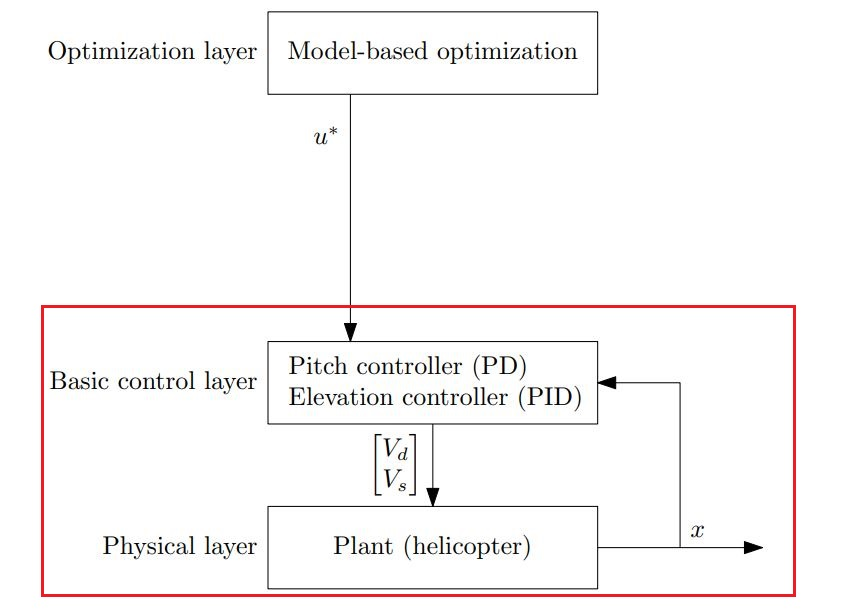
\includegraphics[width=0.8\linewidth]{figures/lab2_system}
	\caption{The red box encapsulate what is modelled in the state space model described by \cref{eq:lab2_cont_ss}.}
	\label{fig:lab2_system}
\end{figure}

This becomes clear studying the equations in \cref{eq:lab2_states_eq}. They describe the helicopters physics for all states except elevation and elevation rate. $ \lambda $ and $ r $ is dependent on the helicopters pitch, $ p $. $ p $ and $ \dot p  $ is however dependent on the voltage difference, $ V_d $. The voltage difference is the output of the PD-controller for controlling the pitch\todo{Should we add acronym list?}. 

To summarize, this means that our state space model describes the helicopter's physics through the dynamic equations for $ \lambda $, $ r $, $ p $ and $ \dot p $, while the equation of $ V_d $ describes the PD-controller used to control the pitch angle. In total our state-space model is modelling both the helicopter and the PD controller for pitch.


\subsubsection{Stability and eigenvalues}
The properties of this system is dependent on physical constants ($l_a, J_t, ...$) and control parameters ($K_{pp}, K_{pd}$).

Symbolic expressions in Matlab shows that the eigenvalues of A are:
\begin{equation}
	\lambda = \pm \frac{1}{2} \left( \sqrt{-K_1 (-K_1 K_{pd}^2 + 4  K_{pp})} - K_1  K_{pd} \right)
\end{equation}

The eigenvalues of the continous model, with $K_{pp} = 0,1 , K_{pd} = 0,4$ are:
\begin{equation}\label{eq:lab2_ss_c_eigenvalues_example}
	\begin{bmatrix}
		0 \\ 0 \\ -0.26 + 0.24i \\ -0.26 - 0.24 \\
	\end{bmatrix}
\end{equation}

% ------------------- DISCRETIZING THE MODEL ------------------------
\subsection{Discretizing the continous time model} \label{sec:lab2_disc}
A discretized model is required for generating an optimal trajectory. \textit{[...] continous time models require quite different solution methods} \cite{FossHeirung}

We will discretize the model using the forward Euler method, which is given by:
\todo[inline]{Do we need to derive forward euler?}
\begin{equation}\label{eq:lab2_forward_euler}
	\bm{x}[k + 1] = \bm I \bm x[k] + T\bm{A_c x}[k] + T\bm B_c ,
\end{equation}
where $ T $ is the sample-time in the discrete model.\todo
[inline]{Add reference to linsys slides}
Reformulating this, we can write:
\begin{equation}\label{eq:lab2_discrete_system}
	\bm{x}_{k + 1} = \underbrace{(\bm I + T \bm A_c)}_{\bm A_d} \bm{x}_{k} + \underbrace{T \bm B_c}_{\bm B_d} u_k
\end{equation}
On matrix form $ \bm A_d $ and $ \bm B_d $ becomes: 
\begin{equation}
	\bm A_d = \begin{bmatrix}
		1 & T & 0 & 0 \\
		0 & 1 & -T K_2 & 0 \\
		0 & 0 & 1 & T \\
		0 & 0 & -T K_1 K_{pp} &  1 - T K_1 K_{pd}
	\end{bmatrix}, \quad 
	\bm B_d = \begin{bmatrix}
		0 \\ 0 \\ 0 \\T K_1 K_{pp}
	\end{bmatrix}
\end{equation}




\subsubsection{Checking stability}
The stability condition for \cref{eq:lab2_discrete_system} is that all eigenvalues of $ \bm A_d $ is less than one in absolute values, i.e.:
\begin{equation}\label{eq:lab2_stab_condition}
	|\lambda_i| \leq 1, \quad \text{for } i = 1, 2, 3, 4
\end{equation}, where $ \lambda_i $ is the i'th eigenvalue of $ \bm A_d $.

Using the script in \cref{lst:lab2_eigenvalues} the eigenvalues became:
\begin{subequations}\label{eq:lab2_eigenvalues}
	\begin{align}
		\lambda_1 &= 1 \\
		\lambda_2 &= 1 \\
		\lambda_3 &= 0.55 \\
		\lambda_4 &= 0.55
	\end{align}
\end{subequations}
All eigenvalues fulfills the requirement of \cref{eq:lab2_stab_condition}, which means our system is stable! Since two of the eigenvalues are on the unit circle (i.e. has a value of 1), our system is more specifically marginally stable. More information on this subject can be found \todo{Add cite to wikipedia}.

\lstinputlisting[caption= {MATLAB code for calculating eigenvalues for $ \bm A_d $}, label = {lst:lab2_eigenvalues}, language=Matlab]{code/calculate_eigenvals.m}

\subsection{The open loop optimization problem}
% https://ntnu.blackboard.com/ultra/courses/_24653_1/cl/outline
%where $q$ is the weight of input-usage. Subject to constraints.
The open loop optimization problem is a constrained quadratic program that can be solved using the Matlab function quadprog. The quadprog function requires the input to be in standard form:

\begin{equation}\label{eq:lab2_quadprog_std_form}
	\min_x \frac{1}{2} \bm x^t \bm H \bm x + \bm f^T \bm x \quad \text{such that} \begin{cases}
		\bm A \bm x \leq \bm b, \\
		\bm A_{eq} \bm x = \bm B_{eq}, \\
		\bm{lb} \leq \bm x \leq \bm{ub}		
	\end{cases}
\end{equation}

The next subsections describes this process.

\subsubsection{Formulating the cost function} \label{sec:lab2_cost_func}
As the problem description states, the cost function used in this exercise is:
\begin{equation} \label{eq:lab2_start_cost_func}
	\phi = \sum_{i=0}^{N-1} \left( \lambda_{i+1} - \lambda_f \right)^2 + qp_{ci}^2 , \quad q \ge 0
\end{equation}

Which can be rewritten with $ \bm x $ and $ u $:
\begin{equation}\label{eq:lab2_start_cost_func_2}
	f(\bm x, u) = \sum_{i=0}^{N-1} \left( \bm x_{i+1} - \bm x_f \right)^T \bm Q \left( \bm x_{i+1} - \bm x_f \right) + q u^2
\end{equation}
where
\begin{equation}\label{eq:lab2_lambda_f}
	\bm x_f = \begin{bmatrix}
		\lambda_f \\ 0 \\ 0 \\ 0
	\end{bmatrix}
\end{equation}
\begin{equation}\label{eq:lab2_Q}
	\bm Q = \begin{bmatrix}
		1 & 0 & 0 & 0 \\
		0 & 0 & 0 & 0 \\
		0 & 0 & 0 & 0 \\
		0 & 0 & 0 & 0
	\end{bmatrix}
\end{equation}
In this case we have that $ \lambda_f = 0 $ and therefore $ \bm x_f = \bm 0 $, and \cref{eq:lab2_start_cost_func_2} can be rewritten as:

\begin{equation}\label{eq:lab2_LQR}
	f(\bm x, u) = \sum_{i=0}^{N-1} \bm x_{i+1}^T \bm Q \bm x_{i+1} + r u^2
\end{equation}
where
\begin{equation}\label{eq:lab2_R}
	r = q
\end{equation}

Defining the the $z$ vector as:
\begin{equation}\label{eq:lab2_z}
	\bm z = \begin{bmatrix}
		\bm x_1 & \bm x_2 & ... & \bm x_n & u_0 & u_1 &... & u_{n-1} 
	\end{bmatrix}^T
\end{equation}
we can rewrite summation form in \cref{eq:lab2_LQR} to matrix-form:
\begin{equation}\label{eq:lab2_quadprog}
	f(\bm z) = \bm z^T \bm H \bm z
\end{equation}
with
\begin{equation}\label{eq:lab2_H}
	\bm H = \begin{bmatrix}
		\bm Q & 0 & \cdots  & 0 & 0 & 0 & \cdots & 0\\
		0 & \bm Q & \cdots  & 0 & 0 & 0 & \cdots & 0\\
		 & & \ddots &  &  &  &  & \\
		0 & 0 & \cdots & \bm Q & 0 & 0  & \cdots & 0\\
		0 & 0 & \cdots & 0 & r & 0  & \cdots & 0\\
		0 & 0 & \cdots & 0 & 0 & r  & \cdots & 0\\
		 & &  &  &  &  & \ddots & \\
		0 & 0 & \cdots & 0 & 0 & 0  & \cdots & r
	\end{bmatrix}
\end{equation}


\subsubsection{The constraints of the optimization problem} \label{sec:lab2_constraints}
There are two separate types of constrains in this problem, the system itself and imposed constraints. The system constrains is described by the physics of the helicopter, which we have modeled in \cref{eq:lab2_discrete_system}. Imposed constraints are constraints added by the designer of the system. 

In this case we have an imposed constraint on the pitch given by:
\begin{equation}
	\left\lvert p_k \right\rvert \le \frac{30}{180} \pi, k \in \left\{ 1, ..., N \right\} 
\end{equation}
As the manipulated variable $ p_c $ is the setpoint for the $ p $ controller, this constraint must also be implemented for the setpoint. Since there is no inequality constraints on the other states, they have lower bounds of $ -\infty $ and upper bounds of $ \infty $. This gives us the inequality constraints for the state and the input as: 
\begin{subequations}
	\begin{align}
		\bm x^{low} = \begin{bmatrix}-\infty \\ -\infty \\ -\frac{30}{180} \pi \\ -\infty \end{bmatrix} &\leq \bm x \leq \bm x^{high} = \begin{bmatrix} \infty \\ \infty \\ \frac{30}{180} \pi \\ \infty \end{bmatrix} \\
		u^{low} = -\frac{30}{180} \pi &\leq u \leq u^{high} = -\frac{30}{180} \pi
	\end{align}
\end{subequations}
We can now easily expand this to define lower- and upper-bounds for the vector $ \bm z $ given in \cref{eq:lab2_z}
\begin{equation}\label{eq:lab2_z_bounds}
		\bm z^{low} = \begin{bmatrix}
			\bm x^{low}\\
			\vdots \\
			\bm x^{low}\\
			u^{low}\\
			\vdots \\
			u^{low}
		\end{bmatrix} \leq \bm z \leq
		\bm z^{high} = \begin{bmatrix}
			\bm x^{high}\\
			\vdots\\
			\bm x^{high}\\
			u^{high}\\
			\vdots \\
			u^{high}\\
		\end{bmatrix}
\end{equation}



The system constraints can be defined as: 
\begin{equation}\label{eq:lab2_physical_constraints}
	\bm A_{eq} \bm z = \bm b_{eq}
\end{equation}
, where
%The physics of the helicopter is added in $A_{eq}$ and $b_{eq}$.
\begin{equation} \label{eq:lab2_Aeq_beq}
	\bm A_{eq} = 
	\begin{bmatrix}
		\bm I & 0 & \cdots & \cdots & 0 & -\bm B_d & 0 & \cdots & \cdots & 0 \\
		-\bm A_d & \bm I & \ddots & & \vdots & 0 & \ddots & \ddots & & \vdots \\
		\vdots && \ddots & \ddots & 0 & \vdots & & \ddots & \ddots & 0 \\
		0 & \cdots & 0 & -\bm A_d & \bm I & 0 & \cdots & \cdots & 0 & -\bm B_d
	\end{bmatrix}, \; 
	\bm b_{eq} =
	\begin{bmatrix}
		\bm A_d \bm x_0 \\ 0 \\ \vdots \\ 0
	\end{bmatrix}
\end{equation}

Performing the multiplication (and abusing notation) shows that:
\begin{equation} \label{eq:lab2_system_constraints}
	\bm A_{eq} \bm z = \bm b_{eq} \implies
	\begin{bmatrix}
		\bm x_1-\bm B_d u_0 = \bm A_d \bm x_0 \\
		-\bm A_d \bm x_1 + \bm x_2 - \bm B_d u_1 = 0 \\
		\vdots \\
		-\bm A_d \bm x_{n-1} + \bm x_n - \bm B_d u_{n-1} = 0 \\
	\end{bmatrix} \implies
	\begin{bmatrix}
		\bm x_1 = \bm A_d \bm x_0 + \bm B_d u_0 \\
		\bm x_2 = \bm A_d \bm x_1 + \bm B_d u_1 \\
	 	\vdots \\
		\bm x_n = \bm A_d \bm x_{n-1} + \bm B_d u_{n-1}
	\end{bmatrix}
\end{equation}
\Cref{eq:lab2_system_constraints} describes the system in terms of \cref{eq:lab2_discrete_system} for all timesteps\todo{Again: timesteps illegal?}, and thereby also describes all system constraints for the system.

\subsubsection{Defining the open loop optimization problem}
Combining the cost function described in \cref{sec:lab2_cost_func} and the constraints described in \cref{sec:lab2_constraints} the open loop optimization problem can be defined as: 

\begin{equation}\label{eq:lab2_open_loop_opt_problem}
	f(\bm z) = \bm z^T \bm  H \bm z \quad \text{s.t.} \quad 
	\begin{cases}
		\bm A_{eq} \bm z = \bm B_{eq} \\
		\bm z^{low} \leq \bm z \leq \bm z^{high}
	\end{cases} 
\end{equation}, 
where $ \bm z $ is given by \cref{eq:lab2_z}, $ \bm H $ is given by \cref{eq:lab2_H}, $ \bm A_{eq} $ and $ \bm B_{eq} $ is given by \cref{eq:lab2_Aeq_beq}, and $ \bm z_{low} $ and $ \bm z_{high} $ is given by \cref{eq:lab2_z_bounds}.

It is now easy to compare this to the QP formulation given in \cref{eq:lab2_quadprog_std_form}, and implement this in MATLAB. This is done in \cref{lst:lab2_matlab}. 

\textbf{NB:} that the variable names are not exactly the same in the code as in the sections above, but the procedure is the same.

\subsection{The weights of the optimization problem}
\textit{Try using the values 0.1, 1 and 10 as weights q. Plot the manipulated variable and the output. Comment the results with respect to the different weights chosen.}

$ \bm Q $ and $ r $ in \cref{eq:lab2_LQR} are typically called weight-matrices. Their relative values reflect how the LQ regulator prioritize the objectives (the state and the input) relative ot each other. In this problem, $ \bm Q $ is kept constant and the group changed the value of $ r $ (or $ q $ as it is called in the problem description). Increasing the value of $ q $ means that we are placing a higher cost of input - reducing the input usage. In other words, a smaller $ q $ will make the ``fuel'' (or input) expensive. 
%This will in turn mean that the cost of deviation in $\lambda$ is, in relation to the input, cheaper. 
The result is lower input usage and a slower response. This is exactly what is seen in \cref{fig:lab2_optimalu}.

\begin{figure}[h]
	\centering
	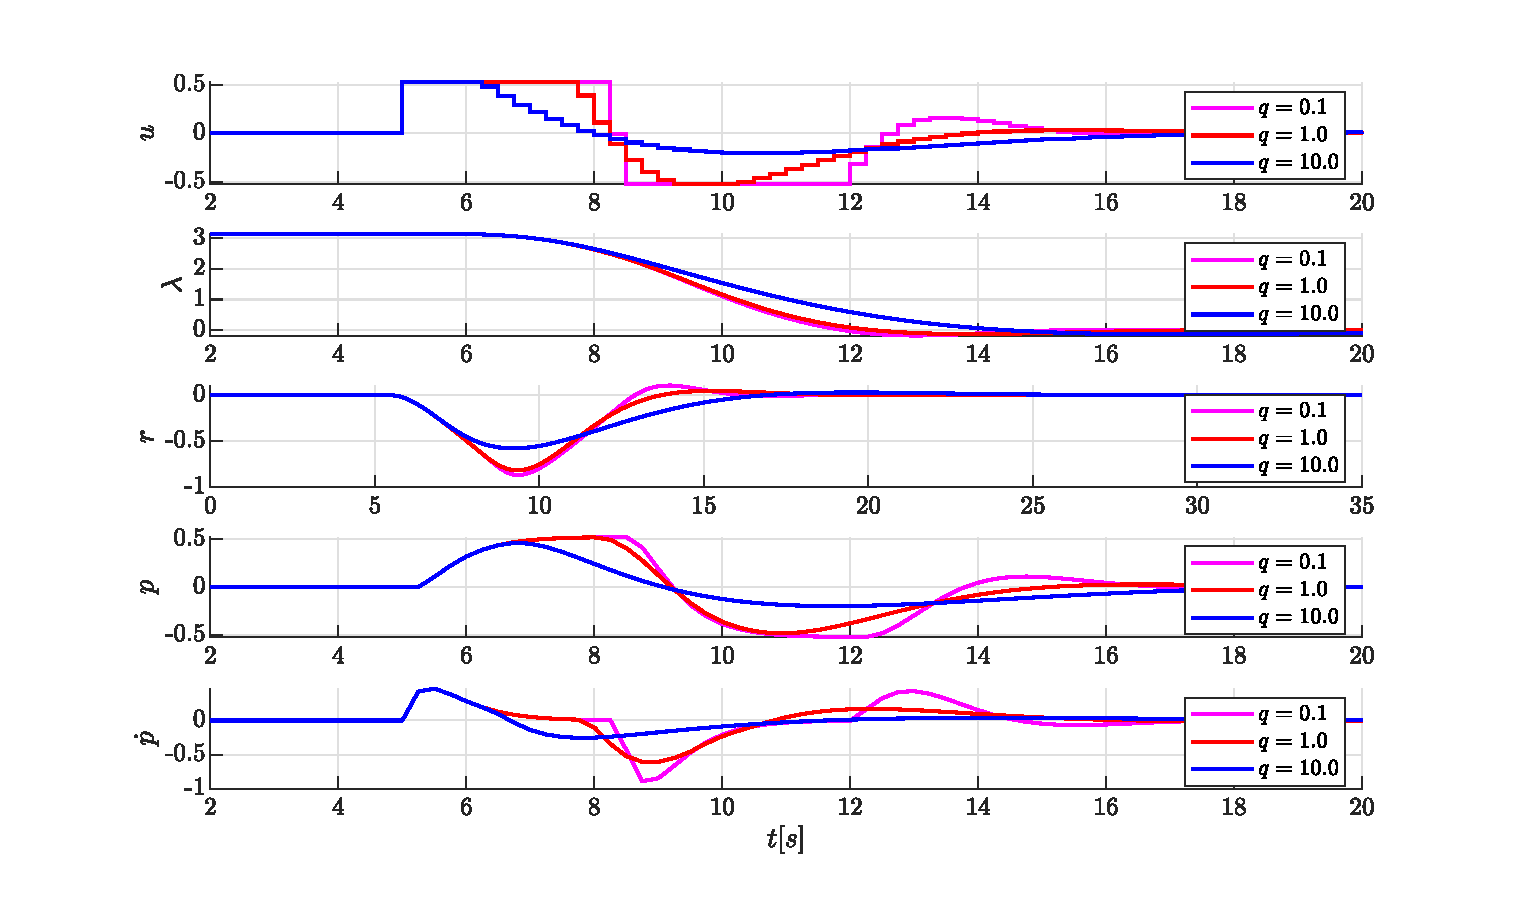
\includegraphics[width=\linewidth]{figures/lab2_optimal_u}
	\caption{Optimal trajectories for the manipulated variable and outputs with different values of $q$.}
	\label{fig:lab2_optimalu}
\end{figure}

\Cref{fig:lab2_optimalu} also shows how the constraints work in practice. Studying the plot of $ u $, we can see that no matter how low $ q $ is, the input never goes beyond the specified range of $ \pm\frac{30}{180} \pi $.

\subsection{The objective function}
\textit{Furthermore, discuss the objective function (15) (in the lab assignment text) in particular the term $(\lambda_i-\lambda_f )^2$. For instance, could any unwanted effects arise from steering the helicopter to $\lambda =\lambda_f$ with this objective function?}

The term $(\lambda_i-\lambda_f )^2$ in \cref{eq:lab2_start_cost_func} may cause problems if it becomes too large compared to the term $ q \cdot u^2 $. What is meant by ``too large'' is that the solution will actually never reach $ \lambda_f $ in the given time horizon, because it is theoretically impossible due to the problem constraints. \Cref{fig:lab2_too_large} shows this. This is the solution of the optimization problem when the group used $ \lambda_0 = 40\pi $. It shows that when the error term for the travel is too large, the helicopter will never reach $ \lambda_f $ no matter what. A direct consequence of this is that the helicopter will never stop the rotation before the time horizon ends.
\begin{figure}[h]
	\centering
	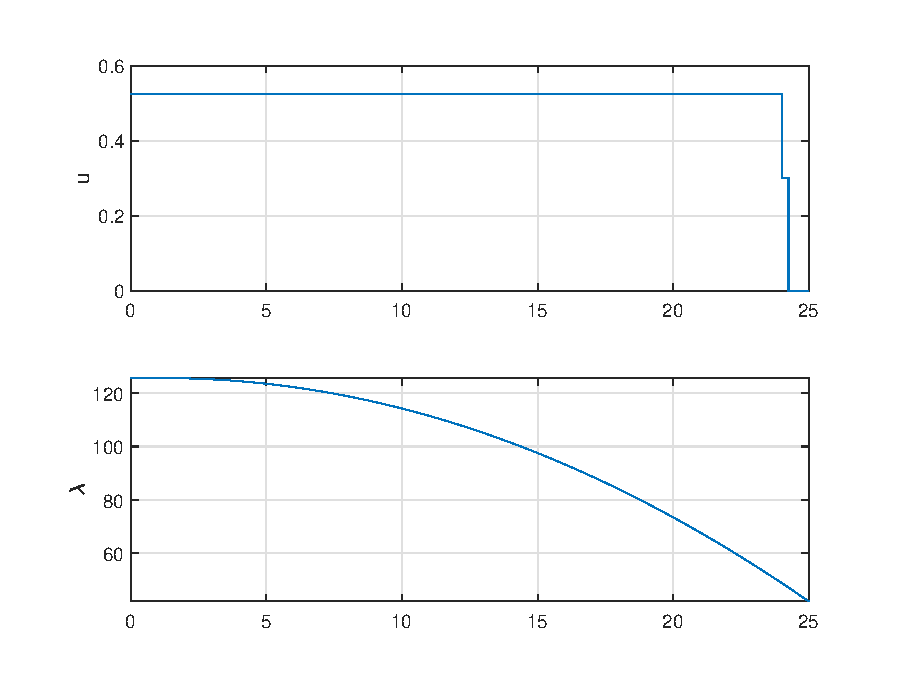
\includegraphics[width=\linewidth]{figures/lab2_1_5_example.eps}
	\caption{Optimal trajectories using $\lambda_0 = 40\pi$ .}
	\label{fig:lab2_too_large}
\end{figure}
\Cref{fig:lab2_too_large} also shows that increasing $(\lambda_i-\lambda_f )^2$ has the same effect as increasing $ \bm Q $ relative to $ r $ in \cref{eq:lab2_LQR}; it will prioritize to minimize $(\lambda_i-\lambda_f )^2$ and use much input to achieve this. We say that the ``fuel'' is cheap.

The ``solution'' to this problem is to increase the time horizon either by adding more steps (increase $N$) or increase the sampling time. This will give the optimization problem enough time to reach the $ \lambda_f $. This is shown in \cref{fig:lab2_inc_delta_t}. In this case the sampling time was doubled from $ 0.25 $ to $ 0.5 $, and the optimization problem had almost enough time to stop rotating at the final value. 
\begin{figure}[h]
	\centering
	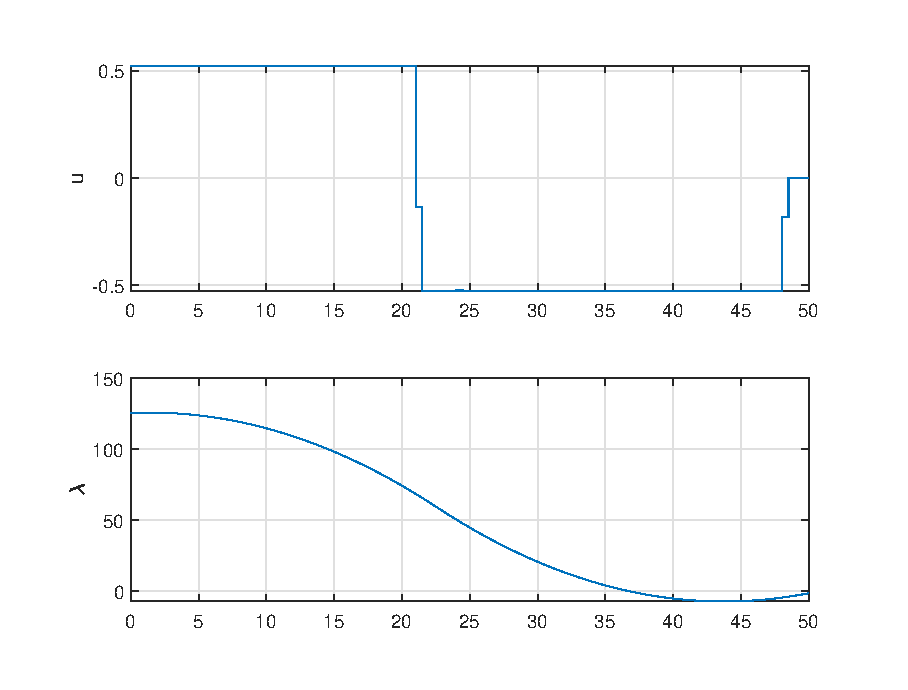
\includegraphics[width=\linewidth]{figures/lab2_1_5_example_2.eps}
	\caption{Optimal trajectories using $\lambda_0 = 40\pi$ and $ \Delta t = 0.5$ .}
	\label{fig:lab2_inc_delta_t}
\end{figure}

\subsubsection{Improved $ \lambda_0 $ selection}
In the case of the lab setup, it does not really make any sense to have $ \lambda_i-\lambda_f >  2\pi $, because the helicopter is always on a circles edge. The result of this is that $ \lambda = 0 $, $ \lambda = 2\pi $ and $ \lambda = 4\pi $ and so on, is essentially the same helicopter-configuration. 

Also, the way the objective function is set up, it will not choose the always choose the shortest way to $ \lambda_f $. If $ \lambda_0 = \frac{3}{4} \pi $, this means that the helicopter is $\frac{3}{4} \pi $ radians from $ \lambda_f $ in the counter-clockwise direction and  $\frac{1}{4} \pi $ radians from  $ \lambda_f $ in the clockwise direction. Therefore, it is most logical to go the clockwise direction, because this requires the least amount of input. However, the way the objective function is chosen, it will go in the counter-clockwise direction.

Therefore, a suggested solution from the group, is to use the following formula for $ \lambda_0 $: 
\begin{subequations}
	\begin{align}
		\lambda_{0, \text{modified}} &= \begin{cases}
			+\text{mod}(\lambda_0-\lambda_f, 2\pi), \quad &\text{if} \quad \text{mod}(\lambda_0-\lambda_f, 2\pi) \leq \pi \\
			-(2 \pi - \text{mod}(\lambda_0-\lambda_f, 2\pi)) \quad &\text{else}
		\end{cases} \\ 
	\end{align}
\end{subequations}, where $ \text{mod} $ is the modulus operator.

This will insure that $ \lambda_i-\lambda_f \leq  2\pi $ for all $ i \in (0, 1, 2, ..., N-1) $ and it will also insure that the helicopter will choose the shortest direction.

It is easily implemented in the code, as \cref{lst:improved_lambda_0} shows.
\begin{lstlisting} [caption={Improved $\lambda_0$ implementation.}, label={lst:improved_lambda_0}]
	lambda_0 = 4/3*pi; %Some value
	lambda_0 = mod(lambda_0, 2*pi);
	if (lambda_0 > pi)
		lambda_0 = -(2*pi - lambda_0);
	end
\end{lstlisting} 

\clearpage
\subsection{Experimental results}\label{kap:task_10_2_experimental_results}
The group performed two experiments with the helicopter:
\begin{enumerate}
	\item Flight with optimal setpoints: $u_k = u_k^*$
	\item Flight without setpoints: $u_k = 0$
\end{enumerate}
Both fligths, along with the optimal trajectory and a compensated trajectory are plotted in \cref{fig:LAB2_plot_1}.

\begin{figure}[h]
	\centering
	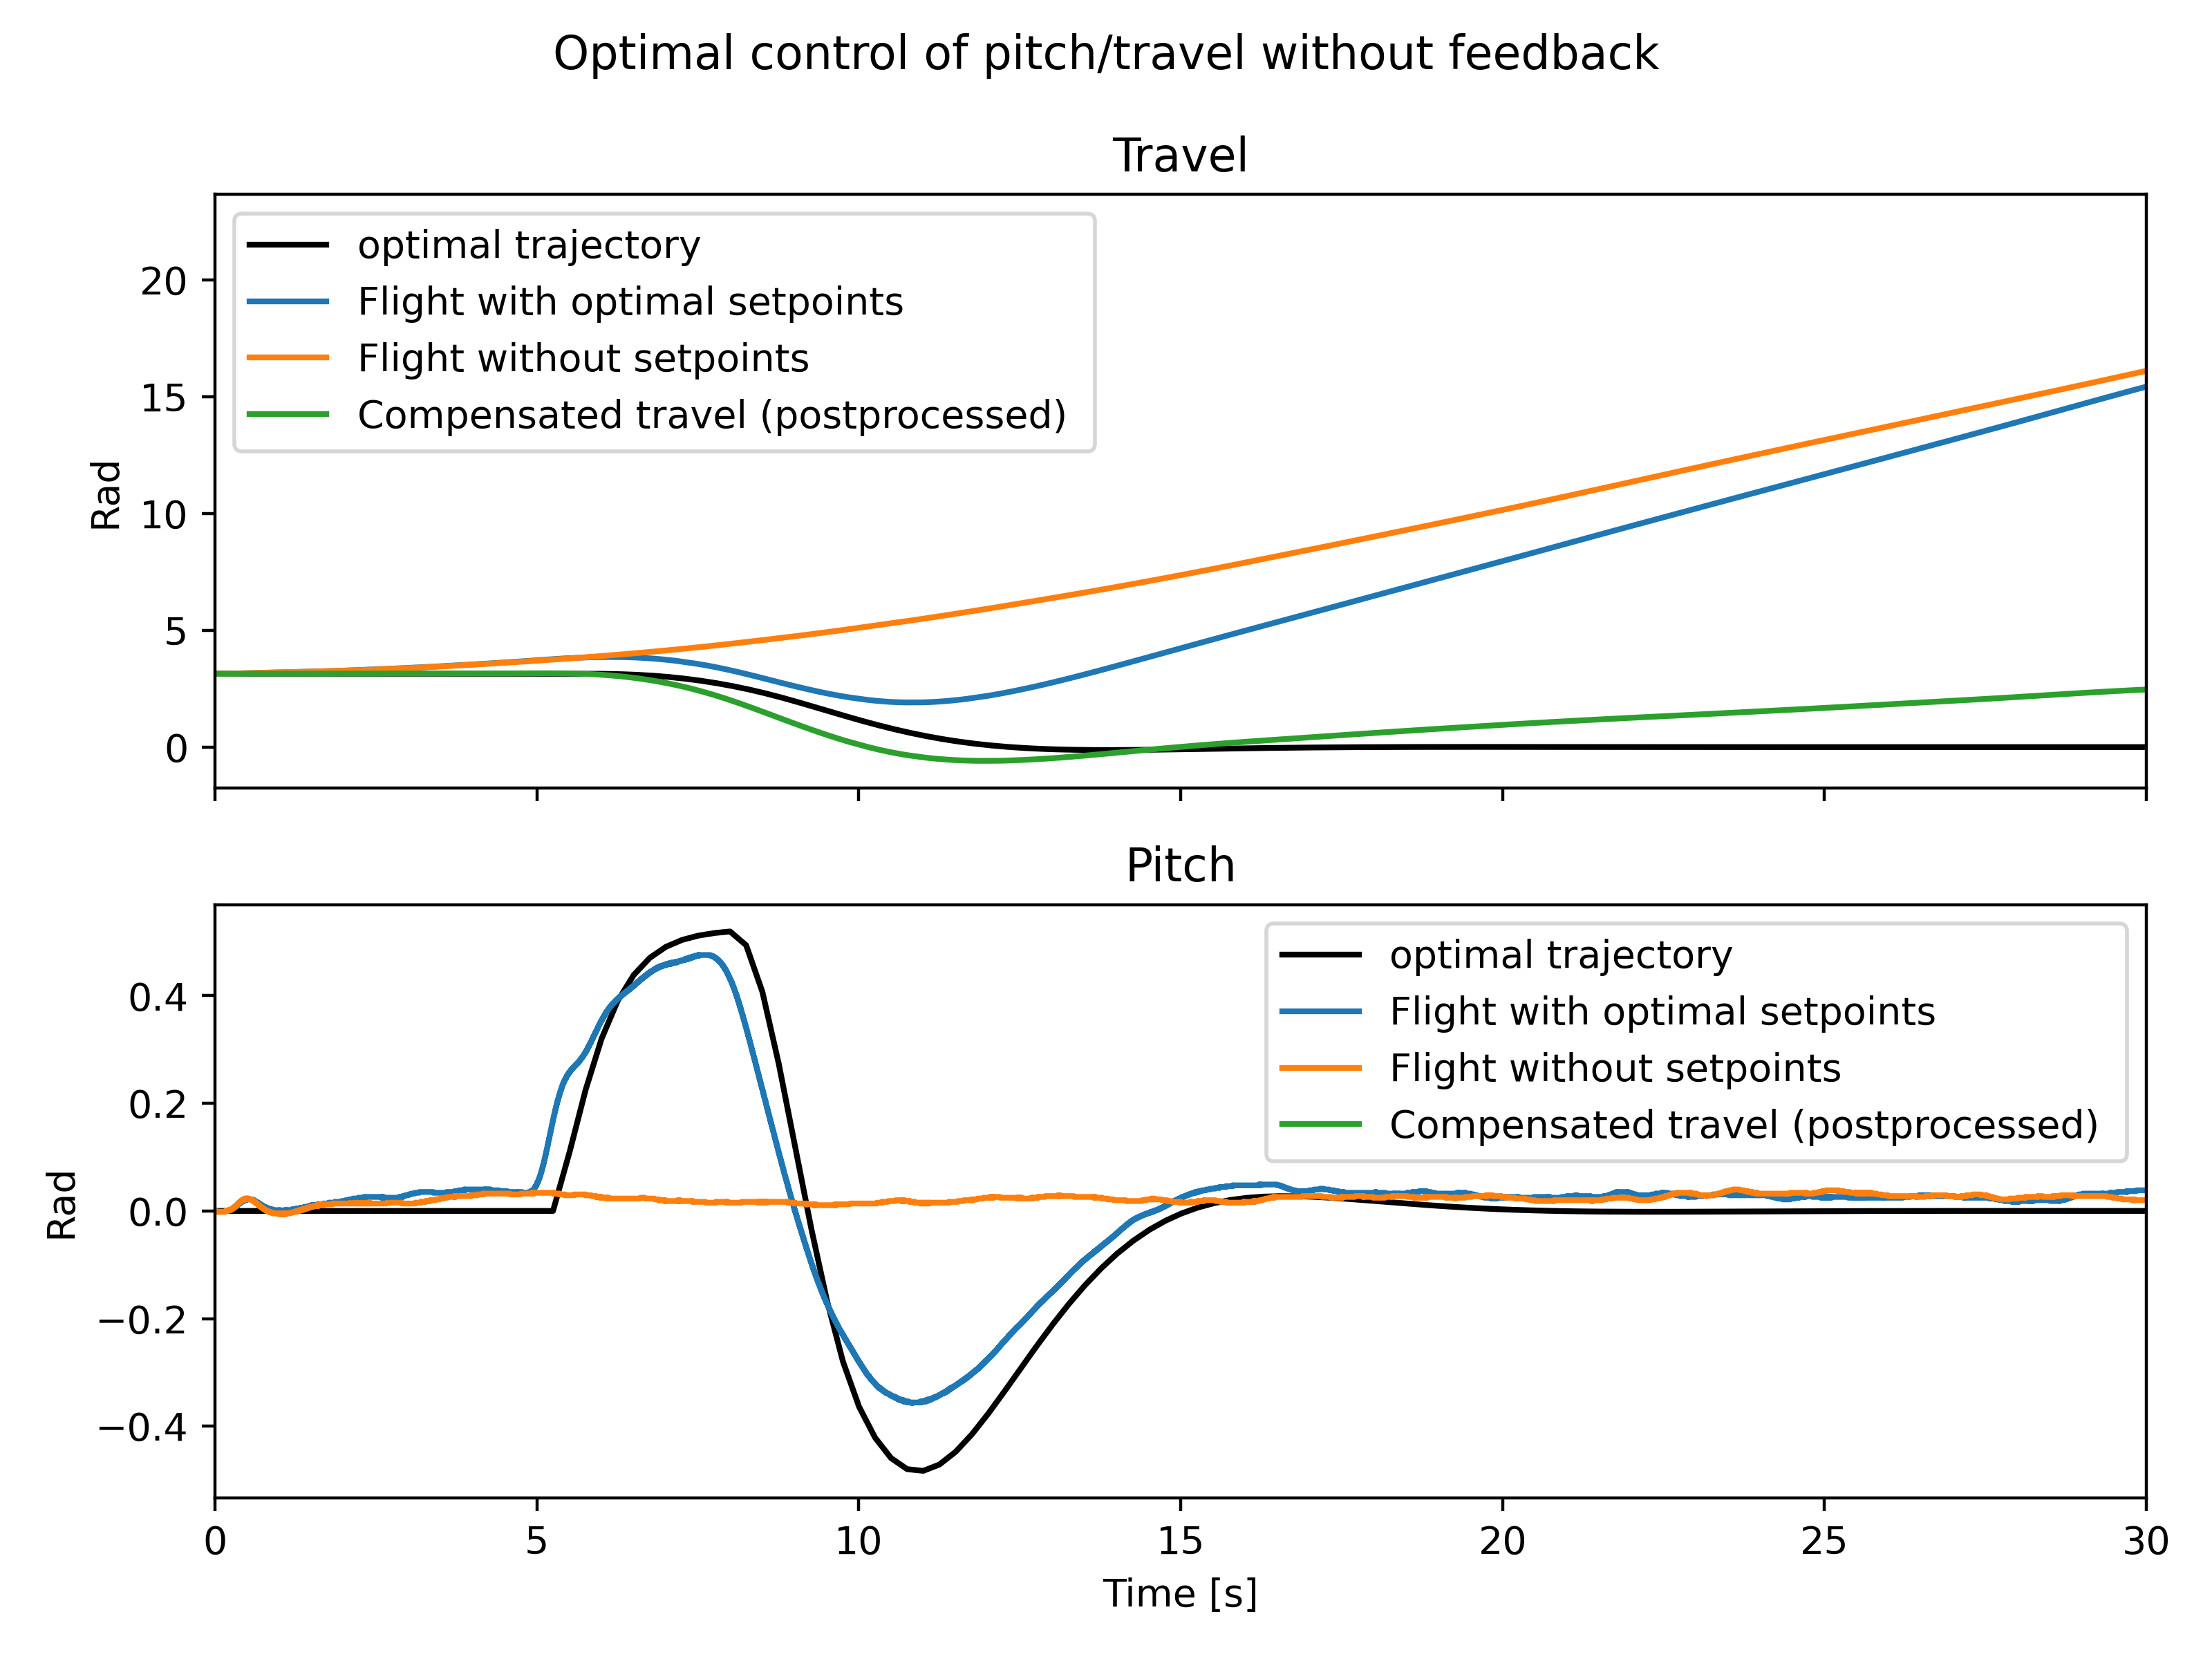
\includegraphics[width=0.8\linewidth]{figures/LAB2_plot_1.png}
	\caption{Results of LAB2}
	\label{fig:LAB2_plot_1}
\end{figure}

\subsubsection{Pitch-control}
It is clear that both fligths have adequate control of pitch. In the case where $u_k = 0$ the pitch is close to $0$. In the case where $u_k = u_k^*$ the pitch is close to the optimal trajectory.

This is expected as pitch-control is a closed loop - the basic control layer has a PD controller that ensures that pitch follows the reference $u_k$.

\subsubsection{Travel-drift}\label{kap:LAB2_travel_drift_causes}
From the flight with $u_k = 0$ it is clear that there is significant travel-drift present in the helicopter. Even when pitch is very close to $0$ the helicopter travels quickly far away from the initial point.

There are three main causes of drift:
\begin{enumerate}
	\item The encoder-measurement of pitch is not precise
	\item Helicopter inbalance
	\item Disturbances
\end{enumerate}

When the helicopter starts, it reads the initial \textbf{encoder}-value for the pitch, and assumes this is equal to zero. However, if the platform is not built precisely, the encoder axis may not be 100 \% aligned with the corresponding real world axis. There are many possible reasons for this, but it will not be discussed further. Regardless of the cause, the effect will be the same: The measured encoder-value will have a constant offset compared to real world-values. This will again cause the helicopter to drift when it measures zero pitch.

%The \textbf{encoder} does not measure pitch at the helicopter in relation to gravity, rather it measures the angle between the helicopter blades and the platform that holds them. Because that platform is not build to be precisely the same as gravity (and because of wear-and-tear) the measured value $0$ is not exactly 0. This causes the helicopter to have a pitch offset, which in turn generates travelrate and travel.

The \textbf{imbalance} may be that one rotor is stronger than the other, or that the rotors have offsets from the vertical position. These imbalances may generate a sidewards force, even when the helicopter is pitched to $0$, which in turn generates travelrate and travel.

The \textbf{disturbances} is the most general effect. Air-pressure, wind, temperature effects, walls, and so on. All of these disturbances may cause drifts or noise in the travel. 

The group believes that the main cause of the drift observed in the helicopter is the offset in the encoder.

\subsubsection{Conclusion}
As \cref{fig:LAB2_plot_1} clearly shows the control sequence did not yield the desired travel-response. This was expected, as there are many causes of drift and disturbances. Without any feedback the helicopter will quickly deviate from the desired response, since it will not have any mechanisms to detect deviations from the optimal trajectories.

Nevertheless it is possible to verify the control sequence by compensating for the drift. The compensation can be done by taking the travel of the flight with optimal setpoints, and subtracting the drift logged in the flight without setpoints (i.e. $ u_k = 0 $). The result is plotted as compensated travel in \cref{fig:LAB2_plot_1}. This clearly shows that without the major drift the helicopter would be much closer to the optimal trajectory.


\clearpage
\subsection{MATLAB and Simulink}
\subsubsection{MATLAB}
\lstinputlisting[caption= {MATALB code for lab 2}, label={lst:lab2_matlab}]{code/lab2.m}
\clearpage
\subsubsection{Simulink}
\begin{figure}[h]
	\centering
	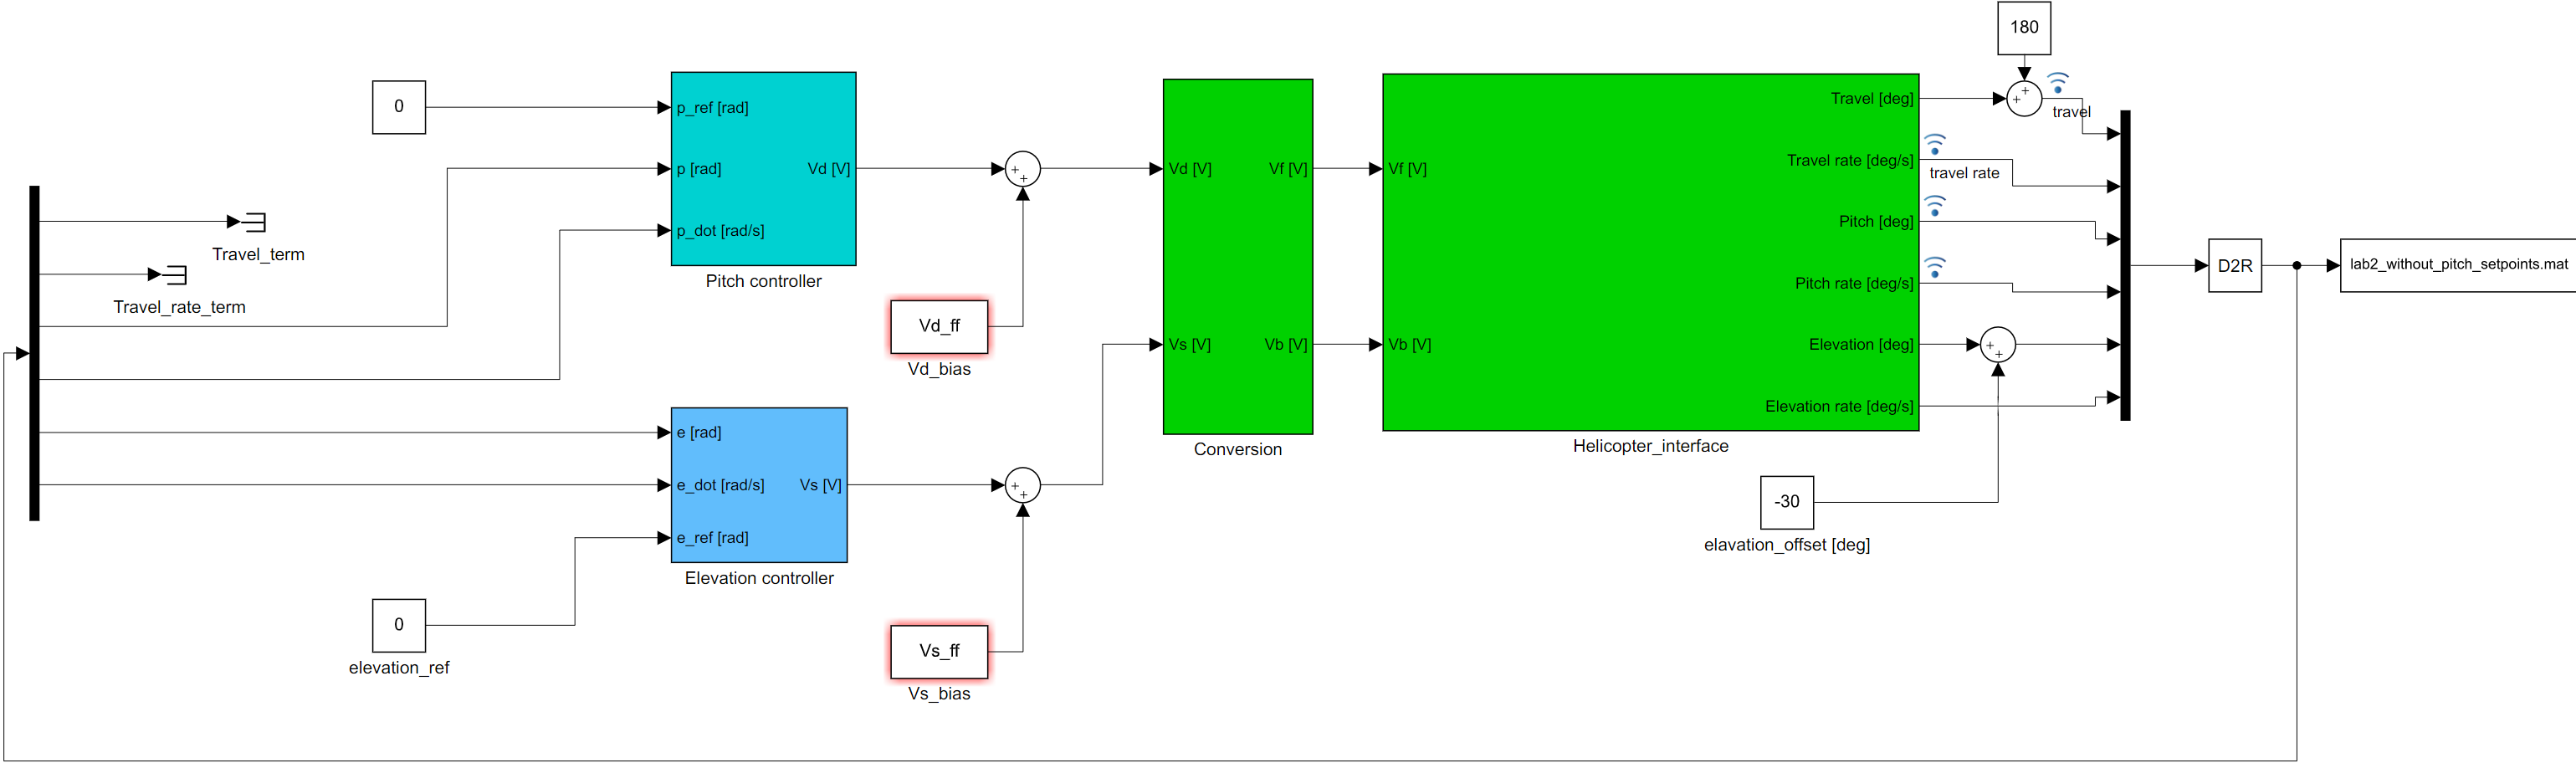
\includegraphics[angle=90, width=0.5\textwidth,height=0.7\textheight]{code/lab2_simulink}
	\caption{Simulink diagram used in lab 2.}
	\label{fig:lab2_simulink}
\end{figure}
\end{document}
\documentclass[../main.tex]{subfiles}
\begin{document}

\section{Optimal Control of Pitch/Travel with Feedback (LQ)}  \label{sec:lab3}
In this task we add feedback to the optimal controller that we developed in \cref{kap:Part2OptimalControlWithoutFeedback}.

\subsection{Motivation}
The experimental results in \cref{kap:task_10_2_experimental_results} clearly shows that planning a sequence of inputs does not produce the expected sequence of outputs - as that section explains there are many reasons for travel-drift. In situations with drift without feedback then the output will not follow the planned trajectory, but adding feedback could compensate for the drift and offset and therefore reduce or eliminate the deviation from the planned trajectory.

The results achieved in this section shows that adding feedback greatly improves performance.

\subsection{Introducing feedback}
There are many approaches to adding feedback, but in this assignment only two will be considered: linear state feedback and model predictive control.

\textbf{Linear state feedback} adds a new control layer below the optimization layer, the advanced control layer, that controls the setpoint to the pitch controller. The setpoint is determined from a control law that considers the optimal trajectory and the current state of the system. If the states deviate from the optimal value the input is changed according to the pitch-control equation:
\begin{equation}\label{eq:lab3_feedback}
	u_k = u_k^* - \bm{K}^T(\bm x_k - \bm x_k^*)
\end{equation}
where $u_k^*$ and $\bm x_k^*$ are the optimal input and state trajectories predicted in the optimization layer, $u_k$ is the next input and $x_k$ is the current state. $K$ is the linear state feedback gain. 

In this exercise the gain matrix $K$ is calculated as an infinite horizon LQ controller, see \cref{kap:task_10_3_LQ_controller} for more info about the exact implementation.

\textbf{Model Predictive Control (MPC)} is a completely different solution: the optimal trajectory is recalculated at every timestep - instead of compensating for deviation from optimal, the optimal is recalculated to get a new possible trajectory based on the current states. See \cref{kap:10_3_mpc} for more info about how that could be implemented here.

\subsection{LQ controller} \label{kap:task_10_3_LQ_controller}
A Linear Quadratic (LQ) controller minimizes the quadratic objective function:
\begin{equation}
    J = \sum^\infty_{i=0} \Delta x_{i+1}^\top Q \Delta x_{i+1} + \Delta u_i^\top R \Delta u_i, \quad Q \ge0, \quad R > 0
\end{equation}
for a linear model
\begin{equation}\label{eq:lab3_lin_model}
	\Delta x=A\Delta x_i + B \Delta u_i
\end{equation}
Here $ \Delta x = x - x^*$ and $\Delta u = u - u^*$ are deviations from the optimal trajectory.

This formulation is an infinite horizon linear quadratic regulator which has a solution with a constant linear feedback gain, $K$ - which is exactly what was specified previously! Note that this regulator does not have any constraints.

\subsubsection{Choosing the weights} 
The matrix $Q$ and the scalar $R$ are the weights of the optimalization problem. $Q$ determines how much state-deviations should be penalized, while $R$ determines how much input-deviation should be penalized. What needs to prioritized depends on the application.

In this case the system is a helicopter where the goal is to control the travel of the helicopter. The travel is the most important state, while travelrate, pitch and pitchrate are secondary. Thus it makes sense to prioritize keeping travel close to the planned trajectory - it is of course not possible to keep all states close to the trajectory. This motivates a \textbf{state-weight} with relatively high value related to travel.

The LQR regulator controls the pitch-setpoint that in turn controls travel. In the end controlling travel is the most important - a deviation in setpoint from the predicted optimal is completely fine as this is how travel is regulated. Thus a low input-weight is warranted as that allows the setpoint to deviate further from the planned trajectory.

\subsubsection{Respecting constraints}
The pitch-setpoint in the optimalization layer has a constraint, see \cref{sec:lab2_constraints} - but the implementation of LQR controller does not respect this constraint! The result is that the pitch-setpoint could fall outside the constraint imposed in the optimalization layer. This does in fact happen, for instance in \cref{fig:LAB3_Q_variations_travel}, where the setpoint is outside the constraint ($\approx 0.52 rad $).

The simplest solution to this problem is to respect the constraint by saturating the output of the regulator to that value. However that does makes impossble for the LQ regulator to compensate in cases where the input is already constrained, therefore it would make sense to set the saturation limit slightly higher than the constraint value to allow the regulator to work in such cases (or equivalently set the constraint lower than the saturation point).

\subsubsection{Calculating the solution}
Calculating the solution to the LQR problem is trivial using Matlab:
\begin{lstlisting}[language=Matlab]
% The discrete system described as a state space system, Ad and Bd must be defined

% W1 is the weigth of travel
% W2 is the weight of travelrate
% W3 is the weight of pitch
% W4 is the weight of pitchrate
Q = diag([W1, W2, W3, W4]);

% W5 is the weight of the input
R = W5;

% The function dlqr is used to solve the LQR problem
[K, S, e] = dlqr(Ad, Bd, Q, R);
\end{lstlisting}

\subsection{Model Predictive Control}\label{kap:10_3_mpc}
Model Predictive Control is another way of introducing feedback to an optimal control system. In an MPC controlled system the optimal response and input is recalculated at every timestep, the input used is simply the first of the optimal input values calculated at every step.

This is a drastically different approach to the LQ-method impemented in this laboratory exercise.

\subsubsection{Implementing MPC}
Implementing MPC requires a system model, cost function, current state and input control.

One could make a Matlab function that the simulink model uses at every timestep. The input to this function is the current state (either measured or estimated), while the output is connected to the pitch-regulator. The function itself has a model of the system as well as the cost function - with the state from the system the optimalization problem can be solved and the first system-input is returned to the simulink model. 

\subsubsection{Advantages of MPC}
The biggest advantage of MPC compared to the linear state feedback introduced here, is that MPC generates a new optimal trajectory that is more realistic for the helicopter to achieve. Since the optimal trajectory is recalculated based on the current state, the helicopter's response will achieve smaller errors compared to the optimal trajectory. 

%Imagine a situation where the helicopter needs to fly below some obstacle. A deviation in elevation that would cause a collision with the obstacle might not be corrected before travel reaches the obstacle - MPC would slow down travel enough to have a trajectory that is possible to achieve.

Another advantage is that MPC allows for feedback with explicitly defined constraints. This is a more intuitive way of keeping the helicopter stable and within the wanted working-range, compared to looking at eigenvalues of the system matrix with linear state feedback.

\subsubsection{Disadvantages of MPC}
The biggest disadvantage to MPC is complexity and computation time - in a control system there are hard deadlines and if the optimalization problem has not been solved within that deadline, the system has a problem.

First of all the problem must be simple enough or optimized enough to solve at every timestep. If this is not achievable the problem must be simplified/optimized or the timestep must be increased. The time to solve a problem can also vary, which makes this issue more complex.

Another issue is \textbf{existence of solutions} must be guaranteed for all situations. It is possible to have problems that have solutions in some configurations, while being undefined for others. Our helicopter is far from perfect, and our model is quite simple. These imperfections may cause the helicopter's configuration to go outside the defined constraints. This could cause the helicopter to freeze mid-air because there was no solution. If these border cases was not taken care of during implementation, this could be fatal.

\subsubsection{Modified Control Hierarchy with MPC}

\begin{figure}[h]
	\centering
	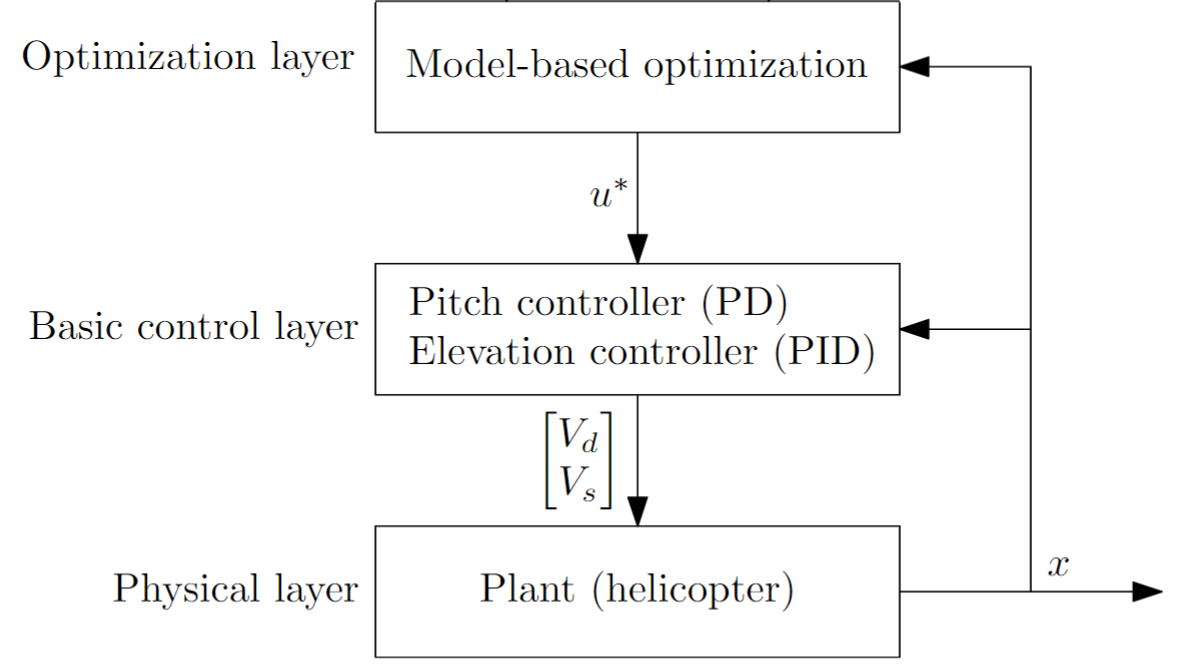
\includegraphics[width=0.7\linewidth]{content/MPC control hierarchy.png}
	\caption{The control hierarchy would look like this using MPC.}
\end{figure}

\subsection{Experimental results}\label{sec:lab3_result}
The group performed a host of controlled tests with different tunings within five different targets:
\begin{enumerate}
	\item Prioritizing input use, see \cref{fig:LAB3_R_variations}
	\item Prioritizing travel, see \cref{fig:LAB3_Q_variations_travel}
	\item Prioritizing travelrate, see \cref{fig:LAB3_Q_variations_travelrate}
	\item Prioritizing pitch, see \cref{fig:LAB3_Q_variations_pitch}
	\item Prioritizing pitchrate, see \cref{fig:LAB3_Q_variations_pitchrate}
\end{enumerate}

It is very clear that introducing feedback produced results much better than the ones achieved without feedback, almost regardless of the tuning of the LQR regulator.

Prioritizing input usage only has a slight effect, the input usage does get slightly closer to the planned trajectory but not by much. This could of course be pushed further by weighing states lower or input higher, but this was not explored - if the input is regulated very close to the planned trajectory then the result is the same as the previous lab-exercise where u was exactly equal to the planned trajectory.

Prioritizing travel has a great effect on the travel response - resulting in almost perfect travel response. Unfortunately this also introduced oscillations in pitch-setpoint, pitch and pitchrate.

Prioritizing travelrate, pitch and pitchrate results in responses closer to the corresponding planned trajectory, but this is not further discussed as travel is the state most important to control - theese experiments were only to show that it would be possble should another state be valuable.

\subsubsection{Possible improvements}
The group observed that the state never reached the optimal trajectory, even with very high Q-values. The group believes that adding integration to the LQ-regulator would eliminate the stationary offset between travel and the planned travel trajectory.

Another possible improvement would be to change the cost function in the optimalization layer to generate a trajectory that is easier for the helicopter to follow. There is not guarantee that it is physically possible for the helicopter to follow the trajectory generated here, because the model of the system is not perfect.

\subsubsection{Plots}

\begin{figure}[h]
	\centering
    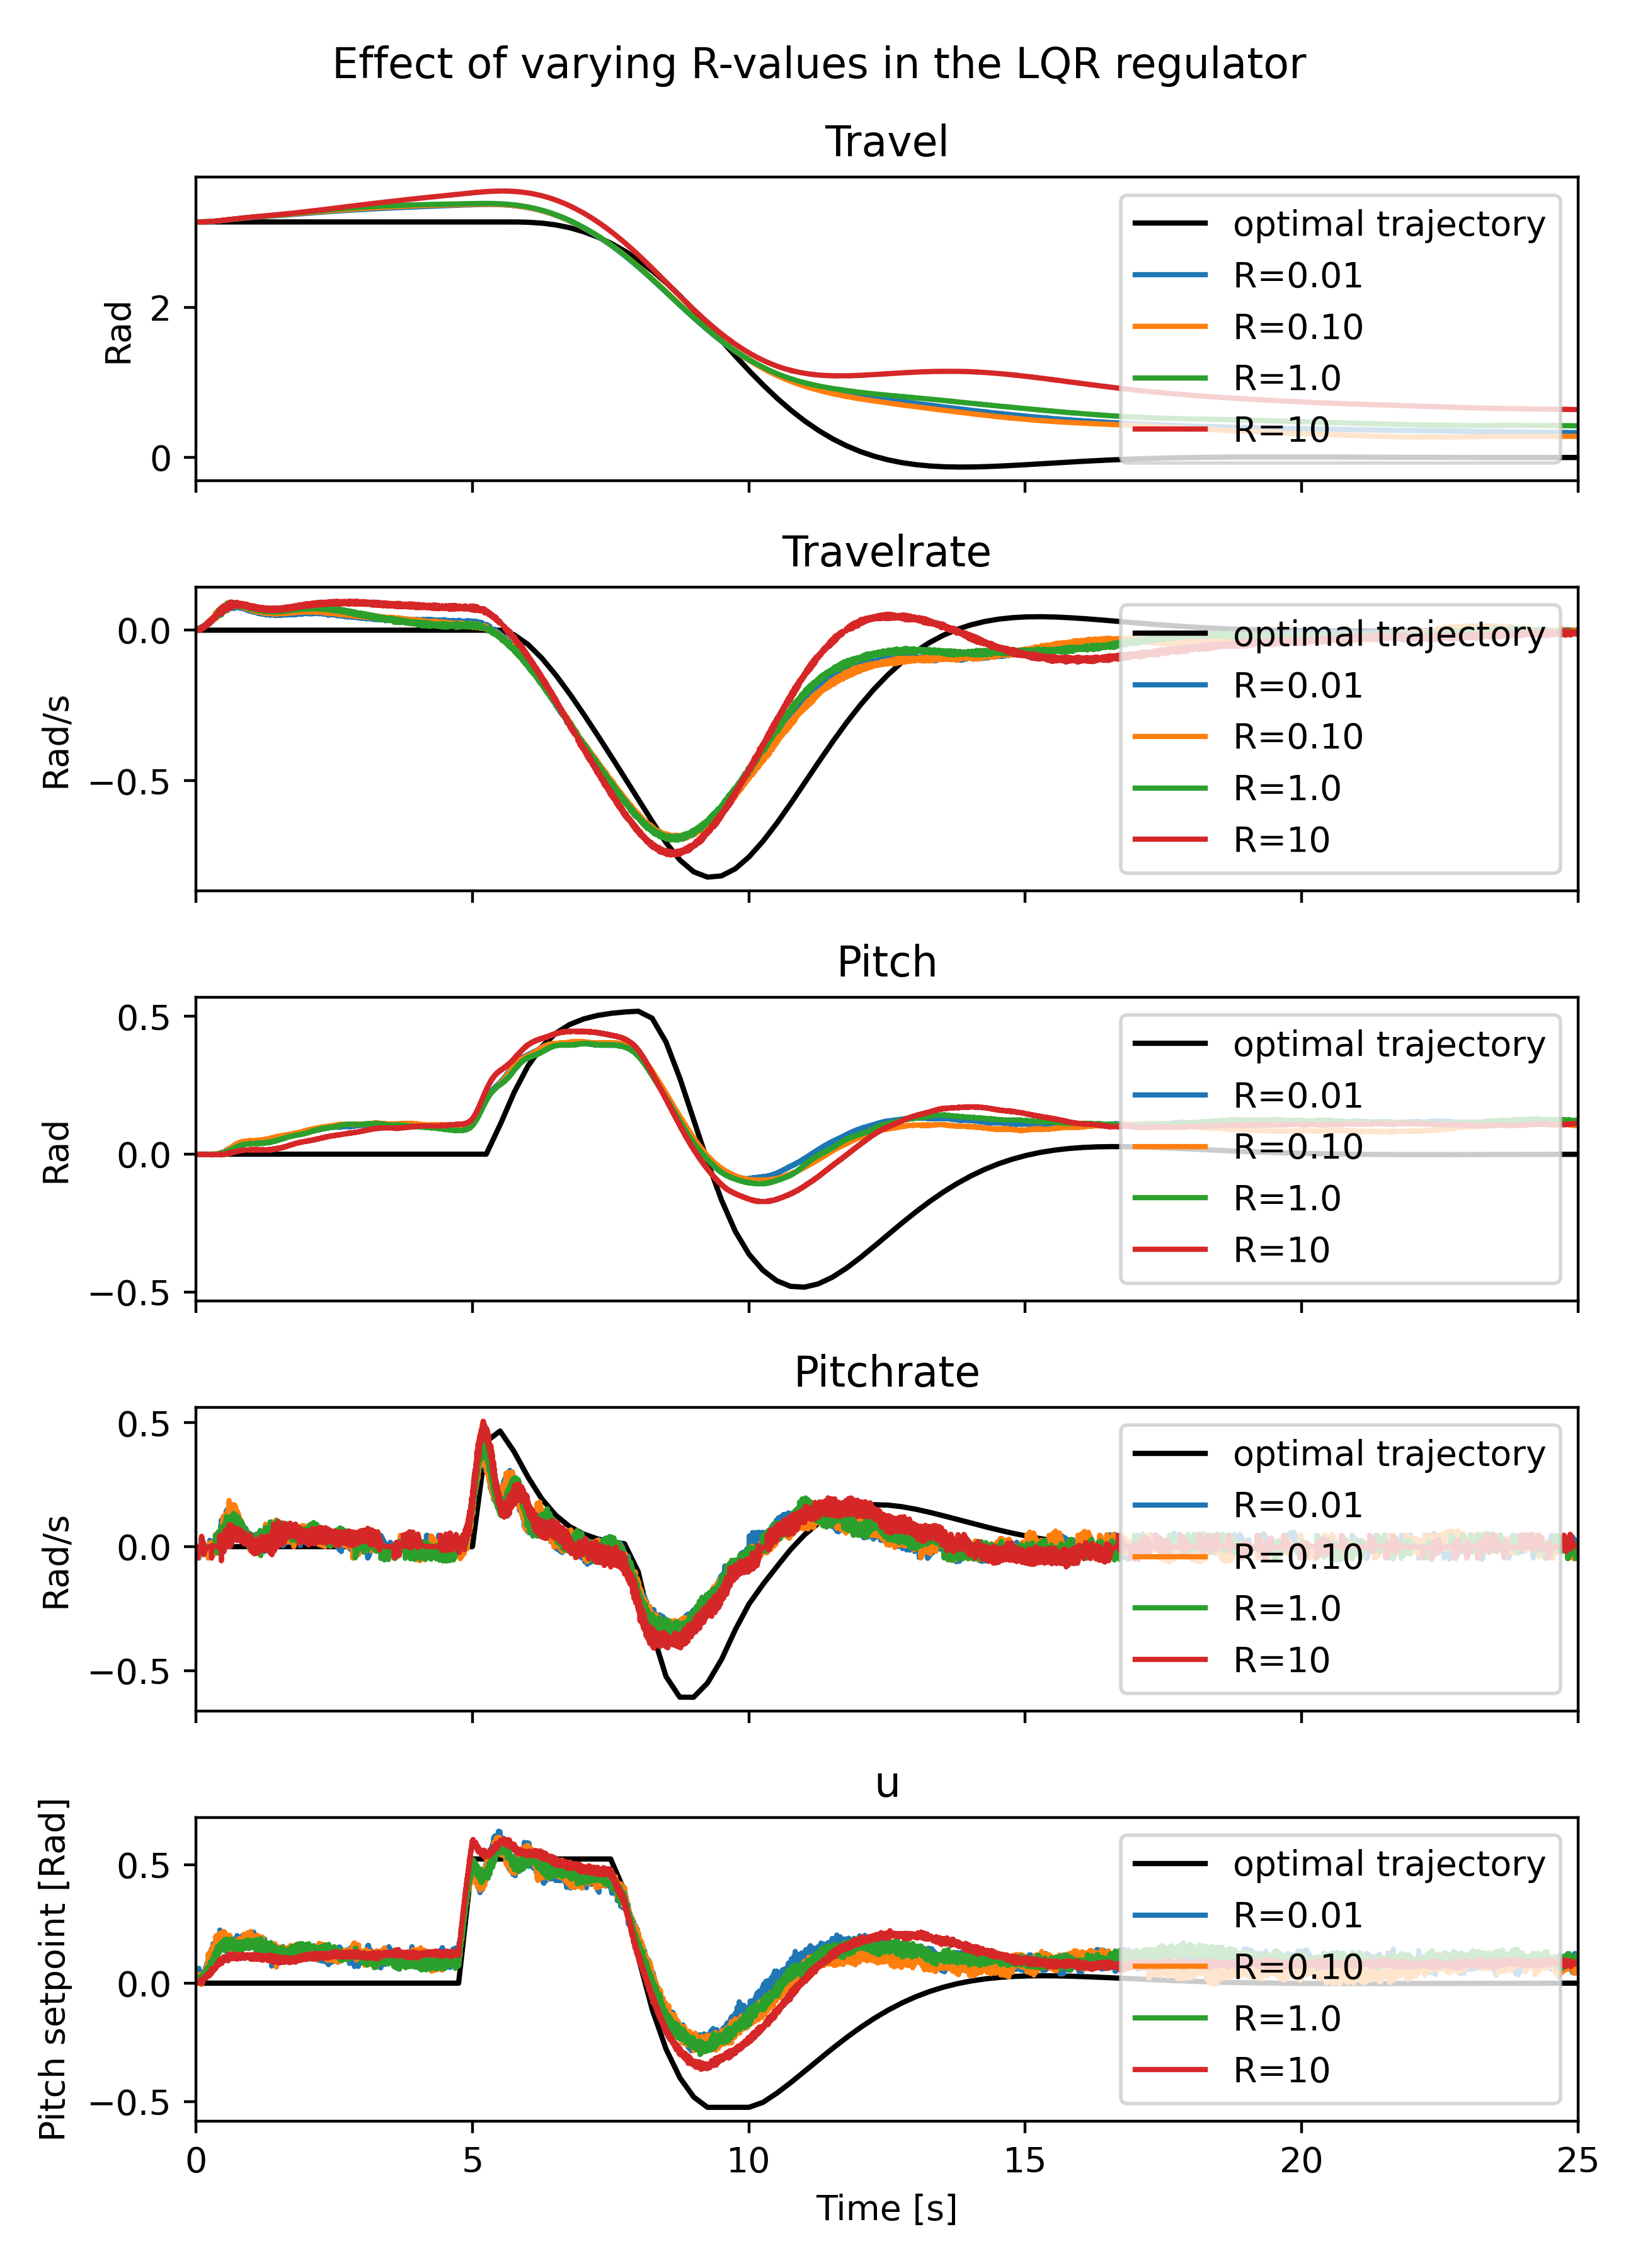
\includegraphics[width=0.8\linewidth]{figures/LAB3_R_variations.png}
	\caption{Prioritizing input-usage while keeping Q=diag([1,1,1,1]). This shows a very slight difference between weights. No further experimentation was done because if $u_k = u_k^*$ then that would be the same as the previous exercise.}
	\label{fig:LAB3_R_variations}
\end{figure}

\begin{figure}[h]
	\centering
	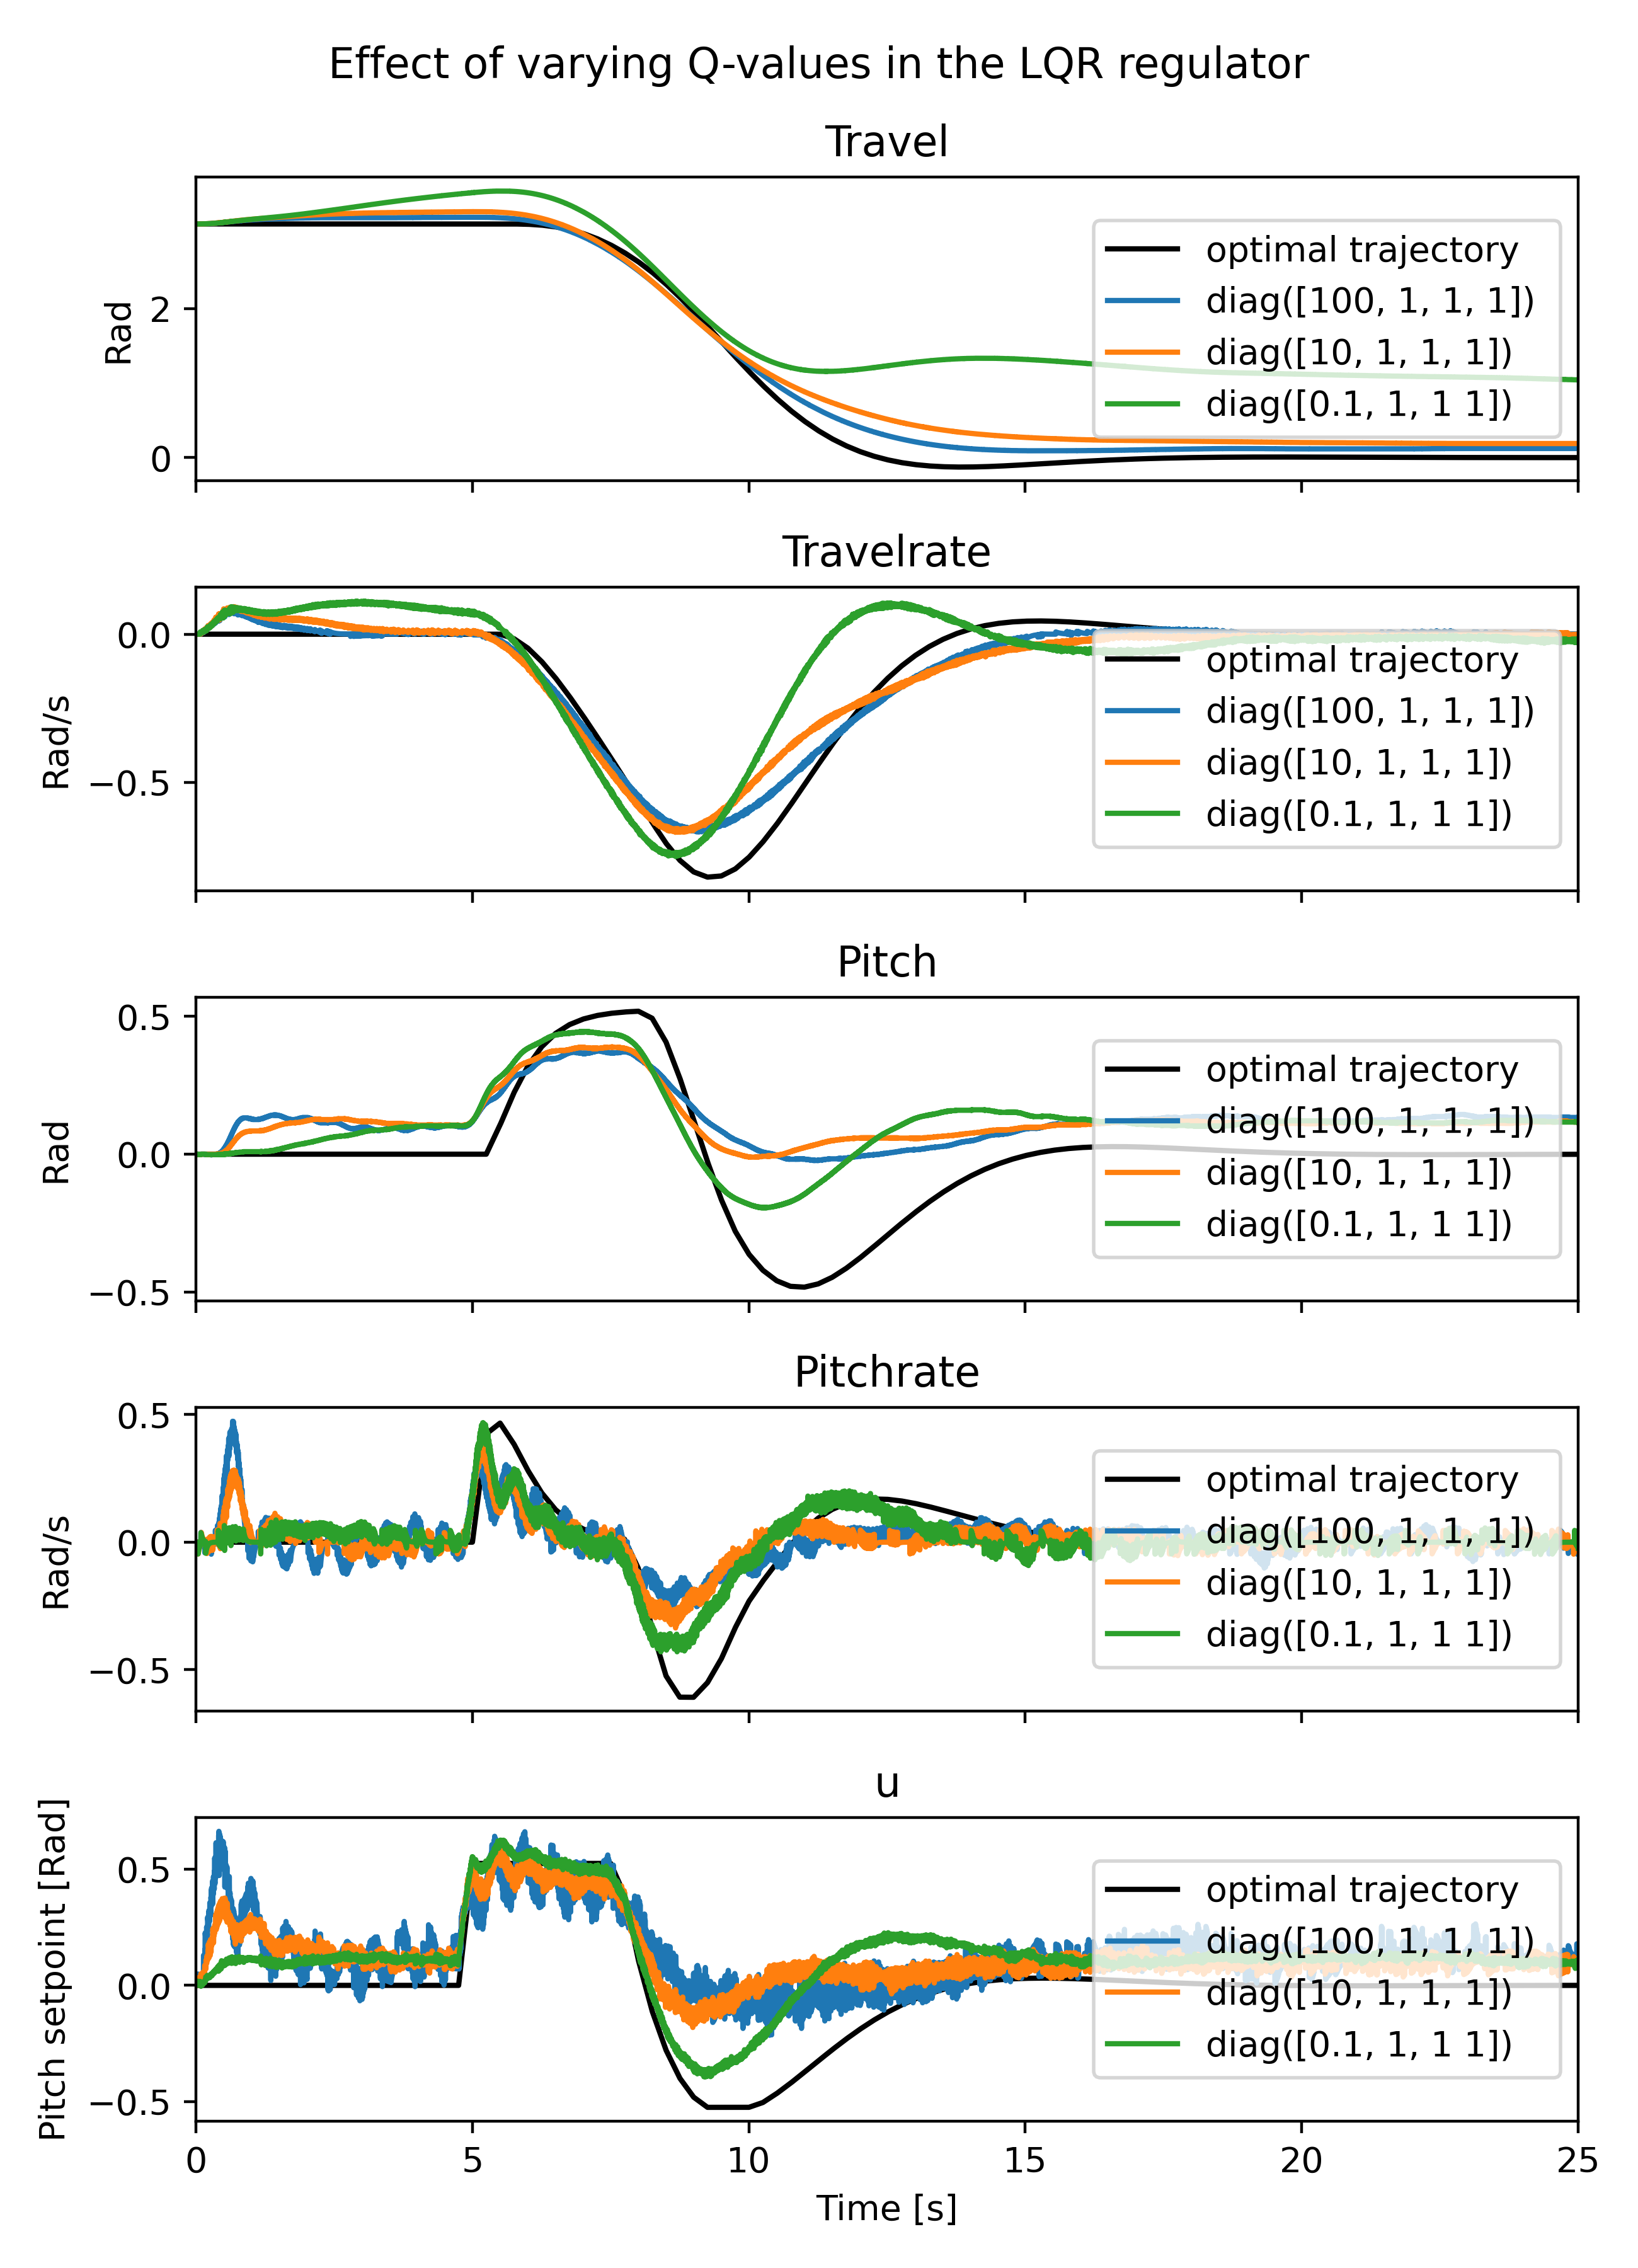
\includegraphics[width=0.8\linewidth]{figures/LAB3_Q_variations.png}
	\caption{Prioritizing the weight related to travel while keeping $R=1$. This was very effective in reducing offset between travel and the planned trajectory. Unfortunately at heigher gains there is some offset introducted and even then there is still a constant offset. A regulator with integral action would probably eliminate this offset without introducting oscillations.}
	\label{fig:LAB3_Q_variations_travel}
\end{figure}

\begin{figure}[h]
	\centering
	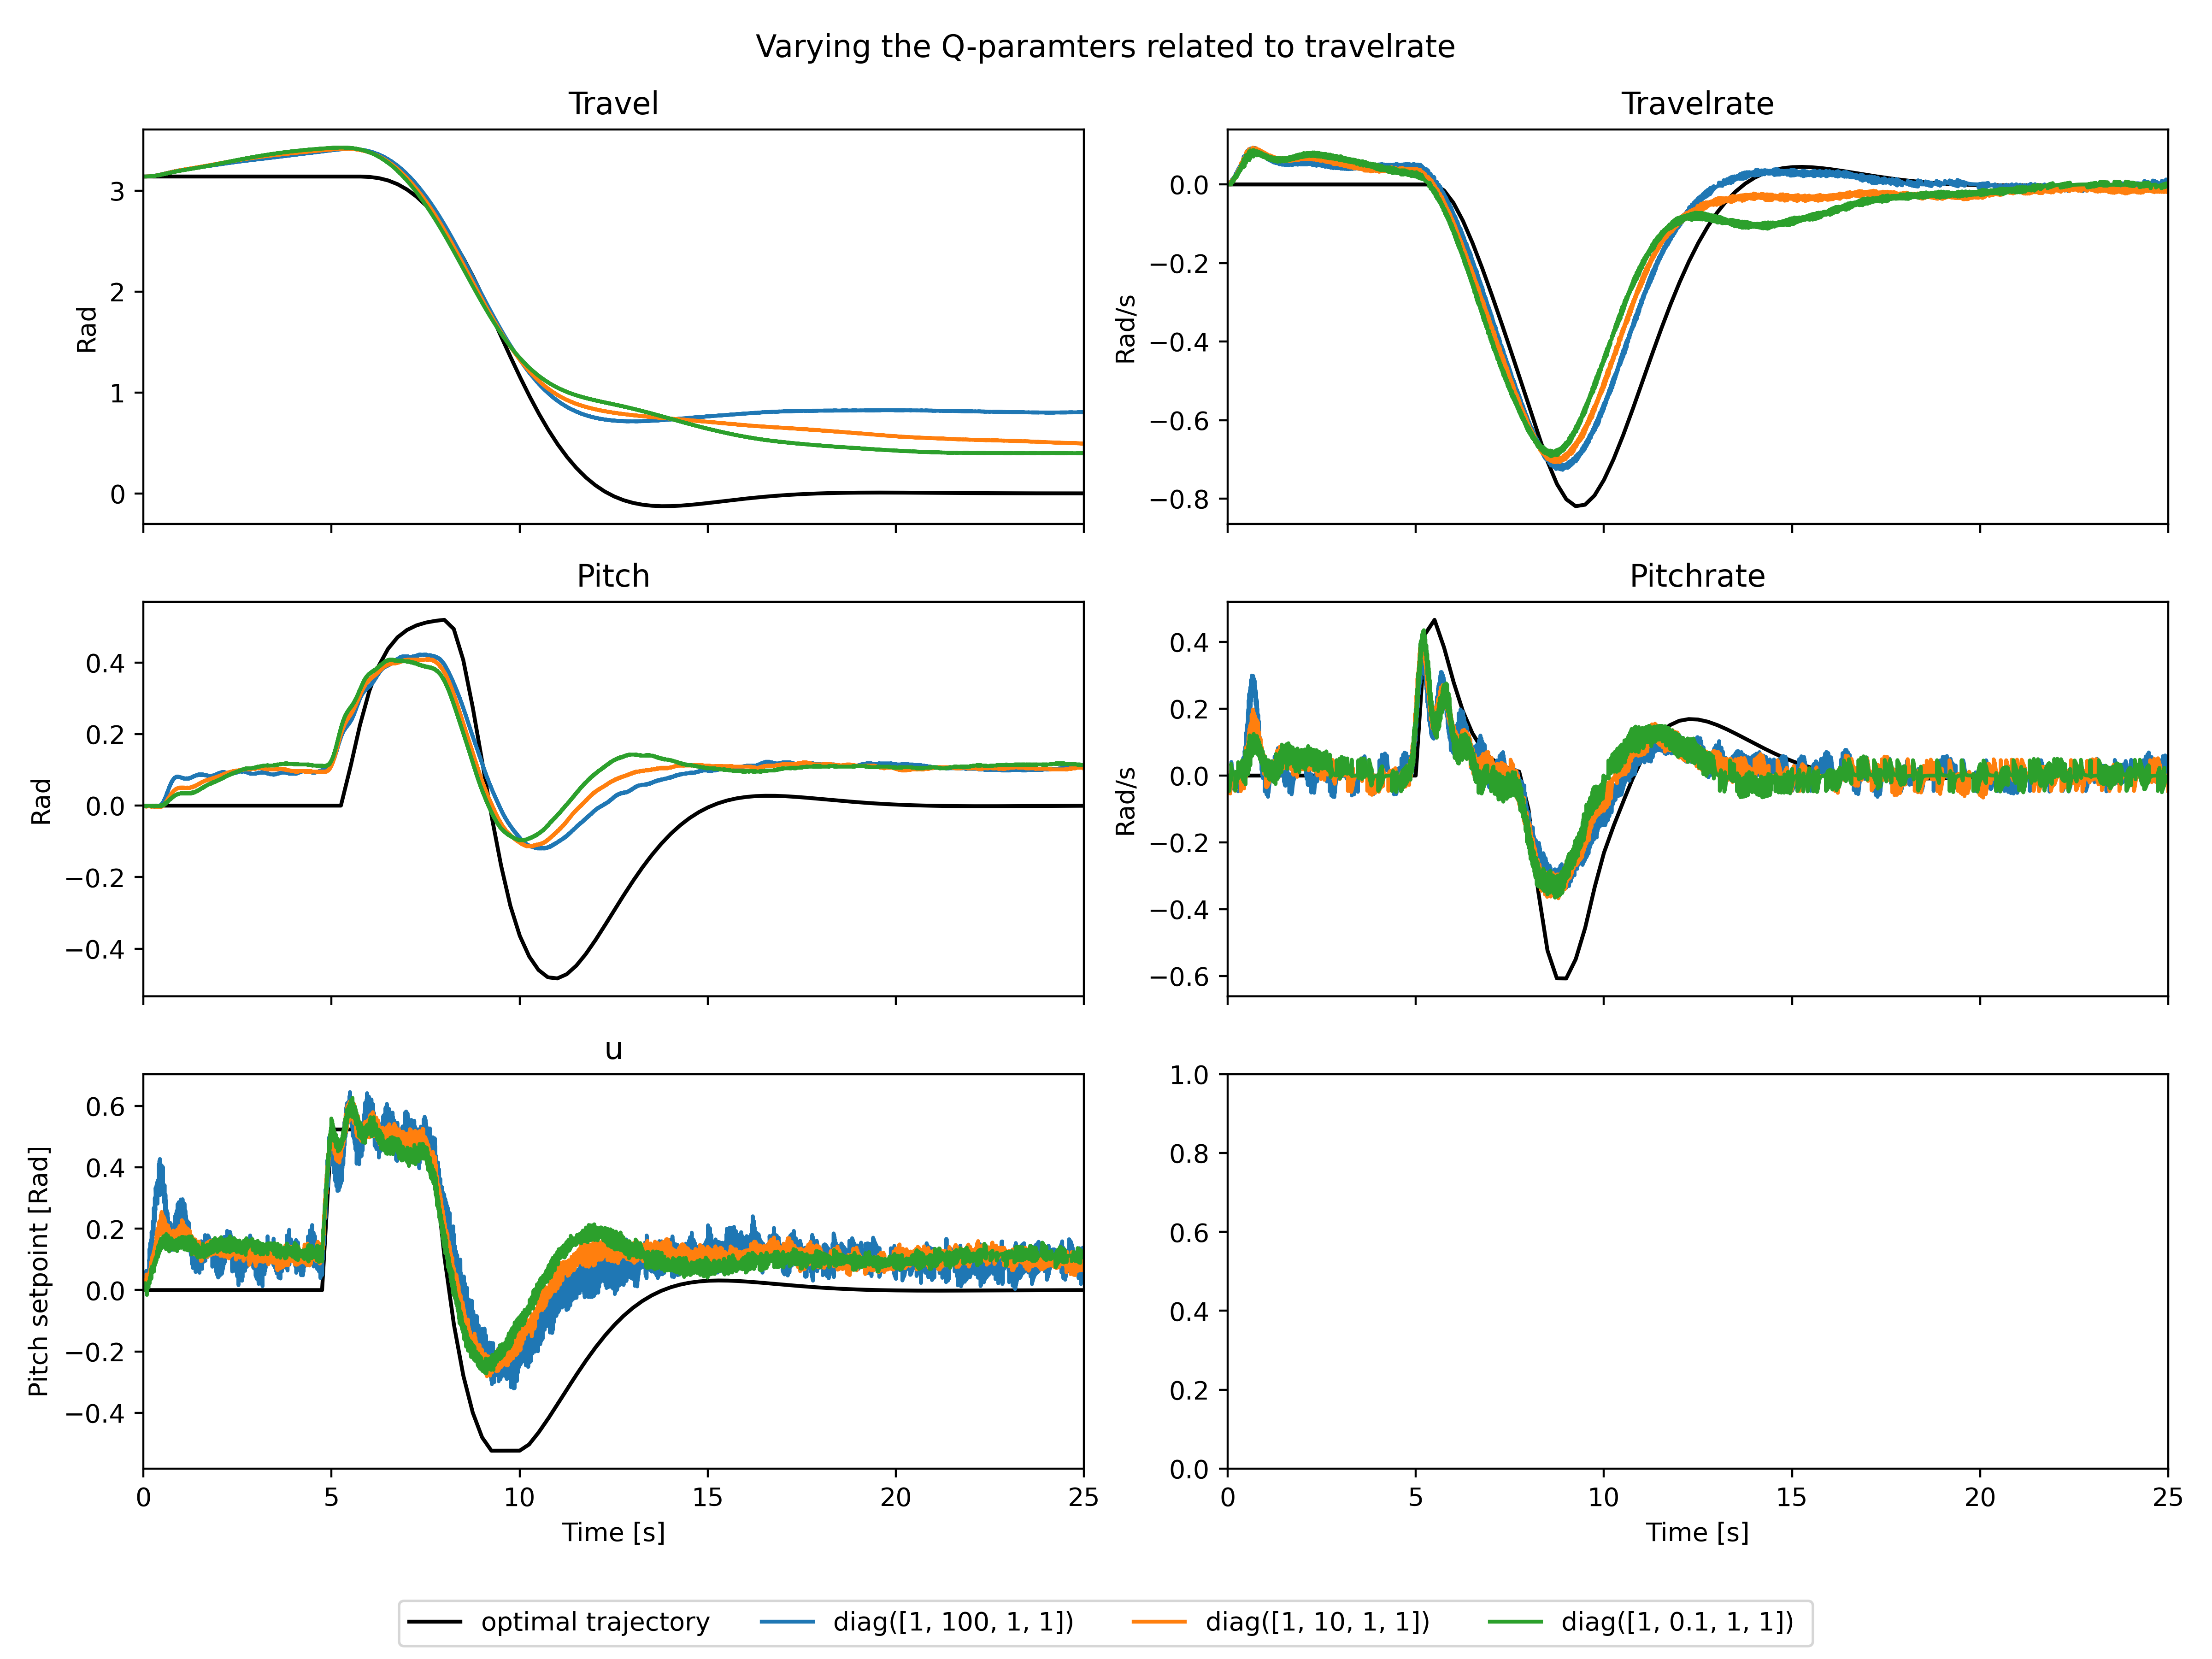
\includegraphics[width=0.8\linewidth]{figures/LAB3_Q_variations_travelrate.png}
	\caption{Changing the weight of the travelrate state, $R=1$. This had only a minor effect with small variations in the response.}
	\label{fig:LAB3_Q_variations_travelrate}
\end{figure}

\begin{figure}[h]
	\centering
	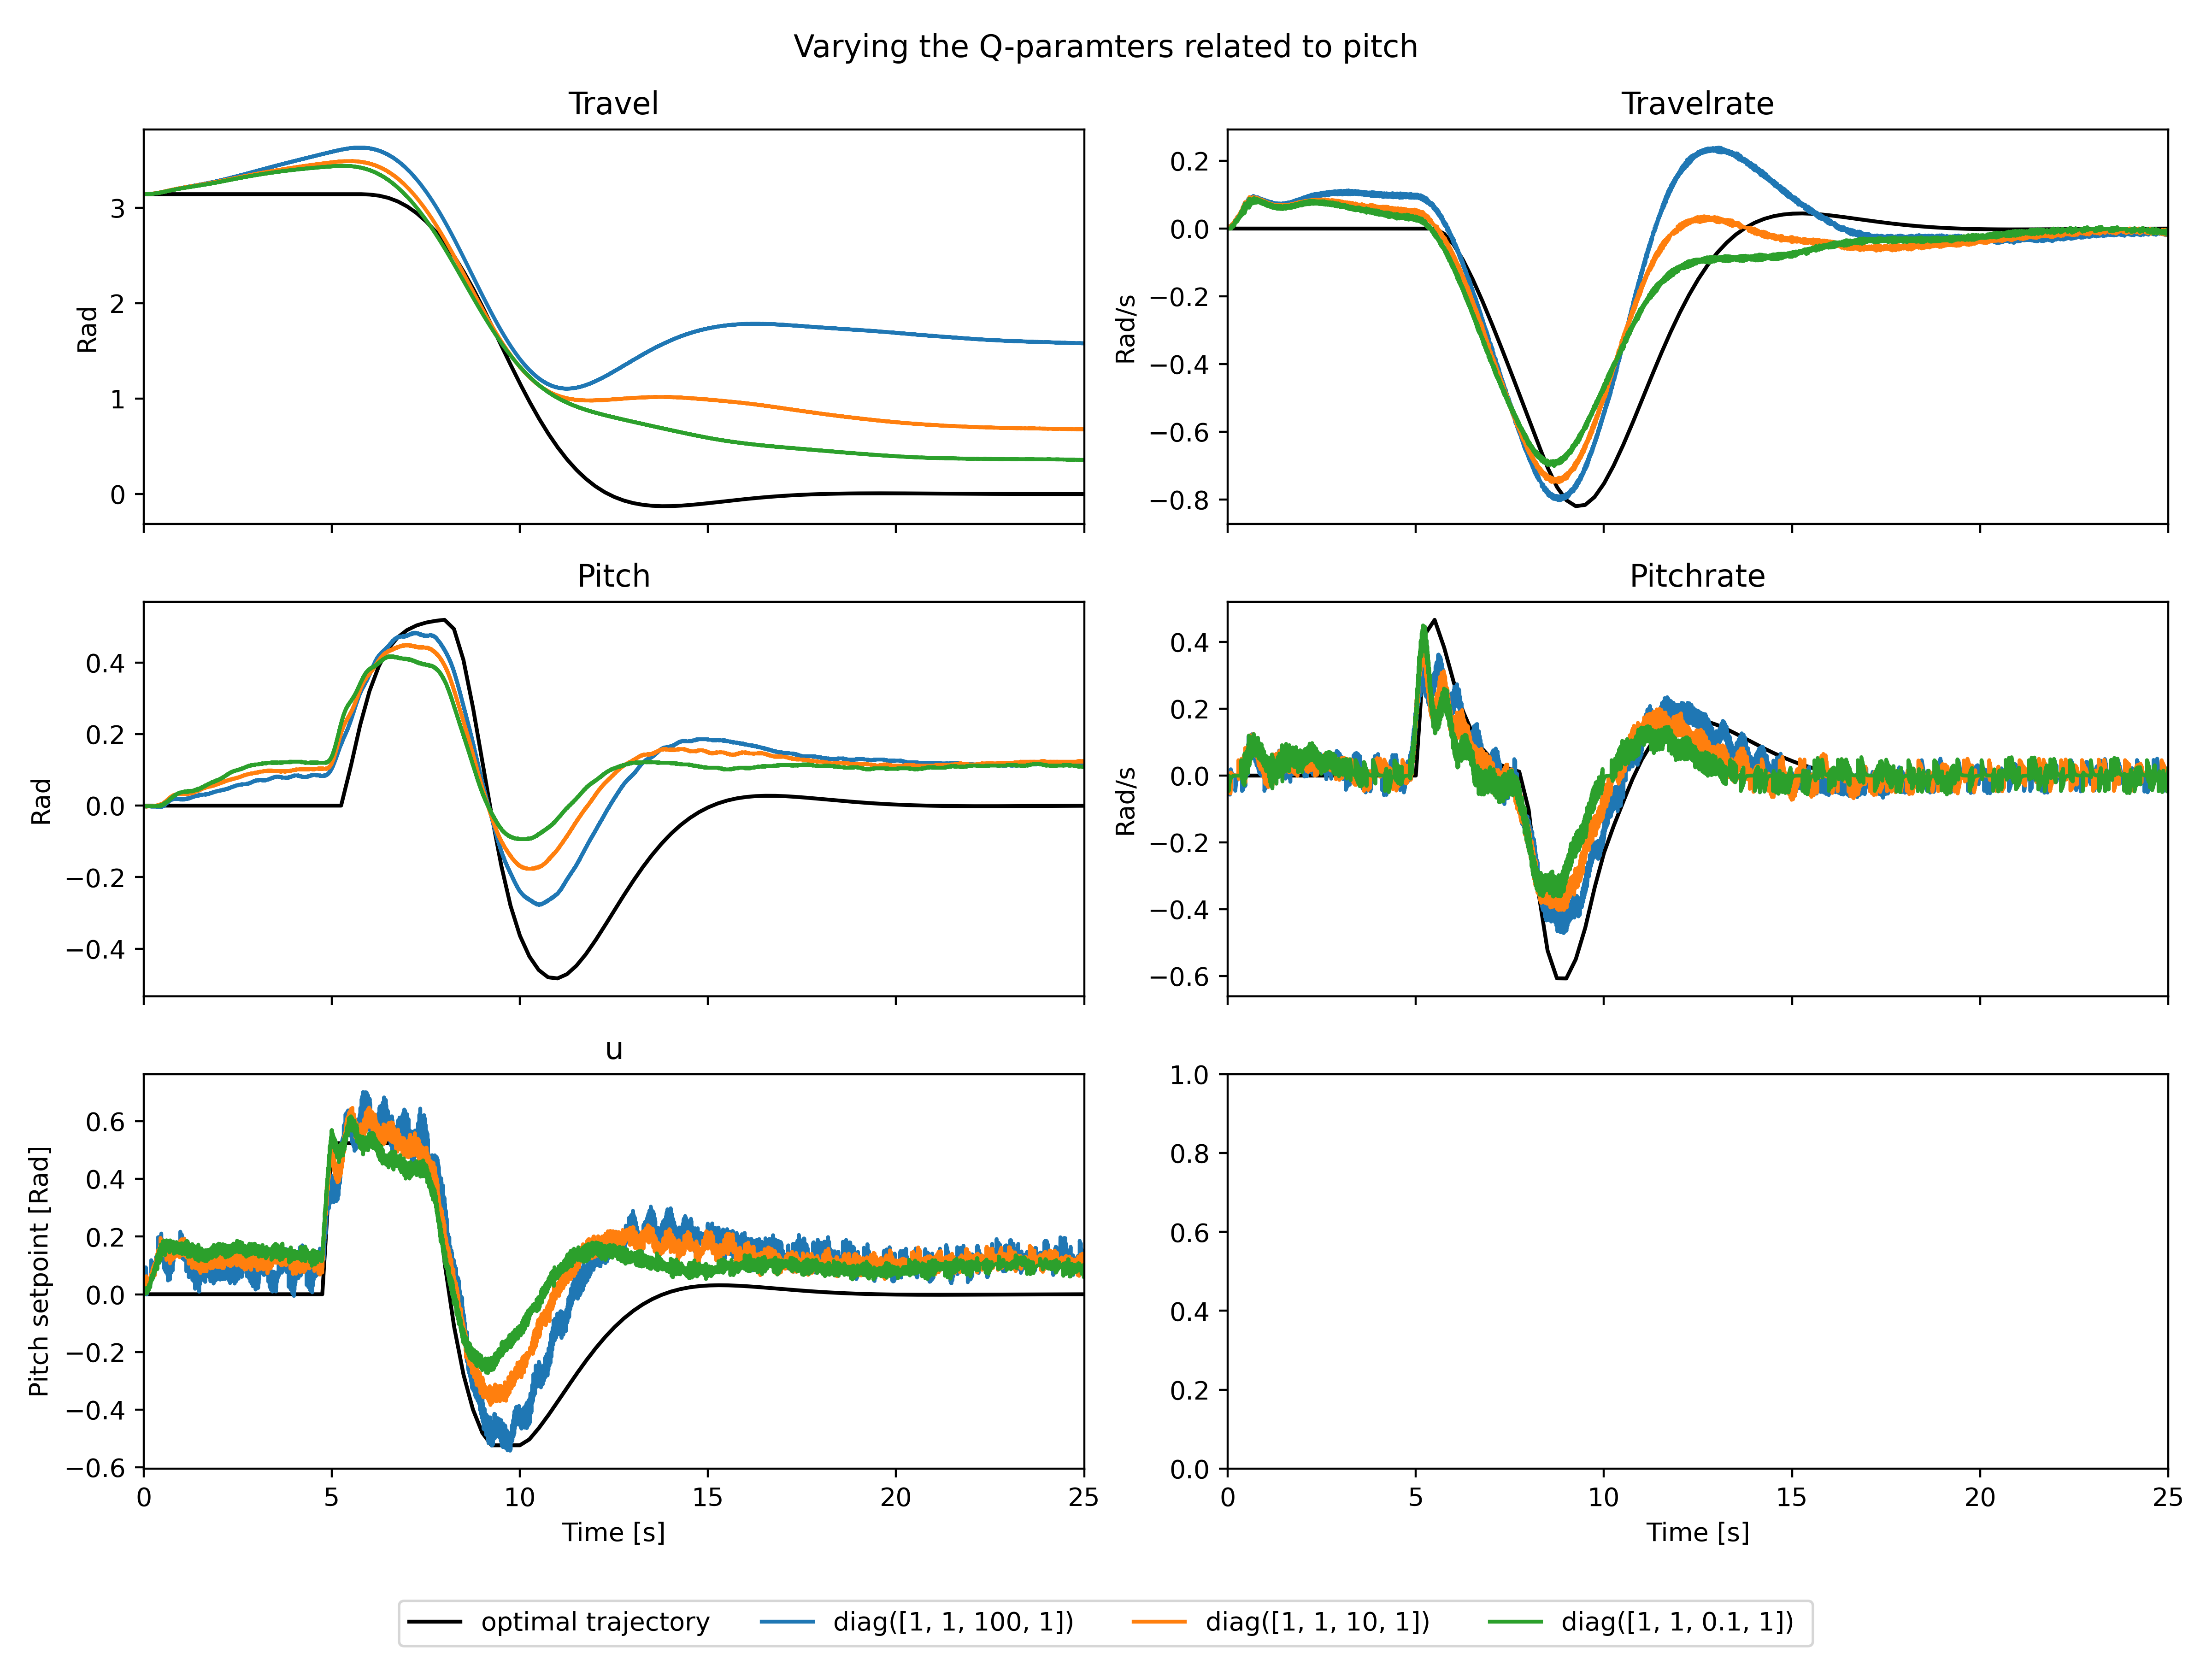
\includegraphics[width=0.8\linewidth]{figures/LAB3_Q_variations_pitch.png}
	\caption{Changing the weight of the pitch state, $R=1$. This had the effect of getting both pitch, pitch-setpoint and pitchrate closer to the planned trajectory at the expense of travel and travelrate.}
	\label{fig:LAB3_Q_variations_pitch}
\end{figure}

\begin{figure}[h]
	\centering
	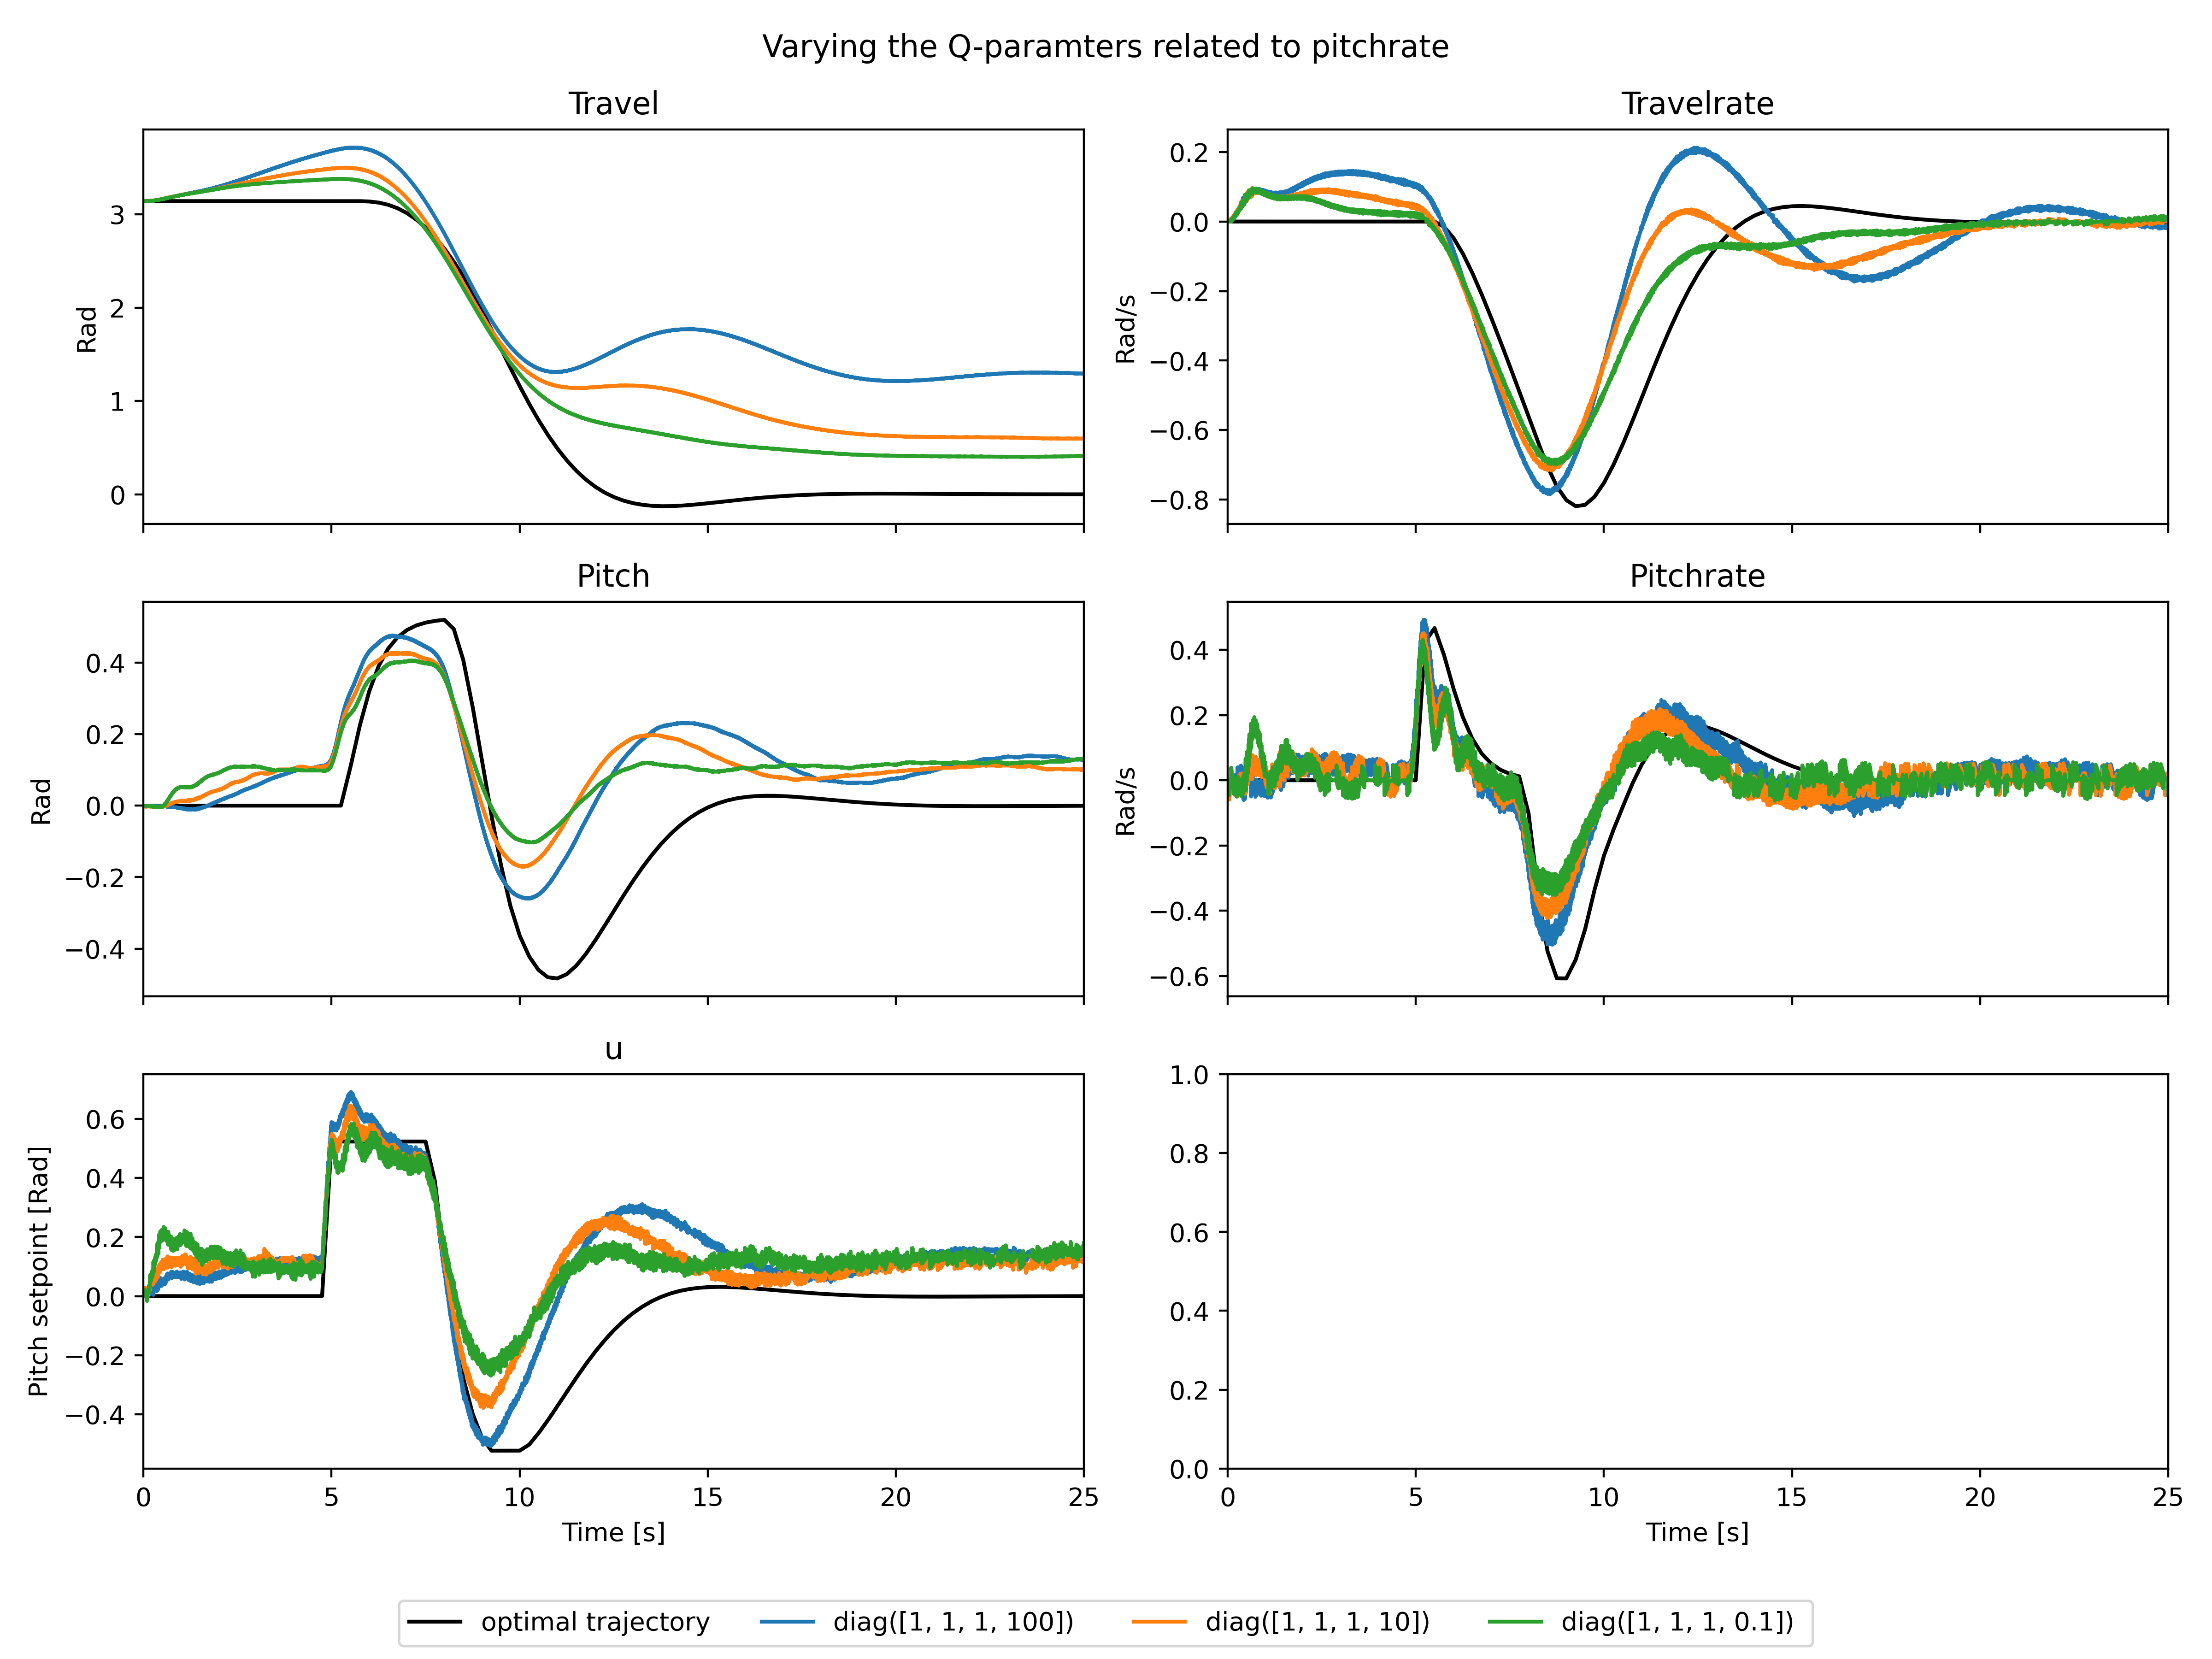
\includegraphics[width=0.8\linewidth]{figures/LAB3_Q_variations_pitchrate.png}
	\caption{Changing the weight of the pitchrate state, $R=1$. This was quite similar to \cref{fig:LAB3_Q_variations_pitch} but there is less oscillation.}
	\label{fig:LAB3_Q_variations_pitchrate}
\end{figure}

\subsubsection{Final tuning}
The final tuning prioritizes travel, as that is the most important state, while comprimizing on the gain - too low results in a large offset while too high results in too much oscillations.

\begin{figure}[h]
	\centering
	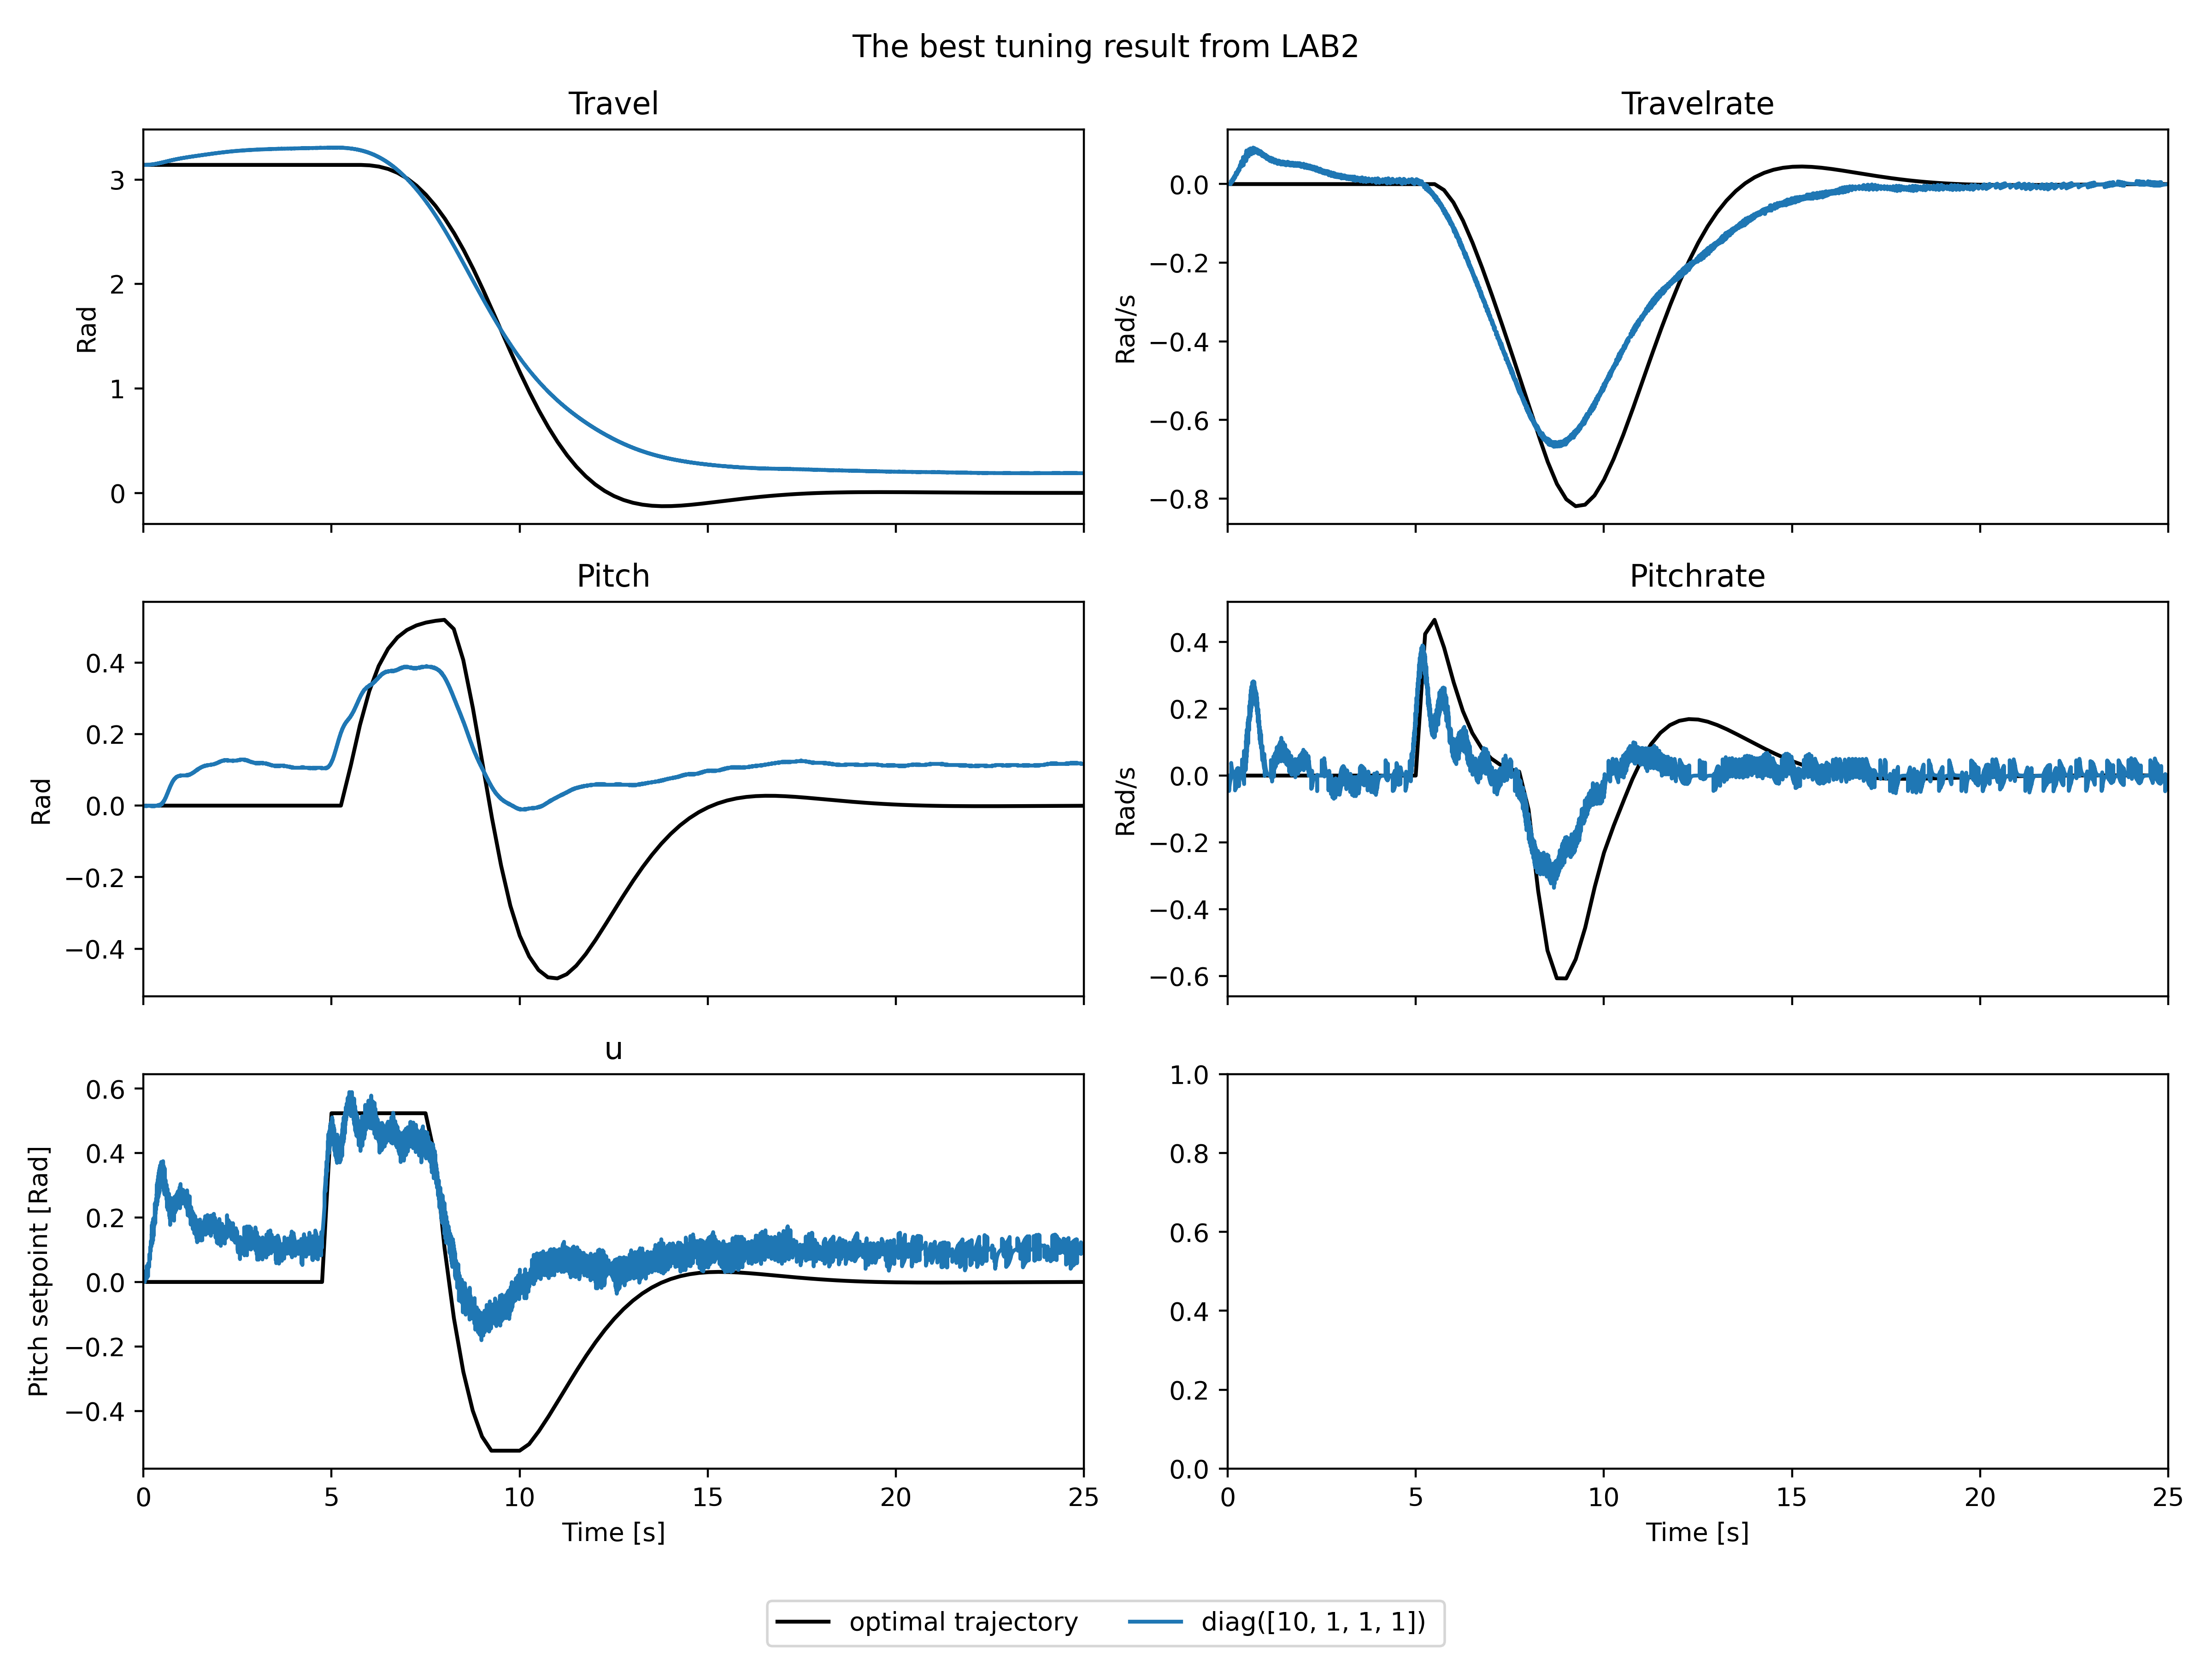
\includegraphics[width=0.8\linewidth]{figures/LAB3_best_tuning.png}
	\caption{The best tuning of LAB3. This tuning prioritizes travel with a good comprimize between high gain and oscillations.}
\end{figure}

\clearpage

\subsection{MATLAB and Simulink}
\lstinputlisting[caption= {MATLAB code for lab 3}, label={lst:lab3_matlab}]{code/problem_3.m}
\subsubsection{Simulink}
\begin{figure}[h]
	\centering
	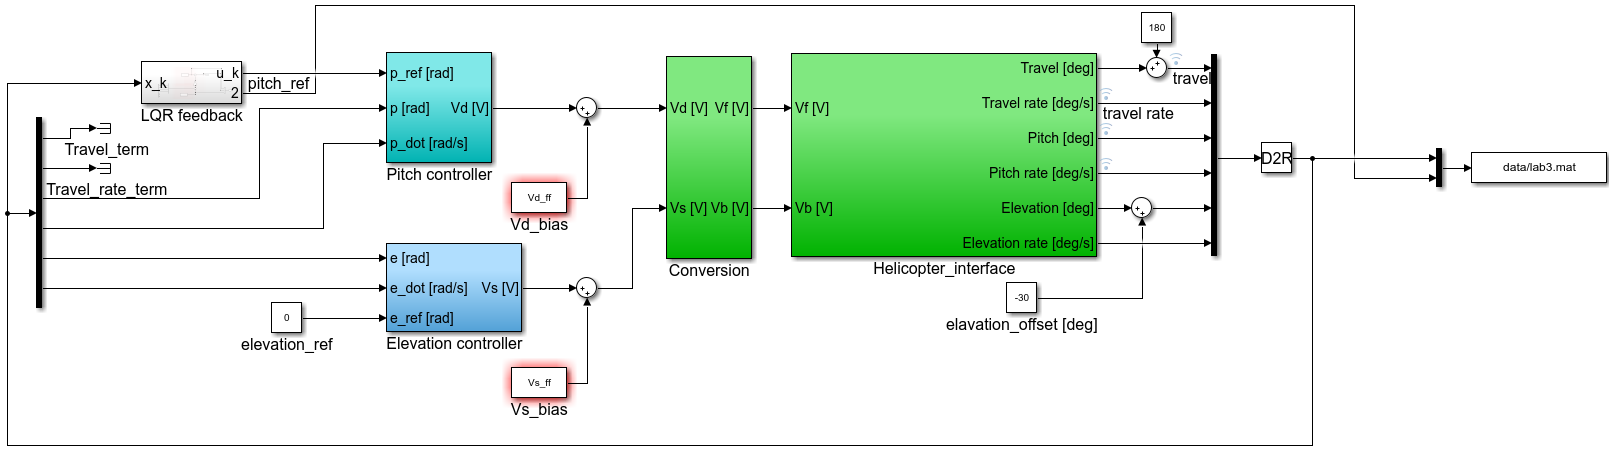
\includegraphics[width=1\linewidth, keepaspectratio]{code/lab3_simulink_1}
	\caption{Simulink diagram used in lab 3.}
	\label{fig:lab3_simulink}
\end{figure}
\begin{figure}[h]
	\centering
	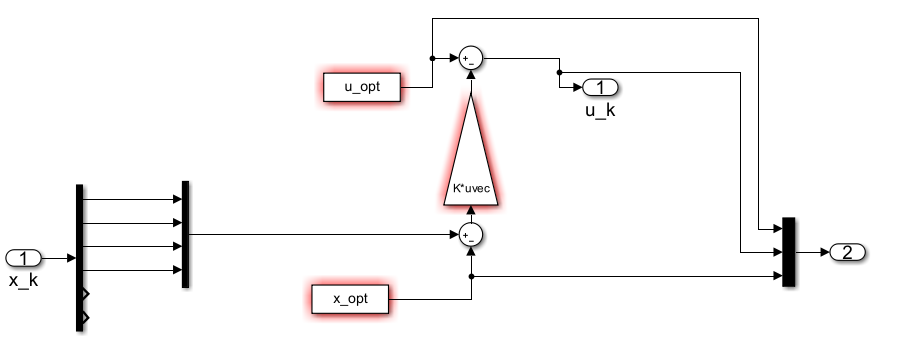
\includegraphics[width=1\linewidth, keepaspectratio]{code/lab3_simulink_2}
	\caption{``LQR Feedback'' subsystem in \cref{fig:lab3_simulink}}
	\label{fig:lab3_simulink_lqr}
\end{figure}
\end{document}
\documentclass[../main.tex]{subfiles}

\begin{document}
\section{10.4 - Optimal Control of Pitch/Travel and Elevation with Feedback}
In the previous labs the elevation has been disregarded, and assumed to be zero. In this lab, elevation is not disregarded, and the group had to calculate an optimal trajectory for the elevation as well. The criteria to be minimized was
\begin{equation}\label{eq:lab4_cost_func}
	\phi = \sum_{i=0}^{N-1} (\lambda_{i + 1} - \lambda_f)^{2} + q_1 p_{ci}^2 + q_2 e_{ci} ^2
\end{equation}
and the constraint on the elevation was:
\begin{equation}\label{eq:lab4_elevation_constraint}
	e_k \geq \alpha \text{exp}\left( -\beta (\lambda_k - \lambda_t)^2\right) \forall k \in \left\lbrace 1,...,N\right\rbrace 
\end{equation}

\subsection{The continuous model}
\textit{Answer 10.4.1.1}
The equation for elevation has been given in the problem description as
\begin{equation}\label{eq:lab4_elevation}
	\ddot{e} + K_3K_{ed}\dot{e} + K_3K_{ep}e = K_3K_{ep}e_c
\end{equation}
where $ e_c $ is the elevation setpoint.

Expanding the system defined in \cref{eq:lab2_cont_ss} to include \cref{eq:lab4_elevation}, gives a new system that includes the elevation:

\begin{equation}\label{eq:lab4_cont_ss}
	\underbrace{\begin{bmatrix}
			\dot \lambda \\
			\dot r \\
			\dot p \\
			\ddot p \\
			\dot e \\
			\ddot e \\
	\end{bmatrix}}_{\bm{\dot x}} = 
	\underbrace{
		\begin{bmatrix}
			0 & 1 & 0 & 0 & 0 & 0\\
			0 & 0 & -K_2 & 0 & 0 & 0\\
			0 & 0 & 0 & 1 & 0 & 0\\
			0 & 0 & -K_1 K_{pp} &  -K_1 K_{pd} & 0 & 0\\
			0 & 0 & 0 & 0 & 0 & 1 \\
			0 & 0 & 0 & 0 & -K_3K_{ep} & -K_3K_{ed} \\
		\end{bmatrix}
	}_{\bm A_c}
	\underbrace{
		\begin{bmatrix}
			\lambda \\ r \\ p \\ \dot{p} \\ e \\ \dot{e}
		\end{bmatrix}
	}_{\bm x}
	+
	\underbrace{
		\begin{bmatrix}
			0 & 0 \\
			0 & 0\\
			0 & 0\\
			K_1 K_{pp} & 0\\
			0 & 0 \\
			0 & K_3K_{ep} \\
		\end{bmatrix}
	}_{\bm B_c} 
	\underbrace{
		\begin{bmatrix}
			p_c \\
			e_c \\
		\end{bmatrix}
	}_{\bm u}
\end{equation}

\subsection{The discretized model}
\textit{Answer 10.4.1.2}
Discretizing the continuous system defined in \cref{eq:lab4_cont_ss} was done using the forward Euler method (see \cref{sec:lab2_disc} for more information about this method).

The resulting dicretized system became: 
\begin{equation}\label{eq:lab4_disc_ss}
	\bm A_d = \begin{bmatrix}
		1 & T & 0 & 0 & 0 & 0\\
		0 & 1 & -TK_2 & 0 & 0 & 0\\
		0 & 0 & 1 & T & 0 & 0\\
		0 & 0 & -T K_1 K_{pp} &  1 - T K_1 K_{pd} & 0 & 0\\
		0 & 0 & 0 & 0 & 1 & T \\
		0 & 0 & 0 & 0 & -T K_3 K_{ep} & 1 - TK_3K_{ed} \\
	\end{bmatrix}, \quad
	\bm B_d = \begin{bmatrix}
		0 & 0 \\
		0 & 0\\
		0 & 0\\
		T K_1 K_{pp} & 0\\
		0 & 0 \\
		0 & T K_3K_{ep} \\
	\end{bmatrix}
\end{equation}
where $ T $ is the sample-time.

\subsection{Experimental results}
\textit{Printouts of data from relevant experiments (plots).
Discussion and analysis of the results.
Answer 10.4.2.6 here.}

The group's goal was as in the other labs, to make the helicopter follow the optimal trajectory to $ \lambda_f $ as close as possible. Making the helicopter follow the trajectory consisted of two parts: 
\begin{enumerate}
	\item Tune the LQ regulator to get a good feedback-gain matrix.
	\item Find an optimal trajectory the helicopter could follow.
\end{enumerate}

\subsubsection{Tuning LQ regulator}
Before the group started testing the helicopter's response optimal trajectory found using the SQP-algorithm, the LQ regulator used to find the feedback-gain matrix $\bm K$ had to be tuned. The LQ regulator was exactly the same as the one describe in \cref{kap:task_10_3_LQ_controller}, but now with expanded state and input as described in \cref{eq:lab4_cont_ss}. This means that $ \bm Q $ was now a diagonal matrix of size 6x6, and $ \bm R $ was a diagonal matrix of 2x2. Tuning the LQ regulator is a vital part of achieving as good response. Since the elevation is decoupled from the rest of the states, it should been possible to use the tuning from \cref{sec:lab3_result} and find a good tuning for the elevation (i.e. tuning Q(5,5), Q(6,6) and R(2, 2)). However, in reality the helicopter's state is not decoupled (see \cref{sec:lab4_decoupled}), so to achieve good tuning the group had to tune the whole system again.

A good rule of thumb is that the LQ regulator should be tuned with an input trajectory that one know the helicopter actually can follow. If the helicopter has an input trajectory that is physical impossible to achieve, the tuning will become hard. Therefore, the group tried to create a moderate input-trajectory which seemed reasonable based on their experience from the lab. However, the task was harder than anticipated, and the group did not have enough time to do this. 

Since the group was not able to make a tuning-trajectory for the states and inputs, an optimal trajectory from solving the optimization problem using $q_1 = q_2 = 1$ in the cost function, was used as a replacement. This gave the optimal trajectories shown in \cref{fig:lab4_opt_trajectory}

\begin{figure}[h]
	\centering
	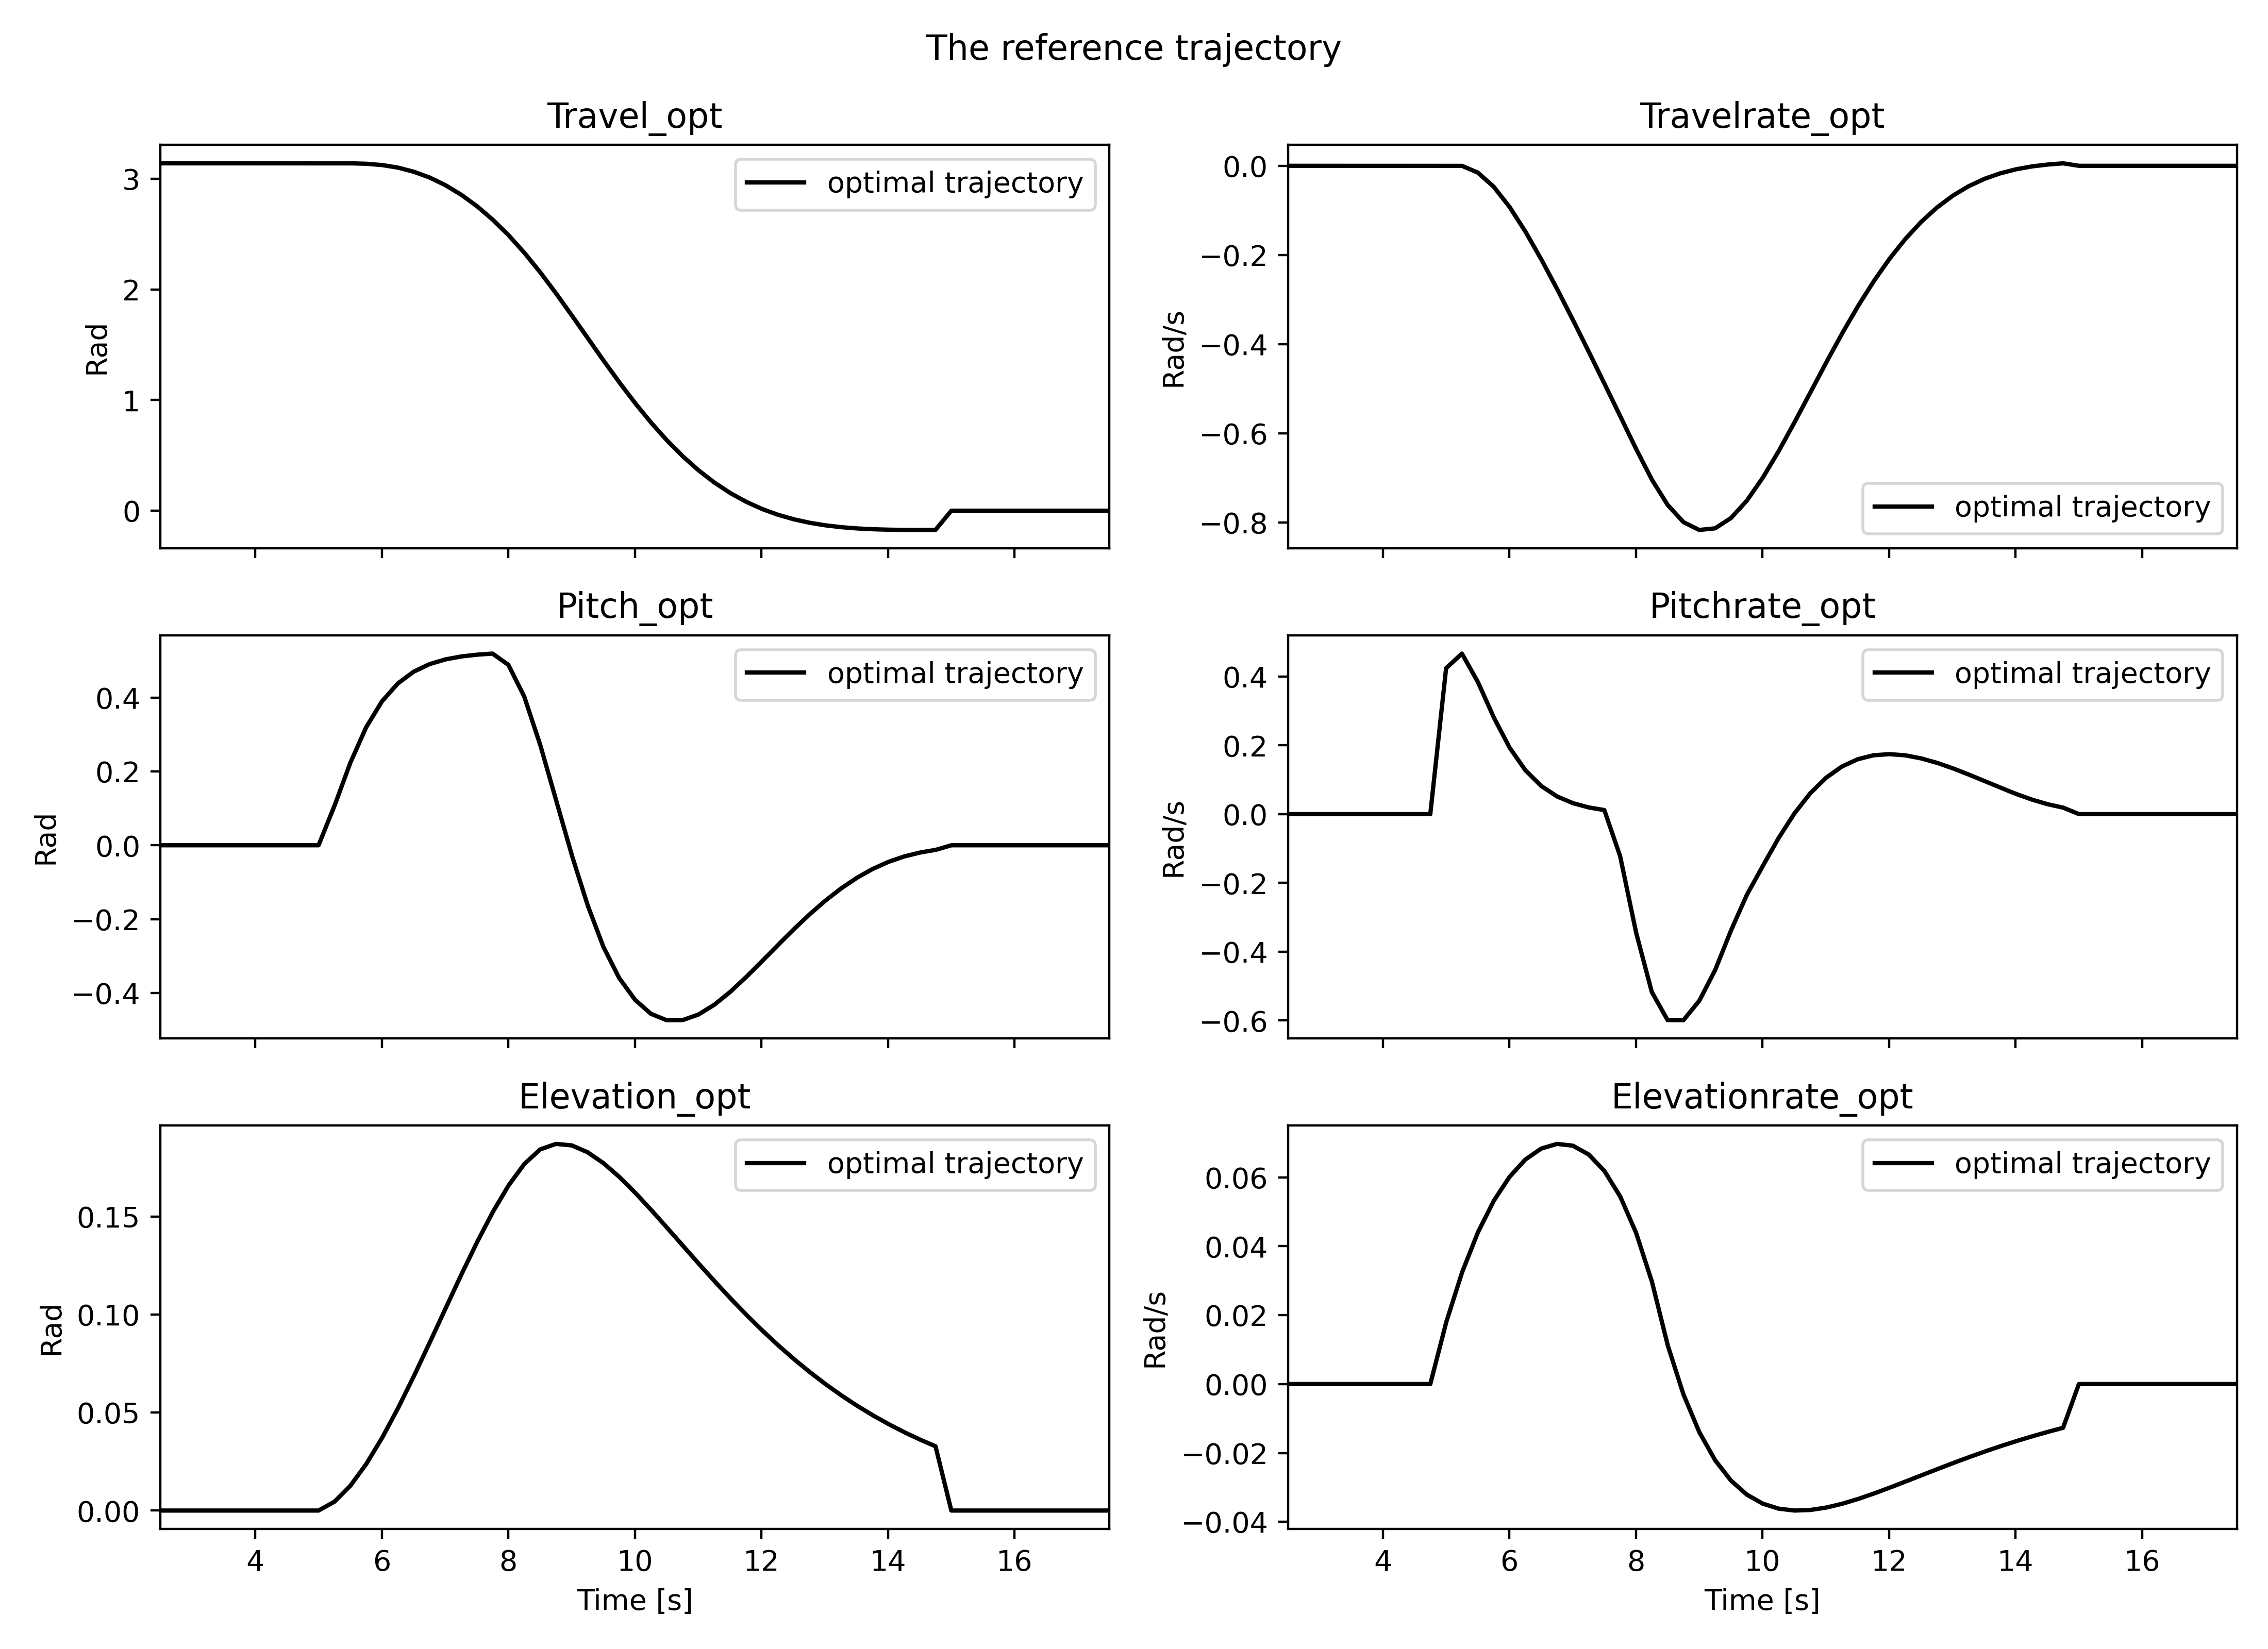
\includegraphics[width=\linewidth]{figures/LAB4_reference_trajectory.png}
	\caption{Optimal trajectories using  $q_1 = q_2 = 1$ in the cost function.}
\end{figure}

In the tuning process we decided to keep $ \bm R $ and $ \bm Q $ as diagonal matrices. $ \bm R $ was set constant equal the identity matrix, i.e. $\bm R = \bm I_2$. The diagonal elements of $ \bm Q $ was then changed to get a good tuning. As in \todo{cref lab3 lqr tuning}each diagonal entry in Q corresponds to the corresponding state in \cref{eq:lab4_cont_ss} \todo{REFORMULATE}. This makes the tuning process simpler since a change in an entry $ \bm Q $ has an expected impact on the response. Higher values of $ \bm Q $ results in inputs with larger magnitude, which again gives a faster response. Having too small values on the diagonal of $ \bm Q $ will therefor give a slow response. Having too large values on the diagonal of $ \bm Q $ will also have unwanted effects as the helicopter approaches a less stable tuning. This is shown in \cref{fig:lab4_diff_Q_values} where the low valued $ \bm Q $ gives a slower response, and a higher valued $ \bm Q $ gives an oscillating response (especially for the pitch rate). The oscillations are noticeable in th ereal world as a shaking helicopter.
\begin{figure}[h]
	\centering
	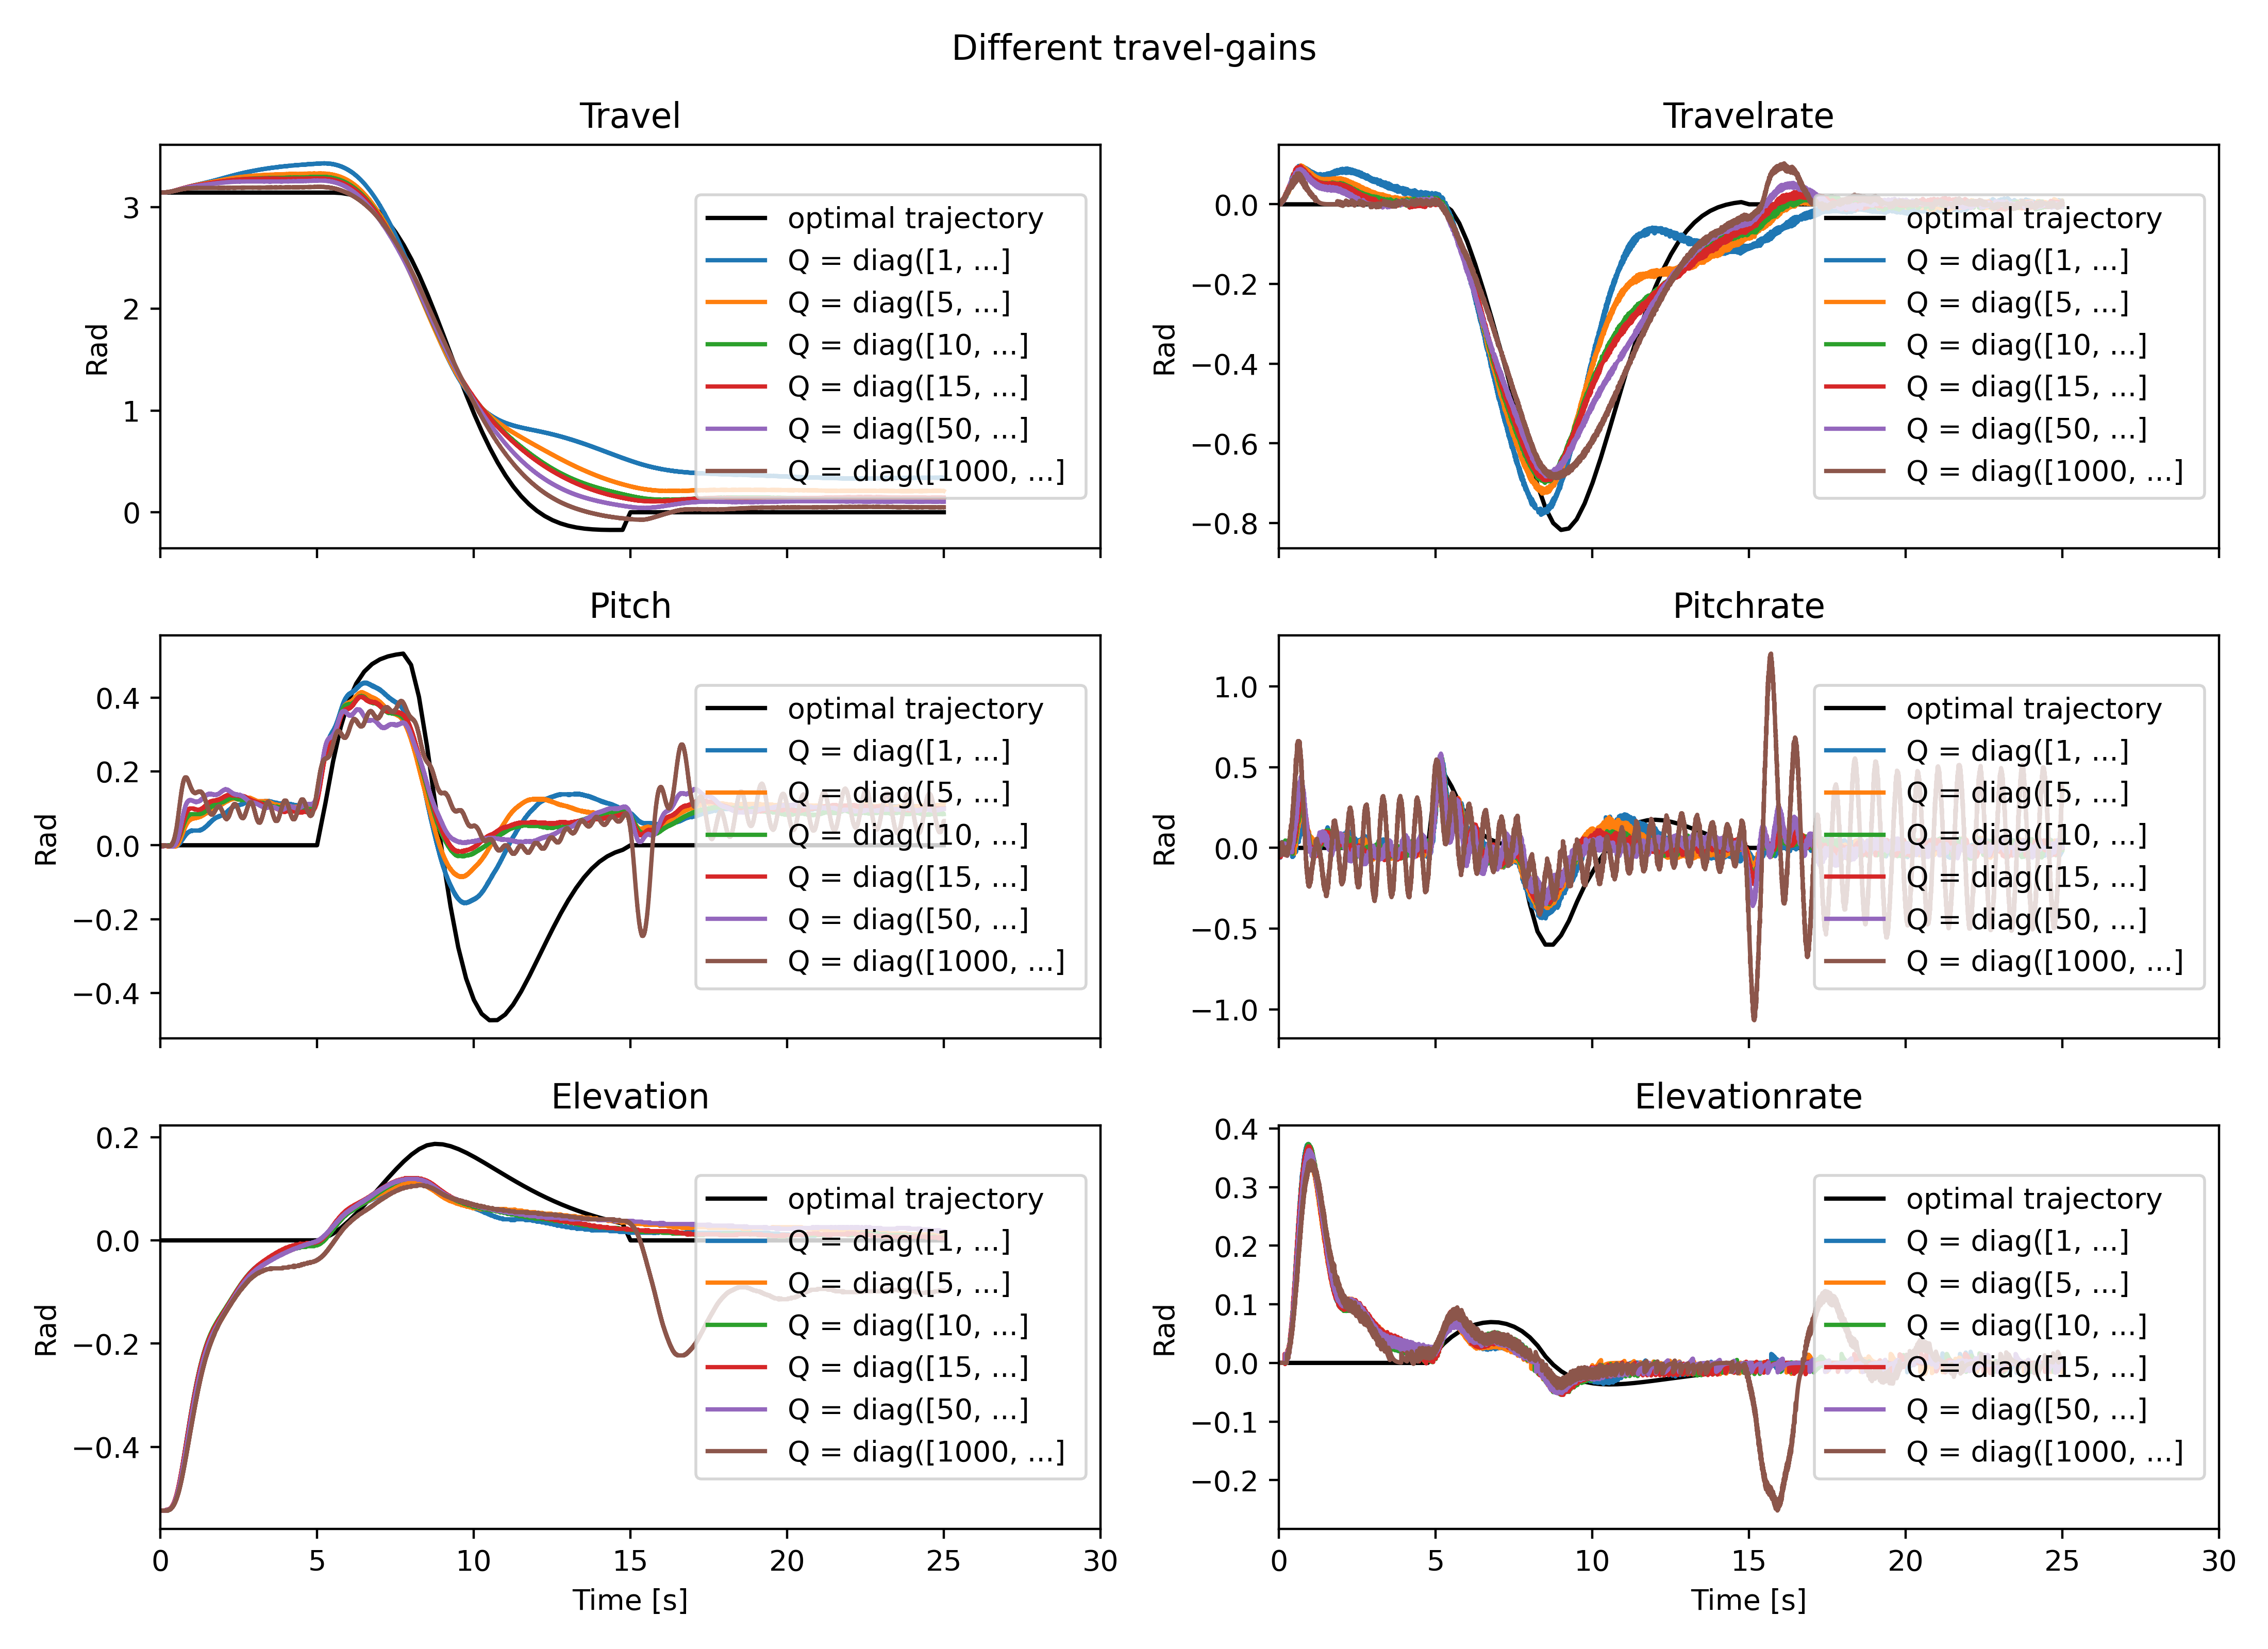
\includegraphics[width=\linewidth]{figures/LAB4_travel_gains.png}
	\caption{Her er alle verdiene vi brukte, bør nok rydde opp litt.}
	\label{fig:lab4_diff_Q_values}
\end{figure}

\begin{figure}[h]
	\centering
	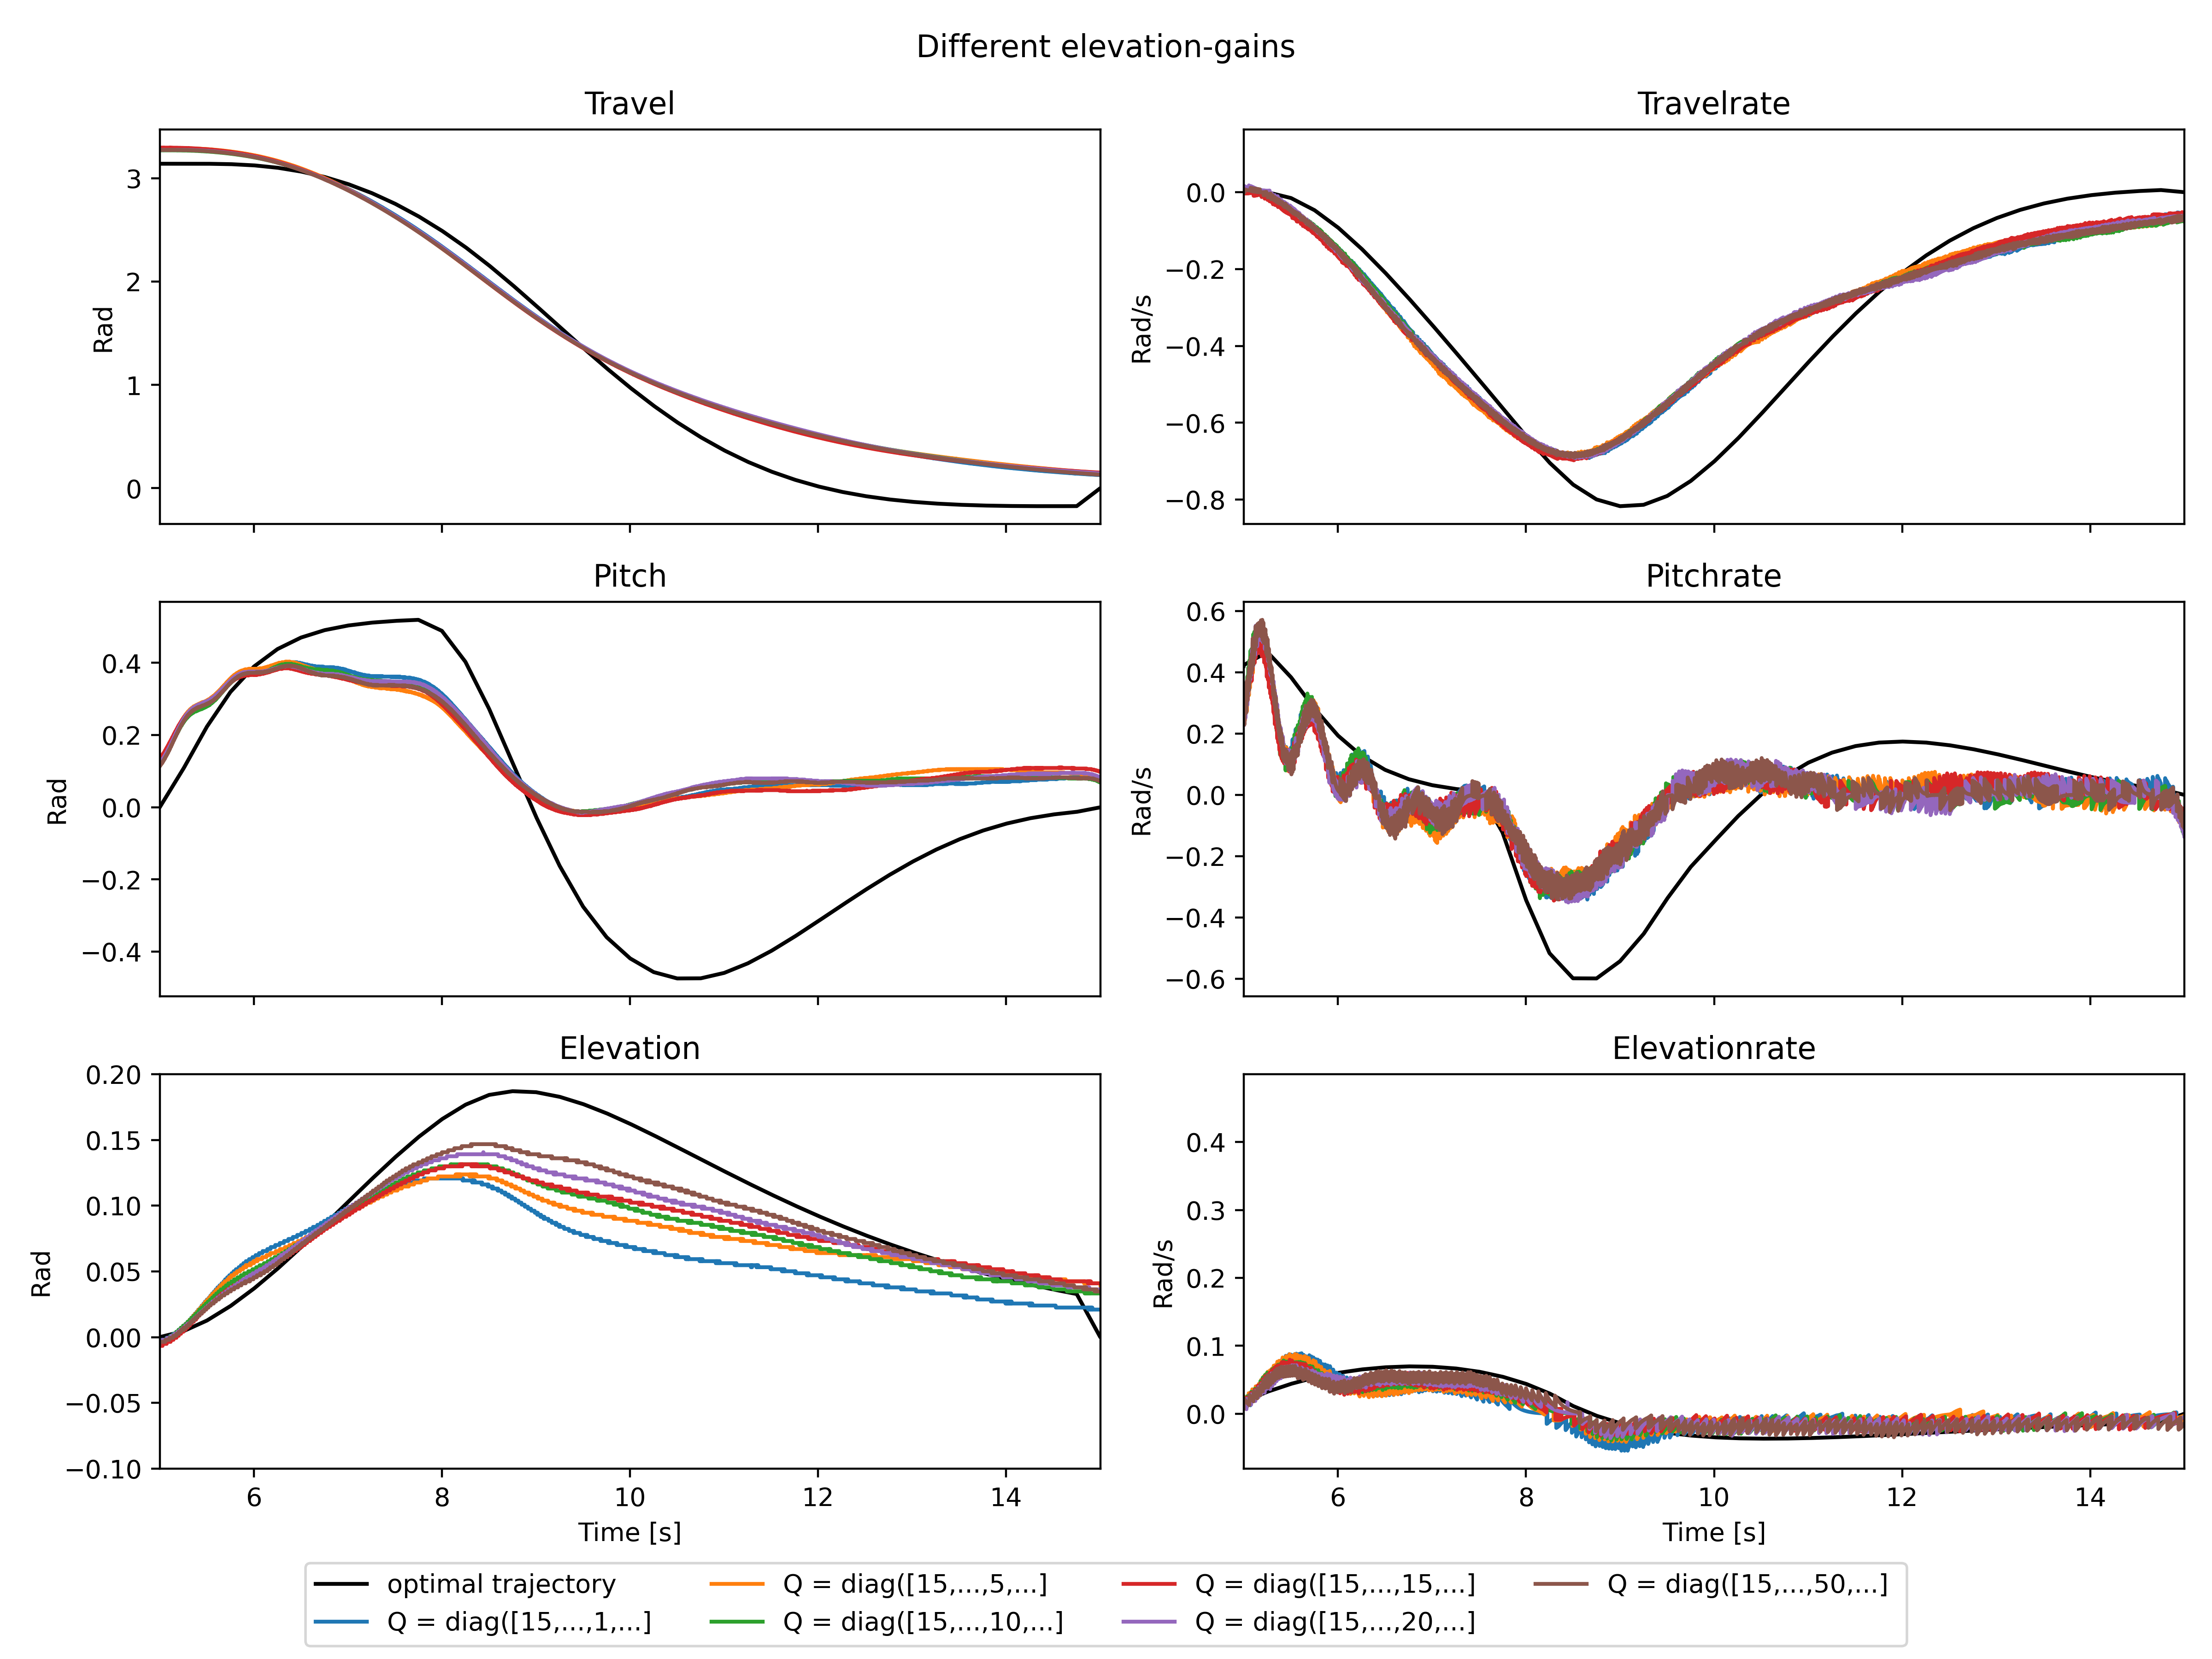
\includegraphics[width=\linewidth]{figures/LAB4_elevation_gains.png}
	\caption{Her er alle verdiene vi brukte, bør nok rydde opp litt.}
	\label{fig:lab4_diff_elevation_values}
\end{figure}

Using the same approach as in \todo{cref lab 3 }the group tuned entry-by-entry in $ \bm Q $. In the end the best tuning was achieved using: 
\begin{equation}\label{key}
	\bm Q = \begin{bmatrix}
		0 & 0 & 0 & 0 & 0 \\
		0 & 0 & 0 & 0 & 0 \\
		0 & 0 & 0 & 0 & 0 \\
		0 & 0 & 0 & 0 & 0 \\
		0 & 0 & 0 & 0 & 0 \\
	\end{bmatrix}, 
	\bm R = \begin{bmatrix}
		1 & 0 \\ 
		0 & 1
	\end{bmatrix}
\end{equation}

This gave the results in \cref{fig:LAB4_best_tuning}
\begin{figure}[h]
	\centering
	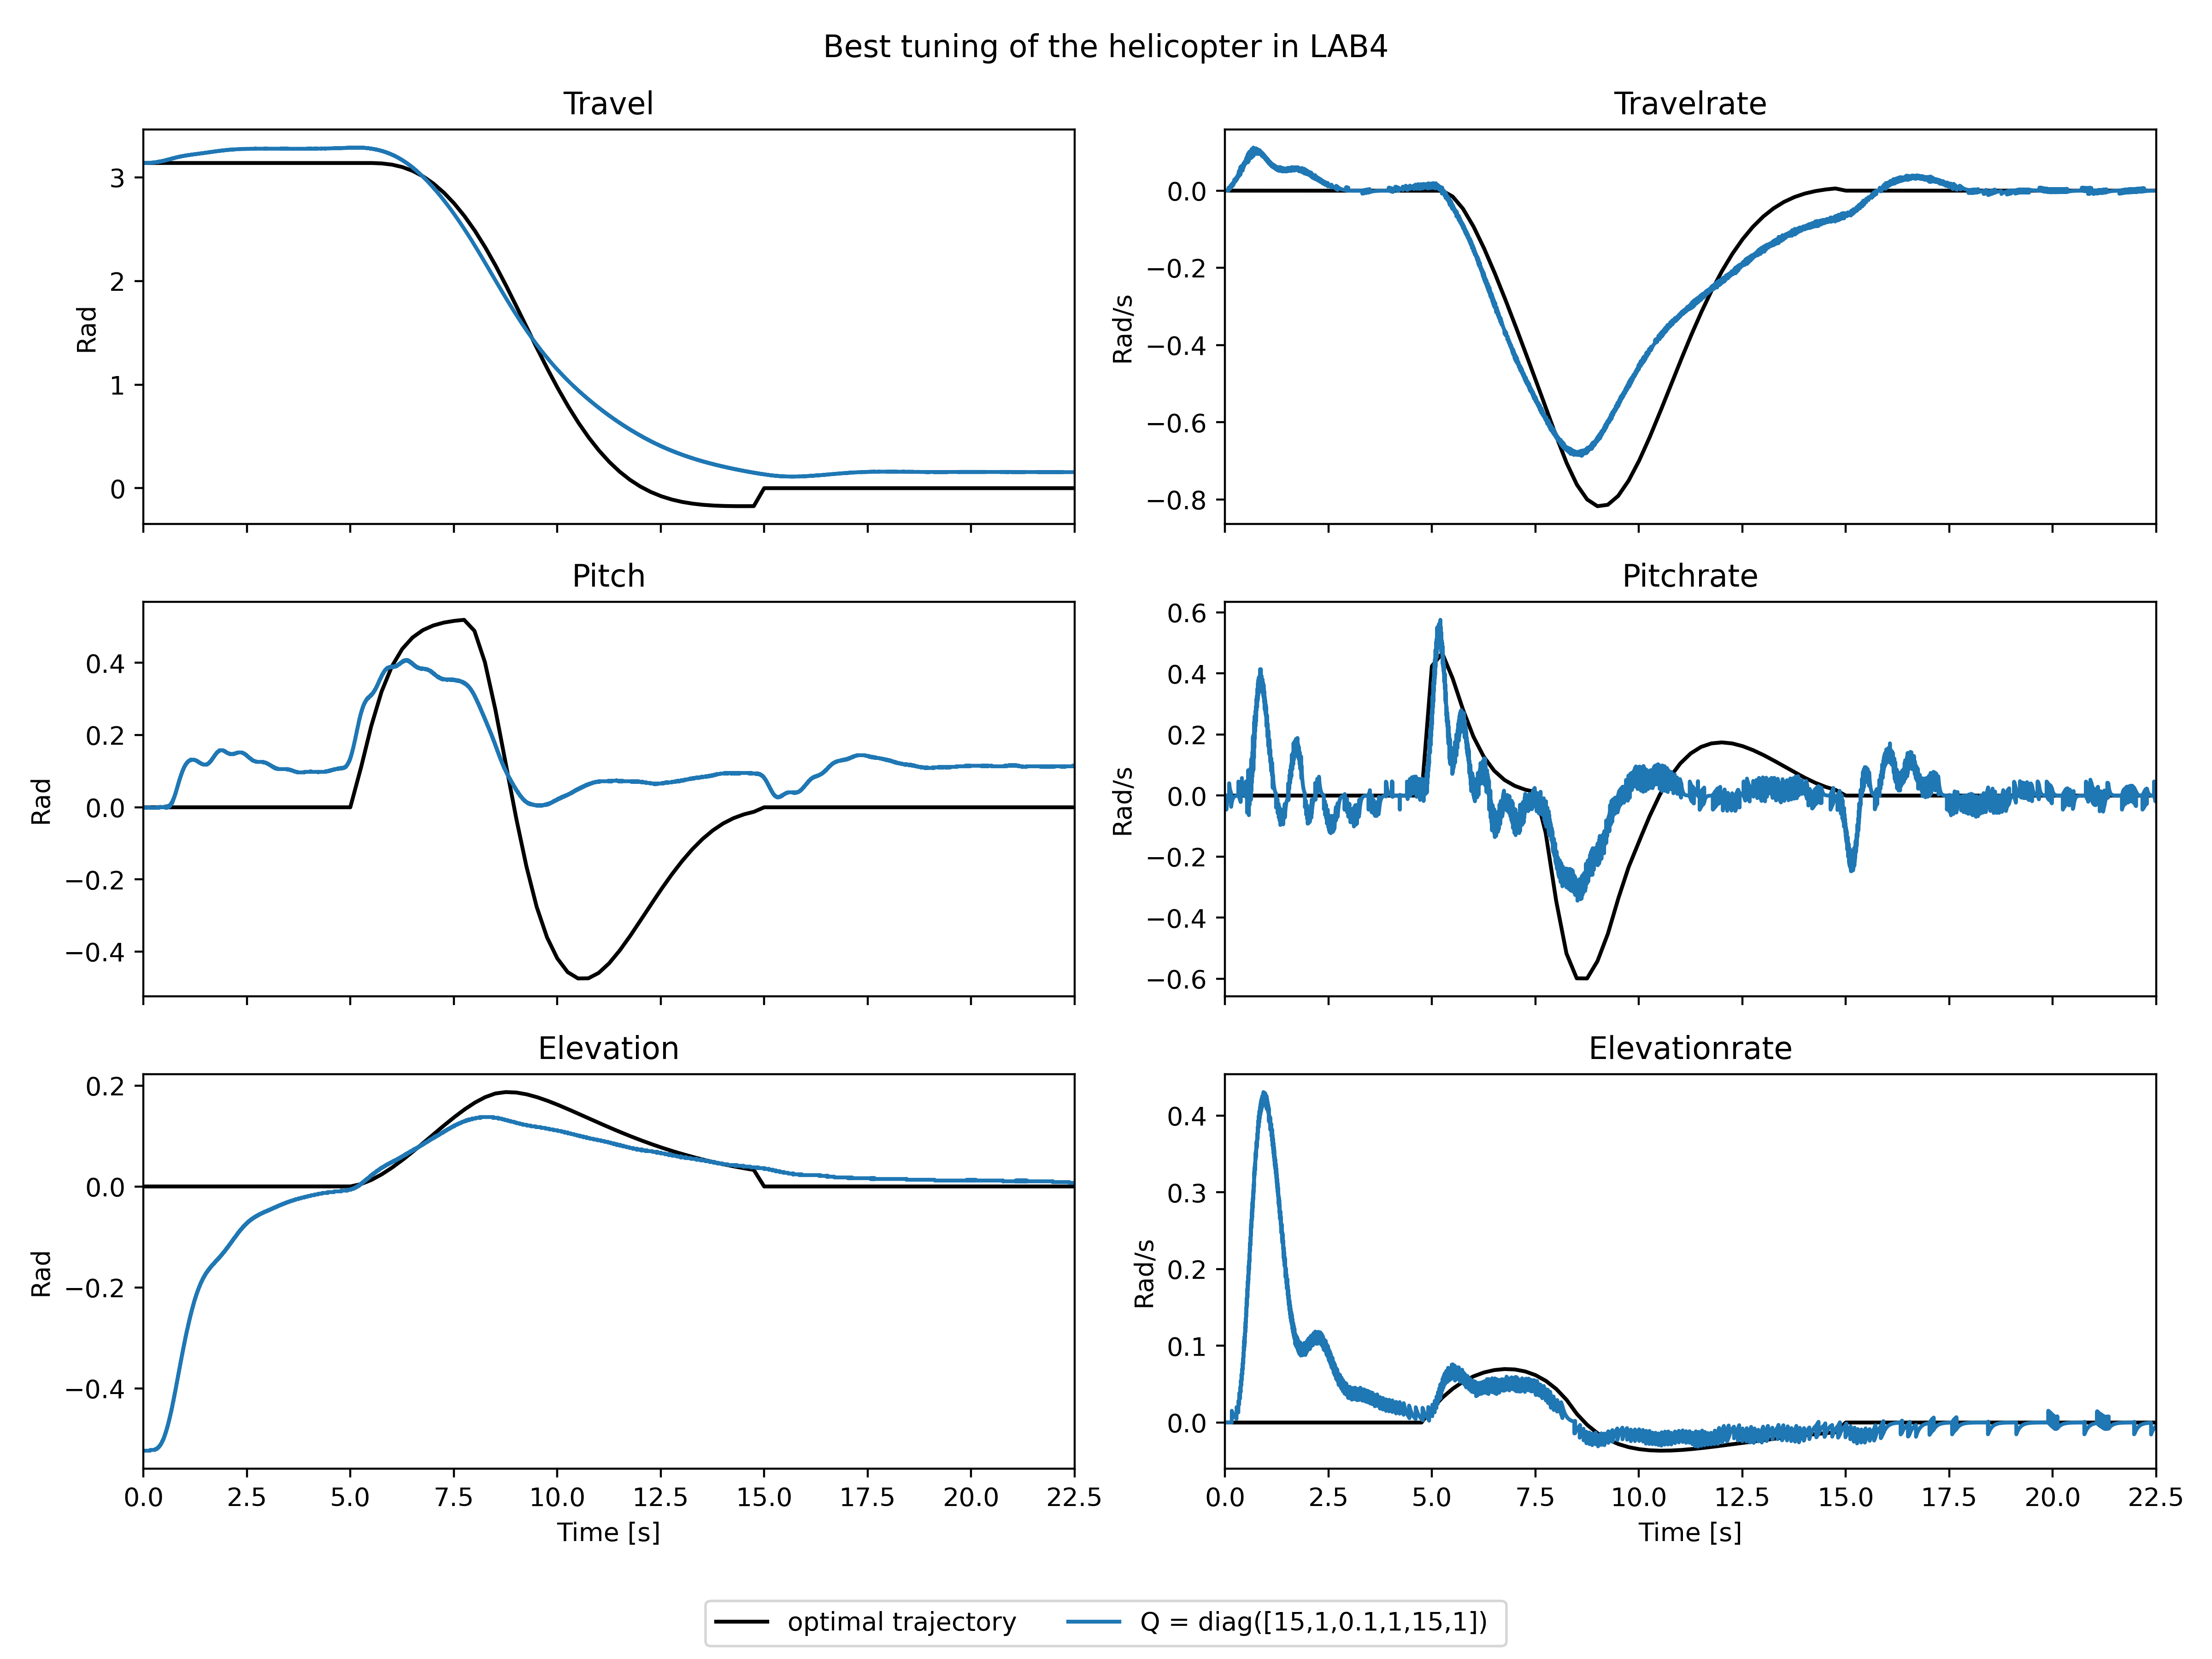
\includegraphics[width=\linewidth]{figures/LAB4_best_tunings.png}
	\caption{Best tuning}
	\label{fig:LAB4_best_tuning}
\end{figure}

\subsubsection{Finding a reasonable trajectory}
With a good
 

\subsection{Decoupled model} \label{sec:lab4_decoupled}
\textit{Answer 10.4.2.7}
As states in the problem description, the two last states are completely decoupled from the first four states. Or put in other words, the dynamics describing elevation is completely independent on the pitch and travel. This is of course not the case in reality, and illustrates how ``simple'' are model of the system actually is!

It becomes quite obvious from the plots \todo{Fin plots that shows this} that the elevation response is heavily coupled with both pitch and travel. Plot \todo{add cref} shows this as when the pitch is changed at time \todo{add time point}, the elevation also changes when it in fact should have been still as calculated in the optimal trajectory. Also there is a lot of rotational forces that have not been considered in the model. E.g. the travel rate $ r $ will create a centripetal force going along the helicopter arm, and point inwards to the origin of the arm. If the helicopter arm is not completely horizontal, this centripetal force will have a component in the direction of the elevation. The main point is that our model is a very simplified version of the real physics of the helicopter. In reality the helicopter is a complex system, which we can never define 100 \% exact with a mathematical formulation. It is impossible.

The effect this has on our optimal trajectory, is that our solver considers elevation as a system that is completely independent on the other states. The implication of this is that our optimal trajectory for elevation is the same, no matter how the trajectory for pitch and travel looks like. \todo[inline]{Is this statement correct? Test this} This can of course be turned the other way around, as the optimal pitch- and travel-trajectory is also independent on the optimal elevation trajectory. The optimal trajectories are ``wrong'', since the elevation is clearly not independent on the other states! Our helicopter will therefor have a hard time following the optimal trajectories as they are not a good representation of the reality.

\subsubsection{Possible solutions}
There are no correct solution to this problem, as we will never be able to describe the real-world system exact with mathematical formulations. There are however, some ``solutions'' that will improve our system and reduce the errors that arises from our decoupled model.

The obvious solution is to couple the model by making it more realistic. There are forces that we can include in our model to make it more accurate. These are for instance the centripetal force mentioned above, friction forces, forces caused by the ground effect, and so on. Of course we can only add simplified equations for these forces, but it would nevertheless increase the accuracy of our model! We will never be able to take into account all forces, and many forces are actually impossible to model mathematically. Therefore we need to identify the forces that has the biggest impact on the error in our model. This is a hard task in itself and can be considered a downside of this approach. Another downside is that our model will quickly become complex and hard to understand. However, the group thinks that it would not be to much work to take into account the most obvious rotational forces, which could possibly cause a big improvement in the optimal solution.

Another solution is not to change the mathematical model of the helicopter at all, but rather change the regulator for the helicopter. Maybe adding integral-effect in the pitch- and elevation-controller would help decreasing the error? Or maybe other feedback-loop implementations could yield better results? There are many possible solutions to improve the regulation of the helicopter! Using this ``solution'', our optimal solution will still be wrong, but we can reduce the error by using a better regulator. The advantage of this is that we can spend less time making a more exact mathematical model, and rather focus on making a regulator that is more robust for errors. The disadvantage is of course that our optimal trajectories are still wrong.



\subsection{MATLAB and Simulink}
\textit{Code and diagrams go here}

\subsection{Optional exercise}
\textit{Which constraints did you add? What was the results? Plots? Discussion?}
\end{document}

\begin{figure}
    \begin{center}
        %% Creator: Matplotlib, PGF backend
%%
%% To include the figure in your LaTeX document, write
%%   \input{<filename>.pgf}
%%
%% Make sure the required packages are loaded in your preamble
%%   \usepackage{pgf}
%%
%% and, on pdftex
%%   \usepackage[utf8]{inputenc}\DeclareUnicodeCharacter{2212}{-}
%%
%% or, on luatex and xetex
%%   \usepackage{unicode-math}
%%
%% Figures using additional raster images can only be included by \input if
%% they are in the same directory as the main LaTeX file. For loading figures
%% from other directories you can use the `import` package
%%   \usepackage{import}
%%
%% and then include the figures with
%%   \import{<path to file>}{<filename>.pgf}
%%
%% Matplotlib used the following preamble
%%
\begingroup%
\makeatletter%
\begin{pgfpicture}%
\pgfpathrectangle{\pgfpointorigin}{\pgfqpoint{6.400000in}{4.800000in}}%
\pgfusepath{use as bounding box, clip}%
\begin{pgfscope}%
\pgfsetbuttcap%
\pgfsetmiterjoin%
\definecolor{currentfill}{rgb}{1.000000,1.000000,1.000000}%
\pgfsetfillcolor{currentfill}%
\pgfsetlinewidth{0.000000pt}%
\definecolor{currentstroke}{rgb}{1.000000,1.000000,1.000000}%
\pgfsetstrokecolor{currentstroke}%
\pgfsetdash{}{0pt}%
\pgfpathmoveto{\pgfqpoint{0.000000in}{0.000000in}}%
\pgfpathlineto{\pgfqpoint{6.400000in}{0.000000in}}%
\pgfpathlineto{\pgfqpoint{6.400000in}{4.800000in}}%
\pgfpathlineto{\pgfqpoint{0.000000in}{4.800000in}}%
\pgfpathclose%
\pgfusepath{fill}%
\end{pgfscope}%
\begin{pgfscope}%
\pgfsetbuttcap%
\pgfsetmiterjoin%
\definecolor{currentfill}{rgb}{1.000000,1.000000,1.000000}%
\pgfsetfillcolor{currentfill}%
\pgfsetlinewidth{0.000000pt}%
\definecolor{currentstroke}{rgb}{0.000000,0.000000,0.000000}%
\pgfsetstrokecolor{currentstroke}%
\pgfsetstrokeopacity{0.000000}%
\pgfsetdash{}{0pt}%
\pgfpathmoveto{\pgfqpoint{0.800000in}{0.528000in}}%
\pgfpathlineto{\pgfqpoint{5.760000in}{0.528000in}}%
\pgfpathlineto{\pgfqpoint{5.760000in}{4.224000in}}%
\pgfpathlineto{\pgfqpoint{0.800000in}{4.224000in}}%
\pgfpathclose%
\pgfusepath{fill}%
\end{pgfscope}%
\begin{pgfscope}%
\pgfsetbuttcap%
\pgfsetroundjoin%
\definecolor{currentfill}{rgb}{0.000000,0.000000,0.000000}%
\pgfsetfillcolor{currentfill}%
\pgfsetlinewidth{0.803000pt}%
\definecolor{currentstroke}{rgb}{0.000000,0.000000,0.000000}%
\pgfsetstrokecolor{currentstroke}%
\pgfsetdash{}{0pt}%
\pgfsys@defobject{currentmarker}{\pgfqpoint{0.000000in}{-0.048611in}}{\pgfqpoint{0.000000in}{0.000000in}}{%
\pgfpathmoveto{\pgfqpoint{0.000000in}{0.000000in}}%
\pgfpathlineto{\pgfqpoint{0.000000in}{-0.048611in}}%
\pgfusepath{stroke,fill}%
}%
\begin{pgfscope}%
\pgfsys@transformshift{1.025455in}{0.528000in}%
\pgfsys@useobject{currentmarker}{}%
\end{pgfscope}%
\end{pgfscope}%
\begin{pgfscope}%
\definecolor{textcolor}{rgb}{0.000000,0.000000,0.000000}%
\pgfsetstrokecolor{textcolor}%
\pgfsetfillcolor{textcolor}%
\pgftext[x=1.025455in,y=0.430778in,,top]{\color{textcolor}\rmfamily\fontsize{10.000000}{12.000000}\selectfont \(\displaystyle {0}\)}%
\end{pgfscope}%
\begin{pgfscope}%
\pgfsetbuttcap%
\pgfsetroundjoin%
\definecolor{currentfill}{rgb}{0.000000,0.000000,0.000000}%
\pgfsetfillcolor{currentfill}%
\pgfsetlinewidth{0.803000pt}%
\definecolor{currentstroke}{rgb}{0.000000,0.000000,0.000000}%
\pgfsetstrokecolor{currentstroke}%
\pgfsetdash{}{0pt}%
\pgfsys@defobject{currentmarker}{\pgfqpoint{0.000000in}{-0.048611in}}{\pgfqpoint{0.000000in}{0.000000in}}{%
\pgfpathmoveto{\pgfqpoint{0.000000in}{0.000000in}}%
\pgfpathlineto{\pgfqpoint{0.000000in}{-0.048611in}}%
\pgfusepath{stroke,fill}%
}%
\begin{pgfscope}%
\pgfsys@transformshift{1.589091in}{0.528000in}%
\pgfsys@useobject{currentmarker}{}%
\end{pgfscope}%
\end{pgfscope}%
\begin{pgfscope}%
\definecolor{textcolor}{rgb}{0.000000,0.000000,0.000000}%
\pgfsetstrokecolor{textcolor}%
\pgfsetfillcolor{textcolor}%
\pgftext[x=1.589091in,y=0.430778in,,top]{\color{textcolor}\rmfamily\fontsize{10.000000}{12.000000}\selectfont \(\displaystyle {5}\)}%
\end{pgfscope}%
\begin{pgfscope}%
\pgfsetbuttcap%
\pgfsetroundjoin%
\definecolor{currentfill}{rgb}{0.000000,0.000000,0.000000}%
\pgfsetfillcolor{currentfill}%
\pgfsetlinewidth{0.803000pt}%
\definecolor{currentstroke}{rgb}{0.000000,0.000000,0.000000}%
\pgfsetstrokecolor{currentstroke}%
\pgfsetdash{}{0pt}%
\pgfsys@defobject{currentmarker}{\pgfqpoint{0.000000in}{-0.048611in}}{\pgfqpoint{0.000000in}{0.000000in}}{%
\pgfpathmoveto{\pgfqpoint{0.000000in}{0.000000in}}%
\pgfpathlineto{\pgfqpoint{0.000000in}{-0.048611in}}%
\pgfusepath{stroke,fill}%
}%
\begin{pgfscope}%
\pgfsys@transformshift{2.152727in}{0.528000in}%
\pgfsys@useobject{currentmarker}{}%
\end{pgfscope}%
\end{pgfscope}%
\begin{pgfscope}%
\definecolor{textcolor}{rgb}{0.000000,0.000000,0.000000}%
\pgfsetstrokecolor{textcolor}%
\pgfsetfillcolor{textcolor}%
\pgftext[x=2.152727in,y=0.430778in,,top]{\color{textcolor}\rmfamily\fontsize{10.000000}{12.000000}\selectfont \(\displaystyle {10}\)}%
\end{pgfscope}%
\begin{pgfscope}%
\pgfsetbuttcap%
\pgfsetroundjoin%
\definecolor{currentfill}{rgb}{0.000000,0.000000,0.000000}%
\pgfsetfillcolor{currentfill}%
\pgfsetlinewidth{0.803000pt}%
\definecolor{currentstroke}{rgb}{0.000000,0.000000,0.000000}%
\pgfsetstrokecolor{currentstroke}%
\pgfsetdash{}{0pt}%
\pgfsys@defobject{currentmarker}{\pgfqpoint{0.000000in}{-0.048611in}}{\pgfqpoint{0.000000in}{0.000000in}}{%
\pgfpathmoveto{\pgfqpoint{0.000000in}{0.000000in}}%
\pgfpathlineto{\pgfqpoint{0.000000in}{-0.048611in}}%
\pgfusepath{stroke,fill}%
}%
\begin{pgfscope}%
\pgfsys@transformshift{2.716364in}{0.528000in}%
\pgfsys@useobject{currentmarker}{}%
\end{pgfscope}%
\end{pgfscope}%
\begin{pgfscope}%
\definecolor{textcolor}{rgb}{0.000000,0.000000,0.000000}%
\pgfsetstrokecolor{textcolor}%
\pgfsetfillcolor{textcolor}%
\pgftext[x=2.716364in,y=0.430778in,,top]{\color{textcolor}\rmfamily\fontsize{10.000000}{12.000000}\selectfont \(\displaystyle {15}\)}%
\end{pgfscope}%
\begin{pgfscope}%
\pgfsetbuttcap%
\pgfsetroundjoin%
\definecolor{currentfill}{rgb}{0.000000,0.000000,0.000000}%
\pgfsetfillcolor{currentfill}%
\pgfsetlinewidth{0.803000pt}%
\definecolor{currentstroke}{rgb}{0.000000,0.000000,0.000000}%
\pgfsetstrokecolor{currentstroke}%
\pgfsetdash{}{0pt}%
\pgfsys@defobject{currentmarker}{\pgfqpoint{0.000000in}{-0.048611in}}{\pgfqpoint{0.000000in}{0.000000in}}{%
\pgfpathmoveto{\pgfqpoint{0.000000in}{0.000000in}}%
\pgfpathlineto{\pgfqpoint{0.000000in}{-0.048611in}}%
\pgfusepath{stroke,fill}%
}%
\begin{pgfscope}%
\pgfsys@transformshift{3.280000in}{0.528000in}%
\pgfsys@useobject{currentmarker}{}%
\end{pgfscope}%
\end{pgfscope}%
\begin{pgfscope}%
\definecolor{textcolor}{rgb}{0.000000,0.000000,0.000000}%
\pgfsetstrokecolor{textcolor}%
\pgfsetfillcolor{textcolor}%
\pgftext[x=3.280000in,y=0.430778in,,top]{\color{textcolor}\rmfamily\fontsize{10.000000}{12.000000}\selectfont \(\displaystyle {20}\)}%
\end{pgfscope}%
\begin{pgfscope}%
\pgfsetbuttcap%
\pgfsetroundjoin%
\definecolor{currentfill}{rgb}{0.000000,0.000000,0.000000}%
\pgfsetfillcolor{currentfill}%
\pgfsetlinewidth{0.803000pt}%
\definecolor{currentstroke}{rgb}{0.000000,0.000000,0.000000}%
\pgfsetstrokecolor{currentstroke}%
\pgfsetdash{}{0pt}%
\pgfsys@defobject{currentmarker}{\pgfqpoint{0.000000in}{-0.048611in}}{\pgfqpoint{0.000000in}{0.000000in}}{%
\pgfpathmoveto{\pgfqpoint{0.000000in}{0.000000in}}%
\pgfpathlineto{\pgfqpoint{0.000000in}{-0.048611in}}%
\pgfusepath{stroke,fill}%
}%
\begin{pgfscope}%
\pgfsys@transformshift{3.843636in}{0.528000in}%
\pgfsys@useobject{currentmarker}{}%
\end{pgfscope}%
\end{pgfscope}%
\begin{pgfscope}%
\definecolor{textcolor}{rgb}{0.000000,0.000000,0.000000}%
\pgfsetstrokecolor{textcolor}%
\pgfsetfillcolor{textcolor}%
\pgftext[x=3.843636in,y=0.430778in,,top]{\color{textcolor}\rmfamily\fontsize{10.000000}{12.000000}\selectfont \(\displaystyle {25}\)}%
\end{pgfscope}%
\begin{pgfscope}%
\pgfsetbuttcap%
\pgfsetroundjoin%
\definecolor{currentfill}{rgb}{0.000000,0.000000,0.000000}%
\pgfsetfillcolor{currentfill}%
\pgfsetlinewidth{0.803000pt}%
\definecolor{currentstroke}{rgb}{0.000000,0.000000,0.000000}%
\pgfsetstrokecolor{currentstroke}%
\pgfsetdash{}{0pt}%
\pgfsys@defobject{currentmarker}{\pgfqpoint{0.000000in}{-0.048611in}}{\pgfqpoint{0.000000in}{0.000000in}}{%
\pgfpathmoveto{\pgfqpoint{0.000000in}{0.000000in}}%
\pgfpathlineto{\pgfqpoint{0.000000in}{-0.048611in}}%
\pgfusepath{stroke,fill}%
}%
\begin{pgfscope}%
\pgfsys@transformshift{4.407273in}{0.528000in}%
\pgfsys@useobject{currentmarker}{}%
\end{pgfscope}%
\end{pgfscope}%
\begin{pgfscope}%
\definecolor{textcolor}{rgb}{0.000000,0.000000,0.000000}%
\pgfsetstrokecolor{textcolor}%
\pgfsetfillcolor{textcolor}%
\pgftext[x=4.407273in,y=0.430778in,,top]{\color{textcolor}\rmfamily\fontsize{10.000000}{12.000000}\selectfont \(\displaystyle {30}\)}%
\end{pgfscope}%
\begin{pgfscope}%
\pgfsetbuttcap%
\pgfsetroundjoin%
\definecolor{currentfill}{rgb}{0.000000,0.000000,0.000000}%
\pgfsetfillcolor{currentfill}%
\pgfsetlinewidth{0.803000pt}%
\definecolor{currentstroke}{rgb}{0.000000,0.000000,0.000000}%
\pgfsetstrokecolor{currentstroke}%
\pgfsetdash{}{0pt}%
\pgfsys@defobject{currentmarker}{\pgfqpoint{0.000000in}{-0.048611in}}{\pgfqpoint{0.000000in}{0.000000in}}{%
\pgfpathmoveto{\pgfqpoint{0.000000in}{0.000000in}}%
\pgfpathlineto{\pgfqpoint{0.000000in}{-0.048611in}}%
\pgfusepath{stroke,fill}%
}%
\begin{pgfscope}%
\pgfsys@transformshift{4.970909in}{0.528000in}%
\pgfsys@useobject{currentmarker}{}%
\end{pgfscope}%
\end{pgfscope}%
\begin{pgfscope}%
\definecolor{textcolor}{rgb}{0.000000,0.000000,0.000000}%
\pgfsetstrokecolor{textcolor}%
\pgfsetfillcolor{textcolor}%
\pgftext[x=4.970909in,y=0.430778in,,top]{\color{textcolor}\rmfamily\fontsize{10.000000}{12.000000}\selectfont \(\displaystyle {35}\)}%
\end{pgfscope}%
\begin{pgfscope}%
\pgfsetbuttcap%
\pgfsetroundjoin%
\definecolor{currentfill}{rgb}{0.000000,0.000000,0.000000}%
\pgfsetfillcolor{currentfill}%
\pgfsetlinewidth{0.803000pt}%
\definecolor{currentstroke}{rgb}{0.000000,0.000000,0.000000}%
\pgfsetstrokecolor{currentstroke}%
\pgfsetdash{}{0pt}%
\pgfsys@defobject{currentmarker}{\pgfqpoint{0.000000in}{-0.048611in}}{\pgfqpoint{0.000000in}{0.000000in}}{%
\pgfpathmoveto{\pgfqpoint{0.000000in}{0.000000in}}%
\pgfpathlineto{\pgfqpoint{0.000000in}{-0.048611in}}%
\pgfusepath{stroke,fill}%
}%
\begin{pgfscope}%
\pgfsys@transformshift{5.534545in}{0.528000in}%
\pgfsys@useobject{currentmarker}{}%
\end{pgfscope}%
\end{pgfscope}%
\begin{pgfscope}%
\definecolor{textcolor}{rgb}{0.000000,0.000000,0.000000}%
\pgfsetstrokecolor{textcolor}%
\pgfsetfillcolor{textcolor}%
\pgftext[x=5.534545in,y=0.430778in,,top]{\color{textcolor}\rmfamily\fontsize{10.000000}{12.000000}\selectfont \(\displaystyle {40}\)}%
\end{pgfscope}%
\begin{pgfscope}%
\definecolor{textcolor}{rgb}{0.000000,0.000000,0.000000}%
\pgfsetstrokecolor{textcolor}%
\pgfsetfillcolor{textcolor}%
\pgftext[x=3.280000in,y=0.251766in,,top]{\color{textcolor}\rmfamily\fontsize{10.000000}{12.000000}\selectfont time [s]}%
\end{pgfscope}%
\begin{pgfscope}%
\pgfsetbuttcap%
\pgfsetroundjoin%
\definecolor{currentfill}{rgb}{0.000000,0.000000,0.000000}%
\pgfsetfillcolor{currentfill}%
\pgfsetlinewidth{0.803000pt}%
\definecolor{currentstroke}{rgb}{0.000000,0.000000,0.000000}%
\pgfsetstrokecolor{currentstroke}%
\pgfsetdash{}{0pt}%
\pgfsys@defobject{currentmarker}{\pgfqpoint{-0.048611in}{0.000000in}}{\pgfqpoint{-0.000000in}{0.000000in}}{%
\pgfpathmoveto{\pgfqpoint{-0.000000in}{0.000000in}}%
\pgfpathlineto{\pgfqpoint{-0.048611in}{0.000000in}}%
\pgfusepath{stroke,fill}%
}%
\begin{pgfscope}%
\pgfsys@transformshift{0.800000in}{0.798142in}%
\pgfsys@useobject{currentmarker}{}%
\end{pgfscope}%
\end{pgfscope}%
\begin{pgfscope}%
\definecolor{textcolor}{rgb}{0.000000,0.000000,0.000000}%
\pgfsetstrokecolor{textcolor}%
\pgfsetfillcolor{textcolor}%
\pgftext[x=0.633333in, y=0.749917in, left, base]{\color{textcolor}\rmfamily\fontsize{10.000000}{12.000000}\selectfont \(\displaystyle {0}\)}%
\end{pgfscope}%
\begin{pgfscope}%
\pgfsetbuttcap%
\pgfsetroundjoin%
\definecolor{currentfill}{rgb}{0.000000,0.000000,0.000000}%
\pgfsetfillcolor{currentfill}%
\pgfsetlinewidth{0.803000pt}%
\definecolor{currentstroke}{rgb}{0.000000,0.000000,0.000000}%
\pgfsetstrokecolor{currentstroke}%
\pgfsetdash{}{0pt}%
\pgfsys@defobject{currentmarker}{\pgfqpoint{-0.048611in}{0.000000in}}{\pgfqpoint{-0.000000in}{0.000000in}}{%
\pgfpathmoveto{\pgfqpoint{-0.000000in}{0.000000in}}%
\pgfpathlineto{\pgfqpoint{-0.048611in}{0.000000in}}%
\pgfusepath{stroke,fill}%
}%
\begin{pgfscope}%
\pgfsys@transformshift{0.800000in}{1.521850in}%
\pgfsys@useobject{currentmarker}{}%
\end{pgfscope}%
\end{pgfscope}%
\begin{pgfscope}%
\definecolor{textcolor}{rgb}{0.000000,0.000000,0.000000}%
\pgfsetstrokecolor{textcolor}%
\pgfsetfillcolor{textcolor}%
\pgftext[x=0.633333in, y=1.473625in, left, base]{\color{textcolor}\rmfamily\fontsize{10.000000}{12.000000}\selectfont \(\displaystyle {5}\)}%
\end{pgfscope}%
\begin{pgfscope}%
\pgfsetbuttcap%
\pgfsetroundjoin%
\definecolor{currentfill}{rgb}{0.000000,0.000000,0.000000}%
\pgfsetfillcolor{currentfill}%
\pgfsetlinewidth{0.803000pt}%
\definecolor{currentstroke}{rgb}{0.000000,0.000000,0.000000}%
\pgfsetstrokecolor{currentstroke}%
\pgfsetdash{}{0pt}%
\pgfsys@defobject{currentmarker}{\pgfqpoint{-0.048611in}{0.000000in}}{\pgfqpoint{-0.000000in}{0.000000in}}{%
\pgfpathmoveto{\pgfqpoint{-0.000000in}{0.000000in}}%
\pgfpathlineto{\pgfqpoint{-0.048611in}{0.000000in}}%
\pgfusepath{stroke,fill}%
}%
\begin{pgfscope}%
\pgfsys@transformshift{0.800000in}{2.245558in}%
\pgfsys@useobject{currentmarker}{}%
\end{pgfscope}%
\end{pgfscope}%
\begin{pgfscope}%
\definecolor{textcolor}{rgb}{0.000000,0.000000,0.000000}%
\pgfsetstrokecolor{textcolor}%
\pgfsetfillcolor{textcolor}%
\pgftext[x=0.563888in, y=2.197333in, left, base]{\color{textcolor}\rmfamily\fontsize{10.000000}{12.000000}\selectfont \(\displaystyle {10}\)}%
\end{pgfscope}%
\begin{pgfscope}%
\pgfsetbuttcap%
\pgfsetroundjoin%
\definecolor{currentfill}{rgb}{0.000000,0.000000,0.000000}%
\pgfsetfillcolor{currentfill}%
\pgfsetlinewidth{0.803000pt}%
\definecolor{currentstroke}{rgb}{0.000000,0.000000,0.000000}%
\pgfsetstrokecolor{currentstroke}%
\pgfsetdash{}{0pt}%
\pgfsys@defobject{currentmarker}{\pgfqpoint{-0.048611in}{0.000000in}}{\pgfqpoint{-0.000000in}{0.000000in}}{%
\pgfpathmoveto{\pgfqpoint{-0.000000in}{0.000000in}}%
\pgfpathlineto{\pgfqpoint{-0.048611in}{0.000000in}}%
\pgfusepath{stroke,fill}%
}%
\begin{pgfscope}%
\pgfsys@transformshift{0.800000in}{2.969266in}%
\pgfsys@useobject{currentmarker}{}%
\end{pgfscope}%
\end{pgfscope}%
\begin{pgfscope}%
\definecolor{textcolor}{rgb}{0.000000,0.000000,0.000000}%
\pgfsetstrokecolor{textcolor}%
\pgfsetfillcolor{textcolor}%
\pgftext[x=0.563888in, y=2.921041in, left, base]{\color{textcolor}\rmfamily\fontsize{10.000000}{12.000000}\selectfont \(\displaystyle {15}\)}%
\end{pgfscope}%
\begin{pgfscope}%
\pgfsetbuttcap%
\pgfsetroundjoin%
\definecolor{currentfill}{rgb}{0.000000,0.000000,0.000000}%
\pgfsetfillcolor{currentfill}%
\pgfsetlinewidth{0.803000pt}%
\definecolor{currentstroke}{rgb}{0.000000,0.000000,0.000000}%
\pgfsetstrokecolor{currentstroke}%
\pgfsetdash{}{0pt}%
\pgfsys@defobject{currentmarker}{\pgfqpoint{-0.048611in}{0.000000in}}{\pgfqpoint{-0.000000in}{0.000000in}}{%
\pgfpathmoveto{\pgfqpoint{-0.000000in}{0.000000in}}%
\pgfpathlineto{\pgfqpoint{-0.048611in}{0.000000in}}%
\pgfusepath{stroke,fill}%
}%
\begin{pgfscope}%
\pgfsys@transformshift{0.800000in}{3.692974in}%
\pgfsys@useobject{currentmarker}{}%
\end{pgfscope}%
\end{pgfscope}%
\begin{pgfscope}%
\definecolor{textcolor}{rgb}{0.000000,0.000000,0.000000}%
\pgfsetstrokecolor{textcolor}%
\pgfsetfillcolor{textcolor}%
\pgftext[x=0.563888in, y=3.644748in, left, base]{\color{textcolor}\rmfamily\fontsize{10.000000}{12.000000}\selectfont \(\displaystyle {20}\)}%
\end{pgfscope}%
\begin{pgfscope}%
\pgfpathrectangle{\pgfqpoint{0.800000in}{0.528000in}}{\pgfqpoint{4.960000in}{3.696000in}}%
\pgfusepath{clip}%
\pgfsetrectcap%
\pgfsetroundjoin%
\pgfsetlinewidth{1.505625pt}%
\definecolor{currentstroke}{rgb}{0.121569,0.466667,0.705882}%
\pgfsetstrokecolor{currentstroke}%
\pgfsetdash{}{0pt}%
\pgfpathmoveto{\pgfqpoint{1.025455in}{1.252861in}}%
\pgfpathlineto{\pgfqpoint{1.060851in}{1.253972in}}%
\pgfpathlineto{\pgfqpoint{1.064007in}{1.254305in}}%
\pgfpathlineto{\pgfqpoint{1.076182in}{1.255304in}}%
\pgfpathlineto{\pgfqpoint{1.077985in}{1.255637in}}%
\pgfpathlineto{\pgfqpoint{1.091287in}{1.256747in}}%
\pgfpathlineto{\pgfqpoint{1.094669in}{1.257191in}}%
\pgfpathlineto{\pgfqpoint{1.106393in}{1.258301in}}%
\pgfpathlineto{\pgfqpoint{1.109549in}{1.258634in}}%
\pgfpathlineto{\pgfqpoint{1.121724in}{1.259744in}}%
\pgfpathlineto{\pgfqpoint{1.124880in}{1.260077in}}%
\pgfpathlineto{\pgfqpoint{1.138182in}{1.261188in}}%
\pgfpathlineto{\pgfqpoint{1.141338in}{1.261521in}}%
\pgfpathlineto{\pgfqpoint{1.155091in}{1.262631in}}%
\pgfpathlineto{\pgfqpoint{1.158247in}{1.262964in}}%
\pgfpathlineto{\pgfqpoint{1.172000in}{1.264074in}}%
\pgfpathlineto{\pgfqpoint{1.175156in}{1.264407in}}%
\pgfpathlineto{\pgfqpoint{1.188233in}{1.265517in}}%
\pgfpathlineto{\pgfqpoint{1.191389in}{1.265850in}}%
\pgfpathlineto{\pgfqpoint{1.203338in}{1.266960in}}%
\pgfpathlineto{\pgfqpoint{1.206495in}{1.267293in}}%
\pgfpathlineto{\pgfqpoint{1.217542in}{1.268404in}}%
\pgfpathlineto{\pgfqpoint{1.220924in}{1.268848in}}%
\pgfpathlineto{\pgfqpoint{1.231520in}{1.269958in}}%
\pgfpathlineto{\pgfqpoint{1.234902in}{1.270402in}}%
\pgfpathlineto{\pgfqpoint{1.244822in}{1.271512in}}%
\pgfpathlineto{\pgfqpoint{1.248204in}{1.271956in}}%
\pgfpathlineto{\pgfqpoint{1.257222in}{1.273066in}}%
\pgfpathlineto{\pgfqpoint{1.260829in}{1.273621in}}%
\pgfpathlineto{\pgfqpoint{1.269847in}{1.274732in}}%
\pgfpathlineto{\pgfqpoint{1.273455in}{1.275287in}}%
\pgfpathlineto{\pgfqpoint{1.282247in}{1.276397in}}%
\pgfpathlineto{\pgfqpoint{1.285855in}{1.276952in}}%
\pgfpathlineto{\pgfqpoint{1.293971in}{1.278062in}}%
\pgfpathlineto{\pgfqpoint{1.297578in}{1.278617in}}%
\pgfpathlineto{\pgfqpoint{1.305469in}{1.279727in}}%
\pgfpathlineto{\pgfqpoint{1.309302in}{1.280393in}}%
\pgfpathlineto{\pgfqpoint{1.317644in}{1.281503in}}%
\pgfpathlineto{\pgfqpoint{1.321476in}{1.282170in}}%
\pgfpathlineto{\pgfqpoint{1.329142in}{1.283280in}}%
\pgfpathlineto{\pgfqpoint{1.332975in}{1.283946in}}%
\pgfpathlineto{\pgfqpoint{1.340415in}{1.285056in}}%
\pgfpathlineto{\pgfqpoint{1.344247in}{1.285722in}}%
\pgfpathlineto{\pgfqpoint{1.351011in}{1.286832in}}%
\pgfpathlineto{\pgfqpoint{1.354844in}{1.287498in}}%
\pgfpathlineto{\pgfqpoint{1.361833in}{1.288608in}}%
\pgfpathlineto{\pgfqpoint{1.365665in}{1.289275in}}%
\pgfpathlineto{\pgfqpoint{1.372204in}{1.290385in}}%
\pgfpathlineto{\pgfqpoint{1.376262in}{1.291162in}}%
\pgfpathlineto{\pgfqpoint{1.383025in}{1.292272in}}%
\pgfpathlineto{\pgfqpoint{1.387084in}{1.293049in}}%
\pgfpathlineto{\pgfqpoint{1.393622in}{1.294159in}}%
\pgfpathlineto{\pgfqpoint{1.397680in}{1.294936in}}%
\pgfpathlineto{\pgfqpoint{1.403993in}{1.296046in}}%
\pgfpathlineto{\pgfqpoint{1.408051in}{1.296824in}}%
\pgfpathlineto{\pgfqpoint{1.414138in}{1.297934in}}%
\pgfpathlineto{\pgfqpoint{1.418422in}{1.298822in}}%
\pgfpathlineto{\pgfqpoint{1.424735in}{1.299932in}}%
\pgfpathlineto{\pgfqpoint{1.429018in}{1.300820in}}%
\pgfpathlineto{\pgfqpoint{1.435105in}{1.301930in}}%
\pgfpathlineto{\pgfqpoint{1.439389in}{1.302818in}}%
\pgfpathlineto{\pgfqpoint{1.445251in}{1.303929in}}%
\pgfpathlineto{\pgfqpoint{1.449760in}{1.304928in}}%
\pgfpathlineto{\pgfqpoint{1.455622in}{1.306038in}}%
\pgfpathlineto{\pgfqpoint{1.460131in}{1.307037in}}%
\pgfpathlineto{\pgfqpoint{1.465993in}{1.308147in}}%
\pgfpathlineto{\pgfqpoint{1.470502in}{1.309146in}}%
\pgfpathlineto{\pgfqpoint{1.476138in}{1.310256in}}%
\pgfpathlineto{\pgfqpoint{1.480647in}{1.311256in}}%
\pgfpathlineto{\pgfqpoint{1.486284in}{1.312366in}}%
\pgfpathlineto{\pgfqpoint{1.490793in}{1.313365in}}%
\pgfpathlineto{\pgfqpoint{1.496204in}{1.314475in}}%
\pgfpathlineto{\pgfqpoint{1.500713in}{1.315474in}}%
\pgfpathlineto{\pgfqpoint{1.505898in}{1.316584in}}%
\pgfpathlineto{\pgfqpoint{1.510633in}{1.317694in}}%
\pgfpathlineto{\pgfqpoint{1.516044in}{1.318805in}}%
\pgfpathlineto{\pgfqpoint{1.520778in}{1.319915in}}%
\pgfpathlineto{\pgfqpoint{1.525964in}{1.321025in}}%
\pgfpathlineto{\pgfqpoint{1.530698in}{1.322135in}}%
\pgfpathlineto{\pgfqpoint{1.535658in}{1.323245in}}%
\pgfpathlineto{\pgfqpoint{1.540618in}{1.324466in}}%
\pgfpathlineto{\pgfqpoint{1.545578in}{1.325577in}}%
\pgfpathlineto{\pgfqpoint{1.550313in}{1.326687in}}%
\pgfpathlineto{\pgfqpoint{1.555273in}{1.327797in}}%
\pgfpathlineto{\pgfqpoint{1.560458in}{1.329129in}}%
\pgfpathlineto{\pgfqpoint{1.565193in}{1.330239in}}%
\pgfpathlineto{\pgfqpoint{1.570153in}{1.331460in}}%
\pgfpathlineto{\pgfqpoint{1.574887in}{1.332571in}}%
\pgfpathlineto{\pgfqpoint{1.580073in}{1.333903in}}%
\pgfpathlineto{\pgfqpoint{1.584807in}{1.335013in}}%
\pgfpathlineto{\pgfqpoint{1.590218in}{1.336456in}}%
\pgfpathlineto{\pgfqpoint{1.594953in}{1.337566in}}%
\pgfpathlineto{\pgfqpoint{1.600364in}{1.339009in}}%
\pgfpathlineto{\pgfqpoint{1.605324in}{1.340120in}}%
\pgfpathlineto{\pgfqpoint{1.610509in}{1.341452in}}%
\pgfpathlineto{\pgfqpoint{1.615695in}{1.342562in}}%
\pgfpathlineto{\pgfqpoint{1.620880in}{1.343894in}}%
\pgfpathlineto{\pgfqpoint{1.625840in}{1.345004in}}%
\pgfpathlineto{\pgfqpoint{1.630349in}{1.346003in}}%
\pgfpathlineto{\pgfqpoint{1.635760in}{1.347114in}}%
\pgfpathlineto{\pgfqpoint{1.640269in}{1.348113in}}%
\pgfpathlineto{\pgfqpoint{1.646356in}{1.349223in}}%
\pgfpathlineto{\pgfqpoint{1.650640in}{1.350111in}}%
\pgfpathlineto{\pgfqpoint{1.657629in}{1.351221in}}%
\pgfpathlineto{\pgfqpoint{1.661236in}{1.351776in}}%
\pgfpathlineto{\pgfqpoint{1.669127in}{1.352886in}}%
\pgfpathlineto{\pgfqpoint{1.672735in}{1.353441in}}%
\pgfpathlineto{\pgfqpoint{1.683331in}{1.354552in}}%
\pgfpathlineto{\pgfqpoint{1.686713in}{1.354996in}}%
\pgfpathlineto{\pgfqpoint{1.704975in}{1.356106in}}%
\pgfpathlineto{\pgfqpoint{1.707680in}{1.356217in}}%
\pgfpathlineto{\pgfqpoint{1.745331in}{1.355107in}}%
\pgfpathlineto{\pgfqpoint{1.748487in}{1.354774in}}%
\pgfpathlineto{\pgfqpoint{1.757731in}{1.353663in}}%
\pgfpathlineto{\pgfqpoint{1.761113in}{1.353219in}}%
\pgfpathlineto{\pgfqpoint{1.768102in}{1.352109in}}%
\pgfpathlineto{\pgfqpoint{1.772385in}{1.351221in}}%
\pgfpathlineto{\pgfqpoint{1.778022in}{1.350111in}}%
\pgfpathlineto{\pgfqpoint{1.782756in}{1.349001in}}%
\pgfpathlineto{\pgfqpoint{1.787491in}{1.347891in}}%
\pgfpathlineto{\pgfqpoint{1.792676in}{1.346558in}}%
\pgfpathlineto{\pgfqpoint{1.796735in}{1.345448in}}%
\pgfpathlineto{\pgfqpoint{1.803047in}{1.343561in}}%
\pgfpathlineto{\pgfqpoint{1.806429in}{1.342451in}}%
\pgfpathlineto{\pgfqpoint{1.814996in}{1.339453in}}%
\pgfpathlineto{\pgfqpoint{1.818378in}{1.338343in}}%
\pgfpathlineto{\pgfqpoint{1.831680in}{1.333015in}}%
\pgfpathlineto{\pgfqpoint{1.834385in}{1.331904in}}%
\pgfpathlineto{\pgfqpoint{1.877447in}{1.309479in}}%
\pgfpathlineto{\pgfqpoint{1.881956in}{1.306593in}}%
\pgfpathlineto{\pgfqpoint{1.890749in}{1.301042in}}%
\pgfpathlineto{\pgfqpoint{1.895935in}{1.297490in}}%
\pgfpathlineto{\pgfqpoint{1.902473in}{1.293049in}}%
\pgfpathlineto{\pgfqpoint{1.908335in}{1.288830in}}%
\pgfpathlineto{\pgfqpoint{1.913295in}{1.285167in}}%
\pgfpathlineto{\pgfqpoint{1.920284in}{1.279838in}}%
\pgfpathlineto{\pgfqpoint{1.925018in}{1.276286in}}%
\pgfpathlineto{\pgfqpoint{1.933811in}{1.269181in}}%
\pgfpathlineto{\pgfqpoint{1.937644in}{1.266072in}}%
\pgfpathlineto{\pgfqpoint{1.947564in}{1.257857in}}%
\pgfpathlineto{\pgfqpoint{1.950945in}{1.254971in}}%
\pgfpathlineto{\pgfqpoint{1.964022in}{1.243647in}}%
\pgfpathlineto{\pgfqpoint{1.967404in}{1.240761in}}%
\pgfpathlineto{\pgfqpoint{1.984538in}{1.225441in}}%
\pgfpathlineto{\pgfqpoint{1.987695in}{1.222665in}}%
\pgfpathlineto{\pgfqpoint{2.006858in}{1.205347in}}%
\pgfpathlineto{\pgfqpoint{2.010015in}{1.202572in}}%
\pgfpathlineto{\pgfqpoint{2.026924in}{1.187473in}}%
\pgfpathlineto{\pgfqpoint{2.030080in}{1.184698in}}%
\pgfpathlineto{\pgfqpoint{2.043382in}{1.173152in}}%
\pgfpathlineto{\pgfqpoint{2.046989in}{1.170155in}}%
\pgfpathlineto{\pgfqpoint{2.057811in}{1.161052in}}%
\pgfpathlineto{\pgfqpoint{2.061644in}{1.157943in}}%
\pgfpathlineto{\pgfqpoint{2.070436in}{1.150838in}}%
\pgfpathlineto{\pgfqpoint{2.074720in}{1.147508in}}%
\pgfpathlineto{\pgfqpoint{2.081935in}{1.141957in}}%
\pgfpathlineto{\pgfqpoint{2.086669in}{1.138405in}}%
\pgfpathlineto{\pgfqpoint{2.092982in}{1.133742in}}%
\pgfpathlineto{\pgfqpoint{2.098393in}{1.129856in}}%
\pgfpathlineto{\pgfqpoint{2.104029in}{1.125860in}}%
\pgfpathlineto{\pgfqpoint{2.111920in}{1.120753in}}%
\pgfpathlineto{\pgfqpoint{2.116655in}{1.117645in}}%
\pgfpathlineto{\pgfqpoint{2.126800in}{1.111428in}}%
\pgfpathlineto{\pgfqpoint{2.130633in}{1.109208in}}%
\pgfpathlineto{\pgfqpoint{2.180458in}{1.085894in}}%
\pgfpathlineto{\pgfqpoint{2.184065in}{1.084784in}}%
\pgfpathlineto{\pgfqpoint{2.191505in}{1.082342in}}%
\pgfpathlineto{\pgfqpoint{2.196015in}{1.081232in}}%
\pgfpathlineto{\pgfqpoint{2.201200in}{1.079900in}}%
\pgfpathlineto{\pgfqpoint{2.206160in}{1.078789in}}%
\pgfpathlineto{\pgfqpoint{2.210669in}{1.077790in}}%
\pgfpathlineto{\pgfqpoint{2.217433in}{1.076680in}}%
\pgfpathlineto{\pgfqpoint{2.220815in}{1.076125in}}%
\pgfpathlineto{\pgfqpoint{2.222844in}{1.075903in}}%
\pgfpathlineto{\pgfqpoint{2.236371in}{1.074793in}}%
\pgfpathlineto{\pgfqpoint{2.239302in}{1.074571in}}%
\pgfpathlineto{\pgfqpoint{2.267484in}{1.075681in}}%
\pgfpathlineto{\pgfqpoint{2.270865in}{1.076125in}}%
\pgfpathlineto{\pgfqpoint{2.279207in}{1.077235in}}%
\pgfpathlineto{\pgfqpoint{2.283716in}{1.078234in}}%
\pgfpathlineto{\pgfqpoint{2.289804in}{1.079344in}}%
\pgfpathlineto{\pgfqpoint{2.294989in}{1.080677in}}%
\pgfpathlineto{\pgfqpoint{2.299949in}{1.081787in}}%
\pgfpathlineto{\pgfqpoint{2.306262in}{1.083674in}}%
\pgfpathlineto{\pgfqpoint{2.309869in}{1.084784in}}%
\pgfpathlineto{\pgfqpoint{2.317309in}{1.087227in}}%
\pgfpathlineto{\pgfqpoint{2.320691in}{1.088337in}}%
\pgfpathlineto{\pgfqpoint{2.332865in}{1.093110in}}%
\pgfpathlineto{\pgfqpoint{2.335571in}{1.094220in}}%
\pgfpathlineto{\pgfqpoint{2.385622in}{1.120087in}}%
\pgfpathlineto{\pgfqpoint{2.389905in}{1.122751in}}%
\pgfpathlineto{\pgfqpoint{2.399375in}{1.128635in}}%
\pgfpathlineto{\pgfqpoint{2.404109in}{1.131744in}}%
\pgfpathlineto{\pgfqpoint{2.411324in}{1.136517in}}%
\pgfpathlineto{\pgfqpoint{2.416509in}{1.140070in}}%
\pgfpathlineto{\pgfqpoint{2.422371in}{1.144177in}}%
\pgfpathlineto{\pgfqpoint{2.428458in}{1.148618in}}%
\pgfpathlineto{\pgfqpoint{2.434095in}{1.152615in}}%
\pgfpathlineto{\pgfqpoint{2.440858in}{1.157721in}}%
\pgfpathlineto{\pgfqpoint{2.445818in}{1.161385in}}%
\pgfpathlineto{\pgfqpoint{2.453484in}{1.167380in}}%
\pgfpathlineto{\pgfqpoint{2.458218in}{1.170932in}}%
\pgfpathlineto{\pgfqpoint{2.467011in}{1.178037in}}%
\pgfpathlineto{\pgfqpoint{2.471069in}{1.181257in}}%
\pgfpathlineto{\pgfqpoint{2.480313in}{1.188806in}}%
\pgfpathlineto{\pgfqpoint{2.483920in}{1.191803in}}%
\pgfpathlineto{\pgfqpoint{2.495193in}{1.201350in}}%
\pgfpathlineto{\pgfqpoint{2.498575in}{1.204237in}}%
\pgfpathlineto{\pgfqpoint{2.511876in}{1.215782in}}%
\pgfpathlineto{\pgfqpoint{2.515258in}{1.218669in}}%
\pgfpathlineto{\pgfqpoint{2.533971in}{1.235543in}}%
\pgfpathlineto{\pgfqpoint{2.537127in}{1.238318in}}%
\pgfpathlineto{\pgfqpoint{2.563280in}{1.262520in}}%
\pgfpathlineto{\pgfqpoint{2.566211in}{1.265184in}}%
\pgfpathlineto{\pgfqpoint{2.620545in}{1.317139in}}%
\pgfpathlineto{\pgfqpoint{2.623251in}{1.319693in}}%
\pgfpathlineto{\pgfqpoint{2.768669in}{1.461348in}}%
\pgfpathlineto{\pgfqpoint{2.771375in}{1.463902in}}%
\pgfpathlineto{\pgfqpoint{2.835404in}{1.525404in}}%
\pgfpathlineto{\pgfqpoint{2.838109in}{1.527958in}}%
\pgfpathlineto{\pgfqpoint{2.889287in}{1.576804in}}%
\pgfpathlineto{\pgfqpoint{2.891993in}{1.579358in}}%
\pgfpathlineto{\pgfqpoint{2.943847in}{1.628871in}}%
\pgfpathlineto{\pgfqpoint{2.946553in}{1.631424in}}%
\pgfpathlineto{\pgfqpoint{3.000211in}{1.682713in}}%
\pgfpathlineto{\pgfqpoint{3.002916in}{1.685266in}}%
\pgfpathlineto{\pgfqpoint{3.069425in}{1.749211in}}%
\pgfpathlineto{\pgfqpoint{3.072131in}{1.751765in}}%
\pgfpathlineto{\pgfqpoint{3.133905in}{1.811047in}}%
\pgfpathlineto{\pgfqpoint{3.136611in}{1.813600in}}%
\pgfpathlineto{\pgfqpoint{3.195004in}{1.869552in}}%
\pgfpathlineto{\pgfqpoint{3.197709in}{1.872105in}}%
\pgfpathlineto{\pgfqpoint{3.254975in}{1.926947in}}%
\pgfpathlineto{\pgfqpoint{3.257680in}{1.929500in}}%
\pgfpathlineto{\pgfqpoint{3.323287in}{1.992557in}}%
\pgfpathlineto{\pgfqpoint{3.325993in}{1.995110in}}%
\pgfpathlineto{\pgfqpoint{3.410538in}{2.076818in}}%
\pgfpathlineto{\pgfqpoint{3.413018in}{2.079260in}}%
\pgfpathlineto{\pgfqpoint{3.491476in}{2.154973in}}%
\pgfpathlineto{\pgfqpoint{3.494182in}{2.157526in}}%
\pgfpathlineto{\pgfqpoint{3.549193in}{2.210147in}}%
\pgfpathlineto{\pgfqpoint{3.551898in}{2.212701in}}%
\pgfpathlineto{\pgfqpoint{3.602400in}{2.260881in}}%
\pgfpathlineto{\pgfqpoint{3.605105in}{2.263435in}}%
\pgfpathlineto{\pgfqpoint{3.656960in}{2.312947in}}%
\pgfpathlineto{\pgfqpoint{3.659665in}{2.315501in}}%
\pgfpathlineto{\pgfqpoint{3.703178in}{2.356798in}}%
\pgfpathlineto{\pgfqpoint{3.706109in}{2.359463in}}%
\pgfpathlineto{\pgfqpoint{3.747367in}{2.398540in}}%
\pgfpathlineto{\pgfqpoint{3.750073in}{2.401094in}}%
\pgfpathlineto{\pgfqpoint{3.791331in}{2.440171in}}%
\pgfpathlineto{\pgfqpoint{3.794036in}{2.442724in}}%
\pgfpathlineto{\pgfqpoint{3.837549in}{2.484022in}}%
\pgfpathlineto{\pgfqpoint{3.840480in}{2.486686in}}%
\pgfpathlineto{\pgfqpoint{3.885796in}{2.529760in}}%
\pgfpathlineto{\pgfqpoint{3.888502in}{2.532314in}}%
\pgfpathlineto{\pgfqpoint{3.933367in}{2.574944in}}%
\pgfpathlineto{\pgfqpoint{3.936073in}{2.577497in}}%
\pgfpathlineto{\pgfqpoint{3.984996in}{2.624124in}}%
\pgfpathlineto{\pgfqpoint{3.987702in}{2.626677in}}%
\pgfpathlineto{\pgfqpoint{4.037753in}{2.674414in}}%
\pgfpathlineto{\pgfqpoint{4.040458in}{2.676967in}}%
\pgfpathlineto{\pgfqpoint{4.094342in}{2.728478in}}%
\pgfpathlineto{\pgfqpoint{4.097047in}{2.731031in}}%
\pgfpathlineto{\pgfqpoint{4.169193in}{2.800527in}}%
\pgfpathlineto{\pgfqpoint{4.171898in}{2.803080in}}%
\pgfpathlineto{\pgfqpoint{4.360604in}{2.987366in}}%
\pgfpathlineto{\pgfqpoint{4.363309in}{2.989919in}}%
\pgfpathlineto{\pgfqpoint{4.421702in}{3.045871in}}%
\pgfpathlineto{\pgfqpoint{4.424407in}{3.048424in}}%
\pgfpathlineto{\pgfqpoint{4.462284in}{3.084171in}}%
\pgfpathlineto{\pgfqpoint{4.465215in}{3.086836in}}%
\pgfpathlineto{\pgfqpoint{4.497229in}{3.116810in}}%
\pgfpathlineto{\pgfqpoint{4.500160in}{3.119474in}}%
\pgfpathlineto{\pgfqpoint{4.527891in}{3.145230in}}%
\pgfpathlineto{\pgfqpoint{4.530822in}{3.147894in}}%
\pgfpathlineto{\pgfqpoint{4.555171in}{3.170319in}}%
\pgfpathlineto{\pgfqpoint{4.558102in}{3.172984in}}%
\pgfpathlineto{\pgfqpoint{4.580647in}{3.193632in}}%
\pgfpathlineto{\pgfqpoint{4.583804in}{3.196408in}}%
\pgfpathlineto{\pgfqpoint{4.605898in}{3.216613in}}%
\pgfpathlineto{\pgfqpoint{4.609055in}{3.219388in}}%
\pgfpathlineto{\pgfqpoint{4.630022in}{3.238483in}}%
\pgfpathlineto{\pgfqpoint{4.633178in}{3.241258in}}%
\pgfpathlineto{\pgfqpoint{4.653695in}{3.259909in}}%
\pgfpathlineto{\pgfqpoint{4.656851in}{3.262684in}}%
\pgfpathlineto{\pgfqpoint{4.676465in}{3.280447in}}%
\pgfpathlineto{\pgfqpoint{4.679622in}{3.283222in}}%
\pgfpathlineto{\pgfqpoint{4.699913in}{3.301650in}}%
\pgfpathlineto{\pgfqpoint{4.703069in}{3.304426in}}%
\pgfpathlineto{\pgfqpoint{4.723811in}{3.323298in}}%
\pgfpathlineto{\pgfqpoint{4.726967in}{3.326074in}}%
\pgfpathlineto{\pgfqpoint{4.749287in}{3.346501in}}%
\pgfpathlineto{\pgfqpoint{4.752444in}{3.349276in}}%
\pgfpathlineto{\pgfqpoint{4.774538in}{3.369481in}}%
\pgfpathlineto{\pgfqpoint{4.777695in}{3.372256in}}%
\pgfpathlineto{\pgfqpoint{4.799564in}{3.392239in}}%
\pgfpathlineto{\pgfqpoint{4.802720in}{3.395014in}}%
\pgfpathlineto{\pgfqpoint{4.823687in}{3.414109in}}%
\pgfpathlineto{\pgfqpoint{4.826844in}{3.416884in}}%
\pgfpathlineto{\pgfqpoint{4.847135in}{3.435313in}}%
\pgfpathlineto{\pgfqpoint{4.850291in}{3.438088in}}%
\pgfpathlineto{\pgfqpoint{4.870131in}{3.456073in}}%
\pgfpathlineto{\pgfqpoint{4.873287in}{3.458848in}}%
\pgfpathlineto{\pgfqpoint{4.893127in}{3.476833in}}%
\pgfpathlineto{\pgfqpoint{4.896284in}{3.479608in}}%
\pgfpathlineto{\pgfqpoint{4.917025in}{3.498481in}}%
\pgfpathlineto{\pgfqpoint{4.920182in}{3.501256in}}%
\pgfpathlineto{\pgfqpoint{4.941600in}{3.520795in}}%
\pgfpathlineto{\pgfqpoint{4.944756in}{3.523570in}}%
\pgfpathlineto{\pgfqpoint{4.965949in}{3.542887in}}%
\pgfpathlineto{\pgfqpoint{4.968880in}{3.545551in}}%
\pgfpathlineto{\pgfqpoint{4.989622in}{3.564424in}}%
\pgfpathlineto{\pgfqpoint{4.992778in}{3.567199in}}%
\pgfpathlineto{\pgfqpoint{5.014196in}{3.586738in}}%
\pgfpathlineto{\pgfqpoint{5.017353in}{3.589513in}}%
\pgfpathlineto{\pgfqpoint{5.038996in}{3.609274in}}%
\pgfpathlineto{\pgfqpoint{5.042153in}{3.612049in}}%
\pgfpathlineto{\pgfqpoint{5.063120in}{3.631144in}}%
\pgfpathlineto{\pgfqpoint{5.066276in}{3.633919in}}%
\pgfpathlineto{\pgfqpoint{5.069658in}{3.637139in}}%
\pgfpathlineto{\pgfqpoint{5.072815in}{3.639914in}}%
\pgfpathlineto{\pgfqpoint{5.093331in}{3.658565in}}%
\pgfpathlineto{\pgfqpoint{5.096487in}{3.661340in}}%
\pgfpathlineto{\pgfqpoint{5.117455in}{3.680435in}}%
\pgfpathlineto{\pgfqpoint{5.120611in}{3.683210in}}%
\pgfpathlineto{\pgfqpoint{5.142480in}{3.703193in}}%
\pgfpathlineto{\pgfqpoint{5.145636in}{3.705968in}}%
\pgfpathlineto{\pgfqpoint{5.167956in}{3.726395in}}%
\pgfpathlineto{\pgfqpoint{5.171113in}{3.729171in}}%
\pgfpathlineto{\pgfqpoint{5.194335in}{3.750486in}}%
\pgfpathlineto{\pgfqpoint{5.197491in}{3.753261in}}%
\pgfpathlineto{\pgfqpoint{5.219811in}{3.773688in}}%
\pgfpathlineto{\pgfqpoint{5.222742in}{3.776352in}}%
\pgfpathlineto{\pgfqpoint{5.245062in}{3.796779in}}%
\pgfpathlineto{\pgfqpoint{5.248218in}{3.799554in}}%
\pgfpathlineto{\pgfqpoint{5.270087in}{3.819537in}}%
\pgfpathlineto{\pgfqpoint{5.273018in}{3.822202in}}%
\pgfpathlineto{\pgfqpoint{5.293535in}{3.840852in}}%
\pgfpathlineto{\pgfqpoint{5.296465in}{3.843517in}}%
\pgfpathlineto{\pgfqpoint{5.316982in}{3.862167in}}%
\pgfpathlineto{\pgfqpoint{5.320138in}{3.864943in}}%
\pgfpathlineto{\pgfqpoint{5.340204in}{3.883149in}}%
\pgfpathlineto{\pgfqpoint{5.343360in}{3.885924in}}%
\pgfpathlineto{\pgfqpoint{5.363876in}{3.904575in}}%
\pgfpathlineto{\pgfqpoint{5.367033in}{3.907350in}}%
\pgfpathlineto{\pgfqpoint{5.386647in}{3.925113in}}%
\pgfpathlineto{\pgfqpoint{5.389804in}{3.927888in}}%
\pgfpathlineto{\pgfqpoint{5.407615in}{3.943874in}}%
\pgfpathlineto{\pgfqpoint{5.410771in}{3.946650in}}%
\pgfpathlineto{\pgfqpoint{5.428131in}{3.962192in}}%
\pgfpathlineto{\pgfqpoint{5.431287in}{3.964967in}}%
\pgfpathlineto{\pgfqpoint{5.447745in}{3.979621in}}%
\pgfpathlineto{\pgfqpoint{5.450902in}{3.982397in}}%
\pgfpathlineto{\pgfqpoint{5.466909in}{3.996607in}}%
\pgfpathlineto{\pgfqpoint{5.470065in}{3.999382in}}%
\pgfpathlineto{\pgfqpoint{5.485622in}{4.013148in}}%
\pgfpathlineto{\pgfqpoint{5.489004in}{4.016034in}}%
\pgfpathlineto{\pgfqpoint{5.504560in}{4.029800in}}%
\pgfpathlineto{\pgfqpoint{5.507942in}{4.032687in}}%
\pgfpathlineto{\pgfqpoint{5.523498in}{4.046453in}}%
\pgfpathlineto{\pgfqpoint{5.527105in}{4.049450in}}%
\pgfpathlineto{\pgfqpoint{5.534545in}{4.056000in}}%
\pgfpathlineto{\pgfqpoint{5.534545in}{4.056000in}}%
\pgfusepath{stroke}%
\end{pgfscope}%
\begin{pgfscope}%
\pgfpathrectangle{\pgfqpoint{0.800000in}{0.528000in}}{\pgfqpoint{4.960000in}{3.696000in}}%
\pgfusepath{clip}%
\pgfsetrectcap%
\pgfsetroundjoin%
\pgfsetlinewidth{1.505625pt}%
\definecolor{currentstroke}{rgb}{1.000000,0.498039,0.054902}%
\pgfsetstrokecolor{currentstroke}%
\pgfsetdash{}{0pt}%
\pgfpathmoveto{\pgfqpoint{1.025455in}{0.798142in}}%
\pgfpathlineto{\pgfqpoint{1.041011in}{0.798854in}}%
\pgfpathlineto{\pgfqpoint{1.042138in}{0.799810in}}%
\pgfpathlineto{\pgfqpoint{1.044618in}{0.799478in}}%
\pgfpathlineto{\pgfqpoint{1.044844in}{0.800561in}}%
\pgfpathlineto{\pgfqpoint{1.045745in}{0.800373in}}%
\pgfpathlineto{\pgfqpoint{1.049353in}{0.800683in}}%
\pgfpathlineto{\pgfqpoint{1.049578in}{0.801742in}}%
\pgfpathlineto{\pgfqpoint{1.050480in}{0.801463in}}%
\pgfpathlineto{\pgfqpoint{1.053636in}{0.801589in}}%
\pgfpathlineto{\pgfqpoint{1.053862in}{0.802630in}}%
\pgfpathlineto{\pgfqpoint{1.054764in}{0.802282in}}%
\pgfpathlineto{\pgfqpoint{1.057244in}{0.802421in}}%
\pgfpathlineto{\pgfqpoint{1.057469in}{0.803445in}}%
\pgfpathlineto{\pgfqpoint{1.058371in}{0.803034in}}%
\pgfpathlineto{\pgfqpoint{1.060851in}{0.803023in}}%
\pgfpathlineto{\pgfqpoint{1.062204in}{0.804579in}}%
\pgfpathlineto{\pgfqpoint{1.064684in}{0.804300in}}%
\pgfpathlineto{\pgfqpoint{1.064909in}{0.805287in}}%
\pgfpathlineto{\pgfqpoint{1.065811in}{0.804732in}}%
\pgfpathlineto{\pgfqpoint{1.067615in}{0.804753in}}%
\pgfpathlineto{\pgfqpoint{1.067840in}{0.805730in}}%
\pgfpathlineto{\pgfqpoint{1.068742in}{0.805141in}}%
\pgfpathlineto{\pgfqpoint{1.069193in}{0.805974in}}%
\pgfpathlineto{\pgfqpoint{1.070320in}{0.805222in}}%
\pgfpathlineto{\pgfqpoint{1.070996in}{0.806982in}}%
\pgfpathlineto{\pgfqpoint{1.071447in}{0.805544in}}%
\pgfpathlineto{\pgfqpoint{1.071673in}{0.805396in}}%
\pgfpathlineto{\pgfqpoint{1.071898in}{0.806361in}}%
\pgfpathlineto{\pgfqpoint{1.072124in}{0.807307in}}%
\pgfpathlineto{\pgfqpoint{1.072800in}{0.805658in}}%
\pgfpathlineto{\pgfqpoint{1.073251in}{0.805360in}}%
\pgfpathlineto{\pgfqpoint{1.073476in}{0.807436in}}%
\pgfpathlineto{\pgfqpoint{1.074378in}{0.805627in}}%
\pgfpathlineto{\pgfqpoint{1.074604in}{0.805477in}}%
\pgfpathlineto{\pgfqpoint{1.074829in}{0.806440in}}%
\pgfpathlineto{\pgfqpoint{1.075055in}{0.808495in}}%
\pgfpathlineto{\pgfqpoint{1.075731in}{0.805710in}}%
\pgfpathlineto{\pgfqpoint{1.075956in}{0.805558in}}%
\pgfpathlineto{\pgfqpoint{1.076182in}{0.806520in}}%
\pgfpathlineto{\pgfqpoint{1.076407in}{0.808573in}}%
\pgfpathlineto{\pgfqpoint{1.077084in}{0.805761in}}%
\pgfpathlineto{\pgfqpoint{1.077309in}{0.805609in}}%
\pgfpathlineto{\pgfqpoint{1.077535in}{0.806570in}}%
\pgfpathlineto{\pgfqpoint{1.077760in}{0.808622in}}%
\pgfpathlineto{\pgfqpoint{1.078436in}{0.806895in}}%
\pgfpathlineto{\pgfqpoint{1.078662in}{0.805610in}}%
\pgfpathlineto{\pgfqpoint{1.079113in}{0.808622in}}%
\pgfpathlineto{\pgfqpoint{1.081593in}{0.806529in}}%
\pgfpathlineto{\pgfqpoint{1.081818in}{0.807472in}}%
\pgfpathlineto{\pgfqpoint{1.082044in}{0.808395in}}%
\pgfpathlineto{\pgfqpoint{1.082720in}{0.806682in}}%
\pgfpathlineto{\pgfqpoint{1.082945in}{0.807621in}}%
\pgfpathlineto{\pgfqpoint{1.083396in}{0.808356in}}%
\pgfpathlineto{\pgfqpoint{1.084298in}{0.807563in}}%
\pgfpathlineto{\pgfqpoint{1.084524in}{0.808485in}}%
\pgfpathlineto{\pgfqpoint{1.085425in}{0.807682in}}%
\pgfpathlineto{\pgfqpoint{1.085876in}{0.808415in}}%
\pgfpathlineto{\pgfqpoint{1.086778in}{0.807617in}}%
\pgfpathlineto{\pgfqpoint{1.087680in}{0.809037in}}%
\pgfpathlineto{\pgfqpoint{1.088131in}{0.808605in}}%
\pgfpathlineto{\pgfqpoint{1.090160in}{0.807869in}}%
\pgfpathlineto{\pgfqpoint{1.091513in}{0.808872in}}%
\pgfpathlineto{\pgfqpoint{1.093316in}{0.808275in}}%
\pgfpathlineto{\pgfqpoint{1.094669in}{0.809232in}}%
\pgfpathlineto{\pgfqpoint{1.095120in}{0.809903in}}%
\pgfpathlineto{\pgfqpoint{1.096247in}{0.808773in}}%
\pgfpathlineto{\pgfqpoint{1.096473in}{0.809670in}}%
\pgfpathlineto{\pgfqpoint{1.097375in}{0.808775in}}%
\pgfpathlineto{\pgfqpoint{1.097825in}{0.809464in}}%
\pgfpathlineto{\pgfqpoint{1.098953in}{0.808377in}}%
\pgfpathlineto{\pgfqpoint{1.100305in}{0.809322in}}%
\pgfpathlineto{\pgfqpoint{1.101884in}{0.808872in}}%
\pgfpathlineto{\pgfqpoint{1.102109in}{0.809767in}}%
\pgfpathlineto{\pgfqpoint{1.103011in}{0.808865in}}%
\pgfpathlineto{\pgfqpoint{1.103462in}{0.809550in}}%
\pgfpathlineto{\pgfqpoint{1.104589in}{0.808454in}}%
\pgfpathlineto{\pgfqpoint{1.105942in}{0.809391in}}%
\pgfpathlineto{\pgfqpoint{1.107745in}{0.808716in}}%
\pgfpathlineto{\pgfqpoint{1.107971in}{0.809614in}}%
\pgfpathlineto{\pgfqpoint{1.108873in}{0.808724in}}%
\pgfpathlineto{\pgfqpoint{1.109324in}{0.809415in}}%
\pgfpathlineto{\pgfqpoint{1.110451in}{0.808332in}}%
\pgfpathlineto{\pgfqpoint{1.111127in}{0.809909in}}%
\pgfpathlineto{\pgfqpoint{1.111804in}{0.809217in}}%
\pgfpathlineto{\pgfqpoint{1.113607in}{0.808568in}}%
\pgfpathlineto{\pgfqpoint{1.113833in}{0.809469in}}%
\pgfpathlineto{\pgfqpoint{1.114735in}{0.808590in}}%
\pgfpathlineto{\pgfqpoint{1.115185in}{0.809286in}}%
\pgfpathlineto{\pgfqpoint{1.115636in}{0.808845in}}%
\pgfpathlineto{\pgfqpoint{1.115862in}{0.809741in}}%
\pgfpathlineto{\pgfqpoint{1.116764in}{0.808841in}}%
\pgfpathlineto{\pgfqpoint{1.117215in}{0.809527in}}%
\pgfpathlineto{\pgfqpoint{1.118342in}{0.808433in}}%
\pgfpathlineto{\pgfqpoint{1.119695in}{0.809372in}}%
\pgfpathlineto{\pgfqpoint{1.121724in}{0.808550in}}%
\pgfpathlineto{\pgfqpoint{1.121949in}{0.809452in}}%
\pgfpathlineto{\pgfqpoint{1.122851in}{0.808574in}}%
\pgfpathlineto{\pgfqpoint{1.123302in}{0.809271in}}%
\pgfpathlineto{\pgfqpoint{1.124655in}{0.808001in}}%
\pgfpathlineto{\pgfqpoint{1.125782in}{0.809188in}}%
\pgfpathlineto{\pgfqpoint{1.126007in}{0.808967in}}%
\pgfpathlineto{\pgfqpoint{1.128262in}{0.807990in}}%
\pgfpathlineto{\pgfqpoint{1.129615in}{0.808980in}}%
\pgfpathlineto{\pgfqpoint{1.132095in}{0.807804in}}%
\pgfpathlineto{\pgfqpoint{1.133222in}{0.809009in}}%
\pgfpathlineto{\pgfqpoint{1.133447in}{0.808792in}}%
\pgfpathlineto{\pgfqpoint{1.135927in}{0.807653in}}%
\pgfpathlineto{\pgfqpoint{1.137055in}{0.808874in}}%
\pgfpathlineto{\pgfqpoint{1.137280in}{0.808659in}}%
\pgfpathlineto{\pgfqpoint{1.139535in}{0.807739in}}%
\pgfpathlineto{\pgfqpoint{1.140887in}{0.808757in}}%
\pgfpathlineto{\pgfqpoint{1.143367in}{0.807645in}}%
\pgfpathlineto{\pgfqpoint{1.143593in}{0.808565in}}%
\pgfpathlineto{\pgfqpoint{1.144495in}{0.807756in}}%
\pgfpathlineto{\pgfqpoint{1.144945in}{0.808486in}}%
\pgfpathlineto{\pgfqpoint{1.146073in}{0.807492in}}%
\pgfpathlineto{\pgfqpoint{1.146298in}{0.808415in}}%
\pgfpathlineto{\pgfqpoint{1.147200in}{0.807618in}}%
\pgfpathlineto{\pgfqpoint{1.147651in}{0.808353in}}%
\pgfpathlineto{\pgfqpoint{1.148553in}{0.807560in}}%
\pgfpathlineto{\pgfqpoint{1.148778in}{0.808482in}}%
\pgfpathlineto{\pgfqpoint{1.149680in}{0.807679in}}%
\pgfpathlineto{\pgfqpoint{1.150131in}{0.808412in}}%
\pgfpathlineto{\pgfqpoint{1.151033in}{0.807614in}}%
\pgfpathlineto{\pgfqpoint{1.151258in}{0.808535in}}%
\pgfpathlineto{\pgfqpoint{1.152160in}{0.807728in}}%
\pgfpathlineto{\pgfqpoint{1.153738in}{0.807488in}}%
\pgfpathlineto{\pgfqpoint{1.153964in}{0.808411in}}%
\pgfpathlineto{\pgfqpoint{1.154865in}{0.807614in}}%
\pgfpathlineto{\pgfqpoint{1.155316in}{0.808349in}}%
\pgfpathlineto{\pgfqpoint{1.156218in}{0.807557in}}%
\pgfpathlineto{\pgfqpoint{1.156444in}{0.808479in}}%
\pgfpathlineto{\pgfqpoint{1.157345in}{0.807676in}}%
\pgfpathlineto{\pgfqpoint{1.159149in}{0.807257in}}%
\pgfpathlineto{\pgfqpoint{1.160502in}{0.808330in}}%
\pgfpathlineto{\pgfqpoint{1.162982in}{0.807304in}}%
\pgfpathlineto{\pgfqpoint{1.163207in}{0.808230in}}%
\pgfpathlineto{\pgfqpoint{1.164109in}{0.807447in}}%
\pgfpathlineto{\pgfqpoint{1.164560in}{0.808189in}}%
\pgfpathlineto{\pgfqpoint{1.165462in}{0.807409in}}%
\pgfpathlineto{\pgfqpoint{1.165687in}{0.808334in}}%
\pgfpathlineto{\pgfqpoint{1.166589in}{0.807543in}}%
\pgfpathlineto{\pgfqpoint{1.167040in}{0.808281in}}%
\pgfpathlineto{\pgfqpoint{1.168167in}{0.807307in}}%
\pgfpathlineto{\pgfqpoint{1.169520in}{0.808374in}}%
\pgfpathlineto{\pgfqpoint{1.172000in}{0.807359in}}%
\pgfpathlineto{\pgfqpoint{1.172225in}{0.808285in}}%
\pgfpathlineto{\pgfqpoint{1.173127in}{0.807498in}}%
\pgfpathlineto{\pgfqpoint{1.173578in}{0.808237in}}%
\pgfpathlineto{\pgfqpoint{1.174480in}{0.807454in}}%
\pgfpathlineto{\pgfqpoint{1.174705in}{0.808378in}}%
\pgfpathlineto{\pgfqpoint{1.175607in}{0.807583in}}%
\pgfpathlineto{\pgfqpoint{1.176058in}{0.808319in}}%
\pgfpathlineto{\pgfqpoint{1.176960in}{0.807529in}}%
\pgfpathlineto{\pgfqpoint{1.177185in}{0.808452in}}%
\pgfpathlineto{\pgfqpoint{1.178087in}{0.807651in}}%
\pgfpathlineto{\pgfqpoint{1.178538in}{0.808385in}}%
\pgfpathlineto{\pgfqpoint{1.179440in}{0.807590in}}%
\pgfpathlineto{\pgfqpoint{1.179665in}{0.808511in}}%
\pgfpathlineto{\pgfqpoint{1.180567in}{0.807706in}}%
\pgfpathlineto{\pgfqpoint{1.181018in}{0.808438in}}%
\pgfpathlineto{\pgfqpoint{1.182145in}{0.807448in}}%
\pgfpathlineto{\pgfqpoint{1.183498in}{0.808500in}}%
\pgfpathlineto{\pgfqpoint{1.185753in}{0.807609in}}%
\pgfpathlineto{\pgfqpoint{1.187105in}{0.808642in}}%
\pgfpathlineto{\pgfqpoint{1.189135in}{0.807941in}}%
\pgfpathlineto{\pgfqpoint{1.189360in}{0.808855in}}%
\pgfpathlineto{\pgfqpoint{1.190262in}{0.808023in}}%
\pgfpathlineto{\pgfqpoint{1.190713in}{0.808742in}}%
\pgfpathlineto{\pgfqpoint{1.191615in}{0.807919in}}%
\pgfpathlineto{\pgfqpoint{1.191840in}{0.808834in}}%
\pgfpathlineto{\pgfqpoint{1.192742in}{0.808004in}}%
\pgfpathlineto{\pgfqpoint{1.193193in}{0.808724in}}%
\pgfpathlineto{\pgfqpoint{1.194095in}{0.807902in}}%
\pgfpathlineto{\pgfqpoint{1.195447in}{0.808902in}}%
\pgfpathlineto{\pgfqpoint{1.197702in}{0.807958in}}%
\pgfpathlineto{\pgfqpoint{1.199055in}{0.808951in}}%
\pgfpathlineto{\pgfqpoint{1.200858in}{0.808383in}}%
\pgfpathlineto{\pgfqpoint{1.201084in}{0.809288in}}%
\pgfpathlineto{\pgfqpoint{1.201985in}{0.808423in}}%
\pgfpathlineto{\pgfqpoint{1.202436in}{0.809126in}}%
\pgfpathlineto{\pgfqpoint{1.203338in}{0.808273in}}%
\pgfpathlineto{\pgfqpoint{1.204691in}{0.809230in}}%
\pgfpathlineto{\pgfqpoint{1.206720in}{0.808411in}}%
\pgfpathlineto{\pgfqpoint{1.208073in}{0.809352in}}%
\pgfpathlineto{\pgfqpoint{1.209876in}{0.808703in}}%
\pgfpathlineto{\pgfqpoint{1.211229in}{0.809611in}}%
\pgfpathlineto{\pgfqpoint{1.213258in}{0.808729in}}%
\pgfpathlineto{\pgfqpoint{1.214385in}{0.809846in}}%
\pgfpathlineto{\pgfqpoint{1.214611in}{0.809612in}}%
\pgfpathlineto{\pgfqpoint{1.216415in}{0.808903in}}%
\pgfpathlineto{\pgfqpoint{1.217767in}{0.809789in}}%
\pgfpathlineto{\pgfqpoint{1.219796in}{0.808856in}}%
\pgfpathlineto{\pgfqpoint{1.220698in}{0.810179in}}%
\pgfpathlineto{\pgfqpoint{1.221149in}{0.809703in}}%
\pgfpathlineto{\pgfqpoint{1.222502in}{0.809428in}}%
\pgfpathlineto{\pgfqpoint{1.223855in}{0.810253in}}%
\pgfpathlineto{\pgfqpoint{1.225658in}{0.809470in}}%
\pgfpathlineto{\pgfqpoint{1.227011in}{0.810290in}}%
\pgfpathlineto{\pgfqpoint{1.228589in}{0.809712in}}%
\pgfpathlineto{\pgfqpoint{1.228815in}{0.810591in}}%
\pgfpathlineto{\pgfqpoint{1.229491in}{0.809859in}}%
\pgfpathlineto{\pgfqpoint{1.229942in}{0.810505in}}%
\pgfpathlineto{\pgfqpoint{1.230618in}{0.809778in}}%
\pgfpathlineto{\pgfqpoint{1.231745in}{0.810794in}}%
\pgfpathlineto{\pgfqpoint{1.233549in}{0.809930in}}%
\pgfpathlineto{\pgfqpoint{1.234676in}{0.810932in}}%
\pgfpathlineto{\pgfqpoint{1.236255in}{0.810290in}}%
\pgfpathlineto{\pgfqpoint{1.237382in}{0.811257in}}%
\pgfpathlineto{\pgfqpoint{1.239185in}{0.810345in}}%
\pgfpathlineto{\pgfqpoint{1.240313in}{0.811306in}}%
\pgfpathlineto{\pgfqpoint{1.241891in}{0.810615in}}%
\pgfpathlineto{\pgfqpoint{1.242116in}{0.811476in}}%
\pgfpathlineto{\pgfqpoint{1.242793in}{0.810692in}}%
\pgfpathlineto{\pgfqpoint{1.243244in}{0.811305in}}%
\pgfpathlineto{\pgfqpoint{1.243695in}{0.810784in}}%
\pgfpathlineto{\pgfqpoint{1.243920in}{0.811641in}}%
\pgfpathlineto{\pgfqpoint{1.244596in}{0.810847in}}%
\pgfpathlineto{\pgfqpoint{1.245047in}{0.811454in}}%
\pgfpathlineto{\pgfqpoint{1.245498in}{0.810927in}}%
\pgfpathlineto{\pgfqpoint{1.245724in}{0.811782in}}%
\pgfpathlineto{\pgfqpoint{1.246400in}{0.810980in}}%
\pgfpathlineto{\pgfqpoint{1.246851in}{0.811581in}}%
\pgfpathlineto{\pgfqpoint{1.247302in}{0.811049in}}%
\pgfpathlineto{\pgfqpoint{1.247527in}{0.811901in}}%
\pgfpathlineto{\pgfqpoint{1.248204in}{0.811092in}}%
\pgfpathlineto{\pgfqpoint{1.248655in}{0.811689in}}%
\pgfpathlineto{\pgfqpoint{1.249105in}{0.811153in}}%
\pgfpathlineto{\pgfqpoint{1.250233in}{0.812037in}}%
\pgfpathlineto{\pgfqpoint{1.251811in}{0.811271in}}%
\pgfpathlineto{\pgfqpoint{1.252036in}{0.812119in}}%
\pgfpathlineto{\pgfqpoint{1.252713in}{0.811297in}}%
\pgfpathlineto{\pgfqpoint{1.253164in}{0.811886in}}%
\pgfpathlineto{\pgfqpoint{1.253615in}{0.811342in}}%
\pgfpathlineto{\pgfqpoint{1.254742in}{0.812208in}}%
\pgfpathlineto{\pgfqpoint{1.256320in}{0.811398in}}%
\pgfpathlineto{\pgfqpoint{1.257447in}{0.812258in}}%
\pgfpathlineto{\pgfqpoint{1.259025in}{0.811421in}}%
\pgfpathlineto{\pgfqpoint{1.259927in}{0.812545in}}%
\pgfpathlineto{\pgfqpoint{1.260153in}{0.812257in}}%
\pgfpathlineto{\pgfqpoint{1.261280in}{0.811967in}}%
\pgfpathlineto{\pgfqpoint{1.261505in}{0.812801in}}%
\pgfpathlineto{\pgfqpoint{1.262182in}{0.811939in}}%
\pgfpathlineto{\pgfqpoint{1.262633in}{0.812502in}}%
\pgfpathlineto{\pgfqpoint{1.263084in}{0.811934in}}%
\pgfpathlineto{\pgfqpoint{1.264211in}{0.812743in}}%
\pgfpathlineto{\pgfqpoint{1.265564in}{0.812142in}}%
\pgfpathlineto{\pgfqpoint{1.266691in}{0.812931in}}%
\pgfpathlineto{\pgfqpoint{1.268269in}{0.812026in}}%
\pgfpathlineto{\pgfqpoint{1.269171in}{0.813103in}}%
\pgfpathlineto{\pgfqpoint{1.269396in}{0.812804in}}%
\pgfpathlineto{\pgfqpoint{1.270749in}{0.812175in}}%
\pgfpathlineto{\pgfqpoint{1.271651in}{0.813241in}}%
\pgfpathlineto{\pgfqpoint{1.271876in}{0.812939in}}%
\pgfpathlineto{\pgfqpoint{1.273229in}{0.812294in}}%
\pgfpathlineto{\pgfqpoint{1.274131in}{0.813351in}}%
\pgfpathlineto{\pgfqpoint{1.274356in}{0.813047in}}%
\pgfpathlineto{\pgfqpoint{1.275709in}{0.812390in}}%
\pgfpathlineto{\pgfqpoint{1.276836in}{0.813155in}}%
\pgfpathlineto{\pgfqpoint{1.278189in}{0.812486in}}%
\pgfpathlineto{\pgfqpoint{1.279091in}{0.813528in}}%
\pgfpathlineto{\pgfqpoint{1.279316in}{0.813220in}}%
\pgfpathlineto{\pgfqpoint{1.280444in}{0.812838in}}%
\pgfpathlineto{\pgfqpoint{1.281571in}{0.813560in}}%
\pgfpathlineto{\pgfqpoint{1.282924in}{0.812866in}}%
\pgfpathlineto{\pgfqpoint{1.284051in}{0.813586in}}%
\pgfpathlineto{\pgfqpoint{1.285404in}{0.812867in}}%
\pgfpathlineto{\pgfqpoint{1.286305in}{0.813879in}}%
\pgfpathlineto{\pgfqpoint{1.286531in}{0.813565in}}%
\pgfpathlineto{\pgfqpoint{1.287658in}{0.813149in}}%
\pgfpathlineto{\pgfqpoint{1.288785in}{0.813841in}}%
\pgfpathlineto{\pgfqpoint{1.290138in}{0.813094in}}%
\pgfpathlineto{\pgfqpoint{1.291040in}{0.814088in}}%
\pgfpathlineto{\pgfqpoint{1.291265in}{0.813769in}}%
\pgfpathlineto{\pgfqpoint{1.292393in}{0.813334in}}%
\pgfpathlineto{\pgfqpoint{1.293520in}{0.814009in}}%
\pgfpathlineto{\pgfqpoint{1.294873in}{0.813242in}}%
\pgfpathlineto{\pgfqpoint{1.295775in}{0.814225in}}%
\pgfpathlineto{\pgfqpoint{1.296000in}{0.813903in}}%
\pgfpathlineto{\pgfqpoint{1.296451in}{0.813279in}}%
\pgfpathlineto{\pgfqpoint{1.296902in}{0.813768in}}%
\pgfpathlineto{\pgfqpoint{1.297127in}{0.814566in}}%
\pgfpathlineto{\pgfqpoint{1.297804in}{0.813600in}}%
\pgfpathlineto{\pgfqpoint{1.298255in}{0.814098in}}%
\pgfpathlineto{\pgfqpoint{1.298705in}{0.813466in}}%
\pgfpathlineto{\pgfqpoint{1.299607in}{0.814431in}}%
\pgfpathlineto{\pgfqpoint{1.299833in}{0.814106in}}%
\pgfpathlineto{\pgfqpoint{1.300284in}{0.814584in}}%
\pgfpathlineto{\pgfqpoint{1.300960in}{0.813617in}}%
\pgfpathlineto{\pgfqpoint{1.301862in}{0.814570in}}%
\pgfpathlineto{\pgfqpoint{1.302087in}{0.814242in}}%
\pgfpathlineto{\pgfqpoint{1.303215in}{0.813761in}}%
\pgfpathlineto{\pgfqpoint{1.304342in}{0.814395in}}%
\pgfpathlineto{\pgfqpoint{1.304793in}{0.814861in}}%
\pgfpathlineto{\pgfqpoint{1.305469in}{0.813878in}}%
\pgfpathlineto{\pgfqpoint{1.306371in}{0.814812in}}%
\pgfpathlineto{\pgfqpoint{1.306596in}{0.814478in}}%
\pgfpathlineto{\pgfqpoint{1.307724in}{0.813975in}}%
\pgfpathlineto{\pgfqpoint{1.308851in}{0.814588in}}%
\pgfpathlineto{\pgfqpoint{1.309302in}{0.815047in}}%
\pgfpathlineto{\pgfqpoint{1.309978in}{0.814053in}}%
\pgfpathlineto{\pgfqpoint{1.310880in}{0.814972in}}%
\pgfpathlineto{\pgfqpoint{1.311105in}{0.814636in}}%
\pgfpathlineto{\pgfqpoint{1.312233in}{0.814117in}}%
\pgfpathlineto{\pgfqpoint{1.313360in}{0.814717in}}%
\pgfpathlineto{\pgfqpoint{1.313811in}{0.815170in}}%
\pgfpathlineto{\pgfqpoint{1.314487in}{0.814169in}}%
\pgfpathlineto{\pgfqpoint{1.315389in}{0.815080in}}%
\pgfpathlineto{\pgfqpoint{1.315615in}{0.814741in}}%
\pgfpathlineto{\pgfqpoint{1.316742in}{0.814213in}}%
\pgfpathlineto{\pgfqpoint{1.317869in}{0.814803in}}%
\pgfpathlineto{\pgfqpoint{1.318320in}{0.815253in}}%
\pgfpathlineto{\pgfqpoint{1.318996in}{0.814247in}}%
\pgfpathlineto{\pgfqpoint{1.319898in}{0.815152in}}%
\pgfpathlineto{\pgfqpoint{1.320124in}{0.814811in}}%
\pgfpathlineto{\pgfqpoint{1.320575in}{0.814151in}}%
\pgfpathlineto{\pgfqpoint{1.321025in}{0.814605in}}%
\pgfpathlineto{\pgfqpoint{1.322153in}{0.815158in}}%
\pgfpathlineto{\pgfqpoint{1.323505in}{0.814260in}}%
\pgfpathlineto{\pgfqpoint{1.324182in}{0.815489in}}%
\pgfpathlineto{\pgfqpoint{1.324633in}{0.814802in}}%
\pgfpathlineto{\pgfqpoint{1.324858in}{0.814469in}}%
\pgfpathlineto{\pgfqpoint{1.325084in}{0.815252in}}%
\pgfpathlineto{\pgfqpoint{1.325309in}{0.814910in}}%
\pgfpathlineto{\pgfqpoint{1.326436in}{0.815433in}}%
\pgfpathlineto{\pgfqpoint{1.327789in}{0.814504in}}%
\pgfpathlineto{\pgfqpoint{1.328465in}{0.815718in}}%
\pgfpathlineto{\pgfqpoint{1.328916in}{0.815022in}}%
\pgfpathlineto{\pgfqpoint{1.329367in}{0.815464in}}%
\pgfpathlineto{\pgfqpoint{1.329818in}{0.814778in}}%
\pgfpathlineto{\pgfqpoint{1.330495in}{0.815976in}}%
\pgfpathlineto{\pgfqpoint{1.330945in}{0.815270in}}%
\pgfpathlineto{\pgfqpoint{1.331396in}{0.815702in}}%
\pgfpathlineto{\pgfqpoint{1.331847in}{0.815006in}}%
\pgfpathlineto{\pgfqpoint{1.332749in}{0.814742in}}%
\pgfpathlineto{\pgfqpoint{1.332975in}{0.815520in}}%
\pgfpathlineto{\pgfqpoint{1.333425in}{0.815942in}}%
\pgfpathlineto{\pgfqpoint{1.334102in}{0.814896in}}%
\pgfpathlineto{\pgfqpoint{1.334778in}{0.816087in}}%
\pgfpathlineto{\pgfqpoint{1.335229in}{0.815376in}}%
\pgfpathlineto{\pgfqpoint{1.335680in}{0.815804in}}%
\pgfpathlineto{\pgfqpoint{1.336131in}{0.815104in}}%
\pgfpathlineto{\pgfqpoint{1.337033in}{0.815943in}}%
\pgfpathlineto{\pgfqpoint{1.337258in}{0.815587in}}%
\pgfpathlineto{\pgfqpoint{1.337709in}{0.816006in}}%
\pgfpathlineto{\pgfqpoint{1.338385in}{0.814955in}}%
\pgfpathlineto{\pgfqpoint{1.339738in}{0.816195in}}%
\pgfpathlineto{\pgfqpoint{1.340415in}{0.815133in}}%
\pgfpathlineto{\pgfqpoint{1.340865in}{0.815548in}}%
\pgfpathlineto{\pgfqpoint{1.341091in}{0.816310in}}%
\pgfpathlineto{\pgfqpoint{1.341767in}{0.815242in}}%
\pgfpathlineto{\pgfqpoint{1.341993in}{0.816010in}}%
\pgfpathlineto{\pgfqpoint{1.342444in}{0.816413in}}%
\pgfpathlineto{\pgfqpoint{1.343120in}{0.815338in}}%
\pgfpathlineto{\pgfqpoint{1.343796in}{0.816503in}}%
\pgfpathlineto{\pgfqpoint{1.344247in}{0.815776in}}%
\pgfpathlineto{\pgfqpoint{1.344473in}{0.815423in}}%
\pgfpathlineto{\pgfqpoint{1.344698in}{0.816188in}}%
\pgfpathlineto{\pgfqpoint{1.344924in}{0.815827in}}%
\pgfpathlineto{\pgfqpoint{1.345149in}{0.816584in}}%
\pgfpathlineto{\pgfqpoint{1.345825in}{0.815499in}}%
\pgfpathlineto{\pgfqpoint{1.346051in}{0.816262in}}%
\pgfpathlineto{\pgfqpoint{1.346502in}{0.815545in}}%
\pgfpathlineto{\pgfqpoint{1.346953in}{0.815943in}}%
\pgfpathlineto{\pgfqpoint{1.347178in}{0.816698in}}%
\pgfpathlineto{\pgfqpoint{1.347855in}{0.815606in}}%
\pgfpathlineto{\pgfqpoint{1.348080in}{0.816367in}}%
\pgfpathlineto{\pgfqpoint{1.348531in}{0.816756in}}%
\pgfpathlineto{\pgfqpoint{1.349207in}{0.815661in}}%
\pgfpathlineto{\pgfqpoint{1.350109in}{0.816456in}}%
\pgfpathlineto{\pgfqpoint{1.350335in}{0.816090in}}%
\pgfpathlineto{\pgfqpoint{1.350560in}{0.815731in}}%
\pgfpathlineto{\pgfqpoint{1.350785in}{0.816489in}}%
\pgfpathlineto{\pgfqpoint{1.351011in}{0.816122in}}%
\pgfpathlineto{\pgfqpoint{1.351236in}{0.816873in}}%
\pgfpathlineto{\pgfqpoint{1.351913in}{0.815771in}}%
\pgfpathlineto{\pgfqpoint{1.352138in}{0.816529in}}%
\pgfpathlineto{\pgfqpoint{1.352589in}{0.815801in}}%
\pgfpathlineto{\pgfqpoint{1.353040in}{0.816190in}}%
\pgfpathlineto{\pgfqpoint{1.353265in}{0.816939in}}%
\pgfpathlineto{\pgfqpoint{1.353942in}{0.815833in}}%
\pgfpathlineto{\pgfqpoint{1.354167in}{0.816590in}}%
\pgfpathlineto{\pgfqpoint{1.354618in}{0.816969in}}%
\pgfpathlineto{\pgfqpoint{1.355295in}{0.815862in}}%
\pgfpathlineto{\pgfqpoint{1.355971in}{0.816996in}}%
\pgfpathlineto{\pgfqpoint{1.356422in}{0.816250in}}%
\pgfpathlineto{\pgfqpoint{1.356647in}{0.815888in}}%
\pgfpathlineto{\pgfqpoint{1.356873in}{0.816643in}}%
\pgfpathlineto{\pgfqpoint{1.357098in}{0.816273in}}%
\pgfpathlineto{\pgfqpoint{1.357324in}{0.817020in}}%
\pgfpathlineto{\pgfqpoint{1.358000in}{0.815910in}}%
\pgfpathlineto{\pgfqpoint{1.358225in}{0.816665in}}%
\pgfpathlineto{\pgfqpoint{1.358676in}{0.817042in}}%
\pgfpathlineto{\pgfqpoint{1.359127in}{0.816293in}}%
\pgfpathlineto{\pgfqpoint{1.360029in}{0.817039in}}%
\pgfpathlineto{\pgfqpoint{1.360255in}{0.816661in}}%
\pgfpathlineto{\pgfqpoint{1.360705in}{0.817038in}}%
\pgfpathlineto{\pgfqpoint{1.361156in}{0.816290in}}%
\pgfpathlineto{\pgfqpoint{1.362058in}{0.817036in}}%
\pgfpathlineto{\pgfqpoint{1.362284in}{0.816658in}}%
\pgfpathlineto{\pgfqpoint{1.362735in}{0.817035in}}%
\pgfpathlineto{\pgfqpoint{1.363185in}{0.816287in}}%
\pgfpathlineto{\pgfqpoint{1.363862in}{0.817396in}}%
\pgfpathlineto{\pgfqpoint{1.364313in}{0.816634in}}%
\pgfpathlineto{\pgfqpoint{1.364538in}{0.816264in}}%
\pgfpathlineto{\pgfqpoint{1.364764in}{0.817012in}}%
\pgfpathlineto{\pgfqpoint{1.364989in}{0.816634in}}%
\pgfpathlineto{\pgfqpoint{1.365215in}{0.817375in}}%
\pgfpathlineto{\pgfqpoint{1.365891in}{0.816244in}}%
\pgfpathlineto{\pgfqpoint{1.366116in}{0.816992in}}%
\pgfpathlineto{\pgfqpoint{1.366567in}{0.817355in}}%
\pgfpathlineto{\pgfqpoint{1.367244in}{0.816226in}}%
\pgfpathlineto{\pgfqpoint{1.368596in}{0.817320in}}%
\pgfpathlineto{\pgfqpoint{1.369047in}{0.816560in}}%
\pgfpathlineto{\pgfqpoint{1.369498in}{0.816919in}}%
\pgfpathlineto{\pgfqpoint{1.369724in}{0.817654in}}%
\pgfpathlineto{\pgfqpoint{1.370400in}{0.816506in}}%
\pgfpathlineto{\pgfqpoint{1.370625in}{0.817249in}}%
\pgfpathlineto{\pgfqpoint{1.371076in}{0.817603in}}%
\pgfpathlineto{\pgfqpoint{1.371753in}{0.816458in}}%
\pgfpathlineto{\pgfqpoint{1.373105in}{0.817526in}}%
\pgfpathlineto{\pgfqpoint{1.373556in}{0.816758in}}%
\pgfpathlineto{\pgfqpoint{1.374007in}{0.817109in}}%
\pgfpathlineto{\pgfqpoint{1.374233in}{0.817840in}}%
\pgfpathlineto{\pgfqpoint{1.374909in}{0.816681in}}%
\pgfpathlineto{\pgfqpoint{1.375135in}{0.817421in}}%
\pgfpathlineto{\pgfqpoint{1.375585in}{0.817768in}}%
\pgfpathlineto{\pgfqpoint{1.376036in}{0.816990in}}%
\pgfpathlineto{\pgfqpoint{1.376938in}{0.817682in}}%
\pgfpathlineto{\pgfqpoint{1.377164in}{0.817291in}}%
\pgfpathlineto{\pgfqpoint{1.377389in}{0.816908in}}%
\pgfpathlineto{\pgfqpoint{1.377615in}{0.817643in}}%
\pgfpathlineto{\pgfqpoint{1.377840in}{0.817253in}}%
\pgfpathlineto{\pgfqpoint{1.378742in}{0.817925in}}%
\pgfpathlineto{\pgfqpoint{1.378967in}{0.817529in}}%
\pgfpathlineto{\pgfqpoint{1.379418in}{0.817871in}}%
\pgfpathlineto{\pgfqpoint{1.379869in}{0.817090in}}%
\pgfpathlineto{\pgfqpoint{1.381222in}{0.818107in}}%
\pgfpathlineto{\pgfqpoint{1.382349in}{0.817255in}}%
\pgfpathlineto{\pgfqpoint{1.383251in}{0.817926in}}%
\pgfpathlineto{\pgfqpoint{1.383476in}{0.817531in}}%
\pgfpathlineto{\pgfqpoint{1.383702in}{0.817143in}}%
\pgfpathlineto{\pgfqpoint{1.383927in}{0.817873in}}%
\pgfpathlineto{\pgfqpoint{1.384153in}{0.817478in}}%
\pgfpathlineto{\pgfqpoint{1.385055in}{0.818132in}}%
\pgfpathlineto{\pgfqpoint{1.385280in}{0.817733in}}%
\pgfpathlineto{\pgfqpoint{1.385731in}{0.818067in}}%
\pgfpathlineto{\pgfqpoint{1.386182in}{0.817278in}}%
\pgfpathlineto{\pgfqpoint{1.387535in}{0.818252in}}%
\pgfpathlineto{\pgfqpoint{1.388662in}{0.817386in}}%
\pgfpathlineto{\pgfqpoint{1.390015in}{0.818369in}}%
\pgfpathlineto{\pgfqpoint{1.391142in}{0.817492in}}%
\pgfpathlineto{\pgfqpoint{1.391593in}{0.817814in}}%
\pgfpathlineto{\pgfqpoint{1.392495in}{0.818442in}}%
\pgfpathlineto{\pgfqpoint{1.392720in}{0.818036in}}%
\pgfpathlineto{\pgfqpoint{1.393622in}{0.817557in}}%
\pgfpathlineto{\pgfqpoint{1.393171in}{0.818358in}}%
\pgfpathlineto{\pgfqpoint{1.394073in}{0.817877in}}%
\pgfpathlineto{\pgfqpoint{1.394298in}{0.818592in}}%
\pgfpathlineto{\pgfqpoint{1.394975in}{0.817389in}}%
\pgfpathlineto{\pgfqpoint{1.395200in}{0.818115in}}%
\pgfpathlineto{\pgfqpoint{1.396102in}{0.818740in}}%
\pgfpathlineto{\pgfqpoint{1.396778in}{0.817529in}}%
\pgfpathlineto{\pgfqpoint{1.398131in}{0.818475in}}%
\pgfpathlineto{\pgfqpoint{1.398582in}{0.818780in}}%
\pgfpathlineto{\pgfqpoint{1.399709in}{0.817863in}}%
\pgfpathlineto{\pgfqpoint{1.400385in}{0.818880in}}%
\pgfpathlineto{\pgfqpoint{1.400836in}{0.818058in}}%
\pgfpathlineto{\pgfqpoint{1.401738in}{0.818689in}}%
\pgfpathlineto{\pgfqpoint{1.402189in}{0.817875in}}%
\pgfpathlineto{\pgfqpoint{1.403542in}{0.818781in}}%
\pgfpathlineto{\pgfqpoint{1.405120in}{0.818149in}}%
\pgfpathlineto{\pgfqpoint{1.406473in}{0.819045in}}%
\pgfpathlineto{\pgfqpoint{1.408276in}{0.817995in}}%
\pgfpathlineto{\pgfqpoint{1.409404in}{0.819288in}}%
\pgfpathlineto{\pgfqpoint{1.409629in}{0.818865in}}%
\pgfpathlineto{\pgfqpoint{1.411207in}{0.818222in}}%
\pgfpathlineto{\pgfqpoint{1.412560in}{0.819088in}}%
\pgfpathlineto{\pgfqpoint{1.414138in}{0.818416in}}%
\pgfpathlineto{\pgfqpoint{1.415491in}{0.819260in}}%
\pgfpathlineto{\pgfqpoint{1.417069in}{0.818566in}}%
\pgfpathlineto{\pgfqpoint{1.418422in}{0.819414in}}%
\pgfpathlineto{\pgfqpoint{1.420000in}{0.818699in}}%
\pgfpathlineto{\pgfqpoint{1.421353in}{0.819532in}}%
\pgfpathlineto{\pgfqpoint{1.422931in}{0.818802in}}%
\pgfpathlineto{\pgfqpoint{1.424284in}{0.819623in}}%
\pgfpathlineto{\pgfqpoint{1.425862in}{0.818880in}}%
\pgfpathlineto{\pgfqpoint{1.427215in}{0.819672in}}%
\pgfpathlineto{\pgfqpoint{1.428116in}{0.819066in}}%
\pgfpathlineto{\pgfqpoint{1.427665in}{0.819929in}}%
\pgfpathlineto{\pgfqpoint{1.428567in}{0.819326in}}%
\pgfpathlineto{\pgfqpoint{1.429469in}{0.819836in}}%
\pgfpathlineto{\pgfqpoint{1.429695in}{0.819402in}}%
\pgfpathlineto{\pgfqpoint{1.430596in}{0.819928in}}%
\pgfpathlineto{\pgfqpoint{1.431047in}{0.819066in}}%
\pgfpathlineto{\pgfqpoint{1.432400in}{0.819836in}}%
\pgfpathlineto{\pgfqpoint{1.432851in}{0.820087in}}%
\pgfpathlineto{\pgfqpoint{1.433978in}{0.819044in}}%
\pgfpathlineto{\pgfqpoint{1.435331in}{0.819817in}}%
\pgfpathlineto{\pgfqpoint{1.436233in}{0.820311in}}%
\pgfpathlineto{\pgfqpoint{1.436684in}{0.819433in}}%
\pgfpathlineto{\pgfqpoint{1.438036in}{0.820161in}}%
\pgfpathlineto{\pgfqpoint{1.439615in}{0.819347in}}%
\pgfpathlineto{\pgfqpoint{1.440967in}{0.820085in}}%
\pgfpathlineto{\pgfqpoint{1.441869in}{0.819448in}}%
\pgfpathlineto{\pgfqpoint{1.441418in}{0.820326in}}%
\pgfpathlineto{\pgfqpoint{1.442320in}{0.819692in}}%
\pgfpathlineto{\pgfqpoint{1.443673in}{0.820412in}}%
\pgfpathlineto{\pgfqpoint{1.445251in}{0.819565in}}%
\pgfpathlineto{\pgfqpoint{1.446604in}{0.820278in}}%
\pgfpathlineto{\pgfqpoint{1.447505in}{0.819626in}}%
\pgfpathlineto{\pgfqpoint{1.447055in}{0.820512in}}%
\pgfpathlineto{\pgfqpoint{1.447956in}{0.819863in}}%
\pgfpathlineto{\pgfqpoint{1.449309in}{0.820542in}}%
\pgfpathlineto{\pgfqpoint{1.450887in}{0.819658in}}%
\pgfpathlineto{\pgfqpoint{1.452015in}{0.820791in}}%
\pgfpathlineto{\pgfqpoint{1.452240in}{0.820338in}}%
\pgfpathlineto{\pgfqpoint{1.452691in}{0.820569in}}%
\pgfpathlineto{\pgfqpoint{1.453593in}{0.819894in}}%
\pgfpathlineto{\pgfqpoint{1.454720in}{0.821005in}}%
\pgfpathlineto{\pgfqpoint{1.454945in}{0.820548in}}%
\pgfpathlineto{\pgfqpoint{1.456298in}{0.820080in}}%
\pgfpathlineto{\pgfqpoint{1.457425in}{0.821173in}}%
\pgfpathlineto{\pgfqpoint{1.457651in}{0.820712in}}%
\pgfpathlineto{\pgfqpoint{1.458778in}{0.820676in}}%
\pgfpathlineto{\pgfqpoint{1.459680in}{0.819972in}}%
\pgfpathlineto{\pgfqpoint{1.460131in}{0.821306in}}%
\pgfpathlineto{\pgfqpoint{1.460807in}{0.819943in}}%
\pgfpathlineto{\pgfqpoint{1.461709in}{0.820384in}}%
\pgfpathlineto{\pgfqpoint{1.462385in}{0.820142in}}%
\pgfpathlineto{\pgfqpoint{1.463062in}{0.821025in}}%
\pgfpathlineto{\pgfqpoint{1.464415in}{0.820524in}}%
\pgfpathlineto{\pgfqpoint{1.465091in}{0.820274in}}%
\pgfpathlineto{\pgfqpoint{1.465767in}{0.821149in}}%
\pgfpathlineto{\pgfqpoint{1.467120in}{0.820635in}}%
\pgfpathlineto{\pgfqpoint{1.467796in}{0.821488in}}%
\pgfpathlineto{\pgfqpoint{1.468473in}{0.821225in}}%
\pgfpathlineto{\pgfqpoint{1.469825in}{0.820702in}}%
\pgfpathlineto{\pgfqpoint{1.470502in}{0.821552in}}%
\pgfpathlineto{\pgfqpoint{1.471178in}{0.821285in}}%
\pgfpathlineto{\pgfqpoint{1.472531in}{0.820734in}}%
\pgfpathlineto{\pgfqpoint{1.473207in}{0.821581in}}%
\pgfpathlineto{\pgfqpoint{1.473884in}{0.821313in}}%
\pgfpathlineto{\pgfqpoint{1.475236in}{0.820758in}}%
\pgfpathlineto{\pgfqpoint{1.476364in}{0.821786in}}%
\pgfpathlineto{\pgfqpoint{1.476589in}{0.821313in}}%
\pgfpathlineto{\pgfqpoint{1.477942in}{0.820758in}}%
\pgfpathlineto{\pgfqpoint{1.479069in}{0.821785in}}%
\pgfpathlineto{\pgfqpoint{1.479295in}{0.821312in}}%
\pgfpathlineto{\pgfqpoint{1.480422in}{0.821219in}}%
\pgfpathlineto{\pgfqpoint{1.481098in}{0.820928in}}%
\pgfpathlineto{\pgfqpoint{1.481775in}{0.821765in}}%
\pgfpathlineto{\pgfqpoint{1.483127in}{0.821201in}}%
\pgfpathlineto{\pgfqpoint{1.483804in}{0.822021in}}%
\pgfpathlineto{\pgfqpoint{1.484480in}{0.821727in}}%
\pgfpathlineto{\pgfqpoint{1.485833in}{0.821147in}}%
\pgfpathlineto{\pgfqpoint{1.486960in}{0.822137in}}%
\pgfpathlineto{\pgfqpoint{1.487185in}{0.821657in}}%
\pgfpathlineto{\pgfqpoint{1.488313in}{0.821530in}}%
\pgfpathlineto{\pgfqpoint{1.488989in}{0.821221in}}%
\pgfpathlineto{\pgfqpoint{1.489665in}{0.822040in}}%
\pgfpathlineto{\pgfqpoint{1.491018in}{0.821424in}}%
\pgfpathlineto{\pgfqpoint{1.491695in}{0.822231in}}%
\pgfpathlineto{\pgfqpoint{1.491920in}{0.821750in}}%
\pgfpathlineto{\pgfqpoint{1.493047in}{0.821614in}}%
\pgfpathlineto{\pgfqpoint{1.493724in}{0.821300in}}%
\pgfpathlineto{\pgfqpoint{1.494400in}{0.822115in}}%
\pgfpathlineto{\pgfqpoint{1.495753in}{0.821490in}}%
\pgfpathlineto{\pgfqpoint{1.496429in}{0.822293in}}%
\pgfpathlineto{\pgfqpoint{1.496655in}{0.821810in}}%
\pgfpathlineto{\pgfqpoint{1.497331in}{0.822616in}}%
\pgfpathlineto{\pgfqpoint{1.498007in}{0.821177in}}%
\pgfpathlineto{\pgfqpoint{1.498909in}{0.822610in}}%
\pgfpathlineto{\pgfqpoint{1.499135in}{0.822121in}}%
\pgfpathlineto{\pgfqpoint{1.500262in}{0.821950in}}%
\pgfpathlineto{\pgfqpoint{1.500487in}{0.822584in}}%
\pgfpathlineto{\pgfqpoint{1.500938in}{0.821616in}}%
\pgfpathlineto{\pgfqpoint{1.501164in}{0.822257in}}%
\pgfpathlineto{\pgfqpoint{1.502516in}{0.821594in}}%
\pgfpathlineto{\pgfqpoint{1.502967in}{0.822863in}}%
\pgfpathlineto{\pgfqpoint{1.503418in}{0.821884in}}%
\pgfpathlineto{\pgfqpoint{1.504095in}{0.821576in}}%
\pgfpathlineto{\pgfqpoint{1.504320in}{0.822218in}}%
\pgfpathlineto{\pgfqpoint{1.504545in}{0.822846in}}%
\pgfpathlineto{\pgfqpoint{1.504996in}{0.821868in}}%
\pgfpathlineto{\pgfqpoint{1.505222in}{0.821394in}}%
\pgfpathlineto{\pgfqpoint{1.505673in}{0.822671in}}%
\pgfpathlineto{\pgfqpoint{1.505898in}{0.822180in}}%
\pgfpathlineto{\pgfqpoint{1.506124in}{0.822810in}}%
\pgfpathlineto{\pgfqpoint{1.506575in}{0.821833in}}%
\pgfpathlineto{\pgfqpoint{1.506800in}{0.822469in}}%
\pgfpathlineto{\pgfqpoint{1.508153in}{0.821782in}}%
\pgfpathlineto{\pgfqpoint{1.508604in}{0.823044in}}%
\pgfpathlineto{\pgfqpoint{1.509280in}{0.822690in}}%
\pgfpathlineto{\pgfqpoint{1.509731in}{0.821718in}}%
\pgfpathlineto{\pgfqpoint{1.510407in}{0.822486in}}%
\pgfpathlineto{\pgfqpoint{1.510633in}{0.823109in}}%
\pgfpathlineto{\pgfqpoint{1.511084in}{0.822120in}}%
\pgfpathlineto{\pgfqpoint{1.511309in}{0.822751in}}%
\pgfpathlineto{\pgfqpoint{1.512662in}{0.822054in}}%
\pgfpathlineto{\pgfqpoint{1.513113in}{0.823305in}}%
\pgfpathlineto{\pgfqpoint{1.513564in}{0.822308in}}%
\pgfpathlineto{\pgfqpoint{1.513789in}{0.821825in}}%
\pgfpathlineto{\pgfqpoint{1.514240in}{0.823085in}}%
\pgfpathlineto{\pgfqpoint{1.514465in}{0.822586in}}%
\pgfpathlineto{\pgfqpoint{1.514691in}{0.823208in}}%
\pgfpathlineto{\pgfqpoint{1.515142in}{0.822215in}}%
\pgfpathlineto{\pgfqpoint{1.515367in}{0.822844in}}%
\pgfpathlineto{\pgfqpoint{1.516720in}{0.822114in}}%
\pgfpathlineto{\pgfqpoint{1.517622in}{0.823496in}}%
\pgfpathlineto{\pgfqpoint{1.517847in}{0.822989in}}%
\pgfpathlineto{\pgfqpoint{1.518298in}{0.822005in}}%
\pgfpathlineto{\pgfqpoint{1.518975in}{0.822756in}}%
\pgfpathlineto{\pgfqpoint{1.519200in}{0.823374in}}%
\pgfpathlineto{\pgfqpoint{1.519651in}{0.822375in}}%
\pgfpathlineto{\pgfqpoint{1.519876in}{0.823000in}}%
\pgfpathlineto{\pgfqpoint{1.520553in}{0.823736in}}%
\pgfpathlineto{\pgfqpoint{1.521229in}{0.822231in}}%
\pgfpathlineto{\pgfqpoint{1.522131in}{0.823582in}}%
\pgfpathlineto{\pgfqpoint{1.522356in}{0.823074in}}%
\pgfpathlineto{\pgfqpoint{1.523484in}{0.822811in}}%
\pgfpathlineto{\pgfqpoint{1.524160in}{0.822427in}}%
\pgfpathlineto{\pgfqpoint{1.524611in}{0.823663in}}%
\pgfpathlineto{\pgfqpoint{1.525964in}{0.822883in}}%
\pgfpathlineto{\pgfqpoint{1.526640in}{0.823604in}}%
\pgfpathlineto{\pgfqpoint{1.526865in}{0.823095in}}%
\pgfpathlineto{\pgfqpoint{1.527542in}{0.823825in}}%
\pgfpathlineto{\pgfqpoint{1.527993in}{0.822808in}}%
\pgfpathlineto{\pgfqpoint{1.529120in}{0.823639in}}%
\pgfpathlineto{\pgfqpoint{1.529571in}{0.822629in}}%
\pgfpathlineto{\pgfqpoint{1.530247in}{0.823343in}}%
\pgfpathlineto{\pgfqpoint{1.530473in}{0.823949in}}%
\pgfpathlineto{\pgfqpoint{1.530924in}{0.822927in}}%
\pgfpathlineto{\pgfqpoint{1.531149in}{0.823542in}}%
\pgfpathlineto{\pgfqpoint{1.532276in}{0.823234in}}%
\pgfpathlineto{\pgfqpoint{1.533404in}{0.824024in}}%
\pgfpathlineto{\pgfqpoint{1.534756in}{0.823202in}}%
\pgfpathlineto{\pgfqpoint{1.535884in}{0.823995in}}%
\pgfpathlineto{\pgfqpoint{1.536785in}{0.823054in}}%
\pgfpathlineto{\pgfqpoint{1.537011in}{0.823666in}}%
\pgfpathlineto{\pgfqpoint{1.537236in}{0.824266in}}%
\pgfpathlineto{\pgfqpoint{1.537687in}{0.823231in}}%
\pgfpathlineto{\pgfqpoint{1.537913in}{0.823839in}}%
\pgfpathlineto{\pgfqpoint{1.539040in}{0.823503in}}%
\pgfpathlineto{\pgfqpoint{1.539716in}{0.823078in}}%
\pgfpathlineto{\pgfqpoint{1.540167in}{0.824289in}}%
\pgfpathlineto{\pgfqpoint{1.541520in}{0.823416in}}%
\pgfpathlineto{\pgfqpoint{1.542647in}{0.824188in}}%
\pgfpathlineto{\pgfqpoint{1.543775in}{0.823818in}}%
\pgfpathlineto{\pgfqpoint{1.544902in}{0.824552in}}%
\pgfpathlineto{\pgfqpoint{1.546255in}{0.823648in}}%
\pgfpathlineto{\pgfqpoint{1.547382in}{0.824398in}}%
\pgfpathlineto{\pgfqpoint{1.548509in}{0.824008in}}%
\pgfpathlineto{\pgfqpoint{1.549185in}{0.824663in}}%
\pgfpathlineto{\pgfqpoint{1.549411in}{0.824133in}}%
\pgfpathlineto{\pgfqpoint{1.550087in}{0.824802in}}%
\pgfpathlineto{\pgfqpoint{1.550538in}{0.823747in}}%
\pgfpathlineto{\pgfqpoint{1.551665in}{0.824487in}}%
\pgfpathlineto{\pgfqpoint{1.552793in}{0.824089in}}%
\pgfpathlineto{\pgfqpoint{1.553920in}{0.824796in}}%
\pgfpathlineto{\pgfqpoint{1.555273in}{0.823844in}}%
\pgfpathlineto{\pgfqpoint{1.556175in}{0.825070in}}%
\pgfpathlineto{\pgfqpoint{1.556400in}{0.824531in}}%
\pgfpathlineto{\pgfqpoint{1.557076in}{0.825177in}}%
\pgfpathlineto{\pgfqpoint{1.557527in}{0.824107in}}%
\pgfpathlineto{\pgfqpoint{1.558655in}{0.824812in}}%
\pgfpathlineto{\pgfqpoint{1.559782in}{0.824383in}}%
\pgfpathlineto{\pgfqpoint{1.560909in}{0.825062in}}%
\pgfpathlineto{\pgfqpoint{1.562036in}{0.824608in}}%
\pgfpathlineto{\pgfqpoint{1.563164in}{0.825266in}}%
\pgfpathlineto{\pgfqpoint{1.564291in}{0.824793in}}%
\pgfpathlineto{\pgfqpoint{1.565418in}{0.825432in}}%
\pgfpathlineto{\pgfqpoint{1.566771in}{0.824428in}}%
\pgfpathlineto{\pgfqpoint{1.567898in}{0.825103in}}%
\pgfpathlineto{\pgfqpoint{1.569025in}{0.824645in}}%
\pgfpathlineto{\pgfqpoint{1.570153in}{0.825299in}}%
\pgfpathlineto{\pgfqpoint{1.571280in}{0.824823in}}%
\pgfpathlineto{\pgfqpoint{1.572407in}{0.825460in}}%
\pgfpathlineto{\pgfqpoint{1.573535in}{0.824968in}}%
\pgfpathlineto{\pgfqpoint{1.574662in}{0.825591in}}%
\pgfpathlineto{\pgfqpoint{1.575789in}{0.825087in}}%
\pgfpathlineto{\pgfqpoint{1.576916in}{0.825698in}}%
\pgfpathlineto{\pgfqpoint{1.577818in}{0.824625in}}%
\pgfpathlineto{\pgfqpoint{1.578044in}{0.825206in}}%
\pgfpathlineto{\pgfqpoint{1.579171in}{0.825806in}}%
\pgfpathlineto{\pgfqpoint{1.579847in}{0.826377in}}%
\pgfpathlineto{\pgfqpoint{1.580524in}{0.824717in}}%
\pgfpathlineto{\pgfqpoint{1.581200in}{0.826418in}}%
\pgfpathlineto{\pgfqpoint{1.581876in}{0.825865in}}%
\pgfpathlineto{\pgfqpoint{1.582553in}{0.826433in}}%
\pgfpathlineto{\pgfqpoint{1.583004in}{0.825313in}}%
\pgfpathlineto{\pgfqpoint{1.583905in}{0.826447in}}%
\pgfpathlineto{\pgfqpoint{1.584131in}{0.825880in}}%
\pgfpathlineto{\pgfqpoint{1.584807in}{0.825337in}}%
\pgfpathlineto{\pgfqpoint{1.585033in}{0.825903in}}%
\pgfpathlineto{\pgfqpoint{1.585258in}{0.826458in}}%
\pgfpathlineto{\pgfqpoint{1.585709in}{0.825337in}}%
\pgfpathlineto{\pgfqpoint{1.585935in}{0.825903in}}%
\pgfpathlineto{\pgfqpoint{1.586611in}{0.826469in}}%
\pgfpathlineto{\pgfqpoint{1.587062in}{0.825347in}}%
\pgfpathlineto{\pgfqpoint{1.587964in}{0.826478in}}%
\pgfpathlineto{\pgfqpoint{1.588189in}{0.825911in}}%
\pgfpathlineto{\pgfqpoint{1.588415in}{0.825356in}}%
\pgfpathlineto{\pgfqpoint{1.588865in}{0.826477in}}%
\pgfpathlineto{\pgfqpoint{1.589091in}{0.825910in}}%
\pgfpathlineto{\pgfqpoint{1.589767in}{0.825343in}}%
\pgfpathlineto{\pgfqpoint{1.590218in}{0.826464in}}%
\pgfpathlineto{\pgfqpoint{1.591120in}{0.825332in}}%
\pgfpathlineto{\pgfqpoint{1.591345in}{0.825898in}}%
\pgfpathlineto{\pgfqpoint{1.592022in}{0.826442in}}%
\pgfpathlineto{\pgfqpoint{1.592247in}{0.825876in}}%
\pgfpathlineto{\pgfqpoint{1.592924in}{0.826443in}}%
\pgfpathlineto{\pgfqpoint{1.593375in}{0.825323in}}%
\pgfpathlineto{\pgfqpoint{1.594276in}{0.826455in}}%
\pgfpathlineto{\pgfqpoint{1.594502in}{0.825889in}}%
\pgfpathlineto{\pgfqpoint{1.594727in}{0.825334in}}%
\pgfpathlineto{\pgfqpoint{1.595178in}{0.826456in}}%
\pgfpathlineto{\pgfqpoint{1.595404in}{0.825889in}}%
\pgfpathlineto{\pgfqpoint{1.596080in}{0.825324in}}%
\pgfpathlineto{\pgfqpoint{1.596531in}{0.826445in}}%
\pgfpathlineto{\pgfqpoint{1.597658in}{0.825859in}}%
\pgfpathlineto{\pgfqpoint{1.598785in}{0.826396in}}%
\pgfpathlineto{\pgfqpoint{1.599687in}{0.825269in}}%
\pgfpathlineto{\pgfqpoint{1.599913in}{0.825837in}}%
\pgfpathlineto{\pgfqpoint{1.600364in}{0.826938in}}%
\pgfpathlineto{\pgfqpoint{1.600815in}{0.825798in}}%
\pgfpathlineto{\pgfqpoint{1.601040in}{0.825245in}}%
\pgfpathlineto{\pgfqpoint{1.601491in}{0.826370in}}%
\pgfpathlineto{\pgfqpoint{1.601716in}{0.825805in}}%
\pgfpathlineto{\pgfqpoint{1.602844in}{0.826348in}}%
\pgfpathlineto{\pgfqpoint{1.603971in}{0.825770in}}%
\pgfpathlineto{\pgfqpoint{1.605098in}{0.826316in}}%
\pgfpathlineto{\pgfqpoint{1.605775in}{0.826858in}}%
\pgfpathlineto{\pgfqpoint{1.606225in}{0.825720in}}%
\pgfpathlineto{\pgfqpoint{1.606902in}{0.826275in}}%
\pgfpathlineto{\pgfqpoint{1.607127in}{0.825712in}}%
\pgfpathlineto{\pgfqpoint{1.607353in}{0.825161in}}%
\pgfpathlineto{\pgfqpoint{1.607804in}{0.826289in}}%
\pgfpathlineto{\pgfqpoint{1.608029in}{0.825726in}}%
\pgfpathlineto{\pgfqpoint{1.608705in}{0.825170in}}%
\pgfpathlineto{\pgfqpoint{1.609382in}{0.826845in}}%
\pgfpathlineto{\pgfqpoint{1.610058in}{0.825157in}}%
\pgfpathlineto{\pgfqpoint{1.610735in}{0.825723in}}%
\pgfpathlineto{\pgfqpoint{1.611411in}{0.825167in}}%
\pgfpathlineto{\pgfqpoint{1.611862in}{0.826295in}}%
\pgfpathlineto{\pgfqpoint{1.613215in}{0.825193in}}%
\pgfpathlineto{\pgfqpoint{1.613665in}{0.826320in}}%
\pgfpathlineto{\pgfqpoint{1.614342in}{0.825773in}}%
\pgfpathlineto{\pgfqpoint{1.615018in}{0.826346in}}%
\pgfpathlineto{\pgfqpoint{1.615695in}{0.824688in}}%
\pgfpathlineto{\pgfqpoint{1.616371in}{0.826391in}}%
\pgfpathlineto{\pgfqpoint{1.616822in}{0.825272in}}%
\pgfpathlineto{\pgfqpoint{1.617047in}{0.824730in}}%
\pgfpathlineto{\pgfqpoint{1.617498in}{0.825875in}}%
\pgfpathlineto{\pgfqpoint{1.617724in}{0.826430in}}%
\pgfpathlineto{\pgfqpoint{1.618175in}{0.825310in}}%
\pgfpathlineto{\pgfqpoint{1.618400in}{0.824767in}}%
\pgfpathlineto{\pgfqpoint{1.618851in}{0.825911in}}%
\pgfpathlineto{\pgfqpoint{1.619076in}{0.825355in}}%
\pgfpathlineto{\pgfqpoint{1.619302in}{0.825921in}}%
\pgfpathlineto{\pgfqpoint{1.619753in}{0.824821in}}%
\pgfpathlineto{\pgfqpoint{1.619978in}{0.825398in}}%
\pgfpathlineto{\pgfqpoint{1.620655in}{0.825993in}}%
\pgfpathlineto{\pgfqpoint{1.621331in}{0.824355in}}%
\pgfpathlineto{\pgfqpoint{1.622233in}{0.825541in}}%
\pgfpathlineto{\pgfqpoint{1.622458in}{0.824993in}}%
\pgfpathlineto{\pgfqpoint{1.622684in}{0.824456in}}%
\pgfpathlineto{\pgfqpoint{1.623135in}{0.825612in}}%
\pgfpathlineto{\pgfqpoint{1.623360in}{0.825063in}}%
\pgfpathlineto{\pgfqpoint{1.624036in}{0.824546in}}%
\pgfpathlineto{\pgfqpoint{1.624487in}{0.825699in}}%
\pgfpathlineto{\pgfqpoint{1.625164in}{0.824078in}}%
\pgfpathlineto{\pgfqpoint{1.625840in}{0.824707in}}%
\pgfpathlineto{\pgfqpoint{1.626065in}{0.825286in}}%
\pgfpathlineto{\pgfqpoint{1.626516in}{0.824211in}}%
\pgfpathlineto{\pgfqpoint{1.626742in}{0.824800in}}%
\pgfpathlineto{\pgfqpoint{1.628095in}{0.823847in}}%
\pgfpathlineto{\pgfqpoint{1.628545in}{0.825027in}}%
\pgfpathlineto{\pgfqpoint{1.628996in}{0.823962in}}%
\pgfpathlineto{\pgfqpoint{1.629222in}{0.823446in}}%
\pgfpathlineto{\pgfqpoint{1.629673in}{0.824642in}}%
\pgfpathlineto{\pgfqpoint{1.629898in}{0.824112in}}%
\pgfpathlineto{\pgfqpoint{1.630575in}{0.823651in}}%
\pgfpathlineto{\pgfqpoint{1.631025in}{0.824839in}}%
\pgfpathlineto{\pgfqpoint{1.631702in}{0.823269in}}%
\pgfpathlineto{\pgfqpoint{1.632378in}{0.823946in}}%
\pgfpathlineto{\pgfqpoint{1.632604in}{0.824540in}}%
\pgfpathlineto{\pgfqpoint{1.633055in}{0.823494in}}%
\pgfpathlineto{\pgfqpoint{1.633731in}{0.824202in}}%
\pgfpathlineto{\pgfqpoint{1.634182in}{0.823170in}}%
\pgfpathlineto{\pgfqpoint{1.635084in}{0.824470in}}%
\pgfpathlineto{\pgfqpoint{1.635309in}{0.823943in}}%
\pgfpathlineto{\pgfqpoint{1.636887in}{0.822631in}}%
\pgfpathlineto{\pgfqpoint{1.638015in}{0.823478in}}%
\pgfpathlineto{\pgfqpoint{1.639593in}{0.822206in}}%
\pgfpathlineto{\pgfqpoint{1.640044in}{0.823451in}}%
\pgfpathlineto{\pgfqpoint{1.640495in}{0.822449in}}%
\pgfpathlineto{\pgfqpoint{1.641622in}{0.822246in}}%
\pgfpathlineto{\pgfqpoint{1.641847in}{0.822875in}}%
\pgfpathlineto{\pgfqpoint{1.642298in}{0.821895in}}%
\pgfpathlineto{\pgfqpoint{1.642524in}{0.822530in}}%
\pgfpathlineto{\pgfqpoint{1.643651in}{0.821232in}}%
\pgfpathlineto{\pgfqpoint{1.643876in}{0.821880in}}%
\pgfpathlineto{\pgfqpoint{1.644102in}{0.822516in}}%
\pgfpathlineto{\pgfqpoint{1.644553in}{0.821551in}}%
\pgfpathlineto{\pgfqpoint{1.645680in}{0.821434in}}%
\pgfpathlineto{\pgfqpoint{1.646356in}{0.821131in}}%
\pgfpathlineto{\pgfqpoint{1.647033in}{0.821955in}}%
\pgfpathlineto{\pgfqpoint{1.648836in}{0.820492in}}%
\pgfpathlineto{\pgfqpoint{1.649513in}{0.821354in}}%
\pgfpathlineto{\pgfqpoint{1.649964in}{0.820434in}}%
\pgfpathlineto{\pgfqpoint{1.650640in}{0.821322in}}%
\pgfpathlineto{\pgfqpoint{1.651542in}{0.819522in}}%
\pgfpathlineto{\pgfqpoint{1.651993in}{0.820874in}}%
\pgfpathlineto{\pgfqpoint{1.652895in}{0.820219in}}%
\pgfpathlineto{\pgfqpoint{1.654022in}{0.819143in}}%
\pgfpathlineto{\pgfqpoint{1.653345in}{0.820455in}}%
\pgfpathlineto{\pgfqpoint{1.654473in}{0.819399in}}%
\pgfpathlineto{\pgfqpoint{1.655375in}{0.819904in}}%
\pgfpathlineto{\pgfqpoint{1.655600in}{0.819469in}}%
\pgfpathlineto{\pgfqpoint{1.656502in}{0.819990in}}%
\pgfpathlineto{\pgfqpoint{1.657178in}{0.818705in}}%
\pgfpathlineto{\pgfqpoint{1.657855in}{0.819672in}}%
\pgfpathlineto{\pgfqpoint{1.658305in}{0.818819in}}%
\pgfpathlineto{\pgfqpoint{1.658756in}{0.819111in}}%
\pgfpathlineto{\pgfqpoint{1.659884in}{0.818162in}}%
\pgfpathlineto{\pgfqpoint{1.660785in}{0.818763in}}%
\pgfpathlineto{\pgfqpoint{1.661011in}{0.818351in}}%
\pgfpathlineto{\pgfqpoint{1.662815in}{0.817383in}}%
\pgfpathlineto{\pgfqpoint{1.663040in}{0.818109in}}%
\pgfpathlineto{\pgfqpoint{1.663716in}{0.816934in}}%
\pgfpathlineto{\pgfqpoint{1.663942in}{0.817669in}}%
\pgfpathlineto{\pgfqpoint{1.664393in}{0.818006in}}%
\pgfpathlineto{\pgfqpoint{1.665295in}{0.816464in}}%
\pgfpathlineto{\pgfqpoint{1.665971in}{0.817563in}}%
\pgfpathlineto{\pgfqpoint{1.666422in}{0.816794in}}%
\pgfpathlineto{\pgfqpoint{1.666873in}{0.817165in}}%
\pgfpathlineto{\pgfqpoint{1.667324in}{0.816412in}}%
\pgfpathlineto{\pgfqpoint{1.667549in}{0.817157in}}%
\pgfpathlineto{\pgfqpoint{1.668225in}{0.816038in}}%
\pgfpathlineto{\pgfqpoint{1.668451in}{0.816791in}}%
\pgfpathlineto{\pgfqpoint{1.669804in}{0.815728in}}%
\pgfpathlineto{\pgfqpoint{1.670029in}{0.816486in}}%
\pgfpathlineto{\pgfqpoint{1.670705in}{0.815408in}}%
\pgfpathlineto{\pgfqpoint{1.670931in}{0.816172in}}%
\pgfpathlineto{\pgfqpoint{1.672284in}{0.815159in}}%
\pgfpathlineto{\pgfqpoint{1.672509in}{0.815929in}}%
\pgfpathlineto{\pgfqpoint{1.673185in}{0.814883in}}%
\pgfpathlineto{\pgfqpoint{1.673636in}{0.815330in}}%
\pgfpathlineto{\pgfqpoint{1.674087in}{0.814650in}}%
\pgfpathlineto{\pgfqpoint{1.675215in}{0.815198in}}%
\pgfpathlineto{\pgfqpoint{1.676793in}{0.814015in}}%
\pgfpathlineto{\pgfqpoint{1.677018in}{0.814807in}}%
\pgfpathlineto{\pgfqpoint{1.677695in}{0.813827in}}%
\pgfpathlineto{\pgfqpoint{1.678145in}{0.814316in}}%
\pgfpathlineto{\pgfqpoint{1.679047in}{0.813061in}}%
\pgfpathlineto{\pgfqpoint{1.679724in}{0.814360in}}%
\pgfpathlineto{\pgfqpoint{1.680175in}{0.813718in}}%
\pgfpathlineto{\pgfqpoint{1.681978in}{0.812417in}}%
\pgfpathlineto{\pgfqpoint{1.682204in}{0.813242in}}%
\pgfpathlineto{\pgfqpoint{1.682880in}{0.812354in}}%
\pgfpathlineto{\pgfqpoint{1.684007in}{0.812055in}}%
\pgfpathlineto{\pgfqpoint{1.684233in}{0.812887in}}%
\pgfpathlineto{\pgfqpoint{1.684909in}{0.812019in}}%
\pgfpathlineto{\pgfqpoint{1.685360in}{0.812580in}}%
\pgfpathlineto{\pgfqpoint{1.686487in}{0.811193in}}%
\pgfpathlineto{\pgfqpoint{1.686713in}{0.812042in}}%
\pgfpathlineto{\pgfqpoint{1.687389in}{0.811225in}}%
\pgfpathlineto{\pgfqpoint{1.687840in}{0.811817in}}%
\pgfpathlineto{\pgfqpoint{1.688967in}{0.810503in}}%
\pgfpathlineto{\pgfqpoint{1.689193in}{0.811366in}}%
\pgfpathlineto{\pgfqpoint{1.689869in}{0.810588in}}%
\pgfpathlineto{\pgfqpoint{1.691673in}{0.809734in}}%
\pgfpathlineto{\pgfqpoint{1.691898in}{0.810613in}}%
\pgfpathlineto{\pgfqpoint{1.692575in}{0.809879in}}%
\pgfpathlineto{\pgfqpoint{1.695055in}{0.808504in}}%
\pgfpathlineto{\pgfqpoint{1.695280in}{0.809407in}}%
\pgfpathlineto{\pgfqpoint{1.696182in}{0.808533in}}%
\pgfpathlineto{\pgfqpoint{1.698211in}{0.807789in}}%
\pgfpathlineto{\pgfqpoint{1.698436in}{0.808706in}}%
\pgfpathlineto{\pgfqpoint{1.699338in}{0.807886in}}%
\pgfpathlineto{\pgfqpoint{1.702269in}{0.806619in}}%
\pgfpathlineto{\pgfqpoint{1.702495in}{0.807559in}}%
\pgfpathlineto{\pgfqpoint{1.703396in}{0.806828in}}%
\pgfpathlineto{\pgfqpoint{1.707455in}{0.805087in}}%
\pgfpathlineto{\pgfqpoint{1.711738in}{0.803729in}}%
\pgfpathlineto{\pgfqpoint{1.715796in}{0.801885in}}%
\pgfpathlineto{\pgfqpoint{1.716022in}{0.802920in}}%
\pgfpathlineto{\pgfqpoint{1.716924in}{0.802549in}}%
\pgfpathlineto{\pgfqpoint{1.717149in}{0.801351in}}%
\pgfpathlineto{\pgfqpoint{1.718051in}{0.802147in}}%
\pgfpathlineto{\pgfqpoint{1.736989in}{0.795085in}}%
\pgfpathlineto{\pgfqpoint{1.737215in}{0.794036in}}%
\pgfpathlineto{\pgfqpoint{1.737891in}{0.795365in}}%
\pgfpathlineto{\pgfqpoint{1.738116in}{0.794311in}}%
\pgfpathlineto{\pgfqpoint{1.740822in}{0.794132in}}%
\pgfpathlineto{\pgfqpoint{1.741047in}{0.793102in}}%
\pgfpathlineto{\pgfqpoint{1.741949in}{0.793494in}}%
\pgfpathlineto{\pgfqpoint{1.743527in}{0.793103in}}%
\pgfpathlineto{\pgfqpoint{1.743753in}{0.792094in}}%
\pgfpathlineto{\pgfqpoint{1.744655in}{0.792563in}}%
\pgfpathlineto{\pgfqpoint{1.745331in}{0.791804in}}%
\pgfpathlineto{\pgfqpoint{1.745556in}{0.790820in}}%
\pgfpathlineto{\pgfqpoint{1.746458in}{0.791389in}}%
\pgfpathlineto{\pgfqpoint{1.746909in}{0.790546in}}%
\pgfpathlineto{\pgfqpoint{1.747811in}{0.791136in}}%
\pgfpathlineto{\pgfqpoint{1.748036in}{0.790166in}}%
\pgfpathlineto{\pgfqpoint{1.748938in}{0.790785in}}%
\pgfpathlineto{\pgfqpoint{1.749389in}{0.789966in}}%
\pgfpathlineto{\pgfqpoint{1.750291in}{0.790601in}}%
\pgfpathlineto{\pgfqpoint{1.750967in}{0.788868in}}%
\pgfpathlineto{\pgfqpoint{1.751644in}{0.789413in}}%
\pgfpathlineto{\pgfqpoint{1.752095in}{0.788649in}}%
\pgfpathlineto{\pgfqpoint{1.753222in}{0.789561in}}%
\pgfpathlineto{\pgfqpoint{1.754800in}{0.787596in}}%
\pgfpathlineto{\pgfqpoint{1.755702in}{0.788414in}}%
\pgfpathlineto{\pgfqpoint{1.756153in}{0.787712in}}%
\pgfpathlineto{\pgfqpoint{1.757505in}{0.786789in}}%
\pgfpathlineto{\pgfqpoint{1.757956in}{0.786128in}}%
\pgfpathlineto{\pgfqpoint{1.758858in}{0.787061in}}%
\pgfpathlineto{\pgfqpoint{1.759985in}{0.785992in}}%
\pgfpathlineto{\pgfqpoint{1.760211in}{0.786235in}}%
\pgfpathlineto{\pgfqpoint{1.760436in}{0.785363in}}%
\pgfpathlineto{\pgfqpoint{1.761113in}{0.786114in}}%
\pgfpathlineto{\pgfqpoint{1.761338in}{0.786355in}}%
\pgfpathlineto{\pgfqpoint{1.761564in}{0.785480in}}%
\pgfpathlineto{\pgfqpoint{1.761789in}{0.784623in}}%
\pgfpathlineto{\pgfqpoint{1.762465in}{0.785418in}}%
\pgfpathlineto{\pgfqpoint{1.762691in}{0.785673in}}%
\pgfpathlineto{\pgfqpoint{1.762916in}{0.784812in}}%
\pgfpathlineto{\pgfqpoint{1.763142in}{0.783969in}}%
\pgfpathlineto{\pgfqpoint{1.763818in}{0.784802in}}%
\pgfpathlineto{\pgfqpoint{1.764044in}{0.785069in}}%
\pgfpathlineto{\pgfqpoint{1.764269in}{0.784220in}}%
\pgfpathlineto{\pgfqpoint{1.764495in}{0.783389in}}%
\pgfpathlineto{\pgfqpoint{1.765171in}{0.784256in}}%
\pgfpathlineto{\pgfqpoint{1.765396in}{0.784534in}}%
\pgfpathlineto{\pgfqpoint{1.765622in}{0.783696in}}%
\pgfpathlineto{\pgfqpoint{1.765847in}{0.783985in}}%
\pgfpathlineto{\pgfqpoint{1.767200in}{0.782399in}}%
\pgfpathlineto{\pgfqpoint{1.768102in}{0.783622in}}%
\pgfpathlineto{\pgfqpoint{1.768327in}{0.782802in}}%
\pgfpathlineto{\pgfqpoint{1.769455in}{0.782142in}}%
\pgfpathlineto{\pgfqpoint{1.769680in}{0.782462in}}%
\pgfpathlineto{\pgfqpoint{1.769905in}{0.781665in}}%
\pgfpathlineto{\pgfqpoint{1.770131in}{0.781995in}}%
\pgfpathlineto{\pgfqpoint{1.771484in}{0.780636in}}%
\pgfpathlineto{\pgfqpoint{1.772160in}{0.781666in}}%
\pgfpathlineto{\pgfqpoint{1.772611in}{0.781230in}}%
\pgfpathlineto{\pgfqpoint{1.773513in}{0.781499in}}%
\pgfpathlineto{\pgfqpoint{1.773964in}{0.779960in}}%
\pgfpathlineto{\pgfqpoint{1.774415in}{0.779569in}}%
\pgfpathlineto{\pgfqpoint{1.775091in}{0.780662in}}%
\pgfpathlineto{\pgfqpoint{1.776669in}{0.778782in}}%
\pgfpathlineto{\pgfqpoint{1.777120in}{0.778438in}}%
\pgfpathlineto{\pgfqpoint{1.777796in}{0.779597in}}%
\pgfpathlineto{\pgfqpoint{1.779600in}{0.777153in}}%
\pgfpathlineto{\pgfqpoint{1.780276in}{0.778388in}}%
\pgfpathlineto{\pgfqpoint{1.780953in}{0.777373in}}%
\pgfpathlineto{\pgfqpoint{1.781855in}{0.777941in}}%
\pgfpathlineto{\pgfqpoint{1.782531in}{0.775864in}}%
\pgfpathlineto{\pgfqpoint{1.783207in}{0.777174in}}%
\pgfpathlineto{\pgfqpoint{1.784109in}{0.776691in}}%
\pgfpathlineto{\pgfqpoint{1.785011in}{0.775113in}}%
\pgfpathlineto{\pgfqpoint{1.785687in}{0.775358in}}%
\pgfpathlineto{\pgfqpoint{1.786364in}{0.774499in}}%
\pgfpathlineto{\pgfqpoint{1.787040in}{0.775890in}}%
\pgfpathlineto{\pgfqpoint{1.787716in}{0.773934in}}%
\pgfpathlineto{\pgfqpoint{1.788393in}{0.774248in}}%
\pgfpathlineto{\pgfqpoint{1.789069in}{0.773455in}}%
\pgfpathlineto{\pgfqpoint{1.789520in}{0.774432in}}%
\pgfpathlineto{\pgfqpoint{1.790647in}{0.772422in}}%
\pgfpathlineto{\pgfqpoint{1.790873in}{0.772937in}}%
\pgfpathlineto{\pgfqpoint{1.791324in}{0.773935in}}%
\pgfpathlineto{\pgfqpoint{1.791775in}{0.772695in}}%
\pgfpathlineto{\pgfqpoint{1.792000in}{0.772094in}}%
\pgfpathlineto{\pgfqpoint{1.792451in}{0.773126in}}%
\pgfpathlineto{\pgfqpoint{1.792676in}{0.772516in}}%
\pgfpathlineto{\pgfqpoint{1.793127in}{0.771310in}}%
\pgfpathlineto{\pgfqpoint{1.793804in}{0.772888in}}%
\pgfpathlineto{\pgfqpoint{1.794705in}{0.770540in}}%
\pgfpathlineto{\pgfqpoint{1.795156in}{0.771633in}}%
\pgfpathlineto{\pgfqpoint{1.795382in}{0.772163in}}%
\pgfpathlineto{\pgfqpoint{1.795833in}{0.770994in}}%
\pgfpathlineto{\pgfqpoint{1.796509in}{0.771524in}}%
\pgfpathlineto{\pgfqpoint{1.797185in}{0.769825in}}%
\pgfpathlineto{\pgfqpoint{1.798087in}{0.770935in}}%
\pgfpathlineto{\pgfqpoint{1.798313in}{0.770369in}}%
\pgfpathlineto{\pgfqpoint{1.800116in}{0.768258in}}%
\pgfpathlineto{\pgfqpoint{1.801018in}{0.769490in}}%
\pgfpathlineto{\pgfqpoint{1.801244in}{0.767843in}}%
\pgfpathlineto{\pgfqpoint{1.802145in}{0.769107in}}%
\pgfpathlineto{\pgfqpoint{1.804175in}{0.766733in}}%
\pgfpathlineto{\pgfqpoint{1.804625in}{0.767977in}}%
\pgfpathlineto{\pgfqpoint{1.805076in}{0.766974in}}%
\pgfpathlineto{\pgfqpoint{1.806880in}{0.765369in}}%
\pgfpathlineto{\pgfqpoint{1.807331in}{0.766667in}}%
\pgfpathlineto{\pgfqpoint{1.808007in}{0.765253in}}%
\pgfpathlineto{\pgfqpoint{1.808684in}{0.766121in}}%
\pgfpathlineto{\pgfqpoint{1.809585in}{0.764298in}}%
\pgfpathlineto{\pgfqpoint{1.810036in}{0.765638in}}%
\pgfpathlineto{\pgfqpoint{1.810713in}{0.764285in}}%
\pgfpathlineto{\pgfqpoint{1.811389in}{0.765210in}}%
\pgfpathlineto{\pgfqpoint{1.812291in}{0.763458in}}%
\pgfpathlineto{\pgfqpoint{1.812967in}{0.764410in}}%
\pgfpathlineto{\pgfqpoint{1.813193in}{0.763974in}}%
\pgfpathlineto{\pgfqpoint{1.813418in}{0.762437in}}%
\pgfpathlineto{\pgfqpoint{1.814320in}{0.763033in}}%
\pgfpathlineto{\pgfqpoint{1.816124in}{0.762057in}}%
\pgfpathlineto{\pgfqpoint{1.816349in}{0.761669in}}%
\pgfpathlineto{\pgfqpoint{1.816575in}{0.762398in}}%
\pgfpathlineto{\pgfqpoint{1.816800in}{0.762003in}}%
\pgfpathlineto{\pgfqpoint{1.817025in}{0.762726in}}%
\pgfpathlineto{\pgfqpoint{1.817476in}{0.760820in}}%
\pgfpathlineto{\pgfqpoint{1.817702in}{0.760456in}}%
\pgfpathlineto{\pgfqpoint{1.817927in}{0.761210in}}%
\pgfpathlineto{\pgfqpoint{1.818153in}{0.761949in}}%
\pgfpathlineto{\pgfqpoint{1.818829in}{0.760813in}}%
\pgfpathlineto{\pgfqpoint{1.819055in}{0.760449in}}%
\pgfpathlineto{\pgfqpoint{1.819280in}{0.761203in}}%
\pgfpathlineto{\pgfqpoint{1.819505in}{0.760832in}}%
\pgfpathlineto{\pgfqpoint{1.819731in}{0.761578in}}%
\pgfpathlineto{\pgfqpoint{1.820182in}{0.759740in}}%
\pgfpathlineto{\pgfqpoint{1.820407in}{0.759398in}}%
\pgfpathlineto{\pgfqpoint{1.820633in}{0.760173in}}%
\pgfpathlineto{\pgfqpoint{1.820858in}{0.760932in}}%
\pgfpathlineto{\pgfqpoint{1.821535in}{0.759856in}}%
\pgfpathlineto{\pgfqpoint{1.823113in}{0.758609in}}%
\pgfpathlineto{\pgfqpoint{1.823338in}{0.759400in}}%
\pgfpathlineto{\pgfqpoint{1.824015in}{0.758414in}}%
\pgfpathlineto{\pgfqpoint{1.824465in}{0.757789in}}%
\pgfpathlineto{\pgfqpoint{1.824691in}{0.758596in}}%
\pgfpathlineto{\pgfqpoint{1.824916in}{0.759387in}}%
\pgfpathlineto{\pgfqpoint{1.825367in}{0.758724in}}%
\pgfpathlineto{\pgfqpoint{1.825818in}{0.756998in}}%
\pgfpathlineto{\pgfqpoint{1.826495in}{0.758308in}}%
\pgfpathlineto{\pgfqpoint{1.828298in}{0.755944in}}%
\pgfpathlineto{\pgfqpoint{1.828749in}{0.756505in}}%
\pgfpathlineto{\pgfqpoint{1.828975in}{0.757338in}}%
\pgfpathlineto{\pgfqpoint{1.829425in}{0.756756in}}%
\pgfpathlineto{\pgfqpoint{1.829876in}{0.755108in}}%
\pgfpathlineto{\pgfqpoint{1.830553in}{0.756529in}}%
\pgfpathlineto{\pgfqpoint{1.833935in}{0.753916in}}%
\pgfpathlineto{\pgfqpoint{1.834160in}{0.754801in}}%
\pgfpathlineto{\pgfqpoint{1.835062in}{0.753856in}}%
\pgfpathlineto{\pgfqpoint{1.838218in}{0.752020in}}%
\pgfpathlineto{\pgfqpoint{1.838444in}{0.752942in}}%
\pgfpathlineto{\pgfqpoint{1.839120in}{0.751226in}}%
\pgfpathlineto{\pgfqpoint{1.839345in}{0.752164in}}%
\pgfpathlineto{\pgfqpoint{1.842727in}{0.750739in}}%
\pgfpathlineto{\pgfqpoint{1.848364in}{0.747525in}}%
\pgfpathlineto{\pgfqpoint{1.848589in}{0.748538in}}%
\pgfpathlineto{\pgfqpoint{1.849265in}{0.747103in}}%
\pgfpathlineto{\pgfqpoint{1.860087in}{0.742530in}}%
\pgfpathlineto{\pgfqpoint{1.861440in}{0.741452in}}%
\pgfpathlineto{\pgfqpoint{1.862793in}{0.741566in}}%
\pgfpathlineto{\pgfqpoint{1.863920in}{0.740580in}}%
\pgfpathlineto{\pgfqpoint{1.866625in}{0.740037in}}%
\pgfpathlineto{\pgfqpoint{1.866851in}{0.738979in}}%
\pgfpathlineto{\pgfqpoint{1.867753in}{0.739263in}}%
\pgfpathlineto{\pgfqpoint{1.869331in}{0.738704in}}%
\pgfpathlineto{\pgfqpoint{1.869556in}{0.737672in}}%
\pgfpathlineto{\pgfqpoint{1.870458in}{0.738058in}}%
\pgfpathlineto{\pgfqpoint{1.872036in}{0.737658in}}%
\pgfpathlineto{\pgfqpoint{1.872262in}{0.736647in}}%
\pgfpathlineto{\pgfqpoint{1.873164in}{0.737112in}}%
\pgfpathlineto{\pgfqpoint{1.874516in}{0.736718in}}%
\pgfpathlineto{\pgfqpoint{1.875193in}{0.734890in}}%
\pgfpathlineto{\pgfqpoint{1.875869in}{0.735323in}}%
\pgfpathlineto{\pgfqpoint{1.877447in}{0.735263in}}%
\pgfpathlineto{\pgfqpoint{1.878800in}{0.733991in}}%
\pgfpathlineto{\pgfqpoint{1.879251in}{0.733223in}}%
\pgfpathlineto{\pgfqpoint{1.880153in}{0.733954in}}%
\pgfpathlineto{\pgfqpoint{1.881280in}{0.732654in}}%
\pgfpathlineto{\pgfqpoint{1.881505in}{0.732854in}}%
\pgfpathlineto{\pgfqpoint{1.881956in}{0.732131in}}%
\pgfpathlineto{\pgfqpoint{1.882858in}{0.732946in}}%
\pgfpathlineto{\pgfqpoint{1.884436in}{0.731085in}}%
\pgfpathlineto{\pgfqpoint{1.885789in}{0.731338in}}%
\pgfpathlineto{\pgfqpoint{1.886916in}{0.730289in}}%
\pgfpathlineto{\pgfqpoint{1.888044in}{0.730409in}}%
\pgfpathlineto{\pgfqpoint{1.888945in}{0.729203in}}%
\pgfpathlineto{\pgfqpoint{1.889171in}{0.729472in}}%
\pgfpathlineto{\pgfqpoint{1.889622in}{0.728883in}}%
\pgfpathlineto{\pgfqpoint{1.890073in}{0.729427in}}%
\pgfpathlineto{\pgfqpoint{1.890975in}{0.728298in}}%
\pgfpathlineto{\pgfqpoint{1.891200in}{0.728584in}}%
\pgfpathlineto{\pgfqpoint{1.891651in}{0.728031in}}%
\pgfpathlineto{\pgfqpoint{1.892102in}{0.728609in}}%
\pgfpathlineto{\pgfqpoint{1.893004in}{0.727543in}}%
\pgfpathlineto{\pgfqpoint{1.893229in}{0.727845in}}%
\pgfpathlineto{\pgfqpoint{1.893455in}{0.728140in}}%
\pgfpathlineto{\pgfqpoint{1.893680in}{0.727320in}}%
\pgfpathlineto{\pgfqpoint{1.893905in}{0.727626in}}%
\pgfpathlineto{\pgfqpoint{1.894807in}{0.726637in}}%
\pgfpathlineto{\pgfqpoint{1.895033in}{0.726957in}}%
\pgfpathlineto{\pgfqpoint{1.895258in}{0.727270in}}%
\pgfpathlineto{\pgfqpoint{1.895484in}{0.726467in}}%
\pgfpathlineto{\pgfqpoint{1.895709in}{0.726791in}}%
\pgfpathlineto{\pgfqpoint{1.896611in}{0.725866in}}%
\pgfpathlineto{\pgfqpoint{1.896836in}{0.726201in}}%
\pgfpathlineto{\pgfqpoint{1.897062in}{0.726530in}}%
\pgfpathlineto{\pgfqpoint{1.897287in}{0.725742in}}%
\pgfpathlineto{\pgfqpoint{1.897513in}{0.726079in}}%
\pgfpathlineto{\pgfqpoint{1.898865in}{0.724790in}}%
\pgfpathlineto{\pgfqpoint{1.899316in}{0.725496in}}%
\pgfpathlineto{\pgfqpoint{1.899767in}{0.725087in}}%
\pgfpathlineto{\pgfqpoint{1.901120in}{0.723932in}}%
\pgfpathlineto{\pgfqpoint{1.901571in}{0.724672in}}%
\pgfpathlineto{\pgfqpoint{1.902022in}{0.724296in}}%
\pgfpathlineto{\pgfqpoint{1.903149in}{0.722857in}}%
\pgfpathlineto{\pgfqpoint{1.903375in}{0.723253in}}%
\pgfpathlineto{\pgfqpoint{1.903600in}{0.723641in}}%
\pgfpathlineto{\pgfqpoint{1.903825in}{0.722910in}}%
\pgfpathlineto{\pgfqpoint{1.904051in}{0.723305in}}%
\pgfpathlineto{\pgfqpoint{1.905178in}{0.721962in}}%
\pgfpathlineto{\pgfqpoint{1.905404in}{0.722375in}}%
\pgfpathlineto{\pgfqpoint{1.905629in}{0.722780in}}%
\pgfpathlineto{\pgfqpoint{1.906305in}{0.721772in}}%
\pgfpathlineto{\pgfqpoint{1.906531in}{0.722189in}}%
\pgfpathlineto{\pgfqpoint{1.908109in}{0.720701in}}%
\pgfpathlineto{\pgfqpoint{1.908560in}{0.721570in}}%
\pgfpathlineto{\pgfqpoint{1.909236in}{0.720632in}}%
\pgfpathlineto{\pgfqpoint{1.909913in}{0.720860in}}%
\pgfpathlineto{\pgfqpoint{1.910815in}{0.719308in}}%
\pgfpathlineto{\pgfqpoint{1.911716in}{0.720031in}}%
\pgfpathlineto{\pgfqpoint{1.911942in}{0.719372in}}%
\pgfpathlineto{\pgfqpoint{1.912618in}{0.719674in}}%
\pgfpathlineto{\pgfqpoint{1.913520in}{0.718214in}}%
\pgfpathlineto{\pgfqpoint{1.914422in}{0.719022in}}%
\pgfpathlineto{\pgfqpoint{1.914647in}{0.718384in}}%
\pgfpathlineto{\pgfqpoint{1.914873in}{0.717759in}}%
\pgfpathlineto{\pgfqpoint{1.915324in}{0.718744in}}%
\pgfpathlineto{\pgfqpoint{1.915549in}{0.718111in}}%
\pgfpathlineto{\pgfqpoint{1.916225in}{0.717355in}}%
\pgfpathlineto{\pgfqpoint{1.916676in}{0.718357in}}%
\pgfpathlineto{\pgfqpoint{1.918029in}{0.716924in}}%
\pgfpathlineto{\pgfqpoint{1.918255in}{0.717438in}}%
\pgfpathlineto{\pgfqpoint{1.918705in}{0.716238in}}%
\pgfpathlineto{\pgfqpoint{1.918931in}{0.716766in}}%
\pgfpathlineto{\pgfqpoint{1.919607in}{0.717221in}}%
\pgfpathlineto{\pgfqpoint{1.920284in}{0.715451in}}%
\pgfpathlineto{\pgfqpoint{1.921185in}{0.716474in}}%
\pgfpathlineto{\pgfqpoint{1.921411in}{0.715887in}}%
\pgfpathlineto{\pgfqpoint{1.922087in}{0.716394in}}%
\pgfpathlineto{\pgfqpoint{1.922989in}{0.714122in}}%
\pgfpathlineto{\pgfqpoint{1.923891in}{0.715247in}}%
\pgfpathlineto{\pgfqpoint{1.924116in}{0.714685in}}%
\pgfpathlineto{\pgfqpoint{1.924793in}{0.715262in}}%
\pgfpathlineto{\pgfqpoint{1.925695in}{0.713078in}}%
\pgfpathlineto{\pgfqpoint{1.926596in}{0.714285in}}%
\pgfpathlineto{\pgfqpoint{1.926822in}{0.713742in}}%
\pgfpathlineto{\pgfqpoint{1.928400in}{0.712301in}}%
\pgfpathlineto{\pgfqpoint{1.928851in}{0.713502in}}%
\pgfpathlineto{\pgfqpoint{1.929302in}{0.712457in}}%
\pgfpathlineto{\pgfqpoint{1.929753in}{0.711454in}}%
\pgfpathlineto{\pgfqpoint{1.930429in}{0.712178in}}%
\pgfpathlineto{\pgfqpoint{1.930655in}{0.712787in}}%
\pgfpathlineto{\pgfqpoint{1.931105in}{0.711771in}}%
\pgfpathlineto{\pgfqpoint{1.931782in}{0.712520in}}%
\pgfpathlineto{\pgfqpoint{1.932458in}{0.711026in}}%
\pgfpathlineto{\pgfqpoint{1.933135in}{0.711797in}}%
\pgfpathlineto{\pgfqpoint{1.933360in}{0.711304in}}%
\pgfpathlineto{\pgfqpoint{1.935164in}{0.709723in}}%
\pgfpathlineto{\pgfqpoint{1.935615in}{0.711027in}}%
\pgfpathlineto{\pgfqpoint{1.936291in}{0.709621in}}%
\pgfpathlineto{\pgfqpoint{1.936967in}{0.710496in}}%
\pgfpathlineto{\pgfqpoint{1.937869in}{0.708682in}}%
\pgfpathlineto{\pgfqpoint{1.938320in}{0.710027in}}%
\pgfpathlineto{\pgfqpoint{1.939222in}{0.709359in}}%
\pgfpathlineto{\pgfqpoint{1.939673in}{0.709589in}}%
\pgfpathlineto{\pgfqpoint{1.941025in}{0.708091in}}%
\pgfpathlineto{\pgfqpoint{1.941251in}{0.708782in}}%
\pgfpathlineto{\pgfqpoint{1.941927in}{0.707508in}}%
\pgfpathlineto{\pgfqpoint{1.942153in}{0.708211in}}%
\pgfpathlineto{\pgfqpoint{1.943280in}{0.707230in}}%
\pgfpathlineto{\pgfqpoint{1.942604in}{0.708486in}}%
\pgfpathlineto{\pgfqpoint{1.943731in}{0.707522in}}%
\pgfpathlineto{\pgfqpoint{1.943956in}{0.708224in}}%
\pgfpathlineto{\pgfqpoint{1.944633in}{0.706983in}}%
\pgfpathlineto{\pgfqpoint{1.944858in}{0.707696in}}%
\pgfpathlineto{\pgfqpoint{1.945760in}{0.706100in}}%
\pgfpathlineto{\pgfqpoint{1.946211in}{0.706436in}}%
\pgfpathlineto{\pgfqpoint{1.946436in}{0.707160in}}%
\pgfpathlineto{\pgfqpoint{1.947113in}{0.705982in}}%
\pgfpathlineto{\pgfqpoint{1.947338in}{0.706715in}}%
\pgfpathlineto{\pgfqpoint{1.947789in}{0.707050in}}%
\pgfpathlineto{\pgfqpoint{1.948691in}{0.705503in}}%
\pgfpathlineto{\pgfqpoint{1.949593in}{0.706231in}}%
\pgfpathlineto{\pgfqpoint{1.949818in}{0.705849in}}%
\pgfpathlineto{\pgfqpoint{1.950269in}{0.706218in}}%
\pgfpathlineto{\pgfqpoint{1.951171in}{0.704736in}}%
\pgfpathlineto{\pgfqpoint{1.951847in}{0.705877in}}%
\pgfpathlineto{\pgfqpoint{1.952298in}{0.705134in}}%
\pgfpathlineto{\pgfqpoint{1.953876in}{0.703784in}}%
\pgfpathlineto{\pgfqpoint{1.954553in}{0.704980in}}%
\pgfpathlineto{\pgfqpoint{1.955004in}{0.704273in}}%
\pgfpathlineto{\pgfqpoint{1.956582in}{0.703036in}}%
\pgfpathlineto{\pgfqpoint{1.957258in}{0.704277in}}%
\pgfpathlineto{\pgfqpoint{1.957709in}{0.703598in}}%
\pgfpathlineto{\pgfqpoint{1.959513in}{0.702143in}}%
\pgfpathlineto{\pgfqpoint{1.960189in}{0.703437in}}%
\pgfpathlineto{\pgfqpoint{1.960640in}{0.702791in}}%
\pgfpathlineto{\pgfqpoint{1.962218in}{0.701749in}}%
\pgfpathlineto{\pgfqpoint{1.963120in}{0.702769in}}%
\pgfpathlineto{\pgfqpoint{1.963345in}{0.702456in}}%
\pgfpathlineto{\pgfqpoint{1.965149in}{0.701192in}}%
\pgfpathlineto{\pgfqpoint{1.965375in}{0.702021in}}%
\pgfpathlineto{\pgfqpoint{1.966051in}{0.701145in}}%
\pgfpathlineto{\pgfqpoint{1.966502in}{0.701700in}}%
\pgfpathlineto{\pgfqpoint{1.966953in}{0.701123in}}%
\pgfpathlineto{\pgfqpoint{1.967178in}{0.701954in}}%
\pgfpathlineto{\pgfqpoint{1.967855in}{0.701082in}}%
\pgfpathlineto{\pgfqpoint{1.968305in}{0.701639in}}%
\pgfpathlineto{\pgfqpoint{1.969433in}{0.700245in}}%
\pgfpathlineto{\pgfqpoint{1.969658in}{0.701093in}}%
\pgfpathlineto{\pgfqpoint{1.970335in}{0.700271in}}%
\pgfpathlineto{\pgfqpoint{1.970785in}{0.700861in}}%
\pgfpathlineto{\pgfqpoint{1.971687in}{0.699795in}}%
\pgfpathlineto{\pgfqpoint{1.972815in}{0.700712in}}%
\pgfpathlineto{\pgfqpoint{1.975069in}{0.699230in}}%
\pgfpathlineto{\pgfqpoint{1.975295in}{0.700098in}}%
\pgfpathlineto{\pgfqpoint{1.975971in}{0.699336in}}%
\pgfpathlineto{\pgfqpoint{1.976422in}{0.699962in}}%
\pgfpathlineto{\pgfqpoint{1.977324in}{0.698966in}}%
\pgfpathlineto{\pgfqpoint{1.977549in}{0.699839in}}%
\pgfpathlineto{\pgfqpoint{1.978225in}{0.699092in}}%
\pgfpathlineto{\pgfqpoint{1.979804in}{0.698538in}}%
\pgfpathlineto{\pgfqpoint{1.980029in}{0.699420in}}%
\pgfpathlineto{\pgfqpoint{1.980931in}{0.698465in}}%
\pgfpathlineto{\pgfqpoint{1.981382in}{0.699127in}}%
\pgfpathlineto{\pgfqpoint{1.982509in}{0.697974in}}%
\pgfpathlineto{\pgfqpoint{1.982735in}{0.698867in}}%
\pgfpathlineto{\pgfqpoint{1.983636in}{0.697956in}}%
\pgfpathlineto{\pgfqpoint{1.984087in}{0.698637in}}%
\pgfpathlineto{\pgfqpoint{1.984538in}{0.698181in}}%
\pgfpathlineto{\pgfqpoint{1.984764in}{0.699070in}}%
\pgfpathlineto{\pgfqpoint{1.985665in}{0.698143in}}%
\pgfpathlineto{\pgfqpoint{1.986116in}{0.698817in}}%
\pgfpathlineto{\pgfqpoint{1.987244in}{0.697694in}}%
\pgfpathlineto{\pgfqpoint{1.987469in}{0.698593in}}%
\pgfpathlineto{\pgfqpoint{1.988371in}{0.697702in}}%
\pgfpathlineto{\pgfqpoint{1.988822in}{0.698394in}}%
\pgfpathlineto{\pgfqpoint{1.989949in}{0.697311in}}%
\pgfpathlineto{\pgfqpoint{1.990175in}{0.698218in}}%
\pgfpathlineto{\pgfqpoint{1.991076in}{0.697357in}}%
\pgfpathlineto{\pgfqpoint{1.991527in}{0.698062in}}%
\pgfpathlineto{\pgfqpoint{1.992655in}{0.697011in}}%
\pgfpathlineto{\pgfqpoint{1.992880in}{0.697924in}}%
\pgfpathlineto{\pgfqpoint{1.993782in}{0.697086in}}%
\pgfpathlineto{\pgfqpoint{1.994233in}{0.697801in}}%
\pgfpathlineto{\pgfqpoint{1.995360in}{0.696776in}}%
\pgfpathlineto{\pgfqpoint{1.995585in}{0.697693in}}%
\pgfpathlineto{\pgfqpoint{1.996487in}{0.696873in}}%
\pgfpathlineto{\pgfqpoint{1.996938in}{0.697597in}}%
\pgfpathlineto{\pgfqpoint{1.998065in}{0.696591in}}%
\pgfpathlineto{\pgfqpoint{1.998291in}{0.697512in}}%
\pgfpathlineto{\pgfqpoint{1.999193in}{0.696706in}}%
\pgfpathlineto{\pgfqpoint{1.999644in}{0.696326in}}%
\pgfpathlineto{\pgfqpoint{2.000095in}{0.697050in}}%
\pgfpathlineto{\pgfqpoint{2.000320in}{0.697962in}}%
\pgfpathlineto{\pgfqpoint{2.000771in}{0.696445in}}%
\pgfpathlineto{\pgfqpoint{2.001222in}{0.697164in}}%
\pgfpathlineto{\pgfqpoint{2.002349in}{0.696178in}}%
\pgfpathlineto{\pgfqpoint{2.001673in}{0.697876in}}%
\pgfpathlineto{\pgfqpoint{2.002575in}{0.697107in}}%
\pgfpathlineto{\pgfqpoint{2.002800in}{0.698018in}}%
\pgfpathlineto{\pgfqpoint{2.003476in}{0.696267in}}%
\pgfpathlineto{\pgfqpoint{2.003702in}{0.696084in}}%
\pgfpathlineto{\pgfqpoint{2.003927in}{0.697015in}}%
\pgfpathlineto{\pgfqpoint{2.004153in}{0.696818in}}%
\pgfpathlineto{\pgfqpoint{2.004378in}{0.697734in}}%
\pgfpathlineto{\pgfqpoint{2.005055in}{0.696000in}}%
\pgfpathlineto{\pgfqpoint{2.005280in}{0.696933in}}%
\pgfpathlineto{\pgfqpoint{2.005731in}{0.697655in}}%
\pgfpathlineto{\pgfqpoint{2.006858in}{0.696643in}}%
\pgfpathlineto{\pgfqpoint{2.007084in}{0.697563in}}%
\pgfpathlineto{\pgfqpoint{2.007985in}{0.696753in}}%
\pgfpathlineto{\pgfqpoint{2.008436in}{0.697482in}}%
\pgfpathlineto{\pgfqpoint{2.009564in}{0.696487in}}%
\pgfpathlineto{\pgfqpoint{2.009789in}{0.697410in}}%
\pgfpathlineto{\pgfqpoint{2.010691in}{0.696612in}}%
\pgfpathlineto{\pgfqpoint{2.011142in}{0.697346in}}%
\pgfpathlineto{\pgfqpoint{2.012269in}{0.696364in}}%
\pgfpathlineto{\pgfqpoint{2.012495in}{0.697290in}}%
\pgfpathlineto{\pgfqpoint{2.013396in}{0.696501in}}%
\pgfpathlineto{\pgfqpoint{2.013622in}{0.696313in}}%
\pgfpathlineto{\pgfqpoint{2.013847in}{0.697240in}}%
\pgfpathlineto{\pgfqpoint{2.014073in}{0.697037in}}%
\pgfpathlineto{\pgfqpoint{2.014298in}{0.697949in}}%
\pgfpathlineto{\pgfqpoint{2.014975in}{0.696247in}}%
\pgfpathlineto{\pgfqpoint{2.015200in}{0.697175in}}%
\pgfpathlineto{\pgfqpoint{2.015651in}{0.697887in}}%
\pgfpathlineto{\pgfqpoint{2.016778in}{0.696853in}}%
\pgfpathlineto{\pgfqpoint{2.017004in}{0.697769in}}%
\pgfpathlineto{\pgfqpoint{2.017905in}{0.696943in}}%
\pgfpathlineto{\pgfqpoint{2.018356in}{0.697664in}}%
\pgfpathlineto{\pgfqpoint{2.019258in}{0.696846in}}%
\pgfpathlineto{\pgfqpoint{2.019484in}{0.697762in}}%
\pgfpathlineto{\pgfqpoint{2.020385in}{0.696936in}}%
\pgfpathlineto{\pgfqpoint{2.020836in}{0.697658in}}%
\pgfpathlineto{\pgfqpoint{2.021964in}{0.696646in}}%
\pgfpathlineto{\pgfqpoint{2.022640in}{0.698263in}}%
\pgfpathlineto{\pgfqpoint{2.023316in}{0.697608in}}%
\pgfpathlineto{\pgfqpoint{2.024895in}{0.697250in}}%
\pgfpathlineto{\pgfqpoint{2.025120in}{0.698157in}}%
\pgfpathlineto{\pgfqpoint{2.026022in}{0.697301in}}%
\pgfpathlineto{\pgfqpoint{2.026473in}{0.698008in}}%
\pgfpathlineto{\pgfqpoint{2.026924in}{0.697577in}}%
\pgfpathlineto{\pgfqpoint{2.028276in}{0.698498in}}%
\pgfpathlineto{\pgfqpoint{2.030531in}{0.697421in}}%
\pgfpathlineto{\pgfqpoint{2.031207in}{0.698992in}}%
\pgfpathlineto{\pgfqpoint{2.031884in}{0.698295in}}%
\pgfpathlineto{\pgfqpoint{2.032335in}{0.698963in}}%
\pgfpathlineto{\pgfqpoint{2.033236in}{0.698044in}}%
\pgfpathlineto{\pgfqpoint{2.034589in}{0.698911in}}%
\pgfpathlineto{\pgfqpoint{2.036167in}{0.698381in}}%
\pgfpathlineto{\pgfqpoint{2.037295in}{0.699434in}}%
\pgfpathlineto{\pgfqpoint{2.039098in}{0.698621in}}%
\pgfpathlineto{\pgfqpoint{2.040000in}{0.699884in}}%
\pgfpathlineto{\pgfqpoint{2.040225in}{0.699629in}}%
\pgfpathlineto{\pgfqpoint{2.041804in}{0.699004in}}%
\pgfpathlineto{\pgfqpoint{2.042480in}{0.700482in}}%
\pgfpathlineto{\pgfqpoint{2.042931in}{0.699953in}}%
\pgfpathlineto{\pgfqpoint{2.044058in}{0.699787in}}%
\pgfpathlineto{\pgfqpoint{2.045185in}{0.700705in}}%
\pgfpathlineto{\pgfqpoint{2.046538in}{0.700221in}}%
\pgfpathlineto{\pgfqpoint{2.047665in}{0.701097in}}%
\pgfpathlineto{\pgfqpoint{2.049018in}{0.700547in}}%
\pgfpathlineto{\pgfqpoint{2.050145in}{0.701392in}}%
\pgfpathlineto{\pgfqpoint{2.051498in}{0.700808in}}%
\pgfpathlineto{\pgfqpoint{2.052400in}{0.701901in}}%
\pgfpathlineto{\pgfqpoint{2.052625in}{0.701606in}}%
\pgfpathlineto{\pgfqpoint{2.053076in}{0.701032in}}%
\pgfpathlineto{\pgfqpoint{2.053527in}{0.701570in}}%
\pgfpathlineto{\pgfqpoint{2.053753in}{0.702391in}}%
\pgfpathlineto{\pgfqpoint{2.054429in}{0.701493in}}%
\pgfpathlineto{\pgfqpoint{2.054655in}{0.701206in}}%
\pgfpathlineto{\pgfqpoint{2.054880in}{0.702035in}}%
\pgfpathlineto{\pgfqpoint{2.055105in}{0.701736in}}%
\pgfpathlineto{\pgfqpoint{2.056233in}{0.702467in}}%
\pgfpathlineto{\pgfqpoint{2.056684in}{0.702970in}}%
\pgfpathlineto{\pgfqpoint{2.057360in}{0.702038in}}%
\pgfpathlineto{\pgfqpoint{2.058036in}{0.703337in}}%
\pgfpathlineto{\pgfqpoint{2.058487in}{0.702695in}}%
\pgfpathlineto{\pgfqpoint{2.058713in}{0.702384in}}%
\pgfpathlineto{\pgfqpoint{2.058938in}{0.703189in}}%
\pgfpathlineto{\pgfqpoint{2.059164in}{0.702868in}}%
\pgfpathlineto{\pgfqpoint{2.060291in}{0.703490in}}%
\pgfpathlineto{\pgfqpoint{2.060742in}{0.703952in}}%
\pgfpathlineto{\pgfqpoint{2.061418in}{0.702962in}}%
\pgfpathlineto{\pgfqpoint{2.062095in}{0.704208in}}%
\pgfpathlineto{\pgfqpoint{2.062545in}{0.703531in}}%
\pgfpathlineto{\pgfqpoint{2.062771in}{0.703203in}}%
\pgfpathlineto{\pgfqpoint{2.062996in}{0.703992in}}%
\pgfpathlineto{\pgfqpoint{2.063222in}{0.703654in}}%
\pgfpathlineto{\pgfqpoint{2.063898in}{0.704859in}}%
\pgfpathlineto{\pgfqpoint{2.064349in}{0.704157in}}%
\pgfpathlineto{\pgfqpoint{2.064575in}{0.703816in}}%
\pgfpathlineto{\pgfqpoint{2.064800in}{0.704592in}}%
\pgfpathlineto{\pgfqpoint{2.065025in}{0.704243in}}%
\pgfpathlineto{\pgfqpoint{2.065251in}{0.705011in}}%
\pgfpathlineto{\pgfqpoint{2.065927in}{0.703959in}}%
\pgfpathlineto{\pgfqpoint{2.066153in}{0.704733in}}%
\pgfpathlineto{\pgfqpoint{2.066604in}{0.705146in}}%
\pgfpathlineto{\pgfqpoint{2.067280in}{0.704086in}}%
\pgfpathlineto{\pgfqpoint{2.068182in}{0.705991in}}%
\pgfpathlineto{\pgfqpoint{2.068633in}{0.705244in}}%
\pgfpathlineto{\pgfqpoint{2.068858in}{0.704881in}}%
\pgfpathlineto{\pgfqpoint{2.069084in}{0.705636in}}%
\pgfpathlineto{\pgfqpoint{2.069309in}{0.705266in}}%
\pgfpathlineto{\pgfqpoint{2.070211in}{0.704903in}}%
\pgfpathlineto{\pgfqpoint{2.070662in}{0.706397in}}%
\pgfpathlineto{\pgfqpoint{2.071338in}{0.705264in}}%
\pgfpathlineto{\pgfqpoint{2.071789in}{0.705634in}}%
\pgfpathlineto{\pgfqpoint{2.073142in}{0.706679in}}%
\pgfpathlineto{\pgfqpoint{2.074044in}{0.707338in}}%
\pgfpathlineto{\pgfqpoint{2.074495in}{0.706538in}}%
\pgfpathlineto{\pgfqpoint{2.075847in}{0.707480in}}%
\pgfpathlineto{\pgfqpoint{2.076749in}{0.708077in}}%
\pgfpathlineto{\pgfqpoint{2.077200in}{0.707247in}}%
\pgfpathlineto{\pgfqpoint{2.078327in}{0.708514in}}%
\pgfpathlineto{\pgfqpoint{2.078553in}{0.708086in}}%
\pgfpathlineto{\pgfqpoint{2.079229in}{0.709052in}}%
\pgfpathlineto{\pgfqpoint{2.079905in}{0.707763in}}%
\pgfpathlineto{\pgfqpoint{2.080807in}{0.709404in}}%
\pgfpathlineto{\pgfqpoint{2.081258in}{0.708521in}}%
\pgfpathlineto{\pgfqpoint{2.081484in}{0.708094in}}%
\pgfpathlineto{\pgfqpoint{2.081935in}{0.709461in}}%
\pgfpathlineto{\pgfqpoint{2.082836in}{0.708772in}}%
\pgfpathlineto{\pgfqpoint{2.083287in}{0.710113in}}%
\pgfpathlineto{\pgfqpoint{2.084640in}{0.709601in}}%
\pgfpathlineto{\pgfqpoint{2.086444in}{0.711459in}}%
\pgfpathlineto{\pgfqpoint{2.087120in}{0.710028in}}%
\pgfpathlineto{\pgfqpoint{2.087796in}{0.710835in}}%
\pgfpathlineto{\pgfqpoint{2.088473in}{0.710507in}}%
\pgfpathlineto{\pgfqpoint{2.088924in}{0.711779in}}%
\pgfpathlineto{\pgfqpoint{2.089825in}{0.710932in}}%
\pgfpathlineto{\pgfqpoint{2.090051in}{0.711566in}}%
\pgfpathlineto{\pgfqpoint{2.090502in}{0.712796in}}%
\pgfpathlineto{\pgfqpoint{2.091178in}{0.712397in}}%
\pgfpathlineto{\pgfqpoint{2.091855in}{0.711999in}}%
\pgfpathlineto{\pgfqpoint{2.092080in}{0.712611in}}%
\pgfpathlineto{\pgfqpoint{2.092756in}{0.712179in}}%
\pgfpathlineto{\pgfqpoint{2.093207in}{0.713385in}}%
\pgfpathlineto{\pgfqpoint{2.094109in}{0.712413in}}%
\pgfpathlineto{\pgfqpoint{2.094335in}{0.713017in}}%
\pgfpathlineto{\pgfqpoint{2.094785in}{0.714190in}}%
\pgfpathlineto{\pgfqpoint{2.095462in}{0.713709in}}%
\pgfpathlineto{\pgfqpoint{2.095687in}{0.713177in}}%
\pgfpathlineto{\pgfqpoint{2.096138in}{0.714344in}}%
\pgfpathlineto{\pgfqpoint{2.096364in}{0.714909in}}%
\pgfpathlineto{\pgfqpoint{2.096815in}{0.713809in}}%
\pgfpathlineto{\pgfqpoint{2.097040in}{0.713276in}}%
\pgfpathlineto{\pgfqpoint{2.097491in}{0.714438in}}%
\pgfpathlineto{\pgfqpoint{2.097716in}{0.715002in}}%
\pgfpathlineto{\pgfqpoint{2.098167in}{0.713898in}}%
\pgfpathlineto{\pgfqpoint{2.098393in}{0.714473in}}%
\pgfpathlineto{\pgfqpoint{2.098618in}{0.713926in}}%
\pgfpathlineto{\pgfqpoint{2.099069in}{0.715063in}}%
\pgfpathlineto{\pgfqpoint{2.099745in}{0.714486in}}%
\pgfpathlineto{\pgfqpoint{2.100422in}{0.716142in}}%
\pgfpathlineto{\pgfqpoint{2.101324in}{0.714955in}}%
\pgfpathlineto{\pgfqpoint{2.101549in}{0.715509in}}%
\pgfpathlineto{\pgfqpoint{2.103353in}{0.717530in}}%
\pgfpathlineto{\pgfqpoint{2.104029in}{0.715742in}}%
\pgfpathlineto{\pgfqpoint{2.104480in}{0.716807in}}%
\pgfpathlineto{\pgfqpoint{2.106284in}{0.718634in}}%
\pgfpathlineto{\pgfqpoint{2.106735in}{0.717386in}}%
\pgfpathlineto{\pgfqpoint{2.107185in}{0.718386in}}%
\pgfpathlineto{\pgfqpoint{2.107862in}{0.718724in}}%
\pgfpathlineto{\pgfqpoint{2.108087in}{0.718092in}}%
\pgfpathlineto{\pgfqpoint{2.108313in}{0.717473in}}%
\pgfpathlineto{\pgfqpoint{2.108538in}{0.717976in}}%
\pgfpathlineto{\pgfqpoint{2.108764in}{0.719579in}}%
\pgfpathlineto{\pgfqpoint{2.109665in}{0.718126in}}%
\pgfpathlineto{\pgfqpoint{2.111920in}{0.720582in}}%
\pgfpathlineto{\pgfqpoint{2.112371in}{0.719257in}}%
\pgfpathlineto{\pgfqpoint{2.113047in}{0.720632in}}%
\pgfpathlineto{\pgfqpoint{2.113498in}{0.720393in}}%
\pgfpathlineto{\pgfqpoint{2.114625in}{0.721485in}}%
\pgfpathlineto{\pgfqpoint{2.115527in}{0.720972in}}%
\pgfpathlineto{\pgfqpoint{2.115753in}{0.721405in}}%
\pgfpathlineto{\pgfqpoint{2.117105in}{0.722784in}}%
\pgfpathlineto{\pgfqpoint{2.117556in}{0.722482in}}%
\pgfpathlineto{\pgfqpoint{2.117782in}{0.721775in}}%
\pgfpathlineto{\pgfqpoint{2.118458in}{0.723002in}}%
\pgfpathlineto{\pgfqpoint{2.119360in}{0.722350in}}%
\pgfpathlineto{\pgfqpoint{2.120262in}{0.723924in}}%
\pgfpathlineto{\pgfqpoint{2.120487in}{0.723188in}}%
\pgfpathlineto{\pgfqpoint{2.121164in}{0.724332in}}%
\pgfpathlineto{\pgfqpoint{2.121389in}{0.723588in}}%
\pgfpathlineto{\pgfqpoint{2.122742in}{0.724696in}}%
\pgfpathlineto{\pgfqpoint{2.122967in}{0.723945in}}%
\pgfpathlineto{\pgfqpoint{2.123644in}{0.725044in}}%
\pgfpathlineto{\pgfqpoint{2.124095in}{0.724630in}}%
\pgfpathlineto{\pgfqpoint{2.124996in}{0.726028in}}%
\pgfpathlineto{\pgfqpoint{2.125222in}{0.725250in}}%
\pgfpathlineto{\pgfqpoint{2.125898in}{0.726272in}}%
\pgfpathlineto{\pgfqpoint{2.126349in}{0.726920in}}%
\pgfpathlineto{\pgfqpoint{2.126800in}{0.726455in}}%
\pgfpathlineto{\pgfqpoint{2.127025in}{0.725668in}}%
\pgfpathlineto{\pgfqpoint{2.127702in}{0.726666in}}%
\pgfpathlineto{\pgfqpoint{2.129505in}{0.728045in}}%
\pgfpathlineto{\pgfqpoint{2.129731in}{0.727227in}}%
\pgfpathlineto{\pgfqpoint{2.130407in}{0.728133in}}%
\pgfpathlineto{\pgfqpoint{2.132211in}{0.729294in}}%
\pgfpathlineto{\pgfqpoint{2.132436in}{0.728451in}}%
\pgfpathlineto{\pgfqpoint{2.133113in}{0.729285in}}%
\pgfpathlineto{\pgfqpoint{2.135142in}{0.730521in}}%
\pgfpathlineto{\pgfqpoint{2.135367in}{0.729653in}}%
\pgfpathlineto{\pgfqpoint{2.135818in}{0.730167in}}%
\pgfpathlineto{\pgfqpoint{2.136720in}{0.730003in}}%
\pgfpathlineto{\pgfqpoint{2.137171in}{0.731614in}}%
\pgfpathlineto{\pgfqpoint{2.137622in}{0.732050in}}%
\pgfpathlineto{\pgfqpoint{2.138073in}{0.731381in}}%
\pgfpathlineto{\pgfqpoint{2.138298in}{0.730496in}}%
\pgfpathlineto{\pgfqpoint{2.138975in}{0.732276in}}%
\pgfpathlineto{\pgfqpoint{2.140327in}{0.733545in}}%
\pgfpathlineto{\pgfqpoint{2.139425in}{0.731576in}}%
\pgfpathlineto{\pgfqpoint{2.140778in}{0.732817in}}%
\pgfpathlineto{\pgfqpoint{2.141004in}{0.731903in}}%
\pgfpathlineto{\pgfqpoint{2.141680in}{0.733622in}}%
\pgfpathlineto{\pgfqpoint{2.142131in}{0.732869in}}%
\pgfpathlineto{\pgfqpoint{2.144836in}{0.734952in}}%
\pgfpathlineto{\pgfqpoint{2.145062in}{0.733996in}}%
\pgfpathlineto{\pgfqpoint{2.145738in}{0.735592in}}%
\pgfpathlineto{\pgfqpoint{2.150247in}{0.737111in}}%
\pgfpathlineto{\pgfqpoint{2.172793in}{0.748812in}}%
\pgfpathlineto{\pgfqpoint{2.173695in}{0.748311in}}%
\pgfpathlineto{\pgfqpoint{2.174145in}{0.750284in}}%
\pgfpathlineto{\pgfqpoint{2.176400in}{0.749909in}}%
\pgfpathlineto{\pgfqpoint{2.176851in}{0.751819in}}%
\pgfpathlineto{\pgfqpoint{2.177753in}{0.751106in}}%
\pgfpathlineto{\pgfqpoint{2.177978in}{0.750937in}}%
\pgfpathlineto{\pgfqpoint{2.178204in}{0.751881in}}%
\pgfpathlineto{\pgfqpoint{2.179105in}{0.751120in}}%
\pgfpathlineto{\pgfqpoint{2.179556in}{0.752982in}}%
\pgfpathlineto{\pgfqpoint{2.180458in}{0.752179in}}%
\pgfpathlineto{\pgfqpoint{2.180909in}{0.752889in}}%
\pgfpathlineto{\pgfqpoint{2.182487in}{0.754718in}}%
\pgfpathlineto{\pgfqpoint{2.183389in}{0.753780in}}%
\pgfpathlineto{\pgfqpoint{2.183615in}{0.754667in}}%
\pgfpathlineto{\pgfqpoint{2.183840in}{0.755537in}}%
\pgfpathlineto{\pgfqpoint{2.184516in}{0.754778in}}%
\pgfpathlineto{\pgfqpoint{2.184742in}{0.754535in}}%
\pgfpathlineto{\pgfqpoint{2.184967in}{0.755407in}}%
\pgfpathlineto{\pgfqpoint{2.185193in}{0.756262in}}%
\pgfpathlineto{\pgfqpoint{2.185869in}{0.755461in}}%
\pgfpathlineto{\pgfqpoint{2.186095in}{0.755204in}}%
\pgfpathlineto{\pgfqpoint{2.186320in}{0.756063in}}%
\pgfpathlineto{\pgfqpoint{2.186545in}{0.756904in}}%
\pgfpathlineto{\pgfqpoint{2.187222in}{0.756065in}}%
\pgfpathlineto{\pgfqpoint{2.187447in}{0.755797in}}%
\pgfpathlineto{\pgfqpoint{2.187673in}{0.756644in}}%
\pgfpathlineto{\pgfqpoint{2.188800in}{0.757432in}}%
\pgfpathlineto{\pgfqpoint{2.189025in}{0.757136in}}%
\pgfpathlineto{\pgfqpoint{2.189251in}{0.757956in}}%
\pgfpathlineto{\pgfqpoint{2.190604in}{0.759408in}}%
\pgfpathlineto{\pgfqpoint{2.191505in}{0.758106in}}%
\pgfpathlineto{\pgfqpoint{2.191731in}{0.758907in}}%
\pgfpathlineto{\pgfqpoint{2.193309in}{0.760946in}}%
\pgfpathlineto{\pgfqpoint{2.193985in}{0.759869in}}%
\pgfpathlineto{\pgfqpoint{2.194436in}{0.760275in}}%
\pgfpathlineto{\pgfqpoint{2.196015in}{0.762133in}}%
\pgfpathlineto{\pgfqpoint{2.196465in}{0.762471in}}%
\pgfpathlineto{\pgfqpoint{2.196916in}{0.761686in}}%
\pgfpathlineto{\pgfqpoint{2.198720in}{0.764033in}}%
\pgfpathlineto{\pgfqpoint{2.199171in}{0.763186in}}%
\pgfpathlineto{\pgfqpoint{2.200073in}{0.763723in}}%
\pgfpathlineto{\pgfqpoint{2.201876in}{0.765765in}}%
\pgfpathlineto{\pgfqpoint{2.202327in}{0.764849in}}%
\pgfpathlineto{\pgfqpoint{2.203004in}{0.765696in}}%
\pgfpathlineto{\pgfqpoint{2.203680in}{0.765406in}}%
\pgfpathlineto{\pgfqpoint{2.204356in}{0.767332in}}%
\pgfpathlineto{\pgfqpoint{2.205258in}{0.766502in}}%
\pgfpathlineto{\pgfqpoint{2.205484in}{0.767135in}}%
\pgfpathlineto{\pgfqpoint{2.206611in}{0.767981in}}%
\pgfpathlineto{\pgfqpoint{2.206836in}{0.767475in}}%
\pgfpathlineto{\pgfqpoint{2.207287in}{0.768689in}}%
\pgfpathlineto{\pgfqpoint{2.207513in}{0.768168in}}%
\pgfpathlineto{\pgfqpoint{2.208865in}{0.769478in}}%
\pgfpathlineto{\pgfqpoint{2.209542in}{0.768987in}}%
\pgfpathlineto{\pgfqpoint{2.209767in}{0.769570in}}%
\pgfpathlineto{\pgfqpoint{2.211120in}{0.770742in}}%
\pgfpathlineto{\pgfqpoint{2.211345in}{0.770180in}}%
\pgfpathlineto{\pgfqpoint{2.211796in}{0.771287in}}%
\pgfpathlineto{\pgfqpoint{2.212022in}{0.770714in}}%
\pgfpathlineto{\pgfqpoint{2.213600in}{0.772240in}}%
\pgfpathlineto{\pgfqpoint{2.213825in}{0.771648in}}%
\pgfpathlineto{\pgfqpoint{2.214276in}{0.772697in}}%
\pgfpathlineto{\pgfqpoint{2.214953in}{0.771995in}}%
\pgfpathlineto{\pgfqpoint{2.215855in}{0.774025in}}%
\pgfpathlineto{\pgfqpoint{2.216305in}{0.772782in}}%
\pgfpathlineto{\pgfqpoint{2.216756in}{0.773786in}}%
\pgfpathlineto{\pgfqpoint{2.218560in}{0.775394in}}%
\pgfpathlineto{\pgfqpoint{2.219236in}{0.774555in}}%
\pgfpathlineto{\pgfqpoint{2.219687in}{0.775489in}}%
\pgfpathlineto{\pgfqpoint{2.221265in}{0.777474in}}%
\pgfpathlineto{\pgfqpoint{2.221491in}{0.776777in}}%
\pgfpathlineto{\pgfqpoint{2.221716in}{0.776095in}}%
\pgfpathlineto{\pgfqpoint{2.222393in}{0.777391in}}%
\pgfpathlineto{\pgfqpoint{2.223971in}{0.779167in}}%
\pgfpathlineto{\pgfqpoint{2.223295in}{0.776826in}}%
\pgfpathlineto{\pgfqpoint{2.224196in}{0.778437in}}%
\pgfpathlineto{\pgfqpoint{2.224422in}{0.777721in}}%
\pgfpathlineto{\pgfqpoint{2.225098in}{0.778922in}}%
\pgfpathlineto{\pgfqpoint{2.226676in}{0.780432in}}%
\pgfpathlineto{\pgfqpoint{2.227353in}{0.779298in}}%
\pgfpathlineto{\pgfqpoint{2.227578in}{0.779674in}}%
\pgfpathlineto{\pgfqpoint{2.228029in}{0.781494in}}%
\pgfpathlineto{\pgfqpoint{2.228705in}{0.780296in}}%
\pgfpathlineto{\pgfqpoint{2.230735in}{0.783288in}}%
\pgfpathlineto{\pgfqpoint{2.230960in}{0.782475in}}%
\pgfpathlineto{\pgfqpoint{2.231185in}{0.781678in}}%
\pgfpathlineto{\pgfqpoint{2.231862in}{0.782646in}}%
\pgfpathlineto{\pgfqpoint{2.232538in}{0.782425in}}%
\pgfpathlineto{\pgfqpoint{2.233215in}{0.784460in}}%
\pgfpathlineto{\pgfqpoint{2.233440in}{0.784734in}}%
\pgfpathlineto{\pgfqpoint{2.233665in}{0.783892in}}%
\pgfpathlineto{\pgfqpoint{2.233891in}{0.784177in}}%
\pgfpathlineto{\pgfqpoint{2.234116in}{0.783346in}}%
\pgfpathlineto{\pgfqpoint{2.234567in}{0.785042in}}%
\pgfpathlineto{\pgfqpoint{2.236371in}{0.785993in}}%
\pgfpathlineto{\pgfqpoint{2.236596in}{0.785126in}}%
\pgfpathlineto{\pgfqpoint{2.237273in}{0.785892in}}%
\pgfpathlineto{\pgfqpoint{2.238625in}{0.787270in}}%
\pgfpathlineto{\pgfqpoint{2.242007in}{0.789241in}}%
\pgfpathlineto{\pgfqpoint{2.242233in}{0.788309in}}%
\pgfpathlineto{\pgfqpoint{2.242909in}{0.789975in}}%
\pgfpathlineto{\pgfqpoint{2.243360in}{0.789188in}}%
\pgfpathlineto{\pgfqpoint{2.247193in}{0.791739in}}%
\pgfpathlineto{\pgfqpoint{2.255084in}{0.796601in}}%
\pgfpathlineto{\pgfqpoint{2.256436in}{0.797780in}}%
\pgfpathlineto{\pgfqpoint{2.259142in}{0.798862in}}%
\pgfpathlineto{\pgfqpoint{2.260269in}{0.799816in}}%
\pgfpathlineto{\pgfqpoint{2.261847in}{0.800599in}}%
\pgfpathlineto{\pgfqpoint{2.262073in}{0.801660in}}%
\pgfpathlineto{\pgfqpoint{2.262975in}{0.801387in}}%
\pgfpathlineto{\pgfqpoint{2.264553in}{0.801963in}}%
\pgfpathlineto{\pgfqpoint{2.264778in}{0.802996in}}%
\pgfpathlineto{\pgfqpoint{2.265680in}{0.802620in}}%
\pgfpathlineto{\pgfqpoint{2.265905in}{0.802530in}}%
\pgfpathlineto{\pgfqpoint{2.266131in}{0.803552in}}%
\pgfpathlineto{\pgfqpoint{2.266356in}{0.804554in}}%
\pgfpathlineto{\pgfqpoint{2.267033in}{0.803111in}}%
\pgfpathlineto{\pgfqpoint{2.267258in}{0.804122in}}%
\pgfpathlineto{\pgfqpoint{2.267709in}{0.804995in}}%
\pgfpathlineto{\pgfqpoint{2.268611in}{0.804463in}}%
\pgfpathlineto{\pgfqpoint{2.268836in}{0.805447in}}%
\pgfpathlineto{\pgfqpoint{2.269738in}{0.804880in}}%
\pgfpathlineto{\pgfqpoint{2.269964in}{0.804745in}}%
\pgfpathlineto{\pgfqpoint{2.270189in}{0.805723in}}%
\pgfpathlineto{\pgfqpoint{2.271542in}{0.806972in}}%
\pgfpathlineto{\pgfqpoint{2.272444in}{0.806286in}}%
\pgfpathlineto{\pgfqpoint{2.272669in}{0.807233in}}%
\pgfpathlineto{\pgfqpoint{2.272895in}{0.808162in}}%
\pgfpathlineto{\pgfqpoint{2.273796in}{0.807384in}}%
\pgfpathlineto{\pgfqpoint{2.274022in}{0.807199in}}%
\pgfpathlineto{\pgfqpoint{2.274247in}{0.808128in}}%
\pgfpathlineto{\pgfqpoint{2.275600in}{0.809102in}}%
\pgfpathlineto{\pgfqpoint{2.276502in}{0.808251in}}%
\pgfpathlineto{\pgfqpoint{2.276727in}{0.809159in}}%
\pgfpathlineto{\pgfqpoint{2.278305in}{0.810888in}}%
\pgfpathlineto{\pgfqpoint{2.279207in}{0.809898in}}%
\pgfpathlineto{\pgfqpoint{2.279433in}{0.810773in}}%
\pgfpathlineto{\pgfqpoint{2.280560in}{0.811694in}}%
\pgfpathlineto{\pgfqpoint{2.280785in}{0.811423in}}%
\pgfpathlineto{\pgfqpoint{2.281011in}{0.812267in}}%
\pgfpathlineto{\pgfqpoint{2.281236in}{0.813095in}}%
\pgfpathlineto{\pgfqpoint{2.281913in}{0.812216in}}%
\pgfpathlineto{\pgfqpoint{2.282138in}{0.811934in}}%
\pgfpathlineto{\pgfqpoint{2.282364in}{0.812769in}}%
\pgfpathlineto{\pgfqpoint{2.283716in}{0.814301in}}%
\pgfpathlineto{\pgfqpoint{2.284393in}{0.813350in}}%
\pgfpathlineto{\pgfqpoint{2.284844in}{0.813836in}}%
\pgfpathlineto{\pgfqpoint{2.286196in}{0.815203in}}%
\pgfpathlineto{\pgfqpoint{2.286647in}{0.815638in}}%
\pgfpathlineto{\pgfqpoint{2.287324in}{0.814609in}}%
\pgfpathlineto{\pgfqpoint{2.288902in}{0.816579in}}%
\pgfpathlineto{\pgfqpoint{2.289353in}{0.816959in}}%
\pgfpathlineto{\pgfqpoint{2.289804in}{0.816214in}}%
\pgfpathlineto{\pgfqpoint{2.291382in}{0.817993in}}%
\pgfpathlineto{\pgfqpoint{2.291607in}{0.817596in}}%
\pgfpathlineto{\pgfqpoint{2.292284in}{0.818629in}}%
\pgfpathlineto{\pgfqpoint{2.292509in}{0.818219in}}%
\pgfpathlineto{\pgfqpoint{2.293636in}{0.819512in}}%
\pgfpathlineto{\pgfqpoint{2.293862in}{0.819085in}}%
\pgfpathlineto{\pgfqpoint{2.294087in}{0.818666in}}%
\pgfpathlineto{\pgfqpoint{2.294764in}{0.819635in}}%
\pgfpathlineto{\pgfqpoint{2.296342in}{0.821027in}}%
\pgfpathlineto{\pgfqpoint{2.297244in}{0.820317in}}%
\pgfpathlineto{\pgfqpoint{2.297469in}{0.820984in}}%
\pgfpathlineto{\pgfqpoint{2.299047in}{0.822156in}}%
\pgfpathlineto{\pgfqpoint{2.299273in}{0.822786in}}%
\pgfpathlineto{\pgfqpoint{2.299724in}{0.821810in}}%
\pgfpathlineto{\pgfqpoint{2.299949in}{0.821337in}}%
\pgfpathlineto{\pgfqpoint{2.300400in}{0.822617in}}%
\pgfpathlineto{\pgfqpoint{2.300625in}{0.823237in}}%
\pgfpathlineto{\pgfqpoint{2.301076in}{0.822244in}}%
\pgfpathlineto{\pgfqpoint{2.301302in}{0.822872in}}%
\pgfpathlineto{\pgfqpoint{2.301527in}{0.822377in}}%
\pgfpathlineto{\pgfqpoint{2.301978in}{0.823615in}}%
\pgfpathlineto{\pgfqpoint{2.302655in}{0.823184in}}%
\pgfpathlineto{\pgfqpoint{2.303331in}{0.824975in}}%
\pgfpathlineto{\pgfqpoint{2.304233in}{0.823980in}}%
\pgfpathlineto{\pgfqpoint{2.304458in}{0.824574in}}%
\pgfpathlineto{\pgfqpoint{2.306036in}{0.826339in}}%
\pgfpathlineto{\pgfqpoint{2.306938in}{0.825238in}}%
\pgfpathlineto{\pgfqpoint{2.307164in}{0.825806in}}%
\pgfpathlineto{\pgfqpoint{2.307389in}{0.827473in}}%
\pgfpathlineto{\pgfqpoint{2.308291in}{0.826307in}}%
\pgfpathlineto{\pgfqpoint{2.308967in}{0.827915in}}%
\pgfpathlineto{\pgfqpoint{2.309418in}{0.826736in}}%
\pgfpathlineto{\pgfqpoint{2.309644in}{0.826164in}}%
\pgfpathlineto{\pgfqpoint{2.309869in}{0.827824in}}%
\pgfpathlineto{\pgfqpoint{2.310320in}{0.828846in}}%
\pgfpathlineto{\pgfqpoint{2.310771in}{0.827631in}}%
\pgfpathlineto{\pgfqpoint{2.310996in}{0.827041in}}%
\pgfpathlineto{\pgfqpoint{2.311222in}{0.827573in}}%
\pgfpathlineto{\pgfqpoint{2.311447in}{0.829205in}}%
\pgfpathlineto{\pgfqpoint{2.312349in}{0.827859in}}%
\pgfpathlineto{\pgfqpoint{2.314604in}{0.830509in}}%
\pgfpathlineto{\pgfqpoint{2.315055in}{0.829227in}}%
\pgfpathlineto{\pgfqpoint{2.315280in}{0.829715in}}%
\pgfpathlineto{\pgfqpoint{2.315505in}{0.831304in}}%
\pgfpathlineto{\pgfqpoint{2.316407in}{0.829796in}}%
\pgfpathlineto{\pgfqpoint{2.318436in}{0.832718in}}%
\pgfpathlineto{\pgfqpoint{2.318662in}{0.832027in}}%
\pgfpathlineto{\pgfqpoint{2.318887in}{0.831349in}}%
\pgfpathlineto{\pgfqpoint{2.319564in}{0.832661in}}%
\pgfpathlineto{\pgfqpoint{2.320465in}{0.832114in}}%
\pgfpathlineto{\pgfqpoint{2.321367in}{0.833786in}}%
\pgfpathlineto{\pgfqpoint{2.321593in}{0.833073in}}%
\pgfpathlineto{\pgfqpoint{2.322269in}{0.834283in}}%
\pgfpathlineto{\pgfqpoint{2.322495in}{0.834670in}}%
\pgfpathlineto{\pgfqpoint{2.322720in}{0.833940in}}%
\pgfpathlineto{\pgfqpoint{2.322945in}{0.834334in}}%
\pgfpathlineto{\pgfqpoint{2.323171in}{0.833610in}}%
\pgfpathlineto{\pgfqpoint{2.323847in}{0.834789in}}%
\pgfpathlineto{\pgfqpoint{2.324298in}{0.834425in}}%
\pgfpathlineto{\pgfqpoint{2.325200in}{0.835918in}}%
\pgfpathlineto{\pgfqpoint{2.326102in}{0.835139in}}%
\pgfpathlineto{\pgfqpoint{2.326327in}{0.835510in}}%
\pgfpathlineto{\pgfqpoint{2.328356in}{0.837501in}}%
\pgfpathlineto{\pgfqpoint{2.329258in}{0.836600in}}%
\pgfpathlineto{\pgfqpoint{2.329484in}{0.836941in}}%
\pgfpathlineto{\pgfqpoint{2.329709in}{0.838385in}}%
\pgfpathlineto{\pgfqpoint{2.330611in}{0.837415in}}%
\pgfpathlineto{\pgfqpoint{2.332865in}{0.839382in}}%
\pgfpathlineto{\pgfqpoint{2.333091in}{0.838557in}}%
\pgfpathlineto{\pgfqpoint{2.333767in}{0.839445in}}%
\pgfpathlineto{\pgfqpoint{2.334444in}{0.839148in}}%
\pgfpathlineto{\pgfqpoint{2.335120in}{0.841111in}}%
\pgfpathlineto{\pgfqpoint{2.335345in}{0.841362in}}%
\pgfpathlineto{\pgfqpoint{2.335571in}{0.840497in}}%
\pgfpathlineto{\pgfqpoint{2.335796in}{0.840760in}}%
\pgfpathlineto{\pgfqpoint{2.336022in}{0.839908in}}%
\pgfpathlineto{\pgfqpoint{2.336473in}{0.841562in}}%
\pgfpathlineto{\pgfqpoint{2.336924in}{0.842041in}}%
\pgfpathlineto{\pgfqpoint{2.337149in}{0.841163in}}%
\pgfpathlineto{\pgfqpoint{2.337375in}{0.840303in}}%
\pgfpathlineto{\pgfqpoint{2.337825in}{0.841941in}}%
\pgfpathlineto{\pgfqpoint{2.339855in}{0.842905in}}%
\pgfpathlineto{\pgfqpoint{2.340080in}{0.842009in}}%
\pgfpathlineto{\pgfqpoint{2.340756in}{0.843804in}}%
\pgfpathlineto{\pgfqpoint{2.340982in}{0.844001in}}%
\pgfpathlineto{\pgfqpoint{2.341207in}{0.843084in}}%
\pgfpathlineto{\pgfqpoint{2.341433in}{0.843295in}}%
\pgfpathlineto{\pgfqpoint{2.341658in}{0.842392in}}%
\pgfpathlineto{\pgfqpoint{2.342335in}{0.844120in}}%
\pgfpathlineto{\pgfqpoint{2.343687in}{0.845272in}}%
\pgfpathlineto{\pgfqpoint{2.342785in}{0.843388in}}%
\pgfpathlineto{\pgfqpoint{2.344138in}{0.844516in}}%
\pgfpathlineto{\pgfqpoint{2.344364in}{0.843589in}}%
\pgfpathlineto{\pgfqpoint{2.345040in}{0.845268in}}%
\pgfpathlineto{\pgfqpoint{2.347745in}{0.847216in}}%
\pgfpathlineto{\pgfqpoint{2.345491in}{0.844490in}}%
\pgfpathlineto{\pgfqpoint{2.348196in}{0.846382in}}%
\pgfpathlineto{\pgfqpoint{2.348422in}{0.845418in}}%
\pgfpathlineto{\pgfqpoint{2.349098in}{0.846990in}}%
\pgfpathlineto{\pgfqpoint{2.352255in}{0.848709in}}%
\pgfpathlineto{\pgfqpoint{2.352480in}{0.847697in}}%
\pgfpathlineto{\pgfqpoint{2.353156in}{0.849158in}}%
\pgfpathlineto{\pgfqpoint{2.388778in}{0.863945in}}%
\pgfpathlineto{\pgfqpoint{2.389229in}{0.862450in}}%
\pgfpathlineto{\pgfqpoint{2.389455in}{0.862274in}}%
\pgfpathlineto{\pgfqpoint{2.389680in}{0.863211in}}%
\pgfpathlineto{\pgfqpoint{2.391033in}{0.864234in}}%
\pgfpathlineto{\pgfqpoint{2.391935in}{0.863368in}}%
\pgfpathlineto{\pgfqpoint{2.391484in}{0.864925in}}%
\pgfpathlineto{\pgfqpoint{2.392385in}{0.864071in}}%
\pgfpathlineto{\pgfqpoint{2.393738in}{0.864995in}}%
\pgfpathlineto{\pgfqpoint{2.394189in}{0.865656in}}%
\pgfpathlineto{\pgfqpoint{2.395091in}{0.864724in}}%
\pgfpathlineto{\pgfqpoint{2.395542in}{0.866484in}}%
\pgfpathlineto{\pgfqpoint{2.396218in}{0.865729in}}%
\pgfpathlineto{\pgfqpoint{2.396669in}{0.866361in}}%
\pgfpathlineto{\pgfqpoint{2.397120in}{0.865857in}}%
\pgfpathlineto{\pgfqpoint{2.398247in}{0.866819in}}%
\pgfpathlineto{\pgfqpoint{2.398924in}{0.866044in}}%
\pgfpathlineto{\pgfqpoint{2.399375in}{0.866641in}}%
\pgfpathlineto{\pgfqpoint{2.400502in}{0.867527in}}%
\pgfpathlineto{\pgfqpoint{2.400953in}{0.868088in}}%
\pgfpathlineto{\pgfqpoint{2.401629in}{0.867239in}}%
\pgfpathlineto{\pgfqpoint{2.402305in}{0.868616in}}%
\pgfpathlineto{\pgfqpoint{2.402756in}{0.868023in}}%
\pgfpathlineto{\pgfqpoint{2.402982in}{0.867736in}}%
\pgfpathlineto{\pgfqpoint{2.403207in}{0.868564in}}%
\pgfpathlineto{\pgfqpoint{2.403433in}{0.868266in}}%
\pgfpathlineto{\pgfqpoint{2.404560in}{0.868996in}}%
\pgfpathlineto{\pgfqpoint{2.405011in}{0.869498in}}%
\pgfpathlineto{\pgfqpoint{2.405687in}{0.868566in}}%
\pgfpathlineto{\pgfqpoint{2.406364in}{0.869866in}}%
\pgfpathlineto{\pgfqpoint{2.406815in}{0.869223in}}%
\pgfpathlineto{\pgfqpoint{2.407040in}{0.868912in}}%
\pgfpathlineto{\pgfqpoint{2.407265in}{0.869717in}}%
\pgfpathlineto{\pgfqpoint{2.407491in}{0.870506in}}%
\pgfpathlineto{\pgfqpoint{2.408167in}{0.869514in}}%
\pgfpathlineto{\pgfqpoint{2.408393in}{0.869197in}}%
\pgfpathlineto{\pgfqpoint{2.408618in}{0.869996in}}%
\pgfpathlineto{\pgfqpoint{2.408844in}{0.870780in}}%
\pgfpathlineto{\pgfqpoint{2.409520in}{0.869772in}}%
\pgfpathlineto{\pgfqpoint{2.409745in}{0.869450in}}%
\pgfpathlineto{\pgfqpoint{2.409971in}{0.870244in}}%
\pgfpathlineto{\pgfqpoint{2.410647in}{0.871444in}}%
\pgfpathlineto{\pgfqpoint{2.411098in}{0.870740in}}%
\pgfpathlineto{\pgfqpoint{2.411324in}{0.870398in}}%
\pgfpathlineto{\pgfqpoint{2.411549in}{0.871173in}}%
\pgfpathlineto{\pgfqpoint{2.411775in}{0.871933in}}%
\pgfpathlineto{\pgfqpoint{2.412451in}{0.870858in}}%
\pgfpathlineto{\pgfqpoint{2.412676in}{0.870514in}}%
\pgfpathlineto{\pgfqpoint{2.412902in}{0.871286in}}%
\pgfpathlineto{\pgfqpoint{2.413127in}{0.872044in}}%
\pgfpathlineto{\pgfqpoint{2.413804in}{0.870962in}}%
\pgfpathlineto{\pgfqpoint{2.414029in}{0.871726in}}%
\pgfpathlineto{\pgfqpoint{2.414255in}{0.871365in}}%
\pgfpathlineto{\pgfqpoint{2.414480in}{0.872120in}}%
\pgfpathlineto{\pgfqpoint{2.415382in}{0.871731in}}%
\pgfpathlineto{\pgfqpoint{2.415833in}{0.873214in}}%
\pgfpathlineto{\pgfqpoint{2.416735in}{0.871695in}}%
\pgfpathlineto{\pgfqpoint{2.416960in}{0.872444in}}%
\pgfpathlineto{\pgfqpoint{2.417411in}{0.873898in}}%
\pgfpathlineto{\pgfqpoint{2.418087in}{0.872707in}}%
\pgfpathlineto{\pgfqpoint{2.418313in}{0.872326in}}%
\pgfpathlineto{\pgfqpoint{2.418538in}{0.873063in}}%
\pgfpathlineto{\pgfqpoint{2.419440in}{0.872601in}}%
\pgfpathlineto{\pgfqpoint{2.420116in}{0.874750in}}%
\pgfpathlineto{\pgfqpoint{2.421018in}{0.873112in}}%
\pgfpathlineto{\pgfqpoint{2.421920in}{0.873713in}}%
\pgfpathlineto{\pgfqpoint{2.423047in}{0.874985in}}%
\pgfpathlineto{\pgfqpoint{2.423273in}{0.874559in}}%
\pgfpathlineto{\pgfqpoint{2.423498in}{0.874140in}}%
\pgfpathlineto{\pgfqpoint{2.424175in}{0.875112in}}%
\pgfpathlineto{\pgfqpoint{2.425076in}{0.874491in}}%
\pgfpathlineto{\pgfqpoint{2.425527in}{0.875863in}}%
\pgfpathlineto{\pgfqpoint{2.426429in}{0.875205in}}%
\pgfpathlineto{\pgfqpoint{2.425978in}{0.876094in}}%
\pgfpathlineto{\pgfqpoint{2.426880in}{0.875439in}}%
\pgfpathlineto{\pgfqpoint{2.428458in}{0.876771in}}%
\pgfpathlineto{\pgfqpoint{2.429811in}{0.876265in}}%
\pgfpathlineto{\pgfqpoint{2.431389in}{0.877466in}}%
\pgfpathlineto{\pgfqpoint{2.432742in}{0.876859in}}%
\pgfpathlineto{\pgfqpoint{2.433644in}{0.878300in}}%
\pgfpathlineto{\pgfqpoint{2.433869in}{0.877807in}}%
\pgfpathlineto{\pgfqpoint{2.434545in}{0.877474in}}%
\pgfpathlineto{\pgfqpoint{2.434771in}{0.878108in}}%
\pgfpathlineto{\pgfqpoint{2.434996in}{0.878729in}}%
\pgfpathlineto{\pgfqpoint{2.435447in}{0.877736in}}%
\pgfpathlineto{\pgfqpoint{2.435673in}{0.878364in}}%
\pgfpathlineto{\pgfqpoint{2.435898in}{0.877870in}}%
\pgfpathlineto{\pgfqpoint{2.436349in}{0.879109in}}%
\pgfpathlineto{\pgfqpoint{2.436575in}{0.878600in}}%
\pgfpathlineto{\pgfqpoint{2.437251in}{0.878199in}}%
\pgfpathlineto{\pgfqpoint{2.437702in}{0.879425in}}%
\pgfpathlineto{\pgfqpoint{2.438604in}{0.878490in}}%
\pgfpathlineto{\pgfqpoint{2.438829in}{0.879103in}}%
\pgfpathlineto{\pgfqpoint{2.439505in}{0.879783in}}%
\pgfpathlineto{\pgfqpoint{2.439731in}{0.879260in}}%
\pgfpathlineto{\pgfqpoint{2.439956in}{0.878748in}}%
\pgfpathlineto{\pgfqpoint{2.440407in}{0.879952in}}%
\pgfpathlineto{\pgfqpoint{2.440633in}{0.879426in}}%
\pgfpathlineto{\pgfqpoint{2.441309in}{0.878976in}}%
\pgfpathlineto{\pgfqpoint{2.441760in}{0.880172in}}%
\pgfpathlineto{\pgfqpoint{2.442662in}{0.879179in}}%
\pgfpathlineto{\pgfqpoint{2.442887in}{0.879779in}}%
\pgfpathlineto{\pgfqpoint{2.443789in}{0.880971in}}%
\pgfpathlineto{\pgfqpoint{2.444015in}{0.880425in}}%
\pgfpathlineto{\pgfqpoint{2.444240in}{0.879889in}}%
\pgfpathlineto{\pgfqpoint{2.444691in}{0.881048in}}%
\pgfpathlineto{\pgfqpoint{2.444916in}{0.880500in}}%
\pgfpathlineto{\pgfqpoint{2.445593in}{0.879988in}}%
\pgfpathlineto{\pgfqpoint{2.446269in}{0.881703in}}%
\pgfpathlineto{\pgfqpoint{2.447171in}{0.880613in}}%
\pgfpathlineto{\pgfqpoint{2.447396in}{0.881184in}}%
\pgfpathlineto{\pgfqpoint{2.447847in}{0.882292in}}%
\pgfpathlineto{\pgfqpoint{2.448298in}{0.881158in}}%
\pgfpathlineto{\pgfqpoint{2.448524in}{0.880608in}}%
\pgfpathlineto{\pgfqpoint{2.448975in}{0.881738in}}%
\pgfpathlineto{\pgfqpoint{2.449651in}{0.881153in}}%
\pgfpathlineto{\pgfqpoint{2.450102in}{0.882262in}}%
\pgfpathlineto{\pgfqpoint{2.450778in}{0.882777in}}%
\pgfpathlineto{\pgfqpoint{2.451229in}{0.881624in}}%
\pgfpathlineto{\pgfqpoint{2.451905in}{0.883243in}}%
\pgfpathlineto{\pgfqpoint{2.452582in}{0.882613in}}%
\pgfpathlineto{\pgfqpoint{2.452807in}{0.882033in}}%
\pgfpathlineto{\pgfqpoint{2.453258in}{0.883108in}}%
\pgfpathlineto{\pgfqpoint{2.453935in}{0.882441in}}%
\pgfpathlineto{\pgfqpoint{2.454385in}{0.883499in}}%
\pgfpathlineto{\pgfqpoint{2.455513in}{0.882764in}}%
\pgfpathlineto{\pgfqpoint{2.456865in}{0.883645in}}%
\pgfpathlineto{\pgfqpoint{2.457091in}{0.883045in}}%
\pgfpathlineto{\pgfqpoint{2.457542in}{0.884079in}}%
\pgfpathlineto{\pgfqpoint{2.458218in}{0.883355in}}%
\pgfpathlineto{\pgfqpoint{2.458895in}{0.884873in}}%
\pgfpathlineto{\pgfqpoint{2.460022in}{0.884006in}}%
\pgfpathlineto{\pgfqpoint{2.461600in}{0.885233in}}%
\pgfpathlineto{\pgfqpoint{2.462276in}{0.884463in}}%
\pgfpathlineto{\pgfqpoint{2.462502in}{0.884957in}}%
\pgfpathlineto{\pgfqpoint{2.463855in}{0.885630in}}%
\pgfpathlineto{\pgfqpoint{2.464080in}{0.884990in}}%
\pgfpathlineto{\pgfqpoint{2.464531in}{0.885947in}}%
\pgfpathlineto{\pgfqpoint{2.464756in}{0.885301in}}%
\pgfpathlineto{\pgfqpoint{2.465884in}{0.886548in}}%
\pgfpathlineto{\pgfqpoint{2.466109in}{0.885890in}}%
\pgfpathlineto{\pgfqpoint{2.466335in}{0.885246in}}%
\pgfpathlineto{\pgfqpoint{2.467011in}{0.886652in}}%
\pgfpathlineto{\pgfqpoint{2.467236in}{0.885992in}}%
\pgfpathlineto{\pgfqpoint{2.468815in}{0.886955in}}%
\pgfpathlineto{\pgfqpoint{2.469491in}{0.886085in}}%
\pgfpathlineto{\pgfqpoint{2.469942in}{0.886998in}}%
\pgfpathlineto{\pgfqpoint{2.470618in}{0.886103in}}%
\pgfpathlineto{\pgfqpoint{2.471520in}{0.887893in}}%
\pgfpathlineto{\pgfqpoint{2.471971in}{0.886537in}}%
\pgfpathlineto{\pgfqpoint{2.472873in}{0.887183in}}%
\pgfpathlineto{\pgfqpoint{2.474000in}{0.888250in}}%
\pgfpathlineto{\pgfqpoint{2.473324in}{0.886943in}}%
\pgfpathlineto{\pgfqpoint{2.474451in}{0.887990in}}%
\pgfpathlineto{\pgfqpoint{2.474676in}{0.887303in}}%
\pgfpathlineto{\pgfqpoint{2.475353in}{0.888588in}}%
\pgfpathlineto{\pgfqpoint{2.475578in}{0.887889in}}%
\pgfpathlineto{\pgfqpoint{2.476705in}{0.888888in}}%
\pgfpathlineto{\pgfqpoint{2.476029in}{0.887621in}}%
\pgfpathlineto{\pgfqpoint{2.477156in}{0.888603in}}%
\pgfpathlineto{\pgfqpoint{2.477833in}{0.887635in}}%
\pgfpathlineto{\pgfqpoint{2.478284in}{0.888487in}}%
\pgfpathlineto{\pgfqpoint{2.479185in}{0.887916in}}%
\pgfpathlineto{\pgfqpoint{2.480087in}{0.889565in}}%
\pgfpathlineto{\pgfqpoint{2.480538in}{0.888143in}}%
\pgfpathlineto{\pgfqpoint{2.481215in}{0.889378in}}%
\pgfpathlineto{\pgfqpoint{2.481891in}{0.888344in}}%
\pgfpathlineto{\pgfqpoint{2.482793in}{0.889959in}}%
\pgfpathlineto{\pgfqpoint{2.483469in}{0.888912in}}%
\pgfpathlineto{\pgfqpoint{2.483920in}{0.889714in}}%
\pgfpathlineto{\pgfqpoint{2.485047in}{0.890516in}}%
\pgfpathlineto{\pgfqpoint{2.485949in}{0.889808in}}%
\pgfpathlineto{\pgfqpoint{2.486175in}{0.890195in}}%
\pgfpathlineto{\pgfqpoint{2.487302in}{0.890951in}}%
\pgfpathlineto{\pgfqpoint{2.487527in}{0.890205in}}%
\pgfpathlineto{\pgfqpoint{2.488204in}{0.891319in}}%
\pgfpathlineto{\pgfqpoint{2.488429in}{0.890566in}}%
\pgfpathlineto{\pgfqpoint{2.488880in}{0.890192in}}%
\pgfpathlineto{\pgfqpoint{2.489556in}{0.891307in}}%
\pgfpathlineto{\pgfqpoint{2.490458in}{0.890538in}}%
\pgfpathlineto{\pgfqpoint{2.490684in}{0.890910in}}%
\pgfpathlineto{\pgfqpoint{2.492036in}{0.891949in}}%
\pgfpathlineto{\pgfqpoint{2.492938in}{0.891130in}}%
\pgfpathlineto{\pgfqpoint{2.493164in}{0.891490in}}%
\pgfpathlineto{\pgfqpoint{2.494291in}{0.892122in}}%
\pgfpathlineto{\pgfqpoint{2.494516in}{0.891352in}}%
\pgfpathlineto{\pgfqpoint{2.495193in}{0.892399in}}%
\pgfpathlineto{\pgfqpoint{2.495418in}{0.891624in}}%
\pgfpathlineto{\pgfqpoint{2.496771in}{0.892560in}}%
\pgfpathlineto{\pgfqpoint{2.496996in}{0.891781in}}%
\pgfpathlineto{\pgfqpoint{2.497673in}{0.892803in}}%
\pgfpathlineto{\pgfqpoint{2.498124in}{0.892341in}}%
\pgfpathlineto{\pgfqpoint{2.498800in}{0.893330in}}%
\pgfpathlineto{\pgfqpoint{2.499702in}{0.892404in}}%
\pgfpathlineto{\pgfqpoint{2.499927in}{0.892739in}}%
\pgfpathlineto{\pgfqpoint{2.500604in}{0.893704in}}%
\pgfpathlineto{\pgfqpoint{2.501055in}{0.893228in}}%
\pgfpathlineto{\pgfqpoint{2.501280in}{0.892437in}}%
\pgfpathlineto{\pgfqpoint{2.501956in}{0.893420in}}%
\pgfpathlineto{\pgfqpoint{2.502407in}{0.892933in}}%
\pgfpathlineto{\pgfqpoint{2.503309in}{0.894193in}}%
\pgfpathlineto{\pgfqpoint{2.503985in}{0.892896in}}%
\pgfpathlineto{\pgfqpoint{2.504436in}{0.893540in}}%
\pgfpathlineto{\pgfqpoint{2.506240in}{0.894868in}}%
\pgfpathlineto{\pgfqpoint{2.506691in}{0.893235in}}%
\pgfpathlineto{\pgfqpoint{2.507367in}{0.894172in}}%
\pgfpathlineto{\pgfqpoint{2.508945in}{0.895124in}}%
\pgfpathlineto{\pgfqpoint{2.509622in}{0.893773in}}%
\pgfpathlineto{\pgfqpoint{2.509847in}{0.894081in}}%
\pgfpathlineto{\pgfqpoint{2.510298in}{0.895766in}}%
\pgfpathlineto{\pgfqpoint{2.510975in}{0.894377in}}%
\pgfpathlineto{\pgfqpoint{2.513229in}{0.896077in}}%
\pgfpathlineto{\pgfqpoint{2.513905in}{0.894670in}}%
\pgfpathlineto{\pgfqpoint{2.514131in}{0.894960in}}%
\pgfpathlineto{\pgfqpoint{2.514582in}{0.896610in}}%
\pgfpathlineto{\pgfqpoint{2.515258in}{0.895194in}}%
\pgfpathlineto{\pgfqpoint{2.517513in}{0.896745in}}%
\pgfpathlineto{\pgfqpoint{2.518189in}{0.895298in}}%
\pgfpathlineto{\pgfqpoint{2.518415in}{0.896686in}}%
\pgfpathlineto{\pgfqpoint{2.518865in}{0.897180in}}%
\pgfpathlineto{\pgfqpoint{2.519316in}{0.896566in}}%
\pgfpathlineto{\pgfqpoint{2.519542in}{0.895708in}}%
\pgfpathlineto{\pgfqpoint{2.520218in}{0.896499in}}%
\pgfpathlineto{\pgfqpoint{2.521796in}{0.897144in}}%
\pgfpathlineto{\pgfqpoint{2.522022in}{0.896274in}}%
\pgfpathlineto{\pgfqpoint{2.522698in}{0.897032in}}%
\pgfpathlineto{\pgfqpoint{2.524276in}{0.897607in}}%
\pgfpathlineto{\pgfqpoint{2.524502in}{0.896728in}}%
\pgfpathlineto{\pgfqpoint{2.525178in}{0.897459in}}%
\pgfpathlineto{\pgfqpoint{2.526982in}{0.898201in}}%
\pgfpathlineto{\pgfqpoint{2.527207in}{0.897310in}}%
\pgfpathlineto{\pgfqpoint{2.528109in}{0.898230in}}%
\pgfpathlineto{\pgfqpoint{2.528560in}{0.897553in}}%
\pgfpathlineto{\pgfqpoint{2.529462in}{0.898454in}}%
\pgfpathlineto{\pgfqpoint{2.529687in}{0.897557in}}%
\pgfpathlineto{\pgfqpoint{2.530589in}{0.898458in}}%
\pgfpathlineto{\pgfqpoint{2.532393in}{0.899051in}}%
\pgfpathlineto{\pgfqpoint{2.532618in}{0.898143in}}%
\pgfpathlineto{\pgfqpoint{2.533520in}{0.898998in}}%
\pgfpathlineto{\pgfqpoint{2.533971in}{0.899401in}}%
\pgfpathlineto{\pgfqpoint{2.534422in}{0.898699in}}%
\pgfpathlineto{\pgfqpoint{2.534647in}{0.897798in}}%
\pgfpathlineto{\pgfqpoint{2.535324in}{0.899532in}}%
\pgfpathlineto{\pgfqpoint{2.535549in}{0.898615in}}%
\pgfpathlineto{\pgfqpoint{2.538255in}{0.899901in}}%
\pgfpathlineto{\pgfqpoint{2.538480in}{0.898976in}}%
\pgfpathlineto{\pgfqpoint{2.539382in}{0.899766in}}%
\pgfpathlineto{\pgfqpoint{2.539833in}{0.899028in}}%
\pgfpathlineto{\pgfqpoint{2.540960in}{0.900001in}}%
\pgfpathlineto{\pgfqpoint{2.541185in}{0.899074in}}%
\pgfpathlineto{\pgfqpoint{2.542087in}{0.899857in}}%
\pgfpathlineto{\pgfqpoint{2.543891in}{0.900242in}}%
\pgfpathlineto{\pgfqpoint{2.544116in}{0.899310in}}%
\pgfpathlineto{\pgfqpoint{2.545018in}{0.900074in}}%
\pgfpathlineto{\pgfqpoint{2.547047in}{0.900580in}}%
\pgfpathlineto{\pgfqpoint{2.547273in}{0.899641in}}%
\pgfpathlineto{\pgfqpoint{2.547949in}{0.901267in}}%
\pgfpathlineto{\pgfqpoint{2.548175in}{0.900315in}}%
\pgfpathlineto{\pgfqpoint{2.551105in}{0.901374in}}%
\pgfpathlineto{\pgfqpoint{2.551331in}{0.900419in}}%
\pgfpathlineto{\pgfqpoint{2.552233in}{0.901098in}}%
\pgfpathlineto{\pgfqpoint{2.554938in}{0.901850in}}%
\pgfpathlineto{\pgfqpoint{2.555164in}{0.900886in}}%
\pgfpathlineto{\pgfqpoint{2.556065in}{0.901528in}}%
\pgfpathlineto{\pgfqpoint{2.558996in}{0.902307in}}%
\pgfpathlineto{\pgfqpoint{2.559222in}{0.901334in}}%
\pgfpathlineto{\pgfqpoint{2.560124in}{0.901941in}}%
\pgfpathlineto{\pgfqpoint{2.563280in}{0.902736in}}%
\pgfpathlineto{\pgfqpoint{2.563505in}{0.901754in}}%
\pgfpathlineto{\pgfqpoint{2.564182in}{0.903299in}}%
\pgfpathlineto{\pgfqpoint{2.564407in}{0.902306in}}%
\pgfpathlineto{\pgfqpoint{2.567564in}{0.903011in}}%
\pgfpathlineto{\pgfqpoint{2.567789in}{0.902024in}}%
\pgfpathlineto{\pgfqpoint{2.568465in}{0.903531in}}%
\pgfpathlineto{\pgfqpoint{2.570495in}{0.903503in}}%
\pgfpathlineto{\pgfqpoint{2.570720in}{0.902506in}}%
\pgfpathlineto{\pgfqpoint{2.571396in}{0.903985in}}%
\pgfpathlineto{\pgfqpoint{2.573200in}{0.903774in}}%
\pgfpathlineto{\pgfqpoint{2.573425in}{0.902771in}}%
\pgfpathlineto{\pgfqpoint{2.574102in}{0.904257in}}%
\pgfpathlineto{\pgfqpoint{2.576131in}{0.904108in}}%
\pgfpathlineto{\pgfqpoint{2.576356in}{0.903099in}}%
\pgfpathlineto{\pgfqpoint{2.577258in}{0.903569in}}%
\pgfpathlineto{\pgfqpoint{2.581542in}{0.904462in}}%
\pgfpathlineto{\pgfqpoint{2.585375in}{0.904938in}}%
\pgfpathlineto{\pgfqpoint{2.585600in}{0.903912in}}%
\pgfpathlineto{\pgfqpoint{2.586502in}{0.904319in}}%
\pgfpathlineto{\pgfqpoint{2.589658in}{0.905553in}}%
\pgfpathlineto{\pgfqpoint{2.589884in}{0.904515in}}%
\pgfpathlineto{\pgfqpoint{2.590785in}{0.904875in}}%
\pgfpathlineto{\pgfqpoint{2.594844in}{0.905235in}}%
\pgfpathlineto{\pgfqpoint{2.599127in}{0.905555in}}%
\pgfpathlineto{\pgfqpoint{2.604313in}{0.906054in}}%
\pgfpathlineto{\pgfqpoint{2.610625in}{0.906667in}}%
\pgfpathlineto{\pgfqpoint{2.610851in}{0.905607in}}%
\pgfpathlineto{\pgfqpoint{2.611753in}{0.905882in}}%
\pgfpathlineto{\pgfqpoint{2.616036in}{0.906926in}}%
\pgfpathlineto{\pgfqpoint{2.616262in}{0.905861in}}%
\pgfpathlineto{\pgfqpoint{2.616938in}{0.907165in}}%
\pgfpathlineto{\pgfqpoint{2.620545in}{0.906862in}}%
\pgfpathlineto{\pgfqpoint{2.620771in}{0.905797in}}%
\pgfpathlineto{\pgfqpoint{2.620996in}{0.906975in}}%
\pgfpathlineto{\pgfqpoint{2.621447in}{0.907061in}}%
\pgfpathlineto{\pgfqpoint{2.628887in}{0.907434in}}%
\pgfpathlineto{\pgfqpoint{2.629113in}{0.906358in}}%
\pgfpathlineto{\pgfqpoint{2.629564in}{0.907579in}}%
\pgfpathlineto{\pgfqpoint{2.629789in}{0.907611in}}%
\pgfpathlineto{\pgfqpoint{2.635651in}{0.907559in}}%
\pgfpathlineto{\pgfqpoint{2.635876in}{0.906481in}}%
\pgfpathlineto{\pgfqpoint{2.636553in}{0.907705in}}%
\pgfpathlineto{\pgfqpoint{2.642640in}{0.907601in}}%
\pgfpathlineto{\pgfqpoint{2.642865in}{0.906522in}}%
\pgfpathlineto{\pgfqpoint{2.643542in}{0.907743in}}%
\pgfpathlineto{\pgfqpoint{2.655040in}{0.908130in}}%
\pgfpathlineto{\pgfqpoint{2.655491in}{0.907083in}}%
\pgfpathlineto{\pgfqpoint{2.655942in}{0.908253in}}%
\pgfpathlineto{\pgfqpoint{2.666087in}{0.908328in}}%
\pgfpathlineto{\pgfqpoint{2.666764in}{0.907310in}}%
\pgfpathlineto{\pgfqpoint{2.666989in}{0.908457in}}%
\pgfpathlineto{\pgfqpoint{2.676233in}{0.908314in}}%
\pgfpathlineto{\pgfqpoint{2.676684in}{0.907259in}}%
\pgfpathlineto{\pgfqpoint{2.677135in}{0.908422in}}%
\pgfpathlineto{\pgfqpoint{2.689309in}{0.908478in}}%
\pgfpathlineto{\pgfqpoint{2.689535in}{0.907382in}}%
\pgfpathlineto{\pgfqpoint{2.690211in}{0.908552in}}%
\pgfpathlineto{\pgfqpoint{2.702836in}{0.908565in}}%
\pgfpathlineto{\pgfqpoint{2.703062in}{0.907467in}}%
\pgfpathlineto{\pgfqpoint{2.703738in}{0.908632in}}%
\pgfpathlineto{\pgfqpoint{2.715462in}{0.908533in}}%
\pgfpathlineto{\pgfqpoint{2.715687in}{0.907435in}}%
\pgfpathlineto{\pgfqpoint{2.716364in}{0.908603in}}%
\pgfpathlineto{\pgfqpoint{2.729665in}{0.908535in}}%
\pgfpathlineto{\pgfqpoint{2.730793in}{0.907527in}}%
\pgfpathlineto{\pgfqpoint{2.739135in}{0.908386in}}%
\pgfpathlineto{\pgfqpoint{2.739585in}{0.907328in}}%
\pgfpathlineto{\pgfqpoint{2.740036in}{0.908489in}}%
\pgfpathlineto{\pgfqpoint{2.746124in}{0.908056in}}%
\pgfpathlineto{\pgfqpoint{2.746575in}{0.907012in}}%
\pgfpathlineto{\pgfqpoint{2.747025in}{0.908185in}}%
\pgfpathlineto{\pgfqpoint{2.753338in}{0.907874in}}%
\pgfpathlineto{\pgfqpoint{2.753564in}{0.906790in}}%
\pgfpathlineto{\pgfqpoint{2.754240in}{0.907995in}}%
\pgfpathlineto{\pgfqpoint{2.761680in}{0.907872in}}%
\pgfpathlineto{\pgfqpoint{2.761905in}{0.906788in}}%
\pgfpathlineto{\pgfqpoint{2.762582in}{0.908015in}}%
\pgfpathlineto{\pgfqpoint{2.768669in}{0.907812in}}%
\pgfpathlineto{\pgfqpoint{2.768895in}{0.906729in}}%
\pgfpathlineto{\pgfqpoint{2.769796in}{0.906917in}}%
\pgfpathlineto{\pgfqpoint{2.774080in}{0.907632in}}%
\pgfpathlineto{\pgfqpoint{2.774305in}{0.906552in}}%
\pgfpathlineto{\pgfqpoint{2.775207in}{0.906754in}}%
\pgfpathlineto{\pgfqpoint{2.779491in}{0.907520in}}%
\pgfpathlineto{\pgfqpoint{2.779716in}{0.906443in}}%
\pgfpathlineto{\pgfqpoint{2.780618in}{0.906654in}}%
\pgfpathlineto{\pgfqpoint{2.783775in}{0.907271in}}%
\pgfpathlineto{\pgfqpoint{2.784000in}{0.906198in}}%
\pgfpathlineto{\pgfqpoint{2.784676in}{0.907482in}}%
\pgfpathlineto{\pgfqpoint{2.789411in}{0.907305in}}%
\pgfpathlineto{\pgfqpoint{2.789636in}{0.906232in}}%
\pgfpathlineto{\pgfqpoint{2.790313in}{0.906404in}}%
\pgfpathlineto{\pgfqpoint{2.790538in}{0.907570in}}%
\pgfpathlineto{\pgfqpoint{2.791440in}{0.906648in}}%
\pgfpathlineto{\pgfqpoint{2.793695in}{0.907107in}}%
\pgfpathlineto{\pgfqpoint{2.793920in}{0.906038in}}%
\pgfpathlineto{\pgfqpoint{2.794596in}{0.907332in}}%
\pgfpathlineto{\pgfqpoint{2.797978in}{0.906955in}}%
\pgfpathlineto{\pgfqpoint{2.798204in}{0.905889in}}%
\pgfpathlineto{\pgfqpoint{2.798655in}{0.907129in}}%
\pgfpathlineto{\pgfqpoint{2.798880in}{0.907169in}}%
\pgfpathlineto{\pgfqpoint{2.802262in}{0.906818in}}%
\pgfpathlineto{\pgfqpoint{2.802487in}{0.905755in}}%
\pgfpathlineto{\pgfqpoint{2.802938in}{0.907000in}}%
\pgfpathlineto{\pgfqpoint{2.803164in}{0.907043in}}%
\pgfpathlineto{\pgfqpoint{2.806545in}{0.906742in}}%
\pgfpathlineto{\pgfqpoint{2.806771in}{0.905680in}}%
\pgfpathlineto{\pgfqpoint{2.807222in}{0.906928in}}%
\pgfpathlineto{\pgfqpoint{2.807447in}{0.906973in}}%
\pgfpathlineto{\pgfqpoint{2.810829in}{0.906690in}}%
\pgfpathlineto{\pgfqpoint{2.811055in}{0.905629in}}%
\pgfpathlineto{\pgfqpoint{2.811505in}{0.906879in}}%
\pgfpathlineto{\pgfqpoint{2.811731in}{0.906925in}}%
\pgfpathlineto{\pgfqpoint{2.816015in}{0.906849in}}%
\pgfpathlineto{\pgfqpoint{2.816240in}{0.905785in}}%
\pgfpathlineto{\pgfqpoint{2.817142in}{0.906047in}}%
\pgfpathlineto{\pgfqpoint{2.819396in}{0.906616in}}%
\pgfpathlineto{\pgfqpoint{2.819622in}{0.905557in}}%
\pgfpathlineto{\pgfqpoint{2.820524in}{0.905836in}}%
\pgfpathlineto{\pgfqpoint{2.823455in}{0.906604in}}%
\pgfpathlineto{\pgfqpoint{2.823680in}{0.905544in}}%
\pgfpathlineto{\pgfqpoint{2.823905in}{0.906727in}}%
\pgfpathlineto{\pgfqpoint{2.824582in}{0.905804in}}%
\pgfpathlineto{\pgfqpoint{2.827287in}{0.906526in}}%
\pgfpathlineto{\pgfqpoint{2.827513in}{0.905468in}}%
\pgfpathlineto{\pgfqpoint{2.828415in}{0.905755in}}%
\pgfpathlineto{\pgfqpoint{2.831345in}{0.906541in}}%
\pgfpathlineto{\pgfqpoint{2.831571in}{0.905483in}}%
\pgfpathlineto{\pgfqpoint{2.832473in}{0.905768in}}%
\pgfpathlineto{\pgfqpoint{2.835404in}{0.906551in}}%
\pgfpathlineto{\pgfqpoint{2.835629in}{0.905493in}}%
\pgfpathlineto{\pgfqpoint{2.836531in}{0.905778in}}%
\pgfpathlineto{\pgfqpoint{2.838560in}{0.906340in}}%
\pgfpathlineto{\pgfqpoint{2.838785in}{0.905286in}}%
\pgfpathlineto{\pgfqpoint{2.839462in}{0.905514in}}%
\pgfpathlineto{\pgfqpoint{2.839687in}{0.906697in}}%
\pgfpathlineto{\pgfqpoint{2.840589in}{0.905843in}}%
\pgfpathlineto{\pgfqpoint{2.842618in}{0.906394in}}%
\pgfpathlineto{\pgfqpoint{2.842844in}{0.905339in}}%
\pgfpathlineto{\pgfqpoint{2.843745in}{0.905635in}}%
\pgfpathlineto{\pgfqpoint{2.845775in}{0.906221in}}%
\pgfpathlineto{\pgfqpoint{2.846000in}{0.905170in}}%
\pgfpathlineto{\pgfqpoint{2.846676in}{0.906492in}}%
\pgfpathlineto{\pgfqpoint{2.849833in}{0.906278in}}%
\pgfpathlineto{\pgfqpoint{2.850058in}{0.905225in}}%
\pgfpathlineto{\pgfqpoint{2.850960in}{0.905530in}}%
\pgfpathlineto{\pgfqpoint{2.854116in}{0.906487in}}%
\pgfpathlineto{\pgfqpoint{2.854342in}{0.905430in}}%
\pgfpathlineto{\pgfqpoint{2.855244in}{0.905719in}}%
\pgfpathlineto{\pgfqpoint{2.859978in}{0.906034in}}%
\pgfpathlineto{\pgfqpoint{2.860204in}{0.904986in}}%
\pgfpathlineto{\pgfqpoint{2.860880in}{0.906320in}}%
\pgfpathlineto{\pgfqpoint{2.862909in}{0.905828in}}%
\pgfpathlineto{\pgfqpoint{2.863135in}{0.904784in}}%
\pgfpathlineto{\pgfqpoint{2.863811in}{0.906108in}}%
\pgfpathlineto{\pgfqpoint{2.866967in}{0.905969in}}%
\pgfpathlineto{\pgfqpoint{2.867193in}{0.904922in}}%
\pgfpathlineto{\pgfqpoint{2.867869in}{0.906259in}}%
\pgfpathlineto{\pgfqpoint{2.871251in}{0.906146in}}%
\pgfpathlineto{\pgfqpoint{2.871476in}{0.905096in}}%
\pgfpathlineto{\pgfqpoint{2.872378in}{0.905411in}}%
\pgfpathlineto{\pgfqpoint{2.875309in}{0.906298in}}%
\pgfpathlineto{\pgfqpoint{2.875535in}{0.905245in}}%
\pgfpathlineto{\pgfqpoint{2.876436in}{0.905548in}}%
\pgfpathlineto{\pgfqpoint{2.881847in}{0.906115in}}%
\pgfpathlineto{\pgfqpoint{2.885455in}{0.906102in}}%
\pgfpathlineto{\pgfqpoint{2.885680in}{0.905053in}}%
\pgfpathlineto{\pgfqpoint{2.886582in}{0.905372in}}%
\pgfpathlineto{\pgfqpoint{2.889287in}{0.906187in}}%
\pgfpathlineto{\pgfqpoint{2.889513in}{0.905136in}}%
\pgfpathlineto{\pgfqpoint{2.890415in}{0.905448in}}%
\pgfpathlineto{\pgfqpoint{2.893120in}{0.906247in}}%
\pgfpathlineto{\pgfqpoint{2.893345in}{0.905195in}}%
\pgfpathlineto{\pgfqpoint{2.894247in}{0.905503in}}%
\pgfpathlineto{\pgfqpoint{2.896276in}{0.906110in}}%
\pgfpathlineto{\pgfqpoint{2.896502in}{0.905061in}}%
\pgfpathlineto{\pgfqpoint{2.897178in}{0.906390in}}%
\pgfpathlineto{\pgfqpoint{2.897404in}{0.905335in}}%
\pgfpathlineto{\pgfqpoint{2.900335in}{0.906218in}}%
\pgfpathlineto{\pgfqpoint{2.900560in}{0.905167in}}%
\pgfpathlineto{\pgfqpoint{2.901462in}{0.905477in}}%
\pgfpathlineto{\pgfqpoint{2.904393in}{0.906327in}}%
\pgfpathlineto{\pgfqpoint{2.904618in}{0.905273in}}%
\pgfpathlineto{\pgfqpoint{2.905520in}{0.905575in}}%
\pgfpathlineto{\pgfqpoint{2.910480in}{0.905988in}}%
\pgfpathlineto{\pgfqpoint{2.915440in}{0.906322in}}%
\pgfpathlineto{\pgfqpoint{2.915665in}{0.905268in}}%
\pgfpathlineto{\pgfqpoint{2.916567in}{0.905570in}}%
\pgfpathlineto{\pgfqpoint{2.921527in}{0.905985in}}%
\pgfpathlineto{\pgfqpoint{2.925585in}{0.906099in}}%
\pgfpathlineto{\pgfqpoint{2.925811in}{0.905050in}}%
\pgfpathlineto{\pgfqpoint{2.926487in}{0.906358in}}%
\pgfpathlineto{\pgfqpoint{2.926713in}{0.905303in}}%
\pgfpathlineto{\pgfqpoint{2.929418in}{0.906133in}}%
\pgfpathlineto{\pgfqpoint{2.929644in}{0.905084in}}%
\pgfpathlineto{\pgfqpoint{2.930545in}{0.905400in}}%
\pgfpathlineto{\pgfqpoint{2.932575in}{0.906025in}}%
\pgfpathlineto{\pgfqpoint{2.932800in}{0.904977in}}%
\pgfpathlineto{\pgfqpoint{2.933476in}{0.906289in}}%
\pgfpathlineto{\pgfqpoint{2.936633in}{0.906125in}}%
\pgfpathlineto{\pgfqpoint{2.936858in}{0.905075in}}%
\pgfpathlineto{\pgfqpoint{2.937535in}{0.906426in}}%
\pgfpathlineto{\pgfqpoint{2.939789in}{0.905981in}}%
\pgfpathlineto{\pgfqpoint{2.940015in}{0.904934in}}%
\pgfpathlineto{\pgfqpoint{2.940691in}{0.906249in}}%
\pgfpathlineto{\pgfqpoint{2.943847in}{0.906094in}}%
\pgfpathlineto{\pgfqpoint{2.944073in}{0.905045in}}%
\pgfpathlineto{\pgfqpoint{2.944749in}{0.906397in}}%
\pgfpathlineto{\pgfqpoint{2.948131in}{0.906265in}}%
\pgfpathlineto{\pgfqpoint{2.948356in}{0.905213in}}%
\pgfpathlineto{\pgfqpoint{2.949258in}{0.905519in}}%
\pgfpathlineto{\pgfqpoint{2.952189in}{0.906402in}}%
\pgfpathlineto{\pgfqpoint{2.952415in}{0.905347in}}%
\pgfpathlineto{\pgfqpoint{2.953316in}{0.905643in}}%
\pgfpathlineto{\pgfqpoint{2.955345in}{0.906227in}}%
\pgfpathlineto{\pgfqpoint{2.955571in}{0.905176in}}%
\pgfpathlineto{\pgfqpoint{2.956247in}{0.906498in}}%
\pgfpathlineto{\pgfqpoint{2.956473in}{0.905441in}}%
\pgfpathlineto{\pgfqpoint{2.959404in}{0.906299in}}%
\pgfpathlineto{\pgfqpoint{2.959629in}{0.905246in}}%
\pgfpathlineto{\pgfqpoint{2.960531in}{0.905550in}}%
\pgfpathlineto{\pgfqpoint{2.963462in}{0.906383in}}%
\pgfpathlineto{\pgfqpoint{2.963687in}{0.905329in}}%
\pgfpathlineto{\pgfqpoint{2.964589in}{0.905626in}}%
\pgfpathlineto{\pgfqpoint{2.967069in}{0.906330in}}%
\pgfpathlineto{\pgfqpoint{2.967295in}{0.905276in}}%
\pgfpathlineto{\pgfqpoint{2.968196in}{0.905577in}}%
\pgfpathlineto{\pgfqpoint{2.970451in}{0.906232in}}%
\pgfpathlineto{\pgfqpoint{2.970676in}{0.905181in}}%
\pgfpathlineto{\pgfqpoint{2.971353in}{0.906481in}}%
\pgfpathlineto{\pgfqpoint{2.971578in}{0.905424in}}%
\pgfpathlineto{\pgfqpoint{2.974509in}{0.906287in}}%
\pgfpathlineto{\pgfqpoint{2.974735in}{0.905234in}}%
\pgfpathlineto{\pgfqpoint{2.975411in}{0.906575in}}%
\pgfpathlineto{\pgfqpoint{2.975636in}{0.905516in}}%
\pgfpathlineto{\pgfqpoint{2.978567in}{0.906357in}}%
\pgfpathlineto{\pgfqpoint{2.978793in}{0.905303in}}%
\pgfpathlineto{\pgfqpoint{2.979695in}{0.905603in}}%
\pgfpathlineto{\pgfqpoint{2.982851in}{0.906541in}}%
\pgfpathlineto{\pgfqpoint{2.983076in}{0.905483in}}%
\pgfpathlineto{\pgfqpoint{2.983978in}{0.905769in}}%
\pgfpathlineto{\pgfqpoint{2.986909in}{0.906615in}}%
\pgfpathlineto{\pgfqpoint{2.987135in}{0.905556in}}%
\pgfpathlineto{\pgfqpoint{2.988036in}{0.905836in}}%
\pgfpathlineto{\pgfqpoint{2.992996in}{0.906206in}}%
\pgfpathlineto{\pgfqpoint{2.993222in}{0.905155in}}%
\pgfpathlineto{\pgfqpoint{2.993898in}{0.906478in}}%
\pgfpathlineto{\pgfqpoint{2.997280in}{0.906325in}}%
\pgfpathlineto{\pgfqpoint{2.997505in}{0.905271in}}%
\pgfpathlineto{\pgfqpoint{2.998182in}{0.906610in}}%
\pgfpathlineto{\pgfqpoint{2.998407in}{0.905551in}}%
\pgfpathlineto{\pgfqpoint{3.001564in}{0.906460in}}%
\pgfpathlineto{\pgfqpoint{3.001789in}{0.905404in}}%
\pgfpathlineto{\pgfqpoint{3.002465in}{0.906735in}}%
\pgfpathlineto{\pgfqpoint{3.002691in}{0.905673in}}%
\pgfpathlineto{\pgfqpoint{3.005622in}{0.906520in}}%
\pgfpathlineto{\pgfqpoint{3.005847in}{0.905463in}}%
\pgfpathlineto{\pgfqpoint{3.006749in}{0.905750in}}%
\pgfpathlineto{\pgfqpoint{3.008778in}{0.906316in}}%
\pgfpathlineto{\pgfqpoint{3.009004in}{0.905263in}}%
\pgfpathlineto{\pgfqpoint{3.009680in}{0.906580in}}%
\pgfpathlineto{\pgfqpoint{3.013062in}{0.906400in}}%
\pgfpathlineto{\pgfqpoint{3.013287in}{0.905345in}}%
\pgfpathlineto{\pgfqpoint{3.013964in}{0.906657in}}%
\pgfpathlineto{\pgfqpoint{3.017345in}{0.906457in}}%
\pgfpathlineto{\pgfqpoint{3.017571in}{0.905401in}}%
\pgfpathlineto{\pgfqpoint{3.018247in}{0.906688in}}%
\pgfpathlineto{\pgfqpoint{3.021629in}{0.906442in}}%
\pgfpathlineto{\pgfqpoint{3.021855in}{0.905386in}}%
\pgfpathlineto{\pgfqpoint{3.022531in}{0.906674in}}%
\pgfpathlineto{\pgfqpoint{3.027040in}{0.906677in}}%
\pgfpathlineto{\pgfqpoint{3.027265in}{0.905616in}}%
\pgfpathlineto{\pgfqpoint{3.027942in}{0.906935in}}%
\pgfpathlineto{\pgfqpoint{3.031324in}{0.906645in}}%
\pgfpathlineto{\pgfqpoint{3.031549in}{0.905585in}}%
\pgfpathlineto{\pgfqpoint{3.032225in}{0.906905in}}%
\pgfpathlineto{\pgfqpoint{3.035607in}{0.906623in}}%
\pgfpathlineto{\pgfqpoint{3.035833in}{0.905563in}}%
\pgfpathlineto{\pgfqpoint{3.036284in}{0.906816in}}%
\pgfpathlineto{\pgfqpoint{3.036509in}{0.906863in}}%
\pgfpathlineto{\pgfqpoint{3.039891in}{0.906553in}}%
\pgfpathlineto{\pgfqpoint{3.040116in}{0.905495in}}%
\pgfpathlineto{\pgfqpoint{3.040793in}{0.906799in}}%
\pgfpathlineto{\pgfqpoint{3.045527in}{0.906809in}}%
\pgfpathlineto{\pgfqpoint{3.045753in}{0.905746in}}%
\pgfpathlineto{\pgfqpoint{3.046204in}{0.906991in}}%
\pgfpathlineto{\pgfqpoint{3.046429in}{0.907034in}}%
\pgfpathlineto{\pgfqpoint{3.049811in}{0.906698in}}%
\pgfpathlineto{\pgfqpoint{3.050036in}{0.905637in}}%
\pgfpathlineto{\pgfqpoint{3.050262in}{0.906817in}}%
\pgfpathlineto{\pgfqpoint{3.050713in}{0.906910in}}%
\pgfpathlineto{\pgfqpoint{3.055222in}{0.906852in}}%
\pgfpathlineto{\pgfqpoint{3.055447in}{0.905788in}}%
\pgfpathlineto{\pgfqpoint{3.055898in}{0.907031in}}%
\pgfpathlineto{\pgfqpoint{3.056124in}{0.907074in}}%
\pgfpathlineto{\pgfqpoint{3.059505in}{0.906709in}}%
\pgfpathlineto{\pgfqpoint{3.059731in}{0.905648in}}%
\pgfpathlineto{\pgfqpoint{3.059956in}{0.906828in}}%
\pgfpathlineto{\pgfqpoint{3.060407in}{0.906921in}}%
\pgfpathlineto{\pgfqpoint{3.065142in}{0.906889in}}%
\pgfpathlineto{\pgfqpoint{3.065367in}{0.905825in}}%
\pgfpathlineto{\pgfqpoint{3.065818in}{0.907067in}}%
\pgfpathlineto{\pgfqpoint{3.066269in}{0.906039in}}%
\pgfpathlineto{\pgfqpoint{3.069425in}{0.906808in}}%
\pgfpathlineto{\pgfqpoint{3.069651in}{0.905744in}}%
\pgfpathlineto{\pgfqpoint{3.070102in}{0.906990in}}%
\pgfpathlineto{\pgfqpoint{3.070553in}{0.905988in}}%
\pgfpathlineto{\pgfqpoint{3.074385in}{0.906909in}}%
\pgfpathlineto{\pgfqpoint{3.074611in}{0.905844in}}%
\pgfpathlineto{\pgfqpoint{3.075513in}{0.906101in}}%
\pgfpathlineto{\pgfqpoint{3.078444in}{0.906807in}}%
\pgfpathlineto{\pgfqpoint{3.078669in}{0.905744in}}%
\pgfpathlineto{\pgfqpoint{3.079571in}{0.906009in}}%
\pgfpathlineto{\pgfqpoint{3.082502in}{0.906736in}}%
\pgfpathlineto{\pgfqpoint{3.082727in}{0.905675in}}%
\pgfpathlineto{\pgfqpoint{3.083629in}{0.905945in}}%
\pgfpathlineto{\pgfqpoint{3.086785in}{0.906737in}}%
\pgfpathlineto{\pgfqpoint{3.087011in}{0.905675in}}%
\pgfpathlineto{\pgfqpoint{3.087913in}{0.905945in}}%
\pgfpathlineto{\pgfqpoint{3.090844in}{0.906687in}}%
\pgfpathlineto{\pgfqpoint{3.091069in}{0.905627in}}%
\pgfpathlineto{\pgfqpoint{3.091745in}{0.905834in}}%
\pgfpathlineto{\pgfqpoint{3.091971in}{0.907011in}}%
\pgfpathlineto{\pgfqpoint{3.092873in}{0.906133in}}%
\pgfpathlineto{\pgfqpoint{3.095127in}{0.906686in}}%
\pgfpathlineto{\pgfqpoint{3.095353in}{0.905625in}}%
\pgfpathlineto{\pgfqpoint{3.096255in}{0.905900in}}%
\pgfpathlineto{\pgfqpoint{3.098284in}{0.906441in}}%
\pgfpathlineto{\pgfqpoint{3.098509in}{0.905385in}}%
\pgfpathlineto{\pgfqpoint{3.099185in}{0.906673in}}%
\pgfpathlineto{\pgfqpoint{3.102342in}{0.906395in}}%
\pgfpathlineto{\pgfqpoint{3.102567in}{0.905340in}}%
\pgfpathlineto{\pgfqpoint{3.103244in}{0.906653in}}%
\pgfpathlineto{\pgfqpoint{3.106625in}{0.906454in}}%
\pgfpathlineto{\pgfqpoint{3.106851in}{0.905398in}}%
\pgfpathlineto{\pgfqpoint{3.107527in}{0.906685in}}%
\pgfpathlineto{\pgfqpoint{3.110684in}{0.906404in}}%
\pgfpathlineto{\pgfqpoint{3.110909in}{0.905349in}}%
\pgfpathlineto{\pgfqpoint{3.111585in}{0.906661in}}%
\pgfpathlineto{\pgfqpoint{3.114967in}{0.906442in}}%
\pgfpathlineto{\pgfqpoint{3.115193in}{0.905387in}}%
\pgfpathlineto{\pgfqpoint{3.115869in}{0.906696in}}%
\pgfpathlineto{\pgfqpoint{3.119251in}{0.906448in}}%
\pgfpathlineto{\pgfqpoint{3.119476in}{0.905392in}}%
\pgfpathlineto{\pgfqpoint{3.120153in}{0.906680in}}%
\pgfpathlineto{\pgfqpoint{3.123309in}{0.906400in}}%
\pgfpathlineto{\pgfqpoint{3.123535in}{0.905345in}}%
\pgfpathlineto{\pgfqpoint{3.124211in}{0.906635in}}%
\pgfpathlineto{\pgfqpoint{3.128720in}{0.906652in}}%
\pgfpathlineto{\pgfqpoint{3.128945in}{0.905592in}}%
\pgfpathlineto{\pgfqpoint{3.129622in}{0.906912in}}%
\pgfpathlineto{\pgfqpoint{3.133905in}{0.906840in}}%
\pgfpathlineto{\pgfqpoint{3.134131in}{0.905776in}}%
\pgfpathlineto{\pgfqpoint{3.135033in}{0.906039in}}%
\pgfpathlineto{\pgfqpoint{3.137964in}{0.906759in}}%
\pgfpathlineto{\pgfqpoint{3.138189in}{0.905697in}}%
\pgfpathlineto{\pgfqpoint{3.139091in}{0.905966in}}%
\pgfpathlineto{\pgfqpoint{3.142247in}{0.906752in}}%
\pgfpathlineto{\pgfqpoint{3.142473in}{0.905690in}}%
\pgfpathlineto{\pgfqpoint{3.143149in}{0.907004in}}%
\pgfpathlineto{\pgfqpoint{3.145178in}{0.906398in}}%
\pgfpathlineto{\pgfqpoint{3.145404in}{0.905344in}}%
\pgfpathlineto{\pgfqpoint{3.146080in}{0.906634in}}%
\pgfpathlineto{\pgfqpoint{3.149462in}{0.906402in}}%
\pgfpathlineto{\pgfqpoint{3.149687in}{0.905347in}}%
\pgfpathlineto{\pgfqpoint{3.150364in}{0.906637in}}%
\pgfpathlineto{\pgfqpoint{3.153520in}{0.906349in}}%
\pgfpathlineto{\pgfqpoint{3.153745in}{0.905295in}}%
\pgfpathlineto{\pgfqpoint{3.154422in}{0.906610in}}%
\pgfpathlineto{\pgfqpoint{3.158931in}{0.906652in}}%
\pgfpathlineto{\pgfqpoint{3.159156in}{0.905592in}}%
\pgfpathlineto{\pgfqpoint{3.160058in}{0.905869in}}%
\pgfpathlineto{\pgfqpoint{3.162087in}{0.906416in}}%
\pgfpathlineto{\pgfqpoint{3.162313in}{0.905361in}}%
\pgfpathlineto{\pgfqpoint{3.162989in}{0.906650in}}%
\pgfpathlineto{\pgfqpoint{3.167273in}{0.906662in}}%
\pgfpathlineto{\pgfqpoint{3.167498in}{0.905602in}}%
\pgfpathlineto{\pgfqpoint{3.168400in}{0.905878in}}%
\pgfpathlineto{\pgfqpoint{3.170655in}{0.906478in}}%
\pgfpathlineto{\pgfqpoint{3.170880in}{0.905421in}}%
\pgfpathlineto{\pgfqpoint{3.171331in}{0.906657in}}%
\pgfpathlineto{\pgfqpoint{3.171782in}{0.905668in}}%
\pgfpathlineto{\pgfqpoint{3.175164in}{0.906581in}}%
\pgfpathlineto{\pgfqpoint{3.175389in}{0.905522in}}%
\pgfpathlineto{\pgfqpoint{3.175615in}{0.906705in}}%
\pgfpathlineto{\pgfqpoint{3.176291in}{0.905783in}}%
\pgfpathlineto{\pgfqpoint{3.178996in}{0.906509in}}%
\pgfpathlineto{\pgfqpoint{3.179222in}{0.905452in}}%
\pgfpathlineto{\pgfqpoint{3.180124in}{0.905740in}}%
\pgfpathlineto{\pgfqpoint{3.183055in}{0.906529in}}%
\pgfpathlineto{\pgfqpoint{3.183280in}{0.905472in}}%
\pgfpathlineto{\pgfqpoint{3.184182in}{0.905758in}}%
\pgfpathlineto{\pgfqpoint{3.186887in}{0.906490in}}%
\pgfpathlineto{\pgfqpoint{3.187113in}{0.905433in}}%
\pgfpathlineto{\pgfqpoint{3.188015in}{0.905722in}}%
\pgfpathlineto{\pgfqpoint{3.190945in}{0.906516in}}%
\pgfpathlineto{\pgfqpoint{3.191171in}{0.905458in}}%
\pgfpathlineto{\pgfqpoint{3.192073in}{0.905746in}}%
\pgfpathlineto{\pgfqpoint{3.195004in}{0.906534in}}%
\pgfpathlineto{\pgfqpoint{3.195229in}{0.905476in}}%
\pgfpathlineto{\pgfqpoint{3.196131in}{0.905762in}}%
\pgfpathlineto{\pgfqpoint{3.198160in}{0.906327in}}%
\pgfpathlineto{\pgfqpoint{3.198385in}{0.905273in}}%
\pgfpathlineto{\pgfqpoint{3.199062in}{0.906612in}}%
\pgfpathlineto{\pgfqpoint{3.202218in}{0.906368in}}%
\pgfpathlineto{\pgfqpoint{3.202444in}{0.905313in}}%
\pgfpathlineto{\pgfqpoint{3.203345in}{0.905612in}}%
\pgfpathlineto{\pgfqpoint{3.205375in}{0.906201in}}%
\pgfpathlineto{\pgfqpoint{3.205600in}{0.905150in}}%
\pgfpathlineto{\pgfqpoint{3.206276in}{0.906474in}}%
\pgfpathlineto{\pgfqpoint{3.209433in}{0.906264in}}%
\pgfpathlineto{\pgfqpoint{3.209658in}{0.905212in}}%
\pgfpathlineto{\pgfqpoint{3.210335in}{0.906554in}}%
\pgfpathlineto{\pgfqpoint{3.213716in}{0.906381in}}%
\pgfpathlineto{\pgfqpoint{3.213942in}{0.905326in}}%
\pgfpathlineto{\pgfqpoint{3.214618in}{0.906662in}}%
\pgfpathlineto{\pgfqpoint{3.216647in}{0.906113in}}%
\pgfpathlineto{\pgfqpoint{3.216873in}{0.905064in}}%
\pgfpathlineto{\pgfqpoint{3.217549in}{0.906392in}}%
\pgfpathlineto{\pgfqpoint{3.221156in}{0.906320in}}%
\pgfpathlineto{\pgfqpoint{3.221382in}{0.905266in}}%
\pgfpathlineto{\pgfqpoint{3.222058in}{0.906561in}}%
\pgfpathlineto{\pgfqpoint{3.222284in}{0.905503in}}%
\pgfpathlineto{\pgfqpoint{3.225215in}{0.906347in}}%
\pgfpathlineto{\pgfqpoint{3.225440in}{0.905293in}}%
\pgfpathlineto{\pgfqpoint{3.226342in}{0.905593in}}%
\pgfpathlineto{\pgfqpoint{3.229498in}{0.906471in}}%
\pgfpathlineto{\pgfqpoint{3.229724in}{0.905415in}}%
\pgfpathlineto{\pgfqpoint{3.230625in}{0.905706in}}%
\pgfpathlineto{\pgfqpoint{3.233105in}{0.906394in}}%
\pgfpathlineto{\pgfqpoint{3.233331in}{0.905339in}}%
\pgfpathlineto{\pgfqpoint{3.234233in}{0.905635in}}%
\pgfpathlineto{\pgfqpoint{3.237389in}{0.906503in}}%
\pgfpathlineto{\pgfqpoint{3.237615in}{0.905446in}}%
\pgfpathlineto{\pgfqpoint{3.238516in}{0.905734in}}%
\pgfpathlineto{\pgfqpoint{3.241447in}{0.906525in}}%
\pgfpathlineto{\pgfqpoint{3.241673in}{0.905467in}}%
\pgfpathlineto{\pgfqpoint{3.242575in}{0.905754in}}%
\pgfpathlineto{\pgfqpoint{3.245731in}{0.906592in}}%
\pgfpathlineto{\pgfqpoint{3.245956in}{0.905534in}}%
\pgfpathlineto{\pgfqpoint{3.246182in}{0.906716in}}%
\pgfpathlineto{\pgfqpoint{3.246858in}{0.905794in}}%
\pgfpathlineto{\pgfqpoint{3.250015in}{0.906622in}}%
\pgfpathlineto{\pgfqpoint{3.250240in}{0.905563in}}%
\pgfpathlineto{\pgfqpoint{3.251142in}{0.905842in}}%
\pgfpathlineto{\pgfqpoint{3.254975in}{0.906806in}}%
\pgfpathlineto{\pgfqpoint{3.255200in}{0.905743in}}%
\pgfpathlineto{\pgfqpoint{3.256102in}{0.906008in}}%
\pgfpathlineto{\pgfqpoint{3.259033in}{0.906735in}}%
\pgfpathlineto{\pgfqpoint{3.259258in}{0.905674in}}%
\pgfpathlineto{\pgfqpoint{3.260160in}{0.905944in}}%
\pgfpathlineto{\pgfqpoint{3.263542in}{0.906784in}}%
\pgfpathlineto{\pgfqpoint{3.263767in}{0.905722in}}%
\pgfpathlineto{\pgfqpoint{3.264669in}{0.905988in}}%
\pgfpathlineto{\pgfqpoint{3.267600in}{0.906721in}}%
\pgfpathlineto{\pgfqpoint{3.267825in}{0.905659in}}%
\pgfpathlineto{\pgfqpoint{3.268727in}{0.905931in}}%
\pgfpathlineto{\pgfqpoint{3.272109in}{0.906774in}}%
\pgfpathlineto{\pgfqpoint{3.272335in}{0.905712in}}%
\pgfpathlineto{\pgfqpoint{3.272560in}{0.906891in}}%
\pgfpathlineto{\pgfqpoint{3.273236in}{0.905958in}}%
\pgfpathlineto{\pgfqpoint{3.276167in}{0.906697in}}%
\pgfpathlineto{\pgfqpoint{3.276393in}{0.905636in}}%
\pgfpathlineto{\pgfqpoint{3.276618in}{0.906817in}}%
\pgfpathlineto{\pgfqpoint{3.277295in}{0.905867in}}%
\pgfpathlineto{\pgfqpoint{3.281353in}{0.906870in}}%
\pgfpathlineto{\pgfqpoint{3.281578in}{0.905806in}}%
\pgfpathlineto{\pgfqpoint{3.282480in}{0.906066in}}%
\pgfpathlineto{\pgfqpoint{3.286087in}{0.906920in}}%
\pgfpathlineto{\pgfqpoint{3.286313in}{0.905854in}}%
\pgfpathlineto{\pgfqpoint{3.287215in}{0.906111in}}%
\pgfpathlineto{\pgfqpoint{3.290822in}{0.906952in}}%
\pgfpathlineto{\pgfqpoint{3.291047in}{0.905886in}}%
\pgfpathlineto{\pgfqpoint{3.291724in}{0.907189in}}%
\pgfpathlineto{\pgfqpoint{3.291949in}{0.906118in}}%
\pgfpathlineto{\pgfqpoint{3.295105in}{0.906867in}}%
\pgfpathlineto{\pgfqpoint{3.295331in}{0.905803in}}%
\pgfpathlineto{\pgfqpoint{3.295782in}{0.907046in}}%
\pgfpathlineto{\pgfqpoint{3.296007in}{0.907088in}}%
\pgfpathlineto{\pgfqpoint{3.299389in}{0.906775in}}%
\pgfpathlineto{\pgfqpoint{3.299615in}{0.905713in}}%
\pgfpathlineto{\pgfqpoint{3.299840in}{0.906892in}}%
\pgfpathlineto{\pgfqpoint{3.300291in}{0.906982in}}%
\pgfpathlineto{\pgfqpoint{3.303673in}{0.906678in}}%
\pgfpathlineto{\pgfqpoint{3.303898in}{0.905617in}}%
\pgfpathlineto{\pgfqpoint{3.304124in}{0.906798in}}%
\pgfpathlineto{\pgfqpoint{3.304575in}{0.906892in}}%
\pgfpathlineto{\pgfqpoint{3.309084in}{0.906822in}}%
\pgfpathlineto{\pgfqpoint{3.309309in}{0.905759in}}%
\pgfpathlineto{\pgfqpoint{3.309760in}{0.907003in}}%
\pgfpathlineto{\pgfqpoint{3.309985in}{0.907046in}}%
\pgfpathlineto{\pgfqpoint{3.313367in}{0.906689in}}%
\pgfpathlineto{\pgfqpoint{3.313593in}{0.905628in}}%
\pgfpathlineto{\pgfqpoint{3.314044in}{0.906878in}}%
\pgfpathlineto{\pgfqpoint{3.314269in}{0.906924in}}%
\pgfpathlineto{\pgfqpoint{3.319004in}{0.906891in}}%
\pgfpathlineto{\pgfqpoint{3.319229in}{0.905826in}}%
\pgfpathlineto{\pgfqpoint{3.319680in}{0.907068in}}%
\pgfpathlineto{\pgfqpoint{3.319905in}{0.907110in}}%
\pgfpathlineto{\pgfqpoint{3.323287in}{0.906791in}}%
\pgfpathlineto{\pgfqpoint{3.323513in}{0.905729in}}%
\pgfpathlineto{\pgfqpoint{3.323738in}{0.906907in}}%
\pgfpathlineto{\pgfqpoint{3.324189in}{0.906997in}}%
\pgfpathlineto{\pgfqpoint{3.328924in}{0.906972in}}%
\pgfpathlineto{\pgfqpoint{3.329149in}{0.905906in}}%
\pgfpathlineto{\pgfqpoint{3.329600in}{0.907145in}}%
\pgfpathlineto{\pgfqpoint{3.329825in}{0.907185in}}%
\pgfpathlineto{\pgfqpoint{3.334335in}{0.907069in}}%
\pgfpathlineto{\pgfqpoint{3.334560in}{0.906001in}}%
\pgfpathlineto{\pgfqpoint{3.335462in}{0.906246in}}%
\pgfpathlineto{\pgfqpoint{3.339745in}{0.907174in}}%
\pgfpathlineto{\pgfqpoint{3.339971in}{0.906104in}}%
\pgfpathlineto{\pgfqpoint{3.340873in}{0.906341in}}%
\pgfpathlineto{\pgfqpoint{3.344029in}{0.907035in}}%
\pgfpathlineto{\pgfqpoint{3.344255in}{0.905967in}}%
\pgfpathlineto{\pgfqpoint{3.344931in}{0.907265in}}%
\pgfpathlineto{\pgfqpoint{3.345156in}{0.906192in}}%
\pgfpathlineto{\pgfqpoint{3.349665in}{0.907178in}}%
\pgfpathlineto{\pgfqpoint{3.349891in}{0.906108in}}%
\pgfpathlineto{\pgfqpoint{3.350567in}{0.907397in}}%
\pgfpathlineto{\pgfqpoint{3.353949in}{0.907004in}}%
\pgfpathlineto{\pgfqpoint{3.354175in}{0.905937in}}%
\pgfpathlineto{\pgfqpoint{3.354400in}{0.907111in}}%
\pgfpathlineto{\pgfqpoint{3.354851in}{0.907192in}}%
\pgfpathlineto{\pgfqpoint{3.359585in}{0.907082in}}%
\pgfpathlineto{\pgfqpoint{3.359811in}{0.906013in}}%
\pgfpathlineto{\pgfqpoint{3.360262in}{0.907248in}}%
\pgfpathlineto{\pgfqpoint{3.360487in}{0.907286in}}%
\pgfpathlineto{\pgfqpoint{3.364996in}{0.907066in}}%
\pgfpathlineto{\pgfqpoint{3.365222in}{0.905998in}}%
\pgfpathlineto{\pgfqpoint{3.365673in}{0.907233in}}%
\pgfpathlineto{\pgfqpoint{3.365898in}{0.907271in}}%
\pgfpathlineto{\pgfqpoint{3.370858in}{0.907123in}}%
\pgfpathlineto{\pgfqpoint{3.371084in}{0.906054in}}%
\pgfpathlineto{\pgfqpoint{3.371309in}{0.907226in}}%
\pgfpathlineto{\pgfqpoint{3.371760in}{0.907302in}}%
\pgfpathlineto{\pgfqpoint{3.377622in}{0.907283in}}%
\pgfpathlineto{\pgfqpoint{3.377847in}{0.906210in}}%
\pgfpathlineto{\pgfqpoint{3.378298in}{0.907437in}}%
\pgfpathlineto{\pgfqpoint{3.378524in}{0.907472in}}%
\pgfpathlineto{\pgfqpoint{3.385964in}{0.907660in}}%
\pgfpathlineto{\pgfqpoint{3.386189in}{0.906580in}}%
\pgfpathlineto{\pgfqpoint{3.386865in}{0.907842in}}%
\pgfpathlineto{\pgfqpoint{3.392502in}{0.907666in}}%
\pgfpathlineto{\pgfqpoint{3.392727in}{0.906586in}}%
\pgfpathlineto{\pgfqpoint{3.393404in}{0.907847in}}%
\pgfpathlineto{\pgfqpoint{3.398138in}{0.907544in}}%
\pgfpathlineto{\pgfqpoint{3.398364in}{0.906466in}}%
\pgfpathlineto{\pgfqpoint{3.399040in}{0.907691in}}%
\pgfpathlineto{\pgfqpoint{3.403775in}{0.907373in}}%
\pgfpathlineto{\pgfqpoint{3.404000in}{0.906298in}}%
\pgfpathlineto{\pgfqpoint{3.404676in}{0.907532in}}%
\pgfpathlineto{\pgfqpoint{3.410538in}{0.907383in}}%
\pgfpathlineto{\pgfqpoint{3.410764in}{0.906308in}}%
\pgfpathlineto{\pgfqpoint{3.411215in}{0.907531in}}%
\pgfpathlineto{\pgfqpoint{3.411440in}{0.907563in}}%
\pgfpathlineto{\pgfqpoint{3.417527in}{0.907437in}}%
\pgfpathlineto{\pgfqpoint{3.417753in}{0.906361in}}%
\pgfpathlineto{\pgfqpoint{3.418429in}{0.907592in}}%
\pgfpathlineto{\pgfqpoint{3.426771in}{0.907808in}}%
\pgfpathlineto{\pgfqpoint{3.426996in}{0.906725in}}%
\pgfpathlineto{\pgfqpoint{3.427898in}{0.906914in}}%
\pgfpathlineto{\pgfqpoint{3.432182in}{0.907629in}}%
\pgfpathlineto{\pgfqpoint{3.432407in}{0.906549in}}%
\pgfpathlineto{\pgfqpoint{3.433084in}{0.907813in}}%
\pgfpathlineto{\pgfqpoint{3.438044in}{0.907539in}}%
\pgfpathlineto{\pgfqpoint{3.438269in}{0.906461in}}%
\pgfpathlineto{\pgfqpoint{3.438945in}{0.907686in}}%
\pgfpathlineto{\pgfqpoint{3.443680in}{0.907389in}}%
\pgfpathlineto{\pgfqpoint{3.443905in}{0.906314in}}%
\pgfpathlineto{\pgfqpoint{3.444582in}{0.907547in}}%
\pgfpathlineto{\pgfqpoint{3.449316in}{0.907298in}}%
\pgfpathlineto{\pgfqpoint{3.449542in}{0.906225in}}%
\pgfpathlineto{\pgfqpoint{3.449767in}{0.907393in}}%
\pgfpathlineto{\pgfqpoint{3.450218in}{0.907463in}}%
\pgfpathlineto{\pgfqpoint{3.454953in}{0.907172in}}%
\pgfpathlineto{\pgfqpoint{3.455178in}{0.906101in}}%
\pgfpathlineto{\pgfqpoint{3.455404in}{0.907273in}}%
\pgfpathlineto{\pgfqpoint{3.455855in}{0.907347in}}%
\pgfpathlineto{\pgfqpoint{3.462167in}{0.907415in}}%
\pgfpathlineto{\pgfqpoint{3.462393in}{0.906340in}}%
\pgfpathlineto{\pgfqpoint{3.462844in}{0.907561in}}%
\pgfpathlineto{\pgfqpoint{3.463069in}{0.907593in}}%
\pgfpathlineto{\pgfqpoint{3.467804in}{0.907378in}}%
\pgfpathlineto{\pgfqpoint{3.468029in}{0.906303in}}%
\pgfpathlineto{\pgfqpoint{3.468705in}{0.907581in}}%
\pgfpathlineto{\pgfqpoint{3.468931in}{0.906503in}}%
\pgfpathlineto{\pgfqpoint{3.473215in}{0.907349in}}%
\pgfpathlineto{\pgfqpoint{3.473440in}{0.906275in}}%
\pgfpathlineto{\pgfqpoint{3.474342in}{0.906499in}}%
\pgfpathlineto{\pgfqpoint{3.477498in}{0.907154in}}%
\pgfpathlineto{\pgfqpoint{3.477949in}{0.907256in}}%
\pgfpathlineto{\pgfqpoint{3.478625in}{0.906257in}}%
\pgfpathlineto{\pgfqpoint{3.481782in}{0.906972in}}%
\pgfpathlineto{\pgfqpoint{3.482007in}{0.905905in}}%
\pgfpathlineto{\pgfqpoint{3.482233in}{0.907081in}}%
\pgfpathlineto{\pgfqpoint{3.482684in}{0.907163in}}%
\pgfpathlineto{\pgfqpoint{3.485840in}{0.906745in}}%
\pgfpathlineto{\pgfqpoint{3.486065in}{0.905683in}}%
\pgfpathlineto{\pgfqpoint{3.486291in}{0.906863in}}%
\pgfpathlineto{\pgfqpoint{3.486742in}{0.906954in}}%
\pgfpathlineto{\pgfqpoint{3.491476in}{0.906910in}}%
\pgfpathlineto{\pgfqpoint{3.491702in}{0.905845in}}%
\pgfpathlineto{\pgfqpoint{3.492153in}{0.907086in}}%
\pgfpathlineto{\pgfqpoint{3.492604in}{0.906058in}}%
\pgfpathlineto{\pgfqpoint{3.495535in}{0.906774in}}%
\pgfpathlineto{\pgfqpoint{3.495760in}{0.905712in}}%
\pgfpathlineto{\pgfqpoint{3.496436in}{0.907025in}}%
\pgfpathlineto{\pgfqpoint{3.496662in}{0.905957in}}%
\pgfpathlineto{\pgfqpoint{3.499818in}{0.906746in}}%
\pgfpathlineto{\pgfqpoint{3.500044in}{0.905684in}}%
\pgfpathlineto{\pgfqpoint{3.500495in}{0.906931in}}%
\pgfpathlineto{\pgfqpoint{3.500945in}{0.905909in}}%
\pgfpathlineto{\pgfqpoint{3.503876in}{0.906660in}}%
\pgfpathlineto{\pgfqpoint{3.504102in}{0.905600in}}%
\pgfpathlineto{\pgfqpoint{3.504778in}{0.906919in}}%
\pgfpathlineto{\pgfqpoint{3.505004in}{0.905854in}}%
\pgfpathlineto{\pgfqpoint{3.508160in}{0.906688in}}%
\pgfpathlineto{\pgfqpoint{3.508385in}{0.905627in}}%
\pgfpathlineto{\pgfqpoint{3.509062in}{0.905835in}}%
\pgfpathlineto{\pgfqpoint{3.509287in}{0.907012in}}%
\pgfpathlineto{\pgfqpoint{3.510189in}{0.906133in}}%
\pgfpathlineto{\pgfqpoint{3.515600in}{0.906473in}}%
\pgfpathlineto{\pgfqpoint{3.515825in}{0.905416in}}%
\pgfpathlineto{\pgfqpoint{3.516276in}{0.906675in}}%
\pgfpathlineto{\pgfqpoint{3.516727in}{0.905685in}}%
\pgfpathlineto{\pgfqpoint{3.519658in}{0.906487in}}%
\pgfpathlineto{\pgfqpoint{3.519884in}{0.905430in}}%
\pgfpathlineto{\pgfqpoint{3.520785in}{0.905720in}}%
\pgfpathlineto{\pgfqpoint{3.522815in}{0.906291in}}%
\pgfpathlineto{\pgfqpoint{3.523040in}{0.905239in}}%
\pgfpathlineto{\pgfqpoint{3.523716in}{0.906557in}}%
\pgfpathlineto{\pgfqpoint{3.526873in}{0.906327in}}%
\pgfpathlineto{\pgfqpoint{3.527098in}{0.905273in}}%
\pgfpathlineto{\pgfqpoint{3.528000in}{0.905575in}}%
\pgfpathlineto{\pgfqpoint{3.530931in}{0.906402in}}%
\pgfpathlineto{\pgfqpoint{3.531156in}{0.905347in}}%
\pgfpathlineto{\pgfqpoint{3.532058in}{0.905643in}}%
\pgfpathlineto{\pgfqpoint{3.534087in}{0.906227in}}%
\pgfpathlineto{\pgfqpoint{3.534313in}{0.905176in}}%
\pgfpathlineto{\pgfqpoint{3.535215in}{0.905485in}}%
\pgfpathlineto{\pgfqpoint{3.538145in}{0.906333in}}%
\pgfpathlineto{\pgfqpoint{3.538371in}{0.905280in}}%
\pgfpathlineto{\pgfqpoint{3.539273in}{0.905581in}}%
\pgfpathlineto{\pgfqpoint{3.541753in}{0.906294in}}%
\pgfpathlineto{\pgfqpoint{3.541978in}{0.905241in}}%
\pgfpathlineto{\pgfqpoint{3.542880in}{0.905545in}}%
\pgfpathlineto{\pgfqpoint{3.545135in}{0.906206in}}%
\pgfpathlineto{\pgfqpoint{3.545360in}{0.905155in}}%
\pgfpathlineto{\pgfqpoint{3.546036in}{0.906500in}}%
\pgfpathlineto{\pgfqpoint{3.546262in}{0.905443in}}%
\pgfpathlineto{\pgfqpoint{3.549193in}{0.906301in}}%
\pgfpathlineto{\pgfqpoint{3.549418in}{0.905248in}}%
\pgfpathlineto{\pgfqpoint{3.550320in}{0.905552in}}%
\pgfpathlineto{\pgfqpoint{3.553251in}{0.906449in}}%
\pgfpathlineto{\pgfqpoint{3.553476in}{0.905393in}}%
\pgfpathlineto{\pgfqpoint{3.554378in}{0.905685in}}%
\pgfpathlineto{\pgfqpoint{3.559113in}{0.906011in}}%
\pgfpathlineto{\pgfqpoint{3.559338in}{0.904964in}}%
\pgfpathlineto{\pgfqpoint{3.560015in}{0.906299in}}%
\pgfpathlineto{\pgfqpoint{3.563396in}{0.906175in}}%
\pgfpathlineto{\pgfqpoint{3.563622in}{0.905124in}}%
\pgfpathlineto{\pgfqpoint{3.564298in}{0.906472in}}%
\pgfpathlineto{\pgfqpoint{3.564524in}{0.905415in}}%
\pgfpathlineto{\pgfqpoint{3.567455in}{0.906280in}}%
\pgfpathlineto{\pgfqpoint{3.567680in}{0.905227in}}%
\pgfpathlineto{\pgfqpoint{3.568582in}{0.905532in}}%
\pgfpathlineto{\pgfqpoint{3.571287in}{0.906356in}}%
\pgfpathlineto{\pgfqpoint{3.571513in}{0.905302in}}%
\pgfpathlineto{\pgfqpoint{3.572415in}{0.905601in}}%
\pgfpathlineto{\pgfqpoint{3.577149in}{0.905941in}}%
\pgfpathlineto{\pgfqpoint{3.577375in}{0.904895in}}%
\pgfpathlineto{\pgfqpoint{3.578051in}{0.906212in}}%
\pgfpathlineto{\pgfqpoint{3.581207in}{0.906066in}}%
\pgfpathlineto{\pgfqpoint{3.581433in}{0.905018in}}%
\pgfpathlineto{\pgfqpoint{3.582109in}{0.906350in}}%
\pgfpathlineto{\pgfqpoint{3.584138in}{0.905853in}}%
\pgfpathlineto{\pgfqpoint{3.584364in}{0.904809in}}%
\pgfpathlineto{\pgfqpoint{3.585040in}{0.906131in}}%
\pgfpathlineto{\pgfqpoint{3.588196in}{0.906005in}}%
\pgfpathlineto{\pgfqpoint{3.588422in}{0.904958in}}%
\pgfpathlineto{\pgfqpoint{3.589098in}{0.906315in}}%
\pgfpathlineto{\pgfqpoint{3.591127in}{0.905824in}}%
\pgfpathlineto{\pgfqpoint{3.591353in}{0.904781in}}%
\pgfpathlineto{\pgfqpoint{3.592029in}{0.906104in}}%
\pgfpathlineto{\pgfqpoint{3.595411in}{0.906049in}}%
\pgfpathlineto{\pgfqpoint{3.595636in}{0.905001in}}%
\pgfpathlineto{\pgfqpoint{3.596313in}{0.906333in}}%
\pgfpathlineto{\pgfqpoint{3.598342in}{0.905839in}}%
\pgfpathlineto{\pgfqpoint{3.598567in}{0.904795in}}%
\pgfpathlineto{\pgfqpoint{3.599244in}{0.906118in}}%
\pgfpathlineto{\pgfqpoint{3.602400in}{0.905996in}}%
\pgfpathlineto{\pgfqpoint{3.602625in}{0.904949in}}%
\pgfpathlineto{\pgfqpoint{3.603302in}{0.906307in}}%
\pgfpathlineto{\pgfqpoint{3.606684in}{0.906198in}}%
\pgfpathlineto{\pgfqpoint{3.606909in}{0.905147in}}%
\pgfpathlineto{\pgfqpoint{3.607811in}{0.905459in}}%
\pgfpathlineto{\pgfqpoint{3.610742in}{0.906355in}}%
\pgfpathlineto{\pgfqpoint{3.610967in}{0.905301in}}%
\pgfpathlineto{\pgfqpoint{3.611869in}{0.905601in}}%
\pgfpathlineto{\pgfqpoint{3.617280in}{0.906147in}}%
\pgfpathlineto{\pgfqpoint{3.621113in}{0.906169in}}%
\pgfpathlineto{\pgfqpoint{3.621338in}{0.905118in}}%
\pgfpathlineto{\pgfqpoint{3.622240in}{0.905432in}}%
\pgfpathlineto{\pgfqpoint{3.624945in}{0.906234in}}%
\pgfpathlineto{\pgfqpoint{3.625171in}{0.905182in}}%
\pgfpathlineto{\pgfqpoint{3.626073in}{0.905491in}}%
\pgfpathlineto{\pgfqpoint{3.628553in}{0.906222in}}%
\pgfpathlineto{\pgfqpoint{3.628778in}{0.905170in}}%
\pgfpathlineto{\pgfqpoint{3.629680in}{0.905480in}}%
\pgfpathlineto{\pgfqpoint{3.631935in}{0.906153in}}%
\pgfpathlineto{\pgfqpoint{3.632160in}{0.905103in}}%
\pgfpathlineto{\pgfqpoint{3.633062in}{0.905417in}}%
\pgfpathlineto{\pgfqpoint{3.635767in}{0.906223in}}%
\pgfpathlineto{\pgfqpoint{3.635993in}{0.905171in}}%
\pgfpathlineto{\pgfqpoint{3.636895in}{0.905481in}}%
\pgfpathlineto{\pgfqpoint{3.638924in}{0.906092in}}%
\pgfpathlineto{\pgfqpoint{3.639149in}{0.905043in}}%
\pgfpathlineto{\pgfqpoint{3.639825in}{0.906373in}}%
\pgfpathlineto{\pgfqpoint{3.642982in}{0.906188in}}%
\pgfpathlineto{\pgfqpoint{3.643207in}{0.905137in}}%
\pgfpathlineto{\pgfqpoint{3.644109in}{0.905449in}}%
\pgfpathlineto{\pgfqpoint{3.647040in}{0.906348in}}%
\pgfpathlineto{\pgfqpoint{3.647265in}{0.905294in}}%
\pgfpathlineto{\pgfqpoint{3.648167in}{0.905594in}}%
\pgfpathlineto{\pgfqpoint{3.653127in}{0.906019in}}%
\pgfpathlineto{\pgfqpoint{3.653353in}{0.904972in}}%
\pgfpathlineto{\pgfqpoint{3.654029in}{0.906284in}}%
\pgfpathlineto{\pgfqpoint{3.654255in}{0.905231in}}%
\pgfpathlineto{\pgfqpoint{3.656960in}{0.906077in}}%
\pgfpathlineto{\pgfqpoint{3.657185in}{0.905028in}}%
\pgfpathlineto{\pgfqpoint{3.658087in}{0.905349in}}%
\pgfpathlineto{\pgfqpoint{3.660116in}{0.905982in}}%
\pgfpathlineto{\pgfqpoint{3.660342in}{0.904935in}}%
\pgfpathlineto{\pgfqpoint{3.661244in}{0.905263in}}%
\pgfpathlineto{\pgfqpoint{3.663724in}{0.906039in}}%
\pgfpathlineto{\pgfqpoint{3.663949in}{0.904992in}}%
\pgfpathlineto{\pgfqpoint{3.664851in}{0.905315in}}%
\pgfpathlineto{\pgfqpoint{3.669585in}{0.905772in}}%
\pgfpathlineto{\pgfqpoint{3.669811in}{0.904730in}}%
\pgfpathlineto{\pgfqpoint{3.670487in}{0.906057in}}%
\pgfpathlineto{\pgfqpoint{3.670713in}{0.905008in}}%
\pgfpathlineto{\pgfqpoint{3.673418in}{0.905902in}}%
\pgfpathlineto{\pgfqpoint{3.673644in}{0.904857in}}%
\pgfpathlineto{\pgfqpoint{3.674545in}{0.905191in}}%
\pgfpathlineto{\pgfqpoint{3.679055in}{0.905601in}}%
\pgfpathlineto{\pgfqpoint{3.679280in}{0.904562in}}%
\pgfpathlineto{\pgfqpoint{3.679956in}{0.905942in}}%
\pgfpathlineto{\pgfqpoint{3.681985in}{0.905513in}}%
\pgfpathlineto{\pgfqpoint{3.682211in}{0.904476in}}%
\pgfpathlineto{\pgfqpoint{3.682887in}{0.905839in}}%
\pgfpathlineto{\pgfqpoint{3.684916in}{0.905427in}}%
\pgfpathlineto{\pgfqpoint{3.685142in}{0.904392in}}%
\pgfpathlineto{\pgfqpoint{3.685818in}{0.905738in}}%
\pgfpathlineto{\pgfqpoint{3.687622in}{0.905265in}}%
\pgfpathlineto{\pgfqpoint{3.687847in}{0.904233in}}%
\pgfpathlineto{\pgfqpoint{3.688524in}{0.905610in}}%
\pgfpathlineto{\pgfqpoint{3.691680in}{0.905595in}}%
\pgfpathlineto{\pgfqpoint{3.691905in}{0.904557in}}%
\pgfpathlineto{\pgfqpoint{3.692807in}{0.904914in}}%
\pgfpathlineto{\pgfqpoint{3.697542in}{0.905510in}}%
\pgfpathlineto{\pgfqpoint{3.697767in}{0.904473in}}%
\pgfpathlineto{\pgfqpoint{3.698669in}{0.904836in}}%
\pgfpathlineto{\pgfqpoint{3.703178in}{0.905402in}}%
\pgfpathlineto{\pgfqpoint{3.703404in}{0.904367in}}%
\pgfpathlineto{\pgfqpoint{3.704305in}{0.904739in}}%
\pgfpathlineto{\pgfqpoint{3.709040in}{0.905413in}}%
\pgfpathlineto{\pgfqpoint{3.709265in}{0.904378in}}%
\pgfpathlineto{\pgfqpoint{3.710167in}{0.904749in}}%
\pgfpathlineto{\pgfqpoint{3.714676in}{0.905325in}}%
\pgfpathlineto{\pgfqpoint{3.716705in}{0.904999in}}%
\pgfpathlineto{\pgfqpoint{3.716931in}{0.903972in}}%
\pgfpathlineto{\pgfqpoint{3.717607in}{0.905387in}}%
\pgfpathlineto{\pgfqpoint{3.717833in}{0.904352in}}%
\pgfpathlineto{\pgfqpoint{3.721665in}{0.904784in}}%
\pgfpathlineto{\pgfqpoint{3.725047in}{0.905056in}}%
\pgfpathlineto{\pgfqpoint{3.725273in}{0.904028in}}%
\pgfpathlineto{\pgfqpoint{3.725949in}{0.904330in}}%
\pgfpathlineto{\pgfqpoint{3.726175in}{0.905537in}}%
\pgfpathlineto{\pgfqpoint{3.727076in}{0.904773in}}%
\pgfpathlineto{\pgfqpoint{3.730684in}{0.905113in}}%
\pgfpathlineto{\pgfqpoint{3.730909in}{0.904084in}}%
\pgfpathlineto{\pgfqpoint{3.731811in}{0.904478in}}%
\pgfpathlineto{\pgfqpoint{3.736320in}{0.905178in}}%
\pgfpathlineto{\pgfqpoint{3.736545in}{0.904148in}}%
\pgfpathlineto{\pgfqpoint{3.737447in}{0.904537in}}%
\pgfpathlineto{\pgfqpoint{3.740829in}{0.904799in}}%
\pgfpathlineto{\pgfqpoint{3.741055in}{0.903776in}}%
\pgfpathlineto{\pgfqpoint{3.741731in}{0.905158in}}%
\pgfpathlineto{\pgfqpoint{3.743535in}{0.904772in}}%
\pgfpathlineto{\pgfqpoint{3.743760in}{0.903749in}}%
\pgfpathlineto{\pgfqpoint{3.744436in}{0.905134in}}%
\pgfpathlineto{\pgfqpoint{3.747367in}{0.905174in}}%
\pgfpathlineto{\pgfqpoint{3.747593in}{0.904144in}}%
\pgfpathlineto{\pgfqpoint{3.748495in}{0.904533in}}%
\pgfpathlineto{\pgfqpoint{3.752778in}{0.905100in}}%
\pgfpathlineto{\pgfqpoint{3.755935in}{0.905229in}}%
\pgfpathlineto{\pgfqpoint{3.756160in}{0.904197in}}%
\pgfpathlineto{\pgfqpoint{3.757062in}{0.904582in}}%
\pgfpathlineto{\pgfqpoint{3.761571in}{0.905232in}}%
\pgfpathlineto{\pgfqpoint{3.761796in}{0.904200in}}%
\pgfpathlineto{\pgfqpoint{3.762698in}{0.904585in}}%
\pgfpathlineto{\pgfqpoint{3.766756in}{0.905035in}}%
\pgfpathlineto{\pgfqpoint{3.770589in}{0.905380in}}%
\pgfpathlineto{\pgfqpoint{3.770815in}{0.904345in}}%
\pgfpathlineto{\pgfqpoint{3.771716in}{0.904719in}}%
\pgfpathlineto{\pgfqpoint{3.776451in}{0.905400in}}%
\pgfpathlineto{\pgfqpoint{3.776676in}{0.904365in}}%
\pgfpathlineto{\pgfqpoint{3.777578in}{0.904737in}}%
\pgfpathlineto{\pgfqpoint{3.782313in}{0.905412in}}%
\pgfpathlineto{\pgfqpoint{3.785018in}{0.905293in}}%
\pgfpathlineto{\pgfqpoint{3.785244in}{0.904260in}}%
\pgfpathlineto{\pgfqpoint{3.785469in}{0.905468in}}%
\pgfpathlineto{\pgfqpoint{3.786145in}{0.904619in}}%
\pgfpathlineto{\pgfqpoint{3.788625in}{0.905523in}}%
\pgfpathlineto{\pgfqpoint{3.788851in}{0.904486in}}%
\pgfpathlineto{\pgfqpoint{3.789753in}{0.904848in}}%
\pgfpathlineto{\pgfqpoint{3.794713in}{0.905558in}}%
\pgfpathlineto{\pgfqpoint{3.794938in}{0.904520in}}%
\pgfpathlineto{\pgfqpoint{3.795840in}{0.904880in}}%
\pgfpathlineto{\pgfqpoint{3.800349in}{0.905413in}}%
\pgfpathlineto{\pgfqpoint{3.803956in}{0.905576in}}%
\pgfpathlineto{\pgfqpoint{3.804182in}{0.904538in}}%
\pgfpathlineto{\pgfqpoint{3.805084in}{0.904896in}}%
\pgfpathlineto{\pgfqpoint{3.809593in}{0.905424in}}%
\pgfpathlineto{\pgfqpoint{3.809818in}{0.904388in}}%
\pgfpathlineto{\pgfqpoint{3.810720in}{0.904759in}}%
\pgfpathlineto{\pgfqpoint{3.813651in}{0.905839in}}%
\pgfpathlineto{\pgfqpoint{3.813876in}{0.904795in}}%
\pgfpathlineto{\pgfqpoint{3.814778in}{0.905134in}}%
\pgfpathlineto{\pgfqpoint{3.818385in}{0.905336in}}%
\pgfpathlineto{\pgfqpoint{3.818611in}{0.904302in}}%
\pgfpathlineto{\pgfqpoint{3.819287in}{0.905676in}}%
\pgfpathlineto{\pgfqpoint{3.821316in}{0.905291in}}%
\pgfpathlineto{\pgfqpoint{3.821542in}{0.904258in}}%
\pgfpathlineto{\pgfqpoint{3.822218in}{0.905612in}}%
\pgfpathlineto{\pgfqpoint{3.825149in}{0.905542in}}%
\pgfpathlineto{\pgfqpoint{3.825375in}{0.904504in}}%
\pgfpathlineto{\pgfqpoint{3.826276in}{0.904866in}}%
\pgfpathlineto{\pgfqpoint{3.830785in}{0.905403in}}%
\pgfpathlineto{\pgfqpoint{3.834393in}{0.905587in}}%
\pgfpathlineto{\pgfqpoint{3.834618in}{0.904548in}}%
\pgfpathlineto{\pgfqpoint{3.835520in}{0.904906in}}%
\pgfpathlineto{\pgfqpoint{3.839804in}{0.905336in}}%
\pgfpathlineto{\pgfqpoint{3.843185in}{0.905464in}}%
\pgfpathlineto{\pgfqpoint{3.843411in}{0.904427in}}%
\pgfpathlineto{\pgfqpoint{3.844313in}{0.904795in}}%
\pgfpathlineto{\pgfqpoint{3.848822in}{0.905356in}}%
\pgfpathlineto{\pgfqpoint{3.851753in}{0.905326in}}%
\pgfpathlineto{\pgfqpoint{3.851978in}{0.904292in}}%
\pgfpathlineto{\pgfqpoint{3.852655in}{0.904579in}}%
\pgfpathlineto{\pgfqpoint{3.852880in}{0.905780in}}%
\pgfpathlineto{\pgfqpoint{3.853782in}{0.904998in}}%
\pgfpathlineto{\pgfqpoint{3.857615in}{0.905298in}}%
\pgfpathlineto{\pgfqpoint{3.857840in}{0.904265in}}%
\pgfpathlineto{\pgfqpoint{3.858516in}{0.905663in}}%
\pgfpathlineto{\pgfqpoint{3.860545in}{0.905280in}}%
\pgfpathlineto{\pgfqpoint{3.860771in}{0.904247in}}%
\pgfpathlineto{\pgfqpoint{3.861447in}{0.905624in}}%
\pgfpathlineto{\pgfqpoint{3.863476in}{0.905248in}}%
\pgfpathlineto{\pgfqpoint{3.863702in}{0.904216in}}%
\pgfpathlineto{\pgfqpoint{3.864378in}{0.905573in}}%
\pgfpathlineto{\pgfqpoint{3.867535in}{0.905585in}}%
\pgfpathlineto{\pgfqpoint{3.867760in}{0.904546in}}%
\pgfpathlineto{\pgfqpoint{3.868662in}{0.904904in}}%
\pgfpathlineto{\pgfqpoint{3.873171in}{0.905447in}}%
\pgfpathlineto{\pgfqpoint{3.873396in}{0.904411in}}%
\pgfpathlineto{\pgfqpoint{3.874073in}{0.905800in}}%
\pgfpathlineto{\pgfqpoint{3.876102in}{0.905395in}}%
\pgfpathlineto{\pgfqpoint{3.876327in}{0.904360in}}%
\pgfpathlineto{\pgfqpoint{3.877004in}{0.905730in}}%
\pgfpathlineto{\pgfqpoint{3.877229in}{0.904688in}}%
\pgfpathlineto{\pgfqpoint{3.879935in}{0.905672in}}%
\pgfpathlineto{\pgfqpoint{3.880160in}{0.904631in}}%
\pgfpathlineto{\pgfqpoint{3.881062in}{0.904983in}}%
\pgfpathlineto{\pgfqpoint{3.885796in}{0.905555in}}%
\pgfpathlineto{\pgfqpoint{3.886022in}{0.904517in}}%
\pgfpathlineto{\pgfqpoint{3.886924in}{0.904877in}}%
\pgfpathlineto{\pgfqpoint{3.889178in}{0.905660in}}%
\pgfpathlineto{\pgfqpoint{3.889404in}{0.904620in}}%
\pgfpathlineto{\pgfqpoint{3.890305in}{0.904972in}}%
\pgfpathlineto{\pgfqpoint{3.894589in}{0.905381in}}%
\pgfpathlineto{\pgfqpoint{3.897971in}{0.905497in}}%
\pgfpathlineto{\pgfqpoint{3.898196in}{0.904460in}}%
\pgfpathlineto{\pgfqpoint{3.898873in}{0.904737in}}%
\pgfpathlineto{\pgfqpoint{3.899098in}{0.905935in}}%
\pgfpathlineto{\pgfqpoint{3.900000in}{0.905140in}}%
\pgfpathlineto{\pgfqpoint{3.903833in}{0.905399in}}%
\pgfpathlineto{\pgfqpoint{3.904058in}{0.904364in}}%
\pgfpathlineto{\pgfqpoint{3.904735in}{0.905712in}}%
\pgfpathlineto{\pgfqpoint{3.906764in}{0.905321in}}%
\pgfpathlineto{\pgfqpoint{3.906989in}{0.904288in}}%
\pgfpathlineto{\pgfqpoint{3.907665in}{0.905640in}}%
\pgfpathlineto{\pgfqpoint{3.910822in}{0.905636in}}%
\pgfpathlineto{\pgfqpoint{3.911047in}{0.904596in}}%
\pgfpathlineto{\pgfqpoint{3.911724in}{0.905974in}}%
\pgfpathlineto{\pgfqpoint{3.913527in}{0.905466in}}%
\pgfpathlineto{\pgfqpoint{3.913753in}{0.904430in}}%
\pgfpathlineto{\pgfqpoint{3.914429in}{0.905818in}}%
\pgfpathlineto{\pgfqpoint{3.916458in}{0.905409in}}%
\pgfpathlineto{\pgfqpoint{3.916684in}{0.904374in}}%
\pgfpathlineto{\pgfqpoint{3.917360in}{0.905744in}}%
\pgfpathlineto{\pgfqpoint{3.919389in}{0.905328in}}%
\pgfpathlineto{\pgfqpoint{3.919615in}{0.904294in}}%
\pgfpathlineto{\pgfqpoint{3.920291in}{0.905668in}}%
\pgfpathlineto{\pgfqpoint{3.923447in}{0.905657in}}%
\pgfpathlineto{\pgfqpoint{3.923673in}{0.904617in}}%
\pgfpathlineto{\pgfqpoint{3.924349in}{0.904884in}}%
\pgfpathlineto{\pgfqpoint{3.924575in}{0.906079in}}%
\pgfpathlineto{\pgfqpoint{3.925476in}{0.905273in}}%
\pgfpathlineto{\pgfqpoint{3.929535in}{0.905585in}}%
\pgfpathlineto{\pgfqpoint{3.929760in}{0.904547in}}%
\pgfpathlineto{\pgfqpoint{3.930436in}{0.905884in}}%
\pgfpathlineto{\pgfqpoint{3.930662in}{0.904839in}}%
\pgfpathlineto{\pgfqpoint{3.933367in}{0.905769in}}%
\pgfpathlineto{\pgfqpoint{3.933593in}{0.904727in}}%
\pgfpathlineto{\pgfqpoint{3.934495in}{0.905071in}}%
\pgfpathlineto{\pgfqpoint{3.938778in}{0.905448in}}%
\pgfpathlineto{\pgfqpoint{3.943062in}{0.905794in}}%
\pgfpathlineto{\pgfqpoint{3.943287in}{0.904751in}}%
\pgfpathlineto{\pgfqpoint{3.944189in}{0.905093in}}%
\pgfpathlineto{\pgfqpoint{3.946669in}{0.905925in}}%
\pgfpathlineto{\pgfqpoint{3.946895in}{0.904879in}}%
\pgfpathlineto{\pgfqpoint{3.947796in}{0.905212in}}%
\pgfpathlineto{\pgfqpoint{3.949825in}{0.905868in}}%
\pgfpathlineto{\pgfqpoint{3.950051in}{0.904823in}}%
\pgfpathlineto{\pgfqpoint{3.950953in}{0.905160in}}%
\pgfpathlineto{\pgfqpoint{3.953884in}{0.906147in}}%
\pgfpathlineto{\pgfqpoint{3.954109in}{0.905097in}}%
\pgfpathlineto{\pgfqpoint{3.955011in}{0.905412in}}%
\pgfpathlineto{\pgfqpoint{3.959745in}{0.905852in}}%
\pgfpathlineto{\pgfqpoint{3.959971in}{0.904808in}}%
\pgfpathlineto{\pgfqpoint{3.960647in}{0.906174in}}%
\pgfpathlineto{\pgfqpoint{3.962676in}{0.905707in}}%
\pgfpathlineto{\pgfqpoint{3.962902in}{0.904665in}}%
\pgfpathlineto{\pgfqpoint{3.963578in}{0.906018in}}%
\pgfpathlineto{\pgfqpoint{3.965607in}{0.905576in}}%
\pgfpathlineto{\pgfqpoint{3.965833in}{0.904537in}}%
\pgfpathlineto{\pgfqpoint{3.966509in}{0.905875in}}%
\pgfpathlineto{\pgfqpoint{3.969665in}{0.905775in}}%
\pgfpathlineto{\pgfqpoint{3.969891in}{0.904732in}}%
\pgfpathlineto{\pgfqpoint{3.970567in}{0.906080in}}%
\pgfpathlineto{\pgfqpoint{3.973949in}{0.906014in}}%
\pgfpathlineto{\pgfqpoint{3.974175in}{0.904966in}}%
\pgfpathlineto{\pgfqpoint{3.974851in}{0.906323in}}%
\pgfpathlineto{\pgfqpoint{3.976880in}{0.905831in}}%
\pgfpathlineto{\pgfqpoint{3.977105in}{0.904787in}}%
\pgfpathlineto{\pgfqpoint{3.977782in}{0.906110in}}%
\pgfpathlineto{\pgfqpoint{3.980938in}{0.905990in}}%
\pgfpathlineto{\pgfqpoint{3.981164in}{0.904943in}}%
\pgfpathlineto{\pgfqpoint{3.981840in}{0.906301in}}%
\pgfpathlineto{\pgfqpoint{3.982065in}{0.905248in}}%
\pgfpathlineto{\pgfqpoint{3.984996in}{0.906151in}}%
\pgfpathlineto{\pgfqpoint{3.985222in}{0.905101in}}%
\pgfpathlineto{\pgfqpoint{3.986124in}{0.905416in}}%
\pgfpathlineto{\pgfqpoint{3.988153in}{0.906038in}}%
\pgfpathlineto{\pgfqpoint{3.988378in}{0.904990in}}%
\pgfpathlineto{\pgfqpoint{3.989280in}{0.905314in}}%
\pgfpathlineto{\pgfqpoint{3.991985in}{0.906141in}}%
\pgfpathlineto{\pgfqpoint{3.992211in}{0.905092in}}%
\pgfpathlineto{\pgfqpoint{3.993113in}{0.905407in}}%
\pgfpathlineto{\pgfqpoint{3.995818in}{0.906215in}}%
\pgfpathlineto{\pgfqpoint{3.996044in}{0.905163in}}%
\pgfpathlineto{\pgfqpoint{3.996945in}{0.905474in}}%
\pgfpathlineto{\pgfqpoint{3.999876in}{0.906388in}}%
\pgfpathlineto{\pgfqpoint{4.000102in}{0.905334in}}%
\pgfpathlineto{\pgfqpoint{4.001004in}{0.905631in}}%
\pgfpathlineto{\pgfqpoint{4.005738in}{0.905979in}}%
\pgfpathlineto{\pgfqpoint{4.005964in}{0.904932in}}%
\pgfpathlineto{\pgfqpoint{4.006640in}{0.906269in}}%
\pgfpathlineto{\pgfqpoint{4.008669in}{0.905766in}}%
\pgfpathlineto{\pgfqpoint{4.008895in}{0.904723in}}%
\pgfpathlineto{\pgfqpoint{4.009571in}{0.906050in}}%
\pgfpathlineto{\pgfqpoint{4.012953in}{0.905990in}}%
\pgfpathlineto{\pgfqpoint{4.013178in}{0.904943in}}%
\pgfpathlineto{\pgfqpoint{4.013855in}{0.906279in}}%
\pgfpathlineto{\pgfqpoint{4.017011in}{0.906117in}}%
\pgfpathlineto{\pgfqpoint{4.017236in}{0.905068in}}%
\pgfpathlineto{\pgfqpoint{4.017913in}{0.906419in}}%
\pgfpathlineto{\pgfqpoint{4.018138in}{0.905363in}}%
\pgfpathlineto{\pgfqpoint{4.021069in}{0.906261in}}%
\pgfpathlineto{\pgfqpoint{4.021295in}{0.905208in}}%
\pgfpathlineto{\pgfqpoint{4.022196in}{0.905515in}}%
\pgfpathlineto{\pgfqpoint{4.027382in}{0.906032in}}%
\pgfpathlineto{\pgfqpoint{4.030764in}{0.905978in}}%
\pgfpathlineto{\pgfqpoint{4.030989in}{0.904932in}}%
\pgfpathlineto{\pgfqpoint{4.031665in}{0.906246in}}%
\pgfpathlineto{\pgfqpoint{4.034822in}{0.906092in}}%
\pgfpathlineto{\pgfqpoint{4.035047in}{0.905044in}}%
\pgfpathlineto{\pgfqpoint{4.035724in}{0.906396in}}%
\pgfpathlineto{\pgfqpoint{4.037753in}{0.905891in}}%
\pgfpathlineto{\pgfqpoint{4.037978in}{0.904846in}}%
\pgfpathlineto{\pgfqpoint{4.038655in}{0.906166in}}%
\pgfpathlineto{\pgfqpoint{4.042036in}{0.906094in}}%
\pgfpathlineto{\pgfqpoint{4.042262in}{0.905046in}}%
\pgfpathlineto{\pgfqpoint{4.042938in}{0.906375in}}%
\pgfpathlineto{\pgfqpoint{4.044967in}{0.905874in}}%
\pgfpathlineto{\pgfqpoint{4.045193in}{0.904830in}}%
\pgfpathlineto{\pgfqpoint{4.045869in}{0.906150in}}%
\pgfpathlineto{\pgfqpoint{4.049025in}{0.906020in}}%
\pgfpathlineto{\pgfqpoint{4.049251in}{0.904973in}}%
\pgfpathlineto{\pgfqpoint{4.049927in}{0.906329in}}%
\pgfpathlineto{\pgfqpoint{4.053309in}{0.906215in}}%
\pgfpathlineto{\pgfqpoint{4.053535in}{0.905164in}}%
\pgfpathlineto{\pgfqpoint{4.054436in}{0.905474in}}%
\pgfpathlineto{\pgfqpoint{4.057367in}{0.906367in}}%
\pgfpathlineto{\pgfqpoint{4.057593in}{0.905313in}}%
\pgfpathlineto{\pgfqpoint{4.058495in}{0.905611in}}%
\pgfpathlineto{\pgfqpoint{4.063680in}{0.906093in}}%
\pgfpathlineto{\pgfqpoint{4.063905in}{0.905044in}}%
\pgfpathlineto{\pgfqpoint{4.064356in}{0.906295in}}%
\pgfpathlineto{\pgfqpoint{4.064807in}{0.905320in}}%
\pgfpathlineto{\pgfqpoint{4.067513in}{0.906146in}}%
\pgfpathlineto{\pgfqpoint{4.067738in}{0.905096in}}%
\pgfpathlineto{\pgfqpoint{4.068640in}{0.905412in}}%
\pgfpathlineto{\pgfqpoint{4.071571in}{0.906277in}}%
\pgfpathlineto{\pgfqpoint{4.071796in}{0.905224in}}%
\pgfpathlineto{\pgfqpoint{4.072698in}{0.905530in}}%
\pgfpathlineto{\pgfqpoint{4.075404in}{0.906311in}}%
\pgfpathlineto{\pgfqpoint{4.075629in}{0.905258in}}%
\pgfpathlineto{\pgfqpoint{4.076531in}{0.905560in}}%
\pgfpathlineto{\pgfqpoint{4.078560in}{0.906158in}}%
\pgfpathlineto{\pgfqpoint{4.078785in}{0.905108in}}%
\pgfpathlineto{\pgfqpoint{4.079462in}{0.906413in}}%
\pgfpathlineto{\pgfqpoint{4.079687in}{0.905357in}}%
\pgfpathlineto{\pgfqpoint{4.082618in}{0.906235in}}%
\pgfpathlineto{\pgfqpoint{4.082844in}{0.905184in}}%
\pgfpathlineto{\pgfqpoint{4.083745in}{0.905492in}}%
\pgfpathlineto{\pgfqpoint{4.086902in}{0.906395in}}%
\pgfpathlineto{\pgfqpoint{4.087127in}{0.905340in}}%
\pgfpathlineto{\pgfqpoint{4.088029in}{0.905637in}}%
\pgfpathlineto{\pgfqpoint{4.091185in}{0.906504in}}%
\pgfpathlineto{\pgfqpoint{4.091411in}{0.905447in}}%
\pgfpathlineto{\pgfqpoint{4.092313in}{0.905735in}}%
\pgfpathlineto{\pgfqpoint{4.094342in}{0.906304in}}%
\pgfpathlineto{\pgfqpoint{4.094567in}{0.905251in}}%
\pgfpathlineto{\pgfqpoint{4.095244in}{0.906547in}}%
\pgfpathlineto{\pgfqpoint{4.098400in}{0.906319in}}%
\pgfpathlineto{\pgfqpoint{4.098625in}{0.905266in}}%
\pgfpathlineto{\pgfqpoint{4.099302in}{0.906605in}}%
\pgfpathlineto{\pgfqpoint{4.102909in}{0.906456in}}%
\pgfpathlineto{\pgfqpoint{4.103135in}{0.905400in}}%
\pgfpathlineto{\pgfqpoint{4.103811in}{0.906709in}}%
\pgfpathlineto{\pgfqpoint{4.107193in}{0.906495in}}%
\pgfpathlineto{\pgfqpoint{4.107418in}{0.905439in}}%
\pgfpathlineto{\pgfqpoint{4.108095in}{0.906767in}}%
\pgfpathlineto{\pgfqpoint{4.111476in}{0.906539in}}%
\pgfpathlineto{\pgfqpoint{4.111702in}{0.905481in}}%
\pgfpathlineto{\pgfqpoint{4.112378in}{0.906785in}}%
\pgfpathlineto{\pgfqpoint{4.115760in}{0.906552in}}%
\pgfpathlineto{\pgfqpoint{4.115985in}{0.905494in}}%
\pgfpathlineto{\pgfqpoint{4.116662in}{0.906819in}}%
\pgfpathlineto{\pgfqpoint{4.116887in}{0.905756in}}%
\pgfpathlineto{\pgfqpoint{4.120044in}{0.906594in}}%
\pgfpathlineto{\pgfqpoint{4.120269in}{0.905535in}}%
\pgfpathlineto{\pgfqpoint{4.120720in}{0.906789in}}%
\pgfpathlineto{\pgfqpoint{4.120945in}{0.906836in}}%
\pgfpathlineto{\pgfqpoint{4.124327in}{0.906589in}}%
\pgfpathlineto{\pgfqpoint{4.124553in}{0.905531in}}%
\pgfpathlineto{\pgfqpoint{4.125004in}{0.906784in}}%
\pgfpathlineto{\pgfqpoint{4.125229in}{0.906832in}}%
\pgfpathlineto{\pgfqpoint{4.129964in}{0.906880in}}%
\pgfpathlineto{\pgfqpoint{4.130189in}{0.905815in}}%
\pgfpathlineto{\pgfqpoint{4.131091in}{0.906075in}}%
\pgfpathlineto{\pgfqpoint{4.134473in}{0.906881in}}%
\pgfpathlineto{\pgfqpoint{4.134698in}{0.905816in}}%
\pgfpathlineto{\pgfqpoint{4.134924in}{0.906993in}}%
\pgfpathlineto{\pgfqpoint{4.135600in}{0.906032in}}%
\pgfpathlineto{\pgfqpoint{4.140109in}{0.907071in}}%
\pgfpathlineto{\pgfqpoint{4.140335in}{0.906003in}}%
\pgfpathlineto{\pgfqpoint{4.141236in}{0.906248in}}%
\pgfpathlineto{\pgfqpoint{4.145069in}{0.907094in}}%
\pgfpathlineto{\pgfqpoint{4.145295in}{0.906025in}}%
\pgfpathlineto{\pgfqpoint{4.146196in}{0.906268in}}%
\pgfpathlineto{\pgfqpoint{4.150705in}{0.907229in}}%
\pgfpathlineto{\pgfqpoint{4.151156in}{0.907327in}}%
\pgfpathlineto{\pgfqpoint{4.151833in}{0.906346in}}%
\pgfpathlineto{\pgfqpoint{4.156342in}{0.907281in}}%
\pgfpathlineto{\pgfqpoint{4.157018in}{0.907435in}}%
\pgfpathlineto{\pgfqpoint{4.157469in}{0.906393in}}%
\pgfpathlineto{\pgfqpoint{4.163331in}{0.907523in}}%
\pgfpathlineto{\pgfqpoint{4.163556in}{0.906445in}}%
\pgfpathlineto{\pgfqpoint{4.164233in}{0.906605in}}%
\pgfpathlineto{\pgfqpoint{4.164458in}{0.907766in}}%
\pgfpathlineto{\pgfqpoint{4.165360in}{0.906829in}}%
\pgfpathlineto{\pgfqpoint{4.169193in}{0.907506in}}%
\pgfpathlineto{\pgfqpoint{4.169418in}{0.906429in}}%
\pgfpathlineto{\pgfqpoint{4.170095in}{0.907656in}}%
\pgfpathlineto{\pgfqpoint{4.177760in}{0.907820in}}%
\pgfpathlineto{\pgfqpoint{4.177985in}{0.906737in}}%
\pgfpathlineto{\pgfqpoint{4.178662in}{0.907946in}}%
\pgfpathlineto{\pgfqpoint{4.187455in}{0.908069in}}%
\pgfpathlineto{\pgfqpoint{4.188131in}{0.907067in}}%
\pgfpathlineto{\pgfqpoint{4.188356in}{0.908219in}}%
\pgfpathlineto{\pgfqpoint{4.198953in}{0.908318in}}%
\pgfpathlineto{\pgfqpoint{4.199404in}{0.907263in}}%
\pgfpathlineto{\pgfqpoint{4.199855in}{0.908426in}}%
\pgfpathlineto{\pgfqpoint{4.210451in}{0.908352in}}%
\pgfpathlineto{\pgfqpoint{4.210676in}{0.907258in}}%
\pgfpathlineto{\pgfqpoint{4.211353in}{0.908436in}}%
\pgfpathlineto{\pgfqpoint{4.231418in}{0.908784in}}%
\pgfpathlineto{\pgfqpoint{4.232545in}{0.907774in}}%
\pgfpathlineto{\pgfqpoint{4.250582in}{0.908883in}}%
\pgfpathlineto{\pgfqpoint{4.288909in}{0.908996in}}%
\pgfpathlineto{\pgfqpoint{4.289135in}{0.907889in}}%
\pgfpathlineto{\pgfqpoint{4.289811in}{0.909030in}}%
\pgfpathlineto{\pgfqpoint{4.304015in}{0.908664in}}%
\pgfpathlineto{\pgfqpoint{4.304240in}{0.907564in}}%
\pgfpathlineto{\pgfqpoint{4.304916in}{0.908724in}}%
\pgfpathlineto{\pgfqpoint{4.313709in}{0.908335in}}%
\pgfpathlineto{\pgfqpoint{4.313935in}{0.907241in}}%
\pgfpathlineto{\pgfqpoint{4.314611in}{0.908420in}}%
\pgfpathlineto{\pgfqpoint{4.323629in}{0.908184in}}%
\pgfpathlineto{\pgfqpoint{4.323855in}{0.907094in}}%
\pgfpathlineto{\pgfqpoint{4.324531in}{0.908281in}}%
\pgfpathlineto{\pgfqpoint{4.332873in}{0.908160in}}%
\pgfpathlineto{\pgfqpoint{4.333098in}{0.907070in}}%
\pgfpathlineto{\pgfqpoint{4.333775in}{0.908259in}}%
\pgfpathlineto{\pgfqpoint{4.339862in}{0.907905in}}%
\pgfpathlineto{\pgfqpoint{4.340313in}{0.906867in}}%
\pgfpathlineto{\pgfqpoint{4.340764in}{0.908046in}}%
\pgfpathlineto{\pgfqpoint{4.346851in}{0.907751in}}%
\pgfpathlineto{\pgfqpoint{4.347076in}{0.906669in}}%
\pgfpathlineto{\pgfqpoint{4.347753in}{0.907904in}}%
\pgfpathlineto{\pgfqpoint{4.353840in}{0.907654in}}%
\pgfpathlineto{\pgfqpoint{4.354065in}{0.906573in}}%
\pgfpathlineto{\pgfqpoint{4.354742in}{0.907813in}}%
\pgfpathlineto{\pgfqpoint{4.360604in}{0.907679in}}%
\pgfpathlineto{\pgfqpoint{4.360829in}{0.906599in}}%
\pgfpathlineto{\pgfqpoint{4.361731in}{0.906797in}}%
\pgfpathlineto{\pgfqpoint{4.364887in}{0.907379in}}%
\pgfpathlineto{\pgfqpoint{4.365113in}{0.906304in}}%
\pgfpathlineto{\pgfqpoint{4.365789in}{0.907538in}}%
\pgfpathlineto{\pgfqpoint{4.370298in}{0.907305in}}%
\pgfpathlineto{\pgfqpoint{4.370524in}{0.906232in}}%
\pgfpathlineto{\pgfqpoint{4.371200in}{0.907514in}}%
\pgfpathlineto{\pgfqpoint{4.374582in}{0.907073in}}%
\pgfpathlineto{\pgfqpoint{4.374807in}{0.906004in}}%
\pgfpathlineto{\pgfqpoint{4.375258in}{0.907239in}}%
\pgfpathlineto{\pgfqpoint{4.375484in}{0.907278in}}%
\pgfpathlineto{\pgfqpoint{4.378865in}{0.906877in}}%
\pgfpathlineto{\pgfqpoint{4.379091in}{0.905813in}}%
\pgfpathlineto{\pgfqpoint{4.379316in}{0.906990in}}%
\pgfpathlineto{\pgfqpoint{4.379767in}{0.907076in}}%
\pgfpathlineto{\pgfqpoint{4.384276in}{0.906946in}}%
\pgfpathlineto{\pgfqpoint{4.384502in}{0.905880in}}%
\pgfpathlineto{\pgfqpoint{4.385178in}{0.907183in}}%
\pgfpathlineto{\pgfqpoint{4.389462in}{0.907025in}}%
\pgfpathlineto{\pgfqpoint{4.389687in}{0.905957in}}%
\pgfpathlineto{\pgfqpoint{4.390589in}{0.906206in}}%
\pgfpathlineto{\pgfqpoint{4.392618in}{0.906697in}}%
\pgfpathlineto{\pgfqpoint{4.392844in}{0.905636in}}%
\pgfpathlineto{\pgfqpoint{4.393295in}{0.906885in}}%
\pgfpathlineto{\pgfqpoint{4.393745in}{0.905865in}}%
\pgfpathlineto{\pgfqpoint{4.396676in}{0.906626in}}%
\pgfpathlineto{\pgfqpoint{4.396902in}{0.905566in}}%
\pgfpathlineto{\pgfqpoint{4.397578in}{0.906888in}}%
\pgfpathlineto{\pgfqpoint{4.399607in}{0.906301in}}%
\pgfpathlineto{\pgfqpoint{4.399833in}{0.905248in}}%
\pgfpathlineto{\pgfqpoint{4.400509in}{0.906544in}}%
\pgfpathlineto{\pgfqpoint{4.403665in}{0.906298in}}%
\pgfpathlineto{\pgfqpoint{4.403891in}{0.905245in}}%
\pgfpathlineto{\pgfqpoint{4.404567in}{0.906585in}}%
\pgfpathlineto{\pgfqpoint{4.407949in}{0.906387in}}%
\pgfpathlineto{\pgfqpoint{4.408175in}{0.905332in}}%
\pgfpathlineto{\pgfqpoint{4.408851in}{0.906667in}}%
\pgfpathlineto{\pgfqpoint{4.409076in}{0.905607in}}%
\pgfpathlineto{\pgfqpoint{4.411105in}{0.906197in}}%
\pgfpathlineto{\pgfqpoint{4.411331in}{0.905146in}}%
\pgfpathlineto{\pgfqpoint{4.412007in}{0.906448in}}%
\pgfpathlineto{\pgfqpoint{4.412233in}{0.905392in}}%
\pgfpathlineto{\pgfqpoint{4.414938in}{0.906203in}}%
\pgfpathlineto{\pgfqpoint{4.415164in}{0.905152in}}%
\pgfpathlineto{\pgfqpoint{4.416065in}{0.905463in}}%
\pgfpathlineto{\pgfqpoint{4.418771in}{0.906258in}}%
\pgfpathlineto{\pgfqpoint{4.418996in}{0.905206in}}%
\pgfpathlineto{\pgfqpoint{4.419898in}{0.905513in}}%
\pgfpathlineto{\pgfqpoint{4.424633in}{0.905902in}}%
\pgfpathlineto{\pgfqpoint{4.424858in}{0.904857in}}%
\pgfpathlineto{\pgfqpoint{4.425535in}{0.906220in}}%
\pgfpathlineto{\pgfqpoint{4.427338in}{0.905675in}}%
\pgfpathlineto{\pgfqpoint{4.427564in}{0.904635in}}%
\pgfpathlineto{\pgfqpoint{4.428240in}{0.906011in}}%
\pgfpathlineto{\pgfqpoint{4.430269in}{0.905570in}}%
\pgfpathlineto{\pgfqpoint{4.430495in}{0.904532in}}%
\pgfpathlineto{\pgfqpoint{4.431171in}{0.905892in}}%
\pgfpathlineto{\pgfqpoint{4.433200in}{0.905471in}}%
\pgfpathlineto{\pgfqpoint{4.433425in}{0.904435in}}%
\pgfpathlineto{\pgfqpoint{4.434102in}{0.905800in}}%
\pgfpathlineto{\pgfqpoint{4.435905in}{0.905318in}}%
\pgfpathlineto{\pgfqpoint{4.436131in}{0.904285in}}%
\pgfpathlineto{\pgfqpoint{4.436807in}{0.905659in}}%
\pgfpathlineto{\pgfqpoint{4.438836in}{0.905277in}}%
\pgfpathlineto{\pgfqpoint{4.439062in}{0.904245in}}%
\pgfpathlineto{\pgfqpoint{4.439738in}{0.905621in}}%
\pgfpathlineto{\pgfqpoint{4.439964in}{0.904582in}}%
\pgfpathlineto{\pgfqpoint{4.442669in}{0.905588in}}%
\pgfpathlineto{\pgfqpoint{4.442895in}{0.904550in}}%
\pgfpathlineto{\pgfqpoint{4.443796in}{0.904907in}}%
\pgfpathlineto{\pgfqpoint{4.447178in}{0.905130in}}%
\pgfpathlineto{\pgfqpoint{4.447404in}{0.904100in}}%
\pgfpathlineto{\pgfqpoint{4.448305in}{0.904493in}}%
\pgfpathlineto{\pgfqpoint{4.452364in}{0.905008in}}%
\pgfpathlineto{\pgfqpoint{4.452589in}{0.903981in}}%
\pgfpathlineto{\pgfqpoint{4.453491in}{0.904383in}}%
\pgfpathlineto{\pgfqpoint{4.457775in}{0.905016in}}%
\pgfpathlineto{\pgfqpoint{4.458000in}{0.903989in}}%
\pgfpathlineto{\pgfqpoint{4.458902in}{0.904390in}}%
\pgfpathlineto{\pgfqpoint{4.462284in}{0.904728in}}%
\pgfpathlineto{\pgfqpoint{4.462509in}{0.903707in}}%
\pgfpathlineto{\pgfqpoint{4.463411in}{0.904130in}}%
\pgfpathlineto{\pgfqpoint{4.466567in}{0.904422in}}%
\pgfpathlineto{\pgfqpoint{4.466793in}{0.903406in}}%
\pgfpathlineto{\pgfqpoint{4.467469in}{0.904855in}}%
\pgfpathlineto{\pgfqpoint{4.469273in}{0.904513in}}%
\pgfpathlineto{\pgfqpoint{4.469498in}{0.903496in}}%
\pgfpathlineto{\pgfqpoint{4.470400in}{0.903936in}}%
\pgfpathlineto{\pgfqpoint{4.473782in}{0.904355in}}%
\pgfpathlineto{\pgfqpoint{4.474007in}{0.903341in}}%
\pgfpathlineto{\pgfqpoint{4.474909in}{0.903793in}}%
\pgfpathlineto{\pgfqpoint{4.478065in}{0.904151in}}%
\pgfpathlineto{\pgfqpoint{4.478291in}{0.903141in}}%
\pgfpathlineto{\pgfqpoint{4.479193in}{0.903608in}}%
\pgfpathlineto{\pgfqpoint{4.482575in}{0.904114in}}%
\pgfpathlineto{\pgfqpoint{4.482800in}{0.903105in}}%
\pgfpathlineto{\pgfqpoint{4.483702in}{0.903575in}}%
\pgfpathlineto{\pgfqpoint{4.487084in}{0.904127in}}%
\pgfpathlineto{\pgfqpoint{4.487309in}{0.903118in}}%
\pgfpathlineto{\pgfqpoint{4.488211in}{0.903587in}}%
\pgfpathlineto{\pgfqpoint{4.491367in}{0.904052in}}%
\pgfpathlineto{\pgfqpoint{4.491593in}{0.903044in}}%
\pgfpathlineto{\pgfqpoint{4.492495in}{0.903519in}}%
\pgfpathlineto{\pgfqpoint{4.494524in}{0.903473in}}%
\pgfpathlineto{\pgfqpoint{4.494749in}{0.902476in}}%
\pgfpathlineto{\pgfqpoint{4.495651in}{0.902995in}}%
\pgfpathlineto{\pgfqpoint{4.498807in}{0.903530in}}%
\pgfpathlineto{\pgfqpoint{4.499033in}{0.902532in}}%
\pgfpathlineto{\pgfqpoint{4.499935in}{0.903047in}}%
\pgfpathlineto{\pgfqpoint{4.503091in}{0.903587in}}%
\pgfpathlineto{\pgfqpoint{4.503316in}{0.902588in}}%
\pgfpathlineto{\pgfqpoint{4.504218in}{0.903098in}}%
\pgfpathlineto{\pgfqpoint{4.507149in}{0.903552in}}%
\pgfpathlineto{\pgfqpoint{4.507375in}{0.902554in}}%
\pgfpathlineto{\pgfqpoint{4.508276in}{0.903066in}}%
\pgfpathlineto{\pgfqpoint{4.510531in}{0.903197in}}%
\pgfpathlineto{\pgfqpoint{4.510756in}{0.902206in}}%
\pgfpathlineto{\pgfqpoint{4.511207in}{0.903592in}}%
\pgfpathlineto{\pgfqpoint{4.511658in}{0.902724in}}%
\pgfpathlineto{\pgfqpoint{4.514589in}{0.903227in}}%
\pgfpathlineto{\pgfqpoint{4.514815in}{0.902235in}}%
\pgfpathlineto{\pgfqpoint{4.515716in}{0.902773in}}%
\pgfpathlineto{\pgfqpoint{4.518647in}{0.903284in}}%
\pgfpathlineto{\pgfqpoint{4.518873in}{0.902291in}}%
\pgfpathlineto{\pgfqpoint{4.519775in}{0.902824in}}%
\pgfpathlineto{\pgfqpoint{4.522255in}{0.903123in}}%
\pgfpathlineto{\pgfqpoint{4.522480in}{0.902133in}}%
\pgfpathlineto{\pgfqpoint{4.523382in}{0.902678in}}%
\pgfpathlineto{\pgfqpoint{4.525636in}{0.902880in}}%
\pgfpathlineto{\pgfqpoint{4.525862in}{0.901896in}}%
\pgfpathlineto{\pgfqpoint{4.526764in}{0.902459in}}%
\pgfpathlineto{\pgfqpoint{4.529469in}{0.902918in}}%
\pgfpathlineto{\pgfqpoint{4.529695in}{0.901933in}}%
\pgfpathlineto{\pgfqpoint{4.530596in}{0.902494in}}%
\pgfpathlineto{\pgfqpoint{4.532625in}{0.902618in}}%
\pgfpathlineto{\pgfqpoint{4.532851in}{0.901639in}}%
\pgfpathlineto{\pgfqpoint{4.533753in}{0.902222in}}%
\pgfpathlineto{\pgfqpoint{4.536684in}{0.902821in}}%
\pgfpathlineto{\pgfqpoint{4.536909in}{0.901838in}}%
\pgfpathlineto{\pgfqpoint{4.537811in}{0.902406in}}%
\pgfpathlineto{\pgfqpoint{4.539840in}{0.902545in}}%
\pgfpathlineto{\pgfqpoint{4.540065in}{0.901567in}}%
\pgfpathlineto{\pgfqpoint{4.540967in}{0.902156in}}%
\pgfpathlineto{\pgfqpoint{4.543673in}{0.902699in}}%
\pgfpathlineto{\pgfqpoint{4.543898in}{0.901718in}}%
\pgfpathlineto{\pgfqpoint{4.544800in}{0.902296in}}%
\pgfpathlineto{\pgfqpoint{4.546829in}{0.902433in}}%
\pgfpathlineto{\pgfqpoint{4.547055in}{0.901457in}}%
\pgfpathlineto{\pgfqpoint{4.547956in}{0.902055in}}%
\pgfpathlineto{\pgfqpoint{4.549985in}{0.902253in}}%
\pgfpathlineto{\pgfqpoint{4.550211in}{0.901281in}}%
\pgfpathlineto{\pgfqpoint{4.551113in}{0.901892in}}%
\pgfpathlineto{\pgfqpoint{4.553593in}{0.902356in}}%
\pgfpathlineto{\pgfqpoint{4.553818in}{0.901382in}}%
\pgfpathlineto{\pgfqpoint{4.554720in}{0.901986in}}%
\pgfpathlineto{\pgfqpoint{4.556749in}{0.902195in}}%
\pgfpathlineto{\pgfqpoint{4.556975in}{0.901224in}}%
\pgfpathlineto{\pgfqpoint{4.557876in}{0.901840in}}%
\pgfpathlineto{\pgfqpoint{4.560356in}{0.902334in}}%
\pgfpathlineto{\pgfqpoint{4.560582in}{0.901361in}}%
\pgfpathlineto{\pgfqpoint{4.561484in}{0.901966in}}%
\pgfpathlineto{\pgfqpoint{4.563513in}{0.902178in}}%
\pgfpathlineto{\pgfqpoint{4.563738in}{0.901208in}}%
\pgfpathlineto{\pgfqpoint{4.564640in}{0.901825in}}%
\pgfpathlineto{\pgfqpoint{4.565091in}{0.901005in}}%
\pgfpathlineto{\pgfqpoint{4.566444in}{0.901936in}}%
\pgfpathlineto{\pgfqpoint{4.566669in}{0.900970in}}%
\pgfpathlineto{\pgfqpoint{4.567571in}{0.901606in}}%
\pgfpathlineto{\pgfqpoint{4.568022in}{0.900795in}}%
\pgfpathlineto{\pgfqpoint{4.569375in}{0.901749in}}%
\pgfpathlineto{\pgfqpoint{4.569600in}{0.900787in}}%
\pgfpathlineto{\pgfqpoint{4.570502in}{0.901437in}}%
\pgfpathlineto{\pgfqpoint{4.572531in}{0.901696in}}%
\pgfpathlineto{\pgfqpoint{4.572756in}{0.900735in}}%
\pgfpathlineto{\pgfqpoint{4.573207in}{0.902157in}}%
\pgfpathlineto{\pgfqpoint{4.573658in}{0.901346in}}%
\pgfpathlineto{\pgfqpoint{4.576138in}{0.901919in}}%
\pgfpathlineto{\pgfqpoint{4.576364in}{0.900954in}}%
\pgfpathlineto{\pgfqpoint{4.577265in}{0.901591in}}%
\pgfpathlineto{\pgfqpoint{4.579295in}{0.901865in}}%
\pgfpathlineto{\pgfqpoint{4.579520in}{0.900901in}}%
\pgfpathlineto{\pgfqpoint{4.580422in}{0.901542in}}%
\pgfpathlineto{\pgfqpoint{4.580873in}{0.900734in}}%
\pgfpathlineto{\pgfqpoint{4.582225in}{0.901695in}}%
\pgfpathlineto{\pgfqpoint{4.582451in}{0.900734in}}%
\pgfpathlineto{\pgfqpoint{4.583353in}{0.901388in}}%
\pgfpathlineto{\pgfqpoint{4.583804in}{0.900586in}}%
\pgfpathlineto{\pgfqpoint{4.585156in}{0.901564in}}%
\pgfpathlineto{\pgfqpoint{4.585382in}{0.900606in}}%
\pgfpathlineto{\pgfqpoint{4.586284in}{0.901270in}}%
\pgfpathlineto{\pgfqpoint{4.588087in}{0.901444in}}%
\pgfpathlineto{\pgfqpoint{4.588313in}{0.900488in}}%
\pgfpathlineto{\pgfqpoint{4.589215in}{0.901161in}}%
\pgfpathlineto{\pgfqpoint{4.591018in}{0.901351in}}%
\pgfpathlineto{\pgfqpoint{4.591244in}{0.900397in}}%
\pgfpathlineto{\pgfqpoint{4.592145in}{0.901077in}}%
\pgfpathlineto{\pgfqpoint{4.594175in}{0.901437in}}%
\pgfpathlineto{\pgfqpoint{4.594400in}{0.900481in}}%
\pgfpathlineto{\pgfqpoint{4.595302in}{0.901155in}}%
\pgfpathlineto{\pgfqpoint{4.597331in}{0.901502in}}%
\pgfpathlineto{\pgfqpoint{4.597556in}{0.900545in}}%
\pgfpathlineto{\pgfqpoint{4.598458in}{0.901214in}}%
\pgfpathlineto{\pgfqpoint{4.598909in}{0.900418in}}%
\pgfpathlineto{\pgfqpoint{4.600262in}{0.901416in}}%
\pgfpathlineto{\pgfqpoint{4.600487in}{0.900460in}}%
\pgfpathlineto{\pgfqpoint{4.601389in}{0.901136in}}%
\pgfpathlineto{\pgfqpoint{4.601840in}{0.900343in}}%
\pgfpathlineto{\pgfqpoint{4.602967in}{0.901190in}}%
\pgfpathlineto{\pgfqpoint{4.603193in}{0.900239in}}%
\pgfpathlineto{\pgfqpoint{4.604095in}{0.900932in}}%
\pgfpathlineto{\pgfqpoint{4.605898in}{0.901156in}}%
\pgfpathlineto{\pgfqpoint{4.606124in}{0.900206in}}%
\pgfpathlineto{\pgfqpoint{4.607025in}{0.900901in}}%
\pgfpathlineto{\pgfqpoint{4.607476in}{0.900117in}}%
\pgfpathlineto{\pgfqpoint{4.608604in}{0.900986in}}%
\pgfpathlineto{\pgfqpoint{4.608829in}{0.900039in}}%
\pgfpathlineto{\pgfqpoint{4.609731in}{0.900747in}}%
\pgfpathlineto{\pgfqpoint{4.611535in}{0.900999in}}%
\pgfpathlineto{\pgfqpoint{4.611760in}{0.900052in}}%
\pgfpathlineto{\pgfqpoint{4.612662in}{0.900759in}}%
\pgfpathlineto{\pgfqpoint{4.614465in}{0.901009in}}%
\pgfpathlineto{\pgfqpoint{4.614691in}{0.900062in}}%
\pgfpathlineto{\pgfqpoint{4.615593in}{0.900768in}}%
\pgfpathlineto{\pgfqpoint{4.616044in}{0.899990in}}%
\pgfpathlineto{\pgfqpoint{4.617171in}{0.900871in}}%
\pgfpathlineto{\pgfqpoint{4.617396in}{0.899926in}}%
\pgfpathlineto{\pgfqpoint{4.618298in}{0.900643in}}%
\pgfpathlineto{\pgfqpoint{4.620102in}{0.900910in}}%
\pgfpathlineto{\pgfqpoint{4.620327in}{0.899965in}}%
\pgfpathlineto{\pgfqpoint{4.621229in}{0.900679in}}%
\pgfpathlineto{\pgfqpoint{4.623033in}{0.900941in}}%
\pgfpathlineto{\pgfqpoint{4.623258in}{0.899995in}}%
\pgfpathlineto{\pgfqpoint{4.624160in}{0.900706in}}%
\pgfpathlineto{\pgfqpoint{4.624611in}{0.899931in}}%
\pgfpathlineto{\pgfqpoint{4.625738in}{0.900817in}}%
\pgfpathlineto{\pgfqpoint{4.625964in}{0.899874in}}%
\pgfpathlineto{\pgfqpoint{4.626865in}{0.900595in}}%
\pgfpathlineto{\pgfqpoint{4.628669in}{0.900869in}}%
\pgfpathlineto{\pgfqpoint{4.628895in}{0.899925in}}%
\pgfpathlineto{\pgfqpoint{4.629796in}{0.900641in}}%
\pgfpathlineto{\pgfqpoint{4.630247in}{0.899869in}}%
\pgfpathlineto{\pgfqpoint{4.631375in}{0.900761in}}%
\pgfpathlineto{\pgfqpoint{4.631600in}{0.899819in}}%
\pgfpathlineto{\pgfqpoint{4.632502in}{0.900544in}}%
\pgfpathlineto{\pgfqpoint{4.634305in}{0.900826in}}%
\pgfpathlineto{\pgfqpoint{4.634531in}{0.899882in}}%
\pgfpathlineto{\pgfqpoint{4.635433in}{0.900602in}}%
\pgfpathlineto{\pgfqpoint{4.637236in}{0.900876in}}%
\pgfpathlineto{\pgfqpoint{4.637462in}{0.899931in}}%
\pgfpathlineto{\pgfqpoint{4.638364in}{0.900647in}}%
\pgfpathlineto{\pgfqpoint{4.638815in}{0.899874in}}%
\pgfpathlineto{\pgfqpoint{4.639942in}{0.900766in}}%
\pgfpathlineto{\pgfqpoint{4.640167in}{0.899824in}}%
\pgfpathlineto{\pgfqpoint{4.641069in}{0.900549in}}%
\pgfpathlineto{\pgfqpoint{4.641520in}{0.899779in}}%
\pgfpathlineto{\pgfqpoint{4.642647in}{0.900680in}}%
\pgfpathlineto{\pgfqpoint{4.642873in}{0.899740in}}%
\pgfpathlineto{\pgfqpoint{4.643775in}{0.900471in}}%
\pgfpathlineto{\pgfqpoint{4.645353in}{0.900593in}}%
\pgfpathlineto{\pgfqpoint{4.645578in}{0.899654in}}%
\pgfpathlineto{\pgfqpoint{4.646480in}{0.900392in}}%
\pgfpathlineto{\pgfqpoint{4.648058in}{0.900524in}}%
\pgfpathlineto{\pgfqpoint{4.648284in}{0.899586in}}%
\pgfpathlineto{\pgfqpoint{4.649185in}{0.900329in}}%
\pgfpathlineto{\pgfqpoint{4.650989in}{0.900643in}}%
\pgfpathlineto{\pgfqpoint{4.651215in}{0.899703in}}%
\pgfpathlineto{\pgfqpoint{4.652116in}{0.900437in}}%
\pgfpathlineto{\pgfqpoint{4.652567in}{0.899673in}}%
\pgfpathlineto{\pgfqpoint{4.653695in}{0.900584in}}%
\pgfpathlineto{\pgfqpoint{4.653920in}{0.899645in}}%
\pgfpathlineto{\pgfqpoint{4.654822in}{0.900384in}}%
\pgfpathlineto{\pgfqpoint{4.655273in}{0.899621in}}%
\pgfpathlineto{\pgfqpoint{4.656400in}{0.900537in}}%
\pgfpathlineto{\pgfqpoint{4.656625in}{0.899600in}}%
\pgfpathlineto{\pgfqpoint{4.657527in}{0.900342in}}%
\pgfpathlineto{\pgfqpoint{4.657978in}{0.899581in}}%
\pgfpathlineto{\pgfqpoint{4.659105in}{0.900501in}}%
\pgfpathlineto{\pgfqpoint{4.659331in}{0.899564in}}%
\pgfpathlineto{\pgfqpoint{4.660233in}{0.900309in}}%
\pgfpathlineto{\pgfqpoint{4.660684in}{0.899549in}}%
\pgfpathlineto{\pgfqpoint{4.661811in}{0.900472in}}%
\pgfpathlineto{\pgfqpoint{4.662036in}{0.899536in}}%
\pgfpathlineto{\pgfqpoint{4.662938in}{0.900283in}}%
\pgfpathlineto{\pgfqpoint{4.664742in}{0.900604in}}%
\pgfpathlineto{\pgfqpoint{4.664967in}{0.899665in}}%
\pgfpathlineto{\pgfqpoint{4.665869in}{0.900402in}}%
\pgfpathlineto{\pgfqpoint{4.666320in}{0.899638in}}%
\pgfpathlineto{\pgfqpoint{4.667447in}{0.900553in}}%
\pgfpathlineto{\pgfqpoint{4.667673in}{0.899615in}}%
\pgfpathlineto{\pgfqpoint{4.668575in}{0.900356in}}%
\pgfpathlineto{\pgfqpoint{4.670378in}{0.900666in}}%
\pgfpathlineto{\pgfqpoint{4.670604in}{0.899725in}}%
\pgfpathlineto{\pgfqpoint{4.671505in}{0.900458in}}%
\pgfpathlineto{\pgfqpoint{4.671956in}{0.899692in}}%
\pgfpathlineto{\pgfqpoint{4.673084in}{0.900601in}}%
\pgfpathlineto{\pgfqpoint{4.673309in}{0.899662in}}%
\pgfpathlineto{\pgfqpoint{4.674211in}{0.900400in}}%
\pgfpathlineto{\pgfqpoint{4.674662in}{0.899636in}}%
\pgfpathlineto{\pgfqpoint{4.675113in}{0.900013in}}%
\pgfpathlineto{\pgfqpoint{4.675338in}{0.899086in}}%
\pgfpathlineto{\pgfqpoint{4.676240in}{0.899868in}}%
\pgfpathlineto{\pgfqpoint{4.676691in}{0.899126in}}%
\pgfpathlineto{\pgfqpoint{4.677818in}{0.900068in}}%
\pgfpathlineto{\pgfqpoint{4.678044in}{0.899140in}}%
\pgfpathlineto{\pgfqpoint{4.678945in}{0.899918in}}%
\pgfpathlineto{\pgfqpoint{4.679396in}{0.899173in}}%
\pgfpathlineto{\pgfqpoint{4.680524in}{0.900133in}}%
\pgfpathlineto{\pgfqpoint{4.680749in}{0.899203in}}%
\pgfpathlineto{\pgfqpoint{4.681651in}{0.899976in}}%
\pgfpathlineto{\pgfqpoint{4.682102in}{0.899229in}}%
\pgfpathlineto{\pgfqpoint{4.683455in}{0.900363in}}%
\pgfpathlineto{\pgfqpoint{4.683680in}{0.899428in}}%
\pgfpathlineto{\pgfqpoint{4.684582in}{0.900184in}}%
\pgfpathlineto{\pgfqpoint{4.685033in}{0.899429in}}%
\pgfpathlineto{\pgfqpoint{4.686160in}{0.900364in}}%
\pgfpathlineto{\pgfqpoint{4.686385in}{0.899429in}}%
\pgfpathlineto{\pgfqpoint{4.687287in}{0.900185in}}%
\pgfpathlineto{\pgfqpoint{4.687738in}{0.899430in}}%
\pgfpathlineto{\pgfqpoint{4.688865in}{0.900365in}}%
\pgfpathlineto{\pgfqpoint{4.689091in}{0.899430in}}%
\pgfpathlineto{\pgfqpoint{4.689993in}{0.900185in}}%
\pgfpathlineto{\pgfqpoint{4.691796in}{0.900521in}}%
\pgfpathlineto{\pgfqpoint{4.692022in}{0.899584in}}%
\pgfpathlineto{\pgfqpoint{4.692924in}{0.900327in}}%
\pgfpathlineto{\pgfqpoint{4.693375in}{0.899566in}}%
\pgfpathlineto{\pgfqpoint{4.694502in}{0.900488in}}%
\pgfpathlineto{\pgfqpoint{4.694727in}{0.899551in}}%
\pgfpathlineto{\pgfqpoint{4.695629in}{0.900297in}}%
\pgfpathlineto{\pgfqpoint{4.696080in}{0.899538in}}%
\pgfpathlineto{\pgfqpoint{4.697207in}{0.900462in}}%
\pgfpathlineto{\pgfqpoint{4.697433in}{0.899526in}}%
\pgfpathlineto{\pgfqpoint{4.698335in}{0.900273in}}%
\pgfpathlineto{\pgfqpoint{4.698785in}{0.899515in}}%
\pgfpathlineto{\pgfqpoint{4.699913in}{0.900442in}}%
\pgfpathlineto{\pgfqpoint{4.700138in}{0.899506in}}%
\pgfpathlineto{\pgfqpoint{4.701040in}{0.900255in}}%
\pgfpathlineto{\pgfqpoint{4.702844in}{0.900580in}}%
\pgfpathlineto{\pgfqpoint{4.703069in}{0.899642in}}%
\pgfpathlineto{\pgfqpoint{4.703971in}{0.900380in}}%
\pgfpathlineto{\pgfqpoint{4.704422in}{0.899618in}}%
\pgfpathlineto{\pgfqpoint{4.705549in}{0.900534in}}%
\pgfpathlineto{\pgfqpoint{4.705775in}{0.899597in}}%
\pgfpathlineto{\pgfqpoint{4.706676in}{0.900339in}}%
\pgfpathlineto{\pgfqpoint{4.707127in}{0.899578in}}%
\pgfpathlineto{\pgfqpoint{4.708255in}{0.900498in}}%
\pgfpathlineto{\pgfqpoint{4.708480in}{0.899561in}}%
\pgfpathlineto{\pgfqpoint{4.709382in}{0.900306in}}%
\pgfpathlineto{\pgfqpoint{4.711185in}{0.900624in}}%
\pgfpathlineto{\pgfqpoint{4.711411in}{0.899684in}}%
\pgfpathlineto{\pgfqpoint{4.712313in}{0.900420in}}%
\pgfpathlineto{\pgfqpoint{4.712764in}{0.899656in}}%
\pgfpathlineto{\pgfqpoint{4.713891in}{0.900569in}}%
\pgfpathlineto{\pgfqpoint{4.714116in}{0.899630in}}%
\pgfpathlineto{\pgfqpoint{4.715018in}{0.900370in}}%
\pgfpathlineto{\pgfqpoint{4.715469in}{0.899608in}}%
\pgfpathlineto{\pgfqpoint{4.716822in}{0.900698in}}%
\pgfpathlineto{\pgfqpoint{4.717047in}{0.899757in}}%
\pgfpathlineto{\pgfqpoint{4.717949in}{0.900487in}}%
\pgfpathlineto{\pgfqpoint{4.718400in}{0.899720in}}%
\pgfpathlineto{\pgfqpoint{4.719527in}{0.900627in}}%
\pgfpathlineto{\pgfqpoint{4.719753in}{0.899687in}}%
\pgfpathlineto{\pgfqpoint{4.720655in}{0.900423in}}%
\pgfpathlineto{\pgfqpoint{4.722458in}{0.900723in}}%
\pgfpathlineto{\pgfqpoint{4.722684in}{0.899781in}}%
\pgfpathlineto{\pgfqpoint{4.723585in}{0.900509in}}%
\pgfpathlineto{\pgfqpoint{4.724036in}{0.899741in}}%
\pgfpathlineto{\pgfqpoint{4.725389in}{0.900816in}}%
\pgfpathlineto{\pgfqpoint{4.725615in}{0.899873in}}%
\pgfpathlineto{\pgfqpoint{4.726516in}{0.900594in}}%
\pgfpathlineto{\pgfqpoint{4.726967in}{0.899823in}}%
\pgfpathlineto{\pgfqpoint{4.728095in}{0.900720in}}%
\pgfpathlineto{\pgfqpoint{4.728320in}{0.899778in}}%
\pgfpathlineto{\pgfqpoint{4.729222in}{0.900507in}}%
\pgfpathlineto{\pgfqpoint{4.731025in}{0.900794in}}%
\pgfpathlineto{\pgfqpoint{4.731251in}{0.899851in}}%
\pgfpathlineto{\pgfqpoint{4.732153in}{0.900574in}}%
\pgfpathlineto{\pgfqpoint{4.733956in}{0.900851in}}%
\pgfpathlineto{\pgfqpoint{4.734182in}{0.899907in}}%
\pgfpathlineto{\pgfqpoint{4.735084in}{0.900625in}}%
\pgfpathlineto{\pgfqpoint{4.735535in}{0.899853in}}%
\pgfpathlineto{\pgfqpoint{4.736887in}{0.900915in}}%
\pgfpathlineto{\pgfqpoint{4.737113in}{0.899970in}}%
\pgfpathlineto{\pgfqpoint{4.738015in}{0.900683in}}%
\pgfpathlineto{\pgfqpoint{4.738465in}{0.899909in}}%
\pgfpathlineto{\pgfqpoint{4.739818in}{0.900943in}}%
\pgfpathlineto{\pgfqpoint{4.740044in}{0.899997in}}%
\pgfpathlineto{\pgfqpoint{4.740495in}{0.901470in}}%
\pgfpathlineto{\pgfqpoint{4.740945in}{0.900687in}}%
\pgfpathlineto{\pgfqpoint{4.741396in}{0.899912in}}%
\pgfpathlineto{\pgfqpoint{4.742749in}{0.900905in}}%
\pgfpathlineto{\pgfqpoint{4.742975in}{0.899960in}}%
\pgfpathlineto{\pgfqpoint{4.743425in}{0.901412in}}%
\pgfpathlineto{\pgfqpoint{4.743876in}{0.900631in}}%
\pgfpathlineto{\pgfqpoint{4.746356in}{0.901326in}}%
\pgfpathlineto{\pgfqpoint{4.746582in}{0.900373in}}%
\pgfpathlineto{\pgfqpoint{4.747484in}{0.901055in}}%
\pgfpathlineto{\pgfqpoint{4.749287in}{0.901261in}}%
\pgfpathlineto{\pgfqpoint{4.749513in}{0.900308in}}%
\pgfpathlineto{\pgfqpoint{4.750415in}{0.900995in}}%
\pgfpathlineto{\pgfqpoint{4.752218in}{0.901210in}}%
\pgfpathlineto{\pgfqpoint{4.752444in}{0.900259in}}%
\pgfpathlineto{\pgfqpoint{4.753345in}{0.900950in}}%
\pgfpathlineto{\pgfqpoint{4.753796in}{0.900165in}}%
\pgfpathlineto{\pgfqpoint{4.755149in}{0.901191in}}%
\pgfpathlineto{\pgfqpoint{4.755375in}{0.900240in}}%
\pgfpathlineto{\pgfqpoint{4.756276in}{0.900933in}}%
\pgfpathlineto{\pgfqpoint{4.756727in}{0.900148in}}%
\pgfpathlineto{\pgfqpoint{4.758080in}{0.901177in}}%
\pgfpathlineto{\pgfqpoint{4.758305in}{0.900226in}}%
\pgfpathlineto{\pgfqpoint{4.759207in}{0.900920in}}%
\pgfpathlineto{\pgfqpoint{4.759658in}{0.900136in}}%
\pgfpathlineto{\pgfqpoint{4.761011in}{0.901166in}}%
\pgfpathlineto{\pgfqpoint{4.761236in}{0.900215in}}%
\pgfpathlineto{\pgfqpoint{4.762138in}{0.900910in}}%
\pgfpathlineto{\pgfqpoint{4.763942in}{0.901137in}}%
\pgfpathlineto{\pgfqpoint{4.764167in}{0.900187in}}%
\pgfpathlineto{\pgfqpoint{4.765069in}{0.900884in}}%
\pgfpathlineto{\pgfqpoint{4.767098in}{0.901276in}}%
\pgfpathlineto{\pgfqpoint{4.767324in}{0.900323in}}%
\pgfpathlineto{\pgfqpoint{4.768225in}{0.901009in}}%
\pgfpathlineto{\pgfqpoint{4.770029in}{0.901222in}}%
\pgfpathlineto{\pgfqpoint{4.770255in}{0.900270in}}%
\pgfpathlineto{\pgfqpoint{4.771156in}{0.900960in}}%
\pgfpathlineto{\pgfqpoint{4.772960in}{0.901180in}}%
\pgfpathlineto{\pgfqpoint{4.773185in}{0.900230in}}%
\pgfpathlineto{\pgfqpoint{4.774087in}{0.900923in}}%
\pgfpathlineto{\pgfqpoint{4.775891in}{0.901148in}}%
\pgfpathlineto{\pgfqpoint{4.776116in}{0.900198in}}%
\pgfpathlineto{\pgfqpoint{4.777018in}{0.900894in}}%
\pgfpathlineto{\pgfqpoint{4.778822in}{0.901124in}}%
\pgfpathlineto{\pgfqpoint{4.779047in}{0.900174in}}%
\pgfpathlineto{\pgfqpoint{4.779949in}{0.900872in}}%
\pgfpathlineto{\pgfqpoint{4.780400in}{0.900090in}}%
\pgfpathlineto{\pgfqpoint{4.781753in}{0.901125in}}%
\pgfpathlineto{\pgfqpoint{4.781978in}{0.900175in}}%
\pgfpathlineto{\pgfqpoint{4.782880in}{0.900873in}}%
\pgfpathlineto{\pgfqpoint{4.783331in}{0.900091in}}%
\pgfpathlineto{\pgfqpoint{4.784684in}{0.901126in}}%
\pgfpathlineto{\pgfqpoint{4.784909in}{0.900176in}}%
\pgfpathlineto{\pgfqpoint{4.785811in}{0.900873in}}%
\pgfpathlineto{\pgfqpoint{4.786938in}{0.901735in}}%
\pgfpathlineto{\pgfqpoint{4.786262in}{0.900091in}}%
\pgfpathlineto{\pgfqpoint{4.787389in}{0.900941in}}%
\pgfpathlineto{\pgfqpoint{4.787615in}{0.899995in}}%
\pgfpathlineto{\pgfqpoint{4.788516in}{0.900706in}}%
\pgfpathlineto{\pgfqpoint{4.790320in}{0.900943in}}%
\pgfpathlineto{\pgfqpoint{4.790545in}{0.899997in}}%
\pgfpathlineto{\pgfqpoint{4.790996in}{0.901470in}}%
\pgfpathlineto{\pgfqpoint{4.791447in}{0.900686in}}%
\pgfpathlineto{\pgfqpoint{4.793476in}{0.901070in}}%
\pgfpathlineto{\pgfqpoint{4.793702in}{0.900121in}}%
\pgfpathlineto{\pgfqpoint{4.794604in}{0.900823in}}%
\pgfpathlineto{\pgfqpoint{4.796633in}{0.901205in}}%
\pgfpathlineto{\pgfqpoint{4.796858in}{0.900254in}}%
\pgfpathlineto{\pgfqpoint{4.797760in}{0.900945in}}%
\pgfpathlineto{\pgfqpoint{4.799564in}{0.901167in}}%
\pgfpathlineto{\pgfqpoint{4.799789in}{0.900217in}}%
\pgfpathlineto{\pgfqpoint{4.800691in}{0.900911in}}%
\pgfpathlineto{\pgfqpoint{4.801142in}{0.900128in}}%
\pgfpathlineto{\pgfqpoint{4.802495in}{0.901158in}}%
\pgfpathlineto{\pgfqpoint{4.802720in}{0.900208in}}%
\pgfpathlineto{\pgfqpoint{4.803622in}{0.900903in}}%
\pgfpathlineto{\pgfqpoint{4.804073in}{0.900120in}}%
\pgfpathlineto{\pgfqpoint{4.805200in}{0.900988in}}%
\pgfpathlineto{\pgfqpoint{4.805425in}{0.900041in}}%
\pgfpathlineto{\pgfqpoint{4.806327in}{0.900749in}}%
\pgfpathlineto{\pgfqpoint{4.808131in}{0.901001in}}%
\pgfpathlineto{\pgfqpoint{4.808356in}{0.900054in}}%
\pgfpathlineto{\pgfqpoint{4.809258in}{0.900760in}}%
\pgfpathlineto{\pgfqpoint{4.809709in}{0.899983in}}%
\pgfpathlineto{\pgfqpoint{4.811062in}{0.901030in}}%
\pgfpathlineto{\pgfqpoint{4.811287in}{0.900083in}}%
\pgfpathlineto{\pgfqpoint{4.812189in}{0.900787in}}%
\pgfpathlineto{\pgfqpoint{4.812640in}{0.900008in}}%
\pgfpathlineto{\pgfqpoint{4.813767in}{0.900887in}}%
\pgfpathlineto{\pgfqpoint{4.813993in}{0.899943in}}%
\pgfpathlineto{\pgfqpoint{4.814895in}{0.900658in}}%
\pgfpathlineto{\pgfqpoint{4.815345in}{0.899885in}}%
\pgfpathlineto{\pgfqpoint{4.816473in}{0.900775in}}%
\pgfpathlineto{\pgfqpoint{4.816698in}{0.899833in}}%
\pgfpathlineto{\pgfqpoint{4.817600in}{0.900557in}}%
\pgfpathlineto{\pgfqpoint{4.819404in}{0.900837in}}%
\pgfpathlineto{\pgfqpoint{4.819629in}{0.899893in}}%
\pgfpathlineto{\pgfqpoint{4.820531in}{0.900612in}}%
\pgfpathlineto{\pgfqpoint{4.820982in}{0.899841in}}%
\pgfpathlineto{\pgfqpoint{4.822109in}{0.900736in}}%
\pgfpathlineto{\pgfqpoint{4.822335in}{0.899794in}}%
\pgfpathlineto{\pgfqpoint{4.823236in}{0.900521in}}%
\pgfpathlineto{\pgfqpoint{4.825040in}{0.900807in}}%
\pgfpathlineto{\pgfqpoint{4.825265in}{0.899863in}}%
\pgfpathlineto{\pgfqpoint{4.826167in}{0.900585in}}%
\pgfpathlineto{\pgfqpoint{4.826618in}{0.899814in}}%
\pgfpathlineto{\pgfqpoint{4.827745in}{0.900712in}}%
\pgfpathlineto{\pgfqpoint{4.827971in}{0.899771in}}%
\pgfpathlineto{\pgfqpoint{4.828873in}{0.900500in}}%
\pgfpathlineto{\pgfqpoint{4.829324in}{0.899732in}}%
\pgfpathlineto{\pgfqpoint{4.830451in}{0.900638in}}%
\pgfpathlineto{\pgfqpoint{4.830676in}{0.899698in}}%
\pgfpathlineto{\pgfqpoint{4.831578in}{0.900432in}}%
\pgfpathlineto{\pgfqpoint{4.833156in}{0.900559in}}%
\pgfpathlineto{\pgfqpoint{4.833382in}{0.899621in}}%
\pgfpathlineto{\pgfqpoint{4.834284in}{0.900361in}}%
\pgfpathlineto{\pgfqpoint{4.836087in}{0.900671in}}%
\pgfpathlineto{\pgfqpoint{4.836313in}{0.899730in}}%
\pgfpathlineto{\pgfqpoint{4.837215in}{0.900462in}}%
\pgfpathlineto{\pgfqpoint{4.837665in}{0.899696in}}%
\pgfpathlineto{\pgfqpoint{4.838793in}{0.900605in}}%
\pgfpathlineto{\pgfqpoint{4.839018in}{0.899666in}}%
\pgfpathlineto{\pgfqpoint{4.839920in}{0.900403in}}%
\pgfpathlineto{\pgfqpoint{4.840371in}{0.899640in}}%
\pgfpathlineto{\pgfqpoint{4.841498in}{0.900554in}}%
\pgfpathlineto{\pgfqpoint{4.841724in}{0.899616in}}%
\pgfpathlineto{\pgfqpoint{4.842625in}{0.900357in}}%
\pgfpathlineto{\pgfqpoint{4.843076in}{0.899595in}}%
\pgfpathlineto{\pgfqpoint{4.844429in}{0.900687in}}%
\pgfpathlineto{\pgfqpoint{4.844655in}{0.899746in}}%
\pgfpathlineto{\pgfqpoint{4.845556in}{0.900477in}}%
\pgfpathlineto{\pgfqpoint{4.846007in}{0.899710in}}%
\pgfpathlineto{\pgfqpoint{4.847135in}{0.900618in}}%
\pgfpathlineto{\pgfqpoint{4.847360in}{0.899679in}}%
\pgfpathlineto{\pgfqpoint{4.848262in}{0.900415in}}%
\pgfpathlineto{\pgfqpoint{4.848713in}{0.899651in}}%
\pgfpathlineto{\pgfqpoint{4.850065in}{0.900736in}}%
\pgfpathlineto{\pgfqpoint{4.850291in}{0.899794in}}%
\pgfpathlineto{\pgfqpoint{4.851193in}{0.900521in}}%
\pgfpathlineto{\pgfqpoint{4.851644in}{0.899753in}}%
\pgfpathlineto{\pgfqpoint{4.852771in}{0.900657in}}%
\pgfpathlineto{\pgfqpoint{4.852996in}{0.899717in}}%
\pgfpathlineto{\pgfqpoint{4.853898in}{0.900449in}}%
\pgfpathlineto{\pgfqpoint{4.854124in}{0.900624in}}%
\pgfpathlineto{\pgfqpoint{4.854349in}{0.899684in}}%
\pgfpathlineto{\pgfqpoint{4.854575in}{0.899874in}}%
\pgfpathlineto{\pgfqpoint{4.854800in}{0.898949in}}%
\pgfpathlineto{\pgfqpoint{4.855476in}{0.900616in}}%
\pgfpathlineto{\pgfqpoint{4.855702in}{0.899676in}}%
\pgfpathlineto{\pgfqpoint{4.857055in}{0.900759in}}%
\pgfpathlineto{\pgfqpoint{4.857505in}{0.900003in}}%
\pgfpathlineto{\pgfqpoint{4.857731in}{0.899076in}}%
\pgfpathlineto{\pgfqpoint{4.858407in}{0.900735in}}%
\pgfpathlineto{\pgfqpoint{4.858633in}{0.899794in}}%
\pgfpathlineto{\pgfqpoint{4.859760in}{0.900715in}}%
\pgfpathlineto{\pgfqpoint{4.859084in}{0.899054in}}%
\pgfpathlineto{\pgfqpoint{4.860211in}{0.899961in}}%
\pgfpathlineto{\pgfqpoint{4.860436in}{0.899035in}}%
\pgfpathlineto{\pgfqpoint{4.861113in}{0.900718in}}%
\pgfpathlineto{\pgfqpoint{4.861338in}{0.899777in}}%
\pgfpathlineto{\pgfqpoint{4.862465in}{0.900721in}}%
\pgfpathlineto{\pgfqpoint{4.861789in}{0.899038in}}%
\pgfpathlineto{\pgfqpoint{4.862916in}{0.899967in}}%
\pgfpathlineto{\pgfqpoint{4.863142in}{0.899041in}}%
\pgfpathlineto{\pgfqpoint{4.863818in}{0.900746in}}%
\pgfpathlineto{\pgfqpoint{4.864044in}{0.899804in}}%
\pgfpathlineto{\pgfqpoint{4.865847in}{0.900154in}}%
\pgfpathlineto{\pgfqpoint{4.866073in}{0.899224in}}%
\pgfpathlineto{\pgfqpoint{4.866975in}{0.899995in}}%
\pgfpathlineto{\pgfqpoint{4.867425in}{0.899248in}}%
\pgfpathlineto{\pgfqpoint{4.868553in}{0.900179in}}%
\pgfpathlineto{\pgfqpoint{4.868778in}{0.899248in}}%
\pgfpathlineto{\pgfqpoint{4.869680in}{0.900018in}}%
\pgfpathlineto{\pgfqpoint{4.871484in}{0.900378in}}%
\pgfpathlineto{\pgfqpoint{4.871709in}{0.899444in}}%
\pgfpathlineto{\pgfqpoint{4.872611in}{0.900198in}}%
\pgfpathlineto{\pgfqpoint{4.873062in}{0.899442in}}%
\pgfpathlineto{\pgfqpoint{4.874189in}{0.900376in}}%
\pgfpathlineto{\pgfqpoint{4.874415in}{0.899441in}}%
\pgfpathlineto{\pgfqpoint{4.875316in}{0.900196in}}%
\pgfpathlineto{\pgfqpoint{4.875767in}{0.899440in}}%
\pgfpathlineto{\pgfqpoint{4.876669in}{0.900195in}}%
\pgfpathlineto{\pgfqpoint{4.876895in}{0.899264in}}%
\pgfpathlineto{\pgfqpoint{4.877796in}{0.900032in}}%
\pgfpathlineto{\pgfqpoint{4.879375in}{0.900211in}}%
\pgfpathlineto{\pgfqpoint{4.879600in}{0.899280in}}%
\pgfpathlineto{\pgfqpoint{4.880502in}{0.900047in}}%
\pgfpathlineto{\pgfqpoint{4.880953in}{0.899298in}}%
\pgfpathlineto{\pgfqpoint{4.882080in}{0.900245in}}%
\pgfpathlineto{\pgfqpoint{4.882305in}{0.899313in}}%
\pgfpathlineto{\pgfqpoint{4.883207in}{0.900077in}}%
\pgfpathlineto{\pgfqpoint{4.883658in}{0.899327in}}%
\pgfpathlineto{\pgfqpoint{4.884785in}{0.900271in}}%
\pgfpathlineto{\pgfqpoint{4.885011in}{0.899339in}}%
\pgfpathlineto{\pgfqpoint{4.885913in}{0.900101in}}%
\pgfpathlineto{\pgfqpoint{4.887716in}{0.900449in}}%
\pgfpathlineto{\pgfqpoint{4.887942in}{0.899513in}}%
\pgfpathlineto{\pgfqpoint{4.888844in}{0.900262in}}%
\pgfpathlineto{\pgfqpoint{4.889295in}{0.899504in}}%
\pgfpathlineto{\pgfqpoint{4.890422in}{0.900432in}}%
\pgfpathlineto{\pgfqpoint{4.890647in}{0.899496in}}%
\pgfpathlineto{\pgfqpoint{4.891549in}{0.900246in}}%
\pgfpathlineto{\pgfqpoint{4.892000in}{0.899489in}}%
\pgfpathlineto{\pgfqpoint{4.893127in}{0.900418in}}%
\pgfpathlineto{\pgfqpoint{4.893353in}{0.899483in}}%
\pgfpathlineto{\pgfqpoint{4.894255in}{0.900234in}}%
\pgfpathlineto{\pgfqpoint{4.896058in}{0.900562in}}%
\pgfpathlineto{\pgfqpoint{4.896284in}{0.899624in}}%
\pgfpathlineto{\pgfqpoint{4.897185in}{0.900364in}}%
\pgfpathlineto{\pgfqpoint{4.897636in}{0.899602in}}%
\pgfpathlineto{\pgfqpoint{4.898764in}{0.900520in}}%
\pgfpathlineto{\pgfqpoint{4.898989in}{0.899583in}}%
\pgfpathlineto{\pgfqpoint{4.899891in}{0.900326in}}%
\pgfpathlineto{\pgfqpoint{4.901695in}{0.900641in}}%
\pgfpathlineto{\pgfqpoint{4.901920in}{0.899701in}}%
\pgfpathlineto{\pgfqpoint{4.902822in}{0.900435in}}%
\pgfpathlineto{\pgfqpoint{4.903273in}{0.899670in}}%
\pgfpathlineto{\pgfqpoint{4.904400in}{0.900582in}}%
\pgfpathlineto{\pgfqpoint{4.904625in}{0.899643in}}%
\pgfpathlineto{\pgfqpoint{4.905527in}{0.900382in}}%
\pgfpathlineto{\pgfqpoint{4.905978in}{0.899619in}}%
\pgfpathlineto{\pgfqpoint{4.907105in}{0.900536in}}%
\pgfpathlineto{\pgfqpoint{4.907331in}{0.899598in}}%
\pgfpathlineto{\pgfqpoint{4.908233in}{0.900340in}}%
\pgfpathlineto{\pgfqpoint{4.910036in}{0.900653in}}%
\pgfpathlineto{\pgfqpoint{4.910262in}{0.899712in}}%
\pgfpathlineto{\pgfqpoint{4.911164in}{0.900446in}}%
\pgfpathlineto{\pgfqpoint{4.911615in}{0.899681in}}%
\pgfpathlineto{\pgfqpoint{4.912742in}{0.900591in}}%
\pgfpathlineto{\pgfqpoint{4.912967in}{0.899652in}}%
\pgfpathlineto{\pgfqpoint{4.913869in}{0.900390in}}%
\pgfpathlineto{\pgfqpoint{4.915673in}{0.900695in}}%
\pgfpathlineto{\pgfqpoint{4.915898in}{0.899754in}}%
\pgfpathlineto{\pgfqpoint{4.916800in}{0.900484in}}%
\pgfpathlineto{\pgfqpoint{4.917251in}{0.899718in}}%
\pgfpathlineto{\pgfqpoint{4.918378in}{0.900625in}}%
\pgfpathlineto{\pgfqpoint{4.918604in}{0.899685in}}%
\pgfpathlineto{\pgfqpoint{4.919505in}{0.900421in}}%
\pgfpathlineto{\pgfqpoint{4.921309in}{0.900721in}}%
\pgfpathlineto{\pgfqpoint{4.921535in}{0.899780in}}%
\pgfpathlineto{\pgfqpoint{4.922436in}{0.900508in}}%
\pgfpathlineto{\pgfqpoint{4.922887in}{0.899740in}}%
\pgfpathlineto{\pgfqpoint{4.924015in}{0.900645in}}%
\pgfpathlineto{\pgfqpoint{4.924240in}{0.899705in}}%
\pgfpathlineto{\pgfqpoint{4.925142in}{0.900439in}}%
\pgfpathlineto{\pgfqpoint{4.925593in}{0.899674in}}%
\pgfpathlineto{\pgfqpoint{4.926945in}{0.900757in}}%
\pgfpathlineto{\pgfqpoint{4.927171in}{0.899814in}}%
\pgfpathlineto{\pgfqpoint{4.928073in}{0.900540in}}%
\pgfpathlineto{\pgfqpoint{4.928524in}{0.899771in}}%
\pgfpathlineto{\pgfqpoint{4.929651in}{0.900673in}}%
\pgfpathlineto{\pgfqpoint{4.929876in}{0.899732in}}%
\pgfpathlineto{\pgfqpoint{4.930778in}{0.900464in}}%
\pgfpathlineto{\pgfqpoint{4.932582in}{0.900758in}}%
\pgfpathlineto{\pgfqpoint{4.932807in}{0.899816in}}%
\pgfpathlineto{\pgfqpoint{4.933709in}{0.900541in}}%
\pgfpathlineto{\pgfqpoint{4.934160in}{0.899772in}}%
\pgfpathlineto{\pgfqpoint{4.935287in}{0.900674in}}%
\pgfpathlineto{\pgfqpoint{4.935513in}{0.899733in}}%
\pgfpathlineto{\pgfqpoint{4.936415in}{0.900465in}}%
\pgfpathlineto{\pgfqpoint{4.938444in}{0.900886in}}%
\pgfpathlineto{\pgfqpoint{4.938669in}{0.899942in}}%
\pgfpathlineto{\pgfqpoint{4.939571in}{0.900657in}}%
\pgfpathlineto{\pgfqpoint{4.941600in}{0.901067in}}%
\pgfpathlineto{\pgfqpoint{4.941825in}{0.900119in}}%
\pgfpathlineto{\pgfqpoint{4.942727in}{0.900820in}}%
\pgfpathlineto{\pgfqpoint{4.944531in}{0.901061in}}%
\pgfpathlineto{\pgfqpoint{4.944756in}{0.900113in}}%
\pgfpathlineto{\pgfqpoint{4.945658in}{0.900815in}}%
\pgfpathlineto{\pgfqpoint{4.946109in}{0.900035in}}%
\pgfpathlineto{\pgfqpoint{4.947236in}{0.900912in}}%
\pgfpathlineto{\pgfqpoint{4.947462in}{0.899966in}}%
\pgfpathlineto{\pgfqpoint{4.948364in}{0.900680in}}%
\pgfpathlineto{\pgfqpoint{4.950167in}{0.900942in}}%
\pgfpathlineto{\pgfqpoint{4.950393in}{0.899996in}}%
\pgfpathlineto{\pgfqpoint{4.951295in}{0.900707in}}%
\pgfpathlineto{\pgfqpoint{4.951745in}{0.899932in}}%
\pgfpathlineto{\pgfqpoint{4.953098in}{0.900985in}}%
\pgfpathlineto{\pgfqpoint{4.953324in}{0.900038in}}%
\pgfpathlineto{\pgfqpoint{4.954225in}{0.900746in}}%
\pgfpathlineto{\pgfqpoint{4.954676in}{0.899969in}}%
\pgfpathlineto{\pgfqpoint{4.955804in}{0.900852in}}%
\pgfpathlineto{\pgfqpoint{4.956029in}{0.899908in}}%
\pgfpathlineto{\pgfqpoint{4.956931in}{0.900626in}}%
\pgfpathlineto{\pgfqpoint{4.958735in}{0.900896in}}%
\pgfpathlineto{\pgfqpoint{4.958960in}{0.899951in}}%
\pgfpathlineto{\pgfqpoint{4.959862in}{0.900666in}}%
\pgfpathlineto{\pgfqpoint{4.961665in}{0.900929in}}%
\pgfpathlineto{\pgfqpoint{4.961891in}{0.899984in}}%
\pgfpathlineto{\pgfqpoint{4.962793in}{0.900696in}}%
\pgfpathlineto{\pgfqpoint{4.963244in}{0.899921in}}%
\pgfpathlineto{\pgfqpoint{4.964596in}{0.900975in}}%
\pgfpathlineto{\pgfqpoint{4.964822in}{0.900029in}}%
\pgfpathlineto{\pgfqpoint{4.965724in}{0.900738in}}%
\pgfpathlineto{\pgfqpoint{4.966175in}{0.899961in}}%
\pgfpathlineto{\pgfqpoint{4.967527in}{0.901011in}}%
\pgfpathlineto{\pgfqpoint{4.967753in}{0.900064in}}%
\pgfpathlineto{\pgfqpoint{4.968655in}{0.900770in}}%
\pgfpathlineto{\pgfqpoint{4.970909in}{0.901301in}}%
\pgfpathlineto{\pgfqpoint{4.971135in}{0.900348in}}%
\pgfpathlineto{\pgfqpoint{4.972036in}{0.901032in}}%
\pgfpathlineto{\pgfqpoint{4.973840in}{0.901241in}}%
\pgfpathlineto{\pgfqpoint{4.974065in}{0.900289in}}%
\pgfpathlineto{\pgfqpoint{4.974967in}{0.900977in}}%
\pgfpathlineto{\pgfqpoint{4.976771in}{0.901195in}}%
\pgfpathlineto{\pgfqpoint{4.976996in}{0.900244in}}%
\pgfpathlineto{\pgfqpoint{4.977898in}{0.900936in}}%
\pgfpathlineto{\pgfqpoint{4.978349in}{0.900151in}}%
\pgfpathlineto{\pgfqpoint{4.979476in}{0.901017in}}%
\pgfpathlineto{\pgfqpoint{4.979702in}{0.900069in}}%
\pgfpathlineto{\pgfqpoint{4.980604in}{0.900775in}}%
\pgfpathlineto{\pgfqpoint{4.982407in}{0.901022in}}%
\pgfpathlineto{\pgfqpoint{4.982633in}{0.900075in}}%
\pgfpathlineto{\pgfqpoint{4.983535in}{0.900780in}}%
\pgfpathlineto{\pgfqpoint{4.985338in}{0.901027in}}%
\pgfpathlineto{\pgfqpoint{4.985564in}{0.900079in}}%
\pgfpathlineto{\pgfqpoint{4.986465in}{0.900784in}}%
\pgfpathlineto{\pgfqpoint{4.988269in}{0.901030in}}%
\pgfpathlineto{\pgfqpoint{4.988495in}{0.900083in}}%
\pgfpathlineto{\pgfqpoint{4.989396in}{0.900787in}}%
\pgfpathlineto{\pgfqpoint{4.989847in}{0.900009in}}%
\pgfpathlineto{\pgfqpoint{4.990975in}{0.900888in}}%
\pgfpathlineto{\pgfqpoint{4.991200in}{0.899943in}}%
\pgfpathlineto{\pgfqpoint{4.992102in}{0.900658in}}%
\pgfpathlineto{\pgfqpoint{4.993905in}{0.900923in}}%
\pgfpathlineto{\pgfqpoint{4.994131in}{0.899978in}}%
\pgfpathlineto{\pgfqpoint{4.995033in}{0.900690in}}%
\pgfpathlineto{\pgfqpoint{4.995484in}{0.899916in}}%
\pgfpathlineto{\pgfqpoint{4.996836in}{0.900971in}}%
\pgfpathlineto{\pgfqpoint{4.997062in}{0.900024in}}%
\pgfpathlineto{\pgfqpoint{4.997964in}{0.900733in}}%
\pgfpathlineto{\pgfqpoint{4.998415in}{0.899957in}}%
\pgfpathlineto{\pgfqpoint{4.999542in}{0.900841in}}%
\pgfpathlineto{\pgfqpoint{4.999767in}{0.899897in}}%
\pgfpathlineto{\pgfqpoint{5.000669in}{0.900616in}}%
\pgfpathlineto{\pgfqpoint{5.002473in}{0.900887in}}%
\pgfpathlineto{\pgfqpoint{5.002698in}{0.899942in}}%
\pgfpathlineto{\pgfqpoint{5.003600in}{0.900658in}}%
\pgfpathlineto{\pgfqpoint{5.005404in}{0.900923in}}%
\pgfpathlineto{\pgfqpoint{5.005629in}{0.899977in}}%
\pgfpathlineto{\pgfqpoint{5.006531in}{0.900690in}}%
\pgfpathlineto{\pgfqpoint{5.008335in}{0.900950in}}%
\pgfpathlineto{\pgfqpoint{5.008560in}{0.900004in}}%
\pgfpathlineto{\pgfqpoint{5.009462in}{0.900715in}}%
\pgfpathlineto{\pgfqpoint{5.011265in}{0.900971in}}%
\pgfpathlineto{\pgfqpoint{5.011491in}{0.900025in}}%
\pgfpathlineto{\pgfqpoint{5.012393in}{0.900734in}}%
\pgfpathlineto{\pgfqpoint{5.014196in}{0.900988in}}%
\pgfpathlineto{\pgfqpoint{5.014422in}{0.900041in}}%
\pgfpathlineto{\pgfqpoint{5.015324in}{0.900749in}}%
\pgfpathlineto{\pgfqpoint{5.017127in}{0.901000in}}%
\pgfpathlineto{\pgfqpoint{5.017353in}{0.900053in}}%
\pgfpathlineto{\pgfqpoint{5.018255in}{0.900760in}}%
\pgfpathlineto{\pgfqpoint{5.019833in}{0.900843in}}%
\pgfpathlineto{\pgfqpoint{5.020058in}{0.899900in}}%
\pgfpathlineto{\pgfqpoint{5.020960in}{0.900618in}}%
\pgfpathlineto{\pgfqpoint{5.022989in}{0.901035in}}%
\pgfpathlineto{\pgfqpoint{5.023215in}{0.900087in}}%
\pgfpathlineto{\pgfqpoint{5.024116in}{0.900791in}}%
\pgfpathlineto{\pgfqpoint{5.025920in}{0.901036in}}%
\pgfpathlineto{\pgfqpoint{5.026145in}{0.900088in}}%
\pgfpathlineto{\pgfqpoint{5.027047in}{0.900793in}}%
\pgfpathlineto{\pgfqpoint{5.028851in}{0.901037in}}%
\pgfpathlineto{\pgfqpoint{5.029076in}{0.900090in}}%
\pgfpathlineto{\pgfqpoint{5.029978in}{0.900794in}}%
\pgfpathlineto{\pgfqpoint{5.031782in}{0.901038in}}%
\pgfpathlineto{\pgfqpoint{5.032007in}{0.900091in}}%
\pgfpathlineto{\pgfqpoint{5.032909in}{0.900795in}}%
\pgfpathlineto{\pgfqpoint{5.034713in}{0.901039in}}%
\pgfpathlineto{\pgfqpoint{5.034938in}{0.900091in}}%
\pgfpathlineto{\pgfqpoint{5.035840in}{0.900795in}}%
\pgfpathlineto{\pgfqpoint{5.036291in}{0.900016in}}%
\pgfpathlineto{\pgfqpoint{5.037418in}{0.900895in}}%
\pgfpathlineto{\pgfqpoint{5.037644in}{0.899950in}}%
\pgfpathlineto{\pgfqpoint{5.038545in}{0.900665in}}%
\pgfpathlineto{\pgfqpoint{5.040349in}{0.900929in}}%
\pgfpathlineto{\pgfqpoint{5.040575in}{0.899983in}}%
\pgfpathlineto{\pgfqpoint{5.041476in}{0.900695in}}%
\pgfpathlineto{\pgfqpoint{5.043280in}{0.900955in}}%
\pgfpathlineto{\pgfqpoint{5.043505in}{0.900009in}}%
\pgfpathlineto{\pgfqpoint{5.044407in}{0.900719in}}%
\pgfpathlineto{\pgfqpoint{5.044858in}{0.899943in}}%
\pgfpathlineto{\pgfqpoint{5.045985in}{0.900828in}}%
\pgfpathlineto{\pgfqpoint{5.046211in}{0.899885in}}%
\pgfpathlineto{\pgfqpoint{5.047113in}{0.900605in}}%
\pgfpathlineto{\pgfqpoint{5.048916in}{0.900878in}}%
\pgfpathlineto{\pgfqpoint{5.049142in}{0.899933in}}%
\pgfpathlineto{\pgfqpoint{5.050044in}{0.900649in}}%
\pgfpathlineto{\pgfqpoint{5.050495in}{0.899876in}}%
\pgfpathlineto{\pgfqpoint{5.051622in}{0.900768in}}%
\pgfpathlineto{\pgfqpoint{5.051847in}{0.899825in}}%
\pgfpathlineto{\pgfqpoint{5.052749in}{0.900550in}}%
\pgfpathlineto{\pgfqpoint{5.054553in}{0.900831in}}%
\pgfpathlineto{\pgfqpoint{5.054778in}{0.899887in}}%
\pgfpathlineto{\pgfqpoint{5.055680in}{0.900607in}}%
\pgfpathlineto{\pgfqpoint{5.056131in}{0.899836in}}%
\pgfpathlineto{\pgfqpoint{5.057484in}{0.900900in}}%
\pgfpathlineto{\pgfqpoint{5.057709in}{0.899955in}}%
\pgfpathlineto{\pgfqpoint{5.058611in}{0.900669in}}%
\pgfpathlineto{\pgfqpoint{5.059738in}{0.901550in}}%
\pgfpathlineto{\pgfqpoint{5.059062in}{0.899895in}}%
\pgfpathlineto{\pgfqpoint{5.060189in}{0.900763in}}%
\pgfpathlineto{\pgfqpoint{5.060415in}{0.899821in}}%
\pgfpathlineto{\pgfqpoint{5.061091in}{0.901480in}}%
\pgfpathlineto{\pgfqpoint{5.061316in}{0.900524in}}%
\pgfpathlineto{\pgfqpoint{5.062669in}{0.901552in}}%
\pgfpathlineto{\pgfqpoint{5.063120in}{0.900766in}}%
\pgfpathlineto{\pgfqpoint{5.063345in}{0.899823in}}%
\pgfpathlineto{\pgfqpoint{5.064022in}{0.901460in}}%
\pgfpathlineto{\pgfqpoint{5.064247in}{0.900504in}}%
\pgfpathlineto{\pgfqpoint{5.065375in}{0.901379in}}%
\pgfpathlineto{\pgfqpoint{5.064698in}{0.899737in}}%
\pgfpathlineto{\pgfqpoint{5.065825in}{0.900599in}}%
\pgfpathlineto{\pgfqpoint{5.066051in}{0.899660in}}%
\pgfpathlineto{\pgfqpoint{5.066727in}{0.901306in}}%
\pgfpathlineto{\pgfqpoint{5.066953in}{0.901463in}}%
\pgfpathlineto{\pgfqpoint{5.067178in}{0.900507in}}%
\pgfpathlineto{\pgfqpoint{5.067404in}{0.900680in}}%
\pgfpathlineto{\pgfqpoint{5.067629in}{0.899739in}}%
\pgfpathlineto{\pgfqpoint{5.068305in}{0.901360in}}%
\pgfpathlineto{\pgfqpoint{5.068531in}{0.900405in}}%
\pgfpathlineto{\pgfqpoint{5.068982in}{0.899642in}}%
\pgfpathlineto{\pgfqpoint{5.071011in}{0.901165in}}%
\pgfpathlineto{\pgfqpoint{5.071236in}{0.900215in}}%
\pgfpathlineto{\pgfqpoint{5.072138in}{0.900909in}}%
\pgfpathlineto{\pgfqpoint{5.073942in}{0.901136in}}%
\pgfpathlineto{\pgfqpoint{5.074167in}{0.900187in}}%
\pgfpathlineto{\pgfqpoint{5.075069in}{0.900883in}}%
\pgfpathlineto{\pgfqpoint{5.075520in}{0.900101in}}%
\pgfpathlineto{\pgfqpoint{5.076647in}{0.900971in}}%
\pgfpathlineto{\pgfqpoint{5.076873in}{0.900024in}}%
\pgfpathlineto{\pgfqpoint{5.077775in}{0.900733in}}%
\pgfpathlineto{\pgfqpoint{5.078225in}{0.899957in}}%
\pgfpathlineto{\pgfqpoint{5.079578in}{0.901007in}}%
\pgfpathlineto{\pgfqpoint{5.079804in}{0.900060in}}%
\pgfpathlineto{\pgfqpoint{5.080705in}{0.900766in}}%
\pgfpathlineto{\pgfqpoint{5.081156in}{0.899989in}}%
\pgfpathlineto{\pgfqpoint{5.082284in}{0.900870in}}%
\pgfpathlineto{\pgfqpoint{5.082509in}{0.899925in}}%
\pgfpathlineto{\pgfqpoint{5.083411in}{0.900642in}}%
\pgfpathlineto{\pgfqpoint{5.083862in}{0.899869in}}%
\pgfpathlineto{\pgfqpoint{5.085215in}{0.900929in}}%
\pgfpathlineto{\pgfqpoint{5.086567in}{0.899755in}}%
\pgfpathlineto{\pgfqpoint{5.089273in}{0.900776in}}%
\pgfpathlineto{\pgfqpoint{5.089498in}{0.899833in}}%
\pgfpathlineto{\pgfqpoint{5.090400in}{0.900557in}}%
\pgfpathlineto{\pgfqpoint{5.090851in}{0.899788in}}%
\pgfpathlineto{\pgfqpoint{5.091978in}{0.900688in}}%
\pgfpathlineto{\pgfqpoint{5.092204in}{0.899747in}}%
\pgfpathlineto{\pgfqpoint{5.093105in}{0.900478in}}%
\pgfpathlineto{\pgfqpoint{5.093556in}{0.899711in}}%
\pgfpathlineto{\pgfqpoint{5.094684in}{0.900619in}}%
\pgfpathlineto{\pgfqpoint{5.094909in}{0.899680in}}%
\pgfpathlineto{\pgfqpoint{5.095811in}{0.900415in}}%
\pgfpathlineto{\pgfqpoint{5.096262in}{0.899651in}}%
\pgfpathlineto{\pgfqpoint{5.097615in}{0.900737in}}%
\pgfpathlineto{\pgfqpoint{5.097840in}{0.899795in}}%
\pgfpathlineto{\pgfqpoint{5.098742in}{0.900522in}}%
\pgfpathlineto{\pgfqpoint{5.099193in}{0.899754in}}%
\pgfpathlineto{\pgfqpoint{5.100320in}{0.900657in}}%
\pgfpathlineto{\pgfqpoint{5.100545in}{0.899717in}}%
\pgfpathlineto{\pgfqpoint{5.101447in}{0.900450in}}%
\pgfpathlineto{\pgfqpoint{5.101898in}{0.899685in}}%
\pgfpathlineto{\pgfqpoint{5.103025in}{0.900595in}}%
\pgfpathlineto{\pgfqpoint{5.103251in}{0.899656in}}%
\pgfpathlineto{\pgfqpoint{5.104153in}{0.900394in}}%
\pgfpathlineto{\pgfqpoint{5.105956in}{0.900698in}}%
\pgfpathlineto{\pgfqpoint{5.106182in}{0.899757in}}%
\pgfpathlineto{\pgfqpoint{5.107084in}{0.900487in}}%
\pgfpathlineto{\pgfqpoint{5.107535in}{0.899720in}}%
\pgfpathlineto{\pgfqpoint{5.108662in}{0.900627in}}%
\pgfpathlineto{\pgfqpoint{5.108887in}{0.899687in}}%
\pgfpathlineto{\pgfqpoint{5.109789in}{0.900423in}}%
\pgfpathlineto{\pgfqpoint{5.111593in}{0.900723in}}%
\pgfpathlineto{\pgfqpoint{5.111818in}{0.899781in}}%
\pgfpathlineto{\pgfqpoint{5.112720in}{0.900509in}}%
\pgfpathlineto{\pgfqpoint{5.114524in}{0.900796in}}%
\pgfpathlineto{\pgfqpoint{5.114749in}{0.899853in}}%
\pgfpathlineto{\pgfqpoint{5.115651in}{0.900576in}}%
\pgfpathlineto{\pgfqpoint{5.117455in}{0.900853in}}%
\pgfpathlineto{\pgfqpoint{5.117680in}{0.899909in}}%
\pgfpathlineto{\pgfqpoint{5.118582in}{0.900627in}}%
\pgfpathlineto{\pgfqpoint{5.120385in}{0.900897in}}%
\pgfpathlineto{\pgfqpoint{5.120611in}{0.899952in}}%
\pgfpathlineto{\pgfqpoint{5.121513in}{0.900666in}}%
\pgfpathlineto{\pgfqpoint{5.123316in}{0.900909in}}%
\pgfpathlineto{\pgfqpoint{5.123542in}{0.899964in}}%
\pgfpathlineto{\pgfqpoint{5.124444in}{0.900678in}}%
\pgfpathlineto{\pgfqpoint{5.126473in}{0.901064in}}%
\pgfpathlineto{\pgfqpoint{5.126698in}{0.900115in}}%
\pgfpathlineto{\pgfqpoint{5.127600in}{0.900817in}}%
\pgfpathlineto{\pgfqpoint{5.129404in}{0.901059in}}%
\pgfpathlineto{\pgfqpoint{5.129629in}{0.900110in}}%
\pgfpathlineto{\pgfqpoint{5.130531in}{0.900813in}}%
\pgfpathlineto{\pgfqpoint{5.132335in}{0.901055in}}%
\pgfpathlineto{\pgfqpoint{5.132560in}{0.900107in}}%
\pgfpathlineto{\pgfqpoint{5.133462in}{0.900809in}}%
\pgfpathlineto{\pgfqpoint{5.135265in}{0.901052in}}%
\pgfpathlineto{\pgfqpoint{5.135491in}{0.900104in}}%
\pgfpathlineto{\pgfqpoint{5.136393in}{0.900807in}}%
\pgfpathlineto{\pgfqpoint{5.136844in}{0.900027in}}%
\pgfpathlineto{\pgfqpoint{5.137971in}{0.900904in}}%
\pgfpathlineto{\pgfqpoint{5.138196in}{0.899959in}}%
\pgfpathlineto{\pgfqpoint{5.139098in}{0.900673in}}%
\pgfpathlineto{\pgfqpoint{5.140902in}{0.900936in}}%
\pgfpathlineto{\pgfqpoint{5.141127in}{0.899990in}}%
\pgfpathlineto{\pgfqpoint{5.142029in}{0.900702in}}%
\pgfpathlineto{\pgfqpoint{5.143833in}{0.900960in}}%
\pgfpathlineto{\pgfqpoint{5.144058in}{0.900014in}}%
\pgfpathlineto{\pgfqpoint{5.144960in}{0.900724in}}%
\pgfpathlineto{\pgfqpoint{5.146764in}{0.900979in}}%
\pgfpathlineto{\pgfqpoint{5.146989in}{0.900033in}}%
\pgfpathlineto{\pgfqpoint{5.147891in}{0.900741in}}%
\pgfpathlineto{\pgfqpoint{5.148342in}{0.899964in}}%
\pgfpathlineto{\pgfqpoint{5.149695in}{0.901014in}}%
\pgfpathlineto{\pgfqpoint{5.149920in}{0.900066in}}%
\pgfpathlineto{\pgfqpoint{5.150822in}{0.900772in}}%
\pgfpathlineto{\pgfqpoint{5.152625in}{0.901020in}}%
\pgfpathlineto{\pgfqpoint{5.152851in}{0.900073in}}%
\pgfpathlineto{\pgfqpoint{5.153753in}{0.900778in}}%
\pgfpathlineto{\pgfqpoint{5.156233in}{0.901464in}}%
\pgfpathlineto{\pgfqpoint{5.156458in}{0.900508in}}%
\pgfpathlineto{\pgfqpoint{5.157360in}{0.901180in}}%
\pgfpathlineto{\pgfqpoint{5.157811in}{0.900385in}}%
\pgfpathlineto{\pgfqpoint{5.159164in}{0.901387in}}%
\pgfpathlineto{\pgfqpoint{5.159389in}{0.900432in}}%
\pgfpathlineto{\pgfqpoint{5.160291in}{0.901110in}}%
\pgfpathlineto{\pgfqpoint{5.160742in}{0.900318in}}%
\pgfpathlineto{\pgfqpoint{5.162095in}{0.901327in}}%
\pgfpathlineto{\pgfqpoint{5.162320in}{0.900374in}}%
\pgfpathlineto{\pgfqpoint{5.163222in}{0.901056in}}%
\pgfpathlineto{\pgfqpoint{5.165025in}{0.901261in}}%
\pgfpathlineto{\pgfqpoint{5.165251in}{0.900309in}}%
\pgfpathlineto{\pgfqpoint{5.166153in}{0.900996in}}%
\pgfpathlineto{\pgfqpoint{5.167956in}{0.901211in}}%
\pgfpathlineto{\pgfqpoint{5.168182in}{0.900259in}}%
\pgfpathlineto{\pgfqpoint{5.169084in}{0.900950in}}%
\pgfpathlineto{\pgfqpoint{5.170887in}{0.901172in}}%
\pgfpathlineto{\pgfqpoint{5.171113in}{0.900221in}}%
\pgfpathlineto{\pgfqpoint{5.171564in}{0.901685in}}%
\pgfpathlineto{\pgfqpoint{5.172015in}{0.900893in}}%
\pgfpathlineto{\pgfqpoint{5.174720in}{0.901689in}}%
\pgfpathlineto{\pgfqpoint{5.174945in}{0.900728in}}%
\pgfpathlineto{\pgfqpoint{5.175847in}{0.901383in}}%
\pgfpathlineto{\pgfqpoint{5.176298in}{0.900580in}}%
\pgfpathlineto{\pgfqpoint{5.177651in}{0.901560in}}%
\pgfpathlineto{\pgfqpoint{5.177876in}{0.900601in}}%
\pgfpathlineto{\pgfqpoint{5.178778in}{0.901266in}}%
\pgfpathlineto{\pgfqpoint{5.180582in}{0.901440in}}%
\pgfpathlineto{\pgfqpoint{5.180807in}{0.900484in}}%
\pgfpathlineto{\pgfqpoint{5.181709in}{0.901157in}}%
\pgfpathlineto{\pgfqpoint{5.183513in}{0.901348in}}%
\pgfpathlineto{\pgfqpoint{5.183738in}{0.900394in}}%
\pgfpathlineto{\pgfqpoint{5.184640in}{0.901074in}}%
\pgfpathlineto{\pgfqpoint{5.186444in}{0.901277in}}%
\pgfpathlineto{\pgfqpoint{5.186669in}{0.900325in}}%
\pgfpathlineto{\pgfqpoint{5.187571in}{0.901010in}}%
\pgfpathlineto{\pgfqpoint{5.189600in}{0.901382in}}%
\pgfpathlineto{\pgfqpoint{5.189825in}{0.900427in}}%
\pgfpathlineto{\pgfqpoint{5.190727in}{0.901105in}}%
\pgfpathlineto{\pgfqpoint{5.192756in}{0.901440in}}%
\pgfpathlineto{\pgfqpoint{5.192982in}{0.900484in}}%
\pgfpathlineto{\pgfqpoint{5.193884in}{0.901158in}}%
\pgfpathlineto{\pgfqpoint{5.195687in}{0.901348in}}%
\pgfpathlineto{\pgfqpoint{5.195913in}{0.900394in}}%
\pgfpathlineto{\pgfqpoint{5.196815in}{0.901074in}}%
\pgfpathlineto{\pgfqpoint{5.198618in}{0.901277in}}%
\pgfpathlineto{\pgfqpoint{5.198844in}{0.900325in}}%
\pgfpathlineto{\pgfqpoint{5.199745in}{0.901010in}}%
\pgfpathlineto{\pgfqpoint{5.201775in}{0.901361in}}%
\pgfpathlineto{\pgfqpoint{5.202000in}{0.900407in}}%
\pgfpathlineto{\pgfqpoint{5.202902in}{0.901087in}}%
\pgfpathlineto{\pgfqpoint{5.205156in}{0.901560in}}%
\pgfpathlineto{\pgfqpoint{5.205382in}{0.900601in}}%
\pgfpathlineto{\pgfqpoint{5.206284in}{0.901266in}}%
\pgfpathlineto{\pgfqpoint{5.208313in}{0.901594in}}%
\pgfpathlineto{\pgfqpoint{5.208538in}{0.900635in}}%
\pgfpathlineto{\pgfqpoint{5.209440in}{0.901297in}}%
\pgfpathlineto{\pgfqpoint{5.209891in}{0.900498in}}%
\pgfpathlineto{\pgfqpoint{5.211244in}{0.901487in}}%
\pgfpathlineto{\pgfqpoint{5.211469in}{0.900530in}}%
\pgfpathlineto{\pgfqpoint{5.212371in}{0.901200in}}%
\pgfpathlineto{\pgfqpoint{5.212822in}{0.900405in}}%
\pgfpathlineto{\pgfqpoint{5.214175in}{0.901404in}}%
\pgfpathlineto{\pgfqpoint{5.214400in}{0.900449in}}%
\pgfpathlineto{\pgfqpoint{5.215302in}{0.901125in}}%
\pgfpathlineto{\pgfqpoint{5.215753in}{0.900333in}}%
\pgfpathlineto{\pgfqpoint{5.217105in}{0.901340in}}%
\pgfpathlineto{\pgfqpoint{5.217331in}{0.900387in}}%
\pgfpathlineto{\pgfqpoint{5.218233in}{0.901068in}}%
\pgfpathlineto{\pgfqpoint{5.218684in}{0.900278in}}%
\pgfpathlineto{\pgfqpoint{5.219811in}{0.901131in}}%
\pgfpathlineto{\pgfqpoint{5.220036in}{0.900181in}}%
\pgfpathlineto{\pgfqpoint{5.220938in}{0.900878in}}%
\pgfpathlineto{\pgfqpoint{5.223869in}{0.901826in}}%
\pgfpathlineto{\pgfqpoint{5.224095in}{0.900862in}}%
\pgfpathlineto{\pgfqpoint{5.224996in}{0.901506in}}%
\pgfpathlineto{\pgfqpoint{5.225447in}{0.900699in}}%
\pgfpathlineto{\pgfqpoint{5.226800in}{0.901665in}}%
\pgfpathlineto{\pgfqpoint{5.227025in}{0.900704in}}%
\pgfpathlineto{\pgfqpoint{5.227927in}{0.901361in}}%
\pgfpathlineto{\pgfqpoint{5.228378in}{0.900559in}}%
\pgfpathlineto{\pgfqpoint{5.229505in}{0.901385in}}%
\pgfpathlineto{\pgfqpoint{5.229731in}{0.900431in}}%
\pgfpathlineto{\pgfqpoint{5.230633in}{0.901108in}}%
\pgfpathlineto{\pgfqpoint{5.232436in}{0.901306in}}%
\pgfpathlineto{\pgfqpoint{5.232662in}{0.900353in}}%
\pgfpathlineto{\pgfqpoint{5.233564in}{0.901036in}}%
\pgfpathlineto{\pgfqpoint{5.235367in}{0.901245in}}%
\pgfpathlineto{\pgfqpoint{5.235593in}{0.900293in}}%
\pgfpathlineto{\pgfqpoint{5.236495in}{0.900981in}}%
\pgfpathlineto{\pgfqpoint{5.237847in}{0.901958in}}%
\pgfpathlineto{\pgfqpoint{5.238298in}{0.901155in}}%
\pgfpathlineto{\pgfqpoint{5.238524in}{0.900205in}}%
\pgfpathlineto{\pgfqpoint{5.239200in}{0.901819in}}%
\pgfpathlineto{\pgfqpoint{5.239425in}{0.900856in}}%
\pgfpathlineto{\pgfqpoint{5.240778in}{0.901825in}}%
\pgfpathlineto{\pgfqpoint{5.241229in}{0.901027in}}%
\pgfpathlineto{\pgfqpoint{5.241455in}{0.900080in}}%
\pgfpathlineto{\pgfqpoint{5.242131in}{0.901680in}}%
\pgfpathlineto{\pgfqpoint{5.242356in}{0.900719in}}%
\pgfpathlineto{\pgfqpoint{5.245062in}{0.901532in}}%
\pgfpathlineto{\pgfqpoint{5.245287in}{0.900575in}}%
\pgfpathlineto{\pgfqpoint{5.246189in}{0.901241in}}%
\pgfpathlineto{\pgfqpoint{5.246640in}{0.900445in}}%
\pgfpathlineto{\pgfqpoint{5.247993in}{0.901439in}}%
\pgfpathlineto{\pgfqpoint{5.248218in}{0.900483in}}%
\pgfpathlineto{\pgfqpoint{5.249120in}{0.901157in}}%
\pgfpathlineto{\pgfqpoint{5.249571in}{0.900364in}}%
\pgfpathlineto{\pgfqpoint{5.250698in}{0.901208in}}%
\pgfpathlineto{\pgfqpoint{5.250924in}{0.900257in}}%
\pgfpathlineto{\pgfqpoint{5.251825in}{0.900948in}}%
\pgfpathlineto{\pgfqpoint{5.253629in}{0.901170in}}%
\pgfpathlineto{\pgfqpoint{5.253855in}{0.900220in}}%
\pgfpathlineto{\pgfqpoint{5.254756in}{0.900913in}}%
\pgfpathlineto{\pgfqpoint{5.256560in}{0.901119in}}%
\pgfpathlineto{\pgfqpoint{5.256785in}{0.900170in}}%
\pgfpathlineto{\pgfqpoint{5.257462in}{0.901786in}}%
\pgfpathlineto{\pgfqpoint{5.257687in}{0.900823in}}%
\pgfpathlineto{\pgfqpoint{5.258138in}{0.900043in}}%
\pgfpathlineto{\pgfqpoint{5.260167in}{0.901500in}}%
\pgfpathlineto{\pgfqpoint{5.260393in}{0.900543in}}%
\pgfpathlineto{\pgfqpoint{5.261295in}{0.901211in}}%
\pgfpathlineto{\pgfqpoint{5.263098in}{0.901394in}}%
\pgfpathlineto{\pgfqpoint{5.263324in}{0.900439in}}%
\pgfpathlineto{\pgfqpoint{5.264225in}{0.901116in}}%
\pgfpathlineto{\pgfqpoint{5.266029in}{0.901313in}}%
\pgfpathlineto{\pgfqpoint{5.266255in}{0.900359in}}%
\pgfpathlineto{\pgfqpoint{5.267156in}{0.901042in}}%
\pgfpathlineto{\pgfqpoint{5.267607in}{0.900254in}}%
\pgfpathlineto{\pgfqpoint{5.268735in}{0.901109in}}%
\pgfpathlineto{\pgfqpoint{5.268960in}{0.900160in}}%
\pgfpathlineto{\pgfqpoint{5.269862in}{0.900858in}}%
\pgfpathlineto{\pgfqpoint{5.270313in}{0.900077in}}%
\pgfpathlineto{\pgfqpoint{5.271665in}{0.901072in}}%
\pgfpathlineto{\pgfqpoint{5.271891in}{0.900124in}}%
\pgfpathlineto{\pgfqpoint{5.272342in}{0.901569in}}%
\pgfpathlineto{\pgfqpoint{5.272793in}{0.900782in}}%
\pgfpathlineto{\pgfqpoint{5.275273in}{0.901448in}}%
\pgfpathlineto{\pgfqpoint{5.275498in}{0.900492in}}%
\pgfpathlineto{\pgfqpoint{5.276400in}{0.901164in}}%
\pgfpathlineto{\pgfqpoint{5.276851in}{0.900371in}}%
\pgfpathlineto{\pgfqpoint{5.277978in}{0.901215in}}%
\pgfpathlineto{\pgfqpoint{5.278204in}{0.900264in}}%
\pgfpathlineto{\pgfqpoint{5.279105in}{0.900954in}}%
\pgfpathlineto{\pgfqpoint{5.280909in}{0.901175in}}%
\pgfpathlineto{\pgfqpoint{5.281135in}{0.900224in}}%
\pgfpathlineto{\pgfqpoint{5.282036in}{0.900918in}}%
\pgfpathlineto{\pgfqpoint{5.282487in}{0.900134in}}%
\pgfpathlineto{\pgfqpoint{5.283840in}{0.901164in}}%
\pgfpathlineto{\pgfqpoint{5.284065in}{0.900214in}}%
\pgfpathlineto{\pgfqpoint{5.284967in}{0.900908in}}%
\pgfpathlineto{\pgfqpoint{5.285418in}{0.900125in}}%
\pgfpathlineto{\pgfqpoint{5.286545in}{0.900993in}}%
\pgfpathlineto{\pgfqpoint{5.286771in}{0.900046in}}%
\pgfpathlineto{\pgfqpoint{5.287673in}{0.900753in}}%
\pgfpathlineto{\pgfqpoint{5.289476in}{0.901004in}}%
\pgfpathlineto{\pgfqpoint{5.289702in}{0.900057in}}%
\pgfpathlineto{\pgfqpoint{5.290604in}{0.900763in}}%
\pgfpathlineto{\pgfqpoint{5.291055in}{0.899986in}}%
\pgfpathlineto{\pgfqpoint{5.292182in}{0.900867in}}%
\pgfpathlineto{\pgfqpoint{5.292407in}{0.899923in}}%
\pgfpathlineto{\pgfqpoint{5.293309in}{0.900640in}}%
\pgfpathlineto{\pgfqpoint{5.293760in}{0.899867in}}%
\pgfpathlineto{\pgfqpoint{5.294887in}{0.900759in}}%
\pgfpathlineto{\pgfqpoint{5.295113in}{0.899817in}}%
\pgfpathlineto{\pgfqpoint{5.296015in}{0.900542in}}%
\pgfpathlineto{\pgfqpoint{5.298044in}{0.900971in}}%
\pgfpathlineto{\pgfqpoint{5.298269in}{0.900025in}}%
\pgfpathlineto{\pgfqpoint{5.299171in}{0.900734in}}%
\pgfpathlineto{\pgfqpoint{5.299622in}{0.899957in}}%
\pgfpathlineto{\pgfqpoint{5.300749in}{0.900841in}}%
\pgfpathlineto{\pgfqpoint{5.300975in}{0.899897in}}%
\pgfpathlineto{\pgfqpoint{5.301876in}{0.900616in}}%
\pgfpathlineto{\pgfqpoint{5.303905in}{0.901053in}}%
\pgfpathlineto{\pgfqpoint{5.304131in}{0.900105in}}%
\pgfpathlineto{\pgfqpoint{5.305033in}{0.900808in}}%
\pgfpathlineto{\pgfqpoint{5.305484in}{0.900028in}}%
\pgfpathlineto{\pgfqpoint{5.306385in}{0.900737in}}%
\pgfpathlineto{\pgfqpoint{5.306611in}{0.899795in}}%
\pgfpathlineto{\pgfqpoint{5.307513in}{0.900522in}}%
\pgfpathlineto{\pgfqpoint{5.309316in}{0.900807in}}%
\pgfpathlineto{\pgfqpoint{5.309542in}{0.899864in}}%
\pgfpathlineto{\pgfqpoint{5.310444in}{0.900586in}}%
\pgfpathlineto{\pgfqpoint{5.312698in}{0.901170in}}%
\pgfpathlineto{\pgfqpoint{5.312924in}{0.900220in}}%
\pgfpathlineto{\pgfqpoint{5.313825in}{0.900914in}}%
\pgfpathlineto{\pgfqpoint{5.314276in}{0.900130in}}%
\pgfpathlineto{\pgfqpoint{5.315404in}{0.900997in}}%
\pgfpathlineto{\pgfqpoint{5.315629in}{0.900051in}}%
\pgfpathlineto{\pgfqpoint{5.316531in}{0.900758in}}%
\pgfpathlineto{\pgfqpoint{5.317658in}{0.900498in}}%
\pgfpathlineto{\pgfqpoint{5.317884in}{0.899561in}}%
\pgfpathlineto{\pgfqpoint{5.318109in}{0.900864in}}%
\pgfpathlineto{\pgfqpoint{5.318785in}{0.900285in}}%
\pgfpathlineto{\pgfqpoint{5.319236in}{0.899526in}}%
\pgfpathlineto{\pgfqpoint{5.320589in}{0.900563in}}%
\pgfpathlineto{\pgfqpoint{5.320815in}{0.899625in}}%
\pgfpathlineto{\pgfqpoint{5.321265in}{0.901090in}}%
\pgfpathlineto{\pgfqpoint{5.321716in}{0.900322in}}%
\pgfpathlineto{\pgfqpoint{5.322844in}{0.901171in}}%
\pgfpathlineto{\pgfqpoint{5.323295in}{0.900399in}}%
\pgfpathlineto{\pgfqpoint{5.323520in}{0.899464in}}%
\pgfpathlineto{\pgfqpoint{5.324196in}{0.901100in}}%
\pgfpathlineto{\pgfqpoint{5.324422in}{0.900151in}}%
\pgfpathlineto{\pgfqpoint{5.325549in}{0.901017in}}%
\pgfpathlineto{\pgfqpoint{5.326000in}{0.900251in}}%
\pgfpathlineto{\pgfqpoint{5.326225in}{0.899319in}}%
\pgfpathlineto{\pgfqpoint{5.326902in}{0.900986in}}%
\pgfpathlineto{\pgfqpoint{5.327127in}{0.900039in}}%
\pgfpathlineto{\pgfqpoint{5.327578in}{0.899290in}}%
\pgfpathlineto{\pgfqpoint{5.328931in}{0.900374in}}%
\pgfpathlineto{\pgfqpoint{5.329156in}{0.899440in}}%
\pgfpathlineto{\pgfqpoint{5.329607in}{0.900935in}}%
\pgfpathlineto{\pgfqpoint{5.330058in}{0.900172in}}%
\pgfpathlineto{\pgfqpoint{5.331185in}{0.901079in}}%
\pgfpathlineto{\pgfqpoint{5.330509in}{0.899418in}}%
\pgfpathlineto{\pgfqpoint{5.331636in}{0.900311in}}%
\pgfpathlineto{\pgfqpoint{5.331862in}{0.899378in}}%
\pgfpathlineto{\pgfqpoint{5.332538in}{0.901041in}}%
\pgfpathlineto{\pgfqpoint{5.332764in}{0.900093in}}%
\pgfpathlineto{\pgfqpoint{5.334116in}{0.901149in}}%
\pgfpathlineto{\pgfqpoint{5.334567in}{0.900378in}}%
\pgfpathlineto{\pgfqpoint{5.334793in}{0.899444in}}%
\pgfpathlineto{\pgfqpoint{5.335469in}{0.901103in}}%
\pgfpathlineto{\pgfqpoint{5.335695in}{0.900154in}}%
\pgfpathlineto{\pgfqpoint{5.337498in}{0.900452in}}%
\pgfpathlineto{\pgfqpoint{5.337724in}{0.899516in}}%
\pgfpathlineto{\pgfqpoint{5.338175in}{0.900986in}}%
\pgfpathlineto{\pgfqpoint{5.338625in}{0.900221in}}%
\pgfpathlineto{\pgfqpoint{5.339076in}{0.899465in}}%
\pgfpathlineto{\pgfqpoint{5.340204in}{0.900375in}}%
\pgfpathlineto{\pgfqpoint{5.340429in}{0.899440in}}%
\pgfpathlineto{\pgfqpoint{5.341331in}{0.900195in}}%
\pgfpathlineto{\pgfqpoint{5.341782in}{0.899440in}}%
\pgfpathlineto{\pgfqpoint{5.343135in}{0.900549in}}%
\pgfpathlineto{\pgfqpoint{5.343360in}{0.899611in}}%
\pgfpathlineto{\pgfqpoint{5.344262in}{0.900352in}}%
\pgfpathlineto{\pgfqpoint{5.344713in}{0.899591in}}%
\pgfpathlineto{\pgfqpoint{5.346065in}{0.900683in}}%
\pgfpathlineto{\pgfqpoint{5.346291in}{0.899742in}}%
\pgfpathlineto{\pgfqpoint{5.347193in}{0.900473in}}%
\pgfpathlineto{\pgfqpoint{5.348996in}{0.900766in}}%
\pgfpathlineto{\pgfqpoint{5.349222in}{0.899823in}}%
\pgfpathlineto{\pgfqpoint{5.350124in}{0.900548in}}%
\pgfpathlineto{\pgfqpoint{5.351927in}{0.900830in}}%
\pgfpathlineto{\pgfqpoint{5.352153in}{0.899886in}}%
\pgfpathlineto{\pgfqpoint{5.353055in}{0.900606in}}%
\pgfpathlineto{\pgfqpoint{5.353505in}{0.899834in}}%
\pgfpathlineto{\pgfqpoint{5.354407in}{0.900558in}}%
\pgfpathlineto{\pgfqpoint{5.354633in}{0.899620in}}%
\pgfpathlineto{\pgfqpoint{5.355535in}{0.900360in}}%
\pgfpathlineto{\pgfqpoint{5.355985in}{0.899599in}}%
\pgfpathlineto{\pgfqpoint{5.356887in}{0.900319in}}%
\pgfpathlineto{\pgfqpoint{5.357113in}{0.899386in}}%
\pgfpathlineto{\pgfqpoint{5.358015in}{0.900145in}}%
\pgfpathlineto{\pgfqpoint{5.359818in}{0.900423in}}%
\pgfpathlineto{\pgfqpoint{5.361171in}{0.899307in}}%
\pgfpathlineto{\pgfqpoint{5.363876in}{0.900444in}}%
\pgfpathlineto{\pgfqpoint{5.364102in}{0.899508in}}%
\pgfpathlineto{\pgfqpoint{5.364778in}{0.901164in}}%
\pgfpathlineto{\pgfqpoint{5.365004in}{0.900214in}}%
\pgfpathlineto{\pgfqpoint{5.365455in}{0.899458in}}%
\pgfpathlineto{\pgfqpoint{5.366582in}{0.900390in}}%
\pgfpathlineto{\pgfqpoint{5.366807in}{0.899455in}}%
\pgfpathlineto{\pgfqpoint{5.367709in}{0.900208in}}%
\pgfpathlineto{\pgfqpoint{5.368160in}{0.899452in}}%
\pgfpathlineto{\pgfqpoint{5.369513in}{0.900560in}}%
\pgfpathlineto{\pgfqpoint{5.369738in}{0.899622in}}%
\pgfpathlineto{\pgfqpoint{5.370640in}{0.900362in}}%
\pgfpathlineto{\pgfqpoint{5.371091in}{0.899600in}}%
\pgfpathlineto{\pgfqpoint{5.372218in}{0.900519in}}%
\pgfpathlineto{\pgfqpoint{5.372444in}{0.899581in}}%
\pgfpathlineto{\pgfqpoint{5.373345in}{0.900325in}}%
\pgfpathlineto{\pgfqpoint{5.373796in}{0.899564in}}%
\pgfpathlineto{\pgfqpoint{5.374924in}{0.900486in}}%
\pgfpathlineto{\pgfqpoint{5.375149in}{0.899549in}}%
\pgfpathlineto{\pgfqpoint{5.376051in}{0.900295in}}%
\pgfpathlineto{\pgfqpoint{5.377855in}{0.900614in}}%
\pgfpathlineto{\pgfqpoint{5.378080in}{0.899675in}}%
\pgfpathlineto{\pgfqpoint{5.378982in}{0.900411in}}%
\pgfpathlineto{\pgfqpoint{5.379433in}{0.899648in}}%
\pgfpathlineto{\pgfqpoint{5.380335in}{0.900386in}}%
\pgfpathlineto{\pgfqpoint{5.381236in}{0.898912in}}%
\pgfpathlineto{\pgfqpoint{5.381462in}{0.900227in}}%
\pgfpathlineto{\pgfqpoint{5.383265in}{0.900556in}}%
\pgfpathlineto{\pgfqpoint{5.384618in}{0.899425in}}%
\pgfpathlineto{\pgfqpoint{5.386647in}{0.900039in}}%
\pgfpathlineto{\pgfqpoint{5.386873in}{0.899111in}}%
\pgfpathlineto{\pgfqpoint{5.387775in}{0.899891in}}%
\pgfpathlineto{\pgfqpoint{5.388225in}{0.899148in}}%
\pgfpathlineto{\pgfqpoint{5.389353in}{0.900110in}}%
\pgfpathlineto{\pgfqpoint{5.389578in}{0.899181in}}%
\pgfpathlineto{\pgfqpoint{5.390480in}{0.899955in}}%
\pgfpathlineto{\pgfqpoint{5.390931in}{0.899210in}}%
\pgfpathlineto{\pgfqpoint{5.391833in}{0.899982in}}%
\pgfpathlineto{\pgfqpoint{5.392058in}{0.899055in}}%
\pgfpathlineto{\pgfqpoint{5.392960in}{0.899839in}}%
\pgfpathlineto{\pgfqpoint{5.393411in}{0.899098in}}%
\pgfpathlineto{\pgfqpoint{5.394538in}{0.900065in}}%
\pgfpathlineto{\pgfqpoint{5.394764in}{0.899137in}}%
\pgfpathlineto{\pgfqpoint{5.395665in}{0.899915in}}%
\pgfpathlineto{\pgfqpoint{5.396116in}{0.899170in}}%
\pgfpathlineto{\pgfqpoint{5.397244in}{0.900130in}}%
\pgfpathlineto{\pgfqpoint{5.397469in}{0.899200in}}%
\pgfpathlineto{\pgfqpoint{5.398371in}{0.899973in}}%
\pgfpathlineto{\pgfqpoint{5.398596in}{0.900157in}}%
\pgfpathlineto{\pgfqpoint{5.398822in}{0.899227in}}%
\pgfpathlineto{\pgfqpoint{5.399047in}{0.899426in}}%
\pgfpathlineto{\pgfqpoint{5.399273in}{0.898510in}}%
\pgfpathlineto{\pgfqpoint{5.399949in}{0.900224in}}%
\pgfpathlineto{\pgfqpoint{5.400175in}{0.899293in}}%
\pgfpathlineto{\pgfqpoint{5.401302in}{0.900262in}}%
\pgfpathlineto{\pgfqpoint{5.401753in}{0.899527in}}%
\pgfpathlineto{\pgfqpoint{5.401978in}{0.898609in}}%
\pgfpathlineto{\pgfqpoint{5.402880in}{0.899428in}}%
\pgfpathlineto{\pgfqpoint{5.403331in}{0.898703in}}%
\pgfpathlineto{\pgfqpoint{5.404458in}{0.899708in}}%
\pgfpathlineto{\pgfqpoint{5.404684in}{0.898786in}}%
\pgfpathlineto{\pgfqpoint{5.405585in}{0.899592in}}%
\pgfpathlineto{\pgfqpoint{5.406036in}{0.898860in}}%
\pgfpathlineto{\pgfqpoint{5.406938in}{0.899660in}}%
\pgfpathlineto{\pgfqpoint{5.407840in}{0.898242in}}%
\pgfpathlineto{\pgfqpoint{5.408065in}{0.899571in}}%
\pgfpathlineto{\pgfqpoint{5.408516in}{0.898840in}}%
\pgfpathlineto{\pgfqpoint{5.408967in}{0.899249in}}%
\pgfpathlineto{\pgfqpoint{5.410320in}{0.898266in}}%
\pgfpathlineto{\pgfqpoint{5.412800in}{0.899433in}}%
\pgfpathlineto{\pgfqpoint{5.413025in}{0.898517in}}%
\pgfpathlineto{\pgfqpoint{5.413927in}{0.899343in}}%
\pgfpathlineto{\pgfqpoint{5.414378in}{0.898622in}}%
\pgfpathlineto{\pgfqpoint{5.415280in}{0.899440in}}%
\pgfpathlineto{\pgfqpoint{5.415505in}{0.898524in}}%
\pgfpathlineto{\pgfqpoint{5.416407in}{0.899350in}}%
\pgfpathlineto{\pgfqpoint{5.416858in}{0.898628in}}%
\pgfpathlineto{\pgfqpoint{5.417985in}{0.899640in}}%
\pgfpathlineto{\pgfqpoint{5.418211in}{0.898720in}}%
\pgfpathlineto{\pgfqpoint{5.419113in}{0.899530in}}%
\pgfpathlineto{\pgfqpoint{5.419338in}{0.899723in}}%
\pgfpathlineto{\pgfqpoint{5.419564in}{0.898801in}}%
\pgfpathlineto{\pgfqpoint{5.419789in}{0.899008in}}%
\pgfpathlineto{\pgfqpoint{5.420015in}{0.898101in}}%
\pgfpathlineto{\pgfqpoint{5.420465in}{0.899649in}}%
\pgfpathlineto{\pgfqpoint{5.420916in}{0.898938in}}%
\pgfpathlineto{\pgfqpoint{5.421367in}{0.898232in}}%
\pgfpathlineto{\pgfqpoint{5.422495in}{0.899282in}}%
\pgfpathlineto{\pgfqpoint{5.422720in}{0.898369in}}%
\pgfpathlineto{\pgfqpoint{5.423622in}{0.899207in}}%
\pgfpathlineto{\pgfqpoint{5.424073in}{0.898491in}}%
\pgfpathlineto{\pgfqpoint{5.424975in}{0.899319in}}%
\pgfpathlineto{\pgfqpoint{5.425876in}{0.897928in}}%
\pgfpathlineto{\pgfqpoint{5.426102in}{0.899262in}}%
\pgfpathlineto{\pgfqpoint{5.426553in}{0.898544in}}%
\pgfpathlineto{\pgfqpoint{5.427004in}{0.898964in}}%
\pgfpathlineto{\pgfqpoint{5.428356in}{0.898014in}}%
\pgfpathlineto{\pgfqpoint{5.430611in}{0.899029in}}%
\pgfpathlineto{\pgfqpoint{5.430836in}{0.898121in}}%
\pgfpathlineto{\pgfqpoint{5.431738in}{0.898978in}}%
\pgfpathlineto{\pgfqpoint{5.432189in}{0.898271in}}%
\pgfpathlineto{\pgfqpoint{5.433091in}{0.899116in}}%
\pgfpathlineto{\pgfqpoint{5.433316in}{0.898207in}}%
\pgfpathlineto{\pgfqpoint{5.434218in}{0.899057in}}%
\pgfpathlineto{\pgfqpoint{5.434669in}{0.898347in}}%
\pgfpathlineto{\pgfqpoint{5.435345in}{0.898983in}}%
\pgfpathlineto{\pgfqpoint{5.436698in}{0.898031in}}%
\pgfpathlineto{\pgfqpoint{5.438953in}{0.899042in}}%
\pgfpathlineto{\pgfqpoint{5.439178in}{0.898134in}}%
\pgfpathlineto{\pgfqpoint{5.440080in}{0.898990in}}%
\pgfpathlineto{\pgfqpoint{5.440531in}{0.898283in}}%
\pgfpathlineto{\pgfqpoint{5.440982in}{0.898713in}}%
\pgfpathlineto{\pgfqpoint{5.442335in}{0.897792in}}%
\pgfpathlineto{\pgfqpoint{5.444589in}{0.898847in}}%
\pgfpathlineto{\pgfqpoint{5.444815in}{0.897943in}}%
\pgfpathlineto{\pgfqpoint{5.445716in}{0.898814in}}%
\pgfpathlineto{\pgfqpoint{5.445942in}{0.899021in}}%
\pgfpathlineto{\pgfqpoint{5.446167in}{0.898113in}}%
\pgfpathlineto{\pgfqpoint{5.446393in}{0.898334in}}%
\pgfpathlineto{\pgfqpoint{5.446618in}{0.897440in}}%
\pgfpathlineto{\pgfqpoint{5.447520in}{0.898350in}}%
\pgfpathlineto{\pgfqpoint{5.447971in}{0.897668in}}%
\pgfpathlineto{\pgfqpoint{5.449098in}{0.898772in}}%
\pgfpathlineto{\pgfqpoint{5.449324in}{0.897869in}}%
\pgfpathlineto{\pgfqpoint{5.450225in}{0.898746in}}%
\pgfpathlineto{\pgfqpoint{5.450676in}{0.898048in}}%
\pgfpathlineto{\pgfqpoint{5.451578in}{0.898910in}}%
\pgfpathlineto{\pgfqpoint{5.452480in}{0.897551in}}%
\pgfpathlineto{\pgfqpoint{5.452931in}{0.898011in}}%
\pgfpathlineto{\pgfqpoint{5.454960in}{0.898860in}}%
\pgfpathlineto{\pgfqpoint{5.456313in}{0.897922in}}%
\pgfpathlineto{\pgfqpoint{5.456764in}{0.897257in}}%
\pgfpathlineto{\pgfqpoint{5.457891in}{0.898400in}}%
\pgfpathlineto{\pgfqpoint{5.458116in}{0.897505in}}%
\pgfpathlineto{\pgfqpoint{5.459018in}{0.898410in}}%
\pgfpathlineto{\pgfqpoint{5.459469in}{0.897725in}}%
\pgfpathlineto{\pgfqpoint{5.460371in}{0.898613in}}%
\pgfpathlineto{\pgfqpoint{5.461273in}{0.897277in}}%
\pgfpathlineto{\pgfqpoint{5.461724in}{0.897725in}}%
\pgfpathlineto{\pgfqpoint{5.463527in}{0.898428in}}%
\pgfpathlineto{\pgfqpoint{5.464880in}{0.897539in}}%
\pgfpathlineto{\pgfqpoint{5.466909in}{0.898426in}}%
\pgfpathlineto{\pgfqpoint{5.468262in}{0.897537in}}%
\pgfpathlineto{\pgfqpoint{5.470291in}{0.898445in}}%
\pgfpathlineto{\pgfqpoint{5.471644in}{0.897554in}}%
\pgfpathlineto{\pgfqpoint{5.473447in}{0.898241in}}%
\pgfpathlineto{\pgfqpoint{5.474800in}{0.897374in}}%
\pgfpathlineto{\pgfqpoint{5.476829in}{0.898309in}}%
\pgfpathlineto{\pgfqpoint{5.477956in}{0.897217in}}%
\pgfpathlineto{\pgfqpoint{5.478182in}{0.897456in}}%
\pgfpathlineto{\pgfqpoint{5.479985in}{0.898178in}}%
\pgfpathlineto{\pgfqpoint{5.480211in}{0.897288in}}%
\pgfpathlineto{\pgfqpoint{5.481113in}{0.898209in}}%
\pgfpathlineto{\pgfqpoint{5.481564in}{0.897533in}}%
\pgfpathlineto{\pgfqpoint{5.482240in}{0.898216in}}%
\pgfpathlineto{\pgfqpoint{5.483593in}{0.897352in}}%
\pgfpathlineto{\pgfqpoint{5.485622in}{0.898291in}}%
\pgfpathlineto{\pgfqpoint{5.485847in}{0.897398in}}%
\pgfpathlineto{\pgfqpoint{5.486749in}{0.898311in}}%
\pgfpathlineto{\pgfqpoint{5.487200in}{0.897630in}}%
\pgfpathlineto{\pgfqpoint{5.487651in}{0.898087in}}%
\pgfpathlineto{\pgfqpoint{5.489004in}{0.897237in}}%
\pgfpathlineto{\pgfqpoint{5.491258in}{0.898394in}}%
\pgfpathlineto{\pgfqpoint{5.491935in}{0.896850in}}%
\pgfpathlineto{\pgfqpoint{5.492385in}{0.897338in}}%
\pgfpathlineto{\pgfqpoint{5.494189in}{0.898078in}}%
\pgfpathlineto{\pgfqpoint{5.495091in}{0.896783in}}%
\pgfpathlineto{\pgfqpoint{5.495542in}{0.897251in}}%
\pgfpathlineto{\pgfqpoint{5.497345in}{0.898024in}}%
\pgfpathlineto{\pgfqpoint{5.498698in}{0.897182in}}%
\pgfpathlineto{\pgfqpoint{5.500276in}{0.897695in}}%
\pgfpathlineto{\pgfqpoint{5.500502in}{0.896814in}}%
\pgfpathlineto{\pgfqpoint{5.501178in}{0.897540in}}%
\pgfpathlineto{\pgfqpoint{5.502756in}{0.898048in}}%
\pgfpathlineto{\pgfqpoint{5.504109in}{0.897203in}}%
\pgfpathlineto{\pgfqpoint{5.505687in}{0.897755in}}%
\pgfpathlineto{\pgfqpoint{5.507040in}{0.896943in}}%
\pgfpathlineto{\pgfqpoint{5.508844in}{0.897742in}}%
\pgfpathlineto{\pgfqpoint{5.509971in}{0.896705in}}%
\pgfpathlineto{\pgfqpoint{5.512000in}{0.897751in}}%
\pgfpathlineto{\pgfqpoint{5.513127in}{0.896713in}}%
\pgfpathlineto{\pgfqpoint{5.515156in}{0.897758in}}%
\pgfpathlineto{\pgfqpoint{5.516284in}{0.896719in}}%
\pgfpathlineto{\pgfqpoint{5.518087in}{0.897552in}}%
\pgfpathlineto{\pgfqpoint{5.518313in}{0.896673in}}%
\pgfpathlineto{\pgfqpoint{5.518989in}{0.897408in}}%
\pgfpathlineto{\pgfqpoint{5.519440in}{0.897873in}}%
\pgfpathlineto{\pgfqpoint{5.519891in}{0.897232in}}%
\pgfpathlineto{\pgfqpoint{5.520116in}{0.896360in}}%
\pgfpathlineto{\pgfqpoint{5.520793in}{0.897113in}}%
\pgfpathlineto{\pgfqpoint{5.521244in}{0.896480in}}%
\pgfpathlineto{\pgfqpoint{5.522371in}{0.897698in}}%
\pgfpathlineto{\pgfqpoint{5.522596in}{0.896817in}}%
\pgfpathlineto{\pgfqpoint{5.523273in}{0.897543in}}%
\pgfpathlineto{\pgfqpoint{5.523498in}{0.897775in}}%
\pgfpathlineto{\pgfqpoint{5.523724in}{0.896892in}}%
\pgfpathlineto{\pgfqpoint{5.523949in}{0.897138in}}%
\pgfpathlineto{\pgfqpoint{5.524175in}{0.896268in}}%
\pgfpathlineto{\pgfqpoint{5.524851in}{0.897026in}}%
\pgfpathlineto{\pgfqpoint{5.526429in}{0.897602in}}%
\pgfpathlineto{\pgfqpoint{5.527105in}{0.896105in}}%
\pgfpathlineto{\pgfqpoint{5.527556in}{0.896622in}}%
\pgfpathlineto{\pgfqpoint{5.529360in}{0.897469in}}%
\pgfpathlineto{\pgfqpoint{5.530036in}{0.895980in}}%
\pgfpathlineto{\pgfqpoint{5.530487in}{0.896502in}}%
\pgfpathlineto{\pgfqpoint{5.532291in}{0.897367in}}%
\pgfpathlineto{\pgfqpoint{5.532967in}{0.895884in}}%
\pgfpathlineto{\pgfqpoint{5.533193in}{0.897259in}}%
\pgfpathlineto{\pgfqpoint{5.533418in}{0.897497in}}%
\pgfpathlineto{\pgfqpoint{5.533644in}{0.896620in}}%
\pgfpathlineto{\pgfqpoint{5.533869in}{0.896871in}}%
\pgfpathlineto{\pgfqpoint{5.534095in}{0.896007in}}%
\pgfpathlineto{\pgfqpoint{5.534545in}{0.896527in}}%
\pgfusepath{stroke}%
\end{pgfscope}%
\begin{pgfscope}%
\pgfpathrectangle{\pgfqpoint{0.800000in}{0.528000in}}{\pgfqpoint{4.960000in}{3.696000in}}%
\pgfusepath{clip}%
\pgfsetrectcap%
\pgfsetroundjoin%
\pgfsetlinewidth{1.505625pt}%
\definecolor{currentstroke}{rgb}{0.172549,0.627451,0.172549}%
\pgfsetstrokecolor{currentstroke}%
\pgfsetdash{}{0pt}%
\pgfpathmoveto{\pgfqpoint{1.025455in}{0.798142in}}%
\pgfpathlineto{\pgfqpoint{1.062429in}{0.799253in}}%
\pgfpathlineto{\pgfqpoint{1.064458in}{0.799697in}}%
\pgfpathlineto{\pgfqpoint{1.073702in}{0.800807in}}%
\pgfpathlineto{\pgfqpoint{1.075505in}{0.801029in}}%
\pgfpathlineto{\pgfqpoint{1.077084in}{0.801029in}}%
\pgfpathlineto{\pgfqpoint{1.105491in}{0.799919in}}%
\pgfpathlineto{\pgfqpoint{1.107295in}{0.799697in}}%
\pgfpathlineto{\pgfqpoint{1.126007in}{0.798587in}}%
\pgfpathlineto{\pgfqpoint{1.127811in}{0.798364in}}%
\pgfpathlineto{\pgfqpoint{1.193418in}{0.799475in}}%
\pgfpathlineto{\pgfqpoint{1.194996in}{0.799475in}}%
\pgfpathlineto{\pgfqpoint{1.246400in}{0.800585in}}%
\pgfpathlineto{\pgfqpoint{1.248204in}{0.800807in}}%
\pgfpathlineto{\pgfqpoint{1.353716in}{0.801917in}}%
\pgfpathlineto{\pgfqpoint{1.355520in}{0.802139in}}%
\pgfpathlineto{\pgfqpoint{1.444349in}{0.803249in}}%
\pgfpathlineto{\pgfqpoint{1.446153in}{0.803471in}}%
\pgfpathlineto{\pgfqpoint{1.586385in}{0.804581in}}%
\pgfpathlineto{\pgfqpoint{1.588640in}{0.805247in}}%
\pgfpathlineto{\pgfqpoint{1.591796in}{0.806358in}}%
\pgfpathlineto{\pgfqpoint{1.594727in}{0.807690in}}%
\pgfpathlineto{\pgfqpoint{1.597207in}{0.808800in}}%
\pgfpathlineto{\pgfqpoint{1.601265in}{0.811242in}}%
\pgfpathlineto{\pgfqpoint{1.603069in}{0.812352in}}%
\pgfpathlineto{\pgfqpoint{1.608931in}{0.816571in}}%
\pgfpathlineto{\pgfqpoint{1.610735in}{0.817681in}}%
\pgfpathlineto{\pgfqpoint{1.617273in}{0.822566in}}%
\pgfpathlineto{\pgfqpoint{1.619076in}{0.823676in}}%
\pgfpathlineto{\pgfqpoint{1.624036in}{0.827006in}}%
\pgfpathlineto{\pgfqpoint{1.626065in}{0.828117in}}%
\pgfpathlineto{\pgfqpoint{1.629447in}{0.829893in}}%
\pgfpathlineto{\pgfqpoint{1.631927in}{0.831003in}}%
\pgfpathlineto{\pgfqpoint{1.634858in}{0.832335in}}%
\pgfpathlineto{\pgfqpoint{1.638691in}{0.833445in}}%
\pgfpathlineto{\pgfqpoint{1.641171in}{0.834333in}}%
\pgfpathlineto{\pgfqpoint{1.646582in}{0.835444in}}%
\pgfpathlineto{\pgfqpoint{1.648836in}{0.836110in}}%
\pgfpathlineto{\pgfqpoint{1.656502in}{0.837220in}}%
\pgfpathlineto{\pgfqpoint{1.658531in}{0.837664in}}%
\pgfpathlineto{\pgfqpoint{1.665520in}{0.838774in}}%
\pgfpathlineto{\pgfqpoint{1.667775in}{0.839440in}}%
\pgfpathlineto{\pgfqpoint{1.673185in}{0.840550in}}%
\pgfpathlineto{\pgfqpoint{1.675215in}{0.840994in}}%
\pgfpathlineto{\pgfqpoint{1.678822in}{0.842105in}}%
\pgfpathlineto{\pgfqpoint{1.681076in}{0.842771in}}%
\pgfpathlineto{\pgfqpoint{1.684909in}{0.843881in}}%
\pgfpathlineto{\pgfqpoint{1.687389in}{0.844769in}}%
\pgfpathlineto{\pgfqpoint{1.691222in}{0.845879in}}%
\pgfpathlineto{\pgfqpoint{1.693702in}{0.846767in}}%
\pgfpathlineto{\pgfqpoint{1.697309in}{0.847877in}}%
\pgfpathlineto{\pgfqpoint{1.699564in}{0.848543in}}%
\pgfpathlineto{\pgfqpoint{1.703847in}{0.849654in}}%
\pgfpathlineto{\pgfqpoint{1.706327in}{0.850542in}}%
\pgfpathlineto{\pgfqpoint{1.711287in}{0.851652in}}%
\pgfpathlineto{\pgfqpoint{1.713316in}{0.852096in}}%
\pgfpathlineto{\pgfqpoint{1.718727in}{0.853206in}}%
\pgfpathlineto{\pgfqpoint{1.720756in}{0.853650in}}%
\pgfpathlineto{\pgfqpoint{1.728422in}{0.854760in}}%
\pgfpathlineto{\pgfqpoint{1.730451in}{0.855204in}}%
\pgfpathlineto{\pgfqpoint{1.739695in}{0.856315in}}%
\pgfpathlineto{\pgfqpoint{1.741498in}{0.856537in}}%
\pgfpathlineto{\pgfqpoint{1.750742in}{0.857647in}}%
\pgfpathlineto{\pgfqpoint{1.752545in}{0.858091in}}%
\pgfpathlineto{\pgfqpoint{1.754124in}{0.858091in}}%
\pgfpathlineto{\pgfqpoint{1.762916in}{0.859201in}}%
\pgfpathlineto{\pgfqpoint{1.764945in}{0.859645in}}%
\pgfpathlineto{\pgfqpoint{1.775091in}{0.860755in}}%
\pgfpathlineto{\pgfqpoint{1.777120in}{0.861199in}}%
\pgfpathlineto{\pgfqpoint{1.787716in}{0.862309in}}%
\pgfpathlineto{\pgfqpoint{1.789520in}{0.862531in}}%
\pgfpathlineto{\pgfqpoint{1.802371in}{0.863642in}}%
\pgfpathlineto{\pgfqpoint{1.804175in}{0.863864in}}%
\pgfpathlineto{\pgfqpoint{1.832131in}{0.864974in}}%
\pgfpathlineto{\pgfqpoint{1.833935in}{0.865196in}}%
\pgfpathlineto{\pgfqpoint{1.859862in}{0.866306in}}%
\pgfpathlineto{\pgfqpoint{1.861665in}{0.866528in}}%
\pgfpathlineto{\pgfqpoint{1.908109in}{0.865418in}}%
\pgfpathlineto{\pgfqpoint{1.910138in}{0.864974in}}%
\pgfpathlineto{\pgfqpoint{1.916225in}{0.863864in}}%
\pgfpathlineto{\pgfqpoint{1.918480in}{0.863197in}}%
\pgfpathlineto{\pgfqpoint{1.922989in}{0.862087in}}%
\pgfpathlineto{\pgfqpoint{1.925469in}{0.861199in}}%
\pgfpathlineto{\pgfqpoint{1.928851in}{0.860089in}}%
\pgfpathlineto{\pgfqpoint{1.931556in}{0.858979in}}%
\pgfpathlineto{\pgfqpoint{1.934713in}{0.857869in}}%
\pgfpathlineto{\pgfqpoint{1.937869in}{0.856315in}}%
\pgfpathlineto{\pgfqpoint{1.940575in}{0.855204in}}%
\pgfpathlineto{\pgfqpoint{1.943956in}{0.853428in}}%
\pgfpathlineto{\pgfqpoint{1.946436in}{0.852318in}}%
\pgfpathlineto{\pgfqpoint{1.950269in}{0.850098in}}%
\pgfpathlineto{\pgfqpoint{1.952749in}{0.848988in}}%
\pgfpathlineto{\pgfqpoint{1.956807in}{0.846545in}}%
\pgfpathlineto{\pgfqpoint{1.959062in}{0.845435in}}%
\pgfpathlineto{\pgfqpoint{1.963120in}{0.842993in}}%
\pgfpathlineto{\pgfqpoint{1.965149in}{0.841883in}}%
\pgfpathlineto{\pgfqpoint{1.969433in}{0.839218in}}%
\pgfpathlineto{\pgfqpoint{1.971687in}{0.838108in}}%
\pgfpathlineto{\pgfqpoint{1.976196in}{0.835222in}}%
\pgfpathlineto{\pgfqpoint{1.978225in}{0.834111in}}%
\pgfpathlineto{\pgfqpoint{1.982284in}{0.831669in}}%
\pgfpathlineto{\pgfqpoint{1.984313in}{0.830559in}}%
\pgfpathlineto{\pgfqpoint{1.988596in}{0.827895in}}%
\pgfpathlineto{\pgfqpoint{1.990851in}{0.826784in}}%
\pgfpathlineto{\pgfqpoint{1.995135in}{0.824120in}}%
\pgfpathlineto{\pgfqpoint{1.996938in}{0.823010in}}%
\pgfpathlineto{\pgfqpoint{2.000771in}{0.820790in}}%
\pgfpathlineto{\pgfqpoint{2.002800in}{0.819679in}}%
\pgfpathlineto{\pgfqpoint{2.007084in}{0.817015in}}%
\pgfpathlineto{\pgfqpoint{2.009113in}{0.815905in}}%
\pgfpathlineto{\pgfqpoint{2.013171in}{0.813463in}}%
\pgfpathlineto{\pgfqpoint{2.015200in}{0.812352in}}%
\pgfpathlineto{\pgfqpoint{2.019033in}{0.810132in}}%
\pgfpathlineto{\pgfqpoint{2.021062in}{0.809022in}}%
\pgfpathlineto{\pgfqpoint{2.024895in}{0.806802in}}%
\pgfpathlineto{\pgfqpoint{2.027149in}{0.805691in}}%
\pgfpathlineto{\pgfqpoint{2.031207in}{0.803249in}}%
\pgfpathlineto{\pgfqpoint{2.033687in}{0.802139in}}%
\pgfpathlineto{\pgfqpoint{2.037295in}{0.800141in}}%
\pgfpathlineto{\pgfqpoint{2.039324in}{0.799031in}}%
\pgfpathlineto{\pgfqpoint{2.042705in}{0.797254in}}%
\pgfpathlineto{\pgfqpoint{2.044960in}{0.796144in}}%
\pgfpathlineto{\pgfqpoint{2.048342in}{0.794368in}}%
\pgfpathlineto{\pgfqpoint{2.050822in}{0.793258in}}%
\pgfpathlineto{\pgfqpoint{2.054204in}{0.791482in}}%
\pgfpathlineto{\pgfqpoint{2.056684in}{0.790371in}}%
\pgfpathlineto{\pgfqpoint{2.060065in}{0.788595in}}%
\pgfpathlineto{\pgfqpoint{2.062771in}{0.787485in}}%
\pgfpathlineto{\pgfqpoint{2.066153in}{0.785709in}}%
\pgfpathlineto{\pgfqpoint{2.068858in}{0.784599in}}%
\pgfpathlineto{\pgfqpoint{2.072015in}{0.783044in}}%
\pgfpathlineto{\pgfqpoint{2.074720in}{0.781934in}}%
\pgfpathlineto{\pgfqpoint{2.077651in}{0.780602in}}%
\pgfpathlineto{\pgfqpoint{2.080356in}{0.779492in}}%
\pgfpathlineto{\pgfqpoint{2.083062in}{0.778382in}}%
\pgfpathlineto{\pgfqpoint{2.085993in}{0.777272in}}%
\pgfpathlineto{\pgfqpoint{2.088698in}{0.776161in}}%
\pgfpathlineto{\pgfqpoint{2.091855in}{0.775051in}}%
\pgfpathlineto{\pgfqpoint{2.094560in}{0.773941in}}%
\pgfpathlineto{\pgfqpoint{2.098393in}{0.772831in}}%
\pgfpathlineto{\pgfqpoint{2.100873in}{0.771943in}}%
\pgfpathlineto{\pgfqpoint{2.104255in}{0.770833in}}%
\pgfpathlineto{\pgfqpoint{2.106735in}{0.769945in}}%
\pgfpathlineto{\pgfqpoint{2.110793in}{0.768834in}}%
\pgfpathlineto{\pgfqpoint{2.113273in}{0.767946in}}%
\pgfpathlineto{\pgfqpoint{2.117556in}{0.766836in}}%
\pgfpathlineto{\pgfqpoint{2.119811in}{0.766170in}}%
\pgfpathlineto{\pgfqpoint{2.124320in}{0.765060in}}%
\pgfpathlineto{\pgfqpoint{2.126575in}{0.764394in}}%
\pgfpathlineto{\pgfqpoint{2.131084in}{0.763284in}}%
\pgfpathlineto{\pgfqpoint{2.133338in}{0.762618in}}%
\pgfpathlineto{\pgfqpoint{2.138073in}{0.761507in}}%
\pgfpathlineto{\pgfqpoint{2.140327in}{0.760841in}}%
\pgfpathlineto{\pgfqpoint{2.144836in}{0.759731in}}%
\pgfpathlineto{\pgfqpoint{2.147091in}{0.759065in}}%
\pgfpathlineto{\pgfqpoint{2.151825in}{0.757955in}}%
\pgfpathlineto{\pgfqpoint{2.154080in}{0.757289in}}%
\pgfpathlineto{\pgfqpoint{2.159491in}{0.756179in}}%
\pgfpathlineto{\pgfqpoint{2.161745in}{0.755513in}}%
\pgfpathlineto{\pgfqpoint{2.166705in}{0.754402in}}%
\pgfpathlineto{\pgfqpoint{2.168735in}{0.753958in}}%
\pgfpathlineto{\pgfqpoint{2.174822in}{0.752848in}}%
\pgfpathlineto{\pgfqpoint{2.176851in}{0.752404in}}%
\pgfpathlineto{\pgfqpoint{2.184291in}{0.751294in}}%
\pgfpathlineto{\pgfqpoint{2.186320in}{0.750850in}}%
\pgfpathlineto{\pgfqpoint{2.196465in}{0.749740in}}%
\pgfpathlineto{\pgfqpoint{2.198269in}{0.749518in}}%
\pgfpathlineto{\pgfqpoint{2.212022in}{0.748408in}}%
\pgfpathlineto{\pgfqpoint{2.213825in}{0.748186in}}%
\pgfpathlineto{\pgfqpoint{2.231411in}{0.747075in}}%
\pgfpathlineto{\pgfqpoint{2.233215in}{0.746853in}}%
\pgfpathlineto{\pgfqpoint{2.234793in}{0.746853in}}%
\pgfpathlineto{\pgfqpoint{2.286422in}{0.747963in}}%
\pgfpathlineto{\pgfqpoint{2.288225in}{0.748186in}}%
\pgfpathlineto{\pgfqpoint{2.303331in}{0.749296in}}%
\pgfpathlineto{\pgfqpoint{2.305135in}{0.749518in}}%
\pgfpathlineto{\pgfqpoint{2.316858in}{0.750628in}}%
\pgfpathlineto{\pgfqpoint{2.318662in}{0.750850in}}%
\pgfpathlineto{\pgfqpoint{2.329935in}{0.751960in}}%
\pgfpathlineto{\pgfqpoint{2.331738in}{0.752182in}}%
\pgfpathlineto{\pgfqpoint{2.342109in}{0.753292in}}%
\pgfpathlineto{\pgfqpoint{2.343913in}{0.753514in}}%
\pgfpathlineto{\pgfqpoint{2.353156in}{0.754624in}}%
\pgfpathlineto{\pgfqpoint{2.354960in}{0.754846in}}%
\pgfpathlineto{\pgfqpoint{2.363527in}{0.755957in}}%
\pgfpathlineto{\pgfqpoint{2.365556in}{0.756401in}}%
\pgfpathlineto{\pgfqpoint{2.374349in}{0.757511in}}%
\pgfpathlineto{\pgfqpoint{2.376378in}{0.757955in}}%
\pgfpathlineto{\pgfqpoint{2.384044in}{0.759065in}}%
\pgfpathlineto{\pgfqpoint{2.386073in}{0.759509in}}%
\pgfpathlineto{\pgfqpoint{2.393738in}{0.760619in}}%
\pgfpathlineto{\pgfqpoint{2.395767in}{0.761063in}}%
\pgfpathlineto{\pgfqpoint{2.402305in}{0.762173in}}%
\pgfpathlineto{\pgfqpoint{2.404335in}{0.762618in}}%
\pgfpathlineto{\pgfqpoint{2.411549in}{0.763728in}}%
\pgfpathlineto{\pgfqpoint{2.413578in}{0.764172in}}%
\pgfpathlineto{\pgfqpoint{2.420342in}{0.765282in}}%
\pgfpathlineto{\pgfqpoint{2.422371in}{0.765726in}}%
\pgfpathlineto{\pgfqpoint{2.430487in}{0.766836in}}%
\pgfpathlineto{\pgfqpoint{2.432516in}{0.767280in}}%
\pgfpathlineto{\pgfqpoint{2.440407in}{0.768390in}}%
\pgfpathlineto{\pgfqpoint{2.442436in}{0.768834in}}%
\pgfpathlineto{\pgfqpoint{2.450102in}{0.769945in}}%
\pgfpathlineto{\pgfqpoint{2.452131in}{0.770389in}}%
\pgfpathlineto{\pgfqpoint{2.459571in}{0.771499in}}%
\pgfpathlineto{\pgfqpoint{2.461600in}{0.771943in}}%
\pgfpathlineto{\pgfqpoint{2.469040in}{0.773053in}}%
\pgfpathlineto{\pgfqpoint{2.471069in}{0.773497in}}%
\pgfpathlineto{\pgfqpoint{2.479636in}{0.774607in}}%
\pgfpathlineto{\pgfqpoint{2.481665in}{0.775051in}}%
\pgfpathlineto{\pgfqpoint{2.490233in}{0.776161in}}%
\pgfpathlineto{\pgfqpoint{2.492262in}{0.776605in}}%
\pgfpathlineto{\pgfqpoint{2.500604in}{0.777716in}}%
\pgfpathlineto{\pgfqpoint{2.502633in}{0.778160in}}%
\pgfpathlineto{\pgfqpoint{2.510749in}{0.779270in}}%
\pgfpathlineto{\pgfqpoint{2.512778in}{0.779714in}}%
\pgfpathlineto{\pgfqpoint{2.520444in}{0.780824in}}%
\pgfpathlineto{\pgfqpoint{2.522473in}{0.781268in}}%
\pgfpathlineto{\pgfqpoint{2.530589in}{0.782378in}}%
\pgfpathlineto{\pgfqpoint{2.532618in}{0.782822in}}%
\pgfpathlineto{\pgfqpoint{2.540960in}{0.783932in}}%
\pgfpathlineto{\pgfqpoint{2.542989in}{0.784377in}}%
\pgfpathlineto{\pgfqpoint{2.552684in}{0.785487in}}%
\pgfpathlineto{\pgfqpoint{2.554713in}{0.785931in}}%
\pgfpathlineto{\pgfqpoint{2.564858in}{0.787041in}}%
\pgfpathlineto{\pgfqpoint{2.566662in}{0.787263in}}%
\pgfpathlineto{\pgfqpoint{2.575905in}{0.788373in}}%
\pgfpathlineto{\pgfqpoint{2.577935in}{0.788817in}}%
\pgfpathlineto{\pgfqpoint{2.588305in}{0.789927in}}%
\pgfpathlineto{\pgfqpoint{2.590335in}{0.790371in}}%
\pgfpathlineto{\pgfqpoint{2.600705in}{0.791482in}}%
\pgfpathlineto{\pgfqpoint{2.602735in}{0.791926in}}%
\pgfpathlineto{\pgfqpoint{2.611978in}{0.793036in}}%
\pgfpathlineto{\pgfqpoint{2.614007in}{0.793480in}}%
\pgfpathlineto{\pgfqpoint{2.624153in}{0.794590in}}%
\pgfpathlineto{\pgfqpoint{2.626182in}{0.795034in}}%
\pgfpathlineto{\pgfqpoint{2.639484in}{0.796144in}}%
\pgfpathlineto{\pgfqpoint{2.641287in}{0.796366in}}%
\pgfpathlineto{\pgfqpoint{2.660225in}{0.797476in}}%
\pgfpathlineto{\pgfqpoint{2.662029in}{0.797698in}}%
\pgfpathlineto{\pgfqpoint{2.682095in}{0.798809in}}%
\pgfpathlineto{\pgfqpoint{2.683898in}{0.799031in}}%
\pgfpathlineto{\pgfqpoint{2.698327in}{0.800141in}}%
\pgfpathlineto{\pgfqpoint{2.700131in}{0.800363in}}%
\pgfpathlineto{\pgfqpoint{2.715462in}{0.801473in}}%
\pgfpathlineto{\pgfqpoint{2.717265in}{0.801695in}}%
\pgfpathlineto{\pgfqpoint{2.737556in}{0.802805in}}%
\pgfpathlineto{\pgfqpoint{2.739360in}{0.803027in}}%
\pgfpathlineto{\pgfqpoint{2.776560in}{0.804137in}}%
\pgfpathlineto{\pgfqpoint{2.778364in}{0.804359in}}%
\pgfpathlineto{\pgfqpoint{3.000887in}{0.803249in}}%
\pgfpathlineto{\pgfqpoint{3.002691in}{0.803027in}}%
\pgfpathlineto{\pgfqpoint{3.247760in}{0.801917in}}%
\pgfpathlineto{\pgfqpoint{3.249564in}{0.801695in}}%
\pgfpathlineto{\pgfqpoint{3.475469in}{0.802805in}}%
\pgfpathlineto{\pgfqpoint{3.477273in}{0.803027in}}%
\pgfpathlineto{\pgfqpoint{3.755935in}{0.801917in}}%
\pgfpathlineto{\pgfqpoint{3.757738in}{0.801695in}}%
\pgfpathlineto{\pgfqpoint{4.342793in}{0.802805in}}%
\pgfpathlineto{\pgfqpoint{4.344596in}{0.803027in}}%
\pgfpathlineto{\pgfqpoint{4.346175in}{0.803027in}}%
\pgfpathlineto{\pgfqpoint{4.706225in}{0.801917in}}%
\pgfpathlineto{\pgfqpoint{4.708029in}{0.801695in}}%
\pgfpathlineto{\pgfqpoint{4.928975in}{0.802805in}}%
\pgfpathlineto{\pgfqpoint{4.930778in}{0.803027in}}%
\pgfpathlineto{\pgfqpoint{5.413927in}{0.804137in}}%
\pgfpathlineto{\pgfqpoint{5.415731in}{0.804359in}}%
\pgfpathlineto{\pgfqpoint{5.417535in}{0.804137in}}%
\pgfpathlineto{\pgfqpoint{5.534545in}{0.803471in}}%
\pgfpathlineto{\pgfqpoint{5.534545in}{0.803471in}}%
\pgfusepath{stroke}%
\end{pgfscope}%
\begin{pgfscope}%
\pgfpathrectangle{\pgfqpoint{0.800000in}{0.528000in}}{\pgfqpoint{4.960000in}{3.696000in}}%
\pgfusepath{clip}%
\pgfsetrectcap%
\pgfsetroundjoin%
\pgfsetlinewidth{1.505625pt}%
\definecolor{currentstroke}{rgb}{0.839216,0.152941,0.156863}%
\pgfsetstrokecolor{currentstroke}%
\pgfsetdash{}{0pt}%
\pgfpathmoveto{\pgfqpoint{1.025455in}{0.798142in}}%
\pgfpathlineto{\pgfqpoint{1.028160in}{0.798142in}}%
\pgfpathlineto{\pgfqpoint{1.028385in}{0.791482in}}%
\pgfpathlineto{\pgfqpoint{1.029287in}{0.792942in}}%
\pgfpathlineto{\pgfqpoint{1.032895in}{0.796210in}}%
\pgfpathlineto{\pgfqpoint{1.038080in}{0.797677in}}%
\pgfpathlineto{\pgfqpoint{1.043716in}{0.798043in}}%
\pgfpathlineto{\pgfqpoint{1.043942in}{0.804710in}}%
\pgfpathlineto{\pgfqpoint{1.044844in}{0.803270in}}%
\pgfpathlineto{\pgfqpoint{1.048451in}{0.800048in}}%
\pgfpathlineto{\pgfqpoint{1.048902in}{0.799826in}}%
\pgfpathlineto{\pgfqpoint{1.049127in}{0.806386in}}%
\pgfpathlineto{\pgfqpoint{1.050029in}{0.804579in}}%
\pgfpathlineto{\pgfqpoint{1.053636in}{0.800534in}}%
\pgfpathlineto{\pgfqpoint{1.053862in}{0.807051in}}%
\pgfpathlineto{\pgfqpoint{1.054764in}{0.805098in}}%
\pgfpathlineto{\pgfqpoint{1.055891in}{0.803247in}}%
\pgfpathlineto{\pgfqpoint{1.056116in}{0.809602in}}%
\pgfpathlineto{\pgfqpoint{1.057018in}{0.807089in}}%
\pgfpathlineto{\pgfqpoint{1.058371in}{0.804315in}}%
\pgfpathlineto{\pgfqpoint{1.058596in}{0.810605in}}%
\pgfpathlineto{\pgfqpoint{1.059498in}{0.807873in}}%
\pgfpathlineto{\pgfqpoint{1.060400in}{0.805739in}}%
\pgfpathlineto{\pgfqpoint{1.060625in}{0.811944in}}%
\pgfpathlineto{\pgfqpoint{1.061527in}{0.808918in}}%
\pgfpathlineto{\pgfqpoint{1.062429in}{0.806556in}}%
\pgfpathlineto{\pgfqpoint{1.062655in}{0.812712in}}%
\pgfpathlineto{\pgfqpoint{1.063556in}{0.809518in}}%
\pgfpathlineto{\pgfqpoint{1.064233in}{0.807590in}}%
\pgfpathlineto{\pgfqpoint{1.065360in}{0.816938in}}%
\pgfpathlineto{\pgfqpoint{1.065585in}{0.815810in}}%
\pgfpathlineto{\pgfqpoint{1.066713in}{0.811109in}}%
\pgfpathlineto{\pgfqpoint{1.066938in}{0.816992in}}%
\pgfpathlineto{\pgfqpoint{1.067840in}{0.812859in}}%
\pgfpathlineto{\pgfqpoint{1.068291in}{0.811146in}}%
\pgfpathlineto{\pgfqpoint{1.069193in}{0.807566in}}%
\pgfpathlineto{\pgfqpoint{1.069644in}{0.819391in}}%
\pgfpathlineto{\pgfqpoint{1.070095in}{0.816918in}}%
\pgfpathlineto{\pgfqpoint{1.070545in}{0.808471in}}%
\pgfpathlineto{\pgfqpoint{1.071222in}{0.812607in}}%
\pgfpathlineto{\pgfqpoint{1.072124in}{0.809436in}}%
\pgfpathlineto{\pgfqpoint{1.072349in}{0.815419in}}%
\pgfpathlineto{\pgfqpoint{1.073025in}{0.805831in}}%
\pgfpathlineto{\pgfqpoint{1.073251in}{0.805370in}}%
\pgfpathlineto{\pgfqpoint{1.073927in}{0.816692in}}%
\pgfpathlineto{\pgfqpoint{1.074378in}{0.808271in}}%
\pgfpathlineto{\pgfqpoint{1.074829in}{0.807092in}}%
\pgfpathlineto{\pgfqpoint{1.075055in}{0.813216in}}%
\pgfpathlineto{\pgfqpoint{1.075731in}{0.804002in}}%
\pgfpathlineto{\pgfqpoint{1.075956in}{0.803650in}}%
\pgfpathlineto{\pgfqpoint{1.076633in}{0.815264in}}%
\pgfpathlineto{\pgfqpoint{1.077084in}{0.806610in}}%
\pgfpathlineto{\pgfqpoint{1.077535in}{0.805624in}}%
\pgfpathlineto{\pgfqpoint{1.077760in}{0.811836in}}%
\pgfpathlineto{\pgfqpoint{1.078436in}{0.802855in}}%
\pgfpathlineto{\pgfqpoint{1.078887in}{0.802307in}}%
\pgfpathlineto{\pgfqpoint{1.079338in}{0.814744in}}%
\pgfpathlineto{\pgfqpoint{1.079789in}{0.806550in}}%
\pgfpathlineto{\pgfqpoint{1.080240in}{0.799311in}}%
\pgfpathlineto{\pgfqpoint{1.080691in}{0.812097in}}%
\pgfpathlineto{\pgfqpoint{1.080916in}{0.811259in}}%
\pgfpathlineto{\pgfqpoint{1.081818in}{0.802851in}}%
\pgfpathlineto{\pgfqpoint{1.082044in}{0.809230in}}%
\pgfpathlineto{\pgfqpoint{1.082269in}{0.808564in}}%
\pgfpathlineto{\pgfqpoint{1.083171in}{0.800747in}}%
\pgfpathlineto{\pgfqpoint{1.083396in}{0.807251in}}%
\pgfpathlineto{\pgfqpoint{1.083847in}{0.806191in}}%
\pgfpathlineto{\pgfqpoint{1.084975in}{0.798849in}}%
\pgfpathlineto{\pgfqpoint{1.091062in}{0.798275in}}%
\pgfpathlineto{\pgfqpoint{1.091287in}{0.791606in}}%
\pgfpathlineto{\pgfqpoint{1.092189in}{0.793039in}}%
\pgfpathlineto{\pgfqpoint{1.094218in}{0.795218in}}%
\pgfpathlineto{\pgfqpoint{1.094444in}{0.788733in}}%
\pgfpathlineto{\pgfqpoint{1.095345in}{0.790796in}}%
\pgfpathlineto{\pgfqpoint{1.096022in}{0.792041in}}%
\pgfpathlineto{\pgfqpoint{1.096247in}{0.785746in}}%
\pgfpathlineto{\pgfqpoint{1.097149in}{0.788464in}}%
\pgfpathlineto{\pgfqpoint{1.098953in}{0.792243in}}%
\pgfpathlineto{\pgfqpoint{1.099178in}{0.785936in}}%
\pgfpathlineto{\pgfqpoint{1.100080in}{0.788612in}}%
\pgfpathlineto{\pgfqpoint{1.101658in}{0.791962in}}%
\pgfpathlineto{\pgfqpoint{1.101884in}{0.785672in}}%
\pgfpathlineto{\pgfqpoint{1.102785in}{0.788406in}}%
\pgfpathlineto{\pgfqpoint{1.103913in}{0.790997in}}%
\pgfpathlineto{\pgfqpoint{1.104138in}{0.784765in}}%
\pgfpathlineto{\pgfqpoint{1.105040in}{0.787698in}}%
\pgfpathlineto{\pgfqpoint{1.105491in}{0.788914in}}%
\pgfpathlineto{\pgfqpoint{1.105716in}{0.782806in}}%
\pgfpathlineto{\pgfqpoint{1.106618in}{0.786169in}}%
\pgfpathlineto{\pgfqpoint{1.108196in}{0.790378in}}%
\pgfpathlineto{\pgfqpoint{1.108422in}{0.784183in}}%
\pgfpathlineto{\pgfqpoint{1.109324in}{0.787243in}}%
\pgfpathlineto{\pgfqpoint{1.110225in}{0.789633in}}%
\pgfpathlineto{\pgfqpoint{1.110451in}{0.783483in}}%
\pgfpathlineto{\pgfqpoint{1.111353in}{0.786697in}}%
\pgfpathlineto{\pgfqpoint{1.113607in}{0.791978in}}%
\pgfpathlineto{\pgfqpoint{1.113833in}{0.785687in}}%
\pgfpathlineto{\pgfqpoint{1.114735in}{0.788418in}}%
\pgfpathlineto{\pgfqpoint{1.116764in}{0.792570in}}%
\pgfpathlineto{\pgfqpoint{1.116989in}{0.786244in}}%
\pgfpathlineto{\pgfqpoint{1.117891in}{0.788852in}}%
\pgfpathlineto{\pgfqpoint{1.121047in}{0.794236in}}%
\pgfpathlineto{\pgfqpoint{1.121273in}{0.787809in}}%
\pgfpathlineto{\pgfqpoint{1.122175in}{0.790075in}}%
\pgfpathlineto{\pgfqpoint{1.125556in}{0.794953in}}%
\pgfpathlineto{\pgfqpoint{1.126007in}{0.795325in}}%
\pgfpathlineto{\pgfqpoint{1.126233in}{0.788833in}}%
\pgfpathlineto{\pgfqpoint{1.127135in}{0.790874in}}%
\pgfpathlineto{\pgfqpoint{1.130742in}{0.795442in}}%
\pgfpathlineto{\pgfqpoint{1.135251in}{0.797359in}}%
\pgfpathlineto{\pgfqpoint{1.137956in}{0.797770in}}%
\pgfpathlineto{\pgfqpoint{1.138182in}{0.791131in}}%
\pgfpathlineto{\pgfqpoint{1.139084in}{0.792668in}}%
\pgfpathlineto{\pgfqpoint{1.139309in}{0.799658in}}%
\pgfpathlineto{\pgfqpoint{1.139985in}{0.799401in}}%
\pgfpathlineto{\pgfqpoint{1.140211in}{0.792665in}}%
\pgfpathlineto{\pgfqpoint{1.141113in}{0.793866in}}%
\pgfpathlineto{\pgfqpoint{1.144945in}{0.796649in}}%
\pgfpathlineto{\pgfqpoint{1.145847in}{0.796976in}}%
\pgfpathlineto{\pgfqpoint{1.146073in}{0.803707in}}%
\pgfpathlineto{\pgfqpoint{1.146749in}{0.796103in}}%
\pgfpathlineto{\pgfqpoint{1.147876in}{0.796646in}}%
\pgfpathlineto{\pgfqpoint{1.148102in}{0.803397in}}%
\pgfpathlineto{\pgfqpoint{1.149004in}{0.802245in}}%
\pgfpathlineto{\pgfqpoint{1.149229in}{0.795338in}}%
\pgfpathlineto{\pgfqpoint{1.150131in}{0.795953in}}%
\pgfpathlineto{\pgfqpoint{1.150356in}{0.802745in}}%
\pgfpathlineto{\pgfqpoint{1.151258in}{0.801736in}}%
\pgfpathlineto{\pgfqpoint{1.151484in}{0.801520in}}%
\pgfpathlineto{\pgfqpoint{1.151709in}{0.794657in}}%
\pgfpathlineto{\pgfqpoint{1.152385in}{0.801908in}}%
\pgfpathlineto{\pgfqpoint{1.156444in}{0.799379in}}%
\pgfpathlineto{\pgfqpoint{1.159825in}{0.798631in}}%
\pgfpathlineto{\pgfqpoint{1.160051in}{0.805263in}}%
\pgfpathlineto{\pgfqpoint{1.160727in}{0.804056in}}%
\pgfpathlineto{\pgfqpoint{1.160953in}{0.797041in}}%
\pgfpathlineto{\pgfqpoint{1.161855in}{0.797282in}}%
\pgfpathlineto{\pgfqpoint{1.162080in}{0.803995in}}%
\pgfpathlineto{\pgfqpoint{1.162982in}{0.802712in}}%
\pgfpathlineto{\pgfqpoint{1.163433in}{0.802180in}}%
\pgfpathlineto{\pgfqpoint{1.163658in}{0.795277in}}%
\pgfpathlineto{\pgfqpoint{1.164335in}{0.802423in}}%
\pgfpathlineto{\pgfqpoint{1.167040in}{0.800180in}}%
\pgfpathlineto{\pgfqpoint{1.167265in}{0.806718in}}%
\pgfpathlineto{\pgfqpoint{1.167942in}{0.798605in}}%
\pgfpathlineto{\pgfqpoint{1.169069in}{0.798482in}}%
\pgfpathlineto{\pgfqpoint{1.169295in}{0.805122in}}%
\pgfpathlineto{\pgfqpoint{1.170196in}{0.803592in}}%
\pgfpathlineto{\pgfqpoint{1.170422in}{0.803265in}}%
\pgfpathlineto{\pgfqpoint{1.170647in}{0.796297in}}%
\pgfpathlineto{\pgfqpoint{1.171324in}{0.803270in}}%
\pgfpathlineto{\pgfqpoint{1.174029in}{0.800583in}}%
\pgfpathlineto{\pgfqpoint{1.174255in}{0.807097in}}%
\pgfpathlineto{\pgfqpoint{1.174931in}{0.798919in}}%
\pgfpathlineto{\pgfqpoint{1.176058in}{0.798713in}}%
\pgfpathlineto{\pgfqpoint{1.176284in}{0.805339in}}%
\pgfpathlineto{\pgfqpoint{1.177185in}{0.803761in}}%
\pgfpathlineto{\pgfqpoint{1.177411in}{0.803424in}}%
\pgfpathlineto{\pgfqpoint{1.177636in}{0.796446in}}%
\pgfpathlineto{\pgfqpoint{1.178313in}{0.803395in}}%
\pgfpathlineto{\pgfqpoint{1.181244in}{0.800492in}}%
\pgfpathlineto{\pgfqpoint{1.181469in}{0.807012in}}%
\pgfpathlineto{\pgfqpoint{1.182145in}{0.798848in}}%
\pgfpathlineto{\pgfqpoint{1.183273in}{0.798661in}}%
\pgfpathlineto{\pgfqpoint{1.183498in}{0.805290in}}%
\pgfpathlineto{\pgfqpoint{1.184400in}{0.803723in}}%
\pgfpathlineto{\pgfqpoint{1.188007in}{0.800216in}}%
\pgfpathlineto{\pgfqpoint{1.188684in}{0.799865in}}%
\pgfpathlineto{\pgfqpoint{1.188909in}{0.806422in}}%
\pgfpathlineto{\pgfqpoint{1.189585in}{0.805020in}}%
\pgfpathlineto{\pgfqpoint{1.189811in}{0.797946in}}%
\pgfpathlineto{\pgfqpoint{1.190487in}{0.797979in}}%
\pgfpathlineto{\pgfqpoint{1.190713in}{0.804650in}}%
\pgfpathlineto{\pgfqpoint{1.191615in}{0.803223in}}%
\pgfpathlineto{\pgfqpoint{1.192065in}{0.802632in}}%
\pgfpathlineto{\pgfqpoint{1.192291in}{0.795702in}}%
\pgfpathlineto{\pgfqpoint{1.193193in}{0.802122in}}%
\pgfpathlineto{\pgfqpoint{1.193418in}{0.801884in}}%
\pgfpathlineto{\pgfqpoint{1.193644in}{0.808320in}}%
\pgfpathlineto{\pgfqpoint{1.194320in}{0.800334in}}%
\pgfpathlineto{\pgfqpoint{1.195447in}{0.799751in}}%
\pgfpathlineto{\pgfqpoint{1.195673in}{0.806316in}}%
\pgfpathlineto{\pgfqpoint{1.196349in}{0.804931in}}%
\pgfpathlineto{\pgfqpoint{1.196575in}{0.797863in}}%
\pgfpathlineto{\pgfqpoint{1.197476in}{0.797924in}}%
\pgfpathlineto{\pgfqpoint{1.197702in}{0.804598in}}%
\pgfpathlineto{\pgfqpoint{1.198604in}{0.803183in}}%
\pgfpathlineto{\pgfqpoint{1.198829in}{0.802880in}}%
\pgfpathlineto{\pgfqpoint{1.199055in}{0.795935in}}%
\pgfpathlineto{\pgfqpoint{1.199731in}{0.802970in}}%
\pgfpathlineto{\pgfqpoint{1.203564in}{0.799829in}}%
\pgfpathlineto{\pgfqpoint{1.204465in}{0.799459in}}%
\pgfpathlineto{\pgfqpoint{1.204691in}{0.806041in}}%
\pgfpathlineto{\pgfqpoint{1.205593in}{0.804309in}}%
\pgfpathlineto{\pgfqpoint{1.205818in}{0.797278in}}%
\pgfpathlineto{\pgfqpoint{1.206495in}{0.797425in}}%
\pgfpathlineto{\pgfqpoint{1.206720in}{0.804129in}}%
\pgfpathlineto{\pgfqpoint{1.207622in}{0.802816in}}%
\pgfpathlineto{\pgfqpoint{1.211455in}{0.799775in}}%
\pgfpathlineto{\pgfqpoint{1.213935in}{0.798969in}}%
\pgfpathlineto{\pgfqpoint{1.214160in}{0.805580in}}%
\pgfpathlineto{\pgfqpoint{1.215062in}{0.803950in}}%
\pgfpathlineto{\pgfqpoint{1.218669in}{0.800300in}}%
\pgfpathlineto{\pgfqpoint{1.223629in}{0.798696in}}%
\pgfpathlineto{\pgfqpoint{1.224080in}{0.798631in}}%
\pgfpathlineto{\pgfqpoint{1.224305in}{0.805263in}}%
\pgfpathlineto{\pgfqpoint{1.224982in}{0.804056in}}%
\pgfpathlineto{\pgfqpoint{1.225207in}{0.797041in}}%
\pgfpathlineto{\pgfqpoint{1.226109in}{0.803544in}}%
\pgfpathlineto{\pgfqpoint{1.227236in}{0.802106in}}%
\pgfpathlineto{\pgfqpoint{1.227462in}{0.795208in}}%
\pgfpathlineto{\pgfqpoint{1.227913in}{0.802210in}}%
\pgfpathlineto{\pgfqpoint{1.228138in}{0.801966in}}%
\pgfpathlineto{\pgfqpoint{1.232196in}{0.799398in}}%
\pgfpathlineto{\pgfqpoint{1.234902in}{0.798740in}}%
\pgfpathlineto{\pgfqpoint{1.235127in}{0.805365in}}%
\pgfpathlineto{\pgfqpoint{1.235804in}{0.797480in}}%
\pgfpathlineto{\pgfqpoint{1.236705in}{0.797626in}}%
\pgfpathlineto{\pgfqpoint{1.236931in}{0.804318in}}%
\pgfpathlineto{\pgfqpoint{1.237833in}{0.802964in}}%
\pgfpathlineto{\pgfqpoint{1.241665in}{0.799826in}}%
\pgfpathlineto{\pgfqpoint{1.246400in}{0.798602in}}%
\pgfpathlineto{\pgfqpoint{1.246625in}{0.805235in}}%
\pgfpathlineto{\pgfqpoint{1.247527in}{0.803680in}}%
\pgfpathlineto{\pgfqpoint{1.251135in}{0.800200in}}%
\pgfpathlineto{\pgfqpoint{1.253615in}{0.799184in}}%
\pgfpathlineto{\pgfqpoint{1.253840in}{0.805783in}}%
\pgfpathlineto{\pgfqpoint{1.254742in}{0.804108in}}%
\pgfpathlineto{\pgfqpoint{1.258349in}{0.800359in}}%
\pgfpathlineto{\pgfqpoint{1.259927in}{0.799580in}}%
\pgfpathlineto{\pgfqpoint{1.260153in}{0.806154in}}%
\pgfpathlineto{\pgfqpoint{1.261055in}{0.804398in}}%
\pgfpathlineto{\pgfqpoint{1.264662in}{0.800467in}}%
\pgfpathlineto{\pgfqpoint{1.266691in}{0.799474in}}%
\pgfpathlineto{\pgfqpoint{1.266916in}{0.806055in}}%
\pgfpathlineto{\pgfqpoint{1.267818in}{0.804320in}}%
\pgfpathlineto{\pgfqpoint{1.271425in}{0.800438in}}%
\pgfpathlineto{\pgfqpoint{1.275935in}{0.798808in}}%
\pgfpathlineto{\pgfqpoint{1.276160in}{0.805429in}}%
\pgfpathlineto{\pgfqpoint{1.277062in}{0.803832in}}%
\pgfpathlineto{\pgfqpoint{1.280669in}{0.800256in}}%
\pgfpathlineto{\pgfqpoint{1.285629in}{0.798684in}}%
\pgfpathlineto{\pgfqpoint{1.285855in}{0.805313in}}%
\pgfpathlineto{\pgfqpoint{1.286305in}{0.797817in}}%
\pgfpathlineto{\pgfqpoint{1.286531in}{0.797837in}}%
\pgfpathlineto{\pgfqpoint{1.288335in}{0.797956in}}%
\pgfpathlineto{\pgfqpoint{1.288560in}{0.804628in}}%
\pgfpathlineto{\pgfqpoint{1.289462in}{0.803206in}}%
\pgfpathlineto{\pgfqpoint{1.293069in}{0.800024in}}%
\pgfpathlineto{\pgfqpoint{1.298255in}{0.798596in}}%
\pgfpathlineto{\pgfqpoint{1.311105in}{0.798156in}}%
\pgfpathlineto{\pgfqpoint{1.316516in}{0.798145in}}%
\pgfpathlineto{\pgfqpoint{1.316742in}{0.791484in}}%
\pgfpathlineto{\pgfqpoint{1.317193in}{0.798920in}}%
\pgfpathlineto{\pgfqpoint{1.317418in}{0.798874in}}%
\pgfpathlineto{\pgfqpoint{1.317869in}{0.798789in}}%
\pgfpathlineto{\pgfqpoint{1.318095in}{0.792089in}}%
\pgfpathlineto{\pgfqpoint{1.318771in}{0.793114in}}%
\pgfpathlineto{\pgfqpoint{1.318996in}{0.800077in}}%
\pgfpathlineto{\pgfqpoint{1.319673in}{0.793088in}}%
\pgfpathlineto{\pgfqpoint{1.320349in}{0.793945in}}%
\pgfpathlineto{\pgfqpoint{1.320575in}{0.800857in}}%
\pgfpathlineto{\pgfqpoint{1.321025in}{0.793880in}}%
\pgfpathlineto{\pgfqpoint{1.321251in}{0.794136in}}%
\pgfpathlineto{\pgfqpoint{1.325084in}{0.796743in}}%
\pgfpathlineto{\pgfqpoint{1.331171in}{0.797879in}}%
\pgfpathlineto{\pgfqpoint{1.347629in}{0.798140in}}%
\pgfpathlineto{\pgfqpoint{1.347855in}{0.804801in}}%
\pgfpathlineto{\pgfqpoint{1.348305in}{0.797365in}}%
\pgfpathlineto{\pgfqpoint{1.348531in}{0.797411in}}%
\pgfpathlineto{\pgfqpoint{1.348756in}{0.797455in}}%
\pgfpathlineto{\pgfqpoint{1.348982in}{0.804157in}}%
\pgfpathlineto{\pgfqpoint{1.349884in}{0.802839in}}%
\pgfpathlineto{\pgfqpoint{1.353716in}{0.799783in}}%
\pgfpathlineto{\pgfqpoint{1.353942in}{0.806345in}}%
\pgfpathlineto{\pgfqpoint{1.354618in}{0.798694in}}%
\pgfpathlineto{\pgfqpoint{1.354844in}{0.805322in}}%
\pgfpathlineto{\pgfqpoint{1.358000in}{0.801162in}}%
\pgfpathlineto{\pgfqpoint{1.358225in}{0.807641in}}%
\pgfpathlineto{\pgfqpoint{1.359127in}{0.805559in}}%
\pgfpathlineto{\pgfqpoint{1.362509in}{0.801074in}}%
\pgfpathlineto{\pgfqpoint{1.363862in}{0.800165in}}%
\pgfpathlineto{\pgfqpoint{1.364087in}{0.806704in}}%
\pgfpathlineto{\pgfqpoint{1.364989in}{0.804827in}}%
\pgfpathlineto{\pgfqpoint{1.368371in}{0.800785in}}%
\pgfpathlineto{\pgfqpoint{1.368596in}{0.807287in}}%
\pgfpathlineto{\pgfqpoint{1.369498in}{0.805282in}}%
\pgfpathlineto{\pgfqpoint{1.373105in}{0.800795in}}%
\pgfpathlineto{\pgfqpoint{1.374909in}{0.799760in}}%
\pgfpathlineto{\pgfqpoint{1.375135in}{0.806324in}}%
\pgfpathlineto{\pgfqpoint{1.376036in}{0.804530in}}%
\pgfpathlineto{\pgfqpoint{1.379644in}{0.800516in}}%
\pgfpathlineto{\pgfqpoint{1.382800in}{0.799141in}}%
\pgfpathlineto{\pgfqpoint{1.383025in}{0.805742in}}%
\pgfpathlineto{\pgfqpoint{1.383927in}{0.804075in}}%
\pgfpathlineto{\pgfqpoint{1.387535in}{0.800347in}}%
\pgfpathlineto{\pgfqpoint{1.392495in}{0.798708in}}%
\pgfpathlineto{\pgfqpoint{1.403542in}{0.798170in}}%
\pgfpathlineto{\pgfqpoint{1.407600in}{0.798151in}}%
\pgfpathlineto{\pgfqpoint{1.407825in}{0.791490in}}%
\pgfpathlineto{\pgfqpoint{1.408727in}{0.792949in}}%
\pgfpathlineto{\pgfqpoint{1.412335in}{0.796213in}}%
\pgfpathlineto{\pgfqpoint{1.417520in}{0.797677in}}%
\pgfpathlineto{\pgfqpoint{1.430145in}{0.798128in}}%
\pgfpathlineto{\pgfqpoint{1.430596in}{0.798130in}}%
\pgfpathlineto{\pgfqpoint{1.430822in}{0.804791in}}%
\pgfpathlineto{\pgfqpoint{1.431724in}{0.803334in}}%
\pgfpathlineto{\pgfqpoint{1.435331in}{0.800071in}}%
\pgfpathlineto{\pgfqpoint{1.440516in}{0.798607in}}%
\pgfpathlineto{\pgfqpoint{1.444349in}{0.798305in}}%
\pgfpathlineto{\pgfqpoint{1.444575in}{0.804956in}}%
\pgfpathlineto{\pgfqpoint{1.445476in}{0.803462in}}%
\pgfpathlineto{\pgfqpoint{1.449084in}{0.800119in}}%
\pgfpathlineto{\pgfqpoint{1.451789in}{0.799083in}}%
\pgfpathlineto{\pgfqpoint{1.452015in}{0.805688in}}%
\pgfpathlineto{\pgfqpoint{1.452916in}{0.804033in}}%
\pgfpathlineto{\pgfqpoint{1.456524in}{0.800331in}}%
\pgfpathlineto{\pgfqpoint{1.460807in}{0.798818in}}%
\pgfpathlineto{\pgfqpoint{1.461033in}{0.805438in}}%
\pgfpathlineto{\pgfqpoint{1.461484in}{0.797928in}}%
\pgfpathlineto{\pgfqpoint{1.461709in}{0.797941in}}%
\pgfpathlineto{\pgfqpoint{1.462160in}{0.797965in}}%
\pgfpathlineto{\pgfqpoint{1.462385in}{0.804636in}}%
\pgfpathlineto{\pgfqpoint{1.463062in}{0.796875in}}%
\pgfpathlineto{\pgfqpoint{1.463513in}{0.797023in}}%
\pgfpathlineto{\pgfqpoint{1.463738in}{0.803751in}}%
\pgfpathlineto{\pgfqpoint{1.464640in}{0.802521in}}%
\pgfpathlineto{\pgfqpoint{1.468473in}{0.799672in}}%
\pgfpathlineto{\pgfqpoint{1.474335in}{0.798449in}}%
\pgfpathlineto{\pgfqpoint{1.491695in}{0.798145in}}%
\pgfpathlineto{\pgfqpoint{1.495753in}{0.798143in}}%
\pgfpathlineto{\pgfqpoint{1.495978in}{0.791482in}}%
\pgfpathlineto{\pgfqpoint{1.496204in}{0.798543in}}%
\pgfpathlineto{\pgfqpoint{1.496655in}{0.798496in}}%
\pgfpathlineto{\pgfqpoint{1.497105in}{0.798455in}}%
\pgfpathlineto{\pgfqpoint{1.497331in}{0.791775in}}%
\pgfpathlineto{\pgfqpoint{1.497782in}{0.799177in}}%
\pgfpathlineto{\pgfqpoint{1.498007in}{0.799115in}}%
\pgfpathlineto{\pgfqpoint{1.498684in}{0.798951in}}%
\pgfpathlineto{\pgfqpoint{1.498909in}{0.792241in}}%
\pgfpathlineto{\pgfqpoint{1.499135in}{0.799256in}}%
\pgfpathlineto{\pgfqpoint{1.499585in}{0.799126in}}%
\pgfpathlineto{\pgfqpoint{1.500036in}{0.799012in}}%
\pgfpathlineto{\pgfqpoint{1.500262in}{0.792299in}}%
\pgfpathlineto{\pgfqpoint{1.500713in}{0.799640in}}%
\pgfpathlineto{\pgfqpoint{1.500938in}{0.799550in}}%
\pgfpathlineto{\pgfqpoint{1.501389in}{0.799386in}}%
\pgfpathlineto{\pgfqpoint{1.501615in}{0.792651in}}%
\pgfpathlineto{\pgfqpoint{1.502065in}{0.799951in}}%
\pgfpathlineto{\pgfqpoint{1.502291in}{0.799842in}}%
\pgfpathlineto{\pgfqpoint{1.502742in}{0.799645in}}%
\pgfpathlineto{\pgfqpoint{1.502967in}{0.792893in}}%
\pgfpathlineto{\pgfqpoint{1.503644in}{0.800444in}}%
\pgfpathlineto{\pgfqpoint{1.504320in}{0.800054in}}%
\pgfpathlineto{\pgfqpoint{1.504545in}{0.793278in}}%
\pgfpathlineto{\pgfqpoint{1.504996in}{0.800505in}}%
\pgfpathlineto{\pgfqpoint{1.505222in}{0.800364in}}%
\pgfpathlineto{\pgfqpoint{1.505673in}{0.800105in}}%
\pgfpathlineto{\pgfqpoint{1.505898in}{0.793326in}}%
\pgfpathlineto{\pgfqpoint{1.506575in}{0.800803in}}%
\pgfpathlineto{\pgfqpoint{1.507025in}{0.800493in}}%
\pgfpathlineto{\pgfqpoint{1.507251in}{0.793691in}}%
\pgfpathlineto{\pgfqpoint{1.507927in}{0.794446in}}%
\pgfpathlineto{\pgfqpoint{1.508153in}{0.801328in}}%
\pgfpathlineto{\pgfqpoint{1.508604in}{0.794297in}}%
\pgfpathlineto{\pgfqpoint{1.508829in}{0.794527in}}%
\pgfpathlineto{\pgfqpoint{1.512887in}{0.796956in}}%
\pgfpathlineto{\pgfqpoint{1.519651in}{0.797957in}}%
\pgfpathlineto{\pgfqpoint{1.521680in}{0.798036in}}%
\pgfpathlineto{\pgfqpoint{1.521905in}{0.791382in}}%
\pgfpathlineto{\pgfqpoint{1.522356in}{0.798830in}}%
\pgfpathlineto{\pgfqpoint{1.522582in}{0.798788in}}%
\pgfpathlineto{\pgfqpoint{1.522807in}{0.798750in}}%
\pgfpathlineto{\pgfqpoint{1.523033in}{0.792052in}}%
\pgfpathlineto{\pgfqpoint{1.523935in}{0.793387in}}%
\pgfpathlineto{\pgfqpoint{1.527767in}{0.796482in}}%
\pgfpathlineto{\pgfqpoint{1.533404in}{0.797789in}}%
\pgfpathlineto{\pgfqpoint{1.537236in}{0.798019in}}%
\pgfpathlineto{\pgfqpoint{1.537462in}{0.791365in}}%
\pgfpathlineto{\pgfqpoint{1.538364in}{0.792851in}}%
\pgfpathlineto{\pgfqpoint{1.541971in}{0.796176in}}%
\pgfpathlineto{\pgfqpoint{1.547156in}{0.797669in}}%
\pgfpathlineto{\pgfqpoint{1.559556in}{0.798127in}}%
\pgfpathlineto{\pgfqpoint{1.563164in}{0.798137in}}%
\pgfpathlineto{\pgfqpoint{1.563389in}{0.791476in}}%
\pgfpathlineto{\pgfqpoint{1.564291in}{0.792938in}}%
\pgfpathlineto{\pgfqpoint{1.567898in}{0.796208in}}%
\pgfpathlineto{\pgfqpoint{1.573084in}{0.797676in}}%
\pgfpathlineto{\pgfqpoint{1.574662in}{0.797840in}}%
\pgfpathlineto{\pgfqpoint{1.574887in}{0.804519in}}%
\pgfpathlineto{\pgfqpoint{1.575789in}{0.803121in}}%
\pgfpathlineto{\pgfqpoint{1.578495in}{0.800512in}}%
\pgfpathlineto{\pgfqpoint{1.578720in}{0.807031in}}%
\pgfpathlineto{\pgfqpoint{1.579622in}{0.805082in}}%
\pgfpathlineto{\pgfqpoint{1.580073in}{0.804274in}}%
\pgfpathlineto{\pgfqpoint{1.580298in}{0.810567in}}%
\pgfpathlineto{\pgfqpoint{1.581200in}{0.807843in}}%
\pgfpathlineto{\pgfqpoint{1.582553in}{0.804835in}}%
\pgfpathlineto{\pgfqpoint{1.583905in}{0.814309in}}%
\pgfpathlineto{\pgfqpoint{1.584807in}{0.810764in}}%
\pgfpathlineto{\pgfqpoint{1.585709in}{0.820190in}}%
\pgfpathlineto{\pgfqpoint{1.586160in}{0.817624in}}%
\pgfpathlineto{\pgfqpoint{1.586385in}{0.816455in}}%
\pgfpathlineto{\pgfqpoint{1.586611in}{0.822017in}}%
\pgfpathlineto{\pgfqpoint{1.587287in}{0.817972in}}%
\pgfpathlineto{\pgfqpoint{1.587513in}{0.816783in}}%
\pgfpathlineto{\pgfqpoint{1.588189in}{0.826171in}}%
\pgfpathlineto{\pgfqpoint{1.588640in}{0.822909in}}%
\pgfpathlineto{\pgfqpoint{1.588865in}{0.821423in}}%
\pgfpathlineto{\pgfqpoint{1.589091in}{0.826687in}}%
\pgfpathlineto{\pgfqpoint{1.589316in}{0.824974in}}%
\pgfpathlineto{\pgfqpoint{1.589542in}{0.830025in}}%
\pgfpathlineto{\pgfqpoint{1.590218in}{0.824624in}}%
\pgfpathlineto{\pgfqpoint{1.590444in}{0.829696in}}%
\pgfpathlineto{\pgfqpoint{1.590895in}{0.826023in}}%
\pgfpathlineto{\pgfqpoint{1.591120in}{0.831011in}}%
\pgfpathlineto{\pgfqpoint{1.591345in}{0.829039in}}%
\pgfpathlineto{\pgfqpoint{1.592022in}{0.836351in}}%
\pgfpathlineto{\pgfqpoint{1.592473in}{0.831904in}}%
\pgfpathlineto{\pgfqpoint{1.592698in}{0.829878in}}%
\pgfpathlineto{\pgfqpoint{1.592924in}{0.834635in}}%
\pgfpathlineto{\pgfqpoint{1.593825in}{0.832166in}}%
\pgfpathlineto{\pgfqpoint{1.594276in}{0.841128in}}%
\pgfpathlineto{\pgfqpoint{1.594727in}{0.842785in}}%
\pgfpathlineto{\pgfqpoint{1.595178in}{0.837589in}}%
\pgfpathlineto{\pgfqpoint{1.596531in}{0.848367in}}%
\pgfpathlineto{\pgfqpoint{1.596756in}{0.845353in}}%
\pgfpathlineto{\pgfqpoint{1.597433in}{0.849901in}}%
\pgfpathlineto{\pgfqpoint{1.597658in}{0.846796in}}%
\pgfpathlineto{\pgfqpoint{1.599236in}{0.857985in}}%
\pgfpathlineto{\pgfqpoint{1.600364in}{0.853855in}}%
\pgfpathlineto{\pgfqpoint{1.602167in}{0.865026in}}%
\pgfpathlineto{\pgfqpoint{1.602844in}{0.859956in}}%
\pgfpathlineto{\pgfqpoint{1.603069in}{0.862908in}}%
\pgfpathlineto{\pgfqpoint{1.604196in}{0.869329in}}%
\pgfpathlineto{\pgfqpoint{1.604422in}{0.865058in}}%
\pgfpathlineto{\pgfqpoint{1.604873in}{0.870191in}}%
\pgfpathlineto{\pgfqpoint{1.605324in}{0.868466in}}%
\pgfpathlineto{\pgfqpoint{1.605775in}{0.873202in}}%
\pgfpathlineto{\pgfqpoint{1.606225in}{0.871126in}}%
\pgfpathlineto{\pgfqpoint{1.606451in}{0.866747in}}%
\pgfpathlineto{\pgfqpoint{1.607127in}{0.873932in}}%
\pgfpathlineto{\pgfqpoint{1.607353in}{0.876046in}}%
\pgfpathlineto{\pgfqpoint{1.607578in}{0.871372in}}%
\pgfpathlineto{\pgfqpoint{1.607804in}{0.873639in}}%
\pgfpathlineto{\pgfqpoint{1.608029in}{0.869109in}}%
\pgfpathlineto{\pgfqpoint{1.608480in}{0.880032in}}%
\pgfpathlineto{\pgfqpoint{1.608705in}{0.875119in}}%
\pgfpathlineto{\pgfqpoint{1.609156in}{0.872420in}}%
\pgfpathlineto{\pgfqpoint{1.610058in}{0.880475in}}%
\pgfpathlineto{\pgfqpoint{1.610735in}{0.872788in}}%
\pgfpathlineto{\pgfqpoint{1.611185in}{0.877021in}}%
\pgfpathlineto{\pgfqpoint{1.611862in}{0.875805in}}%
\pgfpathlineto{\pgfqpoint{1.612538in}{0.881455in}}%
\pgfpathlineto{\pgfqpoint{1.613440in}{0.875336in}}%
\pgfpathlineto{\pgfqpoint{1.613665in}{0.877365in}}%
\pgfpathlineto{\pgfqpoint{1.614342in}{0.882751in}}%
\pgfpathlineto{\pgfqpoint{1.615018in}{0.881339in}}%
\pgfpathlineto{\pgfqpoint{1.615244in}{0.876347in}}%
\pgfpathlineto{\pgfqpoint{1.615920in}{0.881906in}}%
\pgfpathlineto{\pgfqpoint{1.616145in}{0.876880in}}%
\pgfpathlineto{\pgfqpoint{1.616822in}{0.882349in}}%
\pgfpathlineto{\pgfqpoint{1.617273in}{0.879208in}}%
\pgfpathlineto{\pgfqpoint{1.617498in}{0.874344in}}%
\pgfpathlineto{\pgfqpoint{1.618175in}{0.880242in}}%
\pgfpathlineto{\pgfqpoint{1.618400in}{0.881977in}}%
\pgfpathlineto{\pgfqpoint{1.618625in}{0.876947in}}%
\pgfpathlineto{\pgfqpoint{1.618851in}{0.878880in}}%
\pgfpathlineto{\pgfqpoint{1.619076in}{0.874035in}}%
\pgfpathlineto{\pgfqpoint{1.619753in}{0.879986in}}%
\pgfpathlineto{\pgfqpoint{1.619978in}{0.875075in}}%
\pgfpathlineto{\pgfqpoint{1.620429in}{0.872381in}}%
\pgfpathlineto{\pgfqpoint{1.621105in}{0.878612in}}%
\pgfpathlineto{\pgfqpoint{1.621782in}{0.871240in}}%
\pgfpathlineto{\pgfqpoint{1.622233in}{0.875654in}}%
\pgfpathlineto{\pgfqpoint{1.622458in}{0.877664in}}%
\pgfpathlineto{\pgfqpoint{1.622684in}{0.872893in}}%
\pgfpathlineto{\pgfqpoint{1.622909in}{0.875069in}}%
\pgfpathlineto{\pgfqpoint{1.624262in}{0.868206in}}%
\pgfpathlineto{\pgfqpoint{1.624713in}{0.872973in}}%
\pgfpathlineto{\pgfqpoint{1.625164in}{0.870923in}}%
\pgfpathlineto{\pgfqpoint{1.626742in}{0.861646in}}%
\pgfpathlineto{\pgfqpoint{1.627418in}{0.869695in}}%
\pgfpathlineto{\pgfqpoint{1.627644in}{0.865402in}}%
\pgfpathlineto{\pgfqpoint{1.628320in}{0.860268in}}%
\pgfpathlineto{\pgfqpoint{1.628545in}{0.863202in}}%
\pgfpathlineto{\pgfqpoint{1.628771in}{0.865959in}}%
\pgfpathlineto{\pgfqpoint{1.629222in}{0.858065in}}%
\pgfpathlineto{\pgfqpoint{1.629447in}{0.861131in}}%
\pgfpathlineto{\pgfqpoint{1.630124in}{0.863382in}}%
\pgfpathlineto{\pgfqpoint{1.630575in}{0.855788in}}%
\pgfpathlineto{\pgfqpoint{1.630800in}{0.858990in}}%
\pgfpathlineto{\pgfqpoint{1.631476in}{0.854943in}}%
\pgfpathlineto{\pgfqpoint{1.631702in}{0.858196in}}%
\pgfpathlineto{\pgfqpoint{1.633055in}{0.850657in}}%
\pgfpathlineto{\pgfqpoint{1.634182in}{0.854430in}}%
\pgfpathlineto{\pgfqpoint{1.635985in}{0.842875in}}%
\pgfpathlineto{\pgfqpoint{1.636436in}{0.850590in}}%
\pgfpathlineto{\pgfqpoint{1.636887in}{0.844485in}}%
\pgfpathlineto{\pgfqpoint{1.637338in}{0.839091in}}%
\pgfpathlineto{\pgfqpoint{1.637564in}{0.843295in}}%
\pgfpathlineto{\pgfqpoint{1.637789in}{0.847247in}}%
\pgfpathlineto{\pgfqpoint{1.638240in}{0.841531in}}%
\pgfpathlineto{\pgfqpoint{1.638691in}{0.836481in}}%
\pgfpathlineto{\pgfqpoint{1.639142in}{0.838279in}}%
\pgfpathlineto{\pgfqpoint{1.639367in}{0.842532in}}%
\pgfpathlineto{\pgfqpoint{1.640044in}{0.835012in}}%
\pgfpathlineto{\pgfqpoint{1.640269in}{0.832800in}}%
\pgfpathlineto{\pgfqpoint{1.640495in}{0.837381in}}%
\pgfpathlineto{\pgfqpoint{1.640720in}{0.835027in}}%
\pgfpathlineto{\pgfqpoint{1.640945in}{0.839475in}}%
\pgfpathlineto{\pgfqpoint{1.641622in}{0.832472in}}%
\pgfpathlineto{\pgfqpoint{1.641847in}{0.837073in}}%
\pgfpathlineto{\pgfqpoint{1.643651in}{0.827074in}}%
\pgfpathlineto{\pgfqpoint{1.644553in}{0.832924in}}%
\pgfpathlineto{\pgfqpoint{1.644778in}{0.830837in}}%
\pgfpathlineto{\pgfqpoint{1.645455in}{0.831959in}}%
\pgfpathlineto{\pgfqpoint{1.646582in}{0.822961in}}%
\pgfpathlineto{\pgfqpoint{1.646807in}{0.828132in}}%
\pgfpathlineto{\pgfqpoint{1.647484in}{0.823052in}}%
\pgfpathlineto{\pgfqpoint{1.647935in}{0.820152in}}%
\pgfpathlineto{\pgfqpoint{1.648160in}{0.825493in}}%
\pgfpathlineto{\pgfqpoint{1.648385in}{0.823852in}}%
\pgfpathlineto{\pgfqpoint{1.648611in}{0.828970in}}%
\pgfpathlineto{\pgfqpoint{1.649287in}{0.823747in}}%
\pgfpathlineto{\pgfqpoint{1.649964in}{0.826070in}}%
\pgfpathlineto{\pgfqpoint{1.651091in}{0.818639in}}%
\pgfpathlineto{\pgfqpoint{1.651316in}{0.824070in}}%
\pgfpathlineto{\pgfqpoint{1.651993in}{0.819677in}}%
\pgfpathlineto{\pgfqpoint{1.652444in}{0.817171in}}%
\pgfpathlineto{\pgfqpoint{1.652669in}{0.822690in}}%
\pgfpathlineto{\pgfqpoint{1.653345in}{0.818531in}}%
\pgfpathlineto{\pgfqpoint{1.653796in}{0.816158in}}%
\pgfpathlineto{\pgfqpoint{1.654022in}{0.821738in}}%
\pgfpathlineto{\pgfqpoint{1.654924in}{0.816565in}}%
\pgfpathlineto{\pgfqpoint{1.655149in}{0.815459in}}%
\pgfpathlineto{\pgfqpoint{1.655375in}{0.821081in}}%
\pgfpathlineto{\pgfqpoint{1.656276in}{0.816052in}}%
\pgfpathlineto{\pgfqpoint{1.656502in}{0.814977in}}%
\pgfpathlineto{\pgfqpoint{1.656727in}{0.820628in}}%
\pgfpathlineto{\pgfqpoint{1.657629in}{0.815698in}}%
\pgfpathlineto{\pgfqpoint{1.658080in}{0.813655in}}%
\pgfpathlineto{\pgfqpoint{1.658305in}{0.819385in}}%
\pgfpathlineto{\pgfqpoint{1.659207in}{0.814727in}}%
\pgfpathlineto{\pgfqpoint{1.659433in}{0.813732in}}%
\pgfpathlineto{\pgfqpoint{1.659658in}{0.819458in}}%
\pgfpathlineto{\pgfqpoint{1.660560in}{0.814784in}}%
\pgfpathlineto{\pgfqpoint{1.660785in}{0.813786in}}%
\pgfpathlineto{\pgfqpoint{1.661011in}{0.819508in}}%
\pgfpathlineto{\pgfqpoint{1.661913in}{0.814824in}}%
\pgfpathlineto{\pgfqpoint{1.662138in}{0.813823in}}%
\pgfpathlineto{\pgfqpoint{1.662364in}{0.819543in}}%
\pgfpathlineto{\pgfqpoint{1.663265in}{0.814851in}}%
\pgfpathlineto{\pgfqpoint{1.663491in}{0.813848in}}%
\pgfpathlineto{\pgfqpoint{1.664844in}{0.820527in}}%
\pgfpathlineto{\pgfqpoint{1.665520in}{0.816735in}}%
\pgfpathlineto{\pgfqpoint{1.666647in}{0.823649in}}%
\pgfpathlineto{\pgfqpoint{1.667549in}{0.818056in}}%
\pgfpathlineto{\pgfqpoint{1.668000in}{0.822000in}}%
\pgfpathlineto{\pgfqpoint{1.668676in}{0.817958in}}%
\pgfpathlineto{\pgfqpoint{1.668902in}{0.823430in}}%
\pgfpathlineto{\pgfqpoint{1.669578in}{0.819146in}}%
\pgfpathlineto{\pgfqpoint{1.669804in}{0.817886in}}%
\pgfpathlineto{\pgfqpoint{1.670705in}{0.825750in}}%
\pgfpathlineto{\pgfqpoint{1.670931in}{0.824094in}}%
\pgfpathlineto{\pgfqpoint{1.671833in}{0.825065in}}%
\pgfpathlineto{\pgfqpoint{1.672735in}{0.819162in}}%
\pgfpathlineto{\pgfqpoint{1.673411in}{0.828148in}}%
\pgfpathlineto{\pgfqpoint{1.673862in}{0.824655in}}%
\pgfpathlineto{\pgfqpoint{1.674538in}{0.826824in}}%
\pgfpathlineto{\pgfqpoint{1.675440in}{0.820536in}}%
\pgfpathlineto{\pgfqpoint{1.676116in}{0.829288in}}%
\pgfpathlineto{\pgfqpoint{1.676567in}{0.825663in}}%
\pgfpathlineto{\pgfqpoint{1.677018in}{0.822460in}}%
\pgfpathlineto{\pgfqpoint{1.677244in}{0.827662in}}%
\pgfpathlineto{\pgfqpoint{1.677469in}{0.832551in}}%
\pgfpathlineto{\pgfqpoint{1.678145in}{0.826722in}}%
\pgfpathlineto{\pgfqpoint{1.678371in}{0.825007in}}%
\pgfpathlineto{\pgfqpoint{1.678596in}{0.830056in}}%
\pgfpathlineto{\pgfqpoint{1.678822in}{0.828141in}}%
\pgfpathlineto{\pgfqpoint{1.679047in}{0.833002in}}%
\pgfpathlineto{\pgfqpoint{1.679724in}{0.827097in}}%
\pgfpathlineto{\pgfqpoint{1.679949in}{0.825359in}}%
\pgfpathlineto{\pgfqpoint{1.680175in}{0.830387in}}%
\pgfpathlineto{\pgfqpoint{1.680400in}{0.828453in}}%
\pgfpathlineto{\pgfqpoint{1.680625in}{0.833295in}}%
\pgfpathlineto{\pgfqpoint{1.681302in}{0.827339in}}%
\pgfpathlineto{\pgfqpoint{1.681527in}{0.832249in}}%
\pgfpathlineto{\pgfqpoint{1.682204in}{0.833131in}}%
\pgfpathlineto{\pgfqpoint{1.682880in}{0.827204in}}%
\pgfpathlineto{\pgfqpoint{1.683782in}{0.833025in}}%
\pgfpathlineto{\pgfqpoint{1.684007in}{0.830932in}}%
\pgfpathlineto{\pgfqpoint{1.684233in}{0.828965in}}%
\pgfpathlineto{\pgfqpoint{1.684458in}{0.833777in}}%
\pgfpathlineto{\pgfqpoint{1.684909in}{0.829629in}}%
\pgfpathlineto{\pgfqpoint{1.685811in}{0.834919in}}%
\pgfpathlineto{\pgfqpoint{1.686036in}{0.832712in}}%
\pgfpathlineto{\pgfqpoint{1.686262in}{0.830638in}}%
\pgfpathlineto{\pgfqpoint{1.686487in}{0.835349in}}%
\pgfpathlineto{\pgfqpoint{1.686938in}{0.831018in}}%
\pgfpathlineto{\pgfqpoint{1.687840in}{0.836004in}}%
\pgfpathlineto{\pgfqpoint{1.688065in}{0.833732in}}%
\pgfpathlineto{\pgfqpoint{1.688291in}{0.831597in}}%
\pgfpathlineto{\pgfqpoint{1.688516in}{0.836250in}}%
\pgfpathlineto{\pgfqpoint{1.688967in}{0.831815in}}%
\pgfpathlineto{\pgfqpoint{1.689193in}{0.836455in}}%
\pgfpathlineto{\pgfqpoint{1.689869in}{0.829964in}}%
\pgfpathlineto{\pgfqpoint{1.690095in}{0.834716in}}%
\pgfpathlineto{\pgfqpoint{1.690545in}{0.837120in}}%
\pgfpathlineto{\pgfqpoint{1.691222in}{0.830516in}}%
\pgfpathlineto{\pgfqpoint{1.692124in}{0.835612in}}%
\pgfpathlineto{\pgfqpoint{1.692349in}{0.833364in}}%
\pgfpathlineto{\pgfqpoint{1.692575in}{0.831250in}}%
\pgfpathlineto{\pgfqpoint{1.692800in}{0.835925in}}%
\pgfpathlineto{\pgfqpoint{1.693251in}{0.831527in}}%
\pgfpathlineto{\pgfqpoint{1.693476in}{0.836185in}}%
\pgfpathlineto{\pgfqpoint{1.694153in}{0.829740in}}%
\pgfpathlineto{\pgfqpoint{1.694378in}{0.834505in}}%
\pgfpathlineto{\pgfqpoint{1.694829in}{0.836933in}}%
\pgfpathlineto{\pgfqpoint{1.695505in}{0.830361in}}%
\pgfpathlineto{\pgfqpoint{1.696182in}{0.837450in}}%
\pgfpathlineto{\pgfqpoint{1.696633in}{0.832874in}}%
\pgfpathlineto{\pgfqpoint{1.696858in}{0.830790in}}%
\pgfpathlineto{\pgfqpoint{1.697084in}{0.835492in}}%
\pgfpathlineto{\pgfqpoint{1.697309in}{0.833251in}}%
\pgfpathlineto{\pgfqpoint{1.697535in}{0.837806in}}%
\pgfpathlineto{\pgfqpoint{1.698211in}{0.831086in}}%
\pgfpathlineto{\pgfqpoint{1.698436in}{0.835770in}}%
\pgfpathlineto{\pgfqpoint{1.699113in}{0.836057in}}%
\pgfpathlineto{\pgfqpoint{1.699789in}{0.829633in}}%
\pgfpathlineto{\pgfqpoint{1.700465in}{0.836845in}}%
\pgfpathlineto{\pgfqpoint{1.700916in}{0.832340in}}%
\pgfpathlineto{\pgfqpoint{1.701142in}{0.830288in}}%
\pgfpathlineto{\pgfqpoint{1.701367in}{0.835020in}}%
\pgfpathlineto{\pgfqpoint{1.701818in}{0.830728in}}%
\pgfpathlineto{\pgfqpoint{1.702044in}{0.835433in}}%
\pgfpathlineto{\pgfqpoint{1.702720in}{0.829116in}}%
\pgfpathlineto{\pgfqpoint{1.702945in}{0.833918in}}%
\pgfpathlineto{\pgfqpoint{1.703847in}{0.826074in}}%
\pgfpathlineto{\pgfqpoint{1.704298in}{0.829084in}}%
\pgfpathlineto{\pgfqpoint{1.704524in}{0.833889in}}%
\pgfpathlineto{\pgfqpoint{1.705200in}{0.827833in}}%
\pgfpathlineto{\pgfqpoint{1.705425in}{0.826051in}}%
\pgfpathlineto{\pgfqpoint{1.705651in}{0.831038in}}%
\pgfpathlineto{\pgfqpoint{1.705876in}{0.829064in}}%
\pgfpathlineto{\pgfqpoint{1.706102in}{0.833870in}}%
\pgfpathlineto{\pgfqpoint{1.706778in}{0.827817in}}%
\pgfpathlineto{\pgfqpoint{1.707004in}{0.832697in}}%
\pgfpathlineto{\pgfqpoint{1.708131in}{0.823502in}}%
\pgfpathlineto{\pgfqpoint{1.708356in}{0.828642in}}%
\pgfpathlineto{\pgfqpoint{1.708582in}{0.833473in}}%
\pgfpathlineto{\pgfqpoint{1.709258in}{0.827487in}}%
\pgfpathlineto{\pgfqpoint{1.709484in}{0.825727in}}%
\pgfpathlineto{\pgfqpoint{1.709709in}{0.830732in}}%
\pgfpathlineto{\pgfqpoint{1.710160in}{0.826939in}}%
\pgfpathlineto{\pgfqpoint{1.710385in}{0.831872in}}%
\pgfpathlineto{\pgfqpoint{1.711062in}{0.826158in}}%
\pgfpathlineto{\pgfqpoint{1.711513in}{0.829558in}}%
\pgfpathlineto{\pgfqpoint{1.712415in}{0.822670in}}%
\pgfpathlineto{\pgfqpoint{1.712640in}{0.827859in}}%
\pgfpathlineto{\pgfqpoint{1.713316in}{0.822825in}}%
\pgfpathlineto{\pgfqpoint{1.713542in}{0.821344in}}%
\pgfpathlineto{\pgfqpoint{1.713767in}{0.826613in}}%
\pgfpathlineto{\pgfqpoint{1.714218in}{0.823299in}}%
\pgfpathlineto{\pgfqpoint{1.714444in}{0.828450in}}%
\pgfpathlineto{\pgfqpoint{1.715120in}{0.823316in}}%
\pgfpathlineto{\pgfqpoint{1.715571in}{0.827046in}}%
\pgfpathlineto{\pgfqpoint{1.716473in}{0.820709in}}%
\pgfpathlineto{\pgfqpoint{1.716698in}{0.826016in}}%
\pgfpathlineto{\pgfqpoint{1.717375in}{0.821294in}}%
\pgfpathlineto{\pgfqpoint{1.717825in}{0.825260in}}%
\pgfpathlineto{\pgfqpoint{1.718727in}{0.819314in}}%
\pgfpathlineto{\pgfqpoint{1.718953in}{0.824705in}}%
\pgfpathlineto{\pgfqpoint{1.719629in}{0.820205in}}%
\pgfpathlineto{\pgfqpoint{1.719855in}{0.818881in}}%
\pgfpathlineto{\pgfqpoint{1.720080in}{0.824298in}}%
\pgfpathlineto{\pgfqpoint{1.720756in}{0.819867in}}%
\pgfpathlineto{\pgfqpoint{1.721207in}{0.817338in}}%
\pgfpathlineto{\pgfqpoint{1.721433in}{0.822847in}}%
\pgfpathlineto{\pgfqpoint{1.722109in}{0.818662in}}%
\pgfpathlineto{\pgfqpoint{1.722560in}{0.816273in}}%
\pgfpathlineto{\pgfqpoint{1.722785in}{0.821846in}}%
\pgfpathlineto{\pgfqpoint{1.723462in}{0.817831in}}%
\pgfpathlineto{\pgfqpoint{1.724138in}{0.814495in}}%
\pgfpathlineto{\pgfqpoint{1.724364in}{0.820175in}}%
\pgfpathlineto{\pgfqpoint{1.725265in}{0.815344in}}%
\pgfpathlineto{\pgfqpoint{1.725491in}{0.814312in}}%
\pgfpathlineto{\pgfqpoint{1.725716in}{0.820003in}}%
\pgfpathlineto{\pgfqpoint{1.726618in}{0.815210in}}%
\pgfpathlineto{\pgfqpoint{1.726844in}{0.814186in}}%
\pgfpathlineto{\pgfqpoint{1.727069in}{0.819884in}}%
\pgfpathlineto{\pgfqpoint{1.727971in}{0.815117in}}%
\pgfpathlineto{\pgfqpoint{1.728422in}{0.813141in}}%
\pgfpathlineto{\pgfqpoint{1.728647in}{0.818902in}}%
\pgfpathlineto{\pgfqpoint{1.729549in}{0.814351in}}%
\pgfpathlineto{\pgfqpoint{1.729775in}{0.813378in}}%
\pgfpathlineto{\pgfqpoint{1.730000in}{0.819125in}}%
\pgfpathlineto{\pgfqpoint{1.730902in}{0.814525in}}%
\pgfpathlineto{\pgfqpoint{1.731353in}{0.812618in}}%
\pgfpathlineto{\pgfqpoint{1.731578in}{0.818410in}}%
\pgfpathlineto{\pgfqpoint{1.732480in}{0.813966in}}%
\pgfpathlineto{\pgfqpoint{1.732705in}{0.813017in}}%
\pgfpathlineto{\pgfqpoint{1.732931in}{0.818785in}}%
\pgfpathlineto{\pgfqpoint{1.733833in}{0.814259in}}%
\pgfpathlineto{\pgfqpoint{1.734284in}{0.812383in}}%
\pgfpathlineto{\pgfqpoint{1.734509in}{0.818190in}}%
\pgfpathlineto{\pgfqpoint{1.735185in}{0.808532in}}%
\pgfpathlineto{\pgfqpoint{1.735411in}{0.814570in}}%
\pgfpathlineto{\pgfqpoint{1.736764in}{0.809475in}}%
\pgfpathlineto{\pgfqpoint{1.736989in}{0.815456in}}%
\pgfpathlineto{\pgfqpoint{1.737891in}{0.811660in}}%
\pgfpathlineto{\pgfqpoint{1.738116in}{0.810849in}}%
\pgfpathlineto{\pgfqpoint{1.738342in}{0.816748in}}%
\pgfpathlineto{\pgfqpoint{1.739244in}{0.812668in}}%
\pgfpathlineto{\pgfqpoint{1.739695in}{0.810978in}}%
\pgfpathlineto{\pgfqpoint{1.739920in}{0.816868in}}%
\pgfpathlineto{\pgfqpoint{1.740822in}{0.812763in}}%
\pgfpathlineto{\pgfqpoint{1.742175in}{0.808229in}}%
\pgfpathlineto{\pgfqpoint{1.742400in}{0.814284in}}%
\pgfpathlineto{\pgfqpoint{1.743302in}{0.810745in}}%
\pgfpathlineto{\pgfqpoint{1.743527in}{0.809989in}}%
\pgfpathlineto{\pgfqpoint{1.743753in}{0.815939in}}%
\pgfpathlineto{\pgfqpoint{1.744655in}{0.812037in}}%
\pgfpathlineto{\pgfqpoint{1.745331in}{0.809683in}}%
\pgfpathlineto{\pgfqpoint{1.745556in}{0.815652in}}%
\pgfpathlineto{\pgfqpoint{1.746458in}{0.811813in}}%
\pgfpathlineto{\pgfqpoint{1.747585in}{0.808175in}}%
\pgfpathlineto{\pgfqpoint{1.747811in}{0.814234in}}%
\pgfpathlineto{\pgfqpoint{1.748713in}{0.810706in}}%
\pgfpathlineto{\pgfqpoint{1.749164in}{0.809244in}}%
\pgfpathlineto{\pgfqpoint{1.749389in}{0.815238in}}%
\pgfpathlineto{\pgfqpoint{1.750291in}{0.811490in}}%
\pgfpathlineto{\pgfqpoint{1.750742in}{0.809936in}}%
\pgfpathlineto{\pgfqpoint{1.750967in}{0.815890in}}%
\pgfpathlineto{\pgfqpoint{1.751869in}{0.811999in}}%
\pgfpathlineto{\pgfqpoint{1.752320in}{0.810386in}}%
\pgfpathlineto{\pgfqpoint{1.752545in}{0.816312in}}%
\pgfpathlineto{\pgfqpoint{1.753222in}{0.807348in}}%
\pgfpathlineto{\pgfqpoint{1.753447in}{0.813457in}}%
\pgfpathlineto{\pgfqpoint{1.754575in}{0.809382in}}%
\pgfpathlineto{\pgfqpoint{1.754800in}{0.815368in}}%
\pgfpathlineto{\pgfqpoint{1.755702in}{0.811592in}}%
\pgfpathlineto{\pgfqpoint{1.756153in}{0.810026in}}%
\pgfpathlineto{\pgfqpoint{1.756378in}{0.815974in}}%
\pgfpathlineto{\pgfqpoint{1.757280in}{0.812064in}}%
\pgfpathlineto{\pgfqpoint{1.757505in}{0.811229in}}%
\pgfpathlineto{\pgfqpoint{1.757731in}{0.817105in}}%
\pgfpathlineto{\pgfqpoint{1.758407in}{0.807231in}}%
\pgfpathlineto{\pgfqpoint{1.758633in}{0.813347in}}%
\pgfpathlineto{\pgfqpoint{1.759985in}{0.808632in}}%
\pgfpathlineto{\pgfqpoint{1.760211in}{0.814663in}}%
\pgfpathlineto{\pgfqpoint{1.761113in}{0.811041in}}%
\pgfpathlineto{\pgfqpoint{1.761338in}{0.810267in}}%
\pgfpathlineto{\pgfqpoint{1.761564in}{0.816201in}}%
\pgfpathlineto{\pgfqpoint{1.762465in}{0.812241in}}%
\pgfpathlineto{\pgfqpoint{1.762916in}{0.810600in}}%
\pgfpathlineto{\pgfqpoint{1.763142in}{0.816514in}}%
\pgfpathlineto{\pgfqpoint{1.764044in}{0.812486in}}%
\pgfpathlineto{\pgfqpoint{1.764269in}{0.811625in}}%
\pgfpathlineto{\pgfqpoint{1.764495in}{0.817477in}}%
\pgfpathlineto{\pgfqpoint{1.765396in}{0.813238in}}%
\pgfpathlineto{\pgfqpoint{1.765847in}{0.811481in}}%
\pgfpathlineto{\pgfqpoint{1.766073in}{0.817341in}}%
\pgfpathlineto{\pgfqpoint{1.766749in}{0.807828in}}%
\pgfpathlineto{\pgfqpoint{1.766975in}{0.813907in}}%
\pgfpathlineto{\pgfqpoint{1.768102in}{0.809712in}}%
\pgfpathlineto{\pgfqpoint{1.768327in}{0.815679in}}%
\pgfpathlineto{\pgfqpoint{1.769229in}{0.811834in}}%
\pgfpathlineto{\pgfqpoint{1.769680in}{0.810240in}}%
\pgfpathlineto{\pgfqpoint{1.769905in}{0.816176in}}%
\pgfpathlineto{\pgfqpoint{1.770807in}{0.812222in}}%
\pgfpathlineto{\pgfqpoint{1.771033in}{0.811377in}}%
\pgfpathlineto{\pgfqpoint{1.771258in}{0.817244in}}%
\pgfpathlineto{\pgfqpoint{1.772160in}{0.813056in}}%
\pgfpathlineto{\pgfqpoint{1.772611in}{0.811320in}}%
\pgfpathlineto{\pgfqpoint{1.772836in}{0.817190in}}%
\pgfpathlineto{\pgfqpoint{1.773513in}{0.807702in}}%
\pgfpathlineto{\pgfqpoint{1.773738in}{0.813789in}}%
\pgfpathlineto{\pgfqpoint{1.775091in}{0.808937in}}%
\pgfpathlineto{\pgfqpoint{1.775316in}{0.814950in}}%
\pgfpathlineto{\pgfqpoint{1.776218in}{0.811265in}}%
\pgfpathlineto{\pgfqpoint{1.776444in}{0.810478in}}%
\pgfpathlineto{\pgfqpoint{1.776669in}{0.816398in}}%
\pgfpathlineto{\pgfqpoint{1.777571in}{0.812396in}}%
\pgfpathlineto{\pgfqpoint{1.778022in}{0.810737in}}%
\pgfpathlineto{\pgfqpoint{1.778247in}{0.816642in}}%
\pgfpathlineto{\pgfqpoint{1.778924in}{0.807247in}}%
\pgfpathlineto{\pgfqpoint{1.779149in}{0.813361in}}%
\pgfpathlineto{\pgfqpoint{1.780502in}{0.808641in}}%
\pgfpathlineto{\pgfqpoint{1.780727in}{0.814672in}}%
\pgfpathlineto{\pgfqpoint{1.781629in}{0.811048in}}%
\pgfpathlineto{\pgfqpoint{1.781855in}{0.810274in}}%
\pgfpathlineto{\pgfqpoint{1.782080in}{0.816207in}}%
\pgfpathlineto{\pgfqpoint{1.782982in}{0.812246in}}%
\pgfpathlineto{\pgfqpoint{1.783433in}{0.810605in}}%
\pgfpathlineto{\pgfqpoint{1.783658in}{0.816518in}}%
\pgfpathlineto{\pgfqpoint{1.784335in}{0.807143in}}%
\pgfpathlineto{\pgfqpoint{1.784560in}{0.806603in}}%
\pgfpathlineto{\pgfqpoint{1.784785in}{0.812757in}}%
\pgfpathlineto{\pgfqpoint{1.785687in}{0.809552in}}%
\pgfpathlineto{\pgfqpoint{1.785913in}{0.808868in}}%
\pgfpathlineto{\pgfqpoint{1.786138in}{0.814885in}}%
\pgfpathlineto{\pgfqpoint{1.787040in}{0.811214in}}%
\pgfpathlineto{\pgfqpoint{1.787716in}{0.809000in}}%
\pgfpathlineto{\pgfqpoint{1.787942in}{0.815009in}}%
\pgfpathlineto{\pgfqpoint{1.788618in}{0.806266in}}%
\pgfpathlineto{\pgfqpoint{1.788844in}{0.812440in}}%
\pgfpathlineto{\pgfqpoint{1.790196in}{0.808006in}}%
\pgfpathlineto{\pgfqpoint{1.790422in}{0.814075in}}%
\pgfpathlineto{\pgfqpoint{1.791324in}{0.810582in}}%
\pgfpathlineto{\pgfqpoint{1.792676in}{0.806724in}}%
\pgfpathlineto{\pgfqpoint{1.792902in}{0.812870in}}%
\pgfpathlineto{\pgfqpoint{1.793804in}{0.809641in}}%
\pgfpathlineto{\pgfqpoint{1.794255in}{0.808302in}}%
\pgfpathlineto{\pgfqpoint{1.794480in}{0.814354in}}%
\pgfpathlineto{\pgfqpoint{1.795156in}{0.805346in}}%
\pgfpathlineto{\pgfqpoint{1.795382in}{0.804914in}}%
\pgfpathlineto{\pgfqpoint{1.795607in}{0.811168in}}%
\pgfpathlineto{\pgfqpoint{1.796509in}{0.808313in}}%
\pgfpathlineto{\pgfqpoint{1.796960in}{0.807129in}}%
\pgfpathlineto{\pgfqpoint{1.797185in}{0.813250in}}%
\pgfpathlineto{\pgfqpoint{1.797862in}{0.804430in}}%
\pgfpathlineto{\pgfqpoint{1.798087in}{0.804052in}}%
\pgfpathlineto{\pgfqpoint{1.798313in}{0.810359in}}%
\pgfpathlineto{\pgfqpoint{1.799215in}{0.807680in}}%
\pgfpathlineto{\pgfqpoint{1.799665in}{0.806570in}}%
\pgfpathlineto{\pgfqpoint{1.799891in}{0.812725in}}%
\pgfpathlineto{\pgfqpoint{1.800567in}{0.803994in}}%
\pgfpathlineto{\pgfqpoint{1.800793in}{0.803642in}}%
\pgfpathlineto{\pgfqpoint{1.801018in}{0.809973in}}%
\pgfpathlineto{\pgfqpoint{1.801920in}{0.807379in}}%
\pgfpathlineto{\pgfqpoint{1.802371in}{0.806304in}}%
\pgfpathlineto{\pgfqpoint{1.802596in}{0.812475in}}%
\pgfpathlineto{\pgfqpoint{1.803273in}{0.803786in}}%
\pgfpathlineto{\pgfqpoint{1.803498in}{0.803447in}}%
\pgfpathlineto{\pgfqpoint{1.803724in}{0.809790in}}%
\pgfpathlineto{\pgfqpoint{1.804625in}{0.807236in}}%
\pgfpathlineto{\pgfqpoint{1.806204in}{0.804040in}}%
\pgfpathlineto{\pgfqpoint{1.806429in}{0.810347in}}%
\pgfpathlineto{\pgfqpoint{1.807105in}{0.808279in}}%
\pgfpathlineto{\pgfqpoint{1.807556in}{0.800838in}}%
\pgfpathlineto{\pgfqpoint{1.808233in}{0.806267in}}%
\pgfpathlineto{\pgfqpoint{1.810487in}{0.802518in}}%
\pgfpathlineto{\pgfqpoint{1.810713in}{0.808917in}}%
\pgfpathlineto{\pgfqpoint{1.811389in}{0.800830in}}%
\pgfpathlineto{\pgfqpoint{1.811615in}{0.800669in}}%
\pgfpathlineto{\pgfqpoint{1.811840in}{0.807178in}}%
\pgfpathlineto{\pgfqpoint{1.812742in}{0.805197in}}%
\pgfpathlineto{\pgfqpoint{1.814545in}{0.802443in}}%
\pgfpathlineto{\pgfqpoint{1.814771in}{0.808846in}}%
\pgfpathlineto{\pgfqpoint{1.815447in}{0.800771in}}%
\pgfpathlineto{\pgfqpoint{1.815673in}{0.800613in}}%
\pgfpathlineto{\pgfqpoint{1.815898in}{0.807126in}}%
\pgfpathlineto{\pgfqpoint{1.816575in}{0.805604in}}%
\pgfpathlineto{\pgfqpoint{1.817025in}{0.798474in}}%
\pgfpathlineto{\pgfqpoint{1.817702in}{0.804304in}}%
\pgfpathlineto{\pgfqpoint{1.819956in}{0.801461in}}%
\pgfpathlineto{\pgfqpoint{1.820182in}{0.807923in}}%
\pgfpathlineto{\pgfqpoint{1.820858in}{0.800005in}}%
\pgfpathlineto{\pgfqpoint{1.821084in}{0.799893in}}%
\pgfpathlineto{\pgfqpoint{1.821309in}{0.806449in}}%
\pgfpathlineto{\pgfqpoint{1.821985in}{0.798381in}}%
\pgfpathlineto{\pgfqpoint{1.822436in}{0.798353in}}%
\pgfpathlineto{\pgfqpoint{1.822662in}{0.805001in}}%
\pgfpathlineto{\pgfqpoint{1.823338in}{0.803839in}}%
\pgfpathlineto{\pgfqpoint{1.823564in}{0.796836in}}%
\pgfpathlineto{\pgfqpoint{1.824465in}{0.802655in}}%
\pgfpathlineto{\pgfqpoint{1.825367in}{0.801666in}}%
\pgfpathlineto{\pgfqpoint{1.825593in}{0.808115in}}%
\pgfpathlineto{\pgfqpoint{1.826269in}{0.800540in}}%
\pgfpathlineto{\pgfqpoint{1.826495in}{0.800396in}}%
\pgfpathlineto{\pgfqpoint{1.826720in}{0.806922in}}%
\pgfpathlineto{\pgfqpoint{1.827396in}{0.798774in}}%
\pgfpathlineto{\pgfqpoint{1.827847in}{0.798700in}}%
\pgfpathlineto{\pgfqpoint{1.828073in}{0.805328in}}%
\pgfpathlineto{\pgfqpoint{1.828975in}{0.803752in}}%
\pgfpathlineto{\pgfqpoint{1.832131in}{0.800502in}}%
\pgfpathlineto{\pgfqpoint{1.832356in}{0.807021in}}%
\pgfpathlineto{\pgfqpoint{1.833033in}{0.799631in}}%
\pgfpathlineto{\pgfqpoint{1.833258in}{0.799542in}}%
\pgfpathlineto{\pgfqpoint{1.833484in}{0.806119in}}%
\pgfpathlineto{\pgfqpoint{1.834160in}{0.804767in}}%
\pgfpathlineto{\pgfqpoint{1.834385in}{0.797709in}}%
\pgfpathlineto{\pgfqpoint{1.835287in}{0.803337in}}%
\pgfpathlineto{\pgfqpoint{1.838444in}{0.800327in}}%
\pgfpathlineto{\pgfqpoint{1.838669in}{0.806857in}}%
\pgfpathlineto{\pgfqpoint{1.839571in}{0.804946in}}%
\pgfpathlineto{\pgfqpoint{1.843178in}{0.800670in}}%
\pgfpathlineto{\pgfqpoint{1.843629in}{0.800376in}}%
\pgfpathlineto{\pgfqpoint{1.843855in}{0.806903in}}%
\pgfpathlineto{\pgfqpoint{1.844756in}{0.804982in}}%
\pgfpathlineto{\pgfqpoint{1.847687in}{0.801202in}}%
\pgfpathlineto{\pgfqpoint{1.847913in}{0.807680in}}%
\pgfpathlineto{\pgfqpoint{1.848589in}{0.799403in}}%
\pgfpathlineto{\pgfqpoint{1.848815in}{0.799327in}}%
\pgfpathlineto{\pgfqpoint{1.849040in}{0.805917in}}%
\pgfpathlineto{\pgfqpoint{1.849942in}{0.804213in}}%
\pgfpathlineto{\pgfqpoint{1.851745in}{0.801843in}}%
\pgfpathlineto{\pgfqpoint{1.851971in}{0.808282in}}%
\pgfpathlineto{\pgfqpoint{1.852647in}{0.800303in}}%
\pgfpathlineto{\pgfqpoint{1.852873in}{0.800173in}}%
\pgfpathlineto{\pgfqpoint{1.853098in}{0.806712in}}%
\pgfpathlineto{\pgfqpoint{1.853775in}{0.805260in}}%
\pgfpathlineto{\pgfqpoint{1.854225in}{0.798170in}}%
\pgfpathlineto{\pgfqpoint{1.854902in}{0.804051in}}%
\pgfpathlineto{\pgfqpoint{1.855804in}{0.802756in}}%
\pgfpathlineto{\pgfqpoint{1.856029in}{0.809140in}}%
\pgfpathlineto{\pgfqpoint{1.856705in}{0.801015in}}%
\pgfpathlineto{\pgfqpoint{1.856931in}{0.800843in}}%
\pgfpathlineto{\pgfqpoint{1.857156in}{0.807342in}}%
\pgfpathlineto{\pgfqpoint{1.857833in}{0.805783in}}%
\pgfpathlineto{\pgfqpoint{1.858284in}{0.798633in}}%
\pgfpathlineto{\pgfqpoint{1.858960in}{0.804435in}}%
\pgfpathlineto{\pgfqpoint{1.859862in}{0.803056in}}%
\pgfpathlineto{\pgfqpoint{1.860087in}{0.809422in}}%
\pgfpathlineto{\pgfqpoint{1.860764in}{0.801250in}}%
\pgfpathlineto{\pgfqpoint{1.860989in}{0.801063in}}%
\pgfpathlineto{\pgfqpoint{1.861215in}{0.807549in}}%
\pgfpathlineto{\pgfqpoint{1.861891in}{0.805955in}}%
\pgfpathlineto{\pgfqpoint{1.862342in}{0.798785in}}%
\pgfpathlineto{\pgfqpoint{1.863018in}{0.804561in}}%
\pgfpathlineto{\pgfqpoint{1.865273in}{0.801600in}}%
\pgfpathlineto{\pgfqpoint{1.865498in}{0.808053in}}%
\pgfpathlineto{\pgfqpoint{1.866175in}{0.800113in}}%
\pgfpathlineto{\pgfqpoint{1.866400in}{0.799995in}}%
\pgfpathlineto{\pgfqpoint{1.866625in}{0.806544in}}%
\pgfpathlineto{\pgfqpoint{1.867527in}{0.804702in}}%
\pgfpathlineto{\pgfqpoint{1.870684in}{0.800901in}}%
\pgfpathlineto{\pgfqpoint{1.870909in}{0.807396in}}%
\pgfpathlineto{\pgfqpoint{1.871585in}{0.799567in}}%
\pgfpathlineto{\pgfqpoint{1.871811in}{0.799482in}}%
\pgfpathlineto{\pgfqpoint{1.872036in}{0.806062in}}%
\pgfpathlineto{\pgfqpoint{1.872713in}{0.804721in}}%
\pgfpathlineto{\pgfqpoint{1.872938in}{0.797665in}}%
\pgfpathlineto{\pgfqpoint{1.873840in}{0.803302in}}%
\pgfpathlineto{\pgfqpoint{1.877447in}{0.800060in}}%
\pgfpathlineto{\pgfqpoint{1.882633in}{0.798604in}}%
\pgfpathlineto{\pgfqpoint{1.892778in}{0.798171in}}%
\pgfpathlineto{\pgfqpoint{1.893004in}{0.791508in}}%
\pgfpathlineto{\pgfqpoint{1.893905in}{0.792963in}}%
\pgfpathlineto{\pgfqpoint{1.896836in}{0.795825in}}%
\pgfpathlineto{\pgfqpoint{1.897062in}{0.789303in}}%
\pgfpathlineto{\pgfqpoint{1.897964in}{0.791241in}}%
\pgfpathlineto{\pgfqpoint{1.899542in}{0.793667in}}%
\pgfpathlineto{\pgfqpoint{1.899767in}{0.787275in}}%
\pgfpathlineto{\pgfqpoint{1.900669in}{0.789658in}}%
\pgfpathlineto{\pgfqpoint{1.901345in}{0.791095in}}%
\pgfpathlineto{\pgfqpoint{1.901571in}{0.784857in}}%
\pgfpathlineto{\pgfqpoint{1.902473in}{0.787770in}}%
\pgfpathlineto{\pgfqpoint{1.903600in}{0.790530in}}%
\pgfpathlineto{\pgfqpoint{1.903825in}{0.784326in}}%
\pgfpathlineto{\pgfqpoint{1.904727in}{0.787355in}}%
\pgfpathlineto{\pgfqpoint{1.905178in}{0.788611in}}%
\pgfpathlineto{\pgfqpoint{1.905404in}{0.782522in}}%
\pgfpathlineto{\pgfqpoint{1.906305in}{0.785947in}}%
\pgfpathlineto{\pgfqpoint{1.906756in}{0.787366in}}%
\pgfpathlineto{\pgfqpoint{1.906982in}{0.781352in}}%
\pgfpathlineto{\pgfqpoint{1.907884in}{0.785033in}}%
\pgfpathlineto{\pgfqpoint{1.908109in}{0.785820in}}%
\pgfpathlineto{\pgfqpoint{1.908335in}{0.779898in}}%
\pgfpathlineto{\pgfqpoint{1.909236in}{0.783898in}}%
\pgfpathlineto{\pgfqpoint{1.909462in}{0.784753in}}%
\pgfpathlineto{\pgfqpoint{1.909687in}{0.778895in}}%
\pgfpathlineto{\pgfqpoint{1.910589in}{0.783115in}}%
\pgfpathlineto{\pgfqpoint{1.910815in}{0.784017in}}%
\pgfpathlineto{\pgfqpoint{1.911040in}{0.778204in}}%
\pgfpathlineto{\pgfqpoint{1.911942in}{0.782575in}}%
\pgfpathlineto{\pgfqpoint{1.912167in}{0.783509in}}%
\pgfpathlineto{\pgfqpoint{1.913520in}{0.776498in}}%
\pgfpathlineto{\pgfqpoint{1.914647in}{0.782258in}}%
\pgfpathlineto{\pgfqpoint{1.915324in}{0.772402in}}%
\pgfpathlineto{\pgfqpoint{1.915775in}{0.775398in}}%
\pgfpathlineto{\pgfqpoint{1.916225in}{0.778046in}}%
\pgfpathlineto{\pgfqpoint{1.916451in}{0.772591in}}%
\pgfpathlineto{\pgfqpoint{1.917127in}{0.776920in}}%
\pgfpathlineto{\pgfqpoint{1.917353in}{0.778193in}}%
\pgfpathlineto{\pgfqpoint{1.918029in}{0.769026in}}%
\pgfpathlineto{\pgfqpoint{1.918480in}{0.772415in}}%
\pgfpathlineto{\pgfqpoint{1.919156in}{0.770113in}}%
\pgfpathlineto{\pgfqpoint{1.920058in}{0.776258in}}%
\pgfpathlineto{\pgfqpoint{1.920735in}{0.767419in}}%
\pgfpathlineto{\pgfqpoint{1.921185in}{0.770996in}}%
\pgfpathlineto{\pgfqpoint{1.921636in}{0.774155in}}%
\pgfpathlineto{\pgfqpoint{1.921862in}{0.768934in}}%
\pgfpathlineto{\pgfqpoint{1.922087in}{0.764025in}}%
\pgfpathlineto{\pgfqpoint{1.922764in}{0.769805in}}%
\pgfpathlineto{\pgfqpoint{1.922989in}{0.771506in}}%
\pgfpathlineto{\pgfqpoint{1.923215in}{0.766443in}}%
\pgfpathlineto{\pgfqpoint{1.923440in}{0.768345in}}%
\pgfpathlineto{\pgfqpoint{1.923665in}{0.763472in}}%
\pgfpathlineto{\pgfqpoint{1.924342in}{0.769346in}}%
\pgfpathlineto{\pgfqpoint{1.924567in}{0.764412in}}%
\pgfpathlineto{\pgfqpoint{1.925018in}{0.761678in}}%
\pgfpathlineto{\pgfqpoint{1.925695in}{0.767855in}}%
\pgfpathlineto{\pgfqpoint{1.926371in}{0.760440in}}%
\pgfpathlineto{\pgfqpoint{1.926822in}{0.764829in}}%
\pgfpathlineto{\pgfqpoint{1.927047in}{0.766827in}}%
\pgfpathlineto{\pgfqpoint{1.927273in}{0.762045in}}%
\pgfpathlineto{\pgfqpoint{1.927498in}{0.764211in}}%
\pgfpathlineto{\pgfqpoint{1.927724in}{0.759586in}}%
\pgfpathlineto{\pgfqpoint{1.928400in}{0.766118in}}%
\pgfpathlineto{\pgfqpoint{1.928625in}{0.761379in}}%
\pgfpathlineto{\pgfqpoint{1.929076in}{0.758997in}}%
\pgfpathlineto{\pgfqpoint{1.929753in}{0.765629in}}%
\pgfpathlineto{\pgfqpoint{1.930429in}{0.758591in}}%
\pgfpathlineto{\pgfqpoint{1.931105in}{0.758631in}}%
\pgfpathlineto{\pgfqpoint{1.931331in}{0.761001in}}%
\pgfpathlineto{\pgfqpoint{1.931556in}{0.756569in}}%
\pgfpathlineto{\pgfqpoint{1.931782in}{0.759063in}}%
\pgfpathlineto{\pgfqpoint{1.932458in}{0.759798in}}%
\pgfpathlineto{\pgfqpoint{1.933135in}{0.753748in}}%
\pgfpathlineto{\pgfqpoint{1.933585in}{0.758915in}}%
\pgfpathlineto{\pgfqpoint{1.934036in}{0.757220in}}%
\pgfpathlineto{\pgfqpoint{1.934713in}{0.758267in}}%
\pgfpathlineto{\pgfqpoint{1.935389in}{0.752476in}}%
\pgfpathlineto{\pgfqpoint{1.935840in}{0.751131in}}%
\pgfpathlineto{\pgfqpoint{1.936291in}{0.756603in}}%
\pgfpathlineto{\pgfqpoint{1.937418in}{0.749910in}}%
\pgfpathlineto{\pgfqpoint{1.938320in}{0.754599in}}%
\pgfpathlineto{\pgfqpoint{1.937869in}{0.748863in}}%
\pgfpathlineto{\pgfqpoint{1.938771in}{0.753406in}}%
\pgfpathlineto{\pgfqpoint{1.939898in}{0.747563in}}%
\pgfpathlineto{\pgfqpoint{1.940124in}{0.750598in}}%
\pgfpathlineto{\pgfqpoint{1.940800in}{0.746106in}}%
\pgfpathlineto{\pgfqpoint{1.941025in}{0.749229in}}%
\pgfpathlineto{\pgfqpoint{1.942153in}{0.744497in}}%
\pgfpathlineto{\pgfqpoint{1.942604in}{0.750742in}}%
\pgfpathlineto{\pgfqpoint{1.943055in}{0.743337in}}%
\pgfpathlineto{\pgfqpoint{1.943280in}{0.746625in}}%
\pgfpathlineto{\pgfqpoint{1.944407in}{0.742587in}}%
\pgfpathlineto{\pgfqpoint{1.944633in}{0.745920in}}%
\pgfpathlineto{\pgfqpoint{1.945309in}{0.742221in}}%
\pgfpathlineto{\pgfqpoint{1.945535in}{0.745576in}}%
\pgfpathlineto{\pgfqpoint{1.946662in}{0.741817in}}%
\pgfpathlineto{\pgfqpoint{1.946887in}{0.745196in}}%
\pgfpathlineto{\pgfqpoint{1.947338in}{0.738437in}}%
\pgfpathlineto{\pgfqpoint{1.947564in}{0.742019in}}%
\pgfpathlineto{\pgfqpoint{1.947789in}{0.738726in}}%
\pgfpathlineto{\pgfqpoint{1.948240in}{0.745642in}}%
\pgfpathlineto{\pgfqpoint{1.948691in}{0.738831in}}%
\pgfpathlineto{\pgfqpoint{1.949818in}{0.742820in}}%
\pgfpathlineto{\pgfqpoint{1.950269in}{0.736337in}}%
\pgfpathlineto{\pgfqpoint{1.950945in}{0.740547in}}%
\pgfpathlineto{\pgfqpoint{1.951171in}{0.744002in}}%
\pgfpathlineto{\pgfqpoint{1.951622in}{0.737382in}}%
\pgfpathlineto{\pgfqpoint{1.951847in}{0.741028in}}%
\pgfpathlineto{\pgfqpoint{1.952749in}{0.741756in}}%
\pgfpathlineto{\pgfqpoint{1.953200in}{0.735398in}}%
\pgfpathlineto{\pgfqpoint{1.953876in}{0.739766in}}%
\pgfpathlineto{\pgfqpoint{1.954102in}{0.736608in}}%
\pgfpathlineto{\pgfqpoint{1.954327in}{0.733639in}}%
\pgfpathlineto{\pgfqpoint{1.955004in}{0.738306in}}%
\pgfpathlineto{\pgfqpoint{1.955229in}{0.741896in}}%
\pgfpathlineto{\pgfqpoint{1.955680in}{0.735521in}}%
\pgfpathlineto{\pgfqpoint{1.955905in}{0.732617in}}%
\pgfpathlineto{\pgfqpoint{1.956356in}{0.740244in}}%
\pgfpathlineto{\pgfqpoint{1.956807in}{0.734061in}}%
\pgfpathlineto{\pgfqpoint{1.957935in}{0.739319in}}%
\pgfpathlineto{\pgfqpoint{1.958611in}{0.730477in}}%
\pgfpathlineto{\pgfqpoint{1.959287in}{0.735280in}}%
\pgfpathlineto{\pgfqpoint{1.959513in}{0.739052in}}%
\pgfpathlineto{\pgfqpoint{1.959964in}{0.733008in}}%
\pgfpathlineto{\pgfqpoint{1.960189in}{0.736916in}}%
\pgfpathlineto{\pgfqpoint{1.961091in}{0.731885in}}%
\pgfpathlineto{\pgfqpoint{1.960640in}{0.737781in}}%
\pgfpathlineto{\pgfqpoint{1.961542in}{0.732937in}}%
\pgfpathlineto{\pgfqpoint{1.962218in}{0.737722in}}%
\pgfpathlineto{\pgfqpoint{1.962444in}{0.734686in}}%
\pgfpathlineto{\pgfqpoint{1.962895in}{0.729151in}}%
\pgfpathlineto{\pgfqpoint{1.963345in}{0.737181in}}%
\pgfpathlineto{\pgfqpoint{1.963796in}{0.731355in}}%
\pgfpathlineto{\pgfqpoint{1.964022in}{0.735362in}}%
\pgfpathlineto{\pgfqpoint{1.964473in}{0.729748in}}%
\pgfpathlineto{\pgfqpoint{1.964698in}{0.733851in}}%
\pgfpathlineto{\pgfqpoint{1.965600in}{0.729493in}}%
\pgfpathlineto{\pgfqpoint{1.965149in}{0.735074in}}%
\pgfpathlineto{\pgfqpoint{1.966051in}{0.730822in}}%
\pgfpathlineto{\pgfqpoint{1.966727in}{0.735966in}}%
\pgfpathlineto{\pgfqpoint{1.966953in}{0.733036in}}%
\pgfpathlineto{\pgfqpoint{1.967855in}{0.735517in}}%
\pgfpathlineto{\pgfqpoint{1.968305in}{0.729884in}}%
\pgfpathlineto{\pgfqpoint{1.968982in}{0.735187in}}%
\pgfpathlineto{\pgfqpoint{1.969207in}{0.732303in}}%
\pgfpathlineto{\pgfqpoint{1.969433in}{0.729593in}}%
\pgfpathlineto{\pgfqpoint{1.969658in}{0.733706in}}%
\pgfpathlineto{\pgfqpoint{1.969884in}{0.730911in}}%
\pgfpathlineto{\pgfqpoint{1.970560in}{0.736040in}}%
\pgfpathlineto{\pgfqpoint{1.970785in}{0.733105in}}%
\pgfpathlineto{\pgfqpoint{1.971687in}{0.735571in}}%
\pgfpathlineto{\pgfqpoint{1.972138in}{0.729932in}}%
\pgfpathlineto{\pgfqpoint{1.972364in}{0.734025in}}%
\pgfpathlineto{\pgfqpoint{1.972815in}{0.728566in}}%
\pgfpathlineto{\pgfqpoint{1.973040in}{0.732740in}}%
\pgfpathlineto{\pgfqpoint{1.973491in}{0.734092in}}%
\pgfpathlineto{\pgfqpoint{1.973942in}{0.728625in}}%
\pgfpathlineto{\pgfqpoint{1.974618in}{0.734141in}}%
\pgfpathlineto{\pgfqpoint{1.974844in}{0.731320in}}%
\pgfpathlineto{\pgfqpoint{1.975069in}{0.728669in}}%
\pgfpathlineto{\pgfqpoint{1.975295in}{0.732837in}}%
\pgfpathlineto{\pgfqpoint{1.975520in}{0.730095in}}%
\pgfpathlineto{\pgfqpoint{1.975745in}{0.734178in}}%
\pgfpathlineto{\pgfqpoint{1.976196in}{0.728701in}}%
\pgfpathlineto{\pgfqpoint{1.976422in}{0.732867in}}%
\pgfpathlineto{\pgfqpoint{1.976873in}{0.734204in}}%
\pgfpathlineto{\pgfqpoint{1.977324in}{0.728724in}}%
\pgfpathlineto{\pgfqpoint{1.978000in}{0.734224in}}%
\pgfpathlineto{\pgfqpoint{1.978225in}{0.731398in}}%
\pgfpathlineto{\pgfqpoint{1.978451in}{0.728742in}}%
\pgfpathlineto{\pgfqpoint{1.978676in}{0.732906in}}%
\pgfpathlineto{\pgfqpoint{1.978902in}{0.730159in}}%
\pgfpathlineto{\pgfqpoint{1.979127in}{0.734238in}}%
\pgfpathlineto{\pgfqpoint{1.979578in}{0.728754in}}%
\pgfpathlineto{\pgfqpoint{1.979804in}{0.732918in}}%
\pgfpathlineto{\pgfqpoint{1.980255in}{0.734248in}}%
\pgfpathlineto{\pgfqpoint{1.980705in}{0.728763in}}%
\pgfpathlineto{\pgfqpoint{1.981382in}{0.734256in}}%
\pgfpathlineto{\pgfqpoint{1.981607in}{0.731428in}}%
\pgfpathlineto{\pgfqpoint{1.981833in}{0.728770in}}%
\pgfpathlineto{\pgfqpoint{1.982058in}{0.732933in}}%
\pgfpathlineto{\pgfqpoint{1.982284in}{0.730184in}}%
\pgfpathlineto{\pgfqpoint{1.982509in}{0.734262in}}%
\pgfpathlineto{\pgfqpoint{1.982960in}{0.728775in}}%
\pgfpathlineto{\pgfqpoint{1.983185in}{0.732937in}}%
\pgfpathlineto{\pgfqpoint{1.984087in}{0.735440in}}%
\pgfpathlineto{\pgfqpoint{1.984538in}{0.729816in}}%
\pgfpathlineto{\pgfqpoint{1.985215in}{0.735131in}}%
\pgfpathlineto{\pgfqpoint{1.985440in}{0.732250in}}%
\pgfpathlineto{\pgfqpoint{1.985891in}{0.733659in}}%
\pgfpathlineto{\pgfqpoint{1.986342in}{0.728243in}}%
\pgfpathlineto{\pgfqpoint{1.987018in}{0.733824in}}%
\pgfpathlineto{\pgfqpoint{1.987244in}{0.731022in}}%
\pgfpathlineto{\pgfqpoint{1.987469in}{0.728388in}}%
\pgfpathlineto{\pgfqpoint{1.987695in}{0.732573in}}%
\pgfpathlineto{\pgfqpoint{1.987920in}{0.729847in}}%
\pgfpathlineto{\pgfqpoint{1.988145in}{0.733944in}}%
\pgfpathlineto{\pgfqpoint{1.988596in}{0.728495in}}%
\pgfpathlineto{\pgfqpoint{1.988822in}{0.732674in}}%
\pgfpathlineto{\pgfqpoint{1.989724in}{0.735234in}}%
\pgfpathlineto{\pgfqpoint{1.990175in}{0.729634in}}%
\pgfpathlineto{\pgfqpoint{1.990400in}{0.727084in}}%
\pgfpathlineto{\pgfqpoint{1.990625in}{0.731347in}}%
\pgfpathlineto{\pgfqpoint{1.990851in}{0.735355in}}%
\pgfpathlineto{\pgfqpoint{1.991302in}{0.729741in}}%
\pgfpathlineto{\pgfqpoint{1.991527in}{0.727185in}}%
\pgfpathlineto{\pgfqpoint{1.991753in}{0.731442in}}%
\pgfpathlineto{\pgfqpoint{1.991978in}{0.728783in}}%
\pgfpathlineto{\pgfqpoint{1.992655in}{0.734272in}}%
\pgfpathlineto{\pgfqpoint{1.992880in}{0.731444in}}%
\pgfpathlineto{\pgfqpoint{1.993105in}{0.728785in}}%
\pgfpathlineto{\pgfqpoint{1.993331in}{0.732946in}}%
\pgfpathlineto{\pgfqpoint{1.993556in}{0.730197in}}%
\pgfpathlineto{\pgfqpoint{1.993782in}{0.734274in}}%
\pgfpathlineto{\pgfqpoint{1.994233in}{0.728786in}}%
\pgfpathlineto{\pgfqpoint{1.994458in}{0.732947in}}%
\pgfpathlineto{\pgfqpoint{1.995360in}{0.735448in}}%
\pgfpathlineto{\pgfqpoint{1.996036in}{0.727261in}}%
\pgfpathlineto{\pgfqpoint{1.996487in}{0.735512in}}%
\pgfpathlineto{\pgfqpoint{1.996938in}{0.729880in}}%
\pgfpathlineto{\pgfqpoint{1.997164in}{0.727315in}}%
\pgfpathlineto{\pgfqpoint{1.997389in}{0.731564in}}%
\pgfpathlineto{\pgfqpoint{1.997615in}{0.728898in}}%
\pgfpathlineto{\pgfqpoint{1.998291in}{0.734368in}}%
\pgfpathlineto{\pgfqpoint{1.998516in}{0.731534in}}%
\pgfpathlineto{\pgfqpoint{1.998742in}{0.728869in}}%
\pgfpathlineto{\pgfqpoint{1.998967in}{0.733026in}}%
\pgfpathlineto{\pgfqpoint{1.999193in}{0.730272in}}%
\pgfpathlineto{\pgfqpoint{1.999418in}{0.734344in}}%
\pgfpathlineto{\pgfqpoint{1.999869in}{0.728848in}}%
\pgfpathlineto{\pgfqpoint{2.000095in}{0.733006in}}%
\pgfpathlineto{\pgfqpoint{2.000996in}{0.735493in}}%
\pgfpathlineto{\pgfqpoint{2.001673in}{0.727299in}}%
\pgfpathlineto{\pgfqpoint{2.002124in}{0.735545in}}%
\pgfpathlineto{\pgfqpoint{2.002800in}{0.734003in}}%
\pgfpathlineto{\pgfqpoint{2.003702in}{0.736272in}}%
\pgfpathlineto{\pgfqpoint{2.004378in}{0.727946in}}%
\pgfpathlineto{\pgfqpoint{2.005055in}{0.733577in}}%
\pgfpathlineto{\pgfqpoint{2.005280in}{0.730790in}}%
\pgfpathlineto{\pgfqpoint{2.005505in}{0.728171in}}%
\pgfpathlineto{\pgfqpoint{2.005731in}{0.732369in}}%
\pgfpathlineto{\pgfqpoint{2.005956in}{0.729654in}}%
\pgfpathlineto{\pgfqpoint{2.006633in}{0.734996in}}%
\pgfpathlineto{\pgfqpoint{2.006858in}{0.732124in}}%
\pgfpathlineto{\pgfqpoint{2.007084in}{0.729424in}}%
\pgfpathlineto{\pgfqpoint{2.007309in}{0.733547in}}%
\pgfpathlineto{\pgfqpoint{2.007535in}{0.730762in}}%
\pgfpathlineto{\pgfqpoint{2.007760in}{0.734805in}}%
\pgfpathlineto{\pgfqpoint{2.008211in}{0.729255in}}%
\pgfpathlineto{\pgfqpoint{2.008436in}{0.733388in}}%
\pgfpathlineto{\pgfqpoint{2.008887in}{0.734664in}}%
\pgfpathlineto{\pgfqpoint{2.009338in}{0.729131in}}%
\pgfpathlineto{\pgfqpoint{2.010015in}{0.727901in}}%
\pgfpathlineto{\pgfqpoint{2.010465in}{0.736077in}}%
\pgfpathlineto{\pgfqpoint{2.011142in}{0.727784in}}%
\pgfpathlineto{\pgfqpoint{2.011593in}{0.729313in}}%
\pgfpathlineto{\pgfqpoint{2.012269in}{0.734712in}}%
\pgfpathlineto{\pgfqpoint{2.012495in}{0.731857in}}%
\pgfpathlineto{\pgfqpoint{2.012720in}{0.729173in}}%
\pgfpathlineto{\pgfqpoint{2.012945in}{0.733312in}}%
\pgfpathlineto{\pgfqpoint{2.013171in}{0.730540in}}%
\pgfpathlineto{\pgfqpoint{2.013847in}{0.735732in}}%
\pgfpathlineto{\pgfqpoint{2.014073in}{0.732816in}}%
\pgfpathlineto{\pgfqpoint{2.014975in}{0.735345in}}%
\pgfpathlineto{\pgfqpoint{2.015425in}{0.729732in}}%
\pgfpathlineto{\pgfqpoint{2.016553in}{0.736142in}}%
\pgfpathlineto{\pgfqpoint{2.018131in}{0.729998in}}%
\pgfpathlineto{\pgfqpoint{2.019258in}{0.736338in}}%
\pgfpathlineto{\pgfqpoint{2.019709in}{0.730609in}}%
\pgfpathlineto{\pgfqpoint{2.020611in}{0.732870in}}%
\pgfpathlineto{\pgfqpoint{2.020836in}{0.736786in}}%
\pgfpathlineto{\pgfqpoint{2.021287in}{0.731006in}}%
\pgfpathlineto{\pgfqpoint{2.021513in}{0.735034in}}%
\pgfpathlineto{\pgfqpoint{2.022415in}{0.730416in}}%
\pgfpathlineto{\pgfqpoint{2.021964in}{0.736118in}}%
\pgfpathlineto{\pgfqpoint{2.022865in}{0.731638in}}%
\pgfpathlineto{\pgfqpoint{2.023542in}{0.736644in}}%
\pgfpathlineto{\pgfqpoint{2.023767in}{0.733673in}}%
\pgfpathlineto{\pgfqpoint{2.023993in}{0.730880in}}%
\pgfpathlineto{\pgfqpoint{2.024444in}{0.738709in}}%
\pgfpathlineto{\pgfqpoint{2.024895in}{0.732705in}}%
\pgfpathlineto{\pgfqpoint{2.025571in}{0.730869in}}%
\pgfpathlineto{\pgfqpoint{2.026022in}{0.738700in}}%
\pgfpathlineto{\pgfqpoint{2.026473in}{0.732697in}}%
\pgfpathlineto{\pgfqpoint{2.027375in}{0.734499in}}%
\pgfpathlineto{\pgfqpoint{2.027600in}{0.738318in}}%
\pgfpathlineto{\pgfqpoint{2.028051in}{0.732359in}}%
\pgfpathlineto{\pgfqpoint{2.028276in}{0.736306in}}%
\pgfpathlineto{\pgfqpoint{2.029178in}{0.738070in}}%
\pgfpathlineto{\pgfqpoint{2.029629in}{0.732140in}}%
\pgfpathlineto{\pgfqpoint{2.030756in}{0.737910in}}%
\pgfpathlineto{\pgfqpoint{2.031207in}{0.731998in}}%
\pgfpathlineto{\pgfqpoint{2.031658in}{0.739698in}}%
\pgfpathlineto{\pgfqpoint{2.032109in}{0.733578in}}%
\pgfpathlineto{\pgfqpoint{2.033236in}{0.738965in}}%
\pgfpathlineto{\pgfqpoint{2.034138in}{0.733485in}}%
\pgfpathlineto{\pgfqpoint{2.033687in}{0.739592in}}%
\pgfpathlineto{\pgfqpoint{2.034589in}{0.734350in}}%
\pgfpathlineto{\pgfqpoint{2.035716in}{0.739531in}}%
\pgfpathlineto{\pgfqpoint{2.036618in}{0.733927in}}%
\pgfpathlineto{\pgfqpoint{2.036167in}{0.740092in}}%
\pgfpathlineto{\pgfqpoint{2.037069in}{0.734741in}}%
\pgfpathlineto{\pgfqpoint{2.037520in}{0.742121in}}%
\pgfpathlineto{\pgfqpoint{2.038196in}{0.739465in}}%
\pgfpathlineto{\pgfqpoint{2.039098in}{0.740536in}}%
\pgfpathlineto{\pgfqpoint{2.039549in}{0.734320in}}%
\pgfpathlineto{\pgfqpoint{2.040676in}{0.739509in}}%
\pgfpathlineto{\pgfqpoint{2.040902in}{0.736366in}}%
\pgfpathlineto{\pgfqpoint{2.041578in}{0.740571in}}%
\pgfpathlineto{\pgfqpoint{2.041804in}{0.737364in}}%
\pgfpathlineto{\pgfqpoint{2.042931in}{0.741743in}}%
\pgfpathlineto{\pgfqpoint{2.043833in}{0.735654in}}%
\pgfpathlineto{\pgfqpoint{2.043382in}{0.742047in}}%
\pgfpathlineto{\pgfqpoint{2.044058in}{0.739403in}}%
\pgfpathlineto{\pgfqpoint{2.044735in}{0.743093in}}%
\pgfpathlineto{\pgfqpoint{2.044960in}{0.739735in}}%
\pgfpathlineto{\pgfqpoint{2.045185in}{0.736579in}}%
\pgfpathlineto{\pgfqpoint{2.045862in}{0.740748in}}%
\pgfpathlineto{\pgfqpoint{2.046087in}{0.744191in}}%
\pgfpathlineto{\pgfqpoint{2.046538in}{0.737549in}}%
\pgfpathlineto{\pgfqpoint{2.046764in}{0.741185in}}%
\pgfpathlineto{\pgfqpoint{2.046989in}{0.737941in}}%
\pgfpathlineto{\pgfqpoint{2.047665in}{0.741879in}}%
\pgfpathlineto{\pgfqpoint{2.047891in}{0.738594in}}%
\pgfpathlineto{\pgfqpoint{2.049018in}{0.742646in}}%
\pgfpathlineto{\pgfqpoint{2.049244in}{0.739315in}}%
\pgfpathlineto{\pgfqpoint{2.049920in}{0.743020in}}%
\pgfpathlineto{\pgfqpoint{2.050145in}{0.739666in}}%
\pgfpathlineto{\pgfqpoint{2.051273in}{0.743433in}}%
\pgfpathlineto{\pgfqpoint{2.051498in}{0.740054in}}%
\pgfpathlineto{\pgfqpoint{2.052175in}{0.743634in}}%
\pgfpathlineto{\pgfqpoint{2.052400in}{0.740244in}}%
\pgfpathlineto{\pgfqpoint{2.053527in}{0.743857in}}%
\pgfpathlineto{\pgfqpoint{2.053753in}{0.740453in}}%
\pgfpathlineto{\pgfqpoint{2.054429in}{0.743965in}}%
\pgfpathlineto{\pgfqpoint{2.054655in}{0.740555in}}%
\pgfpathlineto{\pgfqpoint{2.055782in}{0.744085in}}%
\pgfpathlineto{\pgfqpoint{2.056233in}{0.744116in}}%
\pgfpathlineto{\pgfqpoint{2.056909in}{0.740722in}}%
\pgfpathlineto{\pgfqpoint{2.058036in}{0.744208in}}%
\pgfpathlineto{\pgfqpoint{2.059164in}{0.740813in}}%
\pgfpathlineto{\pgfqpoint{2.060291in}{0.744274in}}%
\pgfpathlineto{\pgfqpoint{2.061418in}{0.740861in}}%
\pgfpathlineto{\pgfqpoint{2.062771in}{0.747540in}}%
\pgfpathlineto{\pgfqpoint{2.063673in}{0.740180in}}%
\pgfpathlineto{\pgfqpoint{2.063898in}{0.743658in}}%
\pgfpathlineto{\pgfqpoint{2.064124in}{0.746927in}}%
\pgfpathlineto{\pgfqpoint{2.064800in}{0.743057in}}%
\pgfpathlineto{\pgfqpoint{2.065025in}{0.746362in}}%
\pgfpathlineto{\pgfqpoint{2.066153in}{0.742394in}}%
\pgfpathlineto{\pgfqpoint{2.067055in}{0.748731in}}%
\pgfpathlineto{\pgfqpoint{2.066604in}{0.742222in}}%
\pgfpathlineto{\pgfqpoint{2.067280in}{0.745035in}}%
\pgfpathlineto{\pgfqpoint{2.067956in}{0.741486in}}%
\pgfpathlineto{\pgfqpoint{2.068182in}{0.744885in}}%
\pgfpathlineto{\pgfqpoint{2.068407in}{0.748080in}}%
\pgfpathlineto{\pgfqpoint{2.069084in}{0.744015in}}%
\pgfpathlineto{\pgfqpoint{2.069309in}{0.747263in}}%
\pgfpathlineto{\pgfqpoint{2.070436in}{0.743055in}}%
\pgfpathlineto{\pgfqpoint{2.071338in}{0.749247in}}%
\pgfpathlineto{\pgfqpoint{2.070887in}{0.742806in}}%
\pgfpathlineto{\pgfqpoint{2.071789in}{0.748677in}}%
\pgfpathlineto{\pgfqpoint{2.072916in}{0.744093in}}%
\pgfpathlineto{\pgfqpoint{2.073818in}{0.750058in}}%
\pgfpathlineto{\pgfqpoint{2.073367in}{0.743723in}}%
\pgfpathlineto{\pgfqpoint{2.074269in}{0.749393in}}%
\pgfpathlineto{\pgfqpoint{2.075396in}{0.744618in}}%
\pgfpathlineto{\pgfqpoint{2.075847in}{0.750849in}}%
\pgfpathlineto{\pgfqpoint{2.076749in}{0.749424in}}%
\pgfpathlineto{\pgfqpoint{2.076975in}{0.745686in}}%
\pgfpathlineto{\pgfqpoint{2.077425in}{0.751792in}}%
\pgfpathlineto{\pgfqpoint{2.077651in}{0.747912in}}%
\pgfpathlineto{\pgfqpoint{2.077876in}{0.750926in}}%
\pgfpathlineto{\pgfqpoint{2.078553in}{0.746379in}}%
\pgfpathlineto{\pgfqpoint{2.078778in}{0.749485in}}%
\pgfpathlineto{\pgfqpoint{2.079004in}{0.745743in}}%
\pgfpathlineto{\pgfqpoint{2.079455in}{0.751842in}}%
\pgfpathlineto{\pgfqpoint{2.079680in}{0.747959in}}%
\pgfpathlineto{\pgfqpoint{2.080131in}{0.753801in}}%
\pgfpathlineto{\pgfqpoint{2.080582in}{0.746040in}}%
\pgfpathlineto{\pgfqpoint{2.081033in}{0.752105in}}%
\pgfpathlineto{\pgfqpoint{2.081709in}{0.747358in}}%
\pgfpathlineto{\pgfqpoint{2.081935in}{0.750405in}}%
\pgfpathlineto{\pgfqpoint{2.082836in}{0.754986in}}%
\pgfpathlineto{\pgfqpoint{2.082385in}{0.749301in}}%
\pgfpathlineto{\pgfqpoint{2.083287in}{0.753748in}}%
\pgfpathlineto{\pgfqpoint{2.083513in}{0.749751in}}%
\pgfpathlineto{\pgfqpoint{2.083964in}{0.755383in}}%
\pgfpathlineto{\pgfqpoint{2.084189in}{0.751288in}}%
\pgfpathlineto{\pgfqpoint{2.085091in}{0.749014in}}%
\pgfpathlineto{\pgfqpoint{2.085542in}{0.754733in}}%
\pgfpathlineto{\pgfqpoint{2.086218in}{0.749541in}}%
\pgfpathlineto{\pgfqpoint{2.086444in}{0.752457in}}%
\pgfpathlineto{\pgfqpoint{2.087345in}{0.749927in}}%
\pgfpathlineto{\pgfqpoint{2.087796in}{0.755539in}}%
\pgfpathlineto{\pgfqpoint{2.088022in}{0.751434in}}%
\pgfpathlineto{\pgfqpoint{2.088473in}{0.756871in}}%
\pgfpathlineto{\pgfqpoint{2.088698in}{0.752687in}}%
\pgfpathlineto{\pgfqpoint{2.089149in}{0.751317in}}%
\pgfpathlineto{\pgfqpoint{2.089600in}{0.756767in}}%
\pgfpathlineto{\pgfqpoint{2.090276in}{0.751230in}}%
\pgfpathlineto{\pgfqpoint{2.090502in}{0.754045in}}%
\pgfpathlineto{\pgfqpoint{2.090953in}{0.759178in}}%
\pgfpathlineto{\pgfqpoint{2.091404in}{0.757452in}}%
\pgfpathlineto{\pgfqpoint{2.092080in}{0.751799in}}%
\pgfpathlineto{\pgfqpoint{2.092305in}{0.754580in}}%
\pgfpathlineto{\pgfqpoint{2.092756in}{0.759651in}}%
\pgfpathlineto{\pgfqpoint{2.093207in}{0.757870in}}%
\pgfpathlineto{\pgfqpoint{2.093884in}{0.758807in}}%
\pgfpathlineto{\pgfqpoint{2.094560in}{0.752925in}}%
\pgfpathlineto{\pgfqpoint{2.095236in}{0.760585in}}%
\pgfpathlineto{\pgfqpoint{2.095687in}{0.758696in}}%
\pgfpathlineto{\pgfqpoint{2.095913in}{0.754401in}}%
\pgfpathlineto{\pgfqpoint{2.096589in}{0.761812in}}%
\pgfpathlineto{\pgfqpoint{2.096815in}{0.757331in}}%
\pgfpathlineto{\pgfqpoint{2.097265in}{0.755420in}}%
\pgfpathlineto{\pgfqpoint{2.097716in}{0.760393in}}%
\pgfpathlineto{\pgfqpoint{2.098393in}{0.760903in}}%
\pgfpathlineto{\pgfqpoint{2.099069in}{0.754665in}}%
\pgfpathlineto{\pgfqpoint{2.099745in}{0.762031in}}%
\pgfpathlineto{\pgfqpoint{2.100196in}{0.759973in}}%
\pgfpathlineto{\pgfqpoint{2.100422in}{0.755602in}}%
\pgfpathlineto{\pgfqpoint{2.101098in}{0.762809in}}%
\pgfpathlineto{\pgfqpoint{2.101324in}{0.758268in}}%
\pgfpathlineto{\pgfqpoint{2.101775in}{0.756249in}}%
\pgfpathlineto{\pgfqpoint{2.102451in}{0.763346in}}%
\pgfpathlineto{\pgfqpoint{2.103127in}{0.756695in}}%
\pgfpathlineto{\pgfqpoint{2.103578in}{0.761519in}}%
\pgfpathlineto{\pgfqpoint{2.103804in}{0.763717in}}%
\pgfpathlineto{\pgfqpoint{2.104029in}{0.759121in}}%
\pgfpathlineto{\pgfqpoint{2.104255in}{0.761463in}}%
\pgfpathlineto{\pgfqpoint{2.104480in}{0.757002in}}%
\pgfpathlineto{\pgfqpoint{2.105156in}{0.763972in}}%
\pgfpathlineto{\pgfqpoint{2.105382in}{0.759362in}}%
\pgfpathlineto{\pgfqpoint{2.105833in}{0.757215in}}%
\pgfpathlineto{\pgfqpoint{2.106509in}{0.764149in}}%
\pgfpathlineto{\pgfqpoint{2.107411in}{0.759408in}}%
\pgfpathlineto{\pgfqpoint{2.107636in}{0.761732in}}%
\pgfpathlineto{\pgfqpoint{2.107862in}{0.763917in}}%
\pgfpathlineto{\pgfqpoint{2.108087in}{0.759310in}}%
\pgfpathlineto{\pgfqpoint{2.108538in}{0.763830in}}%
\pgfpathlineto{\pgfqpoint{2.108764in}{0.759228in}}%
\pgfpathlineto{\pgfqpoint{2.109440in}{0.765820in}}%
\pgfpathlineto{\pgfqpoint{2.109665in}{0.761099in}}%
\pgfpathlineto{\pgfqpoint{2.110116in}{0.765411in}}%
\pgfpathlineto{\pgfqpoint{2.110342in}{0.760714in}}%
\pgfpathlineto{\pgfqpoint{2.110793in}{0.765070in}}%
\pgfpathlineto{\pgfqpoint{2.111018in}{0.760394in}}%
\pgfpathlineto{\pgfqpoint{2.111695in}{0.766789in}}%
\pgfpathlineto{\pgfqpoint{2.111920in}{0.762009in}}%
\pgfpathlineto{\pgfqpoint{2.112371in}{0.759554in}}%
\pgfpathlineto{\pgfqpoint{2.113047in}{0.766092in}}%
\pgfpathlineto{\pgfqpoint{2.113949in}{0.760925in}}%
\pgfpathlineto{\pgfqpoint{2.114175in}{0.763159in}}%
\pgfpathlineto{\pgfqpoint{2.114625in}{0.767231in}}%
\pgfpathlineto{\pgfqpoint{2.114851in}{0.762424in}}%
\pgfpathlineto{\pgfqpoint{2.115302in}{0.766582in}}%
\pgfpathlineto{\pgfqpoint{2.115527in}{0.761815in}}%
\pgfpathlineto{\pgfqpoint{2.116204in}{0.767969in}}%
\pgfpathlineto{\pgfqpoint{2.116429in}{0.763119in}}%
\pgfpathlineto{\pgfqpoint{2.116880in}{0.767195in}}%
\pgfpathlineto{\pgfqpoint{2.117105in}{0.762391in}}%
\pgfpathlineto{\pgfqpoint{2.117556in}{0.766553in}}%
\pgfpathlineto{\pgfqpoint{2.117782in}{0.761787in}}%
\pgfpathlineto{\pgfqpoint{2.118458in}{0.767946in}}%
\pgfpathlineto{\pgfqpoint{2.118684in}{0.763097in}}%
\pgfpathlineto{\pgfqpoint{2.119360in}{0.762374in}}%
\pgfpathlineto{\pgfqpoint{2.120036in}{0.768433in}}%
\pgfpathlineto{\pgfqpoint{2.120262in}{0.763555in}}%
\pgfpathlineto{\pgfqpoint{2.120938in}{0.769415in}}%
\pgfpathlineto{\pgfqpoint{2.121164in}{0.764477in}}%
\pgfpathlineto{\pgfqpoint{2.121840in}{0.763520in}}%
\pgfpathlineto{\pgfqpoint{2.122742in}{0.771111in}}%
\pgfpathlineto{\pgfqpoint{2.123418in}{0.763144in}}%
\pgfpathlineto{\pgfqpoint{2.123869in}{0.767218in}}%
\pgfpathlineto{\pgfqpoint{2.124545in}{0.765796in}}%
\pgfpathlineto{\pgfqpoint{2.125222in}{0.771276in}}%
\pgfpathlineto{\pgfqpoint{2.126124in}{0.764973in}}%
\pgfpathlineto{\pgfqpoint{2.126349in}{0.766963in}}%
\pgfpathlineto{\pgfqpoint{2.127025in}{0.772246in}}%
\pgfpathlineto{\pgfqpoint{2.127702in}{0.770747in}}%
\pgfpathlineto{\pgfqpoint{2.128604in}{0.764560in}}%
\pgfpathlineto{\pgfqpoint{2.128829in}{0.766575in}}%
\pgfpathlineto{\pgfqpoint{2.129505in}{0.771923in}}%
\pgfpathlineto{\pgfqpoint{2.129956in}{0.768714in}}%
\pgfpathlineto{\pgfqpoint{2.130182in}{0.763819in}}%
\pgfpathlineto{\pgfqpoint{2.130858in}{0.769634in}}%
\pgfpathlineto{\pgfqpoint{2.131309in}{0.766291in}}%
\pgfpathlineto{\pgfqpoint{2.132211in}{0.773275in}}%
\pgfpathlineto{\pgfqpoint{2.132887in}{0.764941in}}%
\pgfpathlineto{\pgfqpoint{2.133338in}{0.768806in}}%
\pgfpathlineto{\pgfqpoint{2.134015in}{0.767115in}}%
\pgfpathlineto{\pgfqpoint{2.134916in}{0.773918in}}%
\pgfpathlineto{\pgfqpoint{2.135593in}{0.765475in}}%
\pgfpathlineto{\pgfqpoint{2.136044in}{0.769278in}}%
\pgfpathlineto{\pgfqpoint{2.136495in}{0.772638in}}%
\pgfpathlineto{\pgfqpoint{2.136720in}{0.767507in}}%
\pgfpathlineto{\pgfqpoint{2.137171in}{0.771073in}}%
\pgfpathlineto{\pgfqpoint{2.137396in}{0.766036in}}%
\pgfpathlineto{\pgfqpoint{2.138073in}{0.771475in}}%
\pgfpathlineto{\pgfqpoint{2.138298in}{0.766415in}}%
\pgfpathlineto{\pgfqpoint{2.139200in}{0.773371in}}%
\pgfpathlineto{\pgfqpoint{2.139651in}{0.769993in}}%
\pgfpathlineto{\pgfqpoint{2.139876in}{0.765021in}}%
\pgfpathlineto{\pgfqpoint{2.140553in}{0.770632in}}%
\pgfpathlineto{\pgfqpoint{2.141004in}{0.767174in}}%
\pgfpathlineto{\pgfqpoint{2.141680in}{0.772420in}}%
\pgfpathlineto{\pgfqpoint{2.142582in}{0.765867in}}%
\pgfpathlineto{\pgfqpoint{2.142807in}{0.767803in}}%
\pgfpathlineto{\pgfqpoint{2.143484in}{0.772943in}}%
\pgfpathlineto{\pgfqpoint{2.143935in}{0.769615in}}%
\pgfpathlineto{\pgfqpoint{2.144160in}{0.764666in}}%
\pgfpathlineto{\pgfqpoint{2.144836in}{0.770337in}}%
\pgfpathlineto{\pgfqpoint{2.145062in}{0.765345in}}%
\pgfpathlineto{\pgfqpoint{2.145964in}{0.772536in}}%
\pgfpathlineto{\pgfqpoint{2.146640in}{0.770988in}}%
\pgfpathlineto{\pgfqpoint{2.146865in}{0.765957in}}%
\pgfpathlineto{\pgfqpoint{2.147542in}{0.771409in}}%
\pgfpathlineto{\pgfqpoint{2.147767in}{0.766352in}}%
\pgfpathlineto{\pgfqpoint{2.148669in}{0.773322in}}%
\pgfpathlineto{\pgfqpoint{2.149120in}{0.769950in}}%
\pgfpathlineto{\pgfqpoint{2.149345in}{0.764981in}}%
\pgfpathlineto{\pgfqpoint{2.150022in}{0.770599in}}%
\pgfpathlineto{\pgfqpoint{2.150473in}{0.767144in}}%
\pgfpathlineto{\pgfqpoint{2.151149in}{0.772396in}}%
\pgfpathlineto{\pgfqpoint{2.152051in}{0.765847in}}%
\pgfpathlineto{\pgfqpoint{2.152276in}{0.767785in}}%
\pgfpathlineto{\pgfqpoint{2.152953in}{0.766267in}}%
\pgfpathlineto{\pgfqpoint{2.153855in}{0.773256in}}%
\pgfpathlineto{\pgfqpoint{2.154756in}{0.766519in}}%
\pgfpathlineto{\pgfqpoint{2.154982in}{0.768416in}}%
\pgfpathlineto{\pgfqpoint{2.155658in}{0.766791in}}%
\pgfpathlineto{\pgfqpoint{2.156560in}{0.773665in}}%
\pgfpathlineto{\pgfqpoint{2.157462in}{0.766838in}}%
\pgfpathlineto{\pgfqpoint{2.157687in}{0.768717in}}%
\pgfpathlineto{\pgfqpoint{2.158589in}{0.768507in}}%
\pgfpathlineto{\pgfqpoint{2.159491in}{0.775005in}}%
\pgfpathlineto{\pgfqpoint{2.160393in}{0.767884in}}%
\pgfpathlineto{\pgfqpoint{2.160618in}{0.769700in}}%
\pgfpathlineto{\pgfqpoint{2.161295in}{0.767858in}}%
\pgfpathlineto{\pgfqpoint{2.162196in}{0.774498in}}%
\pgfpathlineto{\pgfqpoint{2.162422in}{0.769255in}}%
\pgfpathlineto{\pgfqpoint{2.163098in}{0.774149in}}%
\pgfpathlineto{\pgfqpoint{2.163324in}{0.775589in}}%
\pgfpathlineto{\pgfqpoint{2.163549in}{0.770281in}}%
\pgfpathlineto{\pgfqpoint{2.163775in}{0.771953in}}%
\pgfpathlineto{\pgfqpoint{2.164000in}{0.766863in}}%
\pgfpathlineto{\pgfqpoint{2.164676in}{0.772163in}}%
\pgfpathlineto{\pgfqpoint{2.165353in}{0.769903in}}%
\pgfpathlineto{\pgfqpoint{2.166255in}{0.776095in}}%
\pgfpathlineto{\pgfqpoint{2.166931in}{0.767283in}}%
\pgfpathlineto{\pgfqpoint{2.167382in}{0.770875in}}%
\pgfpathlineto{\pgfqpoint{2.168058in}{0.768834in}}%
\pgfpathlineto{\pgfqpoint{2.169185in}{0.776633in}}%
\pgfpathlineto{\pgfqpoint{2.169411in}{0.771262in}}%
\pgfpathlineto{\pgfqpoint{2.170087in}{0.775816in}}%
\pgfpathlineto{\pgfqpoint{2.170538in}{0.778415in}}%
\pgfpathlineto{\pgfqpoint{2.170764in}{0.772938in}}%
\pgfpathlineto{\pgfqpoint{2.171440in}{0.777208in}}%
\pgfpathlineto{\pgfqpoint{2.171891in}{0.779645in}}%
\pgfpathlineto{\pgfqpoint{2.172342in}{0.768876in}}%
\pgfpathlineto{\pgfqpoint{2.173018in}{0.773834in}}%
\pgfpathlineto{\pgfqpoint{2.173695in}{0.771291in}}%
\pgfpathlineto{\pgfqpoint{2.174822in}{0.778436in}}%
\pgfpathlineto{\pgfqpoint{2.175047in}{0.772958in}}%
\pgfpathlineto{\pgfqpoint{2.175724in}{0.777224in}}%
\pgfpathlineto{\pgfqpoint{2.176175in}{0.779659in}}%
\pgfpathlineto{\pgfqpoint{2.176400in}{0.774107in}}%
\pgfpathlineto{\pgfqpoint{2.177076in}{0.778179in}}%
\pgfpathlineto{\pgfqpoint{2.177527in}{0.780503in}}%
\pgfpathlineto{\pgfqpoint{2.177753in}{0.774900in}}%
\pgfpathlineto{\pgfqpoint{2.178655in}{0.779996in}}%
\pgfpathlineto{\pgfqpoint{2.178880in}{0.781085in}}%
\pgfpathlineto{\pgfqpoint{2.179105in}{0.775448in}}%
\pgfpathlineto{\pgfqpoint{2.180007in}{0.780423in}}%
\pgfpathlineto{\pgfqpoint{2.180233in}{0.781487in}}%
\pgfpathlineto{\pgfqpoint{2.180458in}{0.775825in}}%
\pgfpathlineto{\pgfqpoint{2.181360in}{0.780718in}}%
\pgfpathlineto{\pgfqpoint{2.181585in}{0.781764in}}%
\pgfpathlineto{\pgfqpoint{2.181811in}{0.776085in}}%
\pgfpathlineto{\pgfqpoint{2.182713in}{0.780921in}}%
\pgfpathlineto{\pgfqpoint{2.182938in}{0.781955in}}%
\pgfpathlineto{\pgfqpoint{2.183164in}{0.776265in}}%
\pgfpathlineto{\pgfqpoint{2.184065in}{0.781062in}}%
\pgfpathlineto{\pgfqpoint{2.184291in}{0.782087in}}%
\pgfpathlineto{\pgfqpoint{2.184516in}{0.776389in}}%
\pgfpathlineto{\pgfqpoint{2.185418in}{0.781158in}}%
\pgfpathlineto{\pgfqpoint{2.185644in}{0.782177in}}%
\pgfpathlineto{\pgfqpoint{2.185869in}{0.776474in}}%
\pgfpathlineto{\pgfqpoint{2.186771in}{0.781225in}}%
\pgfpathlineto{\pgfqpoint{2.187222in}{0.783194in}}%
\pgfpathlineto{\pgfqpoint{2.187447in}{0.777430in}}%
\pgfpathlineto{\pgfqpoint{2.188349in}{0.781971in}}%
\pgfpathlineto{\pgfqpoint{2.188575in}{0.782942in}}%
\pgfpathlineto{\pgfqpoint{2.188800in}{0.777193in}}%
\pgfpathlineto{\pgfqpoint{2.189476in}{0.787003in}}%
\pgfpathlineto{\pgfqpoint{2.189702in}{0.787672in}}%
\pgfpathlineto{\pgfqpoint{2.189927in}{0.781639in}}%
\pgfpathlineto{\pgfqpoint{2.190829in}{0.785257in}}%
\pgfpathlineto{\pgfqpoint{2.191055in}{0.786030in}}%
\pgfpathlineto{\pgfqpoint{2.191280in}{0.780096in}}%
\pgfpathlineto{\pgfqpoint{2.192182in}{0.784053in}}%
\pgfpathlineto{\pgfqpoint{2.192633in}{0.785693in}}%
\pgfpathlineto{\pgfqpoint{2.192858in}{0.779779in}}%
\pgfpathlineto{\pgfqpoint{2.193760in}{0.783805in}}%
\pgfpathlineto{\pgfqpoint{2.195113in}{0.788252in}}%
\pgfpathlineto{\pgfqpoint{2.195338in}{0.782184in}}%
\pgfpathlineto{\pgfqpoint{2.196240in}{0.785683in}}%
\pgfpathlineto{\pgfqpoint{2.196465in}{0.786431in}}%
\pgfpathlineto{\pgfqpoint{2.196691in}{0.780472in}}%
\pgfpathlineto{\pgfqpoint{2.197593in}{0.784347in}}%
\pgfpathlineto{\pgfqpoint{2.199171in}{0.789196in}}%
\pgfpathlineto{\pgfqpoint{2.199396in}{0.783072in}}%
\pgfpathlineto{\pgfqpoint{2.200298in}{0.786376in}}%
\pgfpathlineto{\pgfqpoint{2.200749in}{0.787746in}}%
\pgfpathlineto{\pgfqpoint{2.200975in}{0.781709in}}%
\pgfpathlineto{\pgfqpoint{2.201876in}{0.785312in}}%
\pgfpathlineto{\pgfqpoint{2.204356in}{0.791646in}}%
\pgfpathlineto{\pgfqpoint{2.204582in}{0.785375in}}%
\pgfpathlineto{\pgfqpoint{2.205484in}{0.788174in}}%
\pgfpathlineto{\pgfqpoint{2.207062in}{0.791678in}}%
\pgfpathlineto{\pgfqpoint{2.207287in}{0.785405in}}%
\pgfpathlineto{\pgfqpoint{2.208189in}{0.788198in}}%
\pgfpathlineto{\pgfqpoint{2.209091in}{0.790378in}}%
\pgfpathlineto{\pgfqpoint{2.209316in}{0.784183in}}%
\pgfpathlineto{\pgfqpoint{2.210218in}{0.787244in}}%
\pgfpathlineto{\pgfqpoint{2.212022in}{0.791499in}}%
\pgfpathlineto{\pgfqpoint{2.212247in}{0.785237in}}%
\pgfpathlineto{\pgfqpoint{2.213149in}{0.788066in}}%
\pgfpathlineto{\pgfqpoint{2.215178in}{0.792369in}}%
\pgfpathlineto{\pgfqpoint{2.215404in}{0.786054in}}%
\pgfpathlineto{\pgfqpoint{2.216080in}{0.794364in}}%
\pgfpathlineto{\pgfqpoint{2.216305in}{0.787929in}}%
\pgfpathlineto{\pgfqpoint{2.217658in}{0.791097in}}%
\pgfpathlineto{\pgfqpoint{2.217884in}{0.784859in}}%
\pgfpathlineto{\pgfqpoint{2.218560in}{0.793770in}}%
\pgfpathlineto{\pgfqpoint{2.218785in}{0.794032in}}%
\pgfpathlineto{\pgfqpoint{2.219011in}{0.787618in}}%
\pgfpathlineto{\pgfqpoint{2.219913in}{0.789926in}}%
\pgfpathlineto{\pgfqpoint{2.220364in}{0.790882in}}%
\pgfpathlineto{\pgfqpoint{2.220589in}{0.784657in}}%
\pgfpathlineto{\pgfqpoint{2.221265in}{0.793602in}}%
\pgfpathlineto{\pgfqpoint{2.221491in}{0.793875in}}%
\pgfpathlineto{\pgfqpoint{2.221716in}{0.787470in}}%
\pgfpathlineto{\pgfqpoint{2.222618in}{0.789810in}}%
\pgfpathlineto{\pgfqpoint{2.223295in}{0.791222in}}%
\pgfpathlineto{\pgfqpoint{2.223520in}{0.784976in}}%
\pgfpathlineto{\pgfqpoint{2.224196in}{0.793092in}}%
\pgfpathlineto{\pgfqpoint{2.224422in}{0.793395in}}%
\pgfpathlineto{\pgfqpoint{2.224647in}{0.787019in}}%
\pgfpathlineto{\pgfqpoint{2.225324in}{0.795564in}}%
\pgfpathlineto{\pgfqpoint{2.225549in}{0.795719in}}%
\pgfpathlineto{\pgfqpoint{2.225775in}{0.789204in}}%
\pgfpathlineto{\pgfqpoint{2.226676in}{0.791163in}}%
\pgfpathlineto{\pgfqpoint{2.228480in}{0.793888in}}%
\pgfpathlineto{\pgfqpoint{2.228705in}{0.787483in}}%
\pgfpathlineto{\pgfqpoint{2.229382in}{0.795949in}}%
\pgfpathlineto{\pgfqpoint{2.229607in}{0.796081in}}%
\pgfpathlineto{\pgfqpoint{2.229833in}{0.789544in}}%
\pgfpathlineto{\pgfqpoint{2.230509in}{0.791001in}}%
\pgfpathlineto{\pgfqpoint{2.230735in}{0.798090in}}%
\pgfpathlineto{\pgfqpoint{2.231411in}{0.792213in}}%
\pgfpathlineto{\pgfqpoint{2.231636in}{0.785908in}}%
\pgfpathlineto{\pgfqpoint{2.232313in}{0.793866in}}%
\pgfpathlineto{\pgfqpoint{2.232538in}{0.794123in}}%
\pgfpathlineto{\pgfqpoint{2.232764in}{0.787703in}}%
\pgfpathlineto{\pgfqpoint{2.233440in}{0.796133in}}%
\pgfpathlineto{\pgfqpoint{2.233665in}{0.796253in}}%
\pgfpathlineto{\pgfqpoint{2.233891in}{0.789706in}}%
\pgfpathlineto{\pgfqpoint{2.234793in}{0.791555in}}%
\pgfpathlineto{\pgfqpoint{2.236596in}{0.794127in}}%
\pgfpathlineto{\pgfqpoint{2.236822in}{0.787707in}}%
\pgfpathlineto{\pgfqpoint{2.237498in}{0.795736in}}%
\pgfpathlineto{\pgfqpoint{2.237949in}{0.796016in}}%
\pgfpathlineto{\pgfqpoint{2.238175in}{0.789483in}}%
\pgfpathlineto{\pgfqpoint{2.238851in}{0.797211in}}%
\pgfpathlineto{\pgfqpoint{2.239076in}{0.797267in}}%
\pgfpathlineto{\pgfqpoint{2.239302in}{0.790659in}}%
\pgfpathlineto{\pgfqpoint{2.239978in}{0.798588in}}%
\pgfpathlineto{\pgfqpoint{2.240429in}{0.798536in}}%
\pgfpathlineto{\pgfqpoint{2.240655in}{0.791851in}}%
\pgfpathlineto{\pgfqpoint{2.241556in}{0.793231in}}%
\pgfpathlineto{\pgfqpoint{2.245389in}{0.796427in}}%
\pgfpathlineto{\pgfqpoint{2.245840in}{0.796627in}}%
\pgfpathlineto{\pgfqpoint{2.246065in}{0.790057in}}%
\pgfpathlineto{\pgfqpoint{2.246742in}{0.798087in}}%
\pgfpathlineto{\pgfqpoint{2.259593in}{0.798141in}}%
\pgfpathlineto{\pgfqpoint{2.259818in}{0.804802in}}%
\pgfpathlineto{\pgfqpoint{2.260044in}{0.797741in}}%
\pgfpathlineto{\pgfqpoint{2.260495in}{0.797788in}}%
\pgfpathlineto{\pgfqpoint{2.260720in}{0.797809in}}%
\pgfpathlineto{\pgfqpoint{2.260945in}{0.804490in}}%
\pgfpathlineto{\pgfqpoint{2.261622in}{0.796754in}}%
\pgfpathlineto{\pgfqpoint{2.261847in}{0.796837in}}%
\pgfpathlineto{\pgfqpoint{2.262073in}{0.803576in}}%
\pgfpathlineto{\pgfqpoint{2.262749in}{0.802656in}}%
\pgfpathlineto{\pgfqpoint{2.262975in}{0.795724in}}%
\pgfpathlineto{\pgfqpoint{2.263876in}{0.802140in}}%
\pgfpathlineto{\pgfqpoint{2.266131in}{0.800296in}}%
\pgfpathlineto{\pgfqpoint{2.266356in}{0.806827in}}%
\pgfpathlineto{\pgfqpoint{2.267033in}{0.799095in}}%
\pgfpathlineto{\pgfqpoint{2.267484in}{0.798984in}}%
\pgfpathlineto{\pgfqpoint{2.267709in}{0.805594in}}%
\pgfpathlineto{\pgfqpoint{2.268385in}{0.797671in}}%
\pgfpathlineto{\pgfqpoint{2.268836in}{0.797726in}}%
\pgfpathlineto{\pgfqpoint{2.269062in}{0.804412in}}%
\pgfpathlineto{\pgfqpoint{2.269738in}{0.796689in}}%
\pgfpathlineto{\pgfqpoint{2.269964in}{0.796776in}}%
\pgfpathlineto{\pgfqpoint{2.270640in}{0.809554in}}%
\pgfpathlineto{\pgfqpoint{2.271091in}{0.801964in}}%
\pgfpathlineto{\pgfqpoint{2.271542in}{0.801519in}}%
\pgfpathlineto{\pgfqpoint{2.271767in}{0.807978in}}%
\pgfpathlineto{\pgfqpoint{2.272444in}{0.799651in}}%
\pgfpathlineto{\pgfqpoint{2.272669in}{0.799560in}}%
\pgfpathlineto{\pgfqpoint{2.272895in}{0.806136in}}%
\pgfpathlineto{\pgfqpoint{2.273571in}{0.804782in}}%
\pgfpathlineto{\pgfqpoint{2.273796in}{0.797722in}}%
\pgfpathlineto{\pgfqpoint{2.274473in}{0.804055in}}%
\pgfpathlineto{\pgfqpoint{2.274698in}{0.810361in}}%
\pgfpathlineto{\pgfqpoint{2.275375in}{0.802405in}}%
\pgfpathlineto{\pgfqpoint{2.275600in}{0.802150in}}%
\pgfpathlineto{\pgfqpoint{2.275825in}{0.808570in}}%
\pgfpathlineto{\pgfqpoint{2.276502in}{0.800143in}}%
\pgfpathlineto{\pgfqpoint{2.276727in}{0.800023in}}%
\pgfpathlineto{\pgfqpoint{2.276953in}{0.806571in}}%
\pgfpathlineto{\pgfqpoint{2.277629in}{0.805143in}}%
\pgfpathlineto{\pgfqpoint{2.278080in}{0.798067in}}%
\pgfpathlineto{\pgfqpoint{2.278756in}{0.803965in}}%
\pgfpathlineto{\pgfqpoint{2.279658in}{0.802689in}}%
\pgfpathlineto{\pgfqpoint{2.279884in}{0.809077in}}%
\pgfpathlineto{\pgfqpoint{2.280560in}{0.800963in}}%
\pgfpathlineto{\pgfqpoint{2.280785in}{0.800794in}}%
\pgfpathlineto{\pgfqpoint{2.281011in}{0.807296in}}%
\pgfpathlineto{\pgfqpoint{2.281913in}{0.805289in}}%
\pgfpathlineto{\pgfqpoint{2.283491in}{0.802777in}}%
\pgfpathlineto{\pgfqpoint{2.283716in}{0.809160in}}%
\pgfpathlineto{\pgfqpoint{2.284618in}{0.806744in}}%
\pgfpathlineto{\pgfqpoint{2.286422in}{0.803386in}}%
\pgfpathlineto{\pgfqpoint{2.286647in}{0.809732in}}%
\pgfpathlineto{\pgfqpoint{2.287324in}{0.801108in}}%
\pgfpathlineto{\pgfqpoint{2.287549in}{0.807591in}}%
\pgfpathlineto{\pgfqpoint{2.290255in}{0.802639in}}%
\pgfpathlineto{\pgfqpoint{2.290480in}{0.809030in}}%
\pgfpathlineto{\pgfqpoint{2.291382in}{0.806643in}}%
\pgfpathlineto{\pgfqpoint{2.292735in}{0.804007in}}%
\pgfpathlineto{\pgfqpoint{2.292960in}{0.810316in}}%
\pgfpathlineto{\pgfqpoint{2.293862in}{0.807647in}}%
\pgfpathlineto{\pgfqpoint{2.295440in}{0.804306in}}%
\pgfpathlineto{\pgfqpoint{2.295665in}{0.810597in}}%
\pgfpathlineto{\pgfqpoint{2.296567in}{0.807866in}}%
\pgfpathlineto{\pgfqpoint{2.297695in}{0.805279in}}%
\pgfpathlineto{\pgfqpoint{2.297920in}{0.811512in}}%
\pgfpathlineto{\pgfqpoint{2.298822in}{0.808580in}}%
\pgfpathlineto{\pgfqpoint{2.300625in}{0.804505in}}%
\pgfpathlineto{\pgfqpoint{2.300851in}{0.810784in}}%
\pgfpathlineto{\pgfqpoint{2.301527in}{0.801982in}}%
\pgfpathlineto{\pgfqpoint{2.301753in}{0.808412in}}%
\pgfpathlineto{\pgfqpoint{2.303331in}{0.804802in}}%
\pgfpathlineto{\pgfqpoint{2.303556in}{0.811063in}}%
\pgfpathlineto{\pgfqpoint{2.304233in}{0.802214in}}%
\pgfpathlineto{\pgfqpoint{2.304458in}{0.808630in}}%
\pgfpathlineto{\pgfqpoint{2.305811in}{0.805378in}}%
\pgfpathlineto{\pgfqpoint{2.306036in}{0.811604in}}%
\pgfpathlineto{\pgfqpoint{2.306713in}{0.809324in}}%
\pgfpathlineto{\pgfqpoint{2.306938in}{0.801992in}}%
\pgfpathlineto{\pgfqpoint{2.307615in}{0.813886in}}%
\pgfpathlineto{\pgfqpoint{2.307840in}{0.812942in}}%
\pgfpathlineto{\pgfqpoint{2.308516in}{0.804549in}}%
\pgfpathlineto{\pgfqpoint{2.308967in}{0.810064in}}%
\pgfpathlineto{\pgfqpoint{2.309869in}{0.807451in}}%
\pgfpathlineto{\pgfqpoint{2.310095in}{0.813553in}}%
\pgfpathlineto{\pgfqpoint{2.310771in}{0.810942in}}%
\pgfpathlineto{\pgfqpoint{2.311222in}{0.803191in}}%
\pgfpathlineto{\pgfqpoint{2.311673in}{0.808865in}}%
\pgfpathlineto{\pgfqpoint{2.311898in}{0.814882in}}%
\pgfpathlineto{\pgfqpoint{2.312575in}{0.806161in}}%
\pgfpathlineto{\pgfqpoint{2.312800in}{0.812340in}}%
\pgfpathlineto{\pgfqpoint{2.314378in}{0.807350in}}%
\pgfpathlineto{\pgfqpoint{2.314604in}{0.813458in}}%
\pgfpathlineto{\pgfqpoint{2.315280in}{0.804978in}}%
\pgfpathlineto{\pgfqpoint{2.315505in}{0.811229in}}%
\pgfpathlineto{\pgfqpoint{2.316858in}{0.807170in}}%
\pgfpathlineto{\pgfqpoint{2.317084in}{0.813289in}}%
\pgfpathlineto{\pgfqpoint{2.317985in}{0.809968in}}%
\pgfpathlineto{\pgfqpoint{2.319564in}{0.805811in}}%
\pgfpathlineto{\pgfqpoint{2.319789in}{0.812012in}}%
\pgfpathlineto{\pgfqpoint{2.320691in}{0.808971in}}%
\pgfpathlineto{\pgfqpoint{2.321818in}{0.806090in}}%
\pgfpathlineto{\pgfqpoint{2.322044in}{0.812274in}}%
\pgfpathlineto{\pgfqpoint{2.322945in}{0.809175in}}%
\pgfpathlineto{\pgfqpoint{2.324073in}{0.806240in}}%
\pgfpathlineto{\pgfqpoint{2.324298in}{0.812415in}}%
\pgfpathlineto{\pgfqpoint{2.325200in}{0.809286in}}%
\pgfpathlineto{\pgfqpoint{2.325876in}{0.807398in}}%
\pgfpathlineto{\pgfqpoint{2.326102in}{0.813503in}}%
\pgfpathlineto{\pgfqpoint{2.327004in}{0.810135in}}%
\pgfpathlineto{\pgfqpoint{2.328356in}{0.806416in}}%
\pgfpathlineto{\pgfqpoint{2.328582in}{0.812581in}}%
\pgfpathlineto{\pgfqpoint{2.329484in}{0.809415in}}%
\pgfpathlineto{\pgfqpoint{2.329935in}{0.808103in}}%
\pgfpathlineto{\pgfqpoint{2.330160in}{0.814166in}}%
\pgfpathlineto{\pgfqpoint{2.331062in}{0.810653in}}%
\pgfpathlineto{\pgfqpoint{2.332415in}{0.806773in}}%
\pgfpathlineto{\pgfqpoint{2.332640in}{0.812916in}}%
\pgfpathlineto{\pgfqpoint{2.333542in}{0.809677in}}%
\pgfpathlineto{\pgfqpoint{2.333993in}{0.808334in}}%
\pgfpathlineto{\pgfqpoint{2.334218in}{0.814384in}}%
\pgfpathlineto{\pgfqpoint{2.334895in}{0.804971in}}%
\pgfpathlineto{\pgfqpoint{2.335120in}{0.811223in}}%
\pgfpathlineto{\pgfqpoint{2.336698in}{0.806625in}}%
\pgfpathlineto{\pgfqpoint{2.336924in}{0.812777in}}%
\pgfpathlineto{\pgfqpoint{2.337825in}{0.809568in}}%
\pgfpathlineto{\pgfqpoint{2.338051in}{0.808882in}}%
\pgfpathlineto{\pgfqpoint{2.338276in}{0.814899in}}%
\pgfpathlineto{\pgfqpoint{2.338953in}{0.805399in}}%
\pgfpathlineto{\pgfqpoint{2.339178in}{0.804964in}}%
\pgfpathlineto{\pgfqpoint{2.339404in}{0.811215in}}%
\pgfpathlineto{\pgfqpoint{2.340305in}{0.808349in}}%
\pgfpathlineto{\pgfqpoint{2.340756in}{0.807161in}}%
\pgfpathlineto{\pgfqpoint{2.340982in}{0.813281in}}%
\pgfpathlineto{\pgfqpoint{2.341884in}{0.809962in}}%
\pgfpathlineto{\pgfqpoint{2.342109in}{0.809253in}}%
\pgfpathlineto{\pgfqpoint{2.342335in}{0.815247in}}%
\pgfpathlineto{\pgfqpoint{2.343011in}{0.805688in}}%
\pgfpathlineto{\pgfqpoint{2.343236in}{0.805236in}}%
\pgfpathlineto{\pgfqpoint{2.343462in}{0.811471in}}%
\pgfpathlineto{\pgfqpoint{2.344364in}{0.808549in}}%
\pgfpathlineto{\pgfqpoint{2.344589in}{0.807924in}}%
\pgfpathlineto{\pgfqpoint{2.344815in}{0.813998in}}%
\pgfpathlineto{\pgfqpoint{2.345716in}{0.810522in}}%
\pgfpathlineto{\pgfqpoint{2.346167in}{0.809081in}}%
\pgfpathlineto{\pgfqpoint{2.346393in}{0.815085in}}%
\pgfpathlineto{\pgfqpoint{2.347295in}{0.811371in}}%
\pgfpathlineto{\pgfqpoint{2.347745in}{0.809831in}}%
\pgfpathlineto{\pgfqpoint{2.347971in}{0.815791in}}%
\pgfpathlineto{\pgfqpoint{2.348647in}{0.806539in}}%
\pgfpathlineto{\pgfqpoint{2.348873in}{0.812697in}}%
\pgfpathlineto{\pgfqpoint{2.350225in}{0.808183in}}%
\pgfpathlineto{\pgfqpoint{2.350451in}{0.814241in}}%
\pgfpathlineto{\pgfqpoint{2.351353in}{0.810712in}}%
\pgfpathlineto{\pgfqpoint{2.351578in}{0.809958in}}%
\pgfpathlineto{\pgfqpoint{2.351804in}{0.815910in}}%
\pgfpathlineto{\pgfqpoint{2.352705in}{0.812014in}}%
\pgfpathlineto{\pgfqpoint{2.353156in}{0.810399in}}%
\pgfpathlineto{\pgfqpoint{2.353382in}{0.816325in}}%
\pgfpathlineto{\pgfqpoint{2.354284in}{0.812338in}}%
\pgfpathlineto{\pgfqpoint{2.355636in}{0.807936in}}%
\pgfpathlineto{\pgfqpoint{2.355862in}{0.814009in}}%
\pgfpathlineto{\pgfqpoint{2.356764in}{0.810530in}}%
\pgfpathlineto{\pgfqpoint{2.356989in}{0.809787in}}%
\pgfpathlineto{\pgfqpoint{2.357215in}{0.815749in}}%
\pgfpathlineto{\pgfqpoint{2.358116in}{0.811889in}}%
\pgfpathlineto{\pgfqpoint{2.358567in}{0.810289in}}%
\pgfpathlineto{\pgfqpoint{2.358793in}{0.816221in}}%
\pgfpathlineto{\pgfqpoint{2.359695in}{0.812257in}}%
\pgfpathlineto{\pgfqpoint{2.360822in}{0.808501in}}%
\pgfpathlineto{\pgfqpoint{2.361047in}{0.814541in}}%
\pgfpathlineto{\pgfqpoint{2.361949in}{0.810945in}}%
\pgfpathlineto{\pgfqpoint{2.362175in}{0.810177in}}%
\pgfpathlineto{\pgfqpoint{2.362400in}{0.816116in}}%
\pgfpathlineto{\pgfqpoint{2.363302in}{0.812175in}}%
\pgfpathlineto{\pgfqpoint{2.363527in}{0.811333in}}%
\pgfpathlineto{\pgfqpoint{2.363753in}{0.817203in}}%
\pgfpathlineto{\pgfqpoint{2.364655in}{0.813024in}}%
\pgfpathlineto{\pgfqpoint{2.365105in}{0.811292in}}%
\pgfpathlineto{\pgfqpoint{2.365331in}{0.817164in}}%
\pgfpathlineto{\pgfqpoint{2.366233in}{0.812993in}}%
\pgfpathlineto{\pgfqpoint{2.366458in}{0.812102in}}%
\pgfpathlineto{\pgfqpoint{2.366684in}{0.817925in}}%
\pgfpathlineto{\pgfqpoint{2.367585in}{0.813588in}}%
\pgfpathlineto{\pgfqpoint{2.367811in}{0.812661in}}%
\pgfpathlineto{\pgfqpoint{2.368036in}{0.818451in}}%
\pgfpathlineto{\pgfqpoint{2.368938in}{0.813998in}}%
\pgfpathlineto{\pgfqpoint{2.369389in}{0.812153in}}%
\pgfpathlineto{\pgfqpoint{2.369615in}{0.817973in}}%
\pgfpathlineto{\pgfqpoint{2.370516in}{0.813625in}}%
\pgfpathlineto{\pgfqpoint{2.370742in}{0.812696in}}%
\pgfpathlineto{\pgfqpoint{2.370967in}{0.818484in}}%
\pgfpathlineto{\pgfqpoint{2.371869in}{0.814024in}}%
\pgfpathlineto{\pgfqpoint{2.372320in}{0.812175in}}%
\pgfpathlineto{\pgfqpoint{2.372545in}{0.817994in}}%
\pgfpathlineto{\pgfqpoint{2.373447in}{0.813642in}}%
\pgfpathlineto{\pgfqpoint{2.374349in}{0.810244in}}%
\pgfpathlineto{\pgfqpoint{2.375251in}{0.819784in}}%
\pgfpathlineto{\pgfqpoint{2.375702in}{0.817265in}}%
\pgfpathlineto{\pgfqpoint{2.377055in}{0.811334in}}%
\pgfpathlineto{\pgfqpoint{2.377280in}{0.817204in}}%
\pgfpathlineto{\pgfqpoint{2.378182in}{0.813025in}}%
\pgfpathlineto{\pgfqpoint{2.378407in}{0.812132in}}%
\pgfpathlineto{\pgfqpoint{2.378633in}{0.817953in}}%
\pgfpathlineto{\pgfqpoint{2.379535in}{0.813610in}}%
\pgfpathlineto{\pgfqpoint{2.379985in}{0.811809in}}%
\pgfpathlineto{\pgfqpoint{2.380211in}{0.817650in}}%
\pgfpathlineto{\pgfqpoint{2.381113in}{0.813373in}}%
\pgfpathlineto{\pgfqpoint{2.381338in}{0.812459in}}%
\pgfpathlineto{\pgfqpoint{2.381564in}{0.818261in}}%
\pgfpathlineto{\pgfqpoint{2.382465in}{0.813850in}}%
\pgfpathlineto{\pgfqpoint{2.382691in}{0.812908in}}%
\pgfpathlineto{\pgfqpoint{2.382916in}{0.818683in}}%
\pgfpathlineto{\pgfqpoint{2.383818in}{0.814179in}}%
\pgfpathlineto{\pgfqpoint{2.384044in}{0.813217in}}%
\pgfpathlineto{\pgfqpoint{2.384269in}{0.818973in}}%
\pgfpathlineto{\pgfqpoint{2.385171in}{0.814406in}}%
\pgfpathlineto{\pgfqpoint{2.385622in}{0.812513in}}%
\pgfpathlineto{\pgfqpoint{2.386975in}{0.819606in}}%
\pgfpathlineto{\pgfqpoint{2.388102in}{0.813894in}}%
\pgfpathlineto{\pgfqpoint{2.388327in}{0.819610in}}%
\pgfpathlineto{\pgfqpoint{2.389229in}{0.814903in}}%
\pgfpathlineto{\pgfqpoint{2.389680in}{0.812952in}}%
\pgfpathlineto{\pgfqpoint{2.391033in}{0.819909in}}%
\pgfpathlineto{\pgfqpoint{2.392160in}{0.814117in}}%
\pgfpathlineto{\pgfqpoint{2.392385in}{0.819819in}}%
\pgfpathlineto{\pgfqpoint{2.393287in}{0.815067in}}%
\pgfpathlineto{\pgfqpoint{2.393738in}{0.813097in}}%
\pgfpathlineto{\pgfqpoint{2.395091in}{0.820008in}}%
\pgfpathlineto{\pgfqpoint{2.396218in}{0.814190in}}%
\pgfpathlineto{\pgfqpoint{2.396444in}{0.819888in}}%
\pgfpathlineto{\pgfqpoint{2.397345in}{0.815120in}}%
\pgfpathlineto{\pgfqpoint{2.397571in}{0.814102in}}%
\pgfpathlineto{\pgfqpoint{2.398698in}{0.821716in}}%
\pgfpathlineto{\pgfqpoint{2.398924in}{0.820302in}}%
\pgfpathlineto{\pgfqpoint{2.399825in}{0.815443in}}%
\pgfpathlineto{\pgfqpoint{2.400051in}{0.821066in}}%
\pgfpathlineto{\pgfqpoint{2.400953in}{0.816040in}}%
\pgfpathlineto{\pgfqpoint{2.401178in}{0.814966in}}%
\pgfpathlineto{\pgfqpoint{2.402531in}{0.821298in}}%
\pgfpathlineto{\pgfqpoint{2.403433in}{0.816221in}}%
\pgfpathlineto{\pgfqpoint{2.403658in}{0.821797in}}%
\pgfpathlineto{\pgfqpoint{2.404560in}{0.816611in}}%
\pgfpathlineto{\pgfqpoint{2.404785in}{0.815503in}}%
\pgfpathlineto{\pgfqpoint{2.405011in}{0.821122in}}%
\pgfpathlineto{\pgfqpoint{2.405913in}{0.816084in}}%
\pgfpathlineto{\pgfqpoint{2.406138in}{0.815007in}}%
\pgfpathlineto{\pgfqpoint{2.406364in}{0.820656in}}%
\pgfpathlineto{\pgfqpoint{2.407265in}{0.815720in}}%
\pgfpathlineto{\pgfqpoint{2.407491in}{0.814666in}}%
\pgfpathlineto{\pgfqpoint{2.407716in}{0.820335in}}%
\pgfpathlineto{\pgfqpoint{2.408618in}{0.815469in}}%
\pgfpathlineto{\pgfqpoint{2.408844in}{0.814430in}}%
\pgfpathlineto{\pgfqpoint{2.409069in}{0.820113in}}%
\pgfpathlineto{\pgfqpoint{2.409971in}{0.815296in}}%
\pgfpathlineto{\pgfqpoint{2.410196in}{0.814267in}}%
\pgfpathlineto{\pgfqpoint{2.410422in}{0.819960in}}%
\pgfpathlineto{\pgfqpoint{2.411324in}{0.815177in}}%
\pgfpathlineto{\pgfqpoint{2.411549in}{0.814155in}}%
\pgfpathlineto{\pgfqpoint{2.411775in}{0.819855in}}%
\pgfpathlineto{\pgfqpoint{2.412676in}{0.815094in}}%
\pgfpathlineto{\pgfqpoint{2.412902in}{0.814077in}}%
\pgfpathlineto{\pgfqpoint{2.413127in}{0.819782in}}%
\pgfpathlineto{\pgfqpoint{2.414029in}{0.815038in}}%
\pgfpathlineto{\pgfqpoint{2.414255in}{0.814024in}}%
\pgfpathlineto{\pgfqpoint{2.415156in}{0.822735in}}%
\pgfpathlineto{\pgfqpoint{2.415382in}{0.821260in}}%
\pgfpathlineto{\pgfqpoint{2.416058in}{0.817343in}}%
\pgfpathlineto{\pgfqpoint{2.416284in}{0.822852in}}%
\pgfpathlineto{\pgfqpoint{2.416960in}{0.818666in}}%
\pgfpathlineto{\pgfqpoint{2.418087in}{0.813205in}}%
\pgfpathlineto{\pgfqpoint{2.419440in}{0.820083in}}%
\pgfpathlineto{\pgfqpoint{2.420342in}{0.815272in}}%
\pgfpathlineto{\pgfqpoint{2.420567in}{0.820906in}}%
\pgfpathlineto{\pgfqpoint{2.421469in}{0.815915in}}%
\pgfpathlineto{\pgfqpoint{2.422145in}{0.812904in}}%
\pgfpathlineto{\pgfqpoint{2.423498in}{0.819875in}}%
\pgfpathlineto{\pgfqpoint{2.424851in}{0.813135in}}%
\pgfpathlineto{\pgfqpoint{2.426204in}{0.820035in}}%
\pgfpathlineto{\pgfqpoint{2.427331in}{0.814209in}}%
\pgfpathlineto{\pgfqpoint{2.427556in}{0.819906in}}%
\pgfpathlineto{\pgfqpoint{2.428458in}{0.815135in}}%
\pgfpathlineto{\pgfqpoint{2.428909in}{0.813157in}}%
\pgfpathlineto{\pgfqpoint{2.429135in}{0.818917in}}%
\pgfpathlineto{\pgfqpoint{2.430036in}{0.814362in}}%
\pgfpathlineto{\pgfqpoint{2.430487in}{0.812474in}}%
\pgfpathlineto{\pgfqpoint{2.430713in}{0.818275in}}%
\pgfpathlineto{\pgfqpoint{2.431615in}{0.813861in}}%
\pgfpathlineto{\pgfqpoint{2.431840in}{0.812918in}}%
\pgfpathlineto{\pgfqpoint{2.432065in}{0.818692in}}%
\pgfpathlineto{\pgfqpoint{2.432967in}{0.814187in}}%
\pgfpathlineto{\pgfqpoint{2.433418in}{0.812319in}}%
\pgfpathlineto{\pgfqpoint{2.433644in}{0.818129in}}%
\pgfpathlineto{\pgfqpoint{2.434545in}{0.813747in}}%
\pgfpathlineto{\pgfqpoint{2.434996in}{0.811931in}}%
\pgfpathlineto{\pgfqpoint{2.435222in}{0.817765in}}%
\pgfpathlineto{\pgfqpoint{2.436124in}{0.813462in}}%
\pgfpathlineto{\pgfqpoint{2.436349in}{0.812543in}}%
\pgfpathlineto{\pgfqpoint{2.436575in}{0.818340in}}%
\pgfpathlineto{\pgfqpoint{2.437476in}{0.813912in}}%
\pgfpathlineto{\pgfqpoint{2.437702in}{0.812966in}}%
\pgfpathlineto{\pgfqpoint{2.437927in}{0.818737in}}%
\pgfpathlineto{\pgfqpoint{2.438829in}{0.814222in}}%
\pgfpathlineto{\pgfqpoint{2.439055in}{0.813257in}}%
\pgfpathlineto{\pgfqpoint{2.439280in}{0.819011in}}%
\pgfpathlineto{\pgfqpoint{2.440182in}{0.814436in}}%
\pgfpathlineto{\pgfqpoint{2.440407in}{0.813458in}}%
\pgfpathlineto{\pgfqpoint{2.440633in}{0.819200in}}%
\pgfpathlineto{\pgfqpoint{2.441535in}{0.814583in}}%
\pgfpathlineto{\pgfqpoint{2.441985in}{0.812669in}}%
\pgfpathlineto{\pgfqpoint{2.442211in}{0.818459in}}%
\pgfpathlineto{\pgfqpoint{2.443113in}{0.814004in}}%
\pgfpathlineto{\pgfqpoint{2.443338in}{0.813053in}}%
\pgfpathlineto{\pgfqpoint{2.443564in}{0.818819in}}%
\pgfpathlineto{\pgfqpoint{2.444465in}{0.814286in}}%
\pgfpathlineto{\pgfqpoint{2.444691in}{0.813317in}}%
\pgfpathlineto{\pgfqpoint{2.444916in}{0.819067in}}%
\pgfpathlineto{\pgfqpoint{2.445818in}{0.814480in}}%
\pgfpathlineto{\pgfqpoint{2.446269in}{0.812578in}}%
\pgfpathlineto{\pgfqpoint{2.446495in}{0.818373in}}%
\pgfpathlineto{\pgfqpoint{2.447396in}{0.813937in}}%
\pgfpathlineto{\pgfqpoint{2.447622in}{0.812990in}}%
\pgfpathlineto{\pgfqpoint{2.448975in}{0.819934in}}%
\pgfpathlineto{\pgfqpoint{2.450102in}{0.814136in}}%
\pgfpathlineto{\pgfqpoint{2.450327in}{0.819837in}}%
\pgfpathlineto{\pgfqpoint{2.451229in}{0.815080in}}%
\pgfpathlineto{\pgfqpoint{2.451455in}{0.814064in}}%
\pgfpathlineto{\pgfqpoint{2.451680in}{0.819770in}}%
\pgfpathlineto{\pgfqpoint{2.452582in}{0.815028in}}%
\pgfpathlineto{\pgfqpoint{2.452807in}{0.814015in}}%
\pgfpathlineto{\pgfqpoint{2.453033in}{0.819723in}}%
\pgfpathlineto{\pgfqpoint{2.453935in}{0.814992in}}%
\pgfpathlineto{\pgfqpoint{2.454160in}{0.813981in}}%
\pgfpathlineto{\pgfqpoint{2.454385in}{0.819691in}}%
\pgfpathlineto{\pgfqpoint{2.455287in}{0.814967in}}%
\pgfpathlineto{\pgfqpoint{2.455513in}{0.813957in}}%
\pgfpathlineto{\pgfqpoint{2.456865in}{0.820602in}}%
\pgfpathlineto{\pgfqpoint{2.458218in}{0.813637in}}%
\pgfpathlineto{\pgfqpoint{2.458444in}{0.819368in}}%
\pgfpathlineto{\pgfqpoint{2.459345in}{0.814714in}}%
\pgfpathlineto{\pgfqpoint{2.459571in}{0.813720in}}%
\pgfpathlineto{\pgfqpoint{2.459796in}{0.819446in}}%
\pgfpathlineto{\pgfqpoint{2.460698in}{0.814775in}}%
\pgfpathlineto{\pgfqpoint{2.460924in}{0.813777in}}%
\pgfpathlineto{\pgfqpoint{2.461149in}{0.819500in}}%
\pgfpathlineto{\pgfqpoint{2.462051in}{0.814817in}}%
\pgfpathlineto{\pgfqpoint{2.462276in}{0.813817in}}%
\pgfpathlineto{\pgfqpoint{2.462502in}{0.819537in}}%
\pgfpathlineto{\pgfqpoint{2.463404in}{0.814847in}}%
\pgfpathlineto{\pgfqpoint{2.463629in}{0.813844in}}%
\pgfpathlineto{\pgfqpoint{2.464982in}{0.820524in}}%
\pgfpathlineto{\pgfqpoint{2.466109in}{0.814568in}}%
\pgfpathlineto{\pgfqpoint{2.466335in}{0.820244in}}%
\pgfpathlineto{\pgfqpoint{2.467236in}{0.815398in}}%
\pgfpathlineto{\pgfqpoint{2.467462in}{0.814363in}}%
\pgfpathlineto{\pgfqpoint{2.467687in}{0.820050in}}%
\pgfpathlineto{\pgfqpoint{2.468589in}{0.815247in}}%
\pgfpathlineto{\pgfqpoint{2.469040in}{0.813256in}}%
\pgfpathlineto{\pgfqpoint{2.469265in}{0.819010in}}%
\pgfpathlineto{\pgfqpoint{2.470167in}{0.814435in}}%
\pgfpathlineto{\pgfqpoint{2.470393in}{0.813457in}}%
\pgfpathlineto{\pgfqpoint{2.470618in}{0.819199in}}%
\pgfpathlineto{\pgfqpoint{2.471520in}{0.814583in}}%
\pgfpathlineto{\pgfqpoint{2.472196in}{0.811797in}}%
\pgfpathlineto{\pgfqpoint{2.472422in}{0.817639in}}%
\pgfpathlineto{\pgfqpoint{2.473324in}{0.813364in}}%
\pgfpathlineto{\pgfqpoint{2.473775in}{0.811593in}}%
\pgfpathlineto{\pgfqpoint{2.474000in}{0.817446in}}%
\pgfpathlineto{\pgfqpoint{2.474902in}{0.813214in}}%
\pgfpathlineto{\pgfqpoint{2.475353in}{0.811460in}}%
\pgfpathlineto{\pgfqpoint{2.475578in}{0.817322in}}%
\pgfpathlineto{\pgfqpoint{2.476480in}{0.813117in}}%
\pgfpathlineto{\pgfqpoint{2.476705in}{0.812218in}}%
\pgfpathlineto{\pgfqpoint{2.476931in}{0.818034in}}%
\pgfpathlineto{\pgfqpoint{2.477833in}{0.813673in}}%
\pgfpathlineto{\pgfqpoint{2.478284in}{0.811865in}}%
\pgfpathlineto{\pgfqpoint{2.478509in}{0.817703in}}%
\pgfpathlineto{\pgfqpoint{2.479411in}{0.813414in}}%
\pgfpathlineto{\pgfqpoint{2.479636in}{0.812498in}}%
\pgfpathlineto{\pgfqpoint{2.479862in}{0.818298in}}%
\pgfpathlineto{\pgfqpoint{2.480764in}{0.813879in}}%
\pgfpathlineto{\pgfqpoint{2.480989in}{0.812934in}}%
\pgfpathlineto{\pgfqpoint{2.481215in}{0.818708in}}%
\pgfpathlineto{\pgfqpoint{2.482116in}{0.814199in}}%
\pgfpathlineto{\pgfqpoint{2.482567in}{0.812330in}}%
\pgfpathlineto{\pgfqpoint{2.482793in}{0.818140in}}%
\pgfpathlineto{\pgfqpoint{2.483695in}{0.813755in}}%
\pgfpathlineto{\pgfqpoint{2.483920in}{0.812818in}}%
\pgfpathlineto{\pgfqpoint{2.484145in}{0.818599in}}%
\pgfpathlineto{\pgfqpoint{2.485047in}{0.814114in}}%
\pgfpathlineto{\pgfqpoint{2.485498in}{0.812255in}}%
\pgfpathlineto{\pgfqpoint{2.485724in}{0.818069in}}%
\pgfpathlineto{\pgfqpoint{2.486625in}{0.813700in}}%
\pgfpathlineto{\pgfqpoint{2.487076in}{0.811889in}}%
\pgfpathlineto{\pgfqpoint{2.487302in}{0.817725in}}%
\pgfpathlineto{\pgfqpoint{2.488204in}{0.813432in}}%
\pgfpathlineto{\pgfqpoint{2.488655in}{0.811652in}}%
\pgfpathlineto{\pgfqpoint{2.488880in}{0.817502in}}%
\pgfpathlineto{\pgfqpoint{2.489782in}{0.813258in}}%
\pgfpathlineto{\pgfqpoint{2.490233in}{0.811498in}}%
\pgfpathlineto{\pgfqpoint{2.490458in}{0.817358in}}%
\pgfpathlineto{\pgfqpoint{2.491360in}{0.813145in}}%
\pgfpathlineto{\pgfqpoint{2.491811in}{0.811399in}}%
\pgfpathlineto{\pgfqpoint{2.492036in}{0.817264in}}%
\pgfpathlineto{\pgfqpoint{2.492938in}{0.813072in}}%
\pgfpathlineto{\pgfqpoint{2.493389in}{0.811334in}}%
\pgfpathlineto{\pgfqpoint{2.493615in}{0.817203in}}%
\pgfpathlineto{\pgfqpoint{2.494516in}{0.813024in}}%
\pgfpathlineto{\pgfqpoint{2.494742in}{0.812131in}}%
\pgfpathlineto{\pgfqpoint{2.494967in}{0.817953in}}%
\pgfpathlineto{\pgfqpoint{2.495869in}{0.813609in}}%
\pgfpathlineto{\pgfqpoint{2.496320in}{0.811809in}}%
\pgfpathlineto{\pgfqpoint{2.496545in}{0.817650in}}%
\pgfpathlineto{\pgfqpoint{2.497447in}{0.813373in}}%
\pgfpathlineto{\pgfqpoint{2.497673in}{0.812459in}}%
\pgfpathlineto{\pgfqpoint{2.497898in}{0.818261in}}%
\pgfpathlineto{\pgfqpoint{2.498800in}{0.813850in}}%
\pgfpathlineto{\pgfqpoint{2.499251in}{0.812022in}}%
\pgfpathlineto{\pgfqpoint{2.499476in}{0.817850in}}%
\pgfpathlineto{\pgfqpoint{2.500378in}{0.813529in}}%
\pgfpathlineto{\pgfqpoint{2.500604in}{0.812606in}}%
\pgfpathlineto{\pgfqpoint{2.500829in}{0.818399in}}%
\pgfpathlineto{\pgfqpoint{2.501731in}{0.813958in}}%
\pgfpathlineto{\pgfqpoint{2.502182in}{0.812117in}}%
\pgfpathlineto{\pgfqpoint{2.502407in}{0.817939in}}%
\pgfpathlineto{\pgfqpoint{2.503309in}{0.813599in}}%
\pgfpathlineto{\pgfqpoint{2.503535in}{0.812671in}}%
\pgfpathlineto{\pgfqpoint{2.503760in}{0.818461in}}%
\pgfpathlineto{\pgfqpoint{2.504662in}{0.814006in}}%
\pgfpathlineto{\pgfqpoint{2.505113in}{0.812159in}}%
\pgfpathlineto{\pgfqpoint{2.505338in}{0.817979in}}%
\pgfpathlineto{\pgfqpoint{2.506240in}{0.813630in}}%
\pgfpathlineto{\pgfqpoint{2.506465in}{0.812701in}}%
\pgfpathlineto{\pgfqpoint{2.506691in}{0.818488in}}%
\pgfpathlineto{\pgfqpoint{2.507593in}{0.814027in}}%
\pgfpathlineto{\pgfqpoint{2.507818in}{0.813074in}}%
\pgfpathlineto{\pgfqpoint{2.508044in}{0.818839in}}%
\pgfpathlineto{\pgfqpoint{2.508945in}{0.814301in}}%
\pgfpathlineto{\pgfqpoint{2.509171in}{0.813332in}}%
\pgfpathlineto{\pgfqpoint{2.509396in}{0.819081in}}%
\pgfpathlineto{\pgfqpoint{2.510298in}{0.814491in}}%
\pgfpathlineto{\pgfqpoint{2.510749in}{0.812588in}}%
\pgfpathlineto{\pgfqpoint{2.512102in}{0.819657in}}%
\pgfpathlineto{\pgfqpoint{2.513455in}{0.812985in}}%
\pgfpathlineto{\pgfqpoint{2.513680in}{0.818755in}}%
\pgfpathlineto{\pgfqpoint{2.514582in}{0.814236in}}%
\pgfpathlineto{\pgfqpoint{2.514807in}{0.813270in}}%
\pgfpathlineto{\pgfqpoint{2.515033in}{0.819023in}}%
\pgfpathlineto{\pgfqpoint{2.515935in}{0.814445in}}%
\pgfpathlineto{\pgfqpoint{2.516160in}{0.813467in}}%
\pgfpathlineto{\pgfqpoint{2.516385in}{0.819209in}}%
\pgfpathlineto{\pgfqpoint{2.517287in}{0.814590in}}%
\pgfpathlineto{\pgfqpoint{2.517513in}{0.813603in}}%
\pgfpathlineto{\pgfqpoint{2.517738in}{0.819336in}}%
\pgfpathlineto{\pgfqpoint{2.518640in}{0.814689in}}%
\pgfpathlineto{\pgfqpoint{2.519091in}{0.812763in}}%
\pgfpathlineto{\pgfqpoint{2.519316in}{0.818547in}}%
\pgfpathlineto{\pgfqpoint{2.520218in}{0.814073in}}%
\pgfpathlineto{\pgfqpoint{2.520444in}{0.813117in}}%
\pgfpathlineto{\pgfqpoint{2.520669in}{0.818880in}}%
\pgfpathlineto{\pgfqpoint{2.521571in}{0.814333in}}%
\pgfpathlineto{\pgfqpoint{2.521796in}{0.813362in}}%
\pgfpathlineto{\pgfqpoint{2.522022in}{0.819110in}}%
\pgfpathlineto{\pgfqpoint{2.522924in}{0.814512in}}%
\pgfpathlineto{\pgfqpoint{2.523149in}{0.813530in}}%
\pgfpathlineto{\pgfqpoint{2.523375in}{0.819268in}}%
\pgfpathlineto{\pgfqpoint{2.524276in}{0.814636in}}%
\pgfpathlineto{\pgfqpoint{2.524727in}{0.812716in}}%
\pgfpathlineto{\pgfqpoint{2.524953in}{0.818503in}}%
\pgfpathlineto{\pgfqpoint{2.525855in}{0.814039in}}%
\pgfpathlineto{\pgfqpoint{2.526080in}{0.813085in}}%
\pgfpathlineto{\pgfqpoint{2.526305in}{0.818849in}}%
\pgfpathlineto{\pgfqpoint{2.527207in}{0.814309in}}%
\pgfpathlineto{\pgfqpoint{2.527433in}{0.813339in}}%
\pgfpathlineto{\pgfqpoint{2.527658in}{0.819088in}}%
\pgfpathlineto{\pgfqpoint{2.528560in}{0.814496in}}%
\pgfpathlineto{\pgfqpoint{2.528785in}{0.813515in}}%
\pgfpathlineto{\pgfqpoint{2.529011in}{0.819253in}}%
\pgfpathlineto{\pgfqpoint{2.529913in}{0.814625in}}%
\pgfpathlineto{\pgfqpoint{2.530589in}{0.811832in}}%
\pgfpathlineto{\pgfqpoint{2.530815in}{0.817672in}}%
\pgfpathlineto{\pgfqpoint{2.531716in}{0.813390in}}%
\pgfpathlineto{\pgfqpoint{2.531942in}{0.812475in}}%
\pgfpathlineto{\pgfqpoint{2.532167in}{0.818276in}}%
\pgfpathlineto{\pgfqpoint{2.533069in}{0.813862in}}%
\pgfpathlineto{\pgfqpoint{2.533520in}{0.812032in}}%
\pgfpathlineto{\pgfqpoint{2.533745in}{0.817860in}}%
\pgfpathlineto{\pgfqpoint{2.534647in}{0.813537in}}%
\pgfpathlineto{\pgfqpoint{2.535098in}{0.811745in}}%
\pgfpathlineto{\pgfqpoint{2.535324in}{0.817590in}}%
\pgfpathlineto{\pgfqpoint{2.536225in}{0.813326in}}%
\pgfpathlineto{\pgfqpoint{2.536451in}{0.812415in}}%
\pgfpathlineto{\pgfqpoint{2.536676in}{0.818219in}}%
\pgfpathlineto{\pgfqpoint{2.537578in}{0.813817in}}%
\pgfpathlineto{\pgfqpoint{2.538029in}{0.811993in}}%
\pgfpathlineto{\pgfqpoint{2.538255in}{0.817823in}}%
\pgfpathlineto{\pgfqpoint{2.539156in}{0.813508in}}%
\pgfpathlineto{\pgfqpoint{2.539382in}{0.812586in}}%
\pgfpathlineto{\pgfqpoint{2.539607in}{0.818380in}}%
\pgfpathlineto{\pgfqpoint{2.540509in}{0.813943in}}%
\pgfpathlineto{\pgfqpoint{2.540960in}{0.812104in}}%
\pgfpathlineto{\pgfqpoint{2.541185in}{0.817927in}}%
\pgfpathlineto{\pgfqpoint{2.542087in}{0.813589in}}%
\pgfpathlineto{\pgfqpoint{2.542313in}{0.812663in}}%
\pgfpathlineto{\pgfqpoint{2.542538in}{0.818452in}}%
\pgfpathlineto{\pgfqpoint{2.543440in}{0.813999in}}%
\pgfpathlineto{\pgfqpoint{2.543891in}{0.812154in}}%
\pgfpathlineto{\pgfqpoint{2.544116in}{0.817974in}}%
\pgfpathlineto{\pgfqpoint{2.545018in}{0.813626in}}%
\pgfpathlineto{\pgfqpoint{2.545695in}{0.811003in}}%
\pgfpathlineto{\pgfqpoint{2.545920in}{0.816892in}}%
\pgfpathlineto{\pgfqpoint{2.546822in}{0.812781in}}%
\pgfpathlineto{\pgfqpoint{2.547498in}{0.810301in}}%
\pgfpathlineto{\pgfqpoint{2.547724in}{0.816232in}}%
\pgfpathlineto{\pgfqpoint{2.548625in}{0.812266in}}%
\pgfpathlineto{\pgfqpoint{2.549302in}{0.809873in}}%
\pgfpathlineto{\pgfqpoint{2.549527in}{0.815831in}}%
\pgfpathlineto{\pgfqpoint{2.550429in}{0.811952in}}%
\pgfpathlineto{\pgfqpoint{2.550880in}{0.810345in}}%
\pgfpathlineto{\pgfqpoint{2.551105in}{0.816274in}}%
\pgfpathlineto{\pgfqpoint{2.552007in}{0.812298in}}%
\pgfpathlineto{\pgfqpoint{2.552684in}{0.809900in}}%
\pgfpathlineto{\pgfqpoint{2.552909in}{0.815856in}}%
\pgfpathlineto{\pgfqpoint{2.553811in}{0.811972in}}%
\pgfpathlineto{\pgfqpoint{2.554487in}{0.809629in}}%
\pgfpathlineto{\pgfqpoint{2.554713in}{0.815601in}}%
\pgfpathlineto{\pgfqpoint{2.555615in}{0.811773in}}%
\pgfpathlineto{\pgfqpoint{2.556065in}{0.810186in}}%
\pgfpathlineto{\pgfqpoint{2.556291in}{0.816125in}}%
\pgfpathlineto{\pgfqpoint{2.557193in}{0.812182in}}%
\pgfpathlineto{\pgfqpoint{2.557644in}{0.810548in}}%
\pgfpathlineto{\pgfqpoint{2.557869in}{0.816464in}}%
\pgfpathlineto{\pgfqpoint{2.558771in}{0.812447in}}%
\pgfpathlineto{\pgfqpoint{2.560124in}{0.808011in}}%
\pgfpathlineto{\pgfqpoint{2.560349in}{0.814080in}}%
\pgfpathlineto{\pgfqpoint{2.561251in}{0.810586in}}%
\pgfpathlineto{\pgfqpoint{2.561702in}{0.809137in}}%
\pgfpathlineto{\pgfqpoint{2.561927in}{0.815138in}}%
\pgfpathlineto{\pgfqpoint{2.562829in}{0.811412in}}%
\pgfpathlineto{\pgfqpoint{2.563280in}{0.809867in}}%
\pgfpathlineto{\pgfqpoint{2.563505in}{0.815825in}}%
\pgfpathlineto{\pgfqpoint{2.564407in}{0.811948in}}%
\pgfpathlineto{\pgfqpoint{2.564858in}{0.810341in}}%
\pgfpathlineto{\pgfqpoint{2.565084in}{0.816270in}}%
\pgfpathlineto{\pgfqpoint{2.565985in}{0.812296in}}%
\pgfpathlineto{\pgfqpoint{2.567338in}{0.807906in}}%
\pgfpathlineto{\pgfqpoint{2.567564in}{0.813981in}}%
\pgfpathlineto{\pgfqpoint{2.568465in}{0.810509in}}%
\pgfpathlineto{\pgfqpoint{2.568691in}{0.809767in}}%
\pgfpathlineto{\pgfqpoint{2.568916in}{0.815730in}}%
\pgfpathlineto{\pgfqpoint{2.569818in}{0.811874in}}%
\pgfpathlineto{\pgfqpoint{2.570495in}{0.809548in}}%
\pgfpathlineto{\pgfqpoint{2.570720in}{0.815524in}}%
\pgfpathlineto{\pgfqpoint{2.571622in}{0.811713in}}%
\pgfpathlineto{\pgfqpoint{2.572298in}{0.809414in}}%
\pgfpathlineto{\pgfqpoint{2.572524in}{0.815399in}}%
\pgfpathlineto{\pgfqpoint{2.573425in}{0.811615in}}%
\pgfpathlineto{\pgfqpoint{2.574327in}{0.808661in}}%
\pgfpathlineto{\pgfqpoint{2.574553in}{0.814691in}}%
\pgfpathlineto{\pgfqpoint{2.575455in}{0.811063in}}%
\pgfpathlineto{\pgfqpoint{2.575905in}{0.809559in}}%
\pgfpathlineto{\pgfqpoint{2.576131in}{0.815535in}}%
\pgfpathlineto{\pgfqpoint{2.577033in}{0.811722in}}%
\pgfpathlineto{\pgfqpoint{2.577709in}{0.809421in}}%
\pgfpathlineto{\pgfqpoint{2.577935in}{0.815405in}}%
\pgfpathlineto{\pgfqpoint{2.578836in}{0.811620in}}%
\pgfpathlineto{\pgfqpoint{2.579513in}{0.809337in}}%
\pgfpathlineto{\pgfqpoint{2.579738in}{0.815326in}}%
\pgfpathlineto{\pgfqpoint{2.580640in}{0.811559in}}%
\pgfpathlineto{\pgfqpoint{2.581091in}{0.809997in}}%
\pgfpathlineto{\pgfqpoint{2.581316in}{0.815947in}}%
\pgfpathlineto{\pgfqpoint{2.582218in}{0.812043in}}%
\pgfpathlineto{\pgfqpoint{2.582895in}{0.809688in}}%
\pgfpathlineto{\pgfqpoint{2.583120in}{0.815656in}}%
\pgfpathlineto{\pgfqpoint{2.584022in}{0.811816in}}%
\pgfpathlineto{\pgfqpoint{2.584924in}{0.808818in}}%
\pgfpathlineto{\pgfqpoint{2.585149in}{0.814839in}}%
\pgfpathlineto{\pgfqpoint{2.586051in}{0.811178in}}%
\pgfpathlineto{\pgfqpoint{2.586727in}{0.808970in}}%
\pgfpathlineto{\pgfqpoint{2.586953in}{0.814981in}}%
\pgfpathlineto{\pgfqpoint{2.587855in}{0.811289in}}%
\pgfpathlineto{\pgfqpoint{2.588305in}{0.809759in}}%
\pgfpathlineto{\pgfqpoint{2.588531in}{0.815723in}}%
\pgfpathlineto{\pgfqpoint{2.589433in}{0.811868in}}%
\pgfpathlineto{\pgfqpoint{2.589884in}{0.810271in}}%
\pgfpathlineto{\pgfqpoint{2.590109in}{0.816204in}}%
\pgfpathlineto{\pgfqpoint{2.591011in}{0.812244in}}%
\pgfpathlineto{\pgfqpoint{2.592138in}{0.808492in}}%
\pgfpathlineto{\pgfqpoint{2.592364in}{0.814531in}}%
\pgfpathlineto{\pgfqpoint{2.593265in}{0.810938in}}%
\pgfpathlineto{\pgfqpoint{2.593716in}{0.809449in}}%
\pgfpathlineto{\pgfqpoint{2.593942in}{0.815431in}}%
\pgfpathlineto{\pgfqpoint{2.594844in}{0.811641in}}%
\pgfpathlineto{\pgfqpoint{2.595295in}{0.810070in}}%
\pgfpathlineto{\pgfqpoint{2.595520in}{0.816015in}}%
\pgfpathlineto{\pgfqpoint{2.596422in}{0.812096in}}%
\pgfpathlineto{\pgfqpoint{2.596873in}{0.810472in}}%
\pgfpathlineto{\pgfqpoint{2.597098in}{0.816393in}}%
\pgfpathlineto{\pgfqpoint{2.598000in}{0.812392in}}%
\pgfpathlineto{\pgfqpoint{2.599127in}{0.808600in}}%
\pgfpathlineto{\pgfqpoint{2.599353in}{0.814634in}}%
\pgfpathlineto{\pgfqpoint{2.600255in}{0.811018in}}%
\pgfpathlineto{\pgfqpoint{2.600705in}{0.809519in}}%
\pgfpathlineto{\pgfqpoint{2.600931in}{0.815497in}}%
\pgfpathlineto{\pgfqpoint{2.601833in}{0.811692in}}%
\pgfpathlineto{\pgfqpoint{2.602284in}{0.810115in}}%
\pgfpathlineto{\pgfqpoint{2.602509in}{0.816058in}}%
\pgfpathlineto{\pgfqpoint{2.603411in}{0.812130in}}%
\pgfpathlineto{\pgfqpoint{2.603862in}{0.810502in}}%
\pgfpathlineto{\pgfqpoint{2.604087in}{0.816421in}}%
\pgfpathlineto{\pgfqpoint{2.604989in}{0.812413in}}%
\pgfpathlineto{\pgfqpoint{2.605665in}{0.809996in}}%
\pgfpathlineto{\pgfqpoint{2.605891in}{0.815945in}}%
\pgfpathlineto{\pgfqpoint{2.606793in}{0.812042in}}%
\pgfpathlineto{\pgfqpoint{2.607244in}{0.810424in}}%
\pgfpathlineto{\pgfqpoint{2.607469in}{0.816348in}}%
\pgfpathlineto{\pgfqpoint{2.608371in}{0.812357in}}%
\pgfpathlineto{\pgfqpoint{2.608822in}{0.810702in}}%
\pgfpathlineto{\pgfqpoint{2.609047in}{0.816609in}}%
\pgfpathlineto{\pgfqpoint{2.609949in}{0.812561in}}%
\pgfpathlineto{\pgfqpoint{2.610400in}{0.810882in}}%
\pgfpathlineto{\pgfqpoint{2.610625in}{0.816779in}}%
\pgfpathlineto{\pgfqpoint{2.611527in}{0.812693in}}%
\pgfpathlineto{\pgfqpoint{2.611978in}{0.810999in}}%
\pgfpathlineto{\pgfqpoint{2.612204in}{0.816889in}}%
\pgfpathlineto{\pgfqpoint{2.613105in}{0.812778in}}%
\pgfpathlineto{\pgfqpoint{2.613331in}{0.811900in}}%
\pgfpathlineto{\pgfqpoint{2.613556in}{0.817736in}}%
\pgfpathlineto{\pgfqpoint{2.614458in}{0.813440in}}%
\pgfpathlineto{\pgfqpoint{2.615811in}{0.808696in}}%
\pgfpathlineto{\pgfqpoint{2.616036in}{0.814723in}}%
\pgfpathlineto{\pgfqpoint{2.616938in}{0.811088in}}%
\pgfpathlineto{\pgfqpoint{2.617164in}{0.810311in}}%
\pgfpathlineto{\pgfqpoint{2.617389in}{0.816242in}}%
\pgfpathlineto{\pgfqpoint{2.618291in}{0.812274in}}%
\pgfpathlineto{\pgfqpoint{2.618742in}{0.810629in}}%
\pgfpathlineto{\pgfqpoint{2.618967in}{0.816541in}}%
\pgfpathlineto{\pgfqpoint{2.619869in}{0.812507in}}%
\pgfpathlineto{\pgfqpoint{2.620545in}{0.810073in}}%
\pgfpathlineto{\pgfqpoint{2.620771in}{0.816018in}}%
\pgfpathlineto{\pgfqpoint{2.621673in}{0.812099in}}%
\pgfpathlineto{\pgfqpoint{2.622124in}{0.810474in}}%
\pgfpathlineto{\pgfqpoint{2.622349in}{0.816395in}}%
\pgfpathlineto{\pgfqpoint{2.623251in}{0.812393in}}%
\pgfpathlineto{\pgfqpoint{2.624153in}{0.809269in}}%
\pgfpathlineto{\pgfqpoint{2.624378in}{0.815262in}}%
\pgfpathlineto{\pgfqpoint{2.625280in}{0.811509in}}%
\pgfpathlineto{\pgfqpoint{2.625956in}{0.809244in}}%
\pgfpathlineto{\pgfqpoint{2.626182in}{0.815239in}}%
\pgfpathlineto{\pgfqpoint{2.627084in}{0.811491in}}%
\pgfpathlineto{\pgfqpoint{2.627985in}{0.808564in}}%
\pgfpathlineto{\pgfqpoint{2.628211in}{0.814600in}}%
\pgfpathlineto{\pgfqpoint{2.629113in}{0.810991in}}%
\pgfpathlineto{\pgfqpoint{2.629789in}{0.808815in}}%
\pgfpathlineto{\pgfqpoint{2.630015in}{0.814835in}}%
\pgfpathlineto{\pgfqpoint{2.630916in}{0.811175in}}%
\pgfpathlineto{\pgfqpoint{2.632269in}{0.807133in}}%
\pgfpathlineto{\pgfqpoint{2.632495in}{0.813255in}}%
\pgfpathlineto{\pgfqpoint{2.633396in}{0.809941in}}%
\pgfpathlineto{\pgfqpoint{2.634073in}{0.807943in}}%
\pgfpathlineto{\pgfqpoint{2.634298in}{0.814015in}}%
\pgfpathlineto{\pgfqpoint{2.635200in}{0.810535in}}%
\pgfpathlineto{\pgfqpoint{2.636778in}{0.806179in}}%
\pgfpathlineto{\pgfqpoint{2.637004in}{0.812358in}}%
\pgfpathlineto{\pgfqpoint{2.637905in}{0.809241in}}%
\pgfpathlineto{\pgfqpoint{2.639484in}{0.805340in}}%
\pgfpathlineto{\pgfqpoint{2.639709in}{0.811569in}}%
\pgfpathlineto{\pgfqpoint{2.640611in}{0.808625in}}%
\pgfpathlineto{\pgfqpoint{2.642415in}{0.804532in}}%
\pgfpathlineto{\pgfqpoint{2.642640in}{0.810810in}}%
\pgfpathlineto{\pgfqpoint{2.643542in}{0.808032in}}%
\pgfpathlineto{\pgfqpoint{2.645571in}{0.803809in}}%
\pgfpathlineto{\pgfqpoint{2.645796in}{0.810130in}}%
\pgfpathlineto{\pgfqpoint{2.646698in}{0.807502in}}%
\pgfpathlineto{\pgfqpoint{2.648953in}{0.803184in}}%
\pgfpathlineto{\pgfqpoint{2.649178in}{0.809542in}}%
\pgfpathlineto{\pgfqpoint{2.650080in}{0.807043in}}%
\pgfpathlineto{\pgfqpoint{2.652335in}{0.802936in}}%
\pgfpathlineto{\pgfqpoint{2.652560in}{0.809310in}}%
\pgfpathlineto{\pgfqpoint{2.653462in}{0.806861in}}%
\pgfpathlineto{\pgfqpoint{2.655942in}{0.802557in}}%
\pgfpathlineto{\pgfqpoint{2.656167in}{0.808953in}}%
\pgfpathlineto{\pgfqpoint{2.657069in}{0.806583in}}%
\pgfpathlineto{\pgfqpoint{2.660225in}{0.801692in}}%
\pgfpathlineto{\pgfqpoint{2.660451in}{0.808140in}}%
\pgfpathlineto{\pgfqpoint{2.661353in}{0.805948in}}%
\pgfpathlineto{\pgfqpoint{2.663382in}{0.802615in}}%
\pgfpathlineto{\pgfqpoint{2.663607in}{0.809007in}}%
\pgfpathlineto{\pgfqpoint{2.664284in}{0.800905in}}%
\pgfpathlineto{\pgfqpoint{2.664509in}{0.800740in}}%
\pgfpathlineto{\pgfqpoint{2.664735in}{0.807245in}}%
\pgfpathlineto{\pgfqpoint{2.665636in}{0.805249in}}%
\pgfpathlineto{\pgfqpoint{2.667891in}{0.801970in}}%
\pgfpathlineto{\pgfqpoint{2.668116in}{0.808401in}}%
\pgfpathlineto{\pgfqpoint{2.668793in}{0.800778in}}%
\pgfpathlineto{\pgfqpoint{2.669018in}{0.807281in}}%
\pgfpathlineto{\pgfqpoint{2.671949in}{0.802231in}}%
\pgfpathlineto{\pgfqpoint{2.672175in}{0.808646in}}%
\pgfpathlineto{\pgfqpoint{2.673076in}{0.806343in}}%
\pgfpathlineto{\pgfqpoint{2.676007in}{0.801811in}}%
\pgfpathlineto{\pgfqpoint{2.676233in}{0.808252in}}%
\pgfpathlineto{\pgfqpoint{2.677135in}{0.806035in}}%
\pgfpathlineto{\pgfqpoint{2.679164in}{0.802665in}}%
\pgfpathlineto{\pgfqpoint{2.679389in}{0.809055in}}%
\pgfpathlineto{\pgfqpoint{2.680291in}{0.806662in}}%
\pgfpathlineto{\pgfqpoint{2.682095in}{0.803336in}}%
\pgfpathlineto{\pgfqpoint{2.682320in}{0.809685in}}%
\pgfpathlineto{\pgfqpoint{2.683222in}{0.807154in}}%
\pgfpathlineto{\pgfqpoint{2.685025in}{0.803636in}}%
\pgfpathlineto{\pgfqpoint{2.685251in}{0.809967in}}%
\pgfpathlineto{\pgfqpoint{2.686153in}{0.807375in}}%
\pgfpathlineto{\pgfqpoint{2.687956in}{0.803770in}}%
\pgfpathlineto{\pgfqpoint{2.688182in}{0.810093in}}%
\pgfpathlineto{\pgfqpoint{2.689084in}{0.807473in}}%
\pgfpathlineto{\pgfqpoint{2.690662in}{0.804193in}}%
\pgfpathlineto{\pgfqpoint{2.690887in}{0.810491in}}%
\pgfpathlineto{\pgfqpoint{2.691789in}{0.807784in}}%
\pgfpathlineto{\pgfqpoint{2.693593in}{0.804019in}}%
\pgfpathlineto{\pgfqpoint{2.693818in}{0.810328in}}%
\pgfpathlineto{\pgfqpoint{2.694720in}{0.807656in}}%
\pgfpathlineto{\pgfqpoint{2.696073in}{0.804706in}}%
\pgfpathlineto{\pgfqpoint{2.696298in}{0.810973in}}%
\pgfpathlineto{\pgfqpoint{2.697200in}{0.808160in}}%
\pgfpathlineto{\pgfqpoint{2.698327in}{0.805494in}}%
\pgfpathlineto{\pgfqpoint{2.698553in}{0.811714in}}%
\pgfpathlineto{\pgfqpoint{2.699455in}{0.808738in}}%
\pgfpathlineto{\pgfqpoint{2.701258in}{0.804601in}}%
\pgfpathlineto{\pgfqpoint{2.701484in}{0.810875in}}%
\pgfpathlineto{\pgfqpoint{2.702385in}{0.808083in}}%
\pgfpathlineto{\pgfqpoint{2.703964in}{0.804589in}}%
\pgfpathlineto{\pgfqpoint{2.704189in}{0.810863in}}%
\pgfpathlineto{\pgfqpoint{2.705091in}{0.808074in}}%
\pgfpathlineto{\pgfqpoint{2.706895in}{0.804196in}}%
\pgfpathlineto{\pgfqpoint{2.707120in}{0.810494in}}%
\pgfpathlineto{\pgfqpoint{2.708022in}{0.807786in}}%
\pgfpathlineto{\pgfqpoint{2.709600in}{0.804396in}}%
\pgfpathlineto{\pgfqpoint{2.709825in}{0.810682in}}%
\pgfpathlineto{\pgfqpoint{2.710727in}{0.807933in}}%
\pgfpathlineto{\pgfqpoint{2.712531in}{0.804110in}}%
\pgfpathlineto{\pgfqpoint{2.712756in}{0.810413in}}%
\pgfpathlineto{\pgfqpoint{2.713658in}{0.807723in}}%
\pgfpathlineto{\pgfqpoint{2.715462in}{0.803982in}}%
\pgfpathlineto{\pgfqpoint{2.715687in}{0.810293in}}%
\pgfpathlineto{\pgfqpoint{2.716589in}{0.807629in}}%
\pgfpathlineto{\pgfqpoint{2.718393in}{0.803925in}}%
\pgfpathlineto{\pgfqpoint{2.718618in}{0.810239in}}%
\pgfpathlineto{\pgfqpoint{2.719520in}{0.807587in}}%
\pgfpathlineto{\pgfqpoint{2.722451in}{0.802368in}}%
\pgfpathlineto{\pgfqpoint{2.722676in}{0.808775in}}%
\pgfpathlineto{\pgfqpoint{2.723578in}{0.806444in}}%
\pgfpathlineto{\pgfqpoint{2.725607in}{0.802899in}}%
\pgfpathlineto{\pgfqpoint{2.725833in}{0.809275in}}%
\pgfpathlineto{\pgfqpoint{2.726735in}{0.806834in}}%
\pgfpathlineto{\pgfqpoint{2.729440in}{0.802279in}}%
\pgfpathlineto{\pgfqpoint{2.729665in}{0.808692in}}%
\pgfpathlineto{\pgfqpoint{2.730567in}{0.806379in}}%
\pgfpathlineto{\pgfqpoint{2.733047in}{0.802312in}}%
\pgfpathlineto{\pgfqpoint{2.733273in}{0.808723in}}%
\pgfpathlineto{\pgfqpoint{2.734175in}{0.806403in}}%
\pgfpathlineto{\pgfqpoint{2.737556in}{0.801408in}}%
\pgfpathlineto{\pgfqpoint{2.737782in}{0.807873in}}%
\pgfpathlineto{\pgfqpoint{2.738684in}{0.805739in}}%
\pgfpathlineto{\pgfqpoint{2.741840in}{0.801337in}}%
\pgfpathlineto{\pgfqpoint{2.742065in}{0.807806in}}%
\pgfpathlineto{\pgfqpoint{2.742742in}{0.799508in}}%
\pgfpathlineto{\pgfqpoint{2.742967in}{0.799426in}}%
\pgfpathlineto{\pgfqpoint{2.743193in}{0.806010in}}%
\pgfpathlineto{\pgfqpoint{2.744095in}{0.804285in}}%
\pgfpathlineto{\pgfqpoint{2.747476in}{0.800571in}}%
\pgfpathlineto{\pgfqpoint{2.747702in}{0.807086in}}%
\pgfpathlineto{\pgfqpoint{2.748378in}{0.805571in}}%
\pgfpathlineto{\pgfqpoint{2.748604in}{0.798464in}}%
\pgfpathlineto{\pgfqpoint{2.749505in}{0.803926in}}%
\pgfpathlineto{\pgfqpoint{2.753113in}{0.800291in}}%
\pgfpathlineto{\pgfqpoint{2.753338in}{0.800163in}}%
\pgfpathlineto{\pgfqpoint{2.753564in}{0.806702in}}%
\pgfpathlineto{\pgfqpoint{2.754465in}{0.804826in}}%
\pgfpathlineto{\pgfqpoint{2.758073in}{0.800626in}}%
\pgfpathlineto{\pgfqpoint{2.760778in}{0.799324in}}%
\pgfpathlineto{\pgfqpoint{2.761004in}{0.805914in}}%
\pgfpathlineto{\pgfqpoint{2.761905in}{0.804210in}}%
\pgfpathlineto{\pgfqpoint{2.765513in}{0.800397in}}%
\pgfpathlineto{\pgfqpoint{2.767993in}{0.799284in}}%
\pgfpathlineto{\pgfqpoint{2.768218in}{0.805876in}}%
\pgfpathlineto{\pgfqpoint{2.769120in}{0.804181in}}%
\pgfpathlineto{\pgfqpoint{2.772727in}{0.800386in}}%
\pgfpathlineto{\pgfqpoint{2.776560in}{0.798926in}}%
\pgfpathlineto{\pgfqpoint{2.776785in}{0.805540in}}%
\pgfpathlineto{\pgfqpoint{2.777687in}{0.803918in}}%
\pgfpathlineto{\pgfqpoint{2.781295in}{0.800289in}}%
\pgfpathlineto{\pgfqpoint{2.783775in}{0.799229in}}%
\pgfpathlineto{\pgfqpoint{2.784000in}{0.805825in}}%
\pgfpathlineto{\pgfqpoint{2.784676in}{0.797862in}}%
\pgfpathlineto{\pgfqpoint{2.785127in}{0.797895in}}%
\pgfpathlineto{\pgfqpoint{2.785353in}{0.804571in}}%
\pgfpathlineto{\pgfqpoint{2.786255in}{0.803161in}}%
\pgfpathlineto{\pgfqpoint{2.790087in}{0.799895in}}%
\pgfpathlineto{\pgfqpoint{2.795273in}{0.798565in}}%
\pgfpathlineto{\pgfqpoint{2.795498in}{0.805200in}}%
\pgfpathlineto{\pgfqpoint{2.795949in}{0.797718in}}%
\pgfpathlineto{\pgfqpoint{2.796175in}{0.797743in}}%
\pgfpathlineto{\pgfqpoint{2.796400in}{0.797767in}}%
\pgfpathlineto{\pgfqpoint{2.796625in}{0.804451in}}%
\pgfpathlineto{\pgfqpoint{2.797527in}{0.803068in}}%
\pgfpathlineto{\pgfqpoint{2.801360in}{0.799863in}}%
\pgfpathlineto{\pgfqpoint{2.806545in}{0.798557in}}%
\pgfpathlineto{\pgfqpoint{2.806771in}{0.805193in}}%
\pgfpathlineto{\pgfqpoint{2.807447in}{0.803999in}}%
\pgfpathlineto{\pgfqpoint{2.807673in}{0.796986in}}%
\pgfpathlineto{\pgfqpoint{2.808575in}{0.803125in}}%
\pgfpathlineto{\pgfqpoint{2.812407in}{0.799883in}}%
\pgfpathlineto{\pgfqpoint{2.817818in}{0.798537in}}%
\pgfpathlineto{\pgfqpoint{2.832022in}{0.798150in}}%
\pgfpathlineto{\pgfqpoint{2.852989in}{0.798142in}}%
\pgfpathlineto{\pgfqpoint{2.853215in}{0.804803in}}%
\pgfpathlineto{\pgfqpoint{2.853665in}{0.797367in}}%
\pgfpathlineto{\pgfqpoint{2.853891in}{0.797414in}}%
\pgfpathlineto{\pgfqpoint{2.854116in}{0.797457in}}%
\pgfpathlineto{\pgfqpoint{2.854342in}{0.804159in}}%
\pgfpathlineto{\pgfqpoint{2.855018in}{0.796479in}}%
\pgfpathlineto{\pgfqpoint{2.855469in}{0.796673in}}%
\pgfpathlineto{\pgfqpoint{2.855695in}{0.803422in}}%
\pgfpathlineto{\pgfqpoint{2.856596in}{0.802264in}}%
\pgfpathlineto{\pgfqpoint{2.856822in}{0.795356in}}%
\pgfpathlineto{\pgfqpoint{2.857724in}{0.801499in}}%
\pgfpathlineto{\pgfqpoint{2.861782in}{0.799245in}}%
\pgfpathlineto{\pgfqpoint{2.868771in}{0.798304in}}%
\pgfpathlineto{\pgfqpoint{2.885455in}{0.798144in}}%
\pgfpathlineto{\pgfqpoint{2.885680in}{0.791483in}}%
\pgfpathlineto{\pgfqpoint{2.886582in}{0.792943in}}%
\pgfpathlineto{\pgfqpoint{2.890189in}{0.796211in}}%
\pgfpathlineto{\pgfqpoint{2.891091in}{0.796634in}}%
\pgfpathlineto{\pgfqpoint{2.891316in}{0.790064in}}%
\pgfpathlineto{\pgfqpoint{2.892218in}{0.791835in}}%
\pgfpathlineto{\pgfqpoint{2.895149in}{0.795321in}}%
\pgfpathlineto{\pgfqpoint{2.895375in}{0.788829in}}%
\pgfpathlineto{\pgfqpoint{2.896276in}{0.790871in}}%
\pgfpathlineto{\pgfqpoint{2.898305in}{0.793976in}}%
\pgfpathlineto{\pgfqpoint{2.898531in}{0.787565in}}%
\pgfpathlineto{\pgfqpoint{2.899433in}{0.789884in}}%
\pgfpathlineto{\pgfqpoint{2.902364in}{0.794448in}}%
\pgfpathlineto{\pgfqpoint{2.902589in}{0.788009in}}%
\pgfpathlineto{\pgfqpoint{2.903491in}{0.790231in}}%
\pgfpathlineto{\pgfqpoint{2.906647in}{0.794815in}}%
\pgfpathlineto{\pgfqpoint{2.906873in}{0.788354in}}%
\pgfpathlineto{\pgfqpoint{2.907775in}{0.790500in}}%
\pgfpathlineto{\pgfqpoint{2.910931in}{0.794929in}}%
\pgfpathlineto{\pgfqpoint{2.911156in}{0.788461in}}%
\pgfpathlineto{\pgfqpoint{2.912058in}{0.790583in}}%
\pgfpathlineto{\pgfqpoint{2.915440in}{0.795154in}}%
\pgfpathlineto{\pgfqpoint{2.917469in}{0.796430in}}%
\pgfpathlineto{\pgfqpoint{2.917695in}{0.789872in}}%
\pgfpathlineto{\pgfqpoint{2.918596in}{0.791685in}}%
\pgfpathlineto{\pgfqpoint{2.922204in}{0.795743in}}%
\pgfpathlineto{\pgfqpoint{2.926938in}{0.797488in}}%
\pgfpathlineto{\pgfqpoint{2.936858in}{0.798099in}}%
\pgfpathlineto{\pgfqpoint{2.940916in}{0.798128in}}%
\pgfpathlineto{\pgfqpoint{2.941142in}{0.804790in}}%
\pgfpathlineto{\pgfqpoint{2.942044in}{0.803333in}}%
\pgfpathlineto{\pgfqpoint{2.945651in}{0.800071in}}%
\pgfpathlineto{\pgfqpoint{2.949484in}{0.798816in}}%
\pgfpathlineto{\pgfqpoint{2.949709in}{0.805437in}}%
\pgfpathlineto{\pgfqpoint{2.950611in}{0.803837in}}%
\pgfpathlineto{\pgfqpoint{2.954218in}{0.800259in}}%
\pgfpathlineto{\pgfqpoint{2.959178in}{0.798685in}}%
\pgfpathlineto{\pgfqpoint{2.960080in}{0.798566in}}%
\pgfpathlineto{\pgfqpoint{2.960305in}{0.805201in}}%
\pgfpathlineto{\pgfqpoint{2.961207in}{0.803654in}}%
\pgfpathlineto{\pgfqpoint{2.964815in}{0.800190in}}%
\pgfpathlineto{\pgfqpoint{2.966618in}{0.799391in}}%
\pgfpathlineto{\pgfqpoint{2.966844in}{0.792655in}}%
\pgfpathlineto{\pgfqpoint{2.967745in}{0.793858in}}%
\pgfpathlineto{\pgfqpoint{2.971578in}{0.796646in}}%
\pgfpathlineto{\pgfqpoint{2.976538in}{0.797759in}}%
\pgfpathlineto{\pgfqpoint{2.976764in}{0.791121in}}%
\pgfpathlineto{\pgfqpoint{2.977665in}{0.792660in}}%
\pgfpathlineto{\pgfqpoint{2.981273in}{0.796105in}}%
\pgfpathlineto{\pgfqpoint{2.983753in}{0.797111in}}%
\pgfpathlineto{\pgfqpoint{2.983978in}{0.790512in}}%
\pgfpathlineto{\pgfqpoint{2.984429in}{0.798061in}}%
\pgfpathlineto{\pgfqpoint{2.984655in}{0.798066in}}%
\pgfpathlineto{\pgfqpoint{2.984880in}{0.798071in}}%
\pgfpathlineto{\pgfqpoint{2.985105in}{0.791414in}}%
\pgfpathlineto{\pgfqpoint{2.986007in}{0.792889in}}%
\pgfpathlineto{\pgfqpoint{2.989615in}{0.796190in}}%
\pgfpathlineto{\pgfqpoint{2.990967in}{0.796796in}}%
\pgfpathlineto{\pgfqpoint{2.991193in}{0.790216in}}%
\pgfpathlineto{\pgfqpoint{2.991869in}{0.797820in}}%
\pgfpathlineto{\pgfqpoint{2.992095in}{0.797839in}}%
\pgfpathlineto{\pgfqpoint{2.992320in}{0.791197in}}%
\pgfpathlineto{\pgfqpoint{2.993222in}{0.792719in}}%
\pgfpathlineto{\pgfqpoint{2.996829in}{0.796127in}}%
\pgfpathlineto{\pgfqpoint{3.000887in}{0.797481in}}%
\pgfpathlineto{\pgfqpoint{3.001113in}{0.790860in}}%
\pgfpathlineto{\pgfqpoint{3.001789in}{0.798754in}}%
\pgfpathlineto{\pgfqpoint{3.002240in}{0.798683in}}%
\pgfpathlineto{\pgfqpoint{3.002465in}{0.791990in}}%
\pgfpathlineto{\pgfqpoint{3.003367in}{0.793339in}}%
\pgfpathlineto{\pgfqpoint{3.007200in}{0.796465in}}%
\pgfpathlineto{\pgfqpoint{3.012836in}{0.797785in}}%
\pgfpathlineto{\pgfqpoint{3.028167in}{0.798137in}}%
\pgfpathlineto{\pgfqpoint{3.056575in}{0.798142in}}%
\pgfpathlineto{\pgfqpoint{3.056800in}{0.804803in}}%
\pgfpathlineto{\pgfqpoint{3.057476in}{0.803675in}}%
\pgfpathlineto{\pgfqpoint{3.057702in}{0.796682in}}%
\pgfpathlineto{\pgfqpoint{3.058604in}{0.802888in}}%
\pgfpathlineto{\pgfqpoint{3.058829in}{0.802603in}}%
\pgfpathlineto{\pgfqpoint{3.059055in}{0.795675in}}%
\pgfpathlineto{\pgfqpoint{3.059956in}{0.796216in}}%
\pgfpathlineto{\pgfqpoint{3.065142in}{0.797678in}}%
\pgfpathlineto{\pgfqpoint{3.074836in}{0.798110in}}%
\pgfpathlineto{\pgfqpoint{3.075062in}{0.791451in}}%
\pgfpathlineto{\pgfqpoint{3.075964in}{0.792918in}}%
\pgfpathlineto{\pgfqpoint{3.079571in}{0.796201in}}%
\pgfpathlineto{\pgfqpoint{3.084756in}{0.797675in}}%
\pgfpathlineto{\pgfqpoint{3.087462in}{0.797920in}}%
\pgfpathlineto{\pgfqpoint{3.087687in}{0.791272in}}%
\pgfpathlineto{\pgfqpoint{3.088364in}{0.799097in}}%
\pgfpathlineto{\pgfqpoint{3.088815in}{0.798986in}}%
\pgfpathlineto{\pgfqpoint{3.089040in}{0.792274in}}%
\pgfpathlineto{\pgfqpoint{3.089716in}{0.799930in}}%
\pgfpathlineto{\pgfqpoint{3.090167in}{0.799721in}}%
\pgfpathlineto{\pgfqpoint{3.090393in}{0.792966in}}%
\pgfpathlineto{\pgfqpoint{3.091069in}{0.800504in}}%
\pgfpathlineto{\pgfqpoint{3.091520in}{0.800229in}}%
\pgfpathlineto{\pgfqpoint{3.091745in}{0.793443in}}%
\pgfpathlineto{\pgfqpoint{3.092422in}{0.794239in}}%
\pgfpathlineto{\pgfqpoint{3.092647in}{0.801134in}}%
\pgfpathlineto{\pgfqpoint{3.093098in}{0.794125in}}%
\pgfpathlineto{\pgfqpoint{3.093324in}{0.794366in}}%
\pgfpathlineto{\pgfqpoint{3.094000in}{0.795006in}}%
\pgfpathlineto{\pgfqpoint{3.094225in}{0.801855in}}%
\pgfpathlineto{\pgfqpoint{3.094451in}{0.794971in}}%
\pgfpathlineto{\pgfqpoint{3.095127in}{0.795509in}}%
\pgfpathlineto{\pgfqpoint{3.095353in}{0.795667in}}%
\pgfpathlineto{\pgfqpoint{3.095578in}{0.802476in}}%
\pgfpathlineto{\pgfqpoint{3.096029in}{0.795311in}}%
\pgfpathlineto{\pgfqpoint{3.096255in}{0.795481in}}%
\pgfpathlineto{\pgfqpoint{3.096705in}{0.795790in}}%
\pgfpathlineto{\pgfqpoint{3.096931in}{0.802592in}}%
\pgfpathlineto{\pgfqpoint{3.097382in}{0.795414in}}%
\pgfpathlineto{\pgfqpoint{3.097607in}{0.795577in}}%
\pgfpathlineto{\pgfqpoint{3.098058in}{0.795876in}}%
\pgfpathlineto{\pgfqpoint{3.098284in}{0.802673in}}%
\pgfpathlineto{\pgfqpoint{3.098735in}{0.795485in}}%
\pgfpathlineto{\pgfqpoint{3.098960in}{0.795644in}}%
\pgfpathlineto{\pgfqpoint{3.099411in}{0.795935in}}%
\pgfpathlineto{\pgfqpoint{3.099636in}{0.802728in}}%
\pgfpathlineto{\pgfqpoint{3.100313in}{0.795290in}}%
\pgfpathlineto{\pgfqpoint{3.100538in}{0.795462in}}%
\pgfpathlineto{\pgfqpoint{3.100764in}{0.802283in}}%
\pgfpathlineto{\pgfqpoint{3.101665in}{0.801375in}}%
\pgfpathlineto{\pgfqpoint{3.105949in}{0.799140in}}%
\pgfpathlineto{\pgfqpoint{3.112262in}{0.798319in}}%
\pgfpathlineto{\pgfqpoint{3.112487in}{0.804969in}}%
\pgfpathlineto{\pgfqpoint{3.112713in}{0.797899in}}%
\pgfpathlineto{\pgfqpoint{3.113164in}{0.797927in}}%
\pgfpathlineto{\pgfqpoint{3.113389in}{0.797940in}}%
\pgfpathlineto{\pgfqpoint{3.113615in}{0.804613in}}%
\pgfpathlineto{\pgfqpoint{3.114291in}{0.796856in}}%
\pgfpathlineto{\pgfqpoint{3.114742in}{0.797006in}}%
\pgfpathlineto{\pgfqpoint{3.114967in}{0.803735in}}%
\pgfpathlineto{\pgfqpoint{3.115869in}{0.802509in}}%
\pgfpathlineto{\pgfqpoint{3.119702in}{0.799667in}}%
\pgfpathlineto{\pgfqpoint{3.121956in}{0.798964in}}%
\pgfpathlineto{\pgfqpoint{3.122182in}{0.805575in}}%
\pgfpathlineto{\pgfqpoint{3.122858in}{0.797655in}}%
\pgfpathlineto{\pgfqpoint{3.123084in}{0.797685in}}%
\pgfpathlineto{\pgfqpoint{3.123309in}{0.804373in}}%
\pgfpathlineto{\pgfqpoint{3.124211in}{0.803007in}}%
\pgfpathlineto{\pgfqpoint{3.128044in}{0.799842in}}%
\pgfpathlineto{\pgfqpoint{3.133680in}{0.798504in}}%
\pgfpathlineto{\pgfqpoint{3.133905in}{0.805143in}}%
\pgfpathlineto{\pgfqpoint{3.134807in}{0.803608in}}%
\pgfpathlineto{\pgfqpoint{3.138415in}{0.800173in}}%
\pgfpathlineto{\pgfqpoint{3.143600in}{0.798632in}}%
\pgfpathlineto{\pgfqpoint{3.144276in}{0.798549in}}%
\pgfpathlineto{\pgfqpoint{3.144502in}{0.791864in}}%
\pgfpathlineto{\pgfqpoint{3.144953in}{0.799255in}}%
\pgfpathlineto{\pgfqpoint{3.145178in}{0.799189in}}%
\pgfpathlineto{\pgfqpoint{3.145629in}{0.799067in}}%
\pgfpathlineto{\pgfqpoint{3.145855in}{0.792350in}}%
\pgfpathlineto{\pgfqpoint{3.146531in}{0.793332in}}%
\pgfpathlineto{\pgfqpoint{3.146756in}{0.800281in}}%
\pgfpathlineto{\pgfqpoint{3.147658in}{0.793927in}}%
\pgfpathlineto{\pgfqpoint{3.151491in}{0.796670in}}%
\pgfpathlineto{\pgfqpoint{3.154196in}{0.797442in}}%
\pgfpathlineto{\pgfqpoint{3.154422in}{0.790823in}}%
\pgfpathlineto{\pgfqpoint{3.155324in}{0.792428in}}%
\pgfpathlineto{\pgfqpoint{3.158931in}{0.796019in}}%
\pgfpathlineto{\pgfqpoint{3.161185in}{0.796999in}}%
\pgfpathlineto{\pgfqpoint{3.161411in}{0.790406in}}%
\pgfpathlineto{\pgfqpoint{3.162313in}{0.792103in}}%
\pgfpathlineto{\pgfqpoint{3.165920in}{0.795898in}}%
\pgfpathlineto{\pgfqpoint{3.170880in}{0.797567in}}%
\pgfpathlineto{\pgfqpoint{3.181702in}{0.798113in}}%
\pgfpathlineto{\pgfqpoint{3.199738in}{0.798142in}}%
\pgfpathlineto{\pgfqpoint{3.199964in}{0.804803in}}%
\pgfpathlineto{\pgfqpoint{3.200415in}{0.797367in}}%
\pgfpathlineto{\pgfqpoint{3.200640in}{0.797413in}}%
\pgfpathlineto{\pgfqpoint{3.201091in}{0.797498in}}%
\pgfpathlineto{\pgfqpoint{3.201316in}{0.804198in}}%
\pgfpathlineto{\pgfqpoint{3.201767in}{0.796832in}}%
\pgfpathlineto{\pgfqpoint{3.201993in}{0.796911in}}%
\pgfpathlineto{\pgfqpoint{3.202444in}{0.797054in}}%
\pgfpathlineto{\pgfqpoint{3.202669in}{0.803780in}}%
\pgfpathlineto{\pgfqpoint{3.203345in}{0.796164in}}%
\pgfpathlineto{\pgfqpoint{3.203571in}{0.796283in}}%
\pgfpathlineto{\pgfqpoint{3.203796in}{0.803055in}}%
\pgfpathlineto{\pgfqpoint{3.204698in}{0.801978in}}%
\pgfpathlineto{\pgfqpoint{3.204924in}{0.795087in}}%
\pgfpathlineto{\pgfqpoint{3.205825in}{0.801290in}}%
\pgfpathlineto{\pgfqpoint{3.210109in}{0.799114in}}%
\pgfpathlineto{\pgfqpoint{3.213265in}{0.798551in}}%
\pgfpathlineto{\pgfqpoint{3.213491in}{0.791865in}}%
\pgfpathlineto{\pgfqpoint{3.213942in}{0.799257in}}%
\pgfpathlineto{\pgfqpoint{3.214167in}{0.799190in}}%
\pgfpathlineto{\pgfqpoint{3.214393in}{0.799127in}}%
\pgfpathlineto{\pgfqpoint{3.214618in}{0.792407in}}%
\pgfpathlineto{\pgfqpoint{3.215295in}{0.793379in}}%
\pgfpathlineto{\pgfqpoint{3.215520in}{0.800326in}}%
\pgfpathlineto{\pgfqpoint{3.216422in}{0.793961in}}%
\pgfpathlineto{\pgfqpoint{3.220255in}{0.796682in}}%
\pgfpathlineto{\pgfqpoint{3.224538in}{0.797692in}}%
\pgfpathlineto{\pgfqpoint{3.224764in}{0.791058in}}%
\pgfpathlineto{\pgfqpoint{3.225665in}{0.792611in}}%
\pgfpathlineto{\pgfqpoint{3.229273in}{0.796087in}}%
\pgfpathlineto{\pgfqpoint{3.230400in}{0.796634in}}%
\pgfpathlineto{\pgfqpoint{3.230625in}{0.790064in}}%
\pgfpathlineto{\pgfqpoint{3.231527in}{0.791835in}}%
\pgfpathlineto{\pgfqpoint{3.235135in}{0.795799in}}%
\pgfpathlineto{\pgfqpoint{3.236036in}{0.796313in}}%
\pgfpathlineto{\pgfqpoint{3.236262in}{0.789761in}}%
\pgfpathlineto{\pgfqpoint{3.237164in}{0.791599in}}%
\pgfpathlineto{\pgfqpoint{3.240771in}{0.795711in}}%
\pgfpathlineto{\pgfqpoint{3.241898in}{0.796358in}}%
\pgfpathlineto{\pgfqpoint{3.242124in}{0.789804in}}%
\pgfpathlineto{\pgfqpoint{3.243025in}{0.791632in}}%
\pgfpathlineto{\pgfqpoint{3.246633in}{0.795723in}}%
\pgfpathlineto{\pgfqpoint{3.247760in}{0.796367in}}%
\pgfpathlineto{\pgfqpoint{3.247985in}{0.789813in}}%
\pgfpathlineto{\pgfqpoint{3.248887in}{0.791639in}}%
\pgfpathlineto{\pgfqpoint{3.252495in}{0.795726in}}%
\pgfpathlineto{\pgfqpoint{3.257229in}{0.797483in}}%
\pgfpathlineto{\pgfqpoint{3.258582in}{0.797688in}}%
\pgfpathlineto{\pgfqpoint{3.258807in}{0.791054in}}%
\pgfpathlineto{\pgfqpoint{3.259709in}{0.792608in}}%
\pgfpathlineto{\pgfqpoint{3.263316in}{0.796086in}}%
\pgfpathlineto{\pgfqpoint{3.268276in}{0.797615in}}%
\pgfpathlineto{\pgfqpoint{3.270982in}{0.797892in}}%
\pgfpathlineto{\pgfqpoint{3.271207in}{0.804568in}}%
\pgfpathlineto{\pgfqpoint{3.272109in}{0.803159in}}%
\pgfpathlineto{\pgfqpoint{3.275942in}{0.799895in}}%
\pgfpathlineto{\pgfqpoint{3.281353in}{0.798539in}}%
\pgfpathlineto{\pgfqpoint{3.283607in}{0.798356in}}%
\pgfpathlineto{\pgfqpoint{3.283833in}{0.805004in}}%
\pgfpathlineto{\pgfqpoint{3.284735in}{0.803500in}}%
\pgfpathlineto{\pgfqpoint{3.288342in}{0.800133in}}%
\pgfpathlineto{\pgfqpoint{3.293527in}{0.798622in}}%
\pgfpathlineto{\pgfqpoint{3.302545in}{0.798183in}}%
\pgfpathlineto{\pgfqpoint{3.302771in}{0.791519in}}%
\pgfpathlineto{\pgfqpoint{3.303222in}{0.798951in}}%
\pgfpathlineto{\pgfqpoint{3.303447in}{0.798903in}}%
\pgfpathlineto{\pgfqpoint{3.303898in}{0.798814in}}%
\pgfpathlineto{\pgfqpoint{3.304124in}{0.792113in}}%
\pgfpathlineto{\pgfqpoint{3.304800in}{0.799795in}}%
\pgfpathlineto{\pgfqpoint{3.305251in}{0.799603in}}%
\pgfpathlineto{\pgfqpoint{3.305476in}{0.792854in}}%
\pgfpathlineto{\pgfqpoint{3.306153in}{0.800411in}}%
\pgfpathlineto{\pgfqpoint{3.306604in}{0.800147in}}%
\pgfpathlineto{\pgfqpoint{3.306829in}{0.793366in}}%
\pgfpathlineto{\pgfqpoint{3.307505in}{0.794175in}}%
\pgfpathlineto{\pgfqpoint{3.307731in}{0.801074in}}%
\pgfpathlineto{\pgfqpoint{3.308182in}{0.794072in}}%
\pgfpathlineto{\pgfqpoint{3.308407in}{0.794316in}}%
\pgfpathlineto{\pgfqpoint{3.312465in}{0.796886in}}%
\pgfpathlineto{\pgfqpoint{3.319004in}{0.797934in}}%
\pgfpathlineto{\pgfqpoint{3.335011in}{0.798140in}}%
\pgfpathlineto{\pgfqpoint{3.335236in}{0.804801in}}%
\pgfpathlineto{\pgfqpoint{3.336138in}{0.803341in}}%
\pgfpathlineto{\pgfqpoint{3.339745in}{0.800074in}}%
\pgfpathlineto{\pgfqpoint{3.344931in}{0.798608in}}%
\pgfpathlineto{\pgfqpoint{3.357331in}{0.798158in}}%
\pgfpathlineto{\pgfqpoint{3.357556in}{0.791496in}}%
\pgfpathlineto{\pgfqpoint{3.358007in}{0.798931in}}%
\pgfpathlineto{\pgfqpoint{3.358233in}{0.798883in}}%
\pgfpathlineto{\pgfqpoint{3.358684in}{0.798797in}}%
\pgfpathlineto{\pgfqpoint{3.358909in}{0.792097in}}%
\pgfpathlineto{\pgfqpoint{3.359360in}{0.799462in}}%
\pgfpathlineto{\pgfqpoint{3.359585in}{0.799382in}}%
\pgfpathlineto{\pgfqpoint{3.360036in}{0.799238in}}%
\pgfpathlineto{\pgfqpoint{3.360262in}{0.792511in}}%
\pgfpathlineto{\pgfqpoint{3.360938in}{0.800126in}}%
\pgfpathlineto{\pgfqpoint{3.361389in}{0.799895in}}%
\pgfpathlineto{\pgfqpoint{3.361615in}{0.793129in}}%
\pgfpathlineto{\pgfqpoint{3.362291in}{0.793979in}}%
\pgfpathlineto{\pgfqpoint{3.362516in}{0.800889in}}%
\pgfpathlineto{\pgfqpoint{3.362967in}{0.793909in}}%
\pgfpathlineto{\pgfqpoint{3.363193in}{0.794163in}}%
\pgfpathlineto{\pgfqpoint{3.367025in}{0.796752in}}%
\pgfpathlineto{\pgfqpoint{3.373113in}{0.797881in}}%
\pgfpathlineto{\pgfqpoint{3.383258in}{0.798126in}}%
\pgfpathlineto{\pgfqpoint{3.383484in}{0.804788in}}%
\pgfpathlineto{\pgfqpoint{3.384385in}{0.803331in}}%
\pgfpathlineto{\pgfqpoint{3.387993in}{0.800070in}}%
\pgfpathlineto{\pgfqpoint{3.392276in}{0.798737in}}%
\pgfpathlineto{\pgfqpoint{3.392502in}{0.805363in}}%
\pgfpathlineto{\pgfqpoint{3.393178in}{0.797479in}}%
\pgfpathlineto{\pgfqpoint{3.393404in}{0.797518in}}%
\pgfpathlineto{\pgfqpoint{3.393629in}{0.804217in}}%
\pgfpathlineto{\pgfqpoint{3.394531in}{0.802885in}}%
\pgfpathlineto{\pgfqpoint{3.398364in}{0.799799in}}%
\pgfpathlineto{\pgfqpoint{3.404000in}{0.798495in}}%
\pgfpathlineto{\pgfqpoint{3.406480in}{0.798321in}}%
\pgfpathlineto{\pgfqpoint{3.406705in}{0.804971in}}%
\pgfpathlineto{\pgfqpoint{3.406931in}{0.797901in}}%
\pgfpathlineto{\pgfqpoint{3.407382in}{0.797929in}}%
\pgfpathlineto{\pgfqpoint{3.407833in}{0.797954in}}%
\pgfpathlineto{\pgfqpoint{3.408058in}{0.804626in}}%
\pgfpathlineto{\pgfqpoint{3.408284in}{0.797576in}}%
\pgfpathlineto{\pgfqpoint{3.408735in}{0.797642in}}%
\pgfpathlineto{\pgfqpoint{3.409185in}{0.797700in}}%
\pgfpathlineto{\pgfqpoint{3.409411in}{0.804388in}}%
\pgfpathlineto{\pgfqpoint{3.409636in}{0.797352in}}%
\pgfpathlineto{\pgfqpoint{3.410087in}{0.797444in}}%
\pgfpathlineto{\pgfqpoint{3.410538in}{0.797525in}}%
\pgfpathlineto{\pgfqpoint{3.410764in}{0.804223in}}%
\pgfpathlineto{\pgfqpoint{3.411215in}{0.796855in}}%
\pgfpathlineto{\pgfqpoint{3.411440in}{0.796932in}}%
\pgfpathlineto{\pgfqpoint{3.418204in}{0.797953in}}%
\pgfpathlineto{\pgfqpoint{3.432858in}{0.798139in}}%
\pgfpathlineto{\pgfqpoint{3.433084in}{0.791478in}}%
\pgfpathlineto{\pgfqpoint{3.433760in}{0.792607in}}%
\pgfpathlineto{\pgfqpoint{3.433985in}{0.799600in}}%
\pgfpathlineto{\pgfqpoint{3.434887in}{0.793748in}}%
\pgfpathlineto{\pgfqpoint{3.438720in}{0.796608in}}%
\pgfpathlineto{\pgfqpoint{3.444582in}{0.797835in}}%
\pgfpathlineto{\pgfqpoint{3.456531in}{0.798131in}}%
\pgfpathlineto{\pgfqpoint{3.456756in}{0.804793in}}%
\pgfpathlineto{\pgfqpoint{3.457433in}{0.797005in}}%
\pgfpathlineto{\pgfqpoint{3.457658in}{0.797073in}}%
\pgfpathlineto{\pgfqpoint{3.457884in}{0.803798in}}%
\pgfpathlineto{\pgfqpoint{3.458785in}{0.802558in}}%
\pgfpathlineto{\pgfqpoint{3.462618in}{0.799685in}}%
\pgfpathlineto{\pgfqpoint{3.463295in}{0.799424in}}%
\pgfpathlineto{\pgfqpoint{3.463520in}{0.806008in}}%
\pgfpathlineto{\pgfqpoint{3.464422in}{0.804283in}}%
\pgfpathlineto{\pgfqpoint{3.467578in}{0.800725in}}%
\pgfpathlineto{\pgfqpoint{3.467804in}{0.807231in}}%
\pgfpathlineto{\pgfqpoint{3.468705in}{0.805238in}}%
\pgfpathlineto{\pgfqpoint{3.471411in}{0.801519in}}%
\pgfpathlineto{\pgfqpoint{3.471636in}{0.807978in}}%
\pgfpathlineto{\pgfqpoint{3.472538in}{0.805821in}}%
\pgfpathlineto{\pgfqpoint{3.475469in}{0.801578in}}%
\pgfpathlineto{\pgfqpoint{3.475695in}{0.808033in}}%
\pgfpathlineto{\pgfqpoint{3.476596in}{0.805864in}}%
\pgfpathlineto{\pgfqpoint{3.478851in}{0.802301in}}%
\pgfpathlineto{\pgfqpoint{3.479076in}{0.808713in}}%
\pgfpathlineto{\pgfqpoint{3.479753in}{0.800661in}}%
\pgfpathlineto{\pgfqpoint{3.479978in}{0.800510in}}%
\pgfpathlineto{\pgfqpoint{3.480204in}{0.807029in}}%
\pgfpathlineto{\pgfqpoint{3.481105in}{0.805080in}}%
\pgfpathlineto{\pgfqpoint{3.484713in}{0.800720in}}%
\pgfpathlineto{\pgfqpoint{3.489222in}{0.798890in}}%
\pgfpathlineto{\pgfqpoint{3.498240in}{0.798205in}}%
\pgfpathlineto{\pgfqpoint{3.498916in}{0.798195in}}%
\pgfpathlineto{\pgfqpoint{3.499142in}{0.791531in}}%
\pgfpathlineto{\pgfqpoint{3.499818in}{0.799312in}}%
\pgfpathlineto{\pgfqpoint{3.500044in}{0.799242in}}%
\pgfpathlineto{\pgfqpoint{3.500269in}{0.792515in}}%
\pgfpathlineto{\pgfqpoint{3.501171in}{0.793749in}}%
\pgfpathlineto{\pgfqpoint{3.503425in}{0.795776in}}%
\pgfpathlineto{\pgfqpoint{3.503651in}{0.789257in}}%
\pgfpathlineto{\pgfqpoint{3.504327in}{0.797024in}}%
\pgfpathlineto{\pgfqpoint{3.504553in}{0.797091in}}%
\pgfpathlineto{\pgfqpoint{3.504778in}{0.790493in}}%
\pgfpathlineto{\pgfqpoint{3.505680in}{0.792170in}}%
\pgfpathlineto{\pgfqpoint{3.509062in}{0.795782in}}%
\pgfpathlineto{\pgfqpoint{3.509287in}{0.789262in}}%
\pgfpathlineto{\pgfqpoint{3.510189in}{0.791209in}}%
\pgfpathlineto{\pgfqpoint{3.513796in}{0.795566in}}%
\pgfpathlineto{\pgfqpoint{3.514698in}{0.796131in}}%
\pgfpathlineto{\pgfqpoint{3.514924in}{0.789591in}}%
\pgfpathlineto{\pgfqpoint{3.515825in}{0.791466in}}%
\pgfpathlineto{\pgfqpoint{3.519433in}{0.795662in}}%
\pgfpathlineto{\pgfqpoint{3.524167in}{0.797466in}}%
\pgfpathlineto{\pgfqpoint{3.533862in}{0.798095in}}%
\pgfpathlineto{\pgfqpoint{3.540625in}{0.798135in}}%
\pgfpathlineto{\pgfqpoint{3.540851in}{0.804796in}}%
\pgfpathlineto{\pgfqpoint{3.541753in}{0.803338in}}%
\pgfpathlineto{\pgfqpoint{3.545360in}{0.800073in}}%
\pgfpathlineto{\pgfqpoint{3.547840in}{0.799120in}}%
\pgfpathlineto{\pgfqpoint{3.548065in}{0.805722in}}%
\pgfpathlineto{\pgfqpoint{3.548742in}{0.797777in}}%
\pgfpathlineto{\pgfqpoint{3.548967in}{0.797799in}}%
\pgfpathlineto{\pgfqpoint{3.549193in}{0.804480in}}%
\pgfpathlineto{\pgfqpoint{3.550095in}{0.803091in}}%
\pgfpathlineto{\pgfqpoint{3.553927in}{0.799871in}}%
\pgfpathlineto{\pgfqpoint{3.557760in}{0.798746in}}%
\pgfpathlineto{\pgfqpoint{3.557985in}{0.805371in}}%
\pgfpathlineto{\pgfqpoint{3.558662in}{0.797485in}}%
\pgfpathlineto{\pgfqpoint{3.559113in}{0.797562in}}%
\pgfpathlineto{\pgfqpoint{3.559338in}{0.804258in}}%
\pgfpathlineto{\pgfqpoint{3.560015in}{0.803222in}}%
\pgfpathlineto{\pgfqpoint{3.560240in}{0.796256in}}%
\pgfpathlineto{\pgfqpoint{3.561142in}{0.802555in}}%
\pgfpathlineto{\pgfqpoint{3.561367in}{0.802290in}}%
\pgfpathlineto{\pgfqpoint{3.561593in}{0.795381in}}%
\pgfpathlineto{\pgfqpoint{3.562044in}{0.802363in}}%
\pgfpathlineto{\pgfqpoint{3.562269in}{0.802110in}}%
\pgfpathlineto{\pgfqpoint{3.566102in}{0.799528in}}%
\pgfpathlineto{\pgfqpoint{3.569033in}{0.798762in}}%
\pgfpathlineto{\pgfqpoint{3.569258in}{0.792064in}}%
\pgfpathlineto{\pgfqpoint{3.570160in}{0.793397in}}%
\pgfpathlineto{\pgfqpoint{3.573993in}{0.796485in}}%
\pgfpathlineto{\pgfqpoint{3.577600in}{0.797527in}}%
\pgfpathlineto{\pgfqpoint{3.577825in}{0.790903in}}%
\pgfpathlineto{\pgfqpoint{3.578502in}{0.792129in}}%
\pgfpathlineto{\pgfqpoint{3.578727in}{0.799151in}}%
\pgfpathlineto{\pgfqpoint{3.579629in}{0.793397in}}%
\pgfpathlineto{\pgfqpoint{3.583236in}{0.796379in}}%
\pgfpathlineto{\pgfqpoint{3.583462in}{0.789824in}}%
\pgfpathlineto{\pgfqpoint{3.584138in}{0.797894in}}%
\pgfpathlineto{\pgfqpoint{3.584589in}{0.797923in}}%
\pgfpathlineto{\pgfqpoint{3.584815in}{0.791275in}}%
\pgfpathlineto{\pgfqpoint{3.585716in}{0.792781in}}%
\pgfpathlineto{\pgfqpoint{3.589324in}{0.796150in}}%
\pgfpathlineto{\pgfqpoint{3.590451in}{0.796680in}}%
\pgfpathlineto{\pgfqpoint{3.590676in}{0.790107in}}%
\pgfpathlineto{\pgfqpoint{3.591353in}{0.797730in}}%
\pgfpathlineto{\pgfqpoint{3.591804in}{0.797778in}}%
\pgfpathlineto{\pgfqpoint{3.592029in}{0.791139in}}%
\pgfpathlineto{\pgfqpoint{3.592931in}{0.792674in}}%
\pgfpathlineto{\pgfqpoint{3.596538in}{0.796111in}}%
\pgfpathlineto{\pgfqpoint{3.601724in}{0.797653in}}%
\pgfpathlineto{\pgfqpoint{3.603302in}{0.797825in}}%
\pgfpathlineto{\pgfqpoint{3.603527in}{0.791183in}}%
\pgfpathlineto{\pgfqpoint{3.603978in}{0.798654in}}%
\pgfpathlineto{\pgfqpoint{3.604204in}{0.798623in}}%
\pgfpathlineto{\pgfqpoint{3.604655in}{0.798567in}}%
\pgfpathlineto{\pgfqpoint{3.604880in}{0.791881in}}%
\pgfpathlineto{\pgfqpoint{3.605556in}{0.799603in}}%
\pgfpathlineto{\pgfqpoint{3.606007in}{0.799433in}}%
\pgfpathlineto{\pgfqpoint{3.606233in}{0.792694in}}%
\pgfpathlineto{\pgfqpoint{3.607135in}{0.793889in}}%
\pgfpathlineto{\pgfqpoint{3.610967in}{0.796657in}}%
\pgfpathlineto{\pgfqpoint{3.616829in}{0.797845in}}%
\pgfpathlineto{\pgfqpoint{3.618407in}{0.797950in}}%
\pgfpathlineto{\pgfqpoint{3.618633in}{0.804622in}}%
\pgfpathlineto{\pgfqpoint{3.619535in}{0.803201in}}%
\pgfpathlineto{\pgfqpoint{3.623142in}{0.800022in}}%
\pgfpathlineto{\pgfqpoint{3.628327in}{0.798595in}}%
\pgfpathlineto{\pgfqpoint{3.631484in}{0.798333in}}%
\pgfpathlineto{\pgfqpoint{3.631709in}{0.804982in}}%
\pgfpathlineto{\pgfqpoint{3.632611in}{0.803483in}}%
\pgfpathlineto{\pgfqpoint{3.636218in}{0.800127in}}%
\pgfpathlineto{\pgfqpoint{3.641404in}{0.798621in}}%
\pgfpathlineto{\pgfqpoint{3.647491in}{0.798232in}}%
\pgfpathlineto{\pgfqpoint{3.647716in}{0.804888in}}%
\pgfpathlineto{\pgfqpoint{3.648167in}{0.797442in}}%
\pgfpathlineto{\pgfqpoint{3.648393in}{0.797484in}}%
\pgfpathlineto{\pgfqpoint{3.648844in}{0.797561in}}%
\pgfpathlineto{\pgfqpoint{3.649069in}{0.804256in}}%
\pgfpathlineto{\pgfqpoint{3.649520in}{0.796884in}}%
\pgfpathlineto{\pgfqpoint{3.649745in}{0.796959in}}%
\pgfpathlineto{\pgfqpoint{3.649971in}{0.797030in}}%
\pgfpathlineto{\pgfqpoint{3.650196in}{0.803758in}}%
\pgfpathlineto{\pgfqpoint{3.651098in}{0.802527in}}%
\pgfpathlineto{\pgfqpoint{3.651324in}{0.795603in}}%
\pgfpathlineto{\pgfqpoint{3.652225in}{0.801692in}}%
\pgfpathlineto{\pgfqpoint{3.656284in}{0.799308in}}%
\pgfpathlineto{\pgfqpoint{3.663047in}{0.798325in}}%
\pgfpathlineto{\pgfqpoint{3.675673in}{0.798148in}}%
\pgfpathlineto{\pgfqpoint{3.675898in}{0.791487in}}%
\pgfpathlineto{\pgfqpoint{3.676349in}{0.798923in}}%
\pgfpathlineto{\pgfqpoint{3.676575in}{0.798876in}}%
\pgfpathlineto{\pgfqpoint{3.677025in}{0.798790in}}%
\pgfpathlineto{\pgfqpoint{3.677251in}{0.792091in}}%
\pgfpathlineto{\pgfqpoint{3.677702in}{0.799456in}}%
\pgfpathlineto{\pgfqpoint{3.677927in}{0.799377in}}%
\pgfpathlineto{\pgfqpoint{3.678378in}{0.799233in}}%
\pgfpathlineto{\pgfqpoint{3.678604in}{0.792507in}}%
\pgfpathlineto{\pgfqpoint{3.679280in}{0.793462in}}%
\pgfpathlineto{\pgfqpoint{3.679505in}{0.800404in}}%
\pgfpathlineto{\pgfqpoint{3.680407in}{0.794022in}}%
\pgfpathlineto{\pgfqpoint{3.684240in}{0.796703in}}%
\pgfpathlineto{\pgfqpoint{3.690327in}{0.797872in}}%
\pgfpathlineto{\pgfqpoint{3.709491in}{0.798141in}}%
\pgfpathlineto{\pgfqpoint{3.715127in}{0.798142in}}%
\pgfpathlineto{\pgfqpoint{3.715353in}{0.804803in}}%
\pgfpathlineto{\pgfqpoint{3.716029in}{0.797014in}}%
\pgfpathlineto{\pgfqpoint{3.716480in}{0.797145in}}%
\pgfpathlineto{\pgfqpoint{3.716705in}{0.803866in}}%
\pgfpathlineto{\pgfqpoint{3.717382in}{0.796235in}}%
\pgfpathlineto{\pgfqpoint{3.717833in}{0.796457in}}%
\pgfpathlineto{\pgfqpoint{3.718058in}{0.803219in}}%
\pgfpathlineto{\pgfqpoint{3.718735in}{0.802359in}}%
\pgfpathlineto{\pgfqpoint{3.718960in}{0.795445in}}%
\pgfpathlineto{\pgfqpoint{3.719411in}{0.802420in}}%
\pgfpathlineto{\pgfqpoint{3.719636in}{0.802164in}}%
\pgfpathlineto{\pgfqpoint{3.720087in}{0.801695in}}%
\pgfpathlineto{\pgfqpoint{3.720313in}{0.794821in}}%
\pgfpathlineto{\pgfqpoint{3.720989in}{0.802045in}}%
\pgfpathlineto{\pgfqpoint{3.721440in}{0.801591in}}%
\pgfpathlineto{\pgfqpoint{3.721665in}{0.794723in}}%
\pgfpathlineto{\pgfqpoint{3.722342in}{0.801963in}}%
\pgfpathlineto{\pgfqpoint{3.723018in}{0.801316in}}%
\pgfpathlineto{\pgfqpoint{3.723244in}{0.794465in}}%
\pgfpathlineto{\pgfqpoint{3.723695in}{0.801554in}}%
\pgfpathlineto{\pgfqpoint{3.723920in}{0.801349in}}%
\pgfpathlineto{\pgfqpoint{3.724371in}{0.800976in}}%
\pgfpathlineto{\pgfqpoint{3.724596in}{0.794145in}}%
\pgfpathlineto{\pgfqpoint{3.725273in}{0.801483in}}%
\pgfpathlineto{\pgfqpoint{3.725724in}{0.801094in}}%
\pgfpathlineto{\pgfqpoint{3.725949in}{0.794256in}}%
\pgfpathlineto{\pgfqpoint{3.726625in}{0.794914in}}%
\pgfpathlineto{\pgfqpoint{3.726851in}{0.801769in}}%
\pgfpathlineto{\pgfqpoint{3.727302in}{0.794686in}}%
\pgfpathlineto{\pgfqpoint{3.727527in}{0.794893in}}%
\pgfpathlineto{\pgfqpoint{3.727978in}{0.795272in}}%
\pgfpathlineto{\pgfqpoint{3.728204in}{0.802105in}}%
\pgfpathlineto{\pgfqpoint{3.728655in}{0.794983in}}%
\pgfpathlineto{\pgfqpoint{3.728880in}{0.795172in}}%
\pgfpathlineto{\pgfqpoint{3.729556in}{0.795675in}}%
\pgfpathlineto{\pgfqpoint{3.729782in}{0.802484in}}%
\pgfpathlineto{\pgfqpoint{3.730007in}{0.795563in}}%
\pgfpathlineto{\pgfqpoint{3.730458in}{0.795863in}}%
\pgfpathlineto{\pgfqpoint{3.735193in}{0.797521in}}%
\pgfpathlineto{\pgfqpoint{3.742633in}{0.798062in}}%
\pgfpathlineto{\pgfqpoint{3.742858in}{0.791406in}}%
\pgfpathlineto{\pgfqpoint{3.743760in}{0.792883in}}%
\pgfpathlineto{\pgfqpoint{3.747367in}{0.796188in}}%
\pgfpathlineto{\pgfqpoint{3.749622in}{0.797090in}}%
\pgfpathlineto{\pgfqpoint{3.749847in}{0.790492in}}%
\pgfpathlineto{\pgfqpoint{3.750749in}{0.792169in}}%
\pgfpathlineto{\pgfqpoint{3.754356in}{0.795923in}}%
\pgfpathlineto{\pgfqpoint{3.755935in}{0.796703in}}%
\pgfpathlineto{\pgfqpoint{3.756160in}{0.790129in}}%
\pgfpathlineto{\pgfqpoint{3.757062in}{0.791886in}}%
\pgfpathlineto{\pgfqpoint{3.760669in}{0.795818in}}%
\pgfpathlineto{\pgfqpoint{3.761120in}{0.796088in}}%
\pgfpathlineto{\pgfqpoint{3.761345in}{0.789551in}}%
\pgfpathlineto{\pgfqpoint{3.762247in}{0.791434in}}%
\pgfpathlineto{\pgfqpoint{3.765855in}{0.795650in}}%
\pgfpathlineto{\pgfqpoint{3.769913in}{0.797324in}}%
\pgfpathlineto{\pgfqpoint{3.770138in}{0.790712in}}%
\pgfpathlineto{\pgfqpoint{3.771040in}{0.792341in}}%
\pgfpathlineto{\pgfqpoint{3.774647in}{0.795987in}}%
\pgfpathlineto{\pgfqpoint{3.779607in}{0.797590in}}%
\pgfpathlineto{\pgfqpoint{3.783891in}{0.797972in}}%
\pgfpathlineto{\pgfqpoint{3.784116in}{0.804643in}}%
\pgfpathlineto{\pgfqpoint{3.785018in}{0.803218in}}%
\pgfpathlineto{\pgfqpoint{3.788625in}{0.800028in}}%
\pgfpathlineto{\pgfqpoint{3.791331in}{0.799040in}}%
\pgfpathlineto{\pgfqpoint{3.791556in}{0.805647in}}%
\pgfpathlineto{\pgfqpoint{3.792458in}{0.804002in}}%
\pgfpathlineto{\pgfqpoint{3.796065in}{0.800320in}}%
\pgfpathlineto{\pgfqpoint{3.798320in}{0.799315in}}%
\pgfpathlineto{\pgfqpoint{3.798545in}{0.805906in}}%
\pgfpathlineto{\pgfqpoint{3.799222in}{0.797930in}}%
\pgfpathlineto{\pgfqpoint{3.799673in}{0.797954in}}%
\pgfpathlineto{\pgfqpoint{3.799898in}{0.804627in}}%
\pgfpathlineto{\pgfqpoint{3.800800in}{0.803205in}}%
\pgfpathlineto{\pgfqpoint{3.804407in}{0.800024in}}%
\pgfpathlineto{\pgfqpoint{3.807113in}{0.799038in}}%
\pgfpathlineto{\pgfqpoint{3.807338in}{0.805645in}}%
\pgfpathlineto{\pgfqpoint{3.807789in}{0.798111in}}%
\pgfpathlineto{\pgfqpoint{3.808015in}{0.798113in}}%
\pgfpathlineto{\pgfqpoint{3.808465in}{0.798116in}}%
\pgfpathlineto{\pgfqpoint{3.808691in}{0.804779in}}%
\pgfpathlineto{\pgfqpoint{3.809367in}{0.796993in}}%
\pgfpathlineto{\pgfqpoint{3.809593in}{0.797062in}}%
\pgfpathlineto{\pgfqpoint{3.809818in}{0.803788in}}%
\pgfpathlineto{\pgfqpoint{3.810720in}{0.802550in}}%
\pgfpathlineto{\pgfqpoint{3.810945in}{0.795625in}}%
\pgfpathlineto{\pgfqpoint{3.811847in}{0.801709in}}%
\pgfpathlineto{\pgfqpoint{3.815905in}{0.799314in}}%
\pgfpathlineto{\pgfqpoint{3.821993in}{0.798363in}}%
\pgfpathlineto{\pgfqpoint{3.822218in}{0.791689in}}%
\pgfpathlineto{\pgfqpoint{3.823120in}{0.793104in}}%
\pgfpathlineto{\pgfqpoint{3.826727in}{0.796270in}}%
\pgfpathlineto{\pgfqpoint{3.831913in}{0.797691in}}%
\pgfpathlineto{\pgfqpoint{3.837098in}{0.798034in}}%
\pgfpathlineto{\pgfqpoint{3.837324in}{0.791379in}}%
\pgfpathlineto{\pgfqpoint{3.837775in}{0.798827in}}%
\pgfpathlineto{\pgfqpoint{3.838000in}{0.798786in}}%
\pgfpathlineto{\pgfqpoint{3.838225in}{0.798748in}}%
\pgfpathlineto{\pgfqpoint{3.838451in}{0.792051in}}%
\pgfpathlineto{\pgfqpoint{3.839127in}{0.793083in}}%
\pgfpathlineto{\pgfqpoint{3.839353in}{0.800047in}}%
\pgfpathlineto{\pgfqpoint{3.840255in}{0.793744in}}%
\pgfpathlineto{\pgfqpoint{3.840705in}{0.794256in}}%
\pgfpathlineto{\pgfqpoint{3.840931in}{0.801150in}}%
\pgfpathlineto{\pgfqpoint{3.841833in}{0.794958in}}%
\pgfpathlineto{\pgfqpoint{3.842058in}{0.795149in}}%
\pgfpathlineto{\pgfqpoint{3.842284in}{0.801990in}}%
\pgfpathlineto{\pgfqpoint{3.842735in}{0.794881in}}%
\pgfpathlineto{\pgfqpoint{3.842960in}{0.795077in}}%
\pgfpathlineto{\pgfqpoint{3.843411in}{0.795434in}}%
\pgfpathlineto{\pgfqpoint{3.843636in}{0.802257in}}%
\pgfpathlineto{\pgfqpoint{3.844087in}{0.795117in}}%
\pgfpathlineto{\pgfqpoint{3.844313in}{0.795299in}}%
\pgfpathlineto{\pgfqpoint{3.844764in}{0.795630in}}%
\pgfpathlineto{\pgfqpoint{3.844989in}{0.802441in}}%
\pgfpathlineto{\pgfqpoint{3.845665in}{0.795052in}}%
\pgfpathlineto{\pgfqpoint{3.846116in}{0.795412in}}%
\pgfpathlineto{\pgfqpoint{3.846342in}{0.802237in}}%
\pgfpathlineto{\pgfqpoint{3.847018in}{0.794882in}}%
\pgfpathlineto{\pgfqpoint{3.847469in}{0.795262in}}%
\pgfpathlineto{\pgfqpoint{3.847695in}{0.802095in}}%
\pgfpathlineto{\pgfqpoint{3.848371in}{0.801426in}}%
\pgfpathlineto{\pgfqpoint{3.848596in}{0.794568in}}%
\pgfpathlineto{\pgfqpoint{3.849047in}{0.801645in}}%
\pgfpathlineto{\pgfqpoint{3.849273in}{0.801435in}}%
\pgfpathlineto{\pgfqpoint{3.849724in}{0.801051in}}%
\pgfpathlineto{\pgfqpoint{3.849949in}{0.794216in}}%
\pgfpathlineto{\pgfqpoint{3.850625in}{0.801542in}}%
\pgfpathlineto{\pgfqpoint{3.851302in}{0.800966in}}%
\pgfpathlineto{\pgfqpoint{3.851527in}{0.794136in}}%
\pgfpathlineto{\pgfqpoint{3.851978in}{0.801263in}}%
\pgfpathlineto{\pgfqpoint{3.852204in}{0.801076in}}%
\pgfpathlineto{\pgfqpoint{3.852655in}{0.800734in}}%
\pgfpathlineto{\pgfqpoint{3.852880in}{0.793918in}}%
\pgfpathlineto{\pgfqpoint{3.853331in}{0.801071in}}%
\pgfpathlineto{\pgfqpoint{3.853556in}{0.800895in}}%
\pgfpathlineto{\pgfqpoint{3.854007in}{0.800575in}}%
\pgfpathlineto{\pgfqpoint{3.854233in}{0.793768in}}%
\pgfpathlineto{\pgfqpoint{3.854684in}{0.800938in}}%
\pgfpathlineto{\pgfqpoint{3.854909in}{0.800770in}}%
\pgfpathlineto{\pgfqpoint{3.855585in}{0.800325in}}%
\pgfpathlineto{\pgfqpoint{3.855811in}{0.793533in}}%
\pgfpathlineto{\pgfqpoint{3.856262in}{0.800731in}}%
\pgfpathlineto{\pgfqpoint{3.856487in}{0.800575in}}%
\pgfpathlineto{\pgfqpoint{3.861222in}{0.798806in}}%
\pgfpathlineto{\pgfqpoint{3.870916in}{0.798189in}}%
\pgfpathlineto{\pgfqpoint{3.884669in}{0.798144in}}%
\pgfpathlineto{\pgfqpoint{3.884895in}{0.791483in}}%
\pgfpathlineto{\pgfqpoint{3.885796in}{0.792943in}}%
\pgfpathlineto{\pgfqpoint{3.889404in}{0.796210in}}%
\pgfpathlineto{\pgfqpoint{3.892560in}{0.797330in}}%
\pgfpathlineto{\pgfqpoint{3.892785in}{0.804040in}}%
\pgfpathlineto{\pgfqpoint{3.893236in}{0.796692in}}%
\pgfpathlineto{\pgfqpoint{3.893462in}{0.796779in}}%
\pgfpathlineto{\pgfqpoint{3.893687in}{0.796861in}}%
\pgfpathlineto{\pgfqpoint{3.893913in}{0.803599in}}%
\pgfpathlineto{\pgfqpoint{3.894589in}{0.796014in}}%
\pgfpathlineto{\pgfqpoint{3.895265in}{0.796374in}}%
\pgfpathlineto{\pgfqpoint{3.895491in}{0.803141in}}%
\pgfpathlineto{\pgfqpoint{3.895942in}{0.795898in}}%
\pgfpathlineto{\pgfqpoint{3.896167in}{0.796033in}}%
\pgfpathlineto{\pgfqpoint{3.896618in}{0.796279in}}%
\pgfpathlineto{\pgfqpoint{3.896844in}{0.803051in}}%
\pgfpathlineto{\pgfqpoint{3.897520in}{0.795559in}}%
\pgfpathlineto{\pgfqpoint{3.897971in}{0.795860in}}%
\pgfpathlineto{\pgfqpoint{3.898196in}{0.802657in}}%
\pgfpathlineto{\pgfqpoint{3.898873in}{0.795232in}}%
\pgfpathlineto{\pgfqpoint{3.899324in}{0.795570in}}%
\pgfpathlineto{\pgfqpoint{3.899549in}{0.802386in}}%
\pgfpathlineto{\pgfqpoint{3.900225in}{0.795006in}}%
\pgfpathlineto{\pgfqpoint{3.900676in}{0.795371in}}%
\pgfpathlineto{\pgfqpoint{3.900902in}{0.802198in}}%
\pgfpathlineto{\pgfqpoint{3.901578in}{0.801511in}}%
\pgfpathlineto{\pgfqpoint{3.901804in}{0.794648in}}%
\pgfpathlineto{\pgfqpoint{3.902255in}{0.801716in}}%
\pgfpathlineto{\pgfqpoint{3.902480in}{0.801501in}}%
\pgfpathlineto{\pgfqpoint{3.903156in}{0.800932in}}%
\pgfpathlineto{\pgfqpoint{3.903382in}{0.794104in}}%
\pgfpathlineto{\pgfqpoint{3.903607in}{0.801007in}}%
\pgfpathlineto{\pgfqpoint{3.904058in}{0.800674in}}%
\pgfpathlineto{\pgfqpoint{3.904509in}{0.800379in}}%
\pgfpathlineto{\pgfqpoint{3.904735in}{0.793584in}}%
\pgfpathlineto{\pgfqpoint{3.905185in}{0.800776in}}%
\pgfpathlineto{\pgfqpoint{3.905411in}{0.800618in}}%
\pgfpathlineto{\pgfqpoint{3.906087in}{0.800198in}}%
\pgfpathlineto{\pgfqpoint{3.906313in}{0.793414in}}%
\pgfpathlineto{\pgfqpoint{3.906538in}{0.800359in}}%
\pgfpathlineto{\pgfqpoint{3.906989in}{0.800101in}}%
\pgfpathlineto{\pgfqpoint{3.907440in}{0.799873in}}%
\pgfpathlineto{\pgfqpoint{3.907665in}{0.793108in}}%
\pgfpathlineto{\pgfqpoint{3.907891in}{0.800071in}}%
\pgfpathlineto{\pgfqpoint{3.908342in}{0.799846in}}%
\pgfpathlineto{\pgfqpoint{3.908567in}{0.799744in}}%
\pgfpathlineto{\pgfqpoint{3.908793in}{0.792987in}}%
\pgfpathlineto{\pgfqpoint{3.909469in}{0.793861in}}%
\pgfpathlineto{\pgfqpoint{3.909695in}{0.800778in}}%
\pgfpathlineto{\pgfqpoint{3.910145in}{0.793811in}}%
\pgfpathlineto{\pgfqpoint{3.910371in}{0.794071in}}%
\pgfpathlineto{\pgfqpoint{3.910822in}{0.794545in}}%
\pgfpathlineto{\pgfqpoint{3.911047in}{0.801421in}}%
\pgfpathlineto{\pgfqpoint{3.911498in}{0.794379in}}%
\pgfpathlineto{\pgfqpoint{3.911724in}{0.794605in}}%
\pgfpathlineto{\pgfqpoint{3.912400in}{0.795204in}}%
\pgfpathlineto{\pgfqpoint{3.912625in}{0.802041in}}%
\pgfpathlineto{\pgfqpoint{3.913076in}{0.794926in}}%
\pgfpathlineto{\pgfqpoint{3.913302in}{0.795119in}}%
\pgfpathlineto{\pgfqpoint{3.913978in}{0.795632in}}%
\pgfpathlineto{\pgfqpoint{3.914204in}{0.802443in}}%
\pgfpathlineto{\pgfqpoint{3.914429in}{0.795524in}}%
\pgfpathlineto{\pgfqpoint{3.914880in}{0.795829in}}%
\pgfpathlineto{\pgfqpoint{3.919615in}{0.797512in}}%
\pgfpathlineto{\pgfqpoint{3.929760in}{0.798103in}}%
\pgfpathlineto{\pgfqpoint{3.945767in}{0.798142in}}%
\pgfpathlineto{\pgfqpoint{3.945993in}{0.804803in}}%
\pgfpathlineto{\pgfqpoint{3.946444in}{0.797367in}}%
\pgfpathlineto{\pgfqpoint{3.946669in}{0.797413in}}%
\pgfpathlineto{\pgfqpoint{3.947120in}{0.797498in}}%
\pgfpathlineto{\pgfqpoint{3.947345in}{0.804198in}}%
\pgfpathlineto{\pgfqpoint{3.947796in}{0.796832in}}%
\pgfpathlineto{\pgfqpoint{3.948022in}{0.796911in}}%
\pgfpathlineto{\pgfqpoint{3.954560in}{0.797938in}}%
\pgfpathlineto{\pgfqpoint{3.978684in}{0.798142in}}%
\pgfpathlineto{\pgfqpoint{3.980938in}{0.798142in}}%
\pgfpathlineto{\pgfqpoint{3.981164in}{0.804803in}}%
\pgfpathlineto{\pgfqpoint{3.982065in}{0.803343in}}%
\pgfpathlineto{\pgfqpoint{3.985673in}{0.800075in}}%
\pgfpathlineto{\pgfqpoint{3.990858in}{0.798608in}}%
\pgfpathlineto{\pgfqpoint{3.994240in}{0.798327in}}%
\pgfpathlineto{\pgfqpoint{3.994465in}{0.804976in}}%
\pgfpathlineto{\pgfqpoint{3.995367in}{0.803478in}}%
\pgfpathlineto{\pgfqpoint{3.998975in}{0.800125in}}%
\pgfpathlineto{\pgfqpoint{4.004160in}{0.798620in}}%
\pgfpathlineto{\pgfqpoint{4.008669in}{0.798281in}}%
\pgfpathlineto{\pgfqpoint{4.008895in}{0.804934in}}%
\pgfpathlineto{\pgfqpoint{4.009345in}{0.797482in}}%
\pgfpathlineto{\pgfqpoint{4.009571in}{0.797522in}}%
\pgfpathlineto{\pgfqpoint{4.010022in}{0.797594in}}%
\pgfpathlineto{\pgfqpoint{4.010247in}{0.804288in}}%
\pgfpathlineto{\pgfqpoint{4.010698in}{0.796912in}}%
\pgfpathlineto{\pgfqpoint{4.010924in}{0.796986in}}%
\pgfpathlineto{\pgfqpoint{4.011600in}{0.797182in}}%
\pgfpathlineto{\pgfqpoint{4.011825in}{0.803900in}}%
\pgfpathlineto{\pgfqpoint{4.012276in}{0.796569in}}%
\pgfpathlineto{\pgfqpoint{4.012502in}{0.796663in}}%
\pgfpathlineto{\pgfqpoint{4.012953in}{0.796836in}}%
\pgfpathlineto{\pgfqpoint{4.013178in}{0.803575in}}%
\pgfpathlineto{\pgfqpoint{4.013629in}{0.796282in}}%
\pgfpathlineto{\pgfqpoint{4.013855in}{0.796393in}}%
\pgfpathlineto{\pgfqpoint{4.014305in}{0.796597in}}%
\pgfpathlineto{\pgfqpoint{4.014531in}{0.803351in}}%
\pgfpathlineto{\pgfqpoint{4.015433in}{0.802209in}}%
\pgfpathlineto{\pgfqpoint{4.019265in}{0.799563in}}%
\pgfpathlineto{\pgfqpoint{4.025353in}{0.798410in}}%
\pgfpathlineto{\pgfqpoint{4.025578in}{0.798394in}}%
\pgfpathlineto{\pgfqpoint{4.025804in}{0.791718in}}%
\pgfpathlineto{\pgfqpoint{4.026480in}{0.799467in}}%
\pgfpathlineto{\pgfqpoint{4.026931in}{0.799313in}}%
\pgfpathlineto{\pgfqpoint{4.027156in}{0.792582in}}%
\pgfpathlineto{\pgfqpoint{4.027833in}{0.800185in}}%
\pgfpathlineto{\pgfqpoint{4.028284in}{0.799947in}}%
\pgfpathlineto{\pgfqpoint{4.028509in}{0.793178in}}%
\pgfpathlineto{\pgfqpoint{4.029185in}{0.794019in}}%
\pgfpathlineto{\pgfqpoint{4.029411in}{0.800927in}}%
\pgfpathlineto{\pgfqpoint{4.029862in}{0.793942in}}%
\pgfpathlineto{\pgfqpoint{4.030087in}{0.794194in}}%
\pgfpathlineto{\pgfqpoint{4.033920in}{0.796763in}}%
\pgfpathlineto{\pgfqpoint{4.040233in}{0.797899in}}%
\pgfpathlineto{\pgfqpoint{4.040684in}{0.797927in}}%
\pgfpathlineto{\pgfqpoint{4.040909in}{0.804601in}}%
\pgfpathlineto{\pgfqpoint{4.041135in}{0.797552in}}%
\pgfpathlineto{\pgfqpoint{4.041585in}{0.797621in}}%
\pgfpathlineto{\pgfqpoint{4.044967in}{0.797936in}}%
\pgfpathlineto{\pgfqpoint{4.045193in}{0.804610in}}%
\pgfpathlineto{\pgfqpoint{4.045644in}{0.797196in}}%
\pgfpathlineto{\pgfqpoint{4.045869in}{0.797253in}}%
\pgfpathlineto{\pgfqpoint{4.050829in}{0.797914in}}%
\pgfpathlineto{\pgfqpoint{4.051055in}{0.804589in}}%
\pgfpathlineto{\pgfqpoint{4.051280in}{0.797541in}}%
\pgfpathlineto{\pgfqpoint{4.051731in}{0.797611in}}%
\pgfpathlineto{\pgfqpoint{4.063229in}{0.798120in}}%
\pgfpathlineto{\pgfqpoint{4.071796in}{0.798140in}}%
\pgfpathlineto{\pgfqpoint{4.072022in}{0.791480in}}%
\pgfpathlineto{\pgfqpoint{4.072924in}{0.792940in}}%
\pgfpathlineto{\pgfqpoint{4.076531in}{0.796209in}}%
\pgfpathlineto{\pgfqpoint{4.081716in}{0.797677in}}%
\pgfpathlineto{\pgfqpoint{4.086225in}{0.798007in}}%
\pgfpathlineto{\pgfqpoint{4.086451in}{0.791355in}}%
\pgfpathlineto{\pgfqpoint{4.087127in}{0.799165in}}%
\pgfpathlineto{\pgfqpoint{4.087578in}{0.799046in}}%
\pgfpathlineto{\pgfqpoint{4.087804in}{0.792331in}}%
\pgfpathlineto{\pgfqpoint{4.088480in}{0.793316in}}%
\pgfpathlineto{\pgfqpoint{4.088705in}{0.800266in}}%
\pgfpathlineto{\pgfqpoint{4.089607in}{0.793915in}}%
\pgfpathlineto{\pgfqpoint{4.093440in}{0.796666in}}%
\pgfpathlineto{\pgfqpoint{4.099527in}{0.797865in}}%
\pgfpathlineto{\pgfqpoint{4.118240in}{0.798141in}}%
\pgfpathlineto{\pgfqpoint{4.132218in}{0.798142in}}%
\pgfpathlineto{\pgfqpoint{4.132444in}{0.791481in}}%
\pgfpathlineto{\pgfqpoint{4.133345in}{0.792942in}}%
\pgfpathlineto{\pgfqpoint{4.136953in}{0.796210in}}%
\pgfpathlineto{\pgfqpoint{4.142138in}{0.797677in}}%
\pgfpathlineto{\pgfqpoint{4.142589in}{0.797731in}}%
\pgfpathlineto{\pgfqpoint{4.142815in}{0.791095in}}%
\pgfpathlineto{\pgfqpoint{4.143716in}{0.792640in}}%
\pgfpathlineto{\pgfqpoint{4.147324in}{0.796098in}}%
\pgfpathlineto{\pgfqpoint{4.149804in}{0.797107in}}%
\pgfpathlineto{\pgfqpoint{4.150029in}{0.790508in}}%
\pgfpathlineto{\pgfqpoint{4.150931in}{0.792182in}}%
\pgfpathlineto{\pgfqpoint{4.154538in}{0.795928in}}%
\pgfpathlineto{\pgfqpoint{4.158371in}{0.797369in}}%
\pgfpathlineto{\pgfqpoint{4.158596in}{0.790754in}}%
\pgfpathlineto{\pgfqpoint{4.159273in}{0.798667in}}%
\pgfpathlineto{\pgfqpoint{4.159724in}{0.798606in}}%
\pgfpathlineto{\pgfqpoint{4.159949in}{0.791917in}}%
\pgfpathlineto{\pgfqpoint{4.160851in}{0.793282in}}%
\pgfpathlineto{\pgfqpoint{4.164684in}{0.796445in}}%
\pgfpathlineto{\pgfqpoint{4.170320in}{0.797781in}}%
\pgfpathlineto{\pgfqpoint{4.171222in}{0.797860in}}%
\pgfpathlineto{\pgfqpoint{4.171447in}{0.791216in}}%
\pgfpathlineto{\pgfqpoint{4.172124in}{0.799051in}}%
\pgfpathlineto{\pgfqpoint{4.172575in}{0.798945in}}%
\pgfpathlineto{\pgfqpoint{4.172800in}{0.792236in}}%
\pgfpathlineto{\pgfqpoint{4.173702in}{0.793531in}}%
\pgfpathlineto{\pgfqpoint{4.177535in}{0.796532in}}%
\pgfpathlineto{\pgfqpoint{4.177760in}{0.796628in}}%
\pgfpathlineto{\pgfqpoint{4.177985in}{0.803380in}}%
\pgfpathlineto{\pgfqpoint{4.178436in}{0.796110in}}%
\pgfpathlineto{\pgfqpoint{4.178662in}{0.796232in}}%
\pgfpathlineto{\pgfqpoint{4.179113in}{0.796454in}}%
\pgfpathlineto{\pgfqpoint{4.179338in}{0.803216in}}%
\pgfpathlineto{\pgfqpoint{4.180015in}{0.795696in}}%
\pgfpathlineto{\pgfqpoint{4.180465in}{0.795980in}}%
\pgfpathlineto{\pgfqpoint{4.180691in}{0.802771in}}%
\pgfpathlineto{\pgfqpoint{4.181367in}{0.795326in}}%
\pgfpathlineto{\pgfqpoint{4.181818in}{0.795654in}}%
\pgfpathlineto{\pgfqpoint{4.182044in}{0.802464in}}%
\pgfpathlineto{\pgfqpoint{4.182720in}{0.795071in}}%
\pgfpathlineto{\pgfqpoint{4.183171in}{0.795429in}}%
\pgfpathlineto{\pgfqpoint{4.183396in}{0.802252in}}%
\pgfpathlineto{\pgfqpoint{4.184073in}{0.801556in}}%
\pgfpathlineto{\pgfqpoint{4.184298in}{0.794690in}}%
\pgfpathlineto{\pgfqpoint{4.184749in}{0.801753in}}%
\pgfpathlineto{\pgfqpoint{4.184975in}{0.801536in}}%
\pgfpathlineto{\pgfqpoint{4.189033in}{0.799257in}}%
\pgfpathlineto{\pgfqpoint{4.196022in}{0.798306in}}%
\pgfpathlineto{\pgfqpoint{4.200531in}{0.798190in}}%
\pgfpathlineto{\pgfqpoint{4.200756in}{0.804848in}}%
\pgfpathlineto{\pgfqpoint{4.201207in}{0.797407in}}%
\pgfpathlineto{\pgfqpoint{4.201433in}{0.797451in}}%
\pgfpathlineto{\pgfqpoint{4.201658in}{0.797492in}}%
\pgfpathlineto{\pgfqpoint{4.201884in}{0.804192in}}%
\pgfpathlineto{\pgfqpoint{4.202560in}{0.796506in}}%
\pgfpathlineto{\pgfqpoint{4.203011in}{0.796697in}}%
\pgfpathlineto{\pgfqpoint{4.203236in}{0.803444in}}%
\pgfpathlineto{\pgfqpoint{4.203913in}{0.802546in}}%
\pgfpathlineto{\pgfqpoint{4.204138in}{0.795621in}}%
\pgfpathlineto{\pgfqpoint{4.204589in}{0.802575in}}%
\pgfpathlineto{\pgfqpoint{4.205040in}{0.802059in}}%
\pgfpathlineto{\pgfqpoint{4.205265in}{0.801824in}}%
\pgfpathlineto{\pgfqpoint{4.205491in}{0.794943in}}%
\pgfpathlineto{\pgfqpoint{4.205942in}{0.801976in}}%
\pgfpathlineto{\pgfqpoint{4.206167in}{0.801746in}}%
\pgfpathlineto{\pgfqpoint{4.206844in}{0.801135in}}%
\pgfpathlineto{\pgfqpoint{4.207069in}{0.794295in}}%
\pgfpathlineto{\pgfqpoint{4.207520in}{0.801404in}}%
\pgfpathlineto{\pgfqpoint{4.207745in}{0.801208in}}%
\pgfpathlineto{\pgfqpoint{4.208196in}{0.800851in}}%
\pgfpathlineto{\pgfqpoint{4.208422in}{0.794028in}}%
\pgfpathlineto{\pgfqpoint{4.208873in}{0.801168in}}%
\pgfpathlineto{\pgfqpoint{4.209098in}{0.800986in}}%
\pgfpathlineto{\pgfqpoint{4.209775in}{0.800504in}}%
\pgfpathlineto{\pgfqpoint{4.210000in}{0.793702in}}%
\pgfpathlineto{\pgfqpoint{4.210225in}{0.800629in}}%
\pgfpathlineto{\pgfqpoint{4.210676in}{0.800340in}}%
\pgfpathlineto{\pgfqpoint{4.215636in}{0.798706in}}%
\pgfpathlineto{\pgfqpoint{4.226684in}{0.798170in}}%
\pgfpathlineto{\pgfqpoint{4.238633in}{0.798143in}}%
\pgfpathlineto{\pgfqpoint{4.238858in}{0.791482in}}%
\pgfpathlineto{\pgfqpoint{4.239760in}{0.792943in}}%
\pgfpathlineto{\pgfqpoint{4.243367in}{0.796210in}}%
\pgfpathlineto{\pgfqpoint{4.248553in}{0.797677in}}%
\pgfpathlineto{\pgfqpoint{4.255091in}{0.798065in}}%
\pgfpathlineto{\pgfqpoint{4.255316in}{0.804731in}}%
\pgfpathlineto{\pgfqpoint{4.255993in}{0.796954in}}%
\pgfpathlineto{\pgfqpoint{4.256444in}{0.797092in}}%
\pgfpathlineto{\pgfqpoint{4.256669in}{0.803816in}}%
\pgfpathlineto{\pgfqpoint{4.257571in}{0.802572in}}%
\pgfpathlineto{\pgfqpoint{4.261404in}{0.799690in}}%
\pgfpathlineto{\pgfqpoint{4.263433in}{0.799029in}}%
\pgfpathlineto{\pgfqpoint{4.263658in}{0.805637in}}%
\pgfpathlineto{\pgfqpoint{4.264560in}{0.803994in}}%
\pgfpathlineto{\pgfqpoint{4.267942in}{0.800455in}}%
\pgfpathlineto{\pgfqpoint{4.268167in}{0.806978in}}%
\pgfpathlineto{\pgfqpoint{4.269069in}{0.805040in}}%
\pgfpathlineto{\pgfqpoint{4.272225in}{0.801043in}}%
\pgfpathlineto{\pgfqpoint{4.272451in}{0.807530in}}%
\pgfpathlineto{\pgfqpoint{4.273353in}{0.805472in}}%
\pgfpathlineto{\pgfqpoint{4.276058in}{0.801631in}}%
\pgfpathlineto{\pgfqpoint{4.276284in}{0.808082in}}%
\pgfpathlineto{\pgfqpoint{4.277185in}{0.805903in}}%
\pgfpathlineto{\pgfqpoint{4.279891in}{0.801836in}}%
\pgfpathlineto{\pgfqpoint{4.280116in}{0.808275in}}%
\pgfpathlineto{\pgfqpoint{4.281018in}{0.806054in}}%
\pgfpathlineto{\pgfqpoint{4.284175in}{0.801469in}}%
\pgfpathlineto{\pgfqpoint{4.284400in}{0.807931in}}%
\pgfpathlineto{\pgfqpoint{4.285302in}{0.805785in}}%
\pgfpathlineto{\pgfqpoint{4.288684in}{0.801163in}}%
\pgfpathlineto{\pgfqpoint{4.288909in}{0.807643in}}%
\pgfpathlineto{\pgfqpoint{4.289585in}{0.799373in}}%
\pgfpathlineto{\pgfqpoint{4.289811in}{0.799299in}}%
\pgfpathlineto{\pgfqpoint{4.290036in}{0.805890in}}%
\pgfpathlineto{\pgfqpoint{4.290938in}{0.804192in}}%
\pgfpathlineto{\pgfqpoint{4.294545in}{0.800390in}}%
\pgfpathlineto{\pgfqpoint{4.295447in}{0.799897in}}%
\pgfpathlineto{\pgfqpoint{4.295673in}{0.806453in}}%
\pgfpathlineto{\pgfqpoint{4.296575in}{0.804631in}}%
\pgfpathlineto{\pgfqpoint{4.300182in}{0.800553in}}%
\pgfpathlineto{\pgfqpoint{4.304916in}{0.798800in}}%
\pgfpathlineto{\pgfqpoint{4.314836in}{0.798186in}}%
\pgfpathlineto{\pgfqpoint{4.324756in}{0.798145in}}%
\pgfpathlineto{\pgfqpoint{4.324982in}{0.791484in}}%
\pgfpathlineto{\pgfqpoint{4.325884in}{0.792944in}}%
\pgfpathlineto{\pgfqpoint{4.327011in}{0.794327in}}%
\pgfpathlineto{\pgfqpoint{4.327236in}{0.801217in}}%
\pgfpathlineto{\pgfqpoint{4.327913in}{0.794035in}}%
\pgfpathlineto{\pgfqpoint{4.328364in}{0.794513in}}%
\pgfpathlineto{\pgfqpoint{4.328589in}{0.801392in}}%
\pgfpathlineto{\pgfqpoint{4.329265in}{0.794181in}}%
\pgfpathlineto{\pgfqpoint{4.329716in}{0.794642in}}%
\pgfpathlineto{\pgfqpoint{4.329942in}{0.801513in}}%
\pgfpathlineto{\pgfqpoint{4.330618in}{0.800942in}}%
\pgfpathlineto{\pgfqpoint{4.330844in}{0.794113in}}%
\pgfpathlineto{\pgfqpoint{4.331295in}{0.801243in}}%
\pgfpathlineto{\pgfqpoint{4.331520in}{0.801057in}}%
\pgfpathlineto{\pgfqpoint{4.331971in}{0.800718in}}%
\pgfpathlineto{\pgfqpoint{4.332196in}{0.793902in}}%
\pgfpathlineto{\pgfqpoint{4.332647in}{0.801057in}}%
\pgfpathlineto{\pgfqpoint{4.332873in}{0.800882in}}%
\pgfpathlineto{\pgfqpoint{4.337382in}{0.798937in}}%
\pgfpathlineto{\pgfqpoint{4.342793in}{0.798322in}}%
\pgfpathlineto{\pgfqpoint{4.343018in}{0.804973in}}%
\pgfpathlineto{\pgfqpoint{4.343244in}{0.797902in}}%
\pgfpathlineto{\pgfqpoint{4.343695in}{0.797930in}}%
\pgfpathlineto{\pgfqpoint{4.344145in}{0.797955in}}%
\pgfpathlineto{\pgfqpoint{4.344371in}{0.804627in}}%
\pgfpathlineto{\pgfqpoint{4.344822in}{0.797211in}}%
\pgfpathlineto{\pgfqpoint{4.345047in}{0.797267in}}%
\pgfpathlineto{\pgfqpoint{4.345273in}{0.797320in}}%
\pgfpathlineto{\pgfqpoint{4.345498in}{0.804030in}}%
\pgfpathlineto{\pgfqpoint{4.346400in}{0.802739in}}%
\pgfpathlineto{\pgfqpoint{4.350233in}{0.799748in}}%
\pgfpathlineto{\pgfqpoint{4.355869in}{0.798484in}}%
\pgfpathlineto{\pgfqpoint{4.356095in}{0.805125in}}%
\pgfpathlineto{\pgfqpoint{4.356996in}{0.803594in}}%
\pgfpathlineto{\pgfqpoint{4.360604in}{0.800168in}}%
\pgfpathlineto{\pgfqpoint{4.365789in}{0.798631in}}%
\pgfpathlineto{\pgfqpoint{4.371876in}{0.798234in}}%
\pgfpathlineto{\pgfqpoint{4.372102in}{0.804890in}}%
\pgfpathlineto{\pgfqpoint{4.372327in}{0.797824in}}%
\pgfpathlineto{\pgfqpoint{4.372778in}{0.797861in}}%
\pgfpathlineto{\pgfqpoint{4.373229in}{0.797894in}}%
\pgfpathlineto{\pgfqpoint{4.373455in}{0.804570in}}%
\pgfpathlineto{\pgfqpoint{4.373905in}{0.797161in}}%
\pgfpathlineto{\pgfqpoint{4.374131in}{0.797219in}}%
\pgfpathlineto{\pgfqpoint{4.374356in}{0.797275in}}%
\pgfpathlineto{\pgfqpoint{4.374582in}{0.803988in}}%
\pgfpathlineto{\pgfqpoint{4.375484in}{0.802706in}}%
\pgfpathlineto{\pgfqpoint{4.379316in}{0.799736in}}%
\pgfpathlineto{\pgfqpoint{4.384953in}{0.798482in}}%
\pgfpathlineto{\pgfqpoint{4.389462in}{0.798241in}}%
\pgfpathlineto{\pgfqpoint{4.389687in}{0.804896in}}%
\pgfpathlineto{\pgfqpoint{4.390589in}{0.803415in}}%
\pgfpathlineto{\pgfqpoint{4.394196in}{0.800102in}}%
\pgfpathlineto{\pgfqpoint{4.399382in}{0.798615in}}%
\pgfpathlineto{\pgfqpoint{4.408175in}{0.798185in}}%
\pgfpathlineto{\pgfqpoint{4.408400in}{0.804843in}}%
\pgfpathlineto{\pgfqpoint{4.409302in}{0.803374in}}%
\pgfpathlineto{\pgfqpoint{4.412909in}{0.800086in}}%
\pgfpathlineto{\pgfqpoint{4.418095in}{0.798611in}}%
\pgfpathlineto{\pgfqpoint{4.421025in}{0.798352in}}%
\pgfpathlineto{\pgfqpoint{4.421251in}{0.791679in}}%
\pgfpathlineto{\pgfqpoint{4.421927in}{0.799435in}}%
\pgfpathlineto{\pgfqpoint{4.422153in}{0.799357in}}%
\pgfpathlineto{\pgfqpoint{4.422378in}{0.792623in}}%
\pgfpathlineto{\pgfqpoint{4.423280in}{0.793833in}}%
\pgfpathlineto{\pgfqpoint{4.423505in}{0.800753in}}%
\pgfpathlineto{\pgfqpoint{4.424407in}{0.794648in}}%
\pgfpathlineto{\pgfqpoint{4.428465in}{0.796995in}}%
\pgfpathlineto{\pgfqpoint{4.435455in}{0.797974in}}%
\pgfpathlineto{\pgfqpoint{4.463862in}{0.798142in}}%
\pgfpathlineto{\pgfqpoint{4.473105in}{0.798142in}}%
\pgfpathlineto{\pgfqpoint{4.473331in}{0.791482in}}%
\pgfpathlineto{\pgfqpoint{4.474233in}{0.792942in}}%
\pgfpathlineto{\pgfqpoint{4.477840in}{0.796210in}}%
\pgfpathlineto{\pgfqpoint{4.483025in}{0.797677in}}%
\pgfpathlineto{\pgfqpoint{4.495651in}{0.798128in}}%
\pgfpathlineto{\pgfqpoint{4.501287in}{0.798139in}}%
\pgfpathlineto{\pgfqpoint{4.501513in}{0.791479in}}%
\pgfpathlineto{\pgfqpoint{4.501738in}{0.798539in}}%
\pgfpathlineto{\pgfqpoint{4.502189in}{0.798493in}}%
\pgfpathlineto{\pgfqpoint{4.502640in}{0.798452in}}%
\pgfpathlineto{\pgfqpoint{4.502865in}{0.791773in}}%
\pgfpathlineto{\pgfqpoint{4.503091in}{0.798816in}}%
\pgfpathlineto{\pgfqpoint{4.503542in}{0.798738in}}%
\pgfpathlineto{\pgfqpoint{4.503993in}{0.798668in}}%
\pgfpathlineto{\pgfqpoint{4.504218in}{0.791976in}}%
\pgfpathlineto{\pgfqpoint{4.504895in}{0.799681in}}%
\pgfpathlineto{\pgfqpoint{4.505345in}{0.799502in}}%
\pgfpathlineto{\pgfqpoint{4.505571in}{0.792760in}}%
\pgfpathlineto{\pgfqpoint{4.506247in}{0.793672in}}%
\pgfpathlineto{\pgfqpoint{4.506473in}{0.800601in}}%
\pgfpathlineto{\pgfqpoint{4.507375in}{0.794176in}}%
\pgfpathlineto{\pgfqpoint{4.511207in}{0.796757in}}%
\pgfpathlineto{\pgfqpoint{4.517295in}{0.797882in}}%
\pgfpathlineto{\pgfqpoint{4.521127in}{0.798051in}}%
\pgfpathlineto{\pgfqpoint{4.521353in}{0.804718in}}%
\pgfpathlineto{\pgfqpoint{4.522255in}{0.803276in}}%
\pgfpathlineto{\pgfqpoint{4.525862in}{0.800050in}}%
\pgfpathlineto{\pgfqpoint{4.531047in}{0.798602in}}%
\pgfpathlineto{\pgfqpoint{4.543673in}{0.798157in}}%
\pgfpathlineto{\pgfqpoint{4.560131in}{0.798143in}}%
\pgfpathlineto{\pgfqpoint{4.560356in}{0.791482in}}%
\pgfpathlineto{\pgfqpoint{4.560807in}{0.798918in}}%
\pgfpathlineto{\pgfqpoint{4.561033in}{0.798871in}}%
\pgfpathlineto{\pgfqpoint{4.561258in}{0.798828in}}%
\pgfpathlineto{\pgfqpoint{4.561484in}{0.792126in}}%
\pgfpathlineto{\pgfqpoint{4.562160in}{0.793145in}}%
\pgfpathlineto{\pgfqpoint{4.562385in}{0.800106in}}%
\pgfpathlineto{\pgfqpoint{4.563287in}{0.793790in}}%
\pgfpathlineto{\pgfqpoint{4.567120in}{0.796622in}}%
\pgfpathlineto{\pgfqpoint{4.572982in}{0.797838in}}%
\pgfpathlineto{\pgfqpoint{4.573207in}{0.797856in}}%
\pgfpathlineto{\pgfqpoint{4.573433in}{0.791213in}}%
\pgfpathlineto{\pgfqpoint{4.573658in}{0.798289in}}%
\pgfpathlineto{\pgfqpoint{4.574109in}{0.798272in}}%
\pgfpathlineto{\pgfqpoint{4.574560in}{0.798257in}}%
\pgfpathlineto{\pgfqpoint{4.574785in}{0.791589in}}%
\pgfpathlineto{\pgfqpoint{4.575462in}{0.799360in}}%
\pgfpathlineto{\pgfqpoint{4.575913in}{0.799219in}}%
\pgfpathlineto{\pgfqpoint{4.576138in}{0.792493in}}%
\pgfpathlineto{\pgfqpoint{4.577040in}{0.793732in}}%
\pgfpathlineto{\pgfqpoint{4.580873in}{0.796602in}}%
\pgfpathlineto{\pgfqpoint{4.586735in}{0.797834in}}%
\pgfpathlineto{\pgfqpoint{4.603869in}{0.798140in}}%
\pgfpathlineto{\pgfqpoint{4.606800in}{0.798141in}}%
\pgfpathlineto{\pgfqpoint{4.607025in}{0.791480in}}%
\pgfpathlineto{\pgfqpoint{4.607251in}{0.798541in}}%
\pgfpathlineto{\pgfqpoint{4.607702in}{0.798495in}}%
\pgfpathlineto{\pgfqpoint{4.607927in}{0.798473in}}%
\pgfpathlineto{\pgfqpoint{4.608153in}{0.791793in}}%
\pgfpathlineto{\pgfqpoint{4.608829in}{0.792868in}}%
\pgfpathlineto{\pgfqpoint{4.609055in}{0.799846in}}%
\pgfpathlineto{\pgfqpoint{4.609956in}{0.793587in}}%
\pgfpathlineto{\pgfqpoint{4.613789in}{0.796551in}}%
\pgfpathlineto{\pgfqpoint{4.618298in}{0.797681in}}%
\pgfpathlineto{\pgfqpoint{4.618524in}{0.791048in}}%
\pgfpathlineto{\pgfqpoint{4.618749in}{0.798134in}}%
\pgfpathlineto{\pgfqpoint{4.619200in}{0.798135in}}%
\pgfpathlineto{\pgfqpoint{4.619425in}{0.798136in}}%
\pgfpathlineto{\pgfqpoint{4.619651in}{0.791475in}}%
\pgfpathlineto{\pgfqpoint{4.620553in}{0.792937in}}%
\pgfpathlineto{\pgfqpoint{4.624160in}{0.796208in}}%
\pgfpathlineto{\pgfqpoint{4.626415in}{0.797101in}}%
\pgfpathlineto{\pgfqpoint{4.626640in}{0.790502in}}%
\pgfpathlineto{\pgfqpoint{4.627542in}{0.792177in}}%
\pgfpathlineto{\pgfqpoint{4.631149in}{0.795926in}}%
\pgfpathlineto{\pgfqpoint{4.633629in}{0.797020in}}%
\pgfpathlineto{\pgfqpoint{4.633855in}{0.790427in}}%
\pgfpathlineto{\pgfqpoint{4.634756in}{0.792118in}}%
\pgfpathlineto{\pgfqpoint{4.638364in}{0.795904in}}%
\pgfpathlineto{\pgfqpoint{4.643324in}{0.797569in}}%
\pgfpathlineto{\pgfqpoint{4.644000in}{0.797666in}}%
\pgfpathlineto{\pgfqpoint{4.644225in}{0.791034in}}%
\pgfpathlineto{\pgfqpoint{4.645127in}{0.792592in}}%
\pgfpathlineto{\pgfqpoint{4.648735in}{0.796080in}}%
\pgfpathlineto{\pgfqpoint{4.653695in}{0.797614in}}%
\pgfpathlineto{\pgfqpoint{4.665193in}{0.798120in}}%
\pgfpathlineto{\pgfqpoint{4.672182in}{0.798139in}}%
\pgfpathlineto{\pgfqpoint{4.672407in}{0.804800in}}%
\pgfpathlineto{\pgfqpoint{4.672633in}{0.797740in}}%
\pgfpathlineto{\pgfqpoint{4.673084in}{0.797787in}}%
\pgfpathlineto{\pgfqpoint{4.673535in}{0.797828in}}%
\pgfpathlineto{\pgfqpoint{4.673760in}{0.804508in}}%
\pgfpathlineto{\pgfqpoint{4.674211in}{0.797106in}}%
\pgfpathlineto{\pgfqpoint{4.674436in}{0.797168in}}%
\pgfpathlineto{\pgfqpoint{4.674887in}{0.797282in}}%
\pgfpathlineto{\pgfqpoint{4.675113in}{0.803994in}}%
\pgfpathlineto{\pgfqpoint{4.675564in}{0.796652in}}%
\pgfpathlineto{\pgfqpoint{4.675789in}{0.796742in}}%
\pgfpathlineto{\pgfqpoint{4.676240in}{0.796905in}}%
\pgfpathlineto{\pgfqpoint{4.676465in}{0.803640in}}%
\pgfpathlineto{\pgfqpoint{4.677142in}{0.796048in}}%
\pgfpathlineto{\pgfqpoint{4.677593in}{0.796291in}}%
\pgfpathlineto{\pgfqpoint{4.677818in}{0.803063in}}%
\pgfpathlineto{\pgfqpoint{4.678495in}{0.802230in}}%
\pgfpathlineto{\pgfqpoint{4.678720in}{0.795324in}}%
\pgfpathlineto{\pgfqpoint{4.679171in}{0.802313in}}%
\pgfpathlineto{\pgfqpoint{4.679396in}{0.802062in}}%
\pgfpathlineto{\pgfqpoint{4.679847in}{0.801606in}}%
\pgfpathlineto{\pgfqpoint{4.680073in}{0.794737in}}%
\pgfpathlineto{\pgfqpoint{4.680524in}{0.801795in}}%
\pgfpathlineto{\pgfqpoint{4.680749in}{0.801576in}}%
\pgfpathlineto{\pgfqpoint{4.681425in}{0.800994in}}%
\pgfpathlineto{\pgfqpoint{4.681651in}{0.794162in}}%
\pgfpathlineto{\pgfqpoint{4.681876in}{0.801062in}}%
\pgfpathlineto{\pgfqpoint{4.682327in}{0.800722in}}%
\pgfpathlineto{\pgfqpoint{4.682778in}{0.800422in}}%
\pgfpathlineto{\pgfqpoint{4.683004in}{0.793624in}}%
\pgfpathlineto{\pgfqpoint{4.683455in}{0.800811in}}%
\pgfpathlineto{\pgfqpoint{4.683680in}{0.800651in}}%
\pgfpathlineto{\pgfqpoint{4.684131in}{0.800359in}}%
\pgfpathlineto{\pgfqpoint{4.684356in}{0.793565in}}%
\pgfpathlineto{\pgfqpoint{4.684807in}{0.800759in}}%
\pgfpathlineto{\pgfqpoint{4.685033in}{0.800602in}}%
\pgfpathlineto{\pgfqpoint{4.685484in}{0.800315in}}%
\pgfpathlineto{\pgfqpoint{4.685709in}{0.793524in}}%
\pgfpathlineto{\pgfqpoint{4.686385in}{0.800967in}}%
\pgfpathlineto{\pgfqpoint{4.687062in}{0.800489in}}%
\pgfpathlineto{\pgfqpoint{4.687287in}{0.793687in}}%
\pgfpathlineto{\pgfqpoint{4.687964in}{0.801103in}}%
\pgfpathlineto{\pgfqpoint{4.688415in}{0.800758in}}%
\pgfpathlineto{\pgfqpoint{4.688640in}{0.793940in}}%
\pgfpathlineto{\pgfqpoint{4.689542in}{0.794862in}}%
\pgfpathlineto{\pgfqpoint{4.693825in}{0.797130in}}%
\pgfpathlineto{\pgfqpoint{4.701265in}{0.798011in}}%
\pgfpathlineto{\pgfqpoint{4.706225in}{0.798109in}}%
\pgfpathlineto{\pgfqpoint{4.706451in}{0.791450in}}%
\pgfpathlineto{\pgfqpoint{4.707353in}{0.792917in}}%
\pgfpathlineto{\pgfqpoint{4.710960in}{0.796201in}}%
\pgfpathlineto{\pgfqpoint{4.716145in}{0.797675in}}%
\pgfpathlineto{\pgfqpoint{4.728771in}{0.798128in}}%
\pgfpathlineto{\pgfqpoint{4.739142in}{0.798142in}}%
\pgfpathlineto{\pgfqpoint{4.739367in}{0.791481in}}%
\pgfpathlineto{\pgfqpoint{4.739593in}{0.798541in}}%
\pgfpathlineto{\pgfqpoint{4.740044in}{0.798495in}}%
\pgfpathlineto{\pgfqpoint{4.740495in}{0.798454in}}%
\pgfpathlineto{\pgfqpoint{4.740720in}{0.791774in}}%
\pgfpathlineto{\pgfqpoint{4.741171in}{0.799176in}}%
\pgfpathlineto{\pgfqpoint{4.741396in}{0.799114in}}%
\pgfpathlineto{\pgfqpoint{4.741847in}{0.799001in}}%
\pgfpathlineto{\pgfqpoint{4.742073in}{0.792289in}}%
\pgfpathlineto{\pgfqpoint{4.742749in}{0.793281in}}%
\pgfpathlineto{\pgfqpoint{4.742975in}{0.800233in}}%
\pgfpathlineto{\pgfqpoint{4.743876in}{0.793889in}}%
\pgfpathlineto{\pgfqpoint{4.747709in}{0.796657in}}%
\pgfpathlineto{\pgfqpoint{4.752669in}{0.797762in}}%
\pgfpathlineto{\pgfqpoint{4.752895in}{0.804445in}}%
\pgfpathlineto{\pgfqpoint{4.753796in}{0.803063in}}%
\pgfpathlineto{\pgfqpoint{4.757629in}{0.799861in}}%
\pgfpathlineto{\pgfqpoint{4.763040in}{0.798532in}}%
\pgfpathlineto{\pgfqpoint{4.764393in}{0.798411in}}%
\pgfpathlineto{\pgfqpoint{4.764618in}{0.805056in}}%
\pgfpathlineto{\pgfqpoint{4.765520in}{0.803540in}}%
\pgfpathlineto{\pgfqpoint{4.769127in}{0.800148in}}%
\pgfpathlineto{\pgfqpoint{4.770029in}{0.799708in}}%
\pgfpathlineto{\pgfqpoint{4.770255in}{0.806275in}}%
\pgfpathlineto{\pgfqpoint{4.771156in}{0.804492in}}%
\pgfpathlineto{\pgfqpoint{4.774538in}{0.800652in}}%
\pgfpathlineto{\pgfqpoint{4.774764in}{0.807163in}}%
\pgfpathlineto{\pgfqpoint{4.775440in}{0.798974in}}%
\pgfpathlineto{\pgfqpoint{4.775665in}{0.798924in}}%
\pgfpathlineto{\pgfqpoint{4.775891in}{0.805538in}}%
\pgfpathlineto{\pgfqpoint{4.776793in}{0.803916in}}%
\pgfpathlineto{\pgfqpoint{4.780400in}{0.800288in}}%
\pgfpathlineto{\pgfqpoint{4.780625in}{0.806820in}}%
\pgfpathlineto{\pgfqpoint{4.781302in}{0.799089in}}%
\pgfpathlineto{\pgfqpoint{4.781527in}{0.799032in}}%
\pgfpathlineto{\pgfqpoint{4.781753in}{0.805639in}}%
\pgfpathlineto{\pgfqpoint{4.782655in}{0.803996in}}%
\pgfpathlineto{\pgfqpoint{4.786262in}{0.800317in}}%
\pgfpathlineto{\pgfqpoint{4.791222in}{0.798700in}}%
\pgfpathlineto{\pgfqpoint{4.792349in}{0.798552in}}%
\pgfpathlineto{\pgfqpoint{4.792575in}{0.805188in}}%
\pgfpathlineto{\pgfqpoint{4.793476in}{0.803643in}}%
\pgfpathlineto{\pgfqpoint{4.797084in}{0.800186in}}%
\pgfpathlineto{\pgfqpoint{4.802044in}{0.798666in}}%
\pgfpathlineto{\pgfqpoint{4.803396in}{0.798504in}}%
\pgfpathlineto{\pgfqpoint{4.803622in}{0.791821in}}%
\pgfpathlineto{\pgfqpoint{4.804073in}{0.799218in}}%
\pgfpathlineto{\pgfqpoint{4.804298in}{0.799153in}}%
\pgfpathlineto{\pgfqpoint{4.804524in}{0.799093in}}%
\pgfpathlineto{\pgfqpoint{4.804749in}{0.792375in}}%
\pgfpathlineto{\pgfqpoint{4.805425in}{0.800013in}}%
\pgfpathlineto{\pgfqpoint{4.805876in}{0.799795in}}%
\pgfpathlineto{\pgfqpoint{4.806102in}{0.793035in}}%
\pgfpathlineto{\pgfqpoint{4.806778in}{0.793900in}}%
\pgfpathlineto{\pgfqpoint{4.807004in}{0.800816in}}%
\pgfpathlineto{\pgfqpoint{4.807455in}{0.793844in}}%
\pgfpathlineto{\pgfqpoint{4.807680in}{0.794102in}}%
\pgfpathlineto{\pgfqpoint{4.808356in}{0.794786in}}%
\pgfpathlineto{\pgfqpoint{4.808582in}{0.801649in}}%
\pgfpathlineto{\pgfqpoint{4.809033in}{0.794579in}}%
\pgfpathlineto{\pgfqpoint{4.809258in}{0.794793in}}%
\pgfpathlineto{\pgfqpoint{4.813316in}{0.797043in}}%
\pgfpathlineto{\pgfqpoint{4.820305in}{0.797981in}}%
\pgfpathlineto{\pgfqpoint{4.824815in}{0.798096in}}%
\pgfpathlineto{\pgfqpoint{4.825040in}{0.791437in}}%
\pgfpathlineto{\pgfqpoint{4.825942in}{0.792908in}}%
\pgfpathlineto{\pgfqpoint{4.829549in}{0.796197in}}%
\pgfpathlineto{\pgfqpoint{4.834735in}{0.797674in}}%
\pgfpathlineto{\pgfqpoint{4.837215in}{0.797905in}}%
\pgfpathlineto{\pgfqpoint{4.837440in}{0.804580in}}%
\pgfpathlineto{\pgfqpoint{4.838342in}{0.803169in}}%
\pgfpathlineto{\pgfqpoint{4.841949in}{0.800010in}}%
\pgfpathlineto{\pgfqpoint{4.847135in}{0.798592in}}%
\pgfpathlineto{\pgfqpoint{4.859985in}{0.798156in}}%
\pgfpathlineto{\pgfqpoint{4.870356in}{0.798143in}}%
\pgfpathlineto{\pgfqpoint{4.870582in}{0.804804in}}%
\pgfpathlineto{\pgfqpoint{4.871484in}{0.803344in}}%
\pgfpathlineto{\pgfqpoint{4.875091in}{0.800075in}}%
\pgfpathlineto{\pgfqpoint{4.879825in}{0.798669in}}%
\pgfpathlineto{\pgfqpoint{4.880051in}{0.791977in}}%
\pgfpathlineto{\pgfqpoint{4.880727in}{0.799682in}}%
\pgfpathlineto{\pgfqpoint{4.881178in}{0.799503in}}%
\pgfpathlineto{\pgfqpoint{4.881404in}{0.792761in}}%
\pgfpathlineto{\pgfqpoint{4.882080in}{0.793672in}}%
\pgfpathlineto{\pgfqpoint{4.882305in}{0.800601in}}%
\pgfpathlineto{\pgfqpoint{4.883207in}{0.794177in}}%
\pgfpathlineto{\pgfqpoint{4.883658in}{0.794638in}}%
\pgfpathlineto{\pgfqpoint{4.883884in}{0.801510in}}%
\pgfpathlineto{\pgfqpoint{4.884785in}{0.795239in}}%
\pgfpathlineto{\pgfqpoint{4.889069in}{0.797246in}}%
\pgfpathlineto{\pgfqpoint{4.894029in}{0.797913in}}%
\pgfpathlineto{\pgfqpoint{4.894255in}{0.791266in}}%
\pgfpathlineto{\pgfqpoint{4.894931in}{0.799092in}}%
\pgfpathlineto{\pgfqpoint{4.895382in}{0.798981in}}%
\pgfpathlineto{\pgfqpoint{4.895607in}{0.792270in}}%
\pgfpathlineto{\pgfqpoint{4.896509in}{0.793557in}}%
\pgfpathlineto{\pgfqpoint{4.900342in}{0.796541in}}%
\pgfpathlineto{\pgfqpoint{4.905978in}{0.797801in}}%
\pgfpathlineto{\pgfqpoint{4.915673in}{0.798119in}}%
\pgfpathlineto{\pgfqpoint{4.915898in}{0.804781in}}%
\pgfpathlineto{\pgfqpoint{4.916800in}{0.803325in}}%
\pgfpathlineto{\pgfqpoint{4.920407in}{0.800068in}}%
\pgfpathlineto{\pgfqpoint{4.922887in}{0.799118in}}%
\pgfpathlineto{\pgfqpoint{4.923113in}{0.805720in}}%
\pgfpathlineto{\pgfqpoint{4.924015in}{0.804059in}}%
\pgfpathlineto{\pgfqpoint{4.927622in}{0.800341in}}%
\pgfpathlineto{\pgfqpoint{4.928975in}{0.799659in}}%
\pgfpathlineto{\pgfqpoint{4.929200in}{0.806229in}}%
\pgfpathlineto{\pgfqpoint{4.930102in}{0.804456in}}%
\pgfpathlineto{\pgfqpoint{4.933709in}{0.800488in}}%
\pgfpathlineto{\pgfqpoint{4.937542in}{0.798962in}}%
\pgfpathlineto{\pgfqpoint{4.937767in}{0.805574in}}%
\pgfpathlineto{\pgfqpoint{4.938444in}{0.804315in}}%
\pgfpathlineto{\pgfqpoint{4.938669in}{0.797283in}}%
\pgfpathlineto{\pgfqpoint{4.939571in}{0.803357in}}%
\pgfpathlineto{\pgfqpoint{4.943178in}{0.800080in}}%
\pgfpathlineto{\pgfqpoint{4.948364in}{0.798609in}}%
\pgfpathlineto{\pgfqpoint{4.960989in}{0.798157in}}%
\pgfpathlineto{\pgfqpoint{4.963920in}{0.798149in}}%
\pgfpathlineto{\pgfqpoint{4.964145in}{0.791488in}}%
\pgfpathlineto{\pgfqpoint{4.965047in}{0.792947in}}%
\pgfpathlineto{\pgfqpoint{4.968655in}{0.796212in}}%
\pgfpathlineto{\pgfqpoint{4.973840in}{0.797677in}}%
\pgfpathlineto{\pgfqpoint{4.986465in}{0.798128in}}%
\pgfpathlineto{\pgfqpoint{4.989622in}{0.798136in}}%
\pgfpathlineto{\pgfqpoint{4.989847in}{0.804798in}}%
\pgfpathlineto{\pgfqpoint{4.990298in}{0.797362in}}%
\pgfpathlineto{\pgfqpoint{4.990524in}{0.797409in}}%
\pgfpathlineto{\pgfqpoint{4.990975in}{0.797494in}}%
\pgfpathlineto{\pgfqpoint{4.991200in}{0.804194in}}%
\pgfpathlineto{\pgfqpoint{4.991876in}{0.796508in}}%
\pgfpathlineto{\pgfqpoint{4.992327in}{0.796698in}}%
\pgfpathlineto{\pgfqpoint{4.992553in}{0.803446in}}%
\pgfpathlineto{\pgfqpoint{4.993229in}{0.802547in}}%
\pgfpathlineto{\pgfqpoint{4.993455in}{0.795622in}}%
\pgfpathlineto{\pgfqpoint{4.993905in}{0.802576in}}%
\pgfpathlineto{\pgfqpoint{4.994356in}{0.802060in}}%
\pgfpathlineto{\pgfqpoint{4.998415in}{0.799429in}}%
\pgfpathlineto{\pgfqpoint{5.004953in}{0.798356in}}%
\pgfpathlineto{\pgfqpoint{5.015324in}{0.798155in}}%
\pgfpathlineto{\pgfqpoint{5.015549in}{0.791493in}}%
\pgfpathlineto{\pgfqpoint{5.016451in}{0.792951in}}%
\pgfpathlineto{\pgfqpoint{5.020058in}{0.796213in}}%
\pgfpathlineto{\pgfqpoint{5.024116in}{0.797509in}}%
\pgfpathlineto{\pgfqpoint{5.024342in}{0.790886in}}%
\pgfpathlineto{\pgfqpoint{5.025018in}{0.792116in}}%
\pgfpathlineto{\pgfqpoint{5.025244in}{0.799138in}}%
\pgfpathlineto{\pgfqpoint{5.026145in}{0.793034in}}%
\pgfpathlineto{\pgfqpoint{5.029753in}{0.796244in}}%
\pgfpathlineto{\pgfqpoint{5.034938in}{0.797685in}}%
\pgfpathlineto{\pgfqpoint{5.038545in}{0.797973in}}%
\pgfpathlineto{\pgfqpoint{5.038771in}{0.791322in}}%
\pgfpathlineto{\pgfqpoint{5.039222in}{0.798777in}}%
\pgfpathlineto{\pgfqpoint{5.039447in}{0.798739in}}%
\pgfpathlineto{\pgfqpoint{5.039898in}{0.798669in}}%
\pgfpathlineto{\pgfqpoint{5.040124in}{0.791977in}}%
\pgfpathlineto{\pgfqpoint{5.040575in}{0.799355in}}%
\pgfpathlineto{\pgfqpoint{5.040800in}{0.799283in}}%
\pgfpathlineto{\pgfqpoint{5.041251in}{0.799150in}}%
\pgfpathlineto{\pgfqpoint{5.041476in}{0.792428in}}%
\pgfpathlineto{\pgfqpoint{5.041927in}{0.799754in}}%
\pgfpathlineto{\pgfqpoint{5.042153in}{0.799658in}}%
\pgfpathlineto{\pgfqpoint{5.042604in}{0.799481in}}%
\pgfpathlineto{\pgfqpoint{5.042829in}{0.792740in}}%
\pgfpathlineto{\pgfqpoint{5.043280in}{0.800030in}}%
\pgfpathlineto{\pgfqpoint{5.043505in}{0.799917in}}%
\pgfpathlineto{\pgfqpoint{5.044182in}{0.799616in}}%
\pgfpathlineto{\pgfqpoint{5.044407in}{0.792867in}}%
\pgfpathlineto{\pgfqpoint{5.044633in}{0.799844in}}%
\pgfpathlineto{\pgfqpoint{5.045084in}{0.799646in}}%
\pgfpathlineto{\pgfqpoint{5.050945in}{0.798443in}}%
\pgfpathlineto{\pgfqpoint{5.058836in}{0.798177in}}%
\pgfpathlineto{\pgfqpoint{5.059062in}{0.804836in}}%
\pgfpathlineto{\pgfqpoint{5.059513in}{0.797396in}}%
\pgfpathlineto{\pgfqpoint{5.059738in}{0.797441in}}%
\pgfpathlineto{\pgfqpoint{5.059964in}{0.797483in}}%
\pgfpathlineto{\pgfqpoint{5.060189in}{0.804183in}}%
\pgfpathlineto{\pgfqpoint{5.061091in}{0.802859in}}%
\pgfpathlineto{\pgfqpoint{5.061316in}{0.795915in}}%
\pgfpathlineto{\pgfqpoint{5.062218in}{0.801936in}}%
\pgfpathlineto{\pgfqpoint{5.066276in}{0.799388in}}%
\pgfpathlineto{\pgfqpoint{5.067178in}{0.799115in}}%
\pgfpathlineto{\pgfqpoint{5.067404in}{0.805717in}}%
\pgfpathlineto{\pgfqpoint{5.067855in}{0.798175in}}%
\pgfpathlineto{\pgfqpoint{5.068080in}{0.798173in}}%
\pgfpathlineto{\pgfqpoint{5.068305in}{0.798171in}}%
\pgfpathlineto{\pgfqpoint{5.068531in}{0.804830in}}%
\pgfpathlineto{\pgfqpoint{5.069433in}{0.803364in}}%
\pgfpathlineto{\pgfqpoint{5.073040in}{0.800083in}}%
\pgfpathlineto{\pgfqpoint{5.076647in}{0.798863in}}%
\pgfpathlineto{\pgfqpoint{5.076873in}{0.805481in}}%
\pgfpathlineto{\pgfqpoint{5.077775in}{0.803872in}}%
\pgfpathlineto{\pgfqpoint{5.081382in}{0.800271in}}%
\pgfpathlineto{\pgfqpoint{5.086342in}{0.798688in}}%
\pgfpathlineto{\pgfqpoint{5.097615in}{0.798167in}}%
\pgfpathlineto{\pgfqpoint{5.102349in}{0.798149in}}%
\pgfpathlineto{\pgfqpoint{5.102575in}{0.791488in}}%
\pgfpathlineto{\pgfqpoint{5.103476in}{0.792947in}}%
\pgfpathlineto{\pgfqpoint{5.107084in}{0.796212in}}%
\pgfpathlineto{\pgfqpoint{5.108211in}{0.796726in}}%
\pgfpathlineto{\pgfqpoint{5.108436in}{0.790150in}}%
\pgfpathlineto{\pgfqpoint{5.109113in}{0.797765in}}%
\pgfpathlineto{\pgfqpoint{5.109338in}{0.797788in}}%
\pgfpathlineto{\pgfqpoint{5.109564in}{0.791148in}}%
\pgfpathlineto{\pgfqpoint{5.110465in}{0.792682in}}%
\pgfpathlineto{\pgfqpoint{5.113622in}{0.795846in}}%
\pgfpathlineto{\pgfqpoint{5.113847in}{0.789323in}}%
\pgfpathlineto{\pgfqpoint{5.114524in}{0.797478in}}%
\pgfpathlineto{\pgfqpoint{5.114975in}{0.797555in}}%
\pgfpathlineto{\pgfqpoint{5.115200in}{0.790930in}}%
\pgfpathlineto{\pgfqpoint{5.116102in}{0.792511in}}%
\pgfpathlineto{\pgfqpoint{5.119258in}{0.795774in}}%
\pgfpathlineto{\pgfqpoint{5.119484in}{0.789255in}}%
\pgfpathlineto{\pgfqpoint{5.120385in}{0.791204in}}%
\pgfpathlineto{\pgfqpoint{5.123767in}{0.795400in}}%
\pgfpathlineto{\pgfqpoint{5.123993in}{0.788903in}}%
\pgfpathlineto{\pgfqpoint{5.124669in}{0.797130in}}%
\pgfpathlineto{\pgfqpoint{5.124895in}{0.797190in}}%
\pgfpathlineto{\pgfqpoint{5.125120in}{0.790587in}}%
\pgfpathlineto{\pgfqpoint{5.126022in}{0.792243in}}%
\pgfpathlineto{\pgfqpoint{5.129629in}{0.795950in}}%
\pgfpathlineto{\pgfqpoint{5.130756in}{0.796534in}}%
\pgfpathlineto{\pgfqpoint{5.130982in}{0.789969in}}%
\pgfpathlineto{\pgfqpoint{5.131884in}{0.791761in}}%
\pgfpathlineto{\pgfqpoint{5.135491in}{0.795771in}}%
\pgfpathlineto{\pgfqpoint{5.140225in}{0.797496in}}%
\pgfpathlineto{\pgfqpoint{5.143382in}{0.797871in}}%
\pgfpathlineto{\pgfqpoint{5.143607in}{0.791226in}}%
\pgfpathlineto{\pgfqpoint{5.144509in}{0.792742in}}%
\pgfpathlineto{\pgfqpoint{5.148116in}{0.796136in}}%
\pgfpathlineto{\pgfqpoint{5.153302in}{0.797659in}}%
\pgfpathlineto{\pgfqpoint{5.155105in}{0.797848in}}%
\pgfpathlineto{\pgfqpoint{5.155331in}{0.804526in}}%
\pgfpathlineto{\pgfqpoint{5.156007in}{0.796784in}}%
\pgfpathlineto{\pgfqpoint{5.156458in}{0.796942in}}%
\pgfpathlineto{\pgfqpoint{5.156684in}{0.803675in}}%
\pgfpathlineto{\pgfqpoint{5.157360in}{0.802738in}}%
\pgfpathlineto{\pgfqpoint{5.157585in}{0.795801in}}%
\pgfpathlineto{\pgfqpoint{5.158487in}{0.802200in}}%
\pgfpathlineto{\pgfqpoint{5.162320in}{0.799560in}}%
\pgfpathlineto{\pgfqpoint{5.168182in}{0.798426in}}%
\pgfpathlineto{\pgfqpoint{5.168407in}{0.805070in}}%
\pgfpathlineto{\pgfqpoint{5.168633in}{0.797993in}}%
\pgfpathlineto{\pgfqpoint{5.169309in}{0.804680in}}%
\pgfpathlineto{\pgfqpoint{5.172916in}{0.800571in}}%
\pgfpathlineto{\pgfqpoint{5.177651in}{0.798805in}}%
\pgfpathlineto{\pgfqpoint{5.179455in}{0.798546in}}%
\pgfpathlineto{\pgfqpoint{5.179680in}{0.805183in}}%
\pgfpathlineto{\pgfqpoint{5.180356in}{0.797329in}}%
\pgfpathlineto{\pgfqpoint{5.180582in}{0.797378in}}%
\pgfpathlineto{\pgfqpoint{5.180807in}{0.804085in}}%
\pgfpathlineto{\pgfqpoint{5.181709in}{0.802782in}}%
\pgfpathlineto{\pgfqpoint{5.185542in}{0.799763in}}%
\pgfpathlineto{\pgfqpoint{5.191178in}{0.798487in}}%
\pgfpathlineto{\pgfqpoint{5.194785in}{0.798271in}}%
\pgfpathlineto{\pgfqpoint{5.195011in}{0.791602in}}%
\pgfpathlineto{\pgfqpoint{5.195913in}{0.793036in}}%
\pgfpathlineto{\pgfqpoint{5.199520in}{0.796245in}}%
\pgfpathlineto{\pgfqpoint{5.204705in}{0.797685in}}%
\pgfpathlineto{\pgfqpoint{5.204931in}{0.791052in}}%
\pgfpathlineto{\pgfqpoint{5.205833in}{0.792606in}}%
\pgfpathlineto{\pgfqpoint{5.209440in}{0.796085in}}%
\pgfpathlineto{\pgfqpoint{5.210567in}{0.796633in}}%
\pgfpathlineto{\pgfqpoint{5.210793in}{0.790062in}}%
\pgfpathlineto{\pgfqpoint{5.211469in}{0.798092in}}%
\pgfpathlineto{\pgfqpoint{5.211920in}{0.798098in}}%
\pgfpathlineto{\pgfqpoint{5.212145in}{0.791440in}}%
\pgfpathlineto{\pgfqpoint{5.212822in}{0.792575in}}%
\pgfpathlineto{\pgfqpoint{5.213047in}{0.799570in}}%
\pgfpathlineto{\pgfqpoint{5.213949in}{0.793372in}}%
\pgfpathlineto{\pgfqpoint{5.217782in}{0.796476in}}%
\pgfpathlineto{\pgfqpoint{5.223418in}{0.797788in}}%
\pgfpathlineto{\pgfqpoint{5.238749in}{0.798137in}}%
\pgfpathlineto{\pgfqpoint{5.243709in}{0.798141in}}%
\pgfpathlineto{\pgfqpoint{5.243935in}{0.804802in}}%
\pgfpathlineto{\pgfqpoint{5.244611in}{0.797013in}}%
\pgfpathlineto{\pgfqpoint{5.244836in}{0.797081in}}%
\pgfpathlineto{\pgfqpoint{5.245062in}{0.803805in}}%
\pgfpathlineto{\pgfqpoint{5.245964in}{0.802564in}}%
\pgfpathlineto{\pgfqpoint{5.249796in}{0.799687in}}%
\pgfpathlineto{\pgfqpoint{5.252051in}{0.798974in}}%
\pgfpathlineto{\pgfqpoint{5.252276in}{0.805585in}}%
\pgfpathlineto{\pgfqpoint{5.253178in}{0.803953in}}%
\pgfpathlineto{\pgfqpoint{5.256785in}{0.800302in}}%
\pgfpathlineto{\pgfqpoint{5.259491in}{0.799170in}}%
\pgfpathlineto{\pgfqpoint{5.259716in}{0.805769in}}%
\pgfpathlineto{\pgfqpoint{5.260618in}{0.804097in}}%
\pgfpathlineto{\pgfqpoint{5.264225in}{0.800355in}}%
\pgfpathlineto{\pgfqpoint{5.266705in}{0.799263in}}%
\pgfpathlineto{\pgfqpoint{5.266931in}{0.805856in}}%
\pgfpathlineto{\pgfqpoint{5.267607in}{0.804550in}}%
\pgfpathlineto{\pgfqpoint{5.267833in}{0.797504in}}%
\pgfpathlineto{\pgfqpoint{5.268735in}{0.803530in}}%
\pgfpathlineto{\pgfqpoint{5.272342in}{0.800144in}}%
\pgfpathlineto{\pgfqpoint{5.277527in}{0.798625in}}%
\pgfpathlineto{\pgfqpoint{5.283164in}{0.798245in}}%
\pgfpathlineto{\pgfqpoint{5.283389in}{0.791578in}}%
\pgfpathlineto{\pgfqpoint{5.284065in}{0.799351in}}%
\pgfpathlineto{\pgfqpoint{5.284516in}{0.799210in}}%
\pgfpathlineto{\pgfqpoint{5.284742in}{0.792485in}}%
\pgfpathlineto{\pgfqpoint{5.285644in}{0.793726in}}%
\pgfpathlineto{\pgfqpoint{5.289476in}{0.796600in}}%
\pgfpathlineto{\pgfqpoint{5.294662in}{0.797771in}}%
\pgfpathlineto{\pgfqpoint{5.294887in}{0.791132in}}%
\pgfpathlineto{\pgfqpoint{5.295789in}{0.792669in}}%
\pgfpathlineto{\pgfqpoint{5.299396in}{0.796109in}}%
\pgfpathlineto{\pgfqpoint{5.304582in}{0.797652in}}%
\pgfpathlineto{\pgfqpoint{5.307738in}{0.797936in}}%
\pgfpathlineto{\pgfqpoint{5.307964in}{0.791288in}}%
\pgfpathlineto{\pgfqpoint{5.308865in}{0.792791in}}%
\pgfpathlineto{\pgfqpoint{5.310218in}{0.794450in}}%
\pgfpathlineto{\pgfqpoint{5.310444in}{0.801333in}}%
\pgfpathlineto{\pgfqpoint{5.311345in}{0.800633in}}%
\pgfpathlineto{\pgfqpoint{5.316080in}{0.798822in}}%
\pgfpathlineto{\pgfqpoint{5.318109in}{0.798532in}}%
\pgfpathlineto{\pgfqpoint{5.318335in}{0.791847in}}%
\pgfpathlineto{\pgfqpoint{5.318785in}{0.799241in}}%
\pgfpathlineto{\pgfqpoint{5.319011in}{0.799175in}}%
\pgfpathlineto{\pgfqpoint{5.319462in}{0.799055in}}%
\pgfpathlineto{\pgfqpoint{5.319687in}{0.792339in}}%
\pgfpathlineto{\pgfqpoint{5.320138in}{0.799676in}}%
\pgfpathlineto{\pgfqpoint{5.320364in}{0.799584in}}%
\pgfpathlineto{\pgfqpoint{5.324647in}{0.798587in}}%
\pgfpathlineto{\pgfqpoint{5.324873in}{0.805221in}}%
\pgfpathlineto{\pgfqpoint{5.325098in}{0.798136in}}%
\pgfpathlineto{\pgfqpoint{5.325549in}{0.798137in}}%
\pgfpathlineto{\pgfqpoint{5.333215in}{0.798142in}}%
\pgfpathlineto{\pgfqpoint{5.333440in}{0.804803in}}%
\pgfpathlineto{\pgfqpoint{5.333891in}{0.797367in}}%
\pgfpathlineto{\pgfqpoint{5.334116in}{0.797413in}}%
\pgfpathlineto{\pgfqpoint{5.334342in}{0.797457in}}%
\pgfpathlineto{\pgfqpoint{5.334567in}{0.804159in}}%
\pgfpathlineto{\pgfqpoint{5.335244in}{0.803140in}}%
\pgfpathlineto{\pgfqpoint{5.335469in}{0.796179in}}%
\pgfpathlineto{\pgfqpoint{5.336371in}{0.802495in}}%
\pgfpathlineto{\pgfqpoint{5.336596in}{0.802234in}}%
\pgfpathlineto{\pgfqpoint{5.336822in}{0.795327in}}%
\pgfpathlineto{\pgfqpoint{5.337498in}{0.802465in}}%
\pgfpathlineto{\pgfqpoint{5.338175in}{0.801733in}}%
\pgfpathlineto{\pgfqpoint{5.338400in}{0.794857in}}%
\pgfpathlineto{\pgfqpoint{5.338851in}{0.801900in}}%
\pgfpathlineto{\pgfqpoint{5.339076in}{0.801675in}}%
\pgfpathlineto{\pgfqpoint{5.343135in}{0.799302in}}%
\pgfpathlineto{\pgfqpoint{5.349898in}{0.798324in}}%
\pgfpathlineto{\pgfqpoint{5.351702in}{0.798253in}}%
\pgfpathlineto{\pgfqpoint{5.351927in}{0.791585in}}%
\pgfpathlineto{\pgfqpoint{5.352378in}{0.799010in}}%
\pgfpathlineto{\pgfqpoint{5.352604in}{0.798958in}}%
\pgfpathlineto{\pgfqpoint{5.353055in}{0.798863in}}%
\pgfpathlineto{\pgfqpoint{5.353280in}{0.792158in}}%
\pgfpathlineto{\pgfqpoint{5.353731in}{0.799516in}}%
\pgfpathlineto{\pgfqpoint{5.353956in}{0.799434in}}%
\pgfpathlineto{\pgfqpoint{5.358691in}{0.798495in}}%
\pgfpathlineto{\pgfqpoint{5.358916in}{0.791812in}}%
\pgfpathlineto{\pgfqpoint{5.359593in}{0.799546in}}%
\pgfpathlineto{\pgfqpoint{5.360044in}{0.799382in}}%
\pgfpathlineto{\pgfqpoint{5.360269in}{0.792647in}}%
\pgfpathlineto{\pgfqpoint{5.360945in}{0.800239in}}%
\pgfpathlineto{\pgfqpoint{5.361847in}{0.799779in}}%
\pgfpathlineto{\pgfqpoint{5.362073in}{0.793020in}}%
\pgfpathlineto{\pgfqpoint{5.362298in}{0.799988in}}%
\pgfpathlineto{\pgfqpoint{5.362749in}{0.799774in}}%
\pgfpathlineto{\pgfqpoint{5.362975in}{0.799676in}}%
\pgfpathlineto{\pgfqpoint{5.363200in}{0.792923in}}%
\pgfpathlineto{\pgfqpoint{5.363876in}{0.800468in}}%
\pgfpathlineto{\pgfqpoint{5.364327in}{0.800197in}}%
\pgfpathlineto{\pgfqpoint{5.364553in}{0.793413in}}%
\pgfpathlineto{\pgfqpoint{5.365229in}{0.794214in}}%
\pgfpathlineto{\pgfqpoint{5.365455in}{0.801111in}}%
\pgfpathlineto{\pgfqpoint{5.365905in}{0.794104in}}%
\pgfpathlineto{\pgfqpoint{5.366131in}{0.794347in}}%
\pgfpathlineto{\pgfqpoint{5.366582in}{0.794789in}}%
\pgfpathlineto{\pgfqpoint{5.366807in}{0.801651in}}%
\pgfpathlineto{\pgfqpoint{5.367484in}{0.794395in}}%
\pgfpathlineto{\pgfqpoint{5.367709in}{0.794620in}}%
\pgfpathlineto{\pgfqpoint{5.367935in}{0.801493in}}%
\pgfpathlineto{\pgfqpoint{5.368836in}{0.800758in}}%
\pgfpathlineto{\pgfqpoint{5.373345in}{0.798901in}}%
\pgfpathlineto{\pgfqpoint{5.375375in}{0.798577in}}%
\pgfpathlineto{\pgfqpoint{5.375600in}{0.805212in}}%
\pgfpathlineto{\pgfqpoint{5.375825in}{0.798127in}}%
\pgfpathlineto{\pgfqpoint{5.376276in}{0.798129in}}%
\pgfpathlineto{\pgfqpoint{5.376727in}{0.798130in}}%
\pgfpathlineto{\pgfqpoint{5.376953in}{0.804792in}}%
\pgfpathlineto{\pgfqpoint{5.377629in}{0.797005in}}%
\pgfpathlineto{\pgfqpoint{5.377855in}{0.797073in}}%
\pgfpathlineto{\pgfqpoint{5.378080in}{0.803798in}}%
\pgfpathlineto{\pgfqpoint{5.378982in}{0.802558in}}%
\pgfpathlineto{\pgfqpoint{5.382815in}{0.799685in}}%
\pgfpathlineto{\pgfqpoint{5.383942in}{0.799274in}}%
\pgfpathlineto{\pgfqpoint{5.384167in}{0.805867in}}%
\pgfpathlineto{\pgfqpoint{5.385069in}{0.804174in}}%
\pgfpathlineto{\pgfqpoint{5.388676in}{0.800383in}}%
\pgfpathlineto{\pgfqpoint{5.388902in}{0.806910in}}%
\pgfpathlineto{\pgfqpoint{5.389804in}{0.804988in}}%
\pgfpathlineto{\pgfqpoint{5.391382in}{0.802581in}}%
\pgfpathlineto{\pgfqpoint{5.391607in}{0.808976in}}%
\pgfpathlineto{\pgfqpoint{5.392509in}{0.806601in}}%
\pgfpathlineto{\pgfqpoint{5.394538in}{0.802989in}}%
\pgfpathlineto{\pgfqpoint{5.394764in}{0.809359in}}%
\pgfpathlineto{\pgfqpoint{5.395440in}{0.800798in}}%
\pgfpathlineto{\pgfqpoint{5.395665in}{0.800639in}}%
\pgfpathlineto{\pgfqpoint{5.395891in}{0.807150in}}%
\pgfpathlineto{\pgfqpoint{5.396793in}{0.805175in}}%
\pgfpathlineto{\pgfqpoint{5.400400in}{0.800756in}}%
\pgfpathlineto{\pgfqpoint{5.401302in}{0.800183in}}%
\pgfpathlineto{\pgfqpoint{5.401527in}{0.806721in}}%
\pgfpathlineto{\pgfqpoint{5.402429in}{0.804840in}}%
\pgfpathlineto{\pgfqpoint{5.405811in}{0.800790in}}%
\pgfpathlineto{\pgfqpoint{5.406036in}{0.807292in}}%
\pgfpathlineto{\pgfqpoint{5.406938in}{0.805286in}}%
\pgfpathlineto{\pgfqpoint{5.410545in}{0.800797in}}%
\pgfpathlineto{\pgfqpoint{5.413927in}{0.799192in}}%
\pgfpathlineto{\pgfqpoint{5.414153in}{0.805790in}}%
\pgfpathlineto{\pgfqpoint{5.414829in}{0.797833in}}%
\pgfpathlineto{\pgfqpoint{5.415505in}{0.797886in}}%
\pgfpathlineto{\pgfqpoint{5.415731in}{0.804562in}}%
\pgfpathlineto{\pgfqpoint{5.415956in}{0.797516in}}%
\pgfpathlineto{\pgfqpoint{5.416407in}{0.797589in}}%
\pgfpathlineto{\pgfqpoint{5.427455in}{0.798116in}}%
\pgfpathlineto{\pgfqpoint{5.434218in}{0.798138in}}%
\pgfpathlineto{\pgfqpoint{5.434444in}{0.791478in}}%
\pgfpathlineto{\pgfqpoint{5.435120in}{0.799268in}}%
\pgfpathlineto{\pgfqpoint{5.435571in}{0.799137in}}%
\pgfpathlineto{\pgfqpoint{5.435796in}{0.792416in}}%
\pgfpathlineto{\pgfqpoint{5.436473in}{0.800047in}}%
\pgfpathlineto{\pgfqpoint{5.436924in}{0.799825in}}%
\pgfpathlineto{\pgfqpoint{5.437149in}{0.793064in}}%
\pgfpathlineto{\pgfqpoint{5.437825in}{0.793924in}}%
\pgfpathlineto{\pgfqpoint{5.438051in}{0.800838in}}%
\pgfpathlineto{\pgfqpoint{5.438502in}{0.793863in}}%
\pgfpathlineto{\pgfqpoint{5.438727in}{0.794120in}}%
\pgfpathlineto{\pgfqpoint{5.442560in}{0.796738in}}%
\pgfpathlineto{\pgfqpoint{5.448647in}{0.797878in}}%
\pgfpathlineto{\pgfqpoint{5.448873in}{0.791233in}}%
\pgfpathlineto{\pgfqpoint{5.449549in}{0.799065in}}%
\pgfpathlineto{\pgfqpoint{5.449775in}{0.799009in}}%
\pgfpathlineto{\pgfqpoint{5.450000in}{0.792296in}}%
\pgfpathlineto{\pgfqpoint{5.450902in}{0.793578in}}%
\pgfpathlineto{\pgfqpoint{5.454735in}{0.796548in}}%
\pgfpathlineto{\pgfqpoint{5.460371in}{0.797803in}}%
\pgfpathlineto{\pgfqpoint{5.476378in}{0.798138in}}%
\pgfpathlineto{\pgfqpoint{5.481789in}{0.798142in}}%
\pgfpathlineto{\pgfqpoint{5.482015in}{0.804802in}}%
\pgfpathlineto{\pgfqpoint{5.482465in}{0.797366in}}%
\pgfpathlineto{\pgfqpoint{5.482691in}{0.797413in}}%
\pgfpathlineto{\pgfqpoint{5.482916in}{0.797457in}}%
\pgfpathlineto{\pgfqpoint{5.483142in}{0.804159in}}%
\pgfpathlineto{\pgfqpoint{5.483818in}{0.803139in}}%
\pgfpathlineto{\pgfqpoint{5.484044in}{0.796179in}}%
\pgfpathlineto{\pgfqpoint{5.484720in}{0.803172in}}%
\pgfpathlineto{\pgfqpoint{5.485171in}{0.802587in}}%
\pgfpathlineto{\pgfqpoint{5.485396in}{0.795659in}}%
\pgfpathlineto{\pgfqpoint{5.486073in}{0.802741in}}%
\pgfpathlineto{\pgfqpoint{5.489905in}{0.799749in}}%
\pgfpathlineto{\pgfqpoint{5.494640in}{0.798580in}}%
\pgfpathlineto{\pgfqpoint{5.494865in}{0.805215in}}%
\pgfpathlineto{\pgfqpoint{5.495316in}{0.797731in}}%
\pgfpathlineto{\pgfqpoint{5.495542in}{0.797756in}}%
\pgfpathlineto{\pgfqpoint{5.495993in}{0.797801in}}%
\pgfpathlineto{\pgfqpoint{5.496218in}{0.804482in}}%
\pgfpathlineto{\pgfqpoint{5.496895in}{0.796747in}}%
\pgfpathlineto{\pgfqpoint{5.497571in}{0.796984in}}%
\pgfpathlineto{\pgfqpoint{5.497796in}{0.803714in}}%
\pgfpathlineto{\pgfqpoint{5.498247in}{0.796405in}}%
\pgfpathlineto{\pgfqpoint{5.498473in}{0.796509in}}%
\pgfpathlineto{\pgfqpoint{5.504109in}{0.797795in}}%
\pgfpathlineto{\pgfqpoint{5.516058in}{0.798129in}}%
\pgfpathlineto{\pgfqpoint{5.516284in}{0.791469in}}%
\pgfpathlineto{\pgfqpoint{5.516960in}{0.799261in}}%
\pgfpathlineto{\pgfqpoint{5.517411in}{0.799131in}}%
\pgfpathlineto{\pgfqpoint{5.517636in}{0.792410in}}%
\pgfpathlineto{\pgfqpoint{5.518538in}{0.793667in}}%
\pgfpathlineto{\pgfqpoint{5.522371in}{0.796579in}}%
\pgfpathlineto{\pgfqpoint{5.524625in}{0.797301in}}%
\pgfpathlineto{\pgfqpoint{5.524851in}{0.790690in}}%
\pgfpathlineto{\pgfqpoint{5.525527in}{0.798614in}}%
\pgfpathlineto{\pgfqpoint{5.526204in}{0.798534in}}%
\pgfpathlineto{\pgfqpoint{5.526429in}{0.791849in}}%
\pgfpathlineto{\pgfqpoint{5.526880in}{0.799243in}}%
\pgfpathlineto{\pgfqpoint{5.527105in}{0.799177in}}%
\pgfpathlineto{\pgfqpoint{5.527556in}{0.799056in}}%
\pgfpathlineto{\pgfqpoint{5.527782in}{0.792341in}}%
\pgfpathlineto{\pgfqpoint{5.528233in}{0.799677in}}%
\pgfpathlineto{\pgfqpoint{5.528458in}{0.799585in}}%
\pgfpathlineto{\pgfqpoint{5.528909in}{0.799417in}}%
\pgfpathlineto{\pgfqpoint{5.529135in}{0.792680in}}%
\pgfpathlineto{\pgfqpoint{5.529811in}{0.800266in}}%
\pgfpathlineto{\pgfqpoint{5.530262in}{0.800019in}}%
\pgfpathlineto{\pgfqpoint{5.530487in}{0.793245in}}%
\pgfpathlineto{\pgfqpoint{5.531164in}{0.794075in}}%
\pgfpathlineto{\pgfqpoint{5.531389in}{0.800980in}}%
\pgfpathlineto{\pgfqpoint{5.531840in}{0.793989in}}%
\pgfpathlineto{\pgfqpoint{5.532065in}{0.794238in}}%
\pgfpathlineto{\pgfqpoint{5.534545in}{0.796166in}}%
\pgfpathlineto{\pgfqpoint{5.534545in}{0.796166in}}%
\pgfusepath{stroke}%
\end{pgfscope}%
\begin{pgfscope}%
\pgfpathrectangle{\pgfqpoint{0.800000in}{0.528000in}}{\pgfqpoint{4.960000in}{3.696000in}}%
\pgfusepath{clip}%
\pgfsetrectcap%
\pgfsetroundjoin%
\pgfsetlinewidth{1.505625pt}%
\definecolor{currentstroke}{rgb}{0.580392,0.403922,0.741176}%
\pgfsetstrokecolor{currentstroke}%
\pgfsetdash{}{0pt}%
\pgfpathmoveto{\pgfqpoint{1.025455in}{0.722356in}}%
\pgfpathlineto{\pgfqpoint{1.065360in}{0.723466in}}%
\pgfpathlineto{\pgfqpoint{1.067389in}{0.723910in}}%
\pgfpathlineto{\pgfqpoint{1.074378in}{0.725020in}}%
\pgfpathlineto{\pgfqpoint{1.076633in}{0.725686in}}%
\pgfpathlineto{\pgfqpoint{1.081367in}{0.726797in}}%
\pgfpathlineto{\pgfqpoint{1.083847in}{0.727685in}}%
\pgfpathlineto{\pgfqpoint{1.087680in}{0.728795in}}%
\pgfpathlineto{\pgfqpoint{1.090385in}{0.729905in}}%
\pgfpathlineto{\pgfqpoint{1.093767in}{0.731015in}}%
\pgfpathlineto{\pgfqpoint{1.096698in}{0.732347in}}%
\pgfpathlineto{\pgfqpoint{1.099629in}{0.733457in}}%
\pgfpathlineto{\pgfqpoint{1.102785in}{0.735012in}}%
\pgfpathlineto{\pgfqpoint{1.105716in}{0.736122in}}%
\pgfpathlineto{\pgfqpoint{1.108873in}{0.737676in}}%
\pgfpathlineto{\pgfqpoint{1.111578in}{0.738786in}}%
\pgfpathlineto{\pgfqpoint{1.114960in}{0.740562in}}%
\pgfpathlineto{\pgfqpoint{1.117665in}{0.741673in}}%
\pgfpathlineto{\pgfqpoint{1.120822in}{0.743227in}}%
\pgfpathlineto{\pgfqpoint{1.123527in}{0.744337in}}%
\pgfpathlineto{\pgfqpoint{1.126909in}{0.746113in}}%
\pgfpathlineto{\pgfqpoint{1.129615in}{0.747223in}}%
\pgfpathlineto{\pgfqpoint{1.132771in}{0.748778in}}%
\pgfpathlineto{\pgfqpoint{1.135476in}{0.749888in}}%
\pgfpathlineto{\pgfqpoint{1.138633in}{0.751442in}}%
\pgfpathlineto{\pgfqpoint{1.141564in}{0.752552in}}%
\pgfpathlineto{\pgfqpoint{1.144495in}{0.753884in}}%
\pgfpathlineto{\pgfqpoint{1.147425in}{0.754994in}}%
\pgfpathlineto{\pgfqpoint{1.150356in}{0.756327in}}%
\pgfpathlineto{\pgfqpoint{1.153513in}{0.757437in}}%
\pgfpathlineto{\pgfqpoint{1.156218in}{0.758547in}}%
\pgfpathlineto{\pgfqpoint{1.159375in}{0.759657in}}%
\pgfpathlineto{\pgfqpoint{1.162080in}{0.760767in}}%
\pgfpathlineto{\pgfqpoint{1.165687in}{0.761877in}}%
\pgfpathlineto{\pgfqpoint{1.168393in}{0.762988in}}%
\pgfpathlineto{\pgfqpoint{1.172451in}{0.764098in}}%
\pgfpathlineto{\pgfqpoint{1.174931in}{0.764986in}}%
\pgfpathlineto{\pgfqpoint{1.178989in}{0.766096in}}%
\pgfpathlineto{\pgfqpoint{1.181469in}{0.766984in}}%
\pgfpathlineto{\pgfqpoint{1.186204in}{0.768094in}}%
\pgfpathlineto{\pgfqpoint{1.188458in}{0.768760in}}%
\pgfpathlineto{\pgfqpoint{1.193418in}{0.769871in}}%
\pgfpathlineto{\pgfqpoint{1.195673in}{0.770537in}}%
\pgfpathlineto{\pgfqpoint{1.201535in}{0.771647in}}%
\pgfpathlineto{\pgfqpoint{1.203564in}{0.772091in}}%
\pgfpathlineto{\pgfqpoint{1.209651in}{0.773201in}}%
\pgfpathlineto{\pgfqpoint{1.211680in}{0.773645in}}%
\pgfpathlineto{\pgfqpoint{1.218895in}{0.774755in}}%
\pgfpathlineto{\pgfqpoint{1.220924in}{0.775199in}}%
\pgfpathlineto{\pgfqpoint{1.229491in}{0.776309in}}%
\pgfpathlineto{\pgfqpoint{1.231520in}{0.776753in}}%
\pgfpathlineto{\pgfqpoint{1.241440in}{0.777864in}}%
\pgfpathlineto{\pgfqpoint{1.243244in}{0.778086in}}%
\pgfpathlineto{\pgfqpoint{1.252713in}{0.779196in}}%
\pgfpathlineto{\pgfqpoint{1.254516in}{0.779418in}}%
\pgfpathlineto{\pgfqpoint{1.265113in}{0.780528in}}%
\pgfpathlineto{\pgfqpoint{1.266916in}{0.780750in}}%
\pgfpathlineto{\pgfqpoint{1.277062in}{0.781860in}}%
\pgfpathlineto{\pgfqpoint{1.278865in}{0.782082in}}%
\pgfpathlineto{\pgfqpoint{1.289462in}{0.783192in}}%
\pgfpathlineto{\pgfqpoint{1.291265in}{0.783414in}}%
\pgfpathlineto{\pgfqpoint{1.302313in}{0.784525in}}%
\pgfpathlineto{\pgfqpoint{1.304116in}{0.784747in}}%
\pgfpathlineto{\pgfqpoint{1.314713in}{0.785857in}}%
\pgfpathlineto{\pgfqpoint{1.316516in}{0.786079in}}%
\pgfpathlineto{\pgfqpoint{1.327789in}{0.787189in}}%
\pgfpathlineto{\pgfqpoint{1.329593in}{0.787411in}}%
\pgfpathlineto{\pgfqpoint{1.341767in}{0.788521in}}%
\pgfpathlineto{\pgfqpoint{1.343571in}{0.788743in}}%
\pgfpathlineto{\pgfqpoint{1.355971in}{0.789853in}}%
\pgfpathlineto{\pgfqpoint{1.357775in}{0.790075in}}%
\pgfpathlineto{\pgfqpoint{1.371302in}{0.791185in}}%
\pgfpathlineto{\pgfqpoint{1.373105in}{0.791408in}}%
\pgfpathlineto{\pgfqpoint{1.387760in}{0.792518in}}%
\pgfpathlineto{\pgfqpoint{1.389564in}{0.792740in}}%
\pgfpathlineto{\pgfqpoint{1.406022in}{0.793850in}}%
\pgfpathlineto{\pgfqpoint{1.407825in}{0.794072in}}%
\pgfpathlineto{\pgfqpoint{1.427215in}{0.795182in}}%
\pgfpathlineto{\pgfqpoint{1.429018in}{0.795404in}}%
\pgfpathlineto{\pgfqpoint{1.452691in}{0.796514in}}%
\pgfpathlineto{\pgfqpoint{1.454495in}{0.796736in}}%
\pgfpathlineto{\pgfqpoint{1.483804in}{0.797846in}}%
\pgfpathlineto{\pgfqpoint{1.485607in}{0.798068in}}%
\pgfpathlineto{\pgfqpoint{1.539265in}{0.799179in}}%
\pgfpathlineto{\pgfqpoint{1.541069in}{0.799401in}}%
\pgfpathlineto{\pgfqpoint{1.650415in}{0.800511in}}%
\pgfpathlineto{\pgfqpoint{1.652218in}{0.800733in}}%
\pgfpathlineto{\pgfqpoint{1.787491in}{0.799623in}}%
\pgfpathlineto{\pgfqpoint{1.789295in}{0.799401in}}%
\pgfpathlineto{\pgfqpoint{1.849265in}{0.798290in}}%
\pgfpathlineto{\pgfqpoint{1.851069in}{0.798068in}}%
\pgfpathlineto{\pgfqpoint{2.196240in}{0.796958in}}%
\pgfpathlineto{\pgfqpoint{2.198044in}{0.796736in}}%
\pgfpathlineto{\pgfqpoint{2.237273in}{0.795626in}}%
\pgfpathlineto{\pgfqpoint{2.239076in}{0.795404in}}%
\pgfpathlineto{\pgfqpoint{2.287775in}{0.794294in}}%
\pgfpathlineto{\pgfqpoint{2.289578in}{0.794072in}}%
\pgfpathlineto{\pgfqpoint{2.463855in}{0.795182in}}%
\pgfpathlineto{\pgfqpoint{2.465658in}{0.795404in}}%
\pgfpathlineto{\pgfqpoint{2.555164in}{0.796514in}}%
\pgfpathlineto{\pgfqpoint{2.556967in}{0.796736in}}%
\pgfpathlineto{\pgfqpoint{2.634749in}{0.797846in}}%
\pgfpathlineto{\pgfqpoint{2.636553in}{0.798068in}}%
\pgfpathlineto{\pgfqpoint{2.731018in}{0.799179in}}%
\pgfpathlineto{\pgfqpoint{2.732822in}{0.799401in}}%
\pgfpathlineto{\pgfqpoint{5.534545in}{0.799401in}}%
\pgfpathlineto{\pgfqpoint{5.534545in}{0.799401in}}%
\pgfusepath{stroke}%
\end{pgfscope}%
\begin{pgfscope}%
\pgfpathrectangle{\pgfqpoint{0.800000in}{0.528000in}}{\pgfqpoint{4.960000in}{3.696000in}}%
\pgfusepath{clip}%
\pgfsetrectcap%
\pgfsetroundjoin%
\pgfsetlinewidth{1.505625pt}%
\definecolor{currentstroke}{rgb}{0.549020,0.337255,0.294118}%
\pgfsetstrokecolor{currentstroke}%
\pgfsetdash{}{0pt}%
\pgfpathmoveto{\pgfqpoint{1.025455in}{0.798142in}}%
\pgfpathlineto{\pgfqpoint{1.043716in}{0.798142in}}%
\pgfpathlineto{\pgfqpoint{1.043942in}{0.800363in}}%
\pgfpathlineto{\pgfqpoint{1.044844in}{0.800190in}}%
\pgfpathlineto{\pgfqpoint{1.053185in}{0.799112in}}%
\pgfpathlineto{\pgfqpoint{1.053411in}{0.801313in}}%
\pgfpathlineto{\pgfqpoint{1.054313in}{0.801067in}}%
\pgfpathlineto{\pgfqpoint{1.058145in}{0.800217in}}%
\pgfpathlineto{\pgfqpoint{1.058371in}{0.802396in}}%
\pgfpathlineto{\pgfqpoint{1.059273in}{0.802066in}}%
\pgfpathlineto{\pgfqpoint{1.061302in}{0.801413in}}%
\pgfpathlineto{\pgfqpoint{1.061527in}{0.803568in}}%
\pgfpathlineto{\pgfqpoint{1.062429in}{0.803147in}}%
\pgfpathlineto{\pgfqpoint{1.063105in}{0.802853in}}%
\pgfpathlineto{\pgfqpoint{1.063331in}{0.804979in}}%
\pgfpathlineto{\pgfqpoint{1.064233in}{0.804448in}}%
\pgfpathlineto{\pgfqpoint{1.065360in}{0.803842in}}%
\pgfpathlineto{\pgfqpoint{1.065585in}{0.805949in}}%
\pgfpathlineto{\pgfqpoint{1.066487in}{0.805343in}}%
\pgfpathlineto{\pgfqpoint{1.066713in}{0.805199in}}%
\pgfpathlineto{\pgfqpoint{1.066938in}{0.807278in}}%
\pgfpathlineto{\pgfqpoint{1.067840in}{0.806569in}}%
\pgfpathlineto{\pgfqpoint{1.068516in}{0.806073in}}%
\pgfpathlineto{\pgfqpoint{1.069418in}{0.809767in}}%
\pgfpathlineto{\pgfqpoint{1.069869in}{0.809307in}}%
\pgfpathlineto{\pgfqpoint{1.070545in}{0.808650in}}%
\pgfpathlineto{\pgfqpoint{1.070771in}{0.810661in}}%
\pgfpathlineto{\pgfqpoint{1.071673in}{0.809689in}}%
\pgfpathlineto{\pgfqpoint{1.071898in}{0.809458in}}%
\pgfpathlineto{\pgfqpoint{1.072124in}{0.811452in}}%
\pgfpathlineto{\pgfqpoint{1.073025in}{0.810419in}}%
\pgfpathlineto{\pgfqpoint{1.073251in}{0.810173in}}%
\pgfpathlineto{\pgfqpoint{1.074604in}{0.813027in}}%
\pgfpathlineto{\pgfqpoint{1.075280in}{0.812152in}}%
\pgfpathlineto{\pgfqpoint{1.076407in}{0.815074in}}%
\pgfpathlineto{\pgfqpoint{1.076633in}{0.814735in}}%
\pgfpathlineto{\pgfqpoint{1.077309in}{0.813760in}}%
\pgfpathlineto{\pgfqpoint{1.078436in}{0.816527in}}%
\pgfpathlineto{\pgfqpoint{1.078662in}{0.816160in}}%
\pgfpathlineto{\pgfqpoint{1.078887in}{0.815799in}}%
\pgfpathlineto{\pgfqpoint{1.080015in}{0.818371in}}%
\pgfpathlineto{\pgfqpoint{1.080240in}{0.817966in}}%
\pgfpathlineto{\pgfqpoint{1.080691in}{0.817181in}}%
\pgfpathlineto{\pgfqpoint{1.080916in}{0.819021in}}%
\pgfpathlineto{\pgfqpoint{1.081367in}{0.818194in}}%
\pgfpathlineto{\pgfqpoint{1.082269in}{0.820948in}}%
\pgfpathlineto{\pgfqpoint{1.082495in}{0.820491in}}%
\pgfpathlineto{\pgfqpoint{1.082945in}{0.821827in}}%
\pgfpathlineto{\pgfqpoint{1.083622in}{0.820434in}}%
\pgfpathlineto{\pgfqpoint{1.084524in}{0.823013in}}%
\pgfpathlineto{\pgfqpoint{1.084749in}{0.822516in}}%
\pgfpathlineto{\pgfqpoint{1.084975in}{0.822029in}}%
\pgfpathlineto{\pgfqpoint{1.085200in}{0.823771in}}%
\pgfpathlineto{\pgfqpoint{1.085651in}{0.822756in}}%
\pgfpathlineto{\pgfqpoint{1.086553in}{0.825155in}}%
\pgfpathlineto{\pgfqpoint{1.086778in}{0.824615in}}%
\pgfpathlineto{\pgfqpoint{1.087004in}{0.824086in}}%
\pgfpathlineto{\pgfqpoint{1.087229in}{0.825787in}}%
\pgfpathlineto{\pgfqpoint{1.087680in}{0.824692in}}%
\pgfpathlineto{\pgfqpoint{1.089033in}{0.828021in}}%
\pgfpathlineto{\pgfqpoint{1.089484in}{0.826838in}}%
\pgfpathlineto{\pgfqpoint{1.089709in}{0.828484in}}%
\pgfpathlineto{\pgfqpoint{1.090160in}{0.827283in}}%
\pgfpathlineto{\pgfqpoint{1.091513in}{0.830273in}}%
\pgfpathlineto{\pgfqpoint{1.091964in}{0.831221in}}%
\pgfpathlineto{\pgfqpoint{1.092640in}{0.829276in}}%
\pgfpathlineto{\pgfqpoint{1.093993in}{0.832039in}}%
\pgfpathlineto{\pgfqpoint{1.094218in}{0.831361in}}%
\pgfpathlineto{\pgfqpoint{1.094444in}{0.832917in}}%
\pgfpathlineto{\pgfqpoint{1.094669in}{0.832221in}}%
\pgfpathlineto{\pgfqpoint{1.095571in}{0.833886in}}%
\pgfpathlineto{\pgfqpoint{1.095796in}{0.833171in}}%
\pgfpathlineto{\pgfqpoint{1.096022in}{0.832470in}}%
\pgfpathlineto{\pgfqpoint{1.096247in}{0.834004in}}%
\pgfpathlineto{\pgfqpoint{1.096473in}{0.833287in}}%
\pgfpathlineto{\pgfqpoint{1.097825in}{0.835635in}}%
\pgfpathlineto{\pgfqpoint{1.098051in}{0.834885in}}%
\pgfpathlineto{\pgfqpoint{1.098276in}{0.836370in}}%
\pgfpathlineto{\pgfqpoint{1.098502in}{0.835606in}}%
\pgfpathlineto{\pgfqpoint{1.099855in}{0.837689in}}%
\pgfpathlineto{\pgfqpoint{1.100305in}{0.836123in}}%
\pgfpathlineto{\pgfqpoint{1.100531in}{0.837583in}}%
\pgfpathlineto{\pgfqpoint{1.101207in}{0.837396in}}%
\pgfpathlineto{\pgfqpoint{1.101884in}{0.839440in}}%
\pgfpathlineto{\pgfqpoint{1.102109in}{0.838615in}}%
\pgfpathlineto{\pgfqpoint{1.102335in}{0.840025in}}%
\pgfpathlineto{\pgfqpoint{1.102560in}{0.839188in}}%
\pgfpathlineto{\pgfqpoint{1.103236in}{0.838906in}}%
\pgfpathlineto{\pgfqpoint{1.103913in}{0.840862in}}%
\pgfpathlineto{\pgfqpoint{1.104364in}{0.841390in}}%
\pgfpathlineto{\pgfqpoint{1.104815in}{0.839678in}}%
\pgfpathlineto{\pgfqpoint{1.106393in}{0.842568in}}%
\pgfpathlineto{\pgfqpoint{1.107295in}{0.843472in}}%
\pgfpathlineto{\pgfqpoint{1.107745in}{0.841677in}}%
\pgfpathlineto{\pgfqpoint{1.108873in}{0.843895in}}%
\pgfpathlineto{\pgfqpoint{1.109098in}{0.842979in}}%
\pgfpathlineto{\pgfqpoint{1.109775in}{0.844695in}}%
\pgfpathlineto{\pgfqpoint{1.110000in}{0.843764in}}%
\pgfpathlineto{\pgfqpoint{1.110676in}{0.845434in}}%
\pgfpathlineto{\pgfqpoint{1.110902in}{0.844488in}}%
\pgfpathlineto{\pgfqpoint{1.111127in}{0.843561in}}%
\pgfpathlineto{\pgfqpoint{1.111804in}{0.845243in}}%
\pgfpathlineto{\pgfqpoint{1.112029in}{0.844301in}}%
\pgfpathlineto{\pgfqpoint{1.113156in}{0.846267in}}%
\pgfpathlineto{\pgfqpoint{1.114058in}{0.844663in}}%
\pgfpathlineto{\pgfqpoint{1.113607in}{0.846581in}}%
\pgfpathlineto{\pgfqpoint{1.114509in}{0.844997in}}%
\pgfpathlineto{\pgfqpoint{1.115411in}{0.847802in}}%
\pgfpathlineto{\pgfqpoint{1.115636in}{0.846809in}}%
\pgfpathlineto{\pgfqpoint{1.115862in}{0.845835in}}%
\pgfpathlineto{\pgfqpoint{1.116538in}{0.847383in}}%
\pgfpathlineto{\pgfqpoint{1.116764in}{0.846399in}}%
\pgfpathlineto{\pgfqpoint{1.117891in}{0.848163in}}%
\pgfpathlineto{\pgfqpoint{1.118116in}{0.847162in}}%
\pgfpathlineto{\pgfqpoint{1.118793in}{0.848632in}}%
\pgfpathlineto{\pgfqpoint{1.119018in}{0.847622in}}%
\pgfpathlineto{\pgfqpoint{1.119695in}{0.846845in}}%
\pgfpathlineto{\pgfqpoint{1.120145in}{0.849313in}}%
\pgfpathlineto{\pgfqpoint{1.120596in}{0.847286in}}%
\pgfpathlineto{\pgfqpoint{1.121498in}{0.847737in}}%
\pgfpathlineto{\pgfqpoint{1.122625in}{0.849372in}}%
\pgfpathlineto{\pgfqpoint{1.123527in}{0.847528in}}%
\pgfpathlineto{\pgfqpoint{1.123076in}{0.849564in}}%
\pgfpathlineto{\pgfqpoint{1.123978in}{0.847748in}}%
\pgfpathlineto{\pgfqpoint{1.124429in}{0.850180in}}%
\pgfpathlineto{\pgfqpoint{1.125105in}{0.849340in}}%
\pgfpathlineto{\pgfqpoint{1.125331in}{0.848316in}}%
\pgfpathlineto{\pgfqpoint{1.126007in}{0.849718in}}%
\pgfpathlineto{\pgfqpoint{1.126233in}{0.848687in}}%
\pgfpathlineto{\pgfqpoint{1.126909in}{0.850067in}}%
\pgfpathlineto{\pgfqpoint{1.127135in}{0.849028in}}%
\pgfpathlineto{\pgfqpoint{1.127360in}{0.848011in}}%
\pgfpathlineto{\pgfqpoint{1.127811in}{0.850432in}}%
\pgfpathlineto{\pgfqpoint{1.128262in}{0.848361in}}%
\pgfpathlineto{\pgfqpoint{1.129389in}{0.849937in}}%
\pgfpathlineto{\pgfqpoint{1.129615in}{0.848901in}}%
\pgfpathlineto{\pgfqpoint{1.130291in}{0.850269in}}%
\pgfpathlineto{\pgfqpoint{1.130516in}{0.849226in}}%
\pgfpathlineto{\pgfqpoint{1.131193in}{0.848355in}}%
\pgfpathlineto{\pgfqpoint{1.131644in}{0.850762in}}%
\pgfpathlineto{\pgfqpoint{1.132095in}{0.848679in}}%
\pgfpathlineto{\pgfqpoint{1.132996in}{0.849021in}}%
\pgfpathlineto{\pgfqpoint{1.134124in}{0.850533in}}%
\pgfpathlineto{\pgfqpoint{1.134575in}{0.848459in}}%
\pgfpathlineto{\pgfqpoint{1.135476in}{0.848818in}}%
\pgfpathlineto{\pgfqpoint{1.136153in}{0.850191in}}%
\pgfpathlineto{\pgfqpoint{1.136378in}{0.849150in}}%
\pgfpathlineto{\pgfqpoint{1.136604in}{0.848130in}}%
\pgfpathlineto{\pgfqpoint{1.137280in}{0.849543in}}%
\pgfpathlineto{\pgfqpoint{1.137505in}{0.848515in}}%
\pgfpathlineto{\pgfqpoint{1.138633in}{0.850076in}}%
\pgfpathlineto{\pgfqpoint{1.139084in}{0.848019in}}%
\pgfpathlineto{\pgfqpoint{1.139985in}{0.848413in}}%
\pgfpathlineto{\pgfqpoint{1.140211in}{0.849628in}}%
\pgfpathlineto{\pgfqpoint{1.140662in}{0.847589in}}%
\pgfpathlineto{\pgfqpoint{1.140887in}{0.848820in}}%
\pgfpathlineto{\pgfqpoint{1.141113in}{0.847807in}}%
\pgfpathlineto{\pgfqpoint{1.141789in}{0.849239in}}%
\pgfpathlineto{\pgfqpoint{1.142015in}{0.848217in}}%
\pgfpathlineto{\pgfqpoint{1.142240in}{0.849435in}}%
\pgfpathlineto{\pgfqpoint{1.142691in}{0.847404in}}%
\pgfpathlineto{\pgfqpoint{1.142916in}{0.848639in}}%
\pgfpathlineto{\pgfqpoint{1.143818in}{0.849072in}}%
\pgfpathlineto{\pgfqpoint{1.144269in}{0.847055in}}%
\pgfpathlineto{\pgfqpoint{1.144945in}{0.848531in}}%
\pgfpathlineto{\pgfqpoint{1.145171in}{0.847524in}}%
\pgfpathlineto{\pgfqpoint{1.145396in}{0.846536in}}%
\pgfpathlineto{\pgfqpoint{1.146073in}{0.848043in}}%
\pgfpathlineto{\pgfqpoint{1.146298in}{0.847045in}}%
\pgfpathlineto{\pgfqpoint{1.146975in}{0.848522in}}%
\pgfpathlineto{\pgfqpoint{1.147200in}{0.847514in}}%
\pgfpathlineto{\pgfqpoint{1.148102in}{0.848034in}}%
\pgfpathlineto{\pgfqpoint{1.148553in}{0.846058in}}%
\pgfpathlineto{\pgfqpoint{1.149229in}{0.847593in}}%
\pgfpathlineto{\pgfqpoint{1.149455in}{0.846604in}}%
\pgfpathlineto{\pgfqpoint{1.149680in}{0.845635in}}%
\pgfpathlineto{\pgfqpoint{1.150356in}{0.847195in}}%
\pgfpathlineto{\pgfqpoint{1.150582in}{0.846213in}}%
\pgfpathlineto{\pgfqpoint{1.150807in}{0.847472in}}%
\pgfpathlineto{\pgfqpoint{1.151258in}{0.845519in}}%
\pgfpathlineto{\pgfqpoint{1.151484in}{0.846792in}}%
\pgfpathlineto{\pgfqpoint{1.152385in}{0.845147in}}%
\pgfpathlineto{\pgfqpoint{1.151935in}{0.847085in}}%
\pgfpathlineto{\pgfqpoint{1.152836in}{0.845462in}}%
\pgfpathlineto{\pgfqpoint{1.153062in}{0.846736in}}%
\pgfpathlineto{\pgfqpoint{1.153513in}{0.844811in}}%
\pgfpathlineto{\pgfqpoint{1.153738in}{0.846098in}}%
\pgfpathlineto{\pgfqpoint{1.155316in}{0.843955in}}%
\pgfpathlineto{\pgfqpoint{1.155993in}{0.845613in}}%
\pgfpathlineto{\pgfqpoint{1.156218in}{0.844664in}}%
\pgfpathlineto{\pgfqpoint{1.157120in}{0.845405in}}%
\pgfpathlineto{\pgfqpoint{1.157571in}{0.843533in}}%
\pgfpathlineto{\pgfqpoint{1.157796in}{0.844846in}}%
\pgfpathlineto{\pgfqpoint{1.158247in}{0.842996in}}%
\pgfpathlineto{\pgfqpoint{1.158473in}{0.844320in}}%
\pgfpathlineto{\pgfqpoint{1.160051in}{0.842410in}}%
\pgfpathlineto{\pgfqpoint{1.160276in}{0.843745in}}%
\pgfpathlineto{\pgfqpoint{1.160727in}{0.841939in}}%
\pgfpathlineto{\pgfqpoint{1.160953in}{0.843284in}}%
\pgfpathlineto{\pgfqpoint{1.161404in}{0.843716in}}%
\pgfpathlineto{\pgfqpoint{1.162531in}{0.841470in}}%
\pgfpathlineto{\pgfqpoint{1.163207in}{0.841054in}}%
\pgfpathlineto{\pgfqpoint{1.163884in}{0.842884in}}%
\pgfpathlineto{\pgfqpoint{1.165011in}{0.840717in}}%
\pgfpathlineto{\pgfqpoint{1.165236in}{0.842086in}}%
\pgfpathlineto{\pgfqpoint{1.165687in}{0.840346in}}%
\pgfpathlineto{\pgfqpoint{1.166138in}{0.840851in}}%
\pgfpathlineto{\pgfqpoint{1.166364in}{0.839996in}}%
\pgfpathlineto{\pgfqpoint{1.166589in}{0.841380in}}%
\pgfpathlineto{\pgfqpoint{1.166815in}{0.840515in}}%
\pgfpathlineto{\pgfqpoint{1.167040in}{0.841888in}}%
\pgfpathlineto{\pgfqpoint{1.167716in}{0.839315in}}%
\pgfpathlineto{\pgfqpoint{1.167942in}{0.840712in}}%
\pgfpathlineto{\pgfqpoint{1.168393in}{0.841247in}}%
\pgfpathlineto{\pgfqpoint{1.169069in}{0.838712in}}%
\pgfpathlineto{\pgfqpoint{1.169745in}{0.838458in}}%
\pgfpathlineto{\pgfqpoint{1.170422in}{0.840440in}}%
\pgfpathlineto{\pgfqpoint{1.171775in}{0.837701in}}%
\pgfpathlineto{\pgfqpoint{1.172000in}{0.839130in}}%
\pgfpathlineto{\pgfqpoint{1.172451in}{0.837507in}}%
\pgfpathlineto{\pgfqpoint{1.172902in}{0.838124in}}%
\pgfpathlineto{\pgfqpoint{1.173353in}{0.838761in}}%
\pgfpathlineto{\pgfqpoint{1.173804in}{0.837153in}}%
\pgfpathlineto{\pgfqpoint{1.174029in}{0.838593in}}%
\pgfpathlineto{\pgfqpoint{1.174705in}{0.836214in}}%
\pgfpathlineto{\pgfqpoint{1.174931in}{0.837673in}}%
\pgfpathlineto{\pgfqpoint{1.175382in}{0.838328in}}%
\pgfpathlineto{\pgfqpoint{1.176058in}{0.835965in}}%
\pgfpathlineto{\pgfqpoint{1.176960in}{0.837339in}}%
\pgfpathlineto{\pgfqpoint{1.177185in}{0.836555in}}%
\pgfpathlineto{\pgfqpoint{1.177636in}{0.837254in}}%
\pgfpathlineto{\pgfqpoint{1.178313in}{0.834954in}}%
\pgfpathlineto{\pgfqpoint{1.179215in}{0.836406in}}%
\pgfpathlineto{\pgfqpoint{1.179440in}{0.835641in}}%
\pgfpathlineto{\pgfqpoint{1.179891in}{0.836376in}}%
\pgfpathlineto{\pgfqpoint{1.180567in}{0.834128in}}%
\pgfpathlineto{\pgfqpoint{1.181469in}{0.835644in}}%
\pgfpathlineto{\pgfqpoint{1.181695in}{0.834894in}}%
\pgfpathlineto{\pgfqpoint{1.183047in}{0.832788in}}%
\pgfpathlineto{\pgfqpoint{1.183949in}{0.834409in}}%
\pgfpathlineto{\pgfqpoint{1.184175in}{0.833683in}}%
\pgfpathlineto{\pgfqpoint{1.185527in}{0.831716in}}%
\pgfpathlineto{\pgfqpoint{1.186429in}{0.833420in}}%
\pgfpathlineto{\pgfqpoint{1.186655in}{0.832714in}}%
\pgfpathlineto{\pgfqpoint{1.188007in}{0.830857in}}%
\pgfpathlineto{\pgfqpoint{1.188233in}{0.832423in}}%
\pgfpathlineto{\pgfqpoint{1.188909in}{0.830407in}}%
\pgfpathlineto{\pgfqpoint{1.189135in}{0.831982in}}%
\pgfpathlineto{\pgfqpoint{1.190713in}{0.829609in}}%
\pgfpathlineto{\pgfqpoint{1.190938in}{0.831200in}}%
\pgfpathlineto{\pgfqpoint{1.191615in}{0.829256in}}%
\pgfpathlineto{\pgfqpoint{1.191840in}{0.830854in}}%
\pgfpathlineto{\pgfqpoint{1.193418in}{0.828630in}}%
\pgfpathlineto{\pgfqpoint{1.193644in}{0.830241in}}%
\pgfpathlineto{\pgfqpoint{1.194320in}{0.828353in}}%
\pgfpathlineto{\pgfqpoint{1.194771in}{0.829377in}}%
\pgfpathlineto{\pgfqpoint{1.195447in}{0.827540in}}%
\pgfpathlineto{\pgfqpoint{1.195673in}{0.829173in}}%
\pgfpathlineto{\pgfqpoint{1.196349in}{0.827348in}}%
\pgfpathlineto{\pgfqpoint{1.196575in}{0.828984in}}%
\pgfpathlineto{\pgfqpoint{1.198378in}{0.826471in}}%
\pgfpathlineto{\pgfqpoint{1.198604in}{0.828125in}}%
\pgfpathlineto{\pgfqpoint{1.199280in}{0.826362in}}%
\pgfpathlineto{\pgfqpoint{1.199731in}{0.827464in}}%
\pgfpathlineto{\pgfqpoint{1.200407in}{0.825740in}}%
\pgfpathlineto{\pgfqpoint{1.200633in}{0.827408in}}%
\pgfpathlineto{\pgfqpoint{1.201309in}{0.825687in}}%
\pgfpathlineto{\pgfqpoint{1.201760in}{0.826817in}}%
\pgfpathlineto{\pgfqpoint{1.202662in}{0.824591in}}%
\pgfpathlineto{\pgfqpoint{1.202887in}{0.826282in}}%
\pgfpathlineto{\pgfqpoint{1.203564in}{0.824627in}}%
\pgfpathlineto{\pgfqpoint{1.204015in}{0.825799in}}%
\pgfpathlineto{\pgfqpoint{1.204916in}{0.823652in}}%
\pgfpathlineto{\pgfqpoint{1.205142in}{0.825362in}}%
\pgfpathlineto{\pgfqpoint{1.205818in}{0.823761in}}%
\pgfpathlineto{\pgfqpoint{1.206269in}{0.824967in}}%
\pgfpathlineto{\pgfqpoint{1.207396in}{0.822390in}}%
\pgfpathlineto{\pgfqpoint{1.207622in}{0.824125in}}%
\pgfpathlineto{\pgfqpoint{1.208298in}{0.822597in}}%
\pgfpathlineto{\pgfqpoint{1.208749in}{0.823849in}}%
\pgfpathlineto{\pgfqpoint{1.209651in}{0.821853in}}%
\pgfpathlineto{\pgfqpoint{1.209876in}{0.823599in}}%
\pgfpathlineto{\pgfqpoint{1.210553in}{0.822102in}}%
\pgfpathlineto{\pgfqpoint{1.211229in}{0.822914in}}%
\pgfpathlineto{\pgfqpoint{1.212131in}{0.820991in}}%
\pgfpathlineto{\pgfqpoint{1.212356in}{0.822754in}}%
\pgfpathlineto{\pgfqpoint{1.213033in}{0.821307in}}%
\pgfpathlineto{\pgfqpoint{1.213484in}{0.822610in}}%
\pgfpathlineto{\pgfqpoint{1.214836in}{0.819816in}}%
\pgfpathlineto{\pgfqpoint{1.215062in}{0.821603in}}%
\pgfpathlineto{\pgfqpoint{1.215738in}{0.820224in}}%
\pgfpathlineto{\pgfqpoint{1.216189in}{0.821570in}}%
\pgfpathlineto{\pgfqpoint{1.217542in}{0.818895in}}%
\pgfpathlineto{\pgfqpoint{1.217767in}{0.820700in}}%
\pgfpathlineto{\pgfqpoint{1.218444in}{0.819374in}}%
\pgfpathlineto{\pgfqpoint{1.219120in}{0.820346in}}%
\pgfpathlineto{\pgfqpoint{1.220473in}{0.817811in}}%
\pgfpathlineto{\pgfqpoint{1.220698in}{0.819638in}}%
\pgfpathlineto{\pgfqpoint{1.221600in}{0.817969in}}%
\pgfpathlineto{\pgfqpoint{1.222051in}{0.819404in}}%
\pgfpathlineto{\pgfqpoint{1.223178in}{0.817361in}}%
\pgfpathlineto{\pgfqpoint{1.223404in}{0.819197in}}%
\pgfpathlineto{\pgfqpoint{1.224305in}{0.817563in}}%
\pgfpathlineto{\pgfqpoint{1.224531in}{0.817174in}}%
\pgfpathlineto{\pgfqpoint{1.224756in}{0.819014in}}%
\pgfpathlineto{\pgfqpoint{1.225658in}{0.817394in}}%
\pgfpathlineto{\pgfqpoint{1.226109in}{0.816631in}}%
\pgfpathlineto{\pgfqpoint{1.226335in}{0.818482in}}%
\pgfpathlineto{\pgfqpoint{1.227236in}{0.816903in}}%
\pgfpathlineto{\pgfqpoint{1.227687in}{0.816160in}}%
\pgfpathlineto{\pgfqpoint{1.227913in}{0.818020in}}%
\pgfpathlineto{\pgfqpoint{1.228815in}{0.816477in}}%
\pgfpathlineto{\pgfqpoint{1.229491in}{0.815399in}}%
\pgfpathlineto{\pgfqpoint{1.229716in}{0.817274in}}%
\pgfpathlineto{\pgfqpoint{1.230618in}{0.815789in}}%
\pgfpathlineto{\pgfqpoint{1.231069in}{0.815090in}}%
\pgfpathlineto{\pgfqpoint{1.231295in}{0.816971in}}%
\pgfpathlineto{\pgfqpoint{1.232196in}{0.815510in}}%
\pgfpathlineto{\pgfqpoint{1.232873in}{0.814488in}}%
\pgfpathlineto{\pgfqpoint{1.233098in}{0.816382in}}%
\pgfpathlineto{\pgfqpoint{1.234000in}{0.814966in}}%
\pgfpathlineto{\pgfqpoint{1.234451in}{0.814299in}}%
\pgfpathlineto{\pgfqpoint{1.234676in}{0.816197in}}%
\pgfpathlineto{\pgfqpoint{1.235578in}{0.814795in}}%
\pgfpathlineto{\pgfqpoint{1.236255in}{0.813816in}}%
\pgfpathlineto{\pgfqpoint{1.236480in}{0.815723in}}%
\pgfpathlineto{\pgfqpoint{1.237382in}{0.814358in}}%
\pgfpathlineto{\pgfqpoint{1.237833in}{0.813716in}}%
\pgfpathlineto{\pgfqpoint{1.238058in}{0.815625in}}%
\pgfpathlineto{\pgfqpoint{1.238960in}{0.814267in}}%
\pgfpathlineto{\pgfqpoint{1.239636in}{0.813319in}}%
\pgfpathlineto{\pgfqpoint{1.239862in}{0.815236in}}%
\pgfpathlineto{\pgfqpoint{1.240764in}{0.813909in}}%
\pgfpathlineto{\pgfqpoint{1.241440in}{0.812982in}}%
\pgfpathlineto{\pgfqpoint{1.241665in}{0.814905in}}%
\pgfpathlineto{\pgfqpoint{1.242567in}{0.813604in}}%
\pgfpathlineto{\pgfqpoint{1.243469in}{0.812404in}}%
\pgfpathlineto{\pgfqpoint{1.243695in}{0.814339in}}%
\pgfpathlineto{\pgfqpoint{1.244596in}{0.813081in}}%
\pgfpathlineto{\pgfqpoint{1.245047in}{0.812490in}}%
\pgfpathlineto{\pgfqpoint{1.245273in}{0.814423in}}%
\pgfpathlineto{\pgfqpoint{1.246175in}{0.813159in}}%
\pgfpathlineto{\pgfqpoint{1.247076in}{0.811993in}}%
\pgfpathlineto{\pgfqpoint{1.247302in}{0.813937in}}%
\pgfpathlineto{\pgfqpoint{1.248204in}{0.812711in}}%
\pgfpathlineto{\pgfqpoint{1.249105in}{0.811580in}}%
\pgfpathlineto{\pgfqpoint{1.249331in}{0.813531in}}%
\pgfpathlineto{\pgfqpoint{1.250233in}{0.812337in}}%
\pgfpathlineto{\pgfqpoint{1.251135in}{0.811235in}}%
\pgfpathlineto{\pgfqpoint{1.251360in}{0.813193in}}%
\pgfpathlineto{\pgfqpoint{1.252262in}{0.812025in}}%
\pgfpathlineto{\pgfqpoint{1.252713in}{0.811475in}}%
\pgfpathlineto{\pgfqpoint{1.252938in}{0.813429in}}%
\pgfpathlineto{\pgfqpoint{1.253840in}{0.812242in}}%
\pgfpathlineto{\pgfqpoint{1.254742in}{0.811147in}}%
\pgfpathlineto{\pgfqpoint{1.254967in}{0.813108in}}%
\pgfpathlineto{\pgfqpoint{1.255869in}{0.811946in}}%
\pgfpathlineto{\pgfqpoint{1.256771in}{0.810874in}}%
\pgfpathlineto{\pgfqpoint{1.256996in}{0.812840in}}%
\pgfpathlineto{\pgfqpoint{1.257898in}{0.811699in}}%
\pgfpathlineto{\pgfqpoint{1.258800in}{0.810646in}}%
\pgfpathlineto{\pgfqpoint{1.259025in}{0.812617in}}%
\pgfpathlineto{\pgfqpoint{1.259927in}{0.811493in}}%
\pgfpathlineto{\pgfqpoint{1.260604in}{0.810708in}}%
\pgfpathlineto{\pgfqpoint{1.260829in}{0.812677in}}%
\pgfpathlineto{\pgfqpoint{1.261731in}{0.811549in}}%
\pgfpathlineto{\pgfqpoint{1.262858in}{0.810261in}}%
\pgfpathlineto{\pgfqpoint{1.263084in}{0.812238in}}%
\pgfpathlineto{\pgfqpoint{1.263985in}{0.811144in}}%
\pgfpathlineto{\pgfqpoint{1.265113in}{0.809895in}}%
\pgfpathlineto{\pgfqpoint{1.265338in}{0.811880in}}%
\pgfpathlineto{\pgfqpoint{1.266240in}{0.810814in}}%
\pgfpathlineto{\pgfqpoint{1.267142in}{0.809830in}}%
\pgfpathlineto{\pgfqpoint{1.267367in}{0.811817in}}%
\pgfpathlineto{\pgfqpoint{1.268269in}{0.810755in}}%
\pgfpathlineto{\pgfqpoint{1.268945in}{0.810013in}}%
\pgfpathlineto{\pgfqpoint{1.269171in}{0.811996in}}%
\pgfpathlineto{\pgfqpoint{1.270073in}{0.810921in}}%
\pgfpathlineto{\pgfqpoint{1.270975in}{0.809929in}}%
\pgfpathlineto{\pgfqpoint{1.271200in}{0.811913in}}%
\pgfpathlineto{\pgfqpoint{1.272102in}{0.810844in}}%
\pgfpathlineto{\pgfqpoint{1.273004in}{0.809858in}}%
\pgfpathlineto{\pgfqpoint{1.273229in}{0.811844in}}%
\pgfpathlineto{\pgfqpoint{1.274131in}{0.810780in}}%
\pgfpathlineto{\pgfqpoint{1.275033in}{0.809799in}}%
\pgfpathlineto{\pgfqpoint{1.275258in}{0.811787in}}%
\pgfpathlineto{\pgfqpoint{1.276160in}{0.810727in}}%
\pgfpathlineto{\pgfqpoint{1.277062in}{0.809750in}}%
\pgfpathlineto{\pgfqpoint{1.277287in}{0.811738in}}%
\pgfpathlineto{\pgfqpoint{1.278189in}{0.810683in}}%
\pgfpathlineto{\pgfqpoint{1.279542in}{0.809251in}}%
\pgfpathlineto{\pgfqpoint{1.279767in}{0.811250in}}%
\pgfpathlineto{\pgfqpoint{1.280669in}{0.810232in}}%
\pgfpathlineto{\pgfqpoint{1.281571in}{0.809293in}}%
\pgfpathlineto{\pgfqpoint{1.281796in}{0.811291in}}%
\pgfpathlineto{\pgfqpoint{1.282698in}{0.810270in}}%
\pgfpathlineto{\pgfqpoint{1.283600in}{0.809329in}}%
\pgfpathlineto{\pgfqpoint{1.283825in}{0.811325in}}%
\pgfpathlineto{\pgfqpoint{1.284727in}{0.810302in}}%
\pgfpathlineto{\pgfqpoint{1.285629in}{0.809358in}}%
\pgfpathlineto{\pgfqpoint{1.285855in}{0.811354in}}%
\pgfpathlineto{\pgfqpoint{1.286756in}{0.810328in}}%
\pgfpathlineto{\pgfqpoint{1.287433in}{0.809612in}}%
\pgfpathlineto{\pgfqpoint{1.287658in}{0.811602in}}%
\pgfpathlineto{\pgfqpoint{1.288560in}{0.810558in}}%
\pgfpathlineto{\pgfqpoint{1.289462in}{0.809594in}}%
\pgfpathlineto{\pgfqpoint{1.289687in}{0.811585in}}%
\pgfpathlineto{\pgfqpoint{1.290589in}{0.810541in}}%
\pgfpathlineto{\pgfqpoint{1.291942in}{0.809126in}}%
\pgfpathlineto{\pgfqpoint{1.292167in}{0.811127in}}%
\pgfpathlineto{\pgfqpoint{1.293069in}{0.810119in}}%
\pgfpathlineto{\pgfqpoint{1.293745in}{0.809414in}}%
\pgfpathlineto{\pgfqpoint{1.293971in}{0.811409in}}%
\pgfpathlineto{\pgfqpoint{1.294873in}{0.810379in}}%
\pgfpathlineto{\pgfqpoint{1.296225in}{0.808982in}}%
\pgfpathlineto{\pgfqpoint{1.296451in}{0.810986in}}%
\pgfpathlineto{\pgfqpoint{1.297353in}{0.809989in}}%
\pgfpathlineto{\pgfqpoint{1.298029in}{0.809292in}}%
\pgfpathlineto{\pgfqpoint{1.298255in}{0.811289in}}%
\pgfpathlineto{\pgfqpoint{1.299156in}{0.810269in}}%
\pgfpathlineto{\pgfqpoint{1.300058in}{0.809327in}}%
\pgfpathlineto{\pgfqpoint{1.300284in}{0.811324in}}%
\pgfpathlineto{\pgfqpoint{1.301185in}{0.810301in}}%
\pgfpathlineto{\pgfqpoint{1.302313in}{0.809133in}}%
\pgfpathlineto{\pgfqpoint{1.302538in}{0.811133in}}%
\pgfpathlineto{\pgfqpoint{1.303440in}{0.810125in}}%
\pgfpathlineto{\pgfqpoint{1.304342in}{0.809194in}}%
\pgfpathlineto{\pgfqpoint{1.304567in}{0.811194in}}%
\pgfpathlineto{\pgfqpoint{1.305469in}{0.810180in}}%
\pgfpathlineto{\pgfqpoint{1.306596in}{0.809024in}}%
\pgfpathlineto{\pgfqpoint{1.306822in}{0.811027in}}%
\pgfpathlineto{\pgfqpoint{1.307724in}{0.810026in}}%
\pgfpathlineto{\pgfqpoint{1.308625in}{0.809104in}}%
\pgfpathlineto{\pgfqpoint{1.308851in}{0.811105in}}%
\pgfpathlineto{\pgfqpoint{1.309753in}{0.810099in}}%
\pgfpathlineto{\pgfqpoint{1.310429in}{0.809395in}}%
\pgfpathlineto{\pgfqpoint{1.310655in}{0.811391in}}%
\pgfpathlineto{\pgfqpoint{1.311556in}{0.810362in}}%
\pgfpathlineto{\pgfqpoint{1.312684in}{0.809188in}}%
\pgfpathlineto{\pgfqpoint{1.312909in}{0.811188in}}%
\pgfpathlineto{\pgfqpoint{1.313811in}{0.810175in}}%
\pgfpathlineto{\pgfqpoint{1.314713in}{0.809241in}}%
\pgfpathlineto{\pgfqpoint{1.314938in}{0.811239in}}%
\pgfpathlineto{\pgfqpoint{1.315840in}{0.810222in}}%
\pgfpathlineto{\pgfqpoint{1.316967in}{0.809062in}}%
\pgfpathlineto{\pgfqpoint{1.317193in}{0.811064in}}%
\pgfpathlineto{\pgfqpoint{1.318095in}{0.810061in}}%
\pgfpathlineto{\pgfqpoint{1.318996in}{0.809135in}}%
\pgfpathlineto{\pgfqpoint{1.319222in}{0.811136in}}%
\pgfpathlineto{\pgfqpoint{1.320124in}{0.810127in}}%
\pgfpathlineto{\pgfqpoint{1.321251in}{0.808976in}}%
\pgfpathlineto{\pgfqpoint{1.321476in}{0.810979in}}%
\pgfpathlineto{\pgfqpoint{1.322378in}{0.809983in}}%
\pgfpathlineto{\pgfqpoint{1.323280in}{0.809064in}}%
\pgfpathlineto{\pgfqpoint{1.323505in}{0.811065in}}%
\pgfpathlineto{\pgfqpoint{1.324407in}{0.810062in}}%
\pgfpathlineto{\pgfqpoint{1.325535in}{0.808917in}}%
\pgfpathlineto{\pgfqpoint{1.325760in}{0.810922in}}%
\pgfpathlineto{\pgfqpoint{1.326662in}{0.809930in}}%
\pgfpathlineto{\pgfqpoint{1.327789in}{0.808797in}}%
\pgfpathlineto{\pgfqpoint{1.328015in}{0.810804in}}%
\pgfpathlineto{\pgfqpoint{1.328916in}{0.809821in}}%
\pgfpathlineto{\pgfqpoint{1.330044in}{0.808699in}}%
\pgfpathlineto{\pgfqpoint{1.330269in}{0.810708in}}%
\pgfpathlineto{\pgfqpoint{1.331171in}{0.809733in}}%
\pgfpathlineto{\pgfqpoint{1.332298in}{0.808619in}}%
\pgfpathlineto{\pgfqpoint{1.332524in}{0.810630in}}%
\pgfpathlineto{\pgfqpoint{1.333425in}{0.809661in}}%
\pgfpathlineto{\pgfqpoint{1.334553in}{0.808554in}}%
\pgfpathlineto{\pgfqpoint{1.334778in}{0.810566in}}%
\pgfpathlineto{\pgfqpoint{1.335680in}{0.809602in}}%
\pgfpathlineto{\pgfqpoint{1.336807in}{0.808501in}}%
\pgfpathlineto{\pgfqpoint{1.337033in}{0.810514in}}%
\pgfpathlineto{\pgfqpoint{1.337935in}{0.809553in}}%
\pgfpathlineto{\pgfqpoint{1.339287in}{0.808251in}}%
\pgfpathlineto{\pgfqpoint{1.339513in}{0.810269in}}%
\pgfpathlineto{\pgfqpoint{1.340415in}{0.809327in}}%
\pgfpathlineto{\pgfqpoint{1.341767in}{0.808051in}}%
\pgfpathlineto{\pgfqpoint{1.341993in}{0.810073in}}%
\pgfpathlineto{\pgfqpoint{1.342895in}{0.809147in}}%
\pgfpathlineto{\pgfqpoint{1.343796in}{0.808292in}}%
\pgfpathlineto{\pgfqpoint{1.344022in}{0.810310in}}%
\pgfpathlineto{\pgfqpoint{1.344924in}{0.809365in}}%
\pgfpathlineto{\pgfqpoint{1.346276in}{0.808084in}}%
\pgfpathlineto{\pgfqpoint{1.346502in}{0.810105in}}%
\pgfpathlineto{\pgfqpoint{1.347404in}{0.809177in}}%
\pgfpathlineto{\pgfqpoint{1.348531in}{0.808117in}}%
\pgfpathlineto{\pgfqpoint{1.348756in}{0.810137in}}%
\pgfpathlineto{\pgfqpoint{1.349658in}{0.809206in}}%
\pgfpathlineto{\pgfqpoint{1.351236in}{0.807747in}}%
\pgfpathlineto{\pgfqpoint{1.351462in}{0.809775in}}%
\pgfpathlineto{\pgfqpoint{1.352364in}{0.808872in}}%
\pgfpathlineto{\pgfqpoint{1.353942in}{0.807457in}}%
\pgfpathlineto{\pgfqpoint{1.354167in}{0.809491in}}%
\pgfpathlineto{\pgfqpoint{1.355069in}{0.808610in}}%
\pgfpathlineto{\pgfqpoint{1.355971in}{0.807798in}}%
\pgfpathlineto{\pgfqpoint{1.356196in}{0.809825in}}%
\pgfpathlineto{\pgfqpoint{1.357098in}{0.808918in}}%
\pgfpathlineto{\pgfqpoint{1.358451in}{0.807688in}}%
\pgfpathlineto{\pgfqpoint{1.358676in}{0.809717in}}%
\pgfpathlineto{\pgfqpoint{1.359578in}{0.808819in}}%
\pgfpathlineto{\pgfqpoint{1.360705in}{0.807793in}}%
\pgfpathlineto{\pgfqpoint{1.360931in}{0.809820in}}%
\pgfpathlineto{\pgfqpoint{1.361833in}{0.808914in}}%
\pgfpathlineto{\pgfqpoint{1.363411in}{0.807493in}}%
\pgfpathlineto{\pgfqpoint{1.363636in}{0.809526in}}%
\pgfpathlineto{\pgfqpoint{1.364538in}{0.808643in}}%
\pgfpathlineto{\pgfqpoint{1.366116in}{0.807258in}}%
\pgfpathlineto{\pgfqpoint{1.366342in}{0.809296in}}%
\pgfpathlineto{\pgfqpoint{1.367244in}{0.808430in}}%
\pgfpathlineto{\pgfqpoint{1.368822in}{0.807073in}}%
\pgfpathlineto{\pgfqpoint{1.369047in}{0.809115in}}%
\pgfpathlineto{\pgfqpoint{1.369949in}{0.808263in}}%
\pgfpathlineto{\pgfqpoint{1.371302in}{0.807108in}}%
\pgfpathlineto{\pgfqpoint{1.371527in}{0.809149in}}%
\pgfpathlineto{\pgfqpoint{1.372429in}{0.808294in}}%
\pgfpathlineto{\pgfqpoint{1.374007in}{0.806956in}}%
\pgfpathlineto{\pgfqpoint{1.374233in}{0.809000in}}%
\pgfpathlineto{\pgfqpoint{1.375135in}{0.808157in}}%
\pgfpathlineto{\pgfqpoint{1.376262in}{0.807195in}}%
\pgfpathlineto{\pgfqpoint{1.376487in}{0.809234in}}%
\pgfpathlineto{\pgfqpoint{1.377389in}{0.808373in}}%
\pgfpathlineto{\pgfqpoint{1.379193in}{0.806846in}}%
\pgfpathlineto{\pgfqpoint{1.379418in}{0.808892in}}%
\pgfpathlineto{\pgfqpoint{1.380320in}{0.808058in}}%
\pgfpathlineto{\pgfqpoint{1.382124in}{0.806578in}}%
\pgfpathlineto{\pgfqpoint{1.382349in}{0.808630in}}%
\pgfpathlineto{\pgfqpoint{1.383251in}{0.807816in}}%
\pgfpathlineto{\pgfqpoint{1.385055in}{0.806372in}}%
\pgfpathlineto{\pgfqpoint{1.385280in}{0.808428in}}%
\pgfpathlineto{\pgfqpoint{1.386182in}{0.807629in}}%
\pgfpathlineto{\pgfqpoint{1.387760in}{0.806378in}}%
\pgfpathlineto{\pgfqpoint{1.387985in}{0.808434in}}%
\pgfpathlineto{\pgfqpoint{1.388887in}{0.807635in}}%
\pgfpathlineto{\pgfqpoint{1.390691in}{0.806218in}}%
\pgfpathlineto{\pgfqpoint{1.390916in}{0.808277in}}%
\pgfpathlineto{\pgfqpoint{1.391818in}{0.807490in}}%
\pgfpathlineto{\pgfqpoint{1.393396in}{0.806257in}}%
\pgfpathlineto{\pgfqpoint{1.393622in}{0.808316in}}%
\pgfpathlineto{\pgfqpoint{1.394524in}{0.807526in}}%
\pgfpathlineto{\pgfqpoint{1.396778in}{0.805809in}}%
\pgfpathlineto{\pgfqpoint{1.397004in}{0.807876in}}%
\pgfpathlineto{\pgfqpoint{1.397905in}{0.807121in}}%
\pgfpathlineto{\pgfqpoint{1.399484in}{0.805937in}}%
\pgfpathlineto{\pgfqpoint{1.399709in}{0.808001in}}%
\pgfpathlineto{\pgfqpoint{1.400611in}{0.807236in}}%
\pgfpathlineto{\pgfqpoint{1.402865in}{0.805572in}}%
\pgfpathlineto{\pgfqpoint{1.403091in}{0.807644in}}%
\pgfpathlineto{\pgfqpoint{1.403993in}{0.806906in}}%
\pgfpathlineto{\pgfqpoint{1.406022in}{0.805449in}}%
\pgfpathlineto{\pgfqpoint{1.406247in}{0.807524in}}%
\pgfpathlineto{\pgfqpoint{1.407149in}{0.806795in}}%
\pgfpathlineto{\pgfqpoint{1.409404in}{0.805212in}}%
\pgfpathlineto{\pgfqpoint{1.409629in}{0.807291in}}%
\pgfpathlineto{\pgfqpoint{1.410531in}{0.806581in}}%
\pgfpathlineto{\pgfqpoint{1.412560in}{0.805178in}}%
\pgfpathlineto{\pgfqpoint{1.412785in}{0.807258in}}%
\pgfpathlineto{\pgfqpoint{1.413687in}{0.806550in}}%
\pgfpathlineto{\pgfqpoint{1.416167in}{0.804875in}}%
\pgfpathlineto{\pgfqpoint{1.416393in}{0.806960in}}%
\pgfpathlineto{\pgfqpoint{1.417295in}{0.806276in}}%
\pgfpathlineto{\pgfqpoint{1.419775in}{0.804655in}}%
\pgfpathlineto{\pgfqpoint{1.420000in}{0.806745in}}%
\pgfpathlineto{\pgfqpoint{1.420902in}{0.806077in}}%
\pgfpathlineto{\pgfqpoint{1.423833in}{0.804245in}}%
\pgfpathlineto{\pgfqpoint{1.424058in}{0.806343in}}%
\pgfpathlineto{\pgfqpoint{1.424960in}{0.805706in}}%
\pgfpathlineto{\pgfqpoint{1.427215in}{0.804323in}}%
\pgfpathlineto{\pgfqpoint{1.427440in}{0.806419in}}%
\pgfpathlineto{\pgfqpoint{1.428342in}{0.805777in}}%
\pgfpathlineto{\pgfqpoint{1.431273in}{0.804013in}}%
\pgfpathlineto{\pgfqpoint{1.431498in}{0.806116in}}%
\pgfpathlineto{\pgfqpoint{1.432400in}{0.805497in}}%
\pgfpathlineto{\pgfqpoint{1.435331in}{0.803798in}}%
\pgfpathlineto{\pgfqpoint{1.435556in}{0.805906in}}%
\pgfpathlineto{\pgfqpoint{1.436458in}{0.805303in}}%
\pgfpathlineto{\pgfqpoint{1.439615in}{0.803539in}}%
\pgfpathlineto{\pgfqpoint{1.439840in}{0.805651in}}%
\pgfpathlineto{\pgfqpoint{1.440742in}{0.805068in}}%
\pgfpathlineto{\pgfqpoint{1.443898in}{0.803362in}}%
\pgfpathlineto{\pgfqpoint{1.444124in}{0.805478in}}%
\pgfpathlineto{\pgfqpoint{1.445025in}{0.804909in}}%
\pgfpathlineto{\pgfqpoint{1.448407in}{0.803140in}}%
\pgfpathlineto{\pgfqpoint{1.448633in}{0.805260in}}%
\pgfpathlineto{\pgfqpoint{1.449535in}{0.804708in}}%
\pgfpathlineto{\pgfqpoint{1.452691in}{0.803090in}}%
\pgfpathlineto{\pgfqpoint{1.452916in}{0.805212in}}%
\pgfpathlineto{\pgfqpoint{1.453818in}{0.804663in}}%
\pgfpathlineto{\pgfqpoint{1.458327in}{0.802495in}}%
\pgfpathlineto{\pgfqpoint{1.458553in}{0.804629in}}%
\pgfpathlineto{\pgfqpoint{1.459455in}{0.804125in}}%
\pgfpathlineto{\pgfqpoint{1.462611in}{0.802651in}}%
\pgfpathlineto{\pgfqpoint{1.462836in}{0.804781in}}%
\pgfpathlineto{\pgfqpoint{1.463738in}{0.804266in}}%
\pgfpathlineto{\pgfqpoint{1.467345in}{0.802575in}}%
\pgfpathlineto{\pgfqpoint{1.467571in}{0.804706in}}%
\pgfpathlineto{\pgfqpoint{1.468473in}{0.804197in}}%
\pgfpathlineto{\pgfqpoint{1.473207in}{0.802104in}}%
\pgfpathlineto{\pgfqpoint{1.473433in}{0.804245in}}%
\pgfpathlineto{\pgfqpoint{1.474335in}{0.803771in}}%
\pgfpathlineto{\pgfqpoint{1.478393in}{0.802055in}}%
\pgfpathlineto{\pgfqpoint{1.478618in}{0.804197in}}%
\pgfpathlineto{\pgfqpoint{1.479520in}{0.803727in}}%
\pgfpathlineto{\pgfqpoint{1.483804in}{0.801947in}}%
\pgfpathlineto{\pgfqpoint{1.484029in}{0.804091in}}%
\pgfpathlineto{\pgfqpoint{1.484931in}{0.803629in}}%
\pgfpathlineto{\pgfqpoint{1.489891in}{0.801660in}}%
\pgfpathlineto{\pgfqpoint{1.490116in}{0.803810in}}%
\pgfpathlineto{\pgfqpoint{1.491018in}{0.803370in}}%
\pgfpathlineto{\pgfqpoint{1.496880in}{0.801234in}}%
\pgfpathlineto{\pgfqpoint{1.497105in}{0.803393in}}%
\pgfpathlineto{\pgfqpoint{1.498007in}{0.802985in}}%
\pgfpathlineto{\pgfqpoint{1.504320in}{0.800893in}}%
\pgfpathlineto{\pgfqpoint{1.504545in}{0.803058in}}%
\pgfpathlineto{\pgfqpoint{1.505447in}{0.802677in}}%
\pgfpathlineto{\pgfqpoint{1.513338in}{0.800378in}}%
\pgfpathlineto{\pgfqpoint{1.513564in}{0.802554in}}%
\pgfpathlineto{\pgfqpoint{1.514465in}{0.802211in}}%
\pgfpathlineto{\pgfqpoint{1.524160in}{0.799849in}}%
\pgfpathlineto{\pgfqpoint{1.525964in}{0.799595in}}%
\pgfpathlineto{\pgfqpoint{1.526189in}{0.801786in}}%
\pgfpathlineto{\pgfqpoint{1.527091in}{0.801503in}}%
\pgfpathlineto{\pgfqpoint{1.537913in}{0.799417in}}%
\pgfpathlineto{\pgfqpoint{1.539265in}{0.799271in}}%
\pgfpathlineto{\pgfqpoint{1.539491in}{0.801469in}}%
\pgfpathlineto{\pgfqpoint{1.540393in}{0.801211in}}%
\pgfpathlineto{\pgfqpoint{1.551665in}{0.799260in}}%
\pgfpathlineto{\pgfqpoint{1.561811in}{0.798593in}}%
\pgfpathlineto{\pgfqpoint{1.562036in}{0.800804in}}%
\pgfpathlineto{\pgfqpoint{1.562938in}{0.800597in}}%
\pgfpathlineto{\pgfqpoint{1.575789in}{0.798919in}}%
\pgfpathlineto{\pgfqpoint{1.580975in}{0.798630in}}%
\pgfpathlineto{\pgfqpoint{1.581200in}{0.800841in}}%
\pgfpathlineto{\pgfqpoint{1.582102in}{0.800631in}}%
\pgfpathlineto{\pgfqpoint{1.594953in}{0.798929in}}%
\pgfpathlineto{\pgfqpoint{1.615695in}{0.798265in}}%
\pgfpathlineto{\pgfqpoint{1.615920in}{0.800483in}}%
\pgfpathlineto{\pgfqpoint{1.616822in}{0.800301in}}%
\pgfpathlineto{\pgfqpoint{1.629222in}{0.798853in}}%
\pgfpathlineto{\pgfqpoint{1.629447in}{0.801059in}}%
\pgfpathlineto{\pgfqpoint{1.630349in}{0.800833in}}%
\pgfpathlineto{\pgfqpoint{1.642073in}{0.799083in}}%
\pgfpathlineto{\pgfqpoint{1.642298in}{0.801285in}}%
\pgfpathlineto{\pgfqpoint{1.643200in}{0.801041in}}%
\pgfpathlineto{\pgfqpoint{1.650415in}{0.799661in}}%
\pgfpathlineto{\pgfqpoint{1.650640in}{0.801851in}}%
\pgfpathlineto{\pgfqpoint{1.651542in}{0.801563in}}%
\pgfpathlineto{\pgfqpoint{1.661913in}{0.799493in}}%
\pgfpathlineto{\pgfqpoint{1.662138in}{0.801686in}}%
\pgfpathlineto{\pgfqpoint{1.663040in}{0.801411in}}%
\pgfpathlineto{\pgfqpoint{1.674087in}{0.799357in}}%
\pgfpathlineto{\pgfqpoint{1.681302in}{0.798779in}}%
\pgfpathlineto{\pgfqpoint{1.681527in}{0.800986in}}%
\pgfpathlineto{\pgfqpoint{1.682429in}{0.800766in}}%
\pgfpathlineto{\pgfqpoint{1.694829in}{0.799006in}}%
\pgfpathlineto{\pgfqpoint{1.704298in}{0.798512in}}%
\pgfpathlineto{\pgfqpoint{1.704524in}{0.796284in}}%
\pgfpathlineto{\pgfqpoint{1.705425in}{0.796429in}}%
\pgfpathlineto{\pgfqpoint{1.721207in}{0.797726in}}%
\pgfpathlineto{\pgfqpoint{1.725716in}{0.797864in}}%
\pgfpathlineto{\pgfqpoint{1.725942in}{0.795650in}}%
\pgfpathlineto{\pgfqpoint{1.726844in}{0.795843in}}%
\pgfpathlineto{\pgfqpoint{1.740145in}{0.797444in}}%
\pgfpathlineto{\pgfqpoint{1.740596in}{0.797472in}}%
\pgfpathlineto{\pgfqpoint{1.740822in}{0.795265in}}%
\pgfpathlineto{\pgfqpoint{1.741724in}{0.795488in}}%
\pgfpathlineto{\pgfqpoint{1.750065in}{0.796886in}}%
\pgfpathlineto{\pgfqpoint{1.750291in}{0.794690in}}%
\pgfpathlineto{\pgfqpoint{1.751193in}{0.794958in}}%
\pgfpathlineto{\pgfqpoint{1.760211in}{0.796723in}}%
\pgfpathlineto{\pgfqpoint{1.760436in}{0.794531in}}%
\pgfpathlineto{\pgfqpoint{1.761338in}{0.794812in}}%
\pgfpathlineto{\pgfqpoint{1.769680in}{0.796565in}}%
\pgfpathlineto{\pgfqpoint{1.769905in}{0.794376in}}%
\pgfpathlineto{\pgfqpoint{1.770807in}{0.794669in}}%
\pgfpathlineto{\pgfqpoint{1.778924in}{0.796464in}}%
\pgfpathlineto{\pgfqpoint{1.779149in}{0.794277in}}%
\pgfpathlineto{\pgfqpoint{1.780051in}{0.794577in}}%
\pgfpathlineto{\pgfqpoint{1.787491in}{0.796312in}}%
\pgfpathlineto{\pgfqpoint{1.787716in}{0.794128in}}%
\pgfpathlineto{\pgfqpoint{1.788618in}{0.794440in}}%
\pgfpathlineto{\pgfqpoint{1.796960in}{0.796389in}}%
\pgfpathlineto{\pgfqpoint{1.797185in}{0.794204in}}%
\pgfpathlineto{\pgfqpoint{1.798087in}{0.794510in}}%
\pgfpathlineto{\pgfqpoint{1.806655in}{0.796457in}}%
\pgfpathlineto{\pgfqpoint{1.806880in}{0.794270in}}%
\pgfpathlineto{\pgfqpoint{1.807782in}{0.794571in}}%
\pgfpathlineto{\pgfqpoint{1.817025in}{0.796582in}}%
\pgfpathlineto{\pgfqpoint{1.817251in}{0.794393in}}%
\pgfpathlineto{\pgfqpoint{1.818153in}{0.794684in}}%
\pgfpathlineto{\pgfqpoint{1.826495in}{0.796505in}}%
\pgfpathlineto{\pgfqpoint{1.826720in}{0.794317in}}%
\pgfpathlineto{\pgfqpoint{1.827622in}{0.794614in}}%
\pgfpathlineto{\pgfqpoint{1.837091in}{0.796632in}}%
\pgfpathlineto{\pgfqpoint{1.837316in}{0.794442in}}%
\pgfpathlineto{\pgfqpoint{1.838218in}{0.794729in}}%
\pgfpathlineto{\pgfqpoint{1.849040in}{0.796848in}}%
\pgfpathlineto{\pgfqpoint{1.849265in}{0.796874in}}%
\pgfpathlineto{\pgfqpoint{1.849491in}{0.794679in}}%
\pgfpathlineto{\pgfqpoint{1.850393in}{0.794948in}}%
\pgfpathlineto{\pgfqpoint{1.861440in}{0.796955in}}%
\pgfpathlineto{\pgfqpoint{1.863695in}{0.797173in}}%
\pgfpathlineto{\pgfqpoint{1.863920in}{0.794972in}}%
\pgfpathlineto{\pgfqpoint{1.864822in}{0.795218in}}%
\pgfpathlineto{\pgfqpoint{1.876545in}{0.797120in}}%
\pgfpathlineto{\pgfqpoint{1.877673in}{0.797218in}}%
\pgfpathlineto{\pgfqpoint{1.877898in}{0.795016in}}%
\pgfpathlineto{\pgfqpoint{1.878800in}{0.795259in}}%
\pgfpathlineto{\pgfqpoint{1.890524in}{0.797134in}}%
\pgfpathlineto{\pgfqpoint{1.906080in}{0.797892in}}%
\pgfpathlineto{\pgfqpoint{1.906305in}{0.795677in}}%
\pgfpathlineto{\pgfqpoint{1.907207in}{0.795868in}}%
\pgfpathlineto{\pgfqpoint{1.920735in}{0.797466in}}%
\pgfpathlineto{\pgfqpoint{1.949593in}{0.798091in}}%
\pgfpathlineto{\pgfqpoint{1.952749in}{0.798104in}}%
\pgfpathlineto{\pgfqpoint{1.952975in}{0.800325in}}%
\pgfpathlineto{\pgfqpoint{1.953876in}{0.800156in}}%
\pgfpathlineto{\pgfqpoint{1.968305in}{0.798695in}}%
\pgfpathlineto{\pgfqpoint{1.972138in}{0.798534in}}%
\pgfpathlineto{\pgfqpoint{1.972364in}{0.800747in}}%
\pgfpathlineto{\pgfqpoint{1.973265in}{0.800545in}}%
\pgfpathlineto{\pgfqpoint{1.986342in}{0.798887in}}%
\pgfpathlineto{\pgfqpoint{1.987018in}{0.798843in}}%
\pgfpathlineto{\pgfqpoint{1.987244in}{0.801049in}}%
\pgfpathlineto{\pgfqpoint{1.988145in}{0.800824in}}%
\pgfpathlineto{\pgfqpoint{2.000320in}{0.799043in}}%
\pgfpathlineto{\pgfqpoint{2.003927in}{0.798794in}}%
\pgfpathlineto{\pgfqpoint{2.004153in}{0.801002in}}%
\pgfpathlineto{\pgfqpoint{2.005055in}{0.800780in}}%
\pgfpathlineto{\pgfqpoint{2.017455in}{0.799011in}}%
\pgfpathlineto{\pgfqpoint{2.018582in}{0.798927in}}%
\pgfpathlineto{\pgfqpoint{2.018807in}{0.801132in}}%
\pgfpathlineto{\pgfqpoint{2.019709in}{0.800900in}}%
\pgfpathlineto{\pgfqpoint{2.031658in}{0.799088in}}%
\pgfpathlineto{\pgfqpoint{2.033687in}{0.798930in}}%
\pgfpathlineto{\pgfqpoint{2.033913in}{0.801135in}}%
\pgfpathlineto{\pgfqpoint{2.034815in}{0.800903in}}%
\pgfpathlineto{\pgfqpoint{2.046764in}{0.799089in}}%
\pgfpathlineto{\pgfqpoint{2.061418in}{0.798397in}}%
\pgfpathlineto{\pgfqpoint{2.061644in}{0.800612in}}%
\pgfpathlineto{\pgfqpoint{2.062545in}{0.800420in}}%
\pgfpathlineto{\pgfqpoint{2.076073in}{0.798820in}}%
\pgfpathlineto{\pgfqpoint{2.084865in}{0.798451in}}%
\pgfpathlineto{\pgfqpoint{2.085091in}{0.796224in}}%
\pgfpathlineto{\pgfqpoint{2.085993in}{0.796373in}}%
\pgfpathlineto{\pgfqpoint{2.101549in}{0.797704in}}%
\pgfpathlineto{\pgfqpoint{2.114175in}{0.798001in}}%
\pgfpathlineto{\pgfqpoint{2.114400in}{0.795783in}}%
\pgfpathlineto{\pgfqpoint{2.115302in}{0.795967in}}%
\pgfpathlineto{\pgfqpoint{2.129055in}{0.797508in}}%
\pgfpathlineto{\pgfqpoint{2.137396in}{0.797842in}}%
\pgfpathlineto{\pgfqpoint{2.137622in}{0.795628in}}%
\pgfpathlineto{\pgfqpoint{2.138524in}{0.795823in}}%
\pgfpathlineto{\pgfqpoint{2.151149in}{0.797394in}}%
\pgfpathlineto{\pgfqpoint{2.151375in}{0.795189in}}%
\pgfpathlineto{\pgfqpoint{2.152276in}{0.795418in}}%
\pgfpathlineto{\pgfqpoint{2.161520in}{0.796953in}}%
\pgfpathlineto{\pgfqpoint{2.161745in}{0.794756in}}%
\pgfpathlineto{\pgfqpoint{2.162647in}{0.795019in}}%
\pgfpathlineto{\pgfqpoint{2.168509in}{0.796295in}}%
\pgfpathlineto{\pgfqpoint{2.168735in}{0.794112in}}%
\pgfpathlineto{\pgfqpoint{2.169636in}{0.794425in}}%
\pgfpathlineto{\pgfqpoint{2.176851in}{0.796195in}}%
\pgfpathlineto{\pgfqpoint{2.177076in}{0.794013in}}%
\pgfpathlineto{\pgfqpoint{2.177978in}{0.794334in}}%
\pgfpathlineto{\pgfqpoint{2.183615in}{0.795844in}}%
\pgfpathlineto{\pgfqpoint{2.183840in}{0.793670in}}%
\pgfpathlineto{\pgfqpoint{2.184742in}{0.794017in}}%
\pgfpathlineto{\pgfqpoint{2.191956in}{0.795981in}}%
\pgfpathlineto{\pgfqpoint{2.192182in}{0.793804in}}%
\pgfpathlineto{\pgfqpoint{2.193084in}{0.794141in}}%
\pgfpathlineto{\pgfqpoint{2.196240in}{0.795127in}}%
\pgfpathlineto{\pgfqpoint{2.196465in}{0.792967in}}%
\pgfpathlineto{\pgfqpoint{2.197367in}{0.793369in}}%
\pgfpathlineto{\pgfqpoint{2.205258in}{0.795789in}}%
\pgfpathlineto{\pgfqpoint{2.205484in}{0.793615in}}%
\pgfpathlineto{\pgfqpoint{2.206385in}{0.793967in}}%
\pgfpathlineto{\pgfqpoint{2.211345in}{0.795465in}}%
\pgfpathlineto{\pgfqpoint{2.211571in}{0.793298in}}%
\pgfpathlineto{\pgfqpoint{2.212473in}{0.793674in}}%
\pgfpathlineto{\pgfqpoint{2.217207in}{0.795219in}}%
\pgfpathlineto{\pgfqpoint{2.217433in}{0.793057in}}%
\pgfpathlineto{\pgfqpoint{2.218335in}{0.793452in}}%
\pgfpathlineto{\pgfqpoint{2.223745in}{0.795254in}}%
\pgfpathlineto{\pgfqpoint{2.223971in}{0.793092in}}%
\pgfpathlineto{\pgfqpoint{2.224873in}{0.793484in}}%
\pgfpathlineto{\pgfqpoint{2.230509in}{0.795331in}}%
\pgfpathlineto{\pgfqpoint{2.230735in}{0.793167in}}%
\pgfpathlineto{\pgfqpoint{2.231636in}{0.793553in}}%
\pgfpathlineto{\pgfqpoint{2.237273in}{0.795373in}}%
\pgfpathlineto{\pgfqpoint{2.237498in}{0.793208in}}%
\pgfpathlineto{\pgfqpoint{2.238400in}{0.793591in}}%
\pgfpathlineto{\pgfqpoint{2.245389in}{0.795709in}}%
\pgfpathlineto{\pgfqpoint{2.245615in}{0.793538in}}%
\pgfpathlineto{\pgfqpoint{2.246516in}{0.793895in}}%
\pgfpathlineto{\pgfqpoint{2.251025in}{0.795307in}}%
\pgfpathlineto{\pgfqpoint{2.251251in}{0.793143in}}%
\pgfpathlineto{\pgfqpoint{2.252153in}{0.793531in}}%
\pgfpathlineto{\pgfqpoint{2.260495in}{0.795959in}}%
\pgfpathlineto{\pgfqpoint{2.260720in}{0.793782in}}%
\pgfpathlineto{\pgfqpoint{2.261622in}{0.794121in}}%
\pgfpathlineto{\pgfqpoint{2.266356in}{0.795511in}}%
\pgfpathlineto{\pgfqpoint{2.266582in}{0.793344in}}%
\pgfpathlineto{\pgfqpoint{2.267258in}{0.795802in}}%
\pgfpathlineto{\pgfqpoint{2.267484in}{0.795849in}}%
\pgfpathlineto{\pgfqpoint{2.267709in}{0.793674in}}%
\pgfpathlineto{\pgfqpoint{2.268611in}{0.794021in}}%
\pgfpathlineto{\pgfqpoint{2.277178in}{0.796230in}}%
\pgfpathlineto{\pgfqpoint{2.277404in}{0.794048in}}%
\pgfpathlineto{\pgfqpoint{2.278305in}{0.794366in}}%
\pgfpathlineto{\pgfqpoint{2.287775in}{0.796526in}}%
\pgfpathlineto{\pgfqpoint{2.288000in}{0.794338in}}%
\pgfpathlineto{\pgfqpoint{2.288902in}{0.794633in}}%
\pgfpathlineto{\pgfqpoint{2.299498in}{0.796785in}}%
\pgfpathlineto{\pgfqpoint{2.300400in}{0.796890in}}%
\pgfpathlineto{\pgfqpoint{2.300625in}{0.794695in}}%
\pgfpathlineto{\pgfqpoint{2.301527in}{0.794962in}}%
\pgfpathlineto{\pgfqpoint{2.312575in}{0.796961in}}%
\pgfpathlineto{\pgfqpoint{2.315731in}{0.797252in}}%
\pgfpathlineto{\pgfqpoint{2.315956in}{0.795049in}}%
\pgfpathlineto{\pgfqpoint{2.316407in}{0.797392in}}%
\pgfpathlineto{\pgfqpoint{2.316633in}{0.797407in}}%
\pgfpathlineto{\pgfqpoint{2.316858in}{0.797422in}}%
\pgfpathlineto{\pgfqpoint{2.317084in}{0.795216in}}%
\pgfpathlineto{\pgfqpoint{2.317985in}{0.795443in}}%
\pgfpathlineto{\pgfqpoint{2.330160in}{0.797236in}}%
\pgfpathlineto{\pgfqpoint{2.353833in}{0.798034in}}%
\pgfpathlineto{\pgfqpoint{2.356538in}{0.798057in}}%
\pgfpathlineto{\pgfqpoint{2.356764in}{0.800279in}}%
\pgfpathlineto{\pgfqpoint{2.357665in}{0.800113in}}%
\pgfpathlineto{\pgfqpoint{2.372320in}{0.798673in}}%
\pgfpathlineto{\pgfqpoint{2.383593in}{0.798335in}}%
\pgfpathlineto{\pgfqpoint{2.383818in}{0.800552in}}%
\pgfpathlineto{\pgfqpoint{2.384720in}{0.800365in}}%
\pgfpathlineto{\pgfqpoint{2.398247in}{0.798804in}}%
\pgfpathlineto{\pgfqpoint{2.401404in}{0.798641in}}%
\pgfpathlineto{\pgfqpoint{2.401629in}{0.800851in}}%
\pgfpathlineto{\pgfqpoint{2.402531in}{0.800641in}}%
\pgfpathlineto{\pgfqpoint{2.412451in}{0.799170in}}%
\pgfpathlineto{\pgfqpoint{2.412676in}{0.801369in}}%
\pgfpathlineto{\pgfqpoint{2.413578in}{0.801119in}}%
\pgfpathlineto{\pgfqpoint{2.425076in}{0.799205in}}%
\pgfpathlineto{\pgfqpoint{2.425978in}{0.799122in}}%
\pgfpathlineto{\pgfqpoint{2.426204in}{0.801323in}}%
\pgfpathlineto{\pgfqpoint{2.427105in}{0.801076in}}%
\pgfpathlineto{\pgfqpoint{2.438378in}{0.799211in}}%
\pgfpathlineto{\pgfqpoint{2.438604in}{0.801410in}}%
\pgfpathlineto{\pgfqpoint{2.439505in}{0.801156in}}%
\pgfpathlineto{\pgfqpoint{2.451004in}{0.799218in}}%
\pgfpathlineto{\pgfqpoint{2.451229in}{0.801417in}}%
\pgfpathlineto{\pgfqpoint{2.452131in}{0.801163in}}%
\pgfpathlineto{\pgfqpoint{2.463629in}{0.799220in}}%
\pgfpathlineto{\pgfqpoint{2.463855in}{0.799199in}}%
\pgfpathlineto{\pgfqpoint{2.464080in}{0.801398in}}%
\pgfpathlineto{\pgfqpoint{2.464982in}{0.801145in}}%
\pgfpathlineto{\pgfqpoint{2.476480in}{0.799214in}}%
\pgfpathlineto{\pgfqpoint{2.479862in}{0.798934in}}%
\pgfpathlineto{\pgfqpoint{2.480087in}{0.801138in}}%
\pgfpathlineto{\pgfqpoint{2.480989in}{0.800906in}}%
\pgfpathlineto{\pgfqpoint{2.492938in}{0.799090in}}%
\pgfpathlineto{\pgfqpoint{2.495418in}{0.798901in}}%
\pgfpathlineto{\pgfqpoint{2.495644in}{0.801106in}}%
\pgfpathlineto{\pgfqpoint{2.496545in}{0.800876in}}%
\pgfpathlineto{\pgfqpoint{2.508720in}{0.799061in}}%
\pgfpathlineto{\pgfqpoint{2.511876in}{0.798834in}}%
\pgfpathlineto{\pgfqpoint{2.512102in}{0.801041in}}%
\pgfpathlineto{\pgfqpoint{2.513004in}{0.800816in}}%
\pgfpathlineto{\pgfqpoint{2.525178in}{0.799040in}}%
\pgfpathlineto{\pgfqpoint{2.525855in}{0.798988in}}%
\pgfpathlineto{\pgfqpoint{2.526080in}{0.801191in}}%
\pgfpathlineto{\pgfqpoint{2.526982in}{0.800954in}}%
\pgfpathlineto{\pgfqpoint{2.538931in}{0.799106in}}%
\pgfpathlineto{\pgfqpoint{2.540509in}{0.798979in}}%
\pgfpathlineto{\pgfqpoint{2.540735in}{0.801183in}}%
\pgfpathlineto{\pgfqpoint{2.541636in}{0.800947in}}%
\pgfpathlineto{\pgfqpoint{2.553585in}{0.799104in}}%
\pgfpathlineto{\pgfqpoint{2.555164in}{0.798977in}}%
\pgfpathlineto{\pgfqpoint{2.555389in}{0.801180in}}%
\pgfpathlineto{\pgfqpoint{2.556291in}{0.800945in}}%
\pgfpathlineto{\pgfqpoint{2.568240in}{0.799103in}}%
\pgfpathlineto{\pgfqpoint{2.569367in}{0.799011in}}%
\pgfpathlineto{\pgfqpoint{2.569593in}{0.801214in}}%
\pgfpathlineto{\pgfqpoint{2.570495in}{0.800975in}}%
\pgfpathlineto{\pgfqpoint{2.581767in}{0.799174in}}%
\pgfpathlineto{\pgfqpoint{2.581993in}{0.801374in}}%
\pgfpathlineto{\pgfqpoint{2.582895in}{0.801123in}}%
\pgfpathlineto{\pgfqpoint{2.594393in}{0.799206in}}%
\pgfpathlineto{\pgfqpoint{2.595971in}{0.799066in}}%
\pgfpathlineto{\pgfqpoint{2.596196in}{0.801268in}}%
\pgfpathlineto{\pgfqpoint{2.597098in}{0.801025in}}%
\pgfpathlineto{\pgfqpoint{2.608822in}{0.799151in}}%
\pgfpathlineto{\pgfqpoint{2.609724in}{0.799072in}}%
\pgfpathlineto{\pgfqpoint{2.609949in}{0.801274in}}%
\pgfpathlineto{\pgfqpoint{2.610851in}{0.801031in}}%
\pgfpathlineto{\pgfqpoint{2.622575in}{0.799153in}}%
\pgfpathlineto{\pgfqpoint{2.624378in}{0.799002in}}%
\pgfpathlineto{\pgfqpoint{2.624604in}{0.801205in}}%
\pgfpathlineto{\pgfqpoint{2.625505in}{0.800967in}}%
\pgfpathlineto{\pgfqpoint{2.634749in}{0.799376in}}%
\pgfpathlineto{\pgfqpoint{2.634975in}{0.801572in}}%
\pgfpathlineto{\pgfqpoint{2.635876in}{0.801306in}}%
\pgfpathlineto{\pgfqpoint{2.647149in}{0.799294in}}%
\pgfpathlineto{\pgfqpoint{2.649178in}{0.799103in}}%
\pgfpathlineto{\pgfqpoint{2.649404in}{0.801304in}}%
\pgfpathlineto{\pgfqpoint{2.650305in}{0.801059in}}%
\pgfpathlineto{\pgfqpoint{2.662029in}{0.799162in}}%
\pgfpathlineto{\pgfqpoint{2.662931in}{0.799083in}}%
\pgfpathlineto{\pgfqpoint{2.663156in}{0.801285in}}%
\pgfpathlineto{\pgfqpoint{2.664058in}{0.801041in}}%
\pgfpathlineto{\pgfqpoint{2.675782in}{0.799156in}}%
\pgfpathlineto{\pgfqpoint{2.681644in}{0.798742in}}%
\pgfpathlineto{\pgfqpoint{2.681869in}{0.800950in}}%
\pgfpathlineto{\pgfqpoint{2.682771in}{0.800732in}}%
\pgfpathlineto{\pgfqpoint{2.695171in}{0.798995in}}%
\pgfpathlineto{\pgfqpoint{2.698778in}{0.798760in}}%
\pgfpathlineto{\pgfqpoint{2.699004in}{0.800967in}}%
\pgfpathlineto{\pgfqpoint{2.699905in}{0.800748in}}%
\pgfpathlineto{\pgfqpoint{2.712305in}{0.799000in}}%
\pgfpathlineto{\pgfqpoint{2.715011in}{0.798816in}}%
\pgfpathlineto{\pgfqpoint{2.715236in}{0.801022in}}%
\pgfpathlineto{\pgfqpoint{2.716138in}{0.800799in}}%
\pgfpathlineto{\pgfqpoint{2.728538in}{0.799017in}}%
\pgfpathlineto{\pgfqpoint{2.731018in}{0.798843in}}%
\pgfpathlineto{\pgfqpoint{2.731244in}{0.801049in}}%
\pgfpathlineto{\pgfqpoint{2.732145in}{0.800823in}}%
\pgfpathlineto{\pgfqpoint{2.744320in}{0.799043in}}%
\pgfpathlineto{\pgfqpoint{2.761680in}{0.798333in}}%
\pgfpathlineto{\pgfqpoint{2.761905in}{0.800549in}}%
\pgfpathlineto{\pgfqpoint{2.762807in}{0.800362in}}%
\pgfpathlineto{\pgfqpoint{2.776335in}{0.798803in}}%
\pgfpathlineto{\pgfqpoint{2.796625in}{0.798250in}}%
\pgfpathlineto{\pgfqpoint{2.796851in}{0.800468in}}%
\pgfpathlineto{\pgfqpoint{2.797753in}{0.800287in}}%
\pgfpathlineto{\pgfqpoint{2.811731in}{0.798755in}}%
\pgfpathlineto{\pgfqpoint{2.826160in}{0.798311in}}%
\pgfpathlineto{\pgfqpoint{2.826385in}{0.800528in}}%
\pgfpathlineto{\pgfqpoint{2.827287in}{0.800342in}}%
\pgfpathlineto{\pgfqpoint{2.841040in}{0.798784in}}%
\pgfpathlineto{\pgfqpoint{2.871025in}{0.798186in}}%
\pgfpathlineto{\pgfqpoint{2.920175in}{0.798143in}}%
\pgfpathlineto{\pgfqpoint{2.920400in}{0.800363in}}%
\pgfpathlineto{\pgfqpoint{2.921302in}{0.800191in}}%
\pgfpathlineto{\pgfqpoint{2.935505in}{0.798716in}}%
\pgfpathlineto{\pgfqpoint{2.967971in}{0.798174in}}%
\pgfpathlineto{\pgfqpoint{2.982400in}{0.798151in}}%
\pgfpathlineto{\pgfqpoint{2.982625in}{0.800371in}}%
\pgfpathlineto{\pgfqpoint{2.983527in}{0.800198in}}%
\pgfpathlineto{\pgfqpoint{2.997731in}{0.798718in}}%
\pgfpathlineto{\pgfqpoint{3.001564in}{0.798551in}}%
\pgfpathlineto{\pgfqpoint{3.001789in}{0.796322in}}%
\pgfpathlineto{\pgfqpoint{3.002691in}{0.796464in}}%
\pgfpathlineto{\pgfqpoint{3.018698in}{0.797742in}}%
\pgfpathlineto{\pgfqpoint{3.034029in}{0.798041in}}%
\pgfpathlineto{\pgfqpoint{3.034255in}{0.795823in}}%
\pgfpathlineto{\pgfqpoint{3.035156in}{0.796003in}}%
\pgfpathlineto{\pgfqpoint{3.049135in}{0.797531in}}%
\pgfpathlineto{\pgfqpoint{3.061535in}{0.797941in}}%
\pgfpathlineto{\pgfqpoint{3.061760in}{0.795725in}}%
\pgfpathlineto{\pgfqpoint{3.062662in}{0.795913in}}%
\pgfpathlineto{\pgfqpoint{3.076189in}{0.797479in}}%
\pgfpathlineto{\pgfqpoint{3.100764in}{0.798069in}}%
\pgfpathlineto{\pgfqpoint{3.100989in}{0.795850in}}%
\pgfpathlineto{\pgfqpoint{3.101891in}{0.796028in}}%
\pgfpathlineto{\pgfqpoint{3.115869in}{0.797538in}}%
\pgfpathlineto{\pgfqpoint{3.147207in}{0.798106in}}%
\pgfpathlineto{\pgfqpoint{3.165920in}{0.798136in}}%
\pgfpathlineto{\pgfqpoint{3.166145in}{0.800356in}}%
\pgfpathlineto{\pgfqpoint{3.167047in}{0.800184in}}%
\pgfpathlineto{\pgfqpoint{3.181251in}{0.798714in}}%
\pgfpathlineto{\pgfqpoint{3.213716in}{0.798174in}}%
\pgfpathlineto{\pgfqpoint{3.241447in}{0.798145in}}%
\pgfpathlineto{\pgfqpoint{3.241673in}{0.795925in}}%
\pgfpathlineto{\pgfqpoint{3.242575in}{0.796097in}}%
\pgfpathlineto{\pgfqpoint{3.256778in}{0.797570in}}%
\pgfpathlineto{\pgfqpoint{3.265571in}{0.797882in}}%
\pgfpathlineto{\pgfqpoint{3.265796in}{0.795667in}}%
\pgfpathlineto{\pgfqpoint{3.266698in}{0.795859in}}%
\pgfpathlineto{\pgfqpoint{3.280000in}{0.797449in}}%
\pgfpathlineto{\pgfqpoint{3.305025in}{0.798069in}}%
\pgfpathlineto{\pgfqpoint{3.305251in}{0.800291in}}%
\pgfpathlineto{\pgfqpoint{3.305927in}{0.797944in}}%
\pgfpathlineto{\pgfqpoint{3.306378in}{0.797952in}}%
\pgfpathlineto{\pgfqpoint{3.306604in}{0.800176in}}%
\pgfpathlineto{\pgfqpoint{3.307505in}{0.800018in}}%
\pgfpathlineto{\pgfqpoint{3.322611in}{0.798627in}}%
\pgfpathlineto{\pgfqpoint{3.344029in}{0.798214in}}%
\pgfpathlineto{\pgfqpoint{3.344255in}{0.795992in}}%
\pgfpathlineto{\pgfqpoint{3.345156in}{0.796159in}}%
\pgfpathlineto{\pgfqpoint{3.359585in}{0.797598in}}%
\pgfpathlineto{\pgfqpoint{3.360262in}{0.797630in}}%
\pgfpathlineto{\pgfqpoint{3.360487in}{0.795420in}}%
\pgfpathlineto{\pgfqpoint{3.361389in}{0.795631in}}%
\pgfpathlineto{\pgfqpoint{3.374015in}{0.797332in}}%
\pgfpathlineto{\pgfqpoint{3.376945in}{0.797519in}}%
\pgfpathlineto{\pgfqpoint{3.377171in}{0.795312in}}%
\pgfpathlineto{\pgfqpoint{3.378073in}{0.795531in}}%
\pgfpathlineto{\pgfqpoint{3.390473in}{0.797283in}}%
\pgfpathlineto{\pgfqpoint{3.401520in}{0.797823in}}%
\pgfpathlineto{\pgfqpoint{3.401745in}{0.795609in}}%
\pgfpathlineto{\pgfqpoint{3.402647in}{0.795806in}}%
\pgfpathlineto{\pgfqpoint{3.415949in}{0.797433in}}%
\pgfpathlineto{\pgfqpoint{3.421585in}{0.797714in}}%
\pgfpathlineto{\pgfqpoint{3.421811in}{0.799943in}}%
\pgfpathlineto{\pgfqpoint{3.422713in}{0.799803in}}%
\pgfpathlineto{\pgfqpoint{3.438945in}{0.798530in}}%
\pgfpathlineto{\pgfqpoint{3.445484in}{0.798358in}}%
\pgfpathlineto{\pgfqpoint{3.445709in}{0.800574in}}%
\pgfpathlineto{\pgfqpoint{3.446611in}{0.800386in}}%
\pgfpathlineto{\pgfqpoint{3.459687in}{0.798837in}}%
\pgfpathlineto{\pgfqpoint{3.459913in}{0.801044in}}%
\pgfpathlineto{\pgfqpoint{3.460815in}{0.800819in}}%
\pgfpathlineto{\pgfqpoint{3.472313in}{0.799098in}}%
\pgfpathlineto{\pgfqpoint{3.472538in}{0.801299in}}%
\pgfpathlineto{\pgfqpoint{3.473440in}{0.801054in}}%
\pgfpathlineto{\pgfqpoint{3.482684in}{0.799414in}}%
\pgfpathlineto{\pgfqpoint{3.482909in}{0.801609in}}%
\pgfpathlineto{\pgfqpoint{3.483811in}{0.801340in}}%
\pgfpathlineto{\pgfqpoint{3.494858in}{0.799331in}}%
\pgfpathlineto{\pgfqpoint{3.497338in}{0.799094in}}%
\pgfpathlineto{\pgfqpoint{3.497564in}{0.801295in}}%
\pgfpathlineto{\pgfqpoint{3.498465in}{0.801050in}}%
\pgfpathlineto{\pgfqpoint{3.510189in}{0.799159in}}%
\pgfpathlineto{\pgfqpoint{3.532058in}{0.798286in}}%
\pgfpathlineto{\pgfqpoint{3.546713in}{0.798181in}}%
\pgfpathlineto{\pgfqpoint{3.546938in}{0.795960in}}%
\pgfpathlineto{\pgfqpoint{3.547840in}{0.796129in}}%
\pgfpathlineto{\pgfqpoint{3.562269in}{0.797590in}}%
\pgfpathlineto{\pgfqpoint{3.595636in}{0.798115in}}%
\pgfpathlineto{\pgfqpoint{3.651775in}{0.798142in}}%
\pgfpathlineto{\pgfqpoint{3.652000in}{0.795922in}}%
\pgfpathlineto{\pgfqpoint{3.652902in}{0.796094in}}%
\pgfpathlineto{\pgfqpoint{3.667105in}{0.797569in}}%
\pgfpathlineto{\pgfqpoint{3.672291in}{0.797782in}}%
\pgfpathlineto{\pgfqpoint{3.672516in}{0.795569in}}%
\pgfpathlineto{\pgfqpoint{3.673418in}{0.795769in}}%
\pgfpathlineto{\pgfqpoint{3.686495in}{0.797407in}}%
\pgfpathlineto{\pgfqpoint{3.713775in}{0.798079in}}%
\pgfpathlineto{\pgfqpoint{3.725498in}{0.798120in}}%
\pgfpathlineto{\pgfqpoint{3.725724in}{0.795900in}}%
\pgfpathlineto{\pgfqpoint{3.726625in}{0.796074in}}%
\pgfpathlineto{\pgfqpoint{3.740829in}{0.797563in}}%
\pgfpathlineto{\pgfqpoint{3.749171in}{0.797868in}}%
\pgfpathlineto{\pgfqpoint{3.749396in}{0.800094in}}%
\pgfpathlineto{\pgfqpoint{3.750298in}{0.799942in}}%
\pgfpathlineto{\pgfqpoint{3.765629in}{0.798598in}}%
\pgfpathlineto{\pgfqpoint{3.786145in}{0.798215in}}%
\pgfpathlineto{\pgfqpoint{3.786371in}{0.800434in}}%
\pgfpathlineto{\pgfqpoint{3.787273in}{0.800256in}}%
\pgfpathlineto{\pgfqpoint{3.801251in}{0.798746in}}%
\pgfpathlineto{\pgfqpoint{3.832589in}{0.798179in}}%
\pgfpathlineto{\pgfqpoint{3.861447in}{0.798145in}}%
\pgfpathlineto{\pgfqpoint{3.861673in}{0.795925in}}%
\pgfpathlineto{\pgfqpoint{3.862575in}{0.796097in}}%
\pgfpathlineto{\pgfqpoint{3.876778in}{0.797570in}}%
\pgfpathlineto{\pgfqpoint{3.909244in}{0.798111in}}%
\pgfpathlineto{\pgfqpoint{3.935396in}{0.798139in}}%
\pgfpathlineto{\pgfqpoint{3.935622in}{0.795919in}}%
\pgfpathlineto{\pgfqpoint{3.936524in}{0.796092in}}%
\pgfpathlineto{\pgfqpoint{3.950727in}{0.797568in}}%
\pgfpathlineto{\pgfqpoint{3.975527in}{0.798080in}}%
\pgfpathlineto{\pgfqpoint{3.975753in}{0.795861in}}%
\pgfpathlineto{\pgfqpoint{3.976655in}{0.796038in}}%
\pgfpathlineto{\pgfqpoint{3.990633in}{0.797541in}}%
\pgfpathlineto{\pgfqpoint{4.021971in}{0.798106in}}%
\pgfpathlineto{\pgfqpoint{4.038429in}{0.798134in}}%
\pgfpathlineto{\pgfqpoint{4.038655in}{0.800355in}}%
\pgfpathlineto{\pgfqpoint{4.039556in}{0.800183in}}%
\pgfpathlineto{\pgfqpoint{4.053760in}{0.798714in}}%
\pgfpathlineto{\pgfqpoint{4.082167in}{0.798187in}}%
\pgfpathlineto{\pgfqpoint{4.082393in}{0.800407in}}%
\pgfpathlineto{\pgfqpoint{4.083295in}{0.800231in}}%
\pgfpathlineto{\pgfqpoint{4.097498in}{0.798727in}}%
\pgfpathlineto{\pgfqpoint{4.115985in}{0.798254in}}%
\pgfpathlineto{\pgfqpoint{4.116211in}{0.796031in}}%
\pgfpathlineto{\pgfqpoint{4.117113in}{0.796195in}}%
\pgfpathlineto{\pgfqpoint{4.131767in}{0.797619in}}%
\pgfpathlineto{\pgfqpoint{4.166262in}{0.798119in}}%
\pgfpathlineto{\pgfqpoint{4.179113in}{0.798135in}}%
\pgfpathlineto{\pgfqpoint{4.179338in}{0.795915in}}%
\pgfpathlineto{\pgfqpoint{4.180240in}{0.796088in}}%
\pgfpathlineto{\pgfqpoint{4.194444in}{0.797567in}}%
\pgfpathlineto{\pgfqpoint{4.226684in}{0.798110in}}%
\pgfpathlineto{\pgfqpoint{4.324305in}{0.798142in}}%
\pgfpathlineto{\pgfqpoint{4.324531in}{0.795922in}}%
\pgfpathlineto{\pgfqpoint{4.325433in}{0.796095in}}%
\pgfpathlineto{\pgfqpoint{4.339636in}{0.797569in}}%
\pgfpathlineto{\pgfqpoint{4.343920in}{0.797752in}}%
\pgfpathlineto{\pgfqpoint{4.344145in}{0.799980in}}%
\pgfpathlineto{\pgfqpoint{4.345047in}{0.799837in}}%
\pgfpathlineto{\pgfqpoint{4.361055in}{0.798546in}}%
\pgfpathlineto{\pgfqpoint{4.391716in}{0.798168in}}%
\pgfpathlineto{\pgfqpoint{4.391942in}{0.800388in}}%
\pgfpathlineto{\pgfqpoint{4.392844in}{0.800214in}}%
\pgfpathlineto{\pgfqpoint{4.407047in}{0.798723in}}%
\pgfpathlineto{\pgfqpoint{4.439287in}{0.798175in}}%
\pgfpathlineto{\pgfqpoint{4.483476in}{0.798143in}}%
\pgfpathlineto{\pgfqpoint{4.483702in}{0.800363in}}%
\pgfpathlineto{\pgfqpoint{4.484604in}{0.800191in}}%
\pgfpathlineto{\pgfqpoint{4.498807in}{0.798716in}}%
\pgfpathlineto{\pgfqpoint{4.518647in}{0.798239in}}%
\pgfpathlineto{\pgfqpoint{4.518873in}{0.800458in}}%
\pgfpathlineto{\pgfqpoint{4.519775in}{0.800278in}}%
\pgfpathlineto{\pgfqpoint{4.533753in}{0.798753in}}%
\pgfpathlineto{\pgfqpoint{4.549760in}{0.798288in}}%
\pgfpathlineto{\pgfqpoint{4.549985in}{0.800505in}}%
\pgfpathlineto{\pgfqpoint{4.550887in}{0.800322in}}%
\pgfpathlineto{\pgfqpoint{4.564640in}{0.798778in}}%
\pgfpathlineto{\pgfqpoint{4.584255in}{0.798252in}}%
\pgfpathlineto{\pgfqpoint{4.584480in}{0.796030in}}%
\pgfpathlineto{\pgfqpoint{4.585382in}{0.796194in}}%
\pgfpathlineto{\pgfqpoint{4.600036in}{0.797618in}}%
\pgfpathlineto{\pgfqpoint{4.622131in}{0.798070in}}%
\pgfpathlineto{\pgfqpoint{4.622356in}{0.795851in}}%
\pgfpathlineto{\pgfqpoint{4.623258in}{0.796029in}}%
\pgfpathlineto{\pgfqpoint{4.637236in}{0.797539in}}%
\pgfpathlineto{\pgfqpoint{4.668575in}{0.798106in}}%
\pgfpathlineto{\pgfqpoint{4.691120in}{0.798138in}}%
\pgfpathlineto{\pgfqpoint{4.691345in}{0.795917in}}%
\pgfpathlineto{\pgfqpoint{4.692247in}{0.796090in}}%
\pgfpathlineto{\pgfqpoint{4.706451in}{0.797568in}}%
\pgfpathlineto{\pgfqpoint{4.738916in}{0.798111in}}%
\pgfpathlineto{\pgfqpoint{4.776116in}{0.798141in}}%
\pgfpathlineto{\pgfqpoint{4.776342in}{0.800362in}}%
\pgfpathlineto{\pgfqpoint{4.777244in}{0.800189in}}%
\pgfpathlineto{\pgfqpoint{4.791447in}{0.798716in}}%
\pgfpathlineto{\pgfqpoint{4.798436in}{0.798449in}}%
\pgfpathlineto{\pgfqpoint{4.798662in}{0.796222in}}%
\pgfpathlineto{\pgfqpoint{4.799564in}{0.796372in}}%
\pgfpathlineto{\pgfqpoint{4.815120in}{0.797703in}}%
\pgfpathlineto{\pgfqpoint{4.842175in}{0.798104in}}%
\pgfpathlineto{\pgfqpoint{4.842400in}{0.795884in}}%
\pgfpathlineto{\pgfqpoint{4.843302in}{0.796059in}}%
\pgfpathlineto{\pgfqpoint{4.857505in}{0.797559in}}%
\pgfpathlineto{\pgfqpoint{4.879375in}{0.798060in}}%
\pgfpathlineto{\pgfqpoint{4.879600in}{0.795842in}}%
\pgfpathlineto{\pgfqpoint{4.880502in}{0.796020in}}%
\pgfpathlineto{\pgfqpoint{4.894480in}{0.797536in}}%
\pgfpathlineto{\pgfqpoint{4.925593in}{0.798105in}}%
\pgfpathlineto{\pgfqpoint{4.946785in}{0.798137in}}%
\pgfpathlineto{\pgfqpoint{4.947011in}{0.800357in}}%
\pgfpathlineto{\pgfqpoint{4.947913in}{0.800185in}}%
\pgfpathlineto{\pgfqpoint{4.962116in}{0.798715in}}%
\pgfpathlineto{\pgfqpoint{4.968204in}{0.798474in}}%
\pgfpathlineto{\pgfqpoint{4.968429in}{0.800688in}}%
\pgfpathlineto{\pgfqpoint{4.969331in}{0.800490in}}%
\pgfpathlineto{\pgfqpoint{4.982407in}{0.798870in}}%
\pgfpathlineto{\pgfqpoint{4.988720in}{0.798556in}}%
\pgfpathlineto{\pgfqpoint{4.988945in}{0.800768in}}%
\pgfpathlineto{\pgfqpoint{4.989847in}{0.800564in}}%
\pgfpathlineto{\pgfqpoint{5.002698in}{0.798908in}}%
\pgfpathlineto{\pgfqpoint{5.023440in}{0.798262in}}%
\pgfpathlineto{\pgfqpoint{5.023665in}{0.796039in}}%
\pgfpathlineto{\pgfqpoint{5.024567in}{0.796202in}}%
\pgfpathlineto{\pgfqpoint{5.039222in}{0.797621in}}%
\pgfpathlineto{\pgfqpoint{5.049142in}{0.797928in}}%
\pgfpathlineto{\pgfqpoint{5.049367in}{0.795712in}}%
\pgfpathlineto{\pgfqpoint{5.050269in}{0.795901in}}%
\pgfpathlineto{\pgfqpoint{5.063796in}{0.797475in}}%
\pgfpathlineto{\pgfqpoint{5.074618in}{0.797890in}}%
\pgfpathlineto{\pgfqpoint{5.074844in}{0.800115in}}%
\pgfpathlineto{\pgfqpoint{5.075745in}{0.799962in}}%
\pgfpathlineto{\pgfqpoint{5.091076in}{0.798603in}}%
\pgfpathlineto{\pgfqpoint{5.095135in}{0.798463in}}%
\pgfpathlineto{\pgfqpoint{5.095360in}{0.800677in}}%
\pgfpathlineto{\pgfqpoint{5.096262in}{0.800480in}}%
\pgfpathlineto{\pgfqpoint{5.109564in}{0.798852in}}%
\pgfpathlineto{\pgfqpoint{5.112269in}{0.798699in}}%
\pgfpathlineto{\pgfqpoint{5.112495in}{0.800909in}}%
\pgfpathlineto{\pgfqpoint{5.113396in}{0.800694in}}%
\pgfpathlineto{\pgfqpoint{5.126022in}{0.798966in}}%
\pgfpathlineto{\pgfqpoint{5.127600in}{0.798857in}}%
\pgfpathlineto{\pgfqpoint{5.127825in}{0.801063in}}%
\pgfpathlineto{\pgfqpoint{5.128727in}{0.800836in}}%
\pgfpathlineto{\pgfqpoint{5.140902in}{0.799047in}}%
\pgfpathlineto{\pgfqpoint{5.164575in}{0.798251in}}%
\pgfpathlineto{\pgfqpoint{5.201775in}{0.798146in}}%
\pgfpathlineto{\pgfqpoint{5.202000in}{0.795926in}}%
\pgfpathlineto{\pgfqpoint{5.202902in}{0.796098in}}%
\pgfpathlineto{\pgfqpoint{5.216429in}{0.797534in}}%
\pgfpathlineto{\pgfqpoint{5.216655in}{0.795326in}}%
\pgfpathlineto{\pgfqpoint{5.217556in}{0.795545in}}%
\pgfpathlineto{\pgfqpoint{5.229956in}{0.797287in}}%
\pgfpathlineto{\pgfqpoint{5.230633in}{0.797338in}}%
\pgfpathlineto{\pgfqpoint{5.230858in}{0.795133in}}%
\pgfpathlineto{\pgfqpoint{5.231760in}{0.795367in}}%
\pgfpathlineto{\pgfqpoint{5.243709in}{0.797191in}}%
\pgfpathlineto{\pgfqpoint{5.247316in}{0.797454in}}%
\pgfpathlineto{\pgfqpoint{5.247542in}{0.795247in}}%
\pgfpathlineto{\pgfqpoint{5.248444in}{0.795472in}}%
\pgfpathlineto{\pgfqpoint{5.260618in}{0.797245in}}%
\pgfpathlineto{\pgfqpoint{5.284516in}{0.798037in}}%
\pgfpathlineto{\pgfqpoint{5.360945in}{0.798142in}}%
\pgfpathlineto{\pgfqpoint{5.361171in}{0.800363in}}%
\pgfpathlineto{\pgfqpoint{5.362073in}{0.800190in}}%
\pgfpathlineto{\pgfqpoint{5.365455in}{0.799655in}}%
\pgfpathlineto{\pgfqpoint{5.366582in}{0.797462in}}%
\pgfpathlineto{\pgfqpoint{5.372218in}{0.797732in}}%
\pgfpathlineto{\pgfqpoint{5.372444in}{0.799960in}}%
\pgfpathlineto{\pgfqpoint{5.373345in}{0.799819in}}%
\pgfpathlineto{\pgfqpoint{5.389353in}{0.798542in}}%
\pgfpathlineto{\pgfqpoint{5.392284in}{0.798450in}}%
\pgfpathlineto{\pgfqpoint{5.392509in}{0.800664in}}%
\pgfpathlineto{\pgfqpoint{5.393411in}{0.800468in}}%
\pgfpathlineto{\pgfqpoint{5.397018in}{0.799826in}}%
\pgfpathlineto{\pgfqpoint{5.398145in}{0.797616in}}%
\pgfpathlineto{\pgfqpoint{5.402429in}{0.797784in}}%
\pgfpathlineto{\pgfqpoint{5.402655in}{0.800011in}}%
\pgfpathlineto{\pgfqpoint{5.403556in}{0.799866in}}%
\pgfpathlineto{\pgfqpoint{5.419338in}{0.798562in}}%
\pgfpathlineto{\pgfqpoint{5.422269in}{0.798465in}}%
\pgfpathlineto{\pgfqpoint{5.422495in}{0.800679in}}%
\pgfpathlineto{\pgfqpoint{5.423396in}{0.800482in}}%
\pgfpathlineto{\pgfqpoint{5.428582in}{0.799612in}}%
\pgfpathlineto{\pgfqpoint{5.429709in}{0.797423in}}%
\pgfpathlineto{\pgfqpoint{5.432415in}{0.797578in}}%
\pgfpathlineto{\pgfqpoint{5.432640in}{0.799810in}}%
\pgfpathlineto{\pgfqpoint{5.433542in}{0.799680in}}%
\pgfpathlineto{\pgfqpoint{5.450451in}{0.798480in}}%
\pgfpathlineto{\pgfqpoint{5.498473in}{0.798147in}}%
\pgfpathlineto{\pgfqpoint{5.519665in}{0.798143in}}%
\pgfpathlineto{\pgfqpoint{5.519891in}{0.795923in}}%
\pgfpathlineto{\pgfqpoint{5.520793in}{0.796095in}}%
\pgfpathlineto{\pgfqpoint{5.534545in}{0.797545in}}%
\pgfpathlineto{\pgfqpoint{5.534545in}{0.797545in}}%
\pgfusepath{stroke}%
\end{pgfscope}%
\begin{pgfscope}%
\pgfsetrectcap%
\pgfsetmiterjoin%
\pgfsetlinewidth{0.803000pt}%
\definecolor{currentstroke}{rgb}{0.000000,0.000000,0.000000}%
\pgfsetstrokecolor{currentstroke}%
\pgfsetdash{}{0pt}%
\pgfpathmoveto{\pgfqpoint{0.800000in}{0.528000in}}%
\pgfpathlineto{\pgfqpoint{0.800000in}{4.224000in}}%
\pgfusepath{stroke}%
\end{pgfscope}%
\begin{pgfscope}%
\pgfsetrectcap%
\pgfsetmiterjoin%
\pgfsetlinewidth{0.803000pt}%
\definecolor{currentstroke}{rgb}{0.000000,0.000000,0.000000}%
\pgfsetstrokecolor{currentstroke}%
\pgfsetdash{}{0pt}%
\pgfpathmoveto{\pgfqpoint{5.760000in}{0.528000in}}%
\pgfpathlineto{\pgfqpoint{5.760000in}{4.224000in}}%
\pgfusepath{stroke}%
\end{pgfscope}%
\begin{pgfscope}%
\pgfsetrectcap%
\pgfsetmiterjoin%
\pgfsetlinewidth{0.803000pt}%
\definecolor{currentstroke}{rgb}{0.000000,0.000000,0.000000}%
\pgfsetstrokecolor{currentstroke}%
\pgfsetdash{}{0pt}%
\pgfpathmoveto{\pgfqpoint{0.800000in}{0.528000in}}%
\pgfpathlineto{\pgfqpoint{5.760000in}{0.528000in}}%
\pgfusepath{stroke}%
\end{pgfscope}%
\begin{pgfscope}%
\pgfsetrectcap%
\pgfsetmiterjoin%
\pgfsetlinewidth{0.803000pt}%
\definecolor{currentstroke}{rgb}{0.000000,0.000000,0.000000}%
\pgfsetstrokecolor{currentstroke}%
\pgfsetdash{}{0pt}%
\pgfpathmoveto{\pgfqpoint{0.800000in}{4.224000in}}%
\pgfpathlineto{\pgfqpoint{5.760000in}{4.224000in}}%
\pgfusepath{stroke}%
\end{pgfscope}%
\begin{pgfscope}%
\pgfsetbuttcap%
\pgfsetmiterjoin%
\definecolor{currentfill}{rgb}{1.000000,1.000000,1.000000}%
\pgfsetfillcolor{currentfill}%
\pgfsetfillopacity{0.800000}%
\pgfsetlinewidth{1.003750pt}%
\definecolor{currentstroke}{rgb}{0.800000,0.800000,0.800000}%
\pgfsetstrokecolor{currentstroke}%
\pgfsetstrokeopacity{0.800000}%
\pgfsetdash{}{0pt}%
\pgfpathmoveto{\pgfqpoint{0.897222in}{2.950852in}}%
\pgfpathlineto{\pgfqpoint{1.720139in}{2.950852in}}%
\pgfpathquadraticcurveto{\pgfqpoint{1.747917in}{2.950852in}}{\pgfqpoint{1.747917in}{2.978630in}}%
\pgfpathlineto{\pgfqpoint{1.747917in}{4.126778in}}%
\pgfpathquadraticcurveto{\pgfqpoint{1.747917in}{4.154556in}}{\pgfqpoint{1.720139in}{4.154556in}}%
\pgfpathlineto{\pgfqpoint{0.897222in}{4.154556in}}%
\pgfpathquadraticcurveto{\pgfqpoint{0.869444in}{4.154556in}}{\pgfqpoint{0.869444in}{4.126778in}}%
\pgfpathlineto{\pgfqpoint{0.869444in}{2.978630in}}%
\pgfpathquadraticcurveto{\pgfqpoint{0.869444in}{2.950852in}}{\pgfqpoint{0.897222in}{2.950852in}}%
\pgfpathclose%
\pgfusepath{stroke,fill}%
\end{pgfscope}%
\begin{pgfscope}%
\pgfsetrectcap%
\pgfsetroundjoin%
\pgfsetlinewidth{1.505625pt}%
\definecolor{currentstroke}{rgb}{0.121569,0.466667,0.705882}%
\pgfsetstrokecolor{currentstroke}%
\pgfsetdash{}{0pt}%
\pgfpathmoveto{\pgfqpoint{0.925000in}{4.050389in}}%
\pgfpathlineto{\pgfqpoint{1.202778in}{4.050389in}}%
\pgfusepath{stroke}%
\end{pgfscope}%
\begin{pgfscope}%
\definecolor{textcolor}{rgb}{0.000000,0.000000,0.000000}%
\pgfsetstrokecolor{textcolor}%
\pgfsetfillcolor{textcolor}%
\pgftext[x=1.313889in,y=4.001778in,left,base]{\color{textcolor}\rmfamily\fontsize{10.000000}{12.000000}\selectfont Travel}%
\end{pgfscope}%
\begin{pgfscope}%
\pgfsetrectcap%
\pgfsetroundjoin%
\pgfsetlinewidth{1.505625pt}%
\definecolor{currentstroke}{rgb}{1.000000,0.498039,0.054902}%
\pgfsetstrokecolor{currentstroke}%
\pgfsetdash{}{0pt}%
\pgfpathmoveto{\pgfqpoint{0.925000in}{3.856716in}}%
\pgfpathlineto{\pgfqpoint{1.202778in}{3.856716in}}%
\pgfusepath{stroke}%
\end{pgfscope}%
\begin{pgfscope}%
\definecolor{textcolor}{rgb}{0.000000,0.000000,0.000000}%
\pgfsetstrokecolor{textcolor}%
\pgfsetfillcolor{textcolor}%
\pgftext[x=1.313889in,y=3.808105in,left,base]{\color{textcolor}\rmfamily\fontsize{10.000000}{12.000000}\selectfont 1}%
\end{pgfscope}%
\begin{pgfscope}%
\pgfsetrectcap%
\pgfsetroundjoin%
\pgfsetlinewidth{1.505625pt}%
\definecolor{currentstroke}{rgb}{0.172549,0.627451,0.172549}%
\pgfsetstrokecolor{currentstroke}%
\pgfsetdash{}{0pt}%
\pgfpathmoveto{\pgfqpoint{0.925000in}{3.663043in}}%
\pgfpathlineto{\pgfqpoint{1.202778in}{3.663043in}}%
\pgfusepath{stroke}%
\end{pgfscope}%
\begin{pgfscope}%
\definecolor{textcolor}{rgb}{0.000000,0.000000,0.000000}%
\pgfsetstrokecolor{textcolor}%
\pgfsetfillcolor{textcolor}%
\pgftext[x=1.313889in,y=3.614432in,left,base]{\color{textcolor}\rmfamily\fontsize{10.000000}{12.000000}\selectfont 2}%
\end{pgfscope}%
\begin{pgfscope}%
\pgfsetrectcap%
\pgfsetroundjoin%
\pgfsetlinewidth{1.505625pt}%
\definecolor{currentstroke}{rgb}{0.839216,0.152941,0.156863}%
\pgfsetstrokecolor{currentstroke}%
\pgfsetdash{}{0pt}%
\pgfpathmoveto{\pgfqpoint{0.925000in}{3.469371in}}%
\pgfpathlineto{\pgfqpoint{1.202778in}{3.469371in}}%
\pgfusepath{stroke}%
\end{pgfscope}%
\begin{pgfscope}%
\definecolor{textcolor}{rgb}{0.000000,0.000000,0.000000}%
\pgfsetstrokecolor{textcolor}%
\pgfsetfillcolor{textcolor}%
\pgftext[x=1.313889in,y=3.420759in,left,base]{\color{textcolor}\rmfamily\fontsize{10.000000}{12.000000}\selectfont 3}%
\end{pgfscope}%
\begin{pgfscope}%
\pgfsetrectcap%
\pgfsetroundjoin%
\pgfsetlinewidth{1.505625pt}%
\definecolor{currentstroke}{rgb}{0.580392,0.403922,0.741176}%
\pgfsetstrokecolor{currentstroke}%
\pgfsetdash{}{0pt}%
\pgfpathmoveto{\pgfqpoint{0.925000in}{3.275698in}}%
\pgfpathlineto{\pgfqpoint{1.202778in}{3.275698in}}%
\pgfusepath{stroke}%
\end{pgfscope}%
\begin{pgfscope}%
\definecolor{textcolor}{rgb}{0.000000,0.000000,0.000000}%
\pgfsetstrokecolor{textcolor}%
\pgfsetfillcolor{textcolor}%
\pgftext[x=1.313889in,y=3.227087in,left,base]{\color{textcolor}\rmfamily\fontsize{10.000000}{12.000000}\selectfont 4}%
\end{pgfscope}%
\begin{pgfscope}%
\pgfsetrectcap%
\pgfsetroundjoin%
\pgfsetlinewidth{1.505625pt}%
\definecolor{currentstroke}{rgb}{0.549020,0.337255,0.294118}%
\pgfsetstrokecolor{currentstroke}%
\pgfsetdash{}{0pt}%
\pgfpathmoveto{\pgfqpoint{0.925000in}{3.082025in}}%
\pgfpathlineto{\pgfqpoint{1.202778in}{3.082025in}}%
\pgfusepath{stroke}%
\end{pgfscope}%
\begin{pgfscope}%
\definecolor{textcolor}{rgb}{0.000000,0.000000,0.000000}%
\pgfsetstrokecolor{textcolor}%
\pgfsetfillcolor{textcolor}%
\pgftext[x=1.313889in,y=3.033414in,left,base]{\color{textcolor}\rmfamily\fontsize{10.000000}{12.000000}\selectfont 5}%
\end{pgfscope}%
\end{pgfpicture}%
\makeatother%
\endgroup%

    \end{center}
\end{figure}

% References
\newpage
\addcontentsline{toc}{section}{References}
\bibliographystyle{unsrt}
\bibliography{bibliography.bib}
\label{sec:bibliography}

\end{document}
